% A_econ.tex -- online appendix: details of the economic application (Section~\ref{sec:rh_econ}), moved out of
% rehaul/07_economics.tex in the integration pass of 2026-10-26 (writeup/INTEGRATION_SPEC_2026-10-26.md, JFEc page
% budget; plan D2, D6, D10). Owner: ECON. The pre-integration text of every item is parked verbatim at the end of
% 07_economics.tex; this file holds it lightly edited, plus the two drafts it absorbs
% (drafts/2026-10-25_econ_decomp.tex -> app:rh_econ_decomp, drafts/2026-10-26_econ_beta.tex -> app:rh_econ_beta) and
% the break-even part of drafts/2026-10-25_econ_main.tex (app:rh_econ_breakeven).
% Wiring (APPENDIX): this file holds \subsection's only; \input it under an appendix \section of its own (suggested:
% \section{Economic application: details}\label{app:rh_econ}). Main-text references point at the subsection labels.
% Floats \input here: generated/rehaul_econ_decomp_{longshort,quintiles,bestdays,riskreg}.tex and
% generated/rehaul_econ_beta_{table,fig}.tex. Floats cited here but \input elsewhere (10_appendix.tex):
% tab:rh_econ_sharpe_defs and tab:rh_pooled_shift_compounding (app:rh_robust_trade), tab:rh_robust_w3500
% (app:rh_robust_stat). Macro files the preamble must load (FRONT): generated/rehaul_econ_main_numbers,
% generated/rehaul_econ_decomp_numbers, generated/rehaul_econ_beta_numbers (each float also loads its own file if
% undefined, but the prose needs them).
% The closing-interval HAR (CI-HAR) strategy is not reported here (plan D2/D3): its sentences in the drafts are parked
% below; the closing-interval appendix (APPENDIX) owns it.

% 2026-10-28 (author: conventional titles). Was: \subsection{The straddle: sample, quotes and execution}
\subsection{Straddle sample and execution}
\label{app:rh_econ_details}
\begin{itemize}
% 2026-10-26 (integration, JFEc): moved here from 07_economics.tex (The straddle strategy, Option-trading sample;
% moved there on 2026-10-22 from 03_data.tex, "Estimation and evaluation samples").
\item \textbf{Option-trading sample.} The strategy of Section~\ref{sec:rh_econ_strategy} trades on the subsample
  $\mathcal T_{\mathrm{opt}} \subset \mathcal T_{\mathrm{oos}}$ (Section~\ref{sec:rh_exp_setup}) of trading days with
  a same-day SPXW expiration:
  \[
    T_{\mathrm{opt}} = \cmNdays \text{ trading days} = \rhdmExpirationsOos \text{ SPXW expirations}
      - \rhdmEarlyCloses \text{ early-close days}.
  \]
  The \rhdmHeldOutExpirations{} subsequent SPXW expiration dates (\rhdmHeldOut{} full trading days) are held out from
  the present analysis. The \rhoosNonOptDays{} days of $\mathcal T_{\mathrm{oos}}$ without a same-day SPXW expiration
  enter the statistical accuracy evaluation only.
% 2026-10-26 (integration, JFEc): moved here from 07_economics.tex (Position item). Code pointers (2026-10-23, E18):
% the scored straddle frame (notebooks/_write_0dte_nb.py -> results/atm_straddle_0dte_1530/daily_blk2.parquet, read by
% experiments/master_table_close.py and writeup/make_rehaul_economics.py) picks K_C and K_P among the 15:30 contracts
% with a positive mid-quote and drops a day without both legs (run log 2026-10-07: 0 of 1,279 days). The outage rule
% (atm_straddle_lib.pick_nearest_otm_guarded: ATM_MAX_STRIKE_GAP = 10 points, ATM_MIN_LIVE = 10 contracts) is applied
% by notebooks/_write_0dte_experimental_nb.py, whose frame is gated day for day against the scored frame; it drops no
% 15:30 chain (rechecked 2026-10-23 on data/spxw_chain.parquet). The two thresholds are code constants with no macro.
\item \textbf{Quote screen.} Every 15:30 chain in $\mathcal T_{\mathrm{opt}}$ has a call at or above and a put at or
  below $S_t$ with a positive mid-quote. We also screen each chain for a quote outage, that is, fewer than 10
  contracts with a positive mid-quote or a wider strike more than 10 index points from $S_t$ (more than one strike
  missing near the money); no chain in the sample fails this screen, so no day is dropped for want of quotes;
  early-close days are already outside $\mathcal T_{\mathrm{opt}}$.
% 2026-10-26 (integration, JFEc): moved here from 07_economics.tex (Entry prices). Code: atm_straddle_lib.py:1725-1741
% (settle_package); R = exit / entry - 1 (notebooks/_write_0dte_nb.py:452).
\item \textbf{Entry prices and payoff.} From the legs' bid quotes $b$ and ask quotes $a$ at 15:30 ET, the package
  mid-quote $P_t$, bid $P^{b}_t$ and ask $P^{a}_t$ are
  \[
  P_t = \tfrac12\bigl(b^C_t + a^C_t\bigr) + \tfrac12\bigl(b^P_t + a^P_t\bigr),
  \qquad
  P^{b}_t = b^C_t + b^P_t, \qquad P^{a}_t = a^C_t + a^P_t ,
  \]
  and the package pays $X_t = \bigl(S^{\mathrm{close}}_t - K_C\bigr)^+ + \bigl(K_P - S^{\mathrm{close}}_t\bigr)^+$ at
  the official S\&P~500 close, so that $R_t = X_t/P_t - 1$.
% 2026-10-26 (integration, JFEc): moved here from 07_economics.tex (Implied variance). Code pointers (2026-10-23,
% E18): notebooks/_write_0dte_nb.py, iv_hourly_15_30: a leg on a node of the vendor's bisection bracket
% (atm_straddle_lib.censor_vendor_iv / IV_VENDOR_NODES) makes the day "capped"; on a capped day
% atm_straddle_lib.bsm_invert_package_vol(S, K_c, K_p, entry mid, hours_remaining=0.5) inverts the Black-76 price with
% r = 0 on the level S by bisection for the total volatility over the half hour. Run log 2026-10-07: 5 capped days
% (2020-03-13, -16, -18, -20, -23), all recovered; they are days 31-35 of the 866 days of T_opt, inside the warmup.
\item \textbf{Implied volatility on failed solves.} The vendor solves each leg's implied volatility by bisection
  and, when the bisection does not converge, reports a node of its bracket instead of a volatility. On the
  \cmCensIvDays{} days of $\mathcal T_{\mathrm{opt}}$ on which a leg carries such a node, we recover $\mathrm{IV}_t$
  from the package instead: $\mathrm{IV}_t = \sigma$, the volatility over the remaining half hour at which the
  Black--Scholes value of the package, with a zero interest rate and no dividends, equals its mid-quote
  \citep{BlackScholes1973},
  \[
    P_t = S_t\,\Phi(d_C) - K_C\,\Phi(d_C - \sigma) + K_P\,\Phi(\sigma - d_P) - S_t\,\Phi(-d_P),
  \]
  where $d_j = \bigl(\ln(S_t/K_j) + \sigma^2/2\bigr)/\sigma$ for $j \in \{C, P\}$ and $\Phi$ is the standard normal
  distribution function. All of these days lie within the first \rheSzWarmup{} days of $\mathcal T_{\mathrm{opt}}$,
  which only initialize the sizing rules, so none of them is a scored day.
% 2026-10-26 (integration, JFEc): moved here from 07_economics.tex (Execution). Code: master_table_close.py:1168-1183
% (q = +-1); rows.py:1020-1025 (sized q); atm_straddle_lib.py:1325-1344.
\item \textbf{Execution at quoted prices.} At mid-quotes the strategy return is $r_t = q_t R_t$. At quoted bid and
  ask prices, buying the straddle pays the ask $P^{a}_t$ and selling receives the bid $P^{b}_t$; because settlement
  is in cash at expiration, the spread is incurred at entry only:
  \[
  r^{\mathrm{ba}}_t =
  \begin{cases}
  |q_t|\,\bigl(X_t/P^{a}_t - 1\bigr), & q_t > 0,\\
  |q_t|\,\bigl(1 - X_t/P^{b}_t\bigr), & q_t < 0.
  \end{cases}
  \]
\end{itemize}

% 2026-10-28 (author: conventional titles). Was: \subsection{The Sharpe ratio: annualization, alternatives and subsamples}
\subsection{Sharpe ratio definitions}
\label{app:rh_econ_sharpe}
% 2026-10-26 (coordinator, JFEc page budget): moved here from rehaul/07_economics_floats.tex.
% AUTO-GENERATED by writeup/make_rehaul_econ_main.py -- do not edit; re-run the script.
\ifdefined\rhemShOlsHar\else% AUTO-GENERATED by writeup/make_rehaul_econ_main.py -- do not edit; re-run the script.
% \rhem... macros for Section 7's main economics table (tab:rh_econ_main), the by-year figure
% (fig:rh_econ_byyear) and the break-even spreads. Sample: the 614 post-warmup days of T_opt; the sign strategy.
% Row stems: <Est><Set> (Est = Ridge, Lasso, Enet, Lgbm, Xgb, Rf; Set = Full, Har: the pooled intraday
% forecasts of the final rerun), CiHar (the closing-interval OLS on the HAR benchmark set), Short (q = -1).
% ---- per row: Sharpe ratio (D19: pooled, sqrt(q)), mean daily return (% of premium), at mid and at quoted bid/ask
\providecommand{\rhemShRidgeFull}{}\renewcommand{\rhemShRidgeFull}{1.64}  % poolpt13_ridge_all_features: SR, mid
\providecommand{\rhemShXRidgeFull}{}\renewcommand{\rhemShXRidgeFull}{1.29}  % ... at quoted bid/ask
\providecommand{\rhemMeanRidgeFull}{}\renewcommand{\rhemMeanRidgeFull}{12.3}  % ... mean daily return, %, mid
\providecommand{\rhemMeanXRidgeFull}{}\renewcommand{\rhemMeanXRidgeFull}{9.7}  % ... mean daily return, %, bid/ask
\providecommand{\rhemShDOneRidgeFull}{}\renewcommand{\rhemShDOneRidgeFull}{1.44}  % ... SR mid, per-year sqrt(N_y), N_y-weighted (tab:rh_econ_sharpe_defs)
\providecommand{\rhemShDTwoRidgeFull}{}\renewcommand{\rhemShDTwoRidgeFull}{1.74}  % ... SR mid, pooled daily returns, sqrt(252)
\providecommand{\rhemShDSixRidgeFull}{}\renewcommand{\rhemShDSixRidgeFull}{1.75}  % ... SR mid, D6: equal-year mean of SR_y (robustness, D19)
\providecommand{\rhemShLassoFull}{}\renewcommand{\rhemShLassoFull}{1.73}  % poolpt13_lasso_all_features: SR, mid
\providecommand{\rhemShXLassoFull}{}\renewcommand{\rhemShXLassoFull}{1.37}  % ... at quoted bid/ask
\providecommand{\rhemMeanLassoFull}{}\renewcommand{\rhemMeanLassoFull}{13.0}  % ... mean daily return, %, mid
\providecommand{\rhemMeanXLassoFull}{}\renewcommand{\rhemMeanXLassoFull}{10.3}  % ... mean daily return, %, bid/ask
\providecommand{\rhemShDOneLassoFull}{}\renewcommand{\rhemShDOneLassoFull}{1.62}  % ... SR mid, per-year sqrt(N_y), N_y-weighted (tab:rh_econ_sharpe_defs)
\providecommand{\rhemShDTwoLassoFull}{}\renewcommand{\rhemShDTwoLassoFull}{1.83}  % ... SR mid, pooled daily returns, sqrt(252)
\providecommand{\rhemShDSixLassoFull}{}\renewcommand{\rhemShDSixLassoFull}{1.75}  % ... SR mid, D6: equal-year mean of SR_y (robustness, D19)
\providecommand{\rhemShEnetFull}{}\renewcommand{\rhemShEnetFull}{1.85}  % poolpt13_enet_all_features: SR, mid
\providecommand{\rhemShXEnetFull}{}\renewcommand{\rhemShXEnetFull}{1.50}  % ... at quoted bid/ask
\providecommand{\rhemMeanEnetFull}{}\renewcommand{\rhemMeanEnetFull}{13.9}  % ... mean daily return, %, mid
\providecommand{\rhemMeanXEnetFull}{}\renewcommand{\rhemMeanXEnetFull}{11.3}  % ... mean daily return, %, bid/ask
\providecommand{\rhemShDOneEnetFull}{}\renewcommand{\rhemShDOneEnetFull}{1.67}  % ... SR mid, per-year sqrt(N_y), N_y-weighted (tab:rh_econ_sharpe_defs)
\providecommand{\rhemShDTwoEnetFull}{}\renewcommand{\rhemShDTwoEnetFull}{1.96}  % ... SR mid, pooled daily returns, sqrt(252)
\providecommand{\rhemShDSixEnetFull}{}\renewcommand{\rhemShDSixEnetFull}{1.95}  % ... SR mid, D6: equal-year mean of SR_y (robustness, D19)
\providecommand{\rhemShLgbmFull}{}\renewcommand{\rhemShLgbmFull}{1.54}  % pooltree_lgbm_all_features: SR, mid
\providecommand{\rhemShXLgbmFull}{}\renewcommand{\rhemShXLgbmFull}{1.18}  % ... at quoted bid/ask
\providecommand{\rhemMeanLgbmFull}{}\renewcommand{\rhemMeanLgbmFull}{11.5}  % ... mean daily return, %, mid
\providecommand{\rhemMeanXLgbmFull}{}\renewcommand{\rhemMeanXLgbmFull}{8.9}  % ... mean daily return, %, bid/ask
\providecommand{\rhemShDOneLgbmFull}{}\renewcommand{\rhemShDOneLgbmFull}{1.32}  % ... SR mid, per-year sqrt(N_y), N_y-weighted (tab:rh_econ_sharpe_defs)
\providecommand{\rhemShDTwoLgbmFull}{}\renewcommand{\rhemShDTwoLgbmFull}{1.62}  % ... SR mid, pooled daily returns, sqrt(252)
\providecommand{\rhemShDSixLgbmFull}{}\renewcommand{\rhemShDSixLgbmFull}{1.67}  % ... SR mid, D6: equal-year mean of SR_y (robustness, D19)
\providecommand{\rhemShXgbFull}{}\renewcommand{\rhemShXgbFull}{1.54}  % pooltree_xgb_all_features: SR, mid
\providecommand{\rhemShXXgbFull}{}\renewcommand{\rhemShXXgbFull}{1.19}  % ... at quoted bid/ask
\providecommand{\rhemMeanXgbFull}{}\renewcommand{\rhemMeanXgbFull}{11.6}  % ... mean daily return, %, mid
\providecommand{\rhemMeanXXgbFull}{}\renewcommand{\rhemMeanXXgbFull}{9.0}  % ... mean daily return, %, bid/ask
\providecommand{\rhemShDOneXgbFull}{}\renewcommand{\rhemShDOneXgbFull}{1.29}  % ... SR mid, per-year sqrt(N_y), N_y-weighted (tab:rh_econ_sharpe_defs)
\providecommand{\rhemShDTwoXgbFull}{}\renewcommand{\rhemShDTwoXgbFull}{1.63}  % ... SR mid, pooled daily returns, sqrt(252)
\providecommand{\rhemShDSixXgbFull}{}\renewcommand{\rhemShDSixXgbFull}{1.71}  % ... SR mid, D6: equal-year mean of SR_y (robustness, D19)
\providecommand{\rhemShRfFull}{}\renewcommand{\rhemShRfFull}{1.88}  % pooltree_rf_all_features: SR, mid
\providecommand{\rhemShXRfFull}{}\renewcommand{\rhemShXRfFull}{1.52}  % ... at quoted bid/ask
\providecommand{\rhemMeanRfFull}{}\renewcommand{\rhemMeanRfFull}{14.1}  % ... mean daily return, %, mid
\providecommand{\rhemMeanXRfFull}{}\renewcommand{\rhemMeanXRfFull}{11.4}  % ... mean daily return, %, bid/ask
\providecommand{\rhemShDOneRfFull}{}\renewcommand{\rhemShDOneRfFull}{1.63}  % ... SR mid, per-year sqrt(N_y), N_y-weighted (tab:rh_econ_sharpe_defs)
\providecommand{\rhemShDTwoRfFull}{}\renewcommand{\rhemShDTwoRfFull}{1.99}  % ... SR mid, pooled daily returns, sqrt(252)
\providecommand{\rhemShDSixRfFull}{}\renewcommand{\rhemShDSixRfFull}{1.99}  % ... SR mid, D6: equal-year mean of SR_y (robustness, D19)
\providecommand{\rhemShRidgeHar}{}\renewcommand{\rhemShRidgeHar}{0.95}  % poolpt13_ridge_baseline: SR, mid
\providecommand{\rhemShXRidgeHar}{}\renewcommand{\rhemShXRidgeHar}{0.60}  % ... at quoted bid/ask
\providecommand{\rhemMeanRidgeHar}{}\renewcommand{\rhemMeanRidgeHar}{7.2}  % ... mean daily return, %, mid
\providecommand{\rhemMeanXRidgeHar}{}\renewcommand{\rhemMeanXRidgeHar}{4.6}  % ... mean daily return, %, bid/ask
\providecommand{\rhemShDOneRidgeHar}{}\renewcommand{\rhemShDOneRidgeHar}{0.99}  % ... SR mid, per-year sqrt(N_y), N_y-weighted (tab:rh_econ_sharpe_defs)
\providecommand{\rhemShDTwoRidgeHar}{}\renewcommand{\rhemShDTwoRidgeHar}{1.01}  % ... SR mid, pooled daily returns, sqrt(252)
\providecommand{\rhemShDSixRidgeHar}{}\renewcommand{\rhemShDSixRidgeHar}{0.98}  % ... SR mid, D6: equal-year mean of SR_y (robustness, D19)
\providecommand{\rhemShLassoHar}{}\renewcommand{\rhemShLassoHar}{0.95}  % poolpt13_lasso_baseline: SR, mid
\providecommand{\rhemShXLassoHar}{}\renewcommand{\rhemShXLassoHar}{0.60}  % ... at quoted bid/ask
\providecommand{\rhemMeanLassoHar}{}\renewcommand{\rhemMeanLassoHar}{7.2}  % ... mean daily return, %, mid
\providecommand{\rhemMeanXLassoHar}{}\renewcommand{\rhemMeanXLassoHar}{4.6}  % ... mean daily return, %, bid/ask
\providecommand{\rhemShDOneLassoHar}{}\renewcommand{\rhemShDOneLassoHar}{0.99}  % ... SR mid, per-year sqrt(N_y), N_y-weighted (tab:rh_econ_sharpe_defs)
\providecommand{\rhemShDTwoLassoHar}{}\renewcommand{\rhemShDTwoLassoHar}{1.01}  % ... SR mid, pooled daily returns, sqrt(252)
\providecommand{\rhemShDSixLassoHar}{}\renewcommand{\rhemShDSixLassoHar}{0.98}  % ... SR mid, D6: equal-year mean of SR_y (robustness, D19)
\providecommand{\rhemShEnetHar}{}\renewcommand{\rhemShEnetHar}{0.95}  % poolpt13_enet_baseline: SR, mid
\providecommand{\rhemShXEnetHar}{}\renewcommand{\rhemShXEnetHar}{0.60}  % ... at quoted bid/ask
\providecommand{\rhemMeanEnetHar}{}\renewcommand{\rhemMeanEnetHar}{7.2}  % ... mean daily return, %, mid
\providecommand{\rhemMeanXEnetHar}{}\renewcommand{\rhemMeanXEnetHar}{4.6}  % ... mean daily return, %, bid/ask
\providecommand{\rhemShDOneEnetHar}{}\renewcommand{\rhemShDOneEnetHar}{0.99}  % ... SR mid, per-year sqrt(N_y), N_y-weighted (tab:rh_econ_sharpe_defs)
\providecommand{\rhemShDTwoEnetHar}{}\renewcommand{\rhemShDTwoEnetHar}{1.01}  % ... SR mid, pooled daily returns, sqrt(252)
\providecommand{\rhemShDSixEnetHar}{}\renewcommand{\rhemShDSixEnetHar}{0.98}  % ... SR mid, D6: equal-year mean of SR_y (robustness, D19)
\providecommand{\rhemShLgbmHar}{}\renewcommand{\rhemShLgbmHar}{0.65}  % pooltree_lgbm_baseline: SR, mid
\providecommand{\rhemShXLgbmHar}{}\renewcommand{\rhemShXLgbmHar}{0.31}  % ... at quoted bid/ask
\providecommand{\rhemMeanLgbmHar}{}\renewcommand{\rhemMeanLgbmHar}{4.9}  % ... mean daily return, %, mid
\providecommand{\rhemMeanXLgbmHar}{}\renewcommand{\rhemMeanXLgbmHar}{2.3}  % ... mean daily return, %, bid/ask
\providecommand{\rhemShDOneLgbmHar}{}\renewcommand{\rhemShDOneLgbmHar}{0.70}  % ... SR mid, per-year sqrt(N_y), N_y-weighted (tab:rh_econ_sharpe_defs)
\providecommand{\rhemShDTwoLgbmHar}{}\renewcommand{\rhemShDTwoLgbmHar}{0.69}  % ... SR mid, pooled daily returns, sqrt(252)
\providecommand{\rhemShDSixLgbmHar}{}\renewcommand{\rhemShDSixLgbmHar}{0.61}  % ... SR mid, D6: equal-year mean of SR_y (robustness, D19)
\providecommand{\rhemShXgbHar}{}\renewcommand{\rhemShXgbHar}{0.98}  % pooltree_xgb_baseline: SR, mid
\providecommand{\rhemShXXgbHar}{}\renewcommand{\rhemShXXgbHar}{0.63}  % ... at quoted bid/ask
\providecommand{\rhemMeanXgbHar}{}\renewcommand{\rhemMeanXgbHar}{7.4}  % ... mean daily return, %, mid
\providecommand{\rhemMeanXXgbHar}{}\renewcommand{\rhemMeanXXgbHar}{4.8}  % ... mean daily return, %, bid/ask
\providecommand{\rhemShDOneXgbHar}{}\renewcommand{\rhemShDOneXgbHar}{0.99}  % ... SR mid, per-year sqrt(N_y), N_y-weighted (tab:rh_econ_sharpe_defs)
\providecommand{\rhemShDTwoXgbHar}{}\renewcommand{\rhemShDTwoXgbHar}{1.04}  % ... SR mid, pooled daily returns, sqrt(252)
\providecommand{\rhemShDSixXgbHar}{}\renewcommand{\rhemShDSixXgbHar}{0.91}  % ... SR mid, D6: equal-year mean of SR_y (robustness, D19)
\providecommand{\rhemShRfHar}{}\renewcommand{\rhemShRfHar}{0.32}  % pooltree_rf_baseline: SR, mid
\providecommand{\rhemShXRfHar}{}\renewcommand{\rhemShXRfHar}{\ensuremath{-}0.03}  % ... at quoted bid/ask
\providecommand{\rhemMeanRfHar}{}\renewcommand{\rhemMeanRfHar}{2.4}  % ... mean daily return, %, mid
\providecommand{\rhemMeanXRfHar}{}\renewcommand{\rhemMeanXRfHar}{\ensuremath{-}0.2}  % ... mean daily return, %, bid/ask
\providecommand{\rhemShDOneRfHar}{}\renewcommand{\rhemShDOneRfHar}{0.66}  % ... SR mid, per-year sqrt(N_y), N_y-weighted (tab:rh_econ_sharpe_defs)
\providecommand{\rhemShDTwoRfHar}{}\renewcommand{\rhemShDTwoRfHar}{0.34}  % ... SR mid, pooled daily returns, sqrt(252)
\providecommand{\rhemShDSixRfHar}{}\renewcommand{\rhemShDSixRfHar}{0.01}  % ... SR mid, D6: equal-year mean of SR_y (robustness, D19)
\providecommand{\rhemShCiHar}{}\renewcommand{\rhemShCiHar}{1.11}  % sub_ols_baseline: SR, mid
\providecommand{\rhemShXCiHar}{}\renewcommand{\rhemShXCiHar}{0.76}  % ... at quoted bid/ask
\providecommand{\rhemMeanCiHar}{}\renewcommand{\rhemMeanCiHar}{8.3}  % ... mean daily return, %, mid
\providecommand{\rhemMeanXCiHar}{}\renewcommand{\rhemMeanXCiHar}{5.7}  % ... mean daily return, %, bid/ask
\providecommand{\rhemShDOneCiHar}{}\renewcommand{\rhemShDOneCiHar}{1.20}  % ... SR mid, per-year sqrt(N_y), N_y-weighted (tab:rh_econ_sharpe_defs)
\providecommand{\rhemShDTwoCiHar}{}\renewcommand{\rhemShDTwoCiHar}{1.17}  % ... SR mid, pooled daily returns, sqrt(252)
\providecommand{\rhemShDSixCiHar}{}\renewcommand{\rhemShDSixCiHar}{0.99}  % ... SR mid, D6: equal-year mean of SR_y (robustness, D19)
\providecommand{\rhemShShort}{}\renewcommand{\rhemShShort}{0.32}  % always_short: SR, mid
\providecommand{\rhemShXShort}{}\renewcommand{\rhemShXShort}{\ensuremath{-}0.03}  % ... at quoted bid/ask
\providecommand{\rhemMeanShort}{}\renewcommand{\rhemMeanShort}{2.4}  % ... mean daily return, %, mid
\providecommand{\rhemMeanXShort}{}\renewcommand{\rhemMeanXShort}{\ensuremath{-}0.2}  % ... mean daily return, %, bid/ask
\providecommand{\rhemShDOneShort}{}\renewcommand{\rhemShDOneShort}{0.77}  % ... SR mid, per-year sqrt(N_y), N_y-weighted (tab:rh_econ_sharpe_defs)
\providecommand{\rhemShDTwoShort}{}\renewcommand{\rhemShDTwoShort}{0.34}  % ... SR mid, pooled daily returns, sqrt(252)
\providecommand{\rhemShDSixShort}{}\renewcommand{\rhemShDSixShort}{\ensuremath{-}0.12}  % ... SR mid, D6: equal-year mean of SR_y (robustness, D19)
% ---- against the short straddle: Delta SR with its Ledoit-Wolf p; fixed-b t (and p) of the mean differential
\providecommand{\rhemDShRidgeFullVsShort}{}\renewcommand{\rhemDShRidgeFullVsShort}{1.32}  % poolpt13_ridge_all_features minus the short straddle: Delta SR, mid
\providecommand{\rhemPDShRidgeFullVsShort}{}\renewcommand{\rhemPDShRidgeFullVsShort}{0.059}  % ... its Ledoit-Wolf p (D19)
\providecommand{\rhemDShXRidgeFullVsShort}{}\renewcommand{\rhemDShXRidgeFullVsShort}{1.32}  % ... Delta SR at bid/ask
\providecommand{\rhemPDShXRidgeFullVsShort}{}\renewcommand{\rhemPDShXRidgeFullVsShort}{0.059}  % ... its Ledoit-Wolf p (D19)
\providecommand{\rhemTRidgeFullVsShort}{}\renewcommand{\rhemTRidgeFullVsShort}{1.70}  % ... fixed-b t of the mean mid return differential (S = 33)
\providecommand{\rhemPTRidgeFullVsShort}{}\renewcommand{\rhemPTRidgeFullVsShort}{0.110}  % ... its fixed-b p
\providecommand{\rhemTXRidgeFullVsShort}{}\renewcommand{\rhemTXRidgeFullVsShort}{1.70}  % ... fixed-b t of the mean bid/ask return differential
\providecommand{\rhemPTXRidgeFullVsShort}{}\renewcommand{\rhemPTXRidgeFullVsShort}{0.109}  % ... its fixed-b p
\providecommand{\rhemDShLassoFullVsShort}{}\renewcommand{\rhemDShLassoFullVsShort}{1.40}  % poolpt13_lasso_all_features minus the short straddle: Delta SR, mid
\providecommand{\rhemPDShLassoFullVsShort}{}\renewcommand{\rhemPDShLassoFullVsShort}{0.039}  % ... its Ledoit-Wolf p (D19)
\providecommand{\rhemDShXLassoFullVsShort}{}\renewcommand{\rhemDShXLassoFullVsShort}{1.40}  % ... Delta SR at bid/ask
\providecommand{\rhemPDShXLassoFullVsShort}{}\renewcommand{\rhemPDShXLassoFullVsShort}{0.039}  % ... its Ledoit-Wolf p (D19)
\providecommand{\rhemTLassoFullVsShort}{}\renewcommand{\rhemTLassoFullVsShort}{1.93}  % ... fixed-b t of the mean mid return differential (S = 33)
\providecommand{\rhemPTLassoFullVsShort}{}\renewcommand{\rhemPTLassoFullVsShort}{0.071}  % ... its fixed-b p
\providecommand{\rhemTXLassoFullVsShort}{}\renewcommand{\rhemTXLassoFullVsShort}{1.93}  % ... fixed-b t of the mean bid/ask return differential
\providecommand{\rhemPTXLassoFullVsShort}{}\renewcommand{\rhemPTXLassoFullVsShort}{0.070}  % ... its fixed-b p
\providecommand{\rhemDShEnetFullVsShort}{}\renewcommand{\rhemDShEnetFullVsShort}{1.53}  % poolpt13_enet_all_features minus the short straddle: Delta SR, mid
\providecommand{\rhemPDShEnetFullVsShort}{}\renewcommand{\rhemPDShEnetFullVsShort}{0.026}  % ... its Ledoit-Wolf p (D19)
\providecommand{\rhemDShXEnetFullVsShort}{}\renewcommand{\rhemDShXEnetFullVsShort}{1.53}  % ... Delta SR at bid/ask
\providecommand{\rhemPDShXEnetFullVsShort}{}\renewcommand{\rhemPDShXEnetFullVsShort}{0.027}  % ... its Ledoit-Wolf p (D19)
\providecommand{\rhemTEnetFullVsShort}{}\renewcommand{\rhemTEnetFullVsShort}{1.95}  % ... fixed-b t of the mean mid return differential (S = 33)
\providecommand{\rhemPTEnetFullVsShort}{}\renewcommand{\rhemPTEnetFullVsShort}{0.068}  % ... its fixed-b p
\providecommand{\rhemTXEnetFullVsShort}{}\renewcommand{\rhemTXEnetFullVsShort}{1.95}  % ... fixed-b t of the mean bid/ask return differential
\providecommand{\rhemPTXEnetFullVsShort}{}\renewcommand{\rhemPTXEnetFullVsShort}{0.068}  % ... its fixed-b p
\providecommand{\rhemDShLgbmFullVsShort}{}\renewcommand{\rhemDShLgbmFullVsShort}{1.21}  % pooltree_lgbm_all_features minus the short straddle: Delta SR, mid
\providecommand{\rhemPDShLgbmFullVsShort}{}\renewcommand{\rhemPDShLgbmFullVsShort}{0.070}  % ... its Ledoit-Wolf p (D19)
\providecommand{\rhemDShXLgbmFullVsShort}{}\renewcommand{\rhemDShXLgbmFullVsShort}{1.21}  % ... Delta SR at bid/ask
\providecommand{\rhemPDShXLgbmFullVsShort}{}\renewcommand{\rhemPDShXLgbmFullVsShort}{0.069}  % ... its Ledoit-Wolf p (D19)
\providecommand{\rhemTLgbmFullVsShort}{}\renewcommand{\rhemTLgbmFullVsShort}{1.68}  % ... fixed-b t of the mean mid return differential (S = 33)
\providecommand{\rhemPTLgbmFullVsShort}{}\renewcommand{\rhemPTLgbmFullVsShort}{0.113}  % ... its fixed-b p
\providecommand{\rhemTXLgbmFullVsShort}{}\renewcommand{\rhemTXLgbmFullVsShort}{1.69}  % ... fixed-b t of the mean bid/ask return differential
\providecommand{\rhemPTXLgbmFullVsShort}{}\renewcommand{\rhemPTXLgbmFullVsShort}{0.112}  % ... its fixed-b p
\providecommand{\rhemDShXgbFullVsShort}{}\renewcommand{\rhemDShXgbFullVsShort}{1.22}  % pooltree_xgb_all_features minus the short straddle: Delta SR, mid
\providecommand{\rhemPDShXgbFullVsShort}{}\renewcommand{\rhemPDShXgbFullVsShort}{0.064}  % ... its Ledoit-Wolf p (D19)
\providecommand{\rhemDShXXgbFullVsShort}{}\renewcommand{\rhemDShXXgbFullVsShort}{1.22}  % ... Delta SR at bid/ask
\providecommand{\rhemPDShXXgbFullVsShort}{}\renewcommand{\rhemPDShXXgbFullVsShort}{0.063}  % ... its Ledoit-Wolf p (D19)
\providecommand{\rhemTXgbFullVsShort}{}\renewcommand{\rhemTXgbFullVsShort}{1.61}  % ... fixed-b t of the mean mid return differential (S = 33)
\providecommand{\rhemPTXgbFullVsShort}{}\renewcommand{\rhemPTXgbFullVsShort}{0.127}  % ... its fixed-b p
\providecommand{\rhemTXXgbFullVsShort}{}\renewcommand{\rhemTXXgbFullVsShort}{1.62}  % ... fixed-b t of the mean bid/ask return differential
\providecommand{\rhemPTXXgbFullVsShort}{}\renewcommand{\rhemPTXXgbFullVsShort}{0.126}  % ... its fixed-b p
\providecommand{\rhemDShRfFullVsShort}{}\renewcommand{\rhemDShRfFullVsShort}{1.56}  % pooltree_rf_all_features minus the short straddle: Delta SR, mid
\providecommand{\rhemPDShRfFullVsShort}{}\renewcommand{\rhemPDShRfFullVsShort}{0.018}  % ... its Ledoit-Wolf p (D19)
\providecommand{\rhemDShXRfFullVsShort}{}\renewcommand{\rhemDShXRfFullVsShort}{1.55}  % ... Delta SR at bid/ask
\providecommand{\rhemPDShXRfFullVsShort}{}\renewcommand{\rhemPDShXRfFullVsShort}{0.019}  % ... its Ledoit-Wolf p (D19)
\providecommand{\rhemTRfFullVsShort}{}\renewcommand{\rhemTRfFullVsShort}{2.14}  % ... fixed-b t of the mean mid return differential (S = 33)
\providecommand{\rhemPTRfFullVsShort}{}\renewcommand{\rhemPTRfFullVsShort}{0.046}  % ... its fixed-b p
\providecommand{\rhemTXRfFullVsShort}{}\renewcommand{\rhemTXRfFullVsShort}{2.15}  % ... fixed-b t of the mean bid/ask return differential
\providecommand{\rhemPTXRfFullVsShort}{}\renewcommand{\rhemPTXRfFullVsShort}{0.046}  % ... its fixed-b p
\providecommand{\rhemDShRidgeHarVsShort}{}\renewcommand{\rhemDShRidgeHarVsShort}{0.63}  % poolpt13_ridge_baseline minus the short straddle: Delta SR, mid
\providecommand{\rhemPDShRidgeHarVsShort}{}\renewcommand{\rhemPDShRidgeHarVsShort}{0.350}  % ... its Ledoit-Wolf p (D19)
\providecommand{\rhemDShXRidgeHarVsShort}{}\renewcommand{\rhemDShXRidgeHarVsShort}{0.63}  % ... Delta SR at bid/ask
\providecommand{\rhemPDShXRidgeHarVsShort}{}\renewcommand{\rhemPDShXRidgeHarVsShort}{0.345}  % ... its Ledoit-Wolf p (D19)
\providecommand{\rhemTRidgeHarVsShort}{}\renewcommand{\rhemTRidgeHarVsShort}{0.90}  % ... fixed-b t of the mean mid return differential (S = 33)
\providecommand{\rhemPTRidgeHarVsShort}{}\renewcommand{\rhemPTRidgeHarVsShort}{0.388}  % ... its fixed-b p
\providecommand{\rhemTXRidgeHarVsShort}{}\renewcommand{\rhemTXRidgeHarVsShort}{0.91}  % ... fixed-b t of the mean bid/ask return differential
\providecommand{\rhemPTXRidgeHarVsShort}{}\renewcommand{\rhemPTXRidgeHarVsShort}{0.383}  % ... its fixed-b p
\providecommand{\rhemDShLassoHarVsShort}{}\renewcommand{\rhemDShLassoHarVsShort}{0.63}  % poolpt13_lasso_baseline minus the short straddle: Delta SR, mid
\providecommand{\rhemPDShLassoHarVsShort}{}\renewcommand{\rhemPDShLassoHarVsShort}{0.350}  % ... its Ledoit-Wolf p (D19)
\providecommand{\rhemDShXLassoHarVsShort}{}\renewcommand{\rhemDShXLassoHarVsShort}{0.63}  % ... Delta SR at bid/ask
\providecommand{\rhemPDShXLassoHarVsShort}{}\renewcommand{\rhemPDShXLassoHarVsShort}{0.345}  % ... its Ledoit-Wolf p (D19)
\providecommand{\rhemTLassoHarVsShort}{}\renewcommand{\rhemTLassoHarVsShort}{0.90}  % ... fixed-b t of the mean mid return differential (S = 33)
\providecommand{\rhemPTLassoHarVsShort}{}\renewcommand{\rhemPTLassoHarVsShort}{0.388}  % ... its fixed-b p
\providecommand{\rhemTXLassoHarVsShort}{}\renewcommand{\rhemTXLassoHarVsShort}{0.91}  % ... fixed-b t of the mean bid/ask return differential
\providecommand{\rhemPTXLassoHarVsShort}{}\renewcommand{\rhemPTXLassoHarVsShort}{0.383}  % ... its fixed-b p
\providecommand{\rhemDShEnetHarVsShort}{}\renewcommand{\rhemDShEnetHarVsShort}{0.63}  % poolpt13_enet_baseline minus the short straddle: Delta SR, mid
\providecommand{\rhemPDShEnetHarVsShort}{}\renewcommand{\rhemPDShEnetHarVsShort}{0.350}  % ... its Ledoit-Wolf p (D19)
\providecommand{\rhemDShXEnetHarVsShort}{}\renewcommand{\rhemDShXEnetHarVsShort}{0.63}  % ... Delta SR at bid/ask
\providecommand{\rhemPDShXEnetHarVsShort}{}\renewcommand{\rhemPDShXEnetHarVsShort}{0.345}  % ... its Ledoit-Wolf p (D19)
\providecommand{\rhemTEnetHarVsShort}{}\renewcommand{\rhemTEnetHarVsShort}{0.90}  % ... fixed-b t of the mean mid return differential (S = 33)
\providecommand{\rhemPTEnetHarVsShort}{}\renewcommand{\rhemPTEnetHarVsShort}{0.388}  % ... its fixed-b p
\providecommand{\rhemTXEnetHarVsShort}{}\renewcommand{\rhemTXEnetHarVsShort}{0.91}  % ... fixed-b t of the mean bid/ask return differential
\providecommand{\rhemPTXEnetHarVsShort}{}\renewcommand{\rhemPTXEnetHarVsShort}{0.383}  % ... its fixed-b p
\providecommand{\rhemDShLgbmHarVsShort}{}\renewcommand{\rhemDShLgbmHarVsShort}{0.33}  % pooltree_lgbm_baseline minus the short straddle: Delta SR, mid
\providecommand{\rhemPDShLgbmHarVsShort}{}\renewcommand{\rhemPDShLgbmHarVsShort}{0.614}  % ... its Ledoit-Wolf p (D19)
\providecommand{\rhemDShXLgbmHarVsShort}{}\renewcommand{\rhemDShXLgbmHarVsShort}{0.34}  % ... Delta SR at bid/ask
\providecommand{\rhemPDShXLgbmHarVsShort}{}\renewcommand{\rhemPDShXLgbmHarVsShort}{0.603}  % ... its Ledoit-Wolf p (D19)
\providecommand{\rhemTLgbmHarVsShort}{}\renewcommand{\rhemTLgbmHarVsShort}{0.53}  % ... fixed-b t of the mean mid return differential (S = 33)
\providecommand{\rhemPTLgbmHarVsShort}{}\renewcommand{\rhemPTLgbmHarVsShort}{0.610}  % ... its fixed-b p
\providecommand{\rhemTXLgbmHarVsShort}{}\renewcommand{\rhemTXLgbmHarVsShort}{0.54}  % ... fixed-b t of the mean bid/ask return differential
\providecommand{\rhemPTXLgbmHarVsShort}{}\renewcommand{\rhemPTXLgbmHarVsShort}{0.602}  % ... its fixed-b p
\providecommand{\rhemDShXgbHarVsShort}{}\renewcommand{\rhemDShXgbHarVsShort}{0.66}  % pooltree_xgb_baseline minus the short straddle: Delta SR, mid
\providecommand{\rhemPDShXgbHarVsShort}{}\renewcommand{\rhemPDShXgbHarVsShort}{0.315}  % ... its Ledoit-Wolf p (D19)
\providecommand{\rhemDShXXgbHarVsShort}{}\renewcommand{\rhemDShXXgbHarVsShort}{0.67}  % ... Delta SR at bid/ask
\providecommand{\rhemPDShXXgbHarVsShort}{}\renewcommand{\rhemPDShXXgbHarVsShort}{0.305}  % ... its Ledoit-Wolf p (D19)
\providecommand{\rhemTXgbHarVsShort}{}\renewcommand{\rhemTXgbHarVsShort}{1.08}  % ... fixed-b t of the mean mid return differential (S = 33)
\providecommand{\rhemPTXgbHarVsShort}{}\renewcommand{\rhemPTXgbHarVsShort}{0.304}  % ... its fixed-b p
\providecommand{\rhemTXXgbHarVsShort}{}\renewcommand{\rhemTXXgbHarVsShort}{1.09}  % ... fixed-b t of the mean bid/ask return differential
\providecommand{\rhemPTXXgbHarVsShort}{}\renewcommand{\rhemPTXXgbHarVsShort}{0.299}  % ... its fixed-b p
\providecommand{\rhemDShRfHarVsShort}{}\renewcommand{\rhemDShRfHarVsShort}{0.00}  % pooltree_rf_baseline minus the short straddle: Delta SR, mid
\providecommand{\rhemPDShRfHarVsShort}{}\renewcommand{\rhemPDShRfHarVsShort}{0.992}  % ... its Ledoit-Wolf p (D19)
\providecommand{\rhemDShXRfHarVsShort}{}\renewcommand{\rhemDShXRfHarVsShort}{0.00}  % ... Delta SR at bid/ask
\providecommand{\rhemPDShXRfHarVsShort}{}\renewcommand{\rhemPDShXRfHarVsShort}{0.998}  % ... its Ledoit-Wolf p (D19)
\providecommand{\rhemTRfHarVsShort}{}\renewcommand{\rhemTRfHarVsShort}{\ensuremath{-}0.01}  % ... fixed-b t of the mean mid return differential (S = 33)
\providecommand{\rhemPTRfHarVsShort}{}\renewcommand{\rhemPTRfHarVsShort}{0.993}  % ... its fixed-b p
\providecommand{\rhemTXRfHarVsShort}{}\renewcommand{\rhemTXRfHarVsShort}{0.00}  % ... fixed-b t of the mean bid/ask return differential
\providecommand{\rhemPTXRfHarVsShort}{}\renewcommand{\rhemPTXRfHarVsShort}{0.997}  % ... its fixed-b p
\providecommand{\rhemDShCiHarVsShort}{}\renewcommand{\rhemDShCiHarVsShort}{0.79}  % sub_ols_baseline minus the short straddle: Delta SR, mid
\providecommand{\rhemPDShCiHarVsShort}{}\renewcommand{\rhemPDShCiHarVsShort}{0.254}  % ... its Ledoit-Wolf p (D19)
\providecommand{\rhemDShXCiHarVsShort}{}\renewcommand{\rhemDShXCiHarVsShort}{0.79}  % ... Delta SR at bid/ask
\providecommand{\rhemPDShXCiHarVsShort}{}\renewcommand{\rhemPDShXCiHarVsShort}{0.247}  % ... its Ledoit-Wolf p (D19)
\providecommand{\rhemTCiHarVsShort}{}\renewcommand{\rhemTCiHarVsShort}{1.14}  % ... fixed-b t of the mean mid return differential (S = 33)
\providecommand{\rhemPTCiHarVsShort}{}\renewcommand{\rhemPTCiHarVsShort}{0.278}  % ... its fixed-b p
\providecommand{\rhemTXCiHarVsShort}{}\renewcommand{\rhemTXCiHarVsShort}{1.15}  % ... fixed-b t of the mean bid/ask return differential
\providecommand{\rhemPTXCiHarVsShort}{}\renewcommand{\rhemPTXCiHarVsShort}{0.273}  % ... its fixed-b p
% ---- Full minus its own HAR row (same model class); every pooled row minus CI-HAR
\providecommand{\rhemDShRidgeFullVsHar}{}\renewcommand{\rhemDShRidgeFullVsHar}{0.69}  % ridge: Full minus HAR, Delta SR, mid
\providecommand{\rhemPDShRidgeFullVsHar}{}\renewcommand{\rhemPDShRidgeFullVsHar}{0.171}  % ... its Ledoit-Wolf p (D19)
\providecommand{\rhemDShXRidgeFullVsHar}{}\renewcommand{\rhemDShXRidgeFullVsHar}{0.68}  % ... Delta SR at bid/ask
\providecommand{\rhemPDShXRidgeFullVsHar}{}\renewcommand{\rhemPDShXRidgeFullVsHar}{0.171}  % ... its Ledoit-Wolf p (D19)
\providecommand{\rhemDShLassoFullVsHar}{}\renewcommand{\rhemDShLassoFullVsHar}{0.77}  % lasso: Full minus HAR, Delta SR, mid
\providecommand{\rhemPDShLassoFullVsHar}{}\renewcommand{\rhemPDShLassoFullVsHar}{0.120}  % ... its Ledoit-Wolf p (D19)
\providecommand{\rhemDShXLassoFullVsHar}{}\renewcommand{\rhemDShXLassoFullVsHar}{0.77}  % ... Delta SR at bid/ask
\providecommand{\rhemPDShXLassoFullVsHar}{}\renewcommand{\rhemPDShXLassoFullVsHar}{0.120}  % ... its Ledoit-Wolf p (D19)
\providecommand{\rhemDShEnetFullVsHar}{}\renewcommand{\rhemDShEnetFullVsHar}{0.90}  % enet: Full minus HAR, Delta SR, mid
\providecommand{\rhemPDShEnetFullVsHar}{}\renewcommand{\rhemPDShEnetFullVsHar}{0.074}  % ... its Ledoit-Wolf p (D19)
\providecommand{\rhemDShXEnetFullVsHar}{}\renewcommand{\rhemDShXEnetFullVsHar}{0.89}  % ... Delta SR at bid/ask
\providecommand{\rhemPDShXEnetFullVsHar}{}\renewcommand{\rhemPDShXEnetFullVsHar}{0.075}  % ... its Ledoit-Wolf p (D19)
\providecommand{\rhemDShLgbmFullVsHar}{}\renewcommand{\rhemDShLgbmFullVsHar}{0.88}  % lgbm: Full minus HAR, Delta SR, mid
\providecommand{\rhemPDShLgbmFullVsHar}{}\renewcommand{\rhemPDShLgbmFullVsHar}{0.050}  % ... its Ledoit-Wolf p (D19)
\providecommand{\rhemDShXLgbmFullVsHar}{}\renewcommand{\rhemDShXLgbmFullVsHar}{0.88}  % ... Delta SR at bid/ask
\providecommand{\rhemPDShXLgbmFullVsHar}{}\renewcommand{\rhemPDShXLgbmFullVsHar}{0.051}  % ... its Ledoit-Wolf p (D19)
\providecommand{\rhemDShXgbFullVsHar}{}\renewcommand{\rhemDShXgbFullVsHar}{0.56}  % xgb: Full minus HAR, Delta SR, mid
\providecommand{\rhemPDShXgbFullVsHar}{}\renewcommand{\rhemPDShXgbFullVsHar}{0.204}  % ... its Ledoit-Wolf p (D19)
\providecommand{\rhemDShXXgbFullVsHar}{}\renewcommand{\rhemDShXXgbFullVsHar}{0.56}  % ... Delta SR at bid/ask
\providecommand{\rhemPDShXXgbFullVsHar}{}\renewcommand{\rhemPDShXXgbFullVsHar}{0.210}  % ... its Ledoit-Wolf p (D19)
\providecommand{\rhemDShRfFullVsHar}{}\renewcommand{\rhemDShRfFullVsHar}{1.56}  % rf: Full minus HAR, Delta SR, mid
\providecommand{\rhemPDShRfFullVsHar}{}\renewcommand{\rhemPDShRfFullVsHar}{0.020}  % ... its Ledoit-Wolf p (D19)
\providecommand{\rhemDShXRfFullVsHar}{}\renewcommand{\rhemDShXRfFullVsHar}{1.55}  % ... Delta SR at bid/ask
\providecommand{\rhemPDShXRfFullVsHar}{}\renewcommand{\rhemPDShXRfFullVsHar}{0.024}  % ... its Ledoit-Wolf p (D19)
\providecommand{\rhemDShRidgeFullVsCiHar}{}\renewcommand{\rhemDShRidgeFullVsCiHar}{0.53}  % poolpt13_ridge_all_features minus CI-HAR: Delta SR, mid
\providecommand{\rhemPDShRidgeFullVsCiHar}{}\renewcommand{\rhemPDShRidgeFullVsCiHar}{0.330}  % ... its Ledoit-Wolf p (D19)
\providecommand{\rhemDShXRidgeFullVsCiHar}{}\renewcommand{\rhemDShXRidgeFullVsCiHar}{0.53}  % ... Delta SR at bid/ask
\providecommand{\rhemPDShXRidgeFullVsCiHar}{}\renewcommand{\rhemPDShXRidgeFullVsCiHar}{0.339}  % ... its Ledoit-Wolf p (D19)
\providecommand{\rhemTRidgeFullVsCiHar}{}\renewcommand{\rhemTRidgeFullVsCiHar}{0.98}  % ... fixed-b t of the mean mid return differential
\providecommand{\rhemPTRidgeFullVsCiHar}{}\renewcommand{\rhemPTRidgeFullVsCiHar}{0.347}  % ... its fixed-b p
\providecommand{\rhemDShLassoFullVsCiHar}{}\renewcommand{\rhemDShLassoFullVsCiHar}{0.62}  % poolpt13_lasso_all_features minus CI-HAR: Delta SR, mid
\providecommand{\rhemPDShLassoFullVsCiHar}{}\renewcommand{\rhemPDShLassoFullVsCiHar}{0.255}  % ... its Ledoit-Wolf p (D19)
\providecommand{\rhemDShXLassoFullVsCiHar}{}\renewcommand{\rhemDShXLassoFullVsCiHar}{0.61}  % ... Delta SR at bid/ask
\providecommand{\rhemPDShXLassoFullVsCiHar}{}\renewcommand{\rhemPDShXLassoFullVsCiHar}{0.264}  % ... its Ledoit-Wolf p (D19)
\providecommand{\rhemTLassoFullVsCiHar}{}\renewcommand{\rhemTLassoFullVsCiHar}{1.21}  % ... fixed-b t of the mean mid return differential
\providecommand{\rhemPTLassoFullVsCiHar}{}\renewcommand{\rhemPTLassoFullVsCiHar}{0.250}  % ... its fixed-b p
\providecommand{\rhemDShEnetFullVsCiHar}{}\renewcommand{\rhemDShEnetFullVsCiHar}{0.75}  % poolpt13_enet_all_features minus CI-HAR: Delta SR, mid
\providecommand{\rhemPDShEnetFullVsCiHar}{}\renewcommand{\rhemPDShEnetFullVsCiHar}{0.154}  % ... its Ledoit-Wolf p (D19)
\providecommand{\rhemDShXEnetFullVsCiHar}{}\renewcommand{\rhemDShXEnetFullVsCiHar}{0.74}  % ... Delta SR at bid/ask
\providecommand{\rhemPDShXEnetFullVsCiHar}{}\renewcommand{\rhemPDShXEnetFullVsCiHar}{0.160}  % ... its Ledoit-Wolf p (D19)
\providecommand{\rhemTEnetFullVsCiHar}{}\renewcommand{\rhemTEnetFullVsCiHar}{1.42}  % ... fixed-b t of the mean mid return differential
\providecommand{\rhemPTEnetFullVsCiHar}{}\renewcommand{\rhemPTEnetFullVsCiHar}{0.177}  % ... its fixed-b p
\providecommand{\rhemDShLgbmFullVsCiHar}{}\renewcommand{\rhemDShLgbmFullVsCiHar}{0.43}  % pooltree_lgbm_all_features minus CI-HAR: Delta SR, mid
\providecommand{\rhemPDShLgbmFullVsCiHar}{}\renewcommand{\rhemPDShLgbmFullVsCiHar}{0.358}  % ... its Ledoit-Wolf p (D19)
\providecommand{\rhemDShXLgbmFullVsCiHar}{}\renewcommand{\rhemDShXLgbmFullVsCiHar}{0.42}  % ... Delta SR at bid/ask
\providecommand{\rhemPDShXLgbmFullVsCiHar}{}\renewcommand{\rhemPDShXLgbmFullVsCiHar}{0.365}  % ... its Ledoit-Wolf p (D19)
\providecommand{\rhemTLgbmFullVsCiHar}{}\renewcommand{\rhemTLgbmFullVsCiHar}{0.90}  % ... fixed-b t of the mean mid return differential
\providecommand{\rhemPTLgbmFullVsCiHar}{}\renewcommand{\rhemPTLgbmFullVsCiHar}{0.388}  % ... its fixed-b p
\providecommand{\rhemDShXgbFullVsCiHar}{}\renewcommand{\rhemDShXgbFullVsCiHar}{0.44}  % pooltree_xgb_all_features minus CI-HAR: Delta SR, mid
\providecommand{\rhemPDShXgbFullVsCiHar}{}\renewcommand{\rhemPDShXgbFullVsCiHar}{0.332}  % ... its Ledoit-Wolf p (D19)
\providecommand{\rhemDShXXgbFullVsCiHar}{}\renewcommand{\rhemDShXXgbFullVsCiHar}{0.43}  % ... Delta SR at bid/ask
\providecommand{\rhemPDShXXgbFullVsCiHar}{}\renewcommand{\rhemPDShXXgbFullVsCiHar}{0.341}  % ... its Ledoit-Wolf p (D19)
\providecommand{\rhemTXgbFullVsCiHar}{}\renewcommand{\rhemTXgbFullVsCiHar}{0.88}  % ... fixed-b t of the mean mid return differential
\providecommand{\rhemPTXgbFullVsCiHar}{}\renewcommand{\rhemPTXgbFullVsCiHar}{0.398}  % ... its fixed-b p
\providecommand{\rhemDShRfFullVsCiHar}{}\renewcommand{\rhemDShRfFullVsCiHar}{0.77}  % pooltree_rf_all_features minus CI-HAR: Delta SR, mid
\providecommand{\rhemPDShRfFullVsCiHar}{}\renewcommand{\rhemPDShRfFullVsCiHar}{0.093}  % ... its Ledoit-Wolf p (D19)
\providecommand{\rhemDShXRfFullVsCiHar}{}\renewcommand{\rhemDShXRfFullVsCiHar}{0.76}  % ... Delta SR at bid/ask
\providecommand{\rhemPDShXRfFullVsCiHar}{}\renewcommand{\rhemPDShXRfFullVsCiHar}{0.098}  % ... its Ledoit-Wolf p (D19)
\providecommand{\rhemTRfFullVsCiHar}{}\renewcommand{\rhemTRfFullVsCiHar}{1.69}  % ... fixed-b t of the mean mid return differential
\providecommand{\rhemPTRfFullVsCiHar}{}\renewcommand{\rhemPTRfFullVsCiHar}{0.111}  % ... its fixed-b p
\providecommand{\rhemDShRidgeHarVsCiHar}{}\renewcommand{\rhemDShRidgeHarVsCiHar}{\ensuremath{-}0.15}  % poolpt13_ridge_baseline minus CI-HAR: Delta SR, mid
\providecommand{\rhemPDShRidgeHarVsCiHar}{}\renewcommand{\rhemPDShRidgeHarVsCiHar}{0.673}  % ... its Ledoit-Wolf p (D19)
\providecommand{\rhemDShXRidgeHarVsCiHar}{}\renewcommand{\rhemDShXRidgeHarVsCiHar}{\ensuremath{-}0.16}  % ... Delta SR at bid/ask
\providecommand{\rhemPDShXRidgeHarVsCiHar}{}\renewcommand{\rhemPDShXRidgeHarVsCiHar}{0.660}  % ... its Ledoit-Wolf p (D19)
\providecommand{\rhemTRidgeHarVsCiHar}{}\renewcommand{\rhemTRidgeHarVsCiHar}{\ensuremath{-}0.40}  % ... fixed-b t of the mean mid return differential
\providecommand{\rhemPTRidgeHarVsCiHar}{}\renewcommand{\rhemPTRidgeHarVsCiHar}{0.704}  % ... its fixed-b p
\providecommand{\rhemDShLassoHarVsCiHar}{}\renewcommand{\rhemDShLassoHarVsCiHar}{\ensuremath{-}0.15}  % poolpt13_lasso_baseline minus CI-HAR: Delta SR, mid
\providecommand{\rhemPDShLassoHarVsCiHar}{}\renewcommand{\rhemPDShLassoHarVsCiHar}{0.673}  % ... its Ledoit-Wolf p (D19)
\providecommand{\rhemDShXLassoHarVsCiHar}{}\renewcommand{\rhemDShXLassoHarVsCiHar}{\ensuremath{-}0.16}  % ... Delta SR at bid/ask
\providecommand{\rhemPDShXLassoHarVsCiHar}{}\renewcommand{\rhemPDShXLassoHarVsCiHar}{0.660}  % ... its Ledoit-Wolf p (D19)
\providecommand{\rhemTLassoHarVsCiHar}{}\renewcommand{\rhemTLassoHarVsCiHar}{\ensuremath{-}0.40}  % ... fixed-b t of the mean mid return differential
\providecommand{\rhemPTLassoHarVsCiHar}{}\renewcommand{\rhemPTLassoHarVsCiHar}{0.704}  % ... its fixed-b p
\providecommand{\rhemDShEnetHarVsCiHar}{}\renewcommand{\rhemDShEnetHarVsCiHar}{\ensuremath{-}0.15}  % poolpt13_enet_baseline minus CI-HAR: Delta SR, mid
\providecommand{\rhemPDShEnetHarVsCiHar}{}\renewcommand{\rhemPDShEnetHarVsCiHar}{0.673}  % ... its Ledoit-Wolf p (D19)
\providecommand{\rhemDShXEnetHarVsCiHar}{}\renewcommand{\rhemDShXEnetHarVsCiHar}{\ensuremath{-}0.16}  % ... Delta SR at bid/ask
\providecommand{\rhemPDShXEnetHarVsCiHar}{}\renewcommand{\rhemPDShXEnetHarVsCiHar}{0.660}  % ... its Ledoit-Wolf p (D19)
\providecommand{\rhemTEnetHarVsCiHar}{}\renewcommand{\rhemTEnetHarVsCiHar}{\ensuremath{-}0.40}  % ... fixed-b t of the mean mid return differential
\providecommand{\rhemPTEnetHarVsCiHar}{}\renewcommand{\rhemPTEnetHarVsCiHar}{0.704}  % ... its fixed-b p
\providecommand{\rhemDShLgbmHarVsCiHar}{}\renewcommand{\rhemDShLgbmHarVsCiHar}{\ensuremath{-}0.45}  % pooltree_lgbm_baseline minus CI-HAR: Delta SR, mid
\providecommand{\rhemPDShLgbmHarVsCiHar}{}\renewcommand{\rhemPDShLgbmHarVsCiHar}{0.242}  % ... its Ledoit-Wolf p (D19)
\providecommand{\rhemDShXLgbmHarVsCiHar}{}\renewcommand{\rhemDShXLgbmHarVsCiHar}{\ensuremath{-}0.45}  % ... Delta SR at bid/ask
\providecommand{\rhemPDShXLgbmHarVsCiHar}{}\renewcommand{\rhemPDShXLgbmHarVsCiHar}{0.240}  % ... its Ledoit-Wolf p (D19)
\providecommand{\rhemTLgbmHarVsCiHar}{}\renewcommand{\rhemTLgbmHarVsCiHar}{\ensuremath{-}1.16}  % ... fixed-b t of the mean mid return differential
\providecommand{\rhemPTLgbmHarVsCiHar}{}\renewcommand{\rhemPTLgbmHarVsCiHar}{0.269}  % ... its fixed-b p
\providecommand{\rhemDShXgbHarVsCiHar}{}\renewcommand{\rhemDShXgbHarVsCiHar}{\ensuremath{-}0.13}  % pooltree_xgb_baseline minus CI-HAR: Delta SR, mid
\providecommand{\rhemPDShXgbHarVsCiHar}{}\renewcommand{\rhemPDShXgbHarVsCiHar}{0.765}  % ... its Ledoit-Wolf p (D19)
\providecommand{\rhemDShXXgbHarVsCiHar}{}\renewcommand{\rhemDShXXgbHarVsCiHar}{\ensuremath{-}0.13}  % ... Delta SR at bid/ask
\providecommand{\rhemPDShXXgbHarVsCiHar}{}\renewcommand{\rhemPDShXXgbHarVsCiHar}{0.765}  % ... its Ledoit-Wolf p (D19)
\providecommand{\rhemTXgbHarVsCiHar}{}\renewcommand{\rhemTXgbHarVsCiHar}{\ensuremath{-}0.32}  % ... fixed-b t of the mean mid return differential
\providecommand{\rhemPTXgbHarVsCiHar}{}\renewcommand{\rhemPTXgbHarVsCiHar}{0.757}  % ... its fixed-b p
\providecommand{\rhemDShRfHarVsCiHar}{}\renewcommand{\rhemDShRfHarVsCiHar}{\ensuremath{-}0.79}  % pooltree_rf_baseline minus CI-HAR: Delta SR, mid
\providecommand{\rhemPDShRfHarVsCiHar}{}\renewcommand{\rhemPDShRfHarVsCiHar}{0.190}  % ... its Ledoit-Wolf p (D19)
\providecommand{\rhemDShXRfHarVsCiHar}{}\renewcommand{\rhemDShXRfHarVsCiHar}{\ensuremath{-}0.79}  % ... Delta SR at bid/ask
\providecommand{\rhemPDShXRfHarVsCiHar}{}\renewcommand{\rhemPDShXRfHarVsCiHar}{0.191}  % ... its Ledoit-Wolf p (D19)
\providecommand{\rhemTRfHarVsCiHar}{}\renewcommand{\rhemTRfHarVsCiHar}{\ensuremath{-}1.35}  % ... fixed-b t of the mean mid return differential
\providecommand{\rhemPTRfHarVsCiHar}{}\renewcommand{\rhemPTRfHarVsCiHar}{0.199}  % ... its fixed-b p
% ---- 2026-10-26 (D2): every Full forecast against the RTH13 pooled OLS-HAR strategy (primary benchmark)
\providecommand{\rhemShOlsHar}{}\renewcommand{\rhemShOlsHar}{0.95}  % poolpt13_ols_baseline: SR, mid (the OLS-HAR strategy)
\providecommand{\rhemShXOlsHar}{}\renewcommand{\rhemShXOlsHar}{0.60}  % ... at quoted bid/ask
\providecommand{\rhemMeanOlsHar}{}\renewcommand{\rhemMeanOlsHar}{7.2}  % ... mean daily return, %, mid
\providecommand{\rhemDShOlsHarVsShort}{}\renewcommand{\rhemDShOlsHarVsShort}{0.63}  % ... minus the short straddle: Delta SR, mid
\providecommand{\rhemPDShOlsHarVsShort}{}\renewcommand{\rhemPDShOlsHarVsShort}{0.350}  % ... its Ledoit-Wolf p (D19)
\providecommand{\rhemDShRidgeFullVsOls}{}\renewcommand{\rhemDShRidgeFullVsOls}{0.69}  % ridge: Full minus OLS-HAR, Delta SR, mid
\providecommand{\rhemPDShRidgeFullVsOls}{}\renewcommand{\rhemPDShRidgeFullVsOls}{0.171}  % ... its Ledoit-Wolf p (D19)
\providecommand{\rhemDShXRidgeFullVsOls}{}\renewcommand{\rhemDShXRidgeFullVsOls}{0.68}  % ... Delta SR at bid/ask
\providecommand{\rhemPDShXRidgeFullVsOls}{}\renewcommand{\rhemPDShXRidgeFullVsOls}{0.171}  % ... its Ledoit-Wolf p (D19)
\providecommand{\rhemDShLassoFullVsOls}{}\renewcommand{\rhemDShLassoFullVsOls}{0.77}  % lasso: Full minus OLS-HAR, Delta SR, mid
\providecommand{\rhemPDShLassoFullVsOls}{}\renewcommand{\rhemPDShLassoFullVsOls}{0.120}  % ... its Ledoit-Wolf p (D19)
\providecommand{\rhemDShXLassoFullVsOls}{}\renewcommand{\rhemDShXLassoFullVsOls}{0.77}  % ... Delta SR at bid/ask
\providecommand{\rhemPDShXLassoFullVsOls}{}\renewcommand{\rhemPDShXLassoFullVsOls}{0.120}  % ... its Ledoit-Wolf p (D19)
\providecommand{\rhemDShEnetFullVsOls}{}\renewcommand{\rhemDShEnetFullVsOls}{0.90}  % enet: Full minus OLS-HAR, Delta SR, mid
\providecommand{\rhemPDShEnetFullVsOls}{}\renewcommand{\rhemPDShEnetFullVsOls}{0.074}  % ... its Ledoit-Wolf p (D19)
\providecommand{\rhemDShXEnetFullVsOls}{}\renewcommand{\rhemDShXEnetFullVsOls}{0.89}  % ... Delta SR at bid/ask
\providecommand{\rhemPDShXEnetFullVsOls}{}\renewcommand{\rhemPDShXEnetFullVsOls}{0.075}  % ... its Ledoit-Wolf p (D19)
\providecommand{\rhemDShLgbmFullVsOls}{}\renewcommand{\rhemDShLgbmFullVsOls}{0.58}  % lgbm: Full minus OLS-HAR, Delta SR, mid
\providecommand{\rhemPDShLgbmFullVsOls}{}\renewcommand{\rhemPDShLgbmFullVsOls}{0.177}  % ... its Ledoit-Wolf p (D19)
\providecommand{\rhemDShXLgbmFullVsOls}{}\renewcommand{\rhemDShXLgbmFullVsOls}{0.58}  % ... Delta SR at bid/ask
\providecommand{\rhemPDShXLgbmFullVsOls}{}\renewcommand{\rhemPDShXLgbmFullVsOls}{0.177}  % ... its Ledoit-Wolf p (D19)
\providecommand{\rhemDShXgbFullVsOls}{}\renewcommand{\rhemDShXgbFullVsOls}{0.59}  % xgb: Full minus OLS-HAR, Delta SR, mid
\providecommand{\rhemPDShXgbFullVsOls}{}\renewcommand{\rhemPDShXgbFullVsOls}{0.168}  % ... its Ledoit-Wolf p (D19)
\providecommand{\rhemDShXXgbFullVsOls}{}\renewcommand{\rhemDShXXgbFullVsOls}{0.59}  % ... Delta SR at bid/ask
\providecommand{\rhemPDShXXgbFullVsOls}{}\renewcommand{\rhemPDShXXgbFullVsOls}{0.168}  % ... its Ledoit-Wolf p (D19)
\providecommand{\rhemDShRfFullVsOls}{}\renewcommand{\rhemDShRfFullVsOls}{0.92}  % rf: Full minus OLS-HAR, Delta SR, mid
\providecommand{\rhemPDShRfFullVsOls}{}\renewcommand{\rhemPDShRfFullVsOls}{0.039}  % ... its Ledoit-Wolf p (D19)
\providecommand{\rhemDShXRfFullVsOls}{}\renewcommand{\rhemDShXRfFullVsOls}{0.92}  % ... Delta SR at bid/ask
\providecommand{\rhemPDShXRfFullVsOls}{}\renewcommand{\rhemPDShXRfFullVsOls}{0.040}  % ... its Ledoit-Wolf p (D19)
\providecommand{\rhemFullVsOlsMin}{}\renewcommand{\rhemFullVsOlsMin}{0.58}  % Full minus OLS-HAR, Delta SR mid: min over the six
\providecommand{\rhemFullVsOlsMax}{}\renewcommand{\rhemFullVsOlsMax}{0.92}  % ... max
\providecommand{\rhemFullVsOlsMed}{}\renewcommand{\rhemFullVsOlsMed}{0.73}  % ... median
\providecommand{\rhemFullVsOlsPMin}{}\renewcommand{\rhemFullVsOlsPMin}{0.039}  % ... smallest Ledoit-Wolf p
\providecommand{\rhemFullVsOlsPMax}{}\renewcommand{\rhemFullVsOlsPMax}{0.177}  % ... largest Ledoit-Wolf p
\providecommand{\rhemFullVsOlsPos}{}\renewcommand{\rhemFullVsOlsPos}{6}  % ... Delta SR > 0, mid
\providecommand{\rhemFullVsOlsSig}{}\renewcommand{\rhemFullVsOlsSig}{1}  % ... significantly positive (Ledoit-Wolf, 5 %), mid
\providecommand{\rhemFullVsOlsSigWord}{}\renewcommand{\rhemFullVsOlsSigWord}{one}  % ... in words
\providecommand{\rhemFullVsOlsSigX}{}\renewcommand{\rhemFullVsOlsSigX}{1}  % ... significantly positive at bid/ask
\providecommand{\rhemFullVsOlsSigXWord}{}\renewcommand{\rhemFullVsOlsSigXWord}{one}  % ... in words
\providecommand{\rhemFullVsOlsHarSig}{}\renewcommand{\rhemFullVsOlsHarSig}{1}  % = rhemFullVsOlsSig (FRONT's name)
% ---- counts over the six Full forecasts (5 %; Ledoit-Wolf for Delta SR, fixed-b for mean differentials)
\providecommand{\rhemFullVsShortSig}{}\renewcommand{\rhemFullVsShortSig}{3}  % Full forecasts: Delta SR vs short sig., mid
\providecommand{\rhemFullVsShortSigWord}{}\renewcommand{\rhemFullVsShortSigWord}{three}  % ... in words
\providecommand{\rhemFullVsShortSigX}{}\renewcommand{\rhemFullVsShortSigX}{3}  % ... at bid/ask
\providecommand{\rhemFullVsShortSigXWord}{}\renewcommand{\rhemFullVsShortSigXWord}{three}  % ... in words
\providecommand{\rhemFullTVsShortSig}{}\renewcommand{\rhemFullTVsShortSig}{1}  % Full forecasts: mean mid gain over short sig. (fixed-b)
\providecommand{\rhemFullTVsShortSigWord}{}\renewcommand{\rhemFullTVsShortSigWord}{one}  % ... in words
\providecommand{\rhemFullTXVsShortSig}{}\renewcommand{\rhemFullTXVsShortSig}{1}  % ... mean bid/ask gain
\providecommand{\rhemFullTXVsShortSigWord}{}\renewcommand{\rhemFullTXVsShortSigWord}{one}  % ... in words
\providecommand{\rhemFullVsHarPos}{}\renewcommand{\rhemFullVsHarPos}{6}  % Full minus own HAR: Delta SR > 0, mid
\providecommand{\rhemFullVsHarPosWord}{}\renewcommand{\rhemFullVsHarPosWord}{six}  % ... in words
\providecommand{\rhemFullVsHarSig}{}\renewcommand{\rhemFullVsHarSig}{2}  % ... significant (Ledoit-Wolf)
\providecommand{\rhemFullVsHarSigWord}{}\renewcommand{\rhemFullVsHarSigWord}{two}  % ... in words
\providecommand{\rhemFullVsCiHarPos}{}\renewcommand{\rhemFullVsCiHarPos}{6}  % Full minus CI-HAR: Delta SR > 0, mid
\providecommand{\rhemFullVsCiHarPosWord}{}\renewcommand{\rhemFullVsCiHarPosWord}{six}  % ... in words
\providecommand{\rhemFullVsCiHarSig}{}\renewcommand{\rhemFullVsCiHarSig}{0}  % ... significant (Ledoit-Wolf)
\providecommand{\rhemFullVsCiHarSigWord}{}\renewcommand{\rhemFullVsCiHarSigWord}{zero}  % ... in words
\providecommand{\rhemFullVsCiHarPosX}{}\renewcommand{\rhemFullVsCiHarPosX}{6}  % ... Delta SR > 0 at bid/ask
\providecommand{\rhemFullVsCiHarPosXWord}{}\renewcommand{\rhemFullVsCiHarPosXWord}{six}  % ... in words
\providecommand{\rhemFullVsCiHarSigX}{}\renewcommand{\rhemFullVsCiHarSigX}{0}  % ... significant at bid/ask
\providecommand{\rhemFullVsCiHarSigXWord}{}\renewcommand{\rhemFullVsCiHarSigXWord}{zero}  % ... in words
\providecommand{\rhemFullAboveCiHarDOne}{}\renewcommand{\rhemFullAboveCiHarDOne}{6}  % Full forecasts whose D1 SR (mid) exceeds CI-HAR's
\providecommand{\rhemFullAboveCiHarDOneWord}{}\renewcommand{\rhemFullAboveCiHarDOneWord}{six}  % ... in words
\providecommand{\rhemFullAboveCiHarDTwo}{}\renewcommand{\rhemFullAboveCiHarDTwo}{6}  % Full forecasts whose D2 SR (mid) exceeds CI-HAR's
\providecommand{\rhemFullAboveCiHarDTwoWord}{}\renewcommand{\rhemFullAboveCiHarDTwoWord}{six}  % ... in words
\providecommand{\rhemHarVsShortSig}{}\renewcommand{\rhemHarVsShortSig}{0}  % distinct HAR forecasts: Delta SR vs short sig.
\providecommand{\rhemHarVsShortSigWord}{}\renewcommand{\rhemHarVsShortSigWord}{zero}  % ... in words
\providecommand{\rhemHarVsCiHarNeg}{}\renewcommand{\rhemHarVsCiHarNeg}{4}  % distinct HAR forecasts below CI-HAR, mid
\providecommand{\rhemHarVsCiHarNegWord}{}\renewcommand{\rhemHarVsCiHarNegWord}{four}  % ... in words
\providecommand{\rhemHarVsCiHarSig}{}\renewcommand{\rhemHarVsCiHarSig}{0}  % ... significant (Ledoit-Wolf)
\providecommand{\rhemHarVsCiHarSigWord}{}\renewcommand{\rhemHarVsCiHarSigWord}{zero}  % ... in words
\providecommand{\rhemFullVsCiHarMin}{}\renewcommand{\rhemFullVsCiHarMin}{0.43}  % Full minus CI-HAR, Delta SR mid: min over the six
\providecommand{\rhemFullVsCiHarMax}{}\renewcommand{\rhemFullVsCiHarMax}{0.77}  % ... max
\providecommand{\rhemFullVsCiHarMed}{}\renewcommand{\rhemFullVsCiHarMed}{0.58}  % ... median
\providecommand{\rhemFullVsCiHarPMin}{}\renewcommand{\rhemFullVsCiHarPMin}{0.093}  % ... smallest Ledoit-Wolf p
\providecommand{\rhemFullVsCiHarPMax}{}\renewcommand{\rhemFullVsCiHarPMax}{0.358}  % ... largest Ledoit-Wolf p
\providecommand{\rhemFullShMed}{}\renewcommand{\rhemFullShMed}{1.68}  % median SR mid over the 6 distinct Full forecasts
\providecommand{\rhemFullShXMed}{}\renewcommand{\rhemFullShXMed}{1.33}  % ... at bid/ask
\providecommand{\rhemHarShMed}{}\renewcommand{\rhemHarShMed}{0.80}  % median SR mid over the 4 distinct Har forecasts
\providecommand{\rhemHarShXMed}{}\renewcommand{\rhemHarShXMed}{0.45}  % ... at bid/ask
% ---- the pooled linear HAR forecasts coincide (penalties near zero; they are the pooled OLS)
\providecommand{\rhemHarLinMaxAbsDiff}{}\renewcommand{\rhemHarLinMaxAbsDiff}{\ensuremath{1.1\times 10^{-10}}}  % largest |difference| of the 16:00 forecasts, ridge/lasso/enet/OLS
\providecommand{\rhemHarLinMaxRelDiff}{}\renewcommand{\rhemHarLinMaxRelDiff}{\ensuremath{4.6\times 10^{-6}}}  % ... largest relative difference
\providecommand{\rhemHarLinNRows}{}\renewcommand{\rhemHarLinNRows}{2{,}582}  % ... over these 16:00 rows of the run
\providecommand{\rhemHarDistinct}{}\renewcommand{\rhemHarDistinct}{4}  % distinct HAR-set forecasts among the six pooled HAR rows
\providecommand{\rhemHarDistinctWord}{}\renewcommand{\rhemHarDistinctWord}{four}  % ... in words
% ---- break-even half-spread: multiple k* of the quoted half-spread at which the post-warmup mean
% ---- (BeMean) or the paper's Sharpe ratio (BeSh; D19: pooled) reaches zero; ...Pct: k* x the median half-spread, % of premium
\providecommand{\rhemHalfSpreadMed}{}\renewcommand{\rhemHalfSpreadMed}{2.5}  % median quoted half-spread, % of premium, 614 post-warmup days
\providecommand{\rhemHalfSpreadMedAll}{}\renewcommand{\rhemHalfSpreadMedAll}{2.9}  % ... on all 866 option days (= \cmSvCostStraddle)
\providecommand{\rhemHalfSpreadMeanPw}{}\renewcommand{\rhemHalfSpreadMeanPw}{2.7}  % ... mean, 614 post-warmup days
\providecommand{\rhemBeMeanRidgeFull}{}\renewcommand{\rhemBeMeanRidgeFull}{4.43}  % poolpt13_ridge_all_features: k* at which the mean daily return is zero
\providecommand{\rhemBeMeanPctRidgeFull}{}\renewcommand{\rhemBeMeanPctRidgeFull}{11.2}  % ... in % of premium
\providecommand{\rhemBeShRidgeFull}{}\renewcommand{\rhemBeShRidgeFull}{4.43}  % poolpt13_ridge_all_features: k* at which SR is zero
\providecommand{\rhemBeShPctRidgeFull}{}\renewcommand{\rhemBeShPctRidgeFull}{11.2}  % ... in % of premium
\providecommand{\rhemBeMeanLassoFull}{}\renewcommand{\rhemBeMeanLassoFull}{4.63}  % poolpt13_lasso_all_features: k* at which the mean daily return is zero
\providecommand{\rhemBeMeanPctLassoFull}{}\renewcommand{\rhemBeMeanPctLassoFull}{11.7}  % ... in % of premium
\providecommand{\rhemBeShLassoFull}{}\renewcommand{\rhemBeShLassoFull}{4.63}  % poolpt13_lasso_all_features: k* at which SR is zero
\providecommand{\rhemBeShPctLassoFull}{}\renewcommand{\rhemBeShPctLassoFull}{11.7}  % ... in % of premium
\providecommand{\rhemBeMeanEnetFull}{}\renewcommand{\rhemBeMeanEnetFull}{4.94}  % poolpt13_enet_all_features: k* at which the mean daily return is zero
\providecommand{\rhemBeMeanPctEnetFull}{}\renewcommand{\rhemBeMeanPctEnetFull}{12.4}  % ... in % of premium
\providecommand{\rhemBeShEnetFull}{}\renewcommand{\rhemBeShEnetFull}{4.94}  % poolpt13_enet_all_features: k* at which SR is zero
\providecommand{\rhemBeShPctEnetFull}{}\renewcommand{\rhemBeShPctEnetFull}{12.4}  % ... in % of premium
\providecommand{\rhemBeMeanLgbmFull}{}\renewcommand{\rhemBeMeanLgbmFull}{4.19}  % pooltree_lgbm_all_features: k* at which the mean daily return is zero
\providecommand{\rhemBeMeanPctLgbmFull}{}\renewcommand{\rhemBeMeanPctLgbmFull}{10.6}  % ... in % of premium
\providecommand{\rhemBeShLgbmFull}{}\renewcommand{\rhemBeShLgbmFull}{4.19}  % pooltree_lgbm_all_features: k* at which SR is zero
\providecommand{\rhemBeShPctLgbmFull}{}\renewcommand{\rhemBeShPctLgbmFull}{10.6}  % ... in % of premium
\providecommand{\rhemBeMeanXgbFull}{}\renewcommand{\rhemBeMeanXgbFull}{4.21}  % pooltree_xgb_all_features: k* at which the mean daily return is zero
\providecommand{\rhemBeMeanPctXgbFull}{}\renewcommand{\rhemBeMeanPctXgbFull}{10.6}  % ... in % of premium
\providecommand{\rhemBeShXgbFull}{}\renewcommand{\rhemBeShXgbFull}{4.21}  % pooltree_xgb_all_features: k* at which SR is zero
\providecommand{\rhemBeShPctXgbFull}{}\renewcommand{\rhemBeShPctXgbFull}{10.6}  % ... in % of premium
\providecommand{\rhemBeMeanRfFull}{}\renewcommand{\rhemBeMeanRfFull}{5.00}  % pooltree_rf_all_features: k* at which the mean daily return is zero
\providecommand{\rhemBeMeanPctRfFull}{}\renewcommand{\rhemBeMeanPctRfFull}{12.6}  % ... in % of premium
\providecommand{\rhemBeShRfFull}{}\renewcommand{\rhemBeShRfFull}{5.00}  % pooltree_rf_all_features: k* at which SR is zero
\providecommand{\rhemBeShPctRfFull}{}\renewcommand{\rhemBeShPctRfFull}{12.6}  % ... in % of premium
\providecommand{\rhemBeMeanRidgeHar}{}\renewcommand{\rhemBeMeanRidgeHar}{2.67}  % poolpt13_ridge_baseline: k* at which the mean daily return is zero
\providecommand{\rhemBeMeanPctRidgeHar}{}\renewcommand{\rhemBeMeanPctRidgeHar}{6.7}  % ... in % of premium
\providecommand{\rhemBeShRidgeHar}{}\renewcommand{\rhemBeShRidgeHar}{2.67}  % poolpt13_ridge_baseline: k* at which SR is zero
\providecommand{\rhemBeShPctRidgeHar}{}\renewcommand{\rhemBeShPctRidgeHar}{6.7}  % ... in % of premium
\providecommand{\rhemBeMeanLassoHar}{}\renewcommand{\rhemBeMeanLassoHar}{2.67}  % poolpt13_lasso_baseline: k* at which the mean daily return is zero
\providecommand{\rhemBeMeanPctLassoHar}{}\renewcommand{\rhemBeMeanPctLassoHar}{6.7}  % ... in % of premium
\providecommand{\rhemBeShLassoHar}{}\renewcommand{\rhemBeShLassoHar}{2.67}  % poolpt13_lasso_baseline: k* at which SR is zero
\providecommand{\rhemBeShPctLassoHar}{}\renewcommand{\rhemBeShPctLassoHar}{6.7}  % ... in % of premium
\providecommand{\rhemBeMeanEnetHar}{}\renewcommand{\rhemBeMeanEnetHar}{2.67}  % poolpt13_enet_baseline: k* at which the mean daily return is zero
\providecommand{\rhemBeMeanPctEnetHar}{}\renewcommand{\rhemBeMeanPctEnetHar}{6.7}  % ... in % of premium
\providecommand{\rhemBeShEnetHar}{}\renewcommand{\rhemBeShEnetHar}{2.67}  % poolpt13_enet_baseline: k* at which SR is zero
\providecommand{\rhemBeShPctEnetHar}{}\renewcommand{\rhemBeShPctEnetHar}{6.7}  % ... in % of premium
\providecommand{\rhemBeMeanLgbmHar}{}\renewcommand{\rhemBeMeanLgbmHar}{1.87}  % pooltree_lgbm_baseline: k* at which the mean daily return is zero
\providecommand{\rhemBeMeanPctLgbmHar}{}\renewcommand{\rhemBeMeanPctLgbmHar}{4.7}  % ... in % of premium
\providecommand{\rhemBeShLgbmHar}{}\renewcommand{\rhemBeShLgbmHar}{1.87}  % pooltree_lgbm_baseline: k* at which SR is zero
\providecommand{\rhemBeShPctLgbmHar}{}\renewcommand{\rhemBeShPctLgbmHar}{4.7}  % ... in % of premium
\providecommand{\rhemBeMeanXgbHar}{}\renewcommand{\rhemBeMeanXgbHar}{2.78}  % pooltree_xgb_baseline: k* at which the mean daily return is zero
\providecommand{\rhemBeMeanPctXgbHar}{}\renewcommand{\rhemBeMeanPctXgbHar}{7.0}  % ... in % of premium
\providecommand{\rhemBeShXgbHar}{}\renewcommand{\rhemBeShXgbHar}{2.78}  % pooltree_xgb_baseline: k* at which SR is zero
\providecommand{\rhemBeShPctXgbHar}{}\renewcommand{\rhemBeShPctXgbHar}{7.0}  % ... in % of premium
\providecommand{\rhemBeMeanRfHar}{}\renewcommand{\rhemBeMeanRfHar}{0.91}  % pooltree_rf_baseline: k* at which the mean daily return is zero
\providecommand{\rhemBeMeanPctRfHar}{}\renewcommand{\rhemBeMeanPctRfHar}{2.3}  % ... in % of premium
\providecommand{\rhemBeShRfHar}{}\renewcommand{\rhemBeShRfHar}{0.91}  % pooltree_rf_baseline: k* at which SR is zero
\providecommand{\rhemBeShPctRfHar}{}\renewcommand{\rhemBeShPctRfHar}{2.3}  % ... in % of premium
\providecommand{\rhemBeMeanCiHar}{}\renewcommand{\rhemBeMeanCiHar}{3.13}  % sub_ols_baseline: k* at which the mean daily return is zero
\providecommand{\rhemBeMeanPctCiHar}{}\renewcommand{\rhemBeMeanPctCiHar}{7.9}  % ... in % of premium
\providecommand{\rhemBeShCiHar}{}\renewcommand{\rhemBeShCiHar}{3.13}  % sub_ols_baseline: k* at which SR is zero
\providecommand{\rhemBeShPctCiHar}{}\renewcommand{\rhemBeShPctCiHar}{7.9}  % ... in % of premium
\providecommand{\rhemBeMeanShort}{}\renewcommand{\rhemBeMeanShort}{0.91}  % always_short: k* at which the mean daily return is zero
\providecommand{\rhemBeMeanPctShort}{}\renewcommand{\rhemBeMeanPctShort}{2.3}  % ... in % of premium
\providecommand{\rhemBeShShort}{}\renewcommand{\rhemBeShShort}{0.91}  % always_short: k* at which SR is zero
\providecommand{\rhemBeShPctShort}{}\renewcommand{\rhemBeShPctShort}{2.3}  % ... in % of premium
\providecommand{\rhemBeMeanFullMin}{}\renewcommand{\rhemBeMeanFullMin}{4.19}  % k* (mean): min over the distinct Full forecasts with one
\providecommand{\rhemBeMeanFullMax}{}\renewcommand{\rhemBeMeanFullMax}{5.00}  % ... max
\providecommand{\rhemBeMeanFullMed}{}\renewcommand{\rhemBeMeanFullMed}{4.53}  % ... median
\providecommand{\rhemBeMeanFullMinPct}{}\renewcommand{\rhemBeMeanFullMinPct}{10.6}  % ... min, % of premium
\providecommand{\rhemBeMeanFullMaxPct}{}\renewcommand{\rhemBeMeanFullMaxPct}{12.6}  % ... max, % of premium
\providecommand{\rhemBeShFullMin}{}\renewcommand{\rhemBeShFullMin}{4.19}  % k* (sh): min over the distinct Full forecasts with one
\providecommand{\rhemBeShFullMax}{}\renewcommand{\rhemBeShFullMax}{5.00}  % ... max
\providecommand{\rhemBeShFullMed}{}\renewcommand{\rhemBeShFullMed}{4.53}  % ... median
\providecommand{\rhemBeShFullMinPct}{}\renewcommand{\rhemBeShFullMinPct}{10.6}  % ... min, % of premium
\providecommand{\rhemBeShFullMaxPct}{}\renewcommand{\rhemBeShFullMaxPct}{12.6}  % ... max, % of premium
\providecommand{\rhemBeMeanHarMin}{}\renewcommand{\rhemBeMeanHarMin}{0.91}  % k* (mean): min over the distinct Har forecasts with one
\providecommand{\rhemBeMeanHarMax}{}\renewcommand{\rhemBeMeanHarMax}{2.78}  % ... max
\providecommand{\rhemBeMeanHarMed}{}\renewcommand{\rhemBeMeanHarMed}{2.27}  % ... median
\providecommand{\rhemBeMeanHarMinPct}{}\renewcommand{\rhemBeMeanHarMinPct}{2.3}  % ... min, % of premium
\providecommand{\rhemBeMeanHarMaxPct}{}\renewcommand{\rhemBeMeanHarMaxPct}{7.0}  % ... max, % of premium
\providecommand{\rhemBeShHarMin}{}\renewcommand{\rhemBeShHarMin}{0.91}  % k* (sh): min over the distinct Har forecasts with one
\providecommand{\rhemBeShHarMax}{}\renewcommand{\rhemBeShHarMax}{2.78}  % ... max
\providecommand{\rhemBeShHarMed}{}\renewcommand{\rhemBeShHarMed}{2.27}  % ... median
\providecommand{\rhemBeShHarMinPct}{}\renewcommand{\rhemBeShHarMinPct}{2.3}  % ... min, % of premium
\providecommand{\rhemBeShHarMaxPct}{}\renewcommand{\rhemBeShHarMaxPct}{7.0}  % ... max, % of premium
% ---- by calendar year (mid): SR_y, each year annualized by sqrt(A_y) (descriptive; their mean is D6); years One.. as \rheDSixYearOne..
\providecommand{\rhemYearOne}{}\renewcommand{\rhemYearOne}{2021}  % calendar year One of the post-warmup days
\providecommand{\rhemNyOne}{}\renewcommand{\rhemNyOne}{64}  % ... N_y
\providecommand{\rhemByYearFullMedOne}{}\renewcommand{\rhemByYearFullMedOne}{1.47}  % 2021: median SR_y of the six Full forecasts
\providecommand{\rhemByYearFullMinOne}{}\renewcommand{\rhemByYearFullMinOne}{1.24}  % ... min
\providecommand{\rhemByYearFullMaxOne}{}\renewcommand{\rhemByYearFullMaxOne}{2.00}  % ... max
\providecommand{\rhemByYearHarMedOne}{}\renewcommand{\rhemByYearHarMedOne}{0.12}  % 2021: median SR_y of the four distinct HAR forecasts
\providecommand{\rhemByYearHarMinOne}{}\renewcommand{\rhemByYearHarMinOne}{\ensuremath{-}1.91}  % ... min
\providecommand{\rhemByYearHarMaxOne}{}\renewcommand{\rhemByYearHarMaxOne}{0.27}  % ... max
\providecommand{\rhemByYearCiHarOne}{}\renewcommand{\rhemByYearCiHarOne}{0.12}  % 2021: SR_y of CI-HAR
\providecommand{\rhemByYearShortOne}{}\renewcommand{\rhemByYearShortOne}{\ensuremath{-}1.10}  % 2021: SR_y of the short straddle
\providecommand{\rhemYearTwo}{}\renewcommand{\rhemYearTwo}{2022}  % calendar year Two of the post-warmup days
\providecommand{\rhemNyTwo}{}\renewcommand{\rhemNyTwo}{219}  % ... N_y
\providecommand{\rhemByYearFullMedTwo}{}\renewcommand{\rhemByYearFullMedTwo}{1.45}  % 2022: median SR_y of the six Full forecasts
\providecommand{\rhemByYearFullMinTwo}{}\renewcommand{\rhemByYearFullMinTwo}{0.96}  % ... min
\providecommand{\rhemByYearFullMaxTwo}{}\renewcommand{\rhemByYearFullMaxTwo}{1.86}  % ... max
\providecommand{\rhemByYearHarMedTwo}{}\renewcommand{\rhemByYearHarMedTwo}{1.16}  % 2022: median SR_y of the four distinct HAR forecasts
\providecommand{\rhemByYearHarMinTwo}{}\renewcommand{\rhemByYearHarMinTwo}{1.04}  % ... min
\providecommand{\rhemByYearHarMaxTwo}{}\renewcommand{\rhemByYearHarMaxTwo}{1.74}  % ... max
\providecommand{\rhemByYearCiHarTwo}{}\renewcommand{\rhemByYearCiHarTwo}{1.67}  % 2022: SR_y of CI-HAR
\providecommand{\rhemByYearShortTwo}{}\renewcommand{\rhemByYearShortTwo}{1.81}  % 2022: SR_y of the short straddle
\providecommand{\rhemYearThree}{}\renewcommand{\rhemYearThree}{2023}  % calendar year Three of the post-warmup days
\providecommand{\rhemNyThree}{}\renewcommand{\rhemNyThree}{248}  % ... N_y
\providecommand{\rhemByYearFullMedThree}{}\renewcommand{\rhemByYearFullMedThree}{1.66}  % 2023: median SR_y of the six Full forecasts
\providecommand{\rhemByYearFullMinThree}{}\renewcommand{\rhemByYearFullMinThree}{1.55}  % ... min
\providecommand{\rhemByYearFullMaxThree}{}\renewcommand{\rhemByYearFullMaxThree}{1.94}  % ... max
\providecommand{\rhemByYearHarMedThree}{}\renewcommand{\rhemByYearHarMedThree}{0.77}  % 2023: median SR_y of the four distinct HAR forecasts
\providecommand{\rhemByYearHarMinThree}{}\renewcommand{\rhemByYearHarMinThree}{0.64}  % ... min
\providecommand{\rhemByYearHarMaxThree}{}\renewcommand{\rhemByYearHarMaxThree}{1.30}  % ... max
\providecommand{\rhemByYearCiHarThree}{}\renewcommand{\rhemByYearCiHarThree}{1.33}  % 2023: SR_y of CI-HAR
\providecommand{\rhemByYearShortThree}{}\renewcommand{\rhemByYearShortThree}{0.88}  % 2023: SR_y of the short straddle
\providecommand{\rhemYearFour}{}\renewcommand{\rhemYearFour}{2024}  % calendar year Four of the post-warmup days
\providecommand{\rhemNyFour}{}\renewcommand{\rhemNyFour}{83}  % ... N_y
\providecommand{\rhemByYearFullMedFour}{}\renewcommand{\rhemByYearFullMedFour}{2.63}  % 2024: median SR_y of the six Full forecasts
\providecommand{\rhemByYearFullMinFour}{}\renewcommand{\rhemByYearFullMinFour}{2.00}  % ... min
\providecommand{\rhemByYearFullMaxFour}{}\renewcommand{\rhemByYearFullMaxFour}{2.99}  % ... max
\providecommand{\rhemByYearHarMedFour}{}\renewcommand{\rhemByYearHarMedFour}{0.87}  % 2024: median SR_y of the four distinct HAR forecasts
\providecommand{\rhemByYearHarMinFour}{}\renewcommand{\rhemByYearHarMinFour}{\ensuremath{-}0.18}  % ... min
\providecommand{\rhemByYearHarMaxFour}{}\renewcommand{\rhemByYearHarMaxFour}{1.29}  % ... max
\providecommand{\rhemByYearCiHarFour}{}\renewcommand{\rhemByYearCiHarFour}{0.82}  % 2024: SR_y of CI-HAR
\providecommand{\rhemByYearShortFour}{}\renewcommand{\rhemByYearShortFour}{\ensuremath{-}2.05}  % 2024: SR_y of the short straddle
\providecommand{\rhemNYears}{}\renewcommand{\rhemNYears}{4}  % calendar years of the post-warmup days
\providecommand{\rhemNYearsWord}{}\renewcommand{\rhemNYearsWord}{four}  % ... in words
\providecommand{\rhemYearsFullAllPos}{}\renewcommand{\rhemYearsFullAllPos}{4}  % years in which all six Full forecasts have SR_y > 0
\providecommand{\rhemYearsFullAllPosWord}{}\renewcommand{\rhemYearsFullAllPosWord}{four}  % ... in words
\providecommand{\rhemYearsFullAllAboveShort}{}\renewcommand{\rhemYearsFullAllAboveShort}{3}  % years in which all six Full SR_y exceed the short's
\providecommand{\rhemYearsFullAllAboveShortWord}{}\renewcommand{\rhemYearsFullAllAboveShortWord}{three}  % ... in words
\providecommand{\rhemYearsFullMedAboveCiHar}{}\renewcommand{\rhemYearsFullMedAboveCiHar}{3}  % years in which the Full median SR_y exceeds CI-HAR's
\providecommand{\rhemYearsFullMedAboveCiHarWord}{}\renewcommand{\rhemYearsFullMedAboveCiHarWord}{three}  % ... in words
\providecommand{\rhemYearsFullMedAboveHarMed}{}\renewcommand{\rhemYearsFullMedAboveHarMed}{4}  % years in which the Full median exceeds the HAR median
\providecommand{\rhemYearsFullMedAboveHarMedWord}{}\renewcommand{\rhemYearsFullMedAboveHarMedWord}{four}  % ... in words
\providecommand{\rhemYearsFullMedAboveShort}{}\renewcommand{\rhemYearsFullMedAboveShort}{3}  % years in which the Full median exceeds the short
\providecommand{\rhemYearsFullMedAboveShortWord}{}\renewcommand{\rhemYearsFullMedAboveShortWord}{three}  % ... in words
\providecommand{\rhemYearsCiHarAboveAllFull}{}\renewcommand{\rhemYearsCiHarAboveAllFull}{0}  % years in which CI-HAR's SR_y exceeds every Full one
\providecommand{\rhemYearsCiHarAboveAllFullWord}{}\renewcommand{\rhemYearsCiHarAboveAllFullWord}{zero}  % ... in words
\providecommand{\rhemYearsCiHarPos}{}\renewcommand{\rhemYearsCiHarPos}{4}  % years in which CI-HAR has SR_y > 0
\providecommand{\rhemYearsCiHarPosWord}{}\renewcommand{\rhemYearsCiHarPosWord}{four}  % ... in words
\providecommand{\rhemNPartialDays}{}\renewcommand{\rhemNPartialDays}{147}  % post-warmup days in the partial first and last calendar years
\providecommand{\rhemPartialDaysPct}{}\renewcommand{\rhemPartialDaysPct}{24}  % ... in % of the post-warmup days
\providecommand{\rhemYearsShortNeg}{}\renewcommand{\rhemYearsShortNeg}{2}  % years in which the short straddle has SR_y < 0
\providecommand{\rhemYearsShortNegWord}{}\renewcommand{\rhemYearsShortNegWord}{two}  % ... in words
% ---- 2026-10-29 (X8, Q-2026-10-29-21): the sign strategy on the HAR + RM + FOMC forecasts (ablation arm
% add_rm_fomc); proposed after the author's 27 Oct remark; not pre-registered. Rule: results/econ_rmfomc_2026-10-29/RULE.txt.
% Row stems <Est>RmFomc (Est = Ols, Ridge, Lasso, Enet, Lgbm, Xgb, Rf). Delta SR at mid (X: at quoted bid/ask)
% with its Ledoit-Wolf p (D19); T: fixed-b t of the mean daily mid-return differential (S = 33).
\providecommand{\rhemSigPct}{}\renewcommand{\rhemSigPct}{5}  % significance level of the X8 Ledoit-Wolf counts, %
\providecommand{\rhemShOlsRmFomc}{}\renewcommand{\rhemShOlsRmFomc}{0.96}  % rmfomc_ols: SR, mid
\providecommand{\rhemShXOlsRmFomc}{}\renewcommand{\rhemShXOlsRmFomc}{0.60}  % ... at quoted bid/ask
\providecommand{\rhemMeanOlsRmFomc}{}\renewcommand{\rhemMeanOlsRmFomc}{7.3}  % ... mean daily return, %, mid
\providecommand{\rhemMeanXOlsRmFomc}{}\renewcommand{\rhemMeanXOlsRmFomc}{4.6}  % ... mean daily return, %, bid/ask
\providecommand{\rhemDShOlsRmFomcVsShort}{}\renewcommand{\rhemDShOlsRmFomcVsShort}{0.64}  % ... minus the short straddle: Delta SR, mid
\providecommand{\rhemPDShOlsRmFomcVsShort}{}\renewcommand{\rhemPDShOlsRmFomcVsShort}{0.213}  % ... its Ledoit-Wolf p
\providecommand{\rhemDShXOlsRmFomcVsShort}{}\renewcommand{\rhemDShXOlsRmFomcVsShort}{0.63}  % ... Delta SR at bid/ask
\providecommand{\rhemPDShXOlsRmFomcVsShort}{}\renewcommand{\rhemPDShXOlsRmFomcVsShort}{0.212}  % ... its Ledoit-Wolf p
\providecommand{\rhemTOlsRmFomcVsShort}{}\renewcommand{\rhemTOlsRmFomcVsShort}{1.19}  % ... fixed-b t of the mean mid return differential
\providecommand{\rhemPTOlsRmFomcVsShort}{}\renewcommand{\rhemPTOlsRmFomcVsShort}{0.257}  % ... its fixed-b p
\providecommand{\rhemDShOlsRmFomcVsHar}{}\renewcommand{\rhemDShOlsRmFomcVsHar}{0.01}  % ... minus the class's HAR set: Delta SR, mid
\providecommand{\rhemPDShOlsRmFomcVsHar}{}\renewcommand{\rhemPDShOlsRmFomcVsHar}{0.992}  % ... its Ledoit-Wolf p
\providecommand{\rhemDShXOlsRmFomcVsHar}{}\renewcommand{\rhemDShXOlsRmFomcVsHar}{0.00}  % ... Delta SR at bid/ask
\providecommand{\rhemPDShXOlsRmFomcVsHar}{}\renewcommand{\rhemPDShXOlsRmFomcVsHar}{0.997}  % ... its Ledoit-Wolf p
\providecommand{\rhemDShOlsRmFomcVsOls}{}\renewcommand{\rhemDShOlsRmFomcVsOls}{0.01}  % ... minus the OLS-HAR: Delta SR, mid
\providecommand{\rhemPDShOlsRmFomcVsOls}{}\renewcommand{\rhemPDShOlsRmFomcVsOls}{0.992}  % ... its Ledoit-Wolf p
\providecommand{\rhemDShXOlsRmFomcVsOls}{}\renewcommand{\rhemDShXOlsRmFomcVsOls}{0.00}  % ... Delta SR at bid/ask
\providecommand{\rhemPDShXOlsRmFomcVsOls}{}\renewcommand{\rhemPDShXOlsRmFomcVsOls}{0.997}  % ... its Ledoit-Wolf p
\providecommand{\rhemShRidgeRmFomc}{}\renewcommand{\rhemShRidgeRmFomc}{1.58}  % rmfomc_ridge: SR, mid
\providecommand{\rhemShXRidgeRmFomc}{}\renewcommand{\rhemShXRidgeRmFomc}{1.21}  % ... at quoted bid/ask
\providecommand{\rhemMeanRidgeRmFomc}{}\renewcommand{\rhemMeanRidgeRmFomc}{11.9}  % ... mean daily return, %, mid
\providecommand{\rhemMeanXRidgeRmFomc}{}\renewcommand{\rhemMeanXRidgeRmFomc}{9.2}  % ... mean daily return, %, bid/ask
\providecommand{\rhemDShRidgeRmFomcVsShort}{}\renewcommand{\rhemDShRidgeRmFomcVsShort}{1.26}  % ... minus the short straddle: Delta SR, mid
\providecommand{\rhemPDShRidgeRmFomcVsShort}{}\renewcommand{\rhemPDShRidgeRmFomcVsShort}{0.034}  % ... its Ledoit-Wolf p
\providecommand{\rhemDShXRidgeRmFomcVsShort}{}\renewcommand{\rhemDShXRidgeRmFomcVsShort}{1.24}  % ... Delta SR at bid/ask
\providecommand{\rhemPDShXRidgeRmFomcVsShort}{}\renewcommand{\rhemPDShXRidgeRmFomcVsShort}{0.034}  % ... its Ledoit-Wolf p
\providecommand{\rhemTRidgeRmFomcVsShort}{}\renewcommand{\rhemTRidgeRmFomcVsShort}{2.07}  % ... fixed-b t of the mean mid return differential
\providecommand{\rhemPTRidgeRmFomcVsShort}{}\renewcommand{\rhemPTRidgeRmFomcVsShort}{0.054}  % ... its fixed-b p
\providecommand{\rhemDShRidgeRmFomcVsHar}{}\renewcommand{\rhemDShRidgeRmFomcVsHar}{0.63}  % ... minus the class's HAR set: Delta SR, mid
\providecommand{\rhemPDShRidgeRmFomcVsHar}{}\renewcommand{\rhemPDShRidgeRmFomcVsHar}{0.382}  % ... its Ledoit-Wolf p
\providecommand{\rhemDShXRidgeRmFomcVsHar}{}\renewcommand{\rhemDShXRidgeRmFomcVsHar}{0.61}  % ... Delta SR at bid/ask
\providecommand{\rhemPDShXRidgeRmFomcVsHar}{}\renewcommand{\rhemPDShXRidgeRmFomcVsHar}{0.401}  % ... its Ledoit-Wolf p
\providecommand{\rhemDShRidgeRmFomcVsOls}{}\renewcommand{\rhemDShRidgeRmFomcVsOls}{0.63}  % ... minus the OLS-HAR: Delta SR, mid
\providecommand{\rhemPDShRidgeRmFomcVsOls}{}\renewcommand{\rhemPDShRidgeRmFomcVsOls}{0.382}  % ... its Ledoit-Wolf p
\providecommand{\rhemDShXRidgeRmFomcVsOls}{}\renewcommand{\rhemDShXRidgeRmFomcVsOls}{0.61}  % ... Delta SR at bid/ask
\providecommand{\rhemPDShXRidgeRmFomcVsOls}{}\renewcommand{\rhemPDShXRidgeRmFomcVsOls}{0.401}  % ... its Ledoit-Wolf p
\providecommand{\rhemShLassoRmFomc}{}\renewcommand{\rhemShLassoRmFomc}{1.51}  % rmfomc_lasso: SR, mid
\providecommand{\rhemShXLassoRmFomc}{}\renewcommand{\rhemShXLassoRmFomc}{1.14}  % ... at quoted bid/ask
\providecommand{\rhemMeanLassoRmFomc}{}\renewcommand{\rhemMeanLassoRmFomc}{11.4}  % ... mean daily return, %, mid
\providecommand{\rhemMeanXLassoRmFomc}{}\renewcommand{\rhemMeanXLassoRmFomc}{8.7}  % ... mean daily return, %, bid/ask
\providecommand{\rhemDShLassoRmFomcVsShort}{}\renewcommand{\rhemDShLassoRmFomcVsShort}{1.19}  % ... minus the short straddle: Delta SR, mid
\providecommand{\rhemPDShLassoRmFomcVsShort}{}\renewcommand{\rhemPDShLassoRmFomcVsShort}{0.050}  % ... its Ledoit-Wolf p
\providecommand{\rhemDShXLassoRmFomcVsShort}{}\renewcommand{\rhemDShXLassoRmFomcVsShort}{1.17}  % ... Delta SR at bid/ask
\providecommand{\rhemPDShXLassoRmFomcVsShort}{}\renewcommand{\rhemPDShXLassoRmFomcVsShort}{0.051}  % ... its Ledoit-Wolf p
\providecommand{\rhemTLassoRmFomcVsShort}{}\renewcommand{\rhemTLassoRmFomcVsShort}{1.83}  % ... fixed-b t of the mean mid return differential
\providecommand{\rhemPTLassoRmFomcVsShort}{}\renewcommand{\rhemPTLassoRmFomcVsShort}{0.085}  % ... its fixed-b p
\providecommand{\rhemDShLassoRmFomcVsHar}{}\renewcommand{\rhemDShLassoRmFomcVsHar}{0.56}  % ... minus the class's HAR set: Delta SR, mid
\providecommand{\rhemPDShLassoRmFomcVsHar}{}\renewcommand{\rhemPDShLassoRmFomcVsHar}{0.434}  % ... its Ledoit-Wolf p
\providecommand{\rhemDShXLassoRmFomcVsHar}{}\renewcommand{\rhemDShXLassoRmFomcVsHar}{0.54}  % ... Delta SR at bid/ask
\providecommand{\rhemPDShXLassoRmFomcVsHar}{}\renewcommand{\rhemPDShXLassoRmFomcVsHar}{0.455}  % ... its Ledoit-Wolf p
\providecommand{\rhemDShLassoRmFomcVsOls}{}\renewcommand{\rhemDShLassoRmFomcVsOls}{0.56}  % ... minus the OLS-HAR: Delta SR, mid
\providecommand{\rhemPDShLassoRmFomcVsOls}{}\renewcommand{\rhemPDShLassoRmFomcVsOls}{0.434}  % ... its Ledoit-Wolf p
\providecommand{\rhemDShXLassoRmFomcVsOls}{}\renewcommand{\rhemDShXLassoRmFomcVsOls}{0.54}  % ... Delta SR at bid/ask
\providecommand{\rhemPDShXLassoRmFomcVsOls}{}\renewcommand{\rhemPDShXLassoRmFomcVsOls}{0.455}  % ... its Ledoit-Wolf p
\providecommand{\rhemShEnetRmFomc}{}\renewcommand{\rhemShEnetRmFomc}{2.03}  % rmfomc_enet: SR, mid
\providecommand{\rhemShXEnetRmFomc}{}\renewcommand{\rhemShXEnetRmFomc}{1.68}  % ... at quoted bid/ask
\providecommand{\rhemMeanEnetRmFomc}{}\renewcommand{\rhemMeanEnetRmFomc}{15.2}  % ... mean daily return, %, mid
\providecommand{\rhemMeanXEnetRmFomc}{}\renewcommand{\rhemMeanXEnetRmFomc}{12.6}  % ... mean daily return, %, bid/ask
\providecommand{\rhemDShEnetRmFomcVsShort}{}\renewcommand{\rhemDShEnetRmFomcVsShort}{1.71}  % ... minus the short straddle: Delta SR, mid
\providecommand{\rhemPDShEnetRmFomcVsShort}{}\renewcommand{\rhemPDShEnetRmFomcVsShort}{0.013}  % ... its Ledoit-Wolf p
\providecommand{\rhemDShXEnetRmFomcVsShort}{}\renewcommand{\rhemDShXEnetRmFomcVsShort}{1.71}  % ... Delta SR at bid/ask
\providecommand{\rhemPDShXEnetRmFomcVsShort}{}\renewcommand{\rhemPDShXEnetRmFomcVsShort}{0.014}  % ... its Ledoit-Wolf p
\providecommand{\rhemTEnetRmFomcVsShort}{}\renewcommand{\rhemTEnetRmFomcVsShort}{2.29}  % ... fixed-b t of the mean mid return differential
\providecommand{\rhemPTEnetRmFomcVsShort}{}\renewcommand{\rhemPTEnetRmFomcVsShort}{0.034}  % ... its fixed-b p
\providecommand{\rhemDShEnetRmFomcVsHar}{}\renewcommand{\rhemDShEnetRmFomcVsHar}{1.08}  % ... minus the class's HAR set: Delta SR, mid
\providecommand{\rhemPDShEnetRmFomcVsHar}{}\renewcommand{\rhemPDShEnetRmFomcVsHar}{0.014}  % ... its Ledoit-Wolf p
\providecommand{\rhemDShXEnetRmFomcVsHar}{}\renewcommand{\rhemDShXEnetRmFomcVsHar}{1.08}  % ... Delta SR at bid/ask
\providecommand{\rhemPDShXEnetRmFomcVsHar}{}\renewcommand{\rhemPDShXEnetRmFomcVsHar}{0.014}  % ... its Ledoit-Wolf p
\providecommand{\rhemDShEnetRmFomcVsOls}{}\renewcommand{\rhemDShEnetRmFomcVsOls}{1.08}  % ... minus the OLS-HAR: Delta SR, mid
\providecommand{\rhemPDShEnetRmFomcVsOls}{}\renewcommand{\rhemPDShEnetRmFomcVsOls}{0.014}  % ... its Ledoit-Wolf p
\providecommand{\rhemDShXEnetRmFomcVsOls}{}\renewcommand{\rhemDShXEnetRmFomcVsOls}{1.08}  % ... Delta SR at bid/ask
\providecommand{\rhemPDShXEnetRmFomcVsOls}{}\renewcommand{\rhemPDShXEnetRmFomcVsOls}{0.014}  % ... its Ledoit-Wolf p
\providecommand{\rhemShLgbmRmFomc}{}\renewcommand{\rhemShLgbmRmFomc}{1.68}  % rmfomc_lgbm: SR, mid
\providecommand{\rhemShXLgbmRmFomc}{}\renewcommand{\rhemShXLgbmRmFomc}{1.33}  % ... at quoted bid/ask
\providecommand{\rhemMeanLgbmRmFomc}{}\renewcommand{\rhemMeanLgbmRmFomc}{12.6}  % ... mean daily return, %, mid
\providecommand{\rhemMeanXLgbmRmFomc}{}\renewcommand{\rhemMeanXLgbmRmFomc}{10.0}  % ... mean daily return, %, bid/ask
\providecommand{\rhemDShLgbmRmFomcVsShort}{}\renewcommand{\rhemDShLgbmRmFomcVsShort}{1.36}  % ... minus the short straddle: Delta SR, mid
\providecommand{\rhemPDShLgbmRmFomcVsShort}{}\renewcommand{\rhemPDShLgbmRmFomcVsShort}{0.042}  % ... its Ledoit-Wolf p
\providecommand{\rhemDShXLgbmRmFomcVsShort}{}\renewcommand{\rhemDShXLgbmRmFomcVsShort}{1.36}  % ... Delta SR at bid/ask
\providecommand{\rhemPDShXLgbmRmFomcVsShort}{}\renewcommand{\rhemPDShXLgbmRmFomcVsShort}{0.040}  % ... its Ledoit-Wolf p
\providecommand{\rhemTLgbmRmFomcVsShort}{}\renewcommand{\rhemTLgbmRmFomcVsShort}{1.76}  % ... fixed-b t of the mean mid return differential
\providecommand{\rhemPTLgbmRmFomcVsShort}{}\renewcommand{\rhemPTLgbmRmFomcVsShort}{0.098}  % ... its fixed-b p
\providecommand{\rhemDShLgbmRmFomcVsHar}{}\renewcommand{\rhemDShLgbmRmFomcVsHar}{1.03}  % ... minus the class's HAR set: Delta SR, mid
\providecommand{\rhemPDShLgbmRmFomcVsHar}{}\renewcommand{\rhemPDShLgbmRmFomcVsHar}{0.021}  % ... its Ledoit-Wolf p
\providecommand{\rhemDShXLgbmRmFomcVsHar}{}\renewcommand{\rhemDShXLgbmRmFomcVsHar}{1.02}  % ... Delta SR at bid/ask
\providecommand{\rhemPDShXLgbmRmFomcVsHar}{}\renewcommand{\rhemPDShXLgbmRmFomcVsHar}{0.021}  % ... its Ledoit-Wolf p
\providecommand{\rhemDShLgbmRmFomcVsOls}{}\renewcommand{\rhemDShLgbmRmFomcVsOls}{0.73}  % ... minus the OLS-HAR: Delta SR, mid
\providecommand{\rhemPDShLgbmRmFomcVsOls}{}\renewcommand{\rhemPDShLgbmRmFomcVsOls}{0.086}  % ... its Ledoit-Wolf p
\providecommand{\rhemDShXLgbmRmFomcVsOls}{}\renewcommand{\rhemDShXLgbmRmFomcVsOls}{0.73}  % ... Delta SR at bid/ask
\providecommand{\rhemPDShXLgbmRmFomcVsOls}{}\renewcommand{\rhemPDShXLgbmRmFomcVsOls}{0.085}  % ... its Ledoit-Wolf p
\providecommand{\rhemShXgbRmFomc}{}\renewcommand{\rhemShXgbRmFomc}{1.46}  % rmfomc_xgb: SR, mid
\providecommand{\rhemShXXgbRmFomc}{}\renewcommand{\rhemShXXgbRmFomc}{1.10}  % ... at quoted bid/ask
\providecommand{\rhemMeanXgbRmFomc}{}\renewcommand{\rhemMeanXgbRmFomc}{10.9}  % ... mean daily return, %, mid
\providecommand{\rhemMeanXXgbRmFomc}{}\renewcommand{\rhemMeanXXgbRmFomc}{8.3}  % ... mean daily return, %, bid/ask
\providecommand{\rhemDShXgbRmFomcVsShort}{}\renewcommand{\rhemDShXgbRmFomcVsShort}{1.13}  % ... minus the short straddle: Delta SR, mid
\providecommand{\rhemPDShXgbRmFomcVsShort}{}\renewcommand{\rhemPDShXgbRmFomcVsShort}{0.100}  % ... its Ledoit-Wolf p
\providecommand{\rhemDShXXgbRmFomcVsShort}{}\renewcommand{\rhemDShXXgbRmFomcVsShort}{1.14}  % ... Delta SR at bid/ask
\providecommand{\rhemPDShXXgbRmFomcVsShort}{}\renewcommand{\rhemPDShXXgbRmFomcVsShort}{0.099}  % ... its Ledoit-Wolf p
\providecommand{\rhemTXgbRmFomcVsShort}{}\renewcommand{\rhemTXgbRmFomcVsShort}{1.48}  % ... fixed-b t of the mean mid return differential
\providecommand{\rhemPTXgbRmFomcVsShort}{}\renewcommand{\rhemPTXgbRmFomcVsShort}{0.162}  % ... its fixed-b p
\providecommand{\rhemDShXgbRmFomcVsHar}{}\renewcommand{\rhemDShXgbRmFomcVsHar}{0.47}  % ... minus the class's HAR set: Delta SR, mid
\providecommand{\rhemPDShXgbRmFomcVsHar}{}\renewcommand{\rhemPDShXgbRmFomcVsHar}{0.234}  % ... its Ledoit-Wolf p
\providecommand{\rhemDShXXgbRmFomcVsHar}{}\renewcommand{\rhemDShXXgbRmFomcVsHar}{0.47}  % ... Delta SR at bid/ask
\providecommand{\rhemPDShXXgbRmFomcVsHar}{}\renewcommand{\rhemPDShXXgbRmFomcVsHar}{0.238}  % ... its Ledoit-Wolf p
\providecommand{\rhemDShXgbRmFomcVsOls}{}\renewcommand{\rhemDShXgbRmFomcVsOls}{0.50}  % ... minus the OLS-HAR: Delta SR, mid
\providecommand{\rhemPDShXgbRmFomcVsOls}{}\renewcommand{\rhemPDShXgbRmFomcVsOls}{0.212}  % ... its Ledoit-Wolf p
\providecommand{\rhemDShXXgbRmFomcVsOls}{}\renewcommand{\rhemDShXXgbRmFomcVsOls}{0.50}  % ... Delta SR at bid/ask
\providecommand{\rhemPDShXXgbRmFomcVsOls}{}\renewcommand{\rhemPDShXXgbRmFomcVsOls}{0.209}  % ... its Ledoit-Wolf p
\providecommand{\rhemShRfRmFomc}{}\renewcommand{\rhemShRfRmFomc}{1.50}  % rmfomc_rf: SR, mid
\providecommand{\rhemShXRfRmFomc}{}\renewcommand{\rhemShXRfRmFomc}{1.15}  % ... at quoted bid/ask
\providecommand{\rhemMeanRfRmFomc}{}\renewcommand{\rhemMeanRfRmFomc}{11.3}  % ... mean daily return, %, mid
\providecommand{\rhemMeanXRfRmFomc}{}\renewcommand{\rhemMeanXRfRmFomc}{8.6}  % ... mean daily return, %, bid/ask
\providecommand{\rhemDShRfRmFomcVsShort}{}\renewcommand{\rhemDShRfRmFomcVsShort}{1.18}  % ... minus the short straddle: Delta SR, mid
\providecommand{\rhemPDShRfRmFomcVsShort}{}\renewcommand{\rhemPDShRfRmFomcVsShort}{0.082}  % ... its Ledoit-Wolf p
\providecommand{\rhemDShXRfRmFomcVsShort}{}\renewcommand{\rhemDShXRfRmFomcVsShort}{1.18}  % ... Delta SR at bid/ask
\providecommand{\rhemPDShXRfRmFomcVsShort}{}\renewcommand{\rhemPDShXRfRmFomcVsShort}{0.082}  % ... its Ledoit-Wolf p
\providecommand{\rhemTRfRmFomcVsShort}{}\renewcommand{\rhemTRfRmFomcVsShort}{1.59}  % ... fixed-b t of the mean mid return differential
\providecommand{\rhemPTRfRmFomcVsShort}{}\renewcommand{\rhemPTRfRmFomcVsShort}{0.133}  % ... its fixed-b p
\providecommand{\rhemDShRfRmFomcVsHar}{}\renewcommand{\rhemDShRfRmFomcVsHar}{1.18}  % ... minus the class's HAR set: Delta SR, mid
\providecommand{\rhemPDShRfRmFomcVsHar}{}\renewcommand{\rhemPDShRfRmFomcVsHar}{0.064}  % ... its Ledoit-Wolf p
\providecommand{\rhemDShXRfRmFomcVsHar}{}\renewcommand{\rhemDShXRfRmFomcVsHar}{1.18}  % ... Delta SR at bid/ask
\providecommand{\rhemPDShXRfRmFomcVsHar}{}\renewcommand{\rhemPDShXRfRmFomcVsHar}{0.066}  % ... its Ledoit-Wolf p
\providecommand{\rhemDShRfRmFomcVsOls}{}\renewcommand{\rhemDShRfRmFomcVsOls}{0.55}  % ... minus the OLS-HAR: Delta SR, mid
\providecommand{\rhemPDShRfRmFomcVsOls}{}\renewcommand{\rhemPDShRfRmFomcVsOls}{0.239}  % ... its Ledoit-Wolf p
\providecommand{\rhemDShXRfRmFomcVsOls}{}\renewcommand{\rhemDShXRfRmFomcVsOls}{0.55}  % ... Delta SR at bid/ask
\providecommand{\rhemPDShXRfRmFomcVsOls}{}\renewcommand{\rhemPDShXRfRmFomcVsOls}{0.239}  % ... its Ledoit-Wolf p
% ---- the primary comparison: each class's full set minus its HAR + RM + FOMC (RULE.txt 5 (P))
\providecommand{\rhemDShRidgeFullVsRmFomc}{}\renewcommand{\rhemDShRidgeFullVsRmFomc}{0.06}  % ridge: full set minus HAR + RM + FOMC, Delta SR, mid
\providecommand{\rhemPDShRidgeFullVsRmFomc}{}\renewcommand{\rhemPDShRidgeFullVsRmFomc}{0.920}  % ... its Ledoit-Wolf p
\providecommand{\rhemDShXRidgeFullVsRmFomc}{}\renewcommand{\rhemDShXRidgeFullVsRmFomc}{0.08}  % ... Delta SR at bid/ask
\providecommand{\rhemPDShXRidgeFullVsRmFomc}{}\renewcommand{\rhemPDShXRidgeFullVsRmFomc}{0.902}  % ... its Ledoit-Wolf p
\providecommand{\rhemTRidgeFullVsRmFomc}{}\renewcommand{\rhemTRidgeFullVsRmFomc}{0.10}  % ... fixed-b t of the mean mid return differential
\providecommand{\rhemPTRidgeFullVsRmFomc}{}\renewcommand{\rhemPTRidgeFullVsRmFomc}{0.927}  % ... its fixed-b p
\providecommand{\rhemDShLassoFullVsRmFomc}{}\renewcommand{\rhemDShLassoFullVsRmFomc}{0.21}  % lasso: full set minus HAR + RM + FOMC, Delta SR, mid
\providecommand{\rhemPDShLassoFullVsRmFomc}{}\renewcommand{\rhemPDShLassoFullVsRmFomc}{0.709}  % ... its Ledoit-Wolf p
\providecommand{\rhemDShXLassoFullVsRmFomc}{}\renewcommand{\rhemDShXLassoFullVsRmFomc}{0.23}  % ... Delta SR at bid/ask
\providecommand{\rhemPDShXLassoFullVsRmFomc}{}\renewcommand{\rhemPDShXLassoFullVsRmFomc}{0.696}  % ... its Ledoit-Wolf p
\providecommand{\rhemTLassoFullVsRmFomc}{}\renewcommand{\rhemTLassoFullVsRmFomc}{0.39}  % ... fixed-b t of the mean mid return differential
\providecommand{\rhemPTLassoFullVsRmFomc}{}\renewcommand{\rhemPTLassoFullVsRmFomc}{0.709}  % ... its fixed-b p
\providecommand{\rhemDShEnetFullVsRmFomc}{}\renewcommand{\rhemDShEnetFullVsRmFomc}{\ensuremath{-}0.18}  % enet: full set minus HAR + RM + FOMC, Delta SR, mid
\providecommand{\rhemPDShEnetFullVsRmFomc}{}\renewcommand{\rhemPDShEnetFullVsRmFomc}{0.541}  % ... its Ledoit-Wolf p
\providecommand{\rhemDShXEnetFullVsRmFomc}{}\renewcommand{\rhemDShXEnetFullVsRmFomc}{\ensuremath{-}0.18}  % ... Delta SR at bid/ask
\providecommand{\rhemPDShXEnetFullVsRmFomc}{}\renewcommand{\rhemPDShXEnetFullVsRmFomc}{0.536}  % ... its Ledoit-Wolf p
\providecommand{\rhemTEnetFullVsRmFomc}{}\renewcommand{\rhemTEnetFullVsRmFomc}{\ensuremath{-}0.56}  % ... fixed-b t of the mean mid return differential
\providecommand{\rhemPTEnetFullVsRmFomc}{}\renewcommand{\rhemPTEnetFullVsRmFomc}{0.588}  % ... its fixed-b p
\providecommand{\rhemDShLgbmFullVsRmFomc}{}\renewcommand{\rhemDShLgbmFullVsRmFomc}{\ensuremath{-}0.15}  % lgbm: full set minus HAR + RM + FOMC, Delta SR, mid
\providecommand{\rhemPDShLgbmFullVsRmFomc}{}\renewcommand{\rhemPDShLgbmFullVsRmFomc}{0.568}  % ... its Ledoit-Wolf p
\providecommand{\rhemDShXLgbmFullVsRmFomc}{}\renewcommand{\rhemDShXLgbmFullVsRmFomc}{\ensuremath{-}0.15}  % ... Delta SR at bid/ask
\providecommand{\rhemPDShXLgbmFullVsRmFomc}{}\renewcommand{\rhemPDShXLgbmFullVsRmFomc}{0.562}  % ... its Ledoit-Wolf p
\providecommand{\rhemTLgbmFullVsRmFomc}{}\renewcommand{\rhemTLgbmFullVsRmFomc}{\ensuremath{-}0.58}  % ... fixed-b t of the mean mid return differential
\providecommand{\rhemPTLgbmFullVsRmFomc}{}\renewcommand{\rhemPTLgbmFullVsRmFomc}{0.581}  % ... its fixed-b p
\providecommand{\rhemDShXgbFullVsRmFomc}{}\renewcommand{\rhemDShXgbFullVsRmFomc}{0.09}  % xgb: full set minus HAR + RM + FOMC, Delta SR, mid
\providecommand{\rhemPDShXgbFullVsRmFomc}{}\renewcommand{\rhemPDShXgbFullVsRmFomc}{0.686}  % ... its Ledoit-Wolf p
\providecommand{\rhemDShXXgbFullVsRmFomc}{}\renewcommand{\rhemDShXXgbFullVsRmFomc}{0.09}  % ... Delta SR at bid/ask
\providecommand{\rhemPDShXXgbFullVsRmFomc}{}\renewcommand{\rhemPDShXXgbFullVsRmFomc}{0.691}  % ... its Ledoit-Wolf p
\providecommand{\rhemTXgbFullVsRmFomc}{}\renewcommand{\rhemTXgbFullVsRmFomc}{0.44}  % ... fixed-b t of the mean mid return differential
\providecommand{\rhemPTXgbFullVsRmFomc}{}\renewcommand{\rhemPTXgbFullVsRmFomc}{0.670}  % ... its fixed-b p
\providecommand{\rhemDShRfFullVsRmFomc}{}\renewcommand{\rhemDShRfFullVsRmFomc}{0.38}  % rf: full set minus HAR + RM + FOMC, Delta SR, mid
\providecommand{\rhemPDShRfFullVsRmFomc}{}\renewcommand{\rhemPDShRfFullVsRmFomc}{0.254}  % ... its Ledoit-Wolf p
\providecommand{\rhemDShXRfFullVsRmFomc}{}\renewcommand{\rhemDShXRfFullVsRmFomc}{0.37}  % ... Delta SR at bid/ask
\providecommand{\rhemPDShXRfFullVsRmFomc}{}\renewcommand{\rhemPDShXRfFullVsRmFomc}{0.261}  % ... its Ledoit-Wolf p
\providecommand{\rhemTRfFullVsRmFomc}{}\renewcommand{\rhemTRfFullVsRmFomc}{1.26}  % ... fixed-b t of the mean mid return differential
\providecommand{\rhemPTRfFullVsRmFomc}{}\renewcommand{\rhemPTRfFullVsRmFomc}{0.229}  % ... its fixed-b p
% ---- over the six classes (Ols excluded); 5 % level; Sig = Delta SR > 0 with p < 0.05, SigNeg = < 0
\providecommand{\rhemRmFomcNCls}{}\renewcommand{\rhemRmFomcNCls}{6}  % model classes with a full-set and a HAR + RM + FOMC forecast
\providecommand{\rhemRmFomcNClsWord}{}\renewcommand{\rhemRmFomcNClsWord}{six}  % ... in words
\providecommand{\rhemFullVsRmFomcMin}{}\renewcommand{\rhemFullVsRmFomcMin}{\ensuremath{-}0.18}  % FullVsRmFomc: Delta SR mid, min over the six
\providecommand{\rhemFullVsRmFomcMax}{}\renewcommand{\rhemFullVsRmFomcMax}{0.38}  % ... max
\providecommand{\rhemFullVsRmFomcPMin}{}\renewcommand{\rhemFullVsRmFomcPMin}{0.254}  % ... smallest Ledoit-Wolf p
\providecommand{\rhemFullVsRmFomcPMax}{}\renewcommand{\rhemFullVsRmFomcPMax}{0.920}  % ... largest Ledoit-Wolf p
\providecommand{\rhemFullVsRmFomcPos}{}\renewcommand{\rhemFullVsRmFomcPos}{4}  % ... Delta SR > 0, mid
\providecommand{\rhemFullVsRmFomcPosWord}{}\renewcommand{\rhemFullVsRmFomcPosWord}{four}  % ... in words
\providecommand{\rhemFullVsRmFomcNeg}{}\renewcommand{\rhemFullVsRmFomcNeg}{2}  % ... Delta SR < 0, mid
\providecommand{\rhemFullVsRmFomcNegWord}{}\renewcommand{\rhemFullVsRmFomcNegWord}{two}  % ... in words
\providecommand{\rhemFullVsRmFomcSig}{}\renewcommand{\rhemFullVsRmFomcSig}{0}  % ... significantly positive, mid
\providecommand{\rhemFullVsRmFomcSigWord}{}\renewcommand{\rhemFullVsRmFomcSigWord}{zero}  % ... in words
\providecommand{\rhemFullVsRmFomcSigNeg}{}\renewcommand{\rhemFullVsRmFomcSigNeg}{0}  % ... significantly negative, mid
\providecommand{\rhemFullVsRmFomcSigNegWord}{}\renewcommand{\rhemFullVsRmFomcSigNegWord}{zero}  % ... in words
\providecommand{\rhemFullVsRmFomcPosX}{}\renewcommand{\rhemFullVsRmFomcPosX}{4}  % ... Delta SR > 0 at bid/ask
\providecommand{\rhemFullVsRmFomcPosXWord}{}\renewcommand{\rhemFullVsRmFomcPosXWord}{four}  % ... in words
\providecommand{\rhemFullVsRmFomcSigX}{}\renewcommand{\rhemFullVsRmFomcSigX}{0}  % ... significantly positive, bid/ask
\providecommand{\rhemFullVsRmFomcSigXWord}{}\renewcommand{\rhemFullVsRmFomcSigXWord}{zero}  % ... in words
\providecommand{\rhemRmFomcVsHarMin}{}\renewcommand{\rhemRmFomcVsHarMin}{0.47}  % RmFomcVsHar: Delta SR mid, min over the six
\providecommand{\rhemRmFomcVsHarMax}{}\renewcommand{\rhemRmFomcVsHarMax}{1.18}  % ... max
\providecommand{\rhemRmFomcVsHarPMin}{}\renewcommand{\rhemRmFomcVsHarPMin}{0.014}  % ... smallest Ledoit-Wolf p
\providecommand{\rhemRmFomcVsHarPMax}{}\renewcommand{\rhemRmFomcVsHarPMax}{0.434}  % ... largest Ledoit-Wolf p
\providecommand{\rhemRmFomcVsHarPos}{}\renewcommand{\rhemRmFomcVsHarPos}{6}  % ... Delta SR > 0, mid
\providecommand{\rhemRmFomcVsHarPosWord}{}\renewcommand{\rhemRmFomcVsHarPosWord}{six}  % ... in words
\providecommand{\rhemRmFomcVsHarNeg}{}\renewcommand{\rhemRmFomcVsHarNeg}{0}  % ... Delta SR < 0, mid
\providecommand{\rhemRmFomcVsHarNegWord}{}\renewcommand{\rhemRmFomcVsHarNegWord}{zero}  % ... in words
\providecommand{\rhemRmFomcVsHarSig}{}\renewcommand{\rhemRmFomcVsHarSig}{2}  % ... significantly positive, mid
\providecommand{\rhemRmFomcVsHarSigWord}{}\renewcommand{\rhemRmFomcVsHarSigWord}{two}  % ... in words
\providecommand{\rhemRmFomcVsHarSigNeg}{}\renewcommand{\rhemRmFomcVsHarSigNeg}{0}  % ... significantly negative, mid
\providecommand{\rhemRmFomcVsHarSigNegWord}{}\renewcommand{\rhemRmFomcVsHarSigNegWord}{zero}  % ... in words
\providecommand{\rhemRmFomcVsHarPosX}{}\renewcommand{\rhemRmFomcVsHarPosX}{6}  % ... Delta SR > 0 at bid/ask
\providecommand{\rhemRmFomcVsHarPosXWord}{}\renewcommand{\rhemRmFomcVsHarPosXWord}{six}  % ... in words
\providecommand{\rhemRmFomcVsHarSigX}{}\renewcommand{\rhemRmFomcVsHarSigX}{2}  % ... significantly positive, bid/ask
\providecommand{\rhemRmFomcVsHarSigXWord}{}\renewcommand{\rhemRmFomcVsHarSigXWord}{two}  % ... in words
\providecommand{\rhemRmFomcVsOlsMin}{}\renewcommand{\rhemRmFomcVsOlsMin}{0.50}  % RmFomcVsOls: Delta SR mid, min over the six
\providecommand{\rhemRmFomcVsOlsMax}{}\renewcommand{\rhemRmFomcVsOlsMax}{1.08}  % ... max
\providecommand{\rhemRmFomcVsOlsPMin}{}\renewcommand{\rhemRmFomcVsOlsPMin}{0.014}  % ... smallest Ledoit-Wolf p
\providecommand{\rhemRmFomcVsOlsPMax}{}\renewcommand{\rhemRmFomcVsOlsPMax}{0.434}  % ... largest Ledoit-Wolf p
\providecommand{\rhemRmFomcVsOlsPos}{}\renewcommand{\rhemRmFomcVsOlsPos}{6}  % ... Delta SR > 0, mid
\providecommand{\rhemRmFomcVsOlsPosWord}{}\renewcommand{\rhemRmFomcVsOlsPosWord}{six}  % ... in words
\providecommand{\rhemRmFomcVsOlsNeg}{}\renewcommand{\rhemRmFomcVsOlsNeg}{0}  % ... Delta SR < 0, mid
\providecommand{\rhemRmFomcVsOlsNegWord}{}\renewcommand{\rhemRmFomcVsOlsNegWord}{zero}  % ... in words
\providecommand{\rhemRmFomcVsOlsSig}{}\renewcommand{\rhemRmFomcVsOlsSig}{1}  % ... significantly positive, mid
\providecommand{\rhemRmFomcVsOlsSigWord}{}\renewcommand{\rhemRmFomcVsOlsSigWord}{one}  % ... in words
\providecommand{\rhemRmFomcVsOlsSigNeg}{}\renewcommand{\rhemRmFomcVsOlsSigNeg}{0}  % ... significantly negative, mid
\providecommand{\rhemRmFomcVsOlsSigNegWord}{}\renewcommand{\rhemRmFomcVsOlsSigNegWord}{zero}  % ... in words
\providecommand{\rhemRmFomcVsOlsPosX}{}\renewcommand{\rhemRmFomcVsOlsPosX}{6}  % ... Delta SR > 0 at bid/ask
\providecommand{\rhemRmFomcVsOlsPosXWord}{}\renewcommand{\rhemRmFomcVsOlsPosXWord}{six}  % ... in words
\providecommand{\rhemRmFomcVsOlsSigX}{}\renewcommand{\rhemRmFomcVsOlsSigX}{1}  % ... significantly positive, bid/ask
\providecommand{\rhemRmFomcVsOlsSigXWord}{}\renewcommand{\rhemRmFomcVsOlsSigXWord}{one}  % ... in words
\providecommand{\rhemRmFomcVsShortMin}{}\renewcommand{\rhemRmFomcVsShortMin}{1.13}  % RmFomcVsShort: Delta SR mid, min over the six
\providecommand{\rhemRmFomcVsShortMax}{}\renewcommand{\rhemRmFomcVsShortMax}{1.71}  % ... max
\providecommand{\rhemRmFomcVsShortPMin}{}\renewcommand{\rhemRmFomcVsShortPMin}{0.013}  % ... smallest Ledoit-Wolf p
\providecommand{\rhemRmFomcVsShortPMax}{}\renewcommand{\rhemRmFomcVsShortPMax}{0.100}  % ... largest Ledoit-Wolf p
\providecommand{\rhemRmFomcVsShortPos}{}\renewcommand{\rhemRmFomcVsShortPos}{6}  % ... Delta SR > 0, mid
\providecommand{\rhemRmFomcVsShortPosWord}{}\renewcommand{\rhemRmFomcVsShortPosWord}{six}  % ... in words
\providecommand{\rhemRmFomcVsShortNeg}{}\renewcommand{\rhemRmFomcVsShortNeg}{0}  % ... Delta SR < 0, mid
\providecommand{\rhemRmFomcVsShortNegWord}{}\renewcommand{\rhemRmFomcVsShortNegWord}{zero}  % ... in words
\providecommand{\rhemRmFomcVsShortSig}{}\renewcommand{\rhemRmFomcVsShortSig}{3}  % ... significantly positive, mid
\providecommand{\rhemRmFomcVsShortSigWord}{}\renewcommand{\rhemRmFomcVsShortSigWord}{three}  % ... in words
\providecommand{\rhemRmFomcVsShortSigNeg}{}\renewcommand{\rhemRmFomcVsShortSigNeg}{0}  % ... significantly negative, mid
\providecommand{\rhemRmFomcVsShortSigNegWord}{}\renewcommand{\rhemRmFomcVsShortSigNegWord}{zero}  % ... in words
\providecommand{\rhemRmFomcVsShortPosX}{}\renewcommand{\rhemRmFomcVsShortPosX}{6}  % ... Delta SR > 0 at bid/ask
\providecommand{\rhemRmFomcVsShortPosXWord}{}\renewcommand{\rhemRmFomcVsShortPosXWord}{six}  % ... in words
\providecommand{\rhemRmFomcVsShortSigX}{}\renewcommand{\rhemRmFomcVsShortSigX}{3}  % ... significantly positive, bid/ask
\providecommand{\rhemRmFomcVsShortSigXWord}{}\renewcommand{\rhemRmFomcVsShortSigXWord}{three}  % ... in words
\providecommand{\rhemRmFomcShMin}{}\renewcommand{\rhemRmFomcShMin}{1.46}  % SR mid of the six HAR + RM + FOMC forecasts: min
\providecommand{\rhemRmFomcShMax}{}\renewcommand{\rhemRmFomcShMax}{2.03}  % ... max
\providecommand{\rhemRmFomcShXMin}{}\renewcommand{\rhemRmFomcShXMin}{1.10}  % SR at bid/ask: min
\providecommand{\rhemRmFomcShXMax}{}\renewcommand{\rhemRmFomcShXMax}{1.68}  % ... max
\fi
\begin{figure}[tbp]
\centering
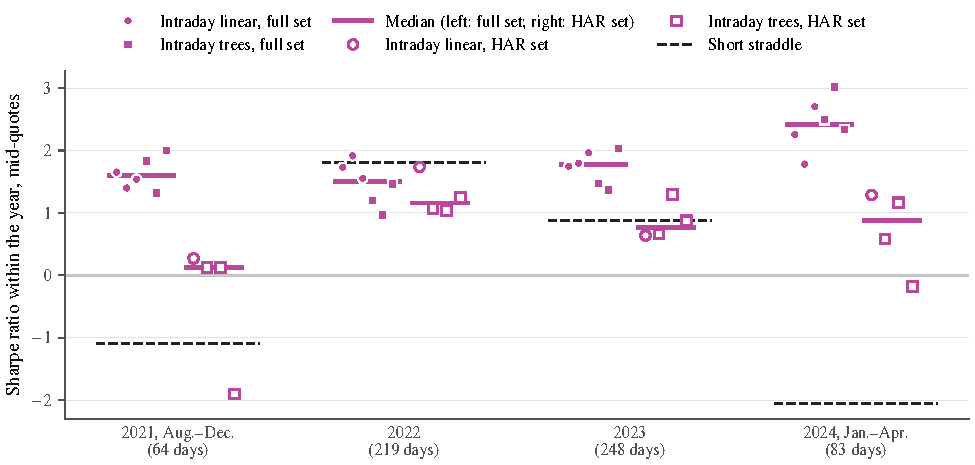
\includegraphics[width=\linewidth]{generated/rehaul_econ_byyear.pdf}
\caption{Sharpe ratio of the sign strategy by calendar year, at mid-quotes, on the \rheSzDays{} post-warmup days of $\mathcal T_{\mathrm{opt}}$. Each point is $\SR_y$, the Sharpe ratio of the year's daily returns annualized by the square root of that year's option days per calendar year (Section~\ref{sec:rh_econ_measures}); the paper's $\SR$ pools the days of all years. Within each year, the left group shows the six intraday forecasts on the full predictor set (filled) and the right group the \rhemHarDistinctWord{} distinct forecasts on the HAR benchmark set (open; the ridge, lasso and elastic net forecasts coincide, Table~\ref{tab:rh_econ_main}); circles are linear models, squares tree ensembles, and the short magenta lines the group medians (full set: \rhemByYearFullMedOne{}, \rhemByYearFullMedTwo{}, \rhemByYearFullMedThree{}, \rhemByYearFullMedFour{}; HAR set: \rhemByYearHarMedOne{}, \rhemByYearHarMedTwo{}, \rhemByYearHarMedThree{}, \rhemByYearHarMedFour{}). The long dashed line marks the short straddle (\rhemByYearShortOne{}, \rhemByYearShortTwo{}, \rhemByYearShortThree{}, \rhemByYearShortFour{}). The years hold \rhemNyOne{}, \rhemNyTwo{}, \rhemNyThree{}, \rhemNyFour{} option days, and the first and last are partial.}
\label{fig:rh_econ_byyear}
\end{figure}

\begin{itemize}
% 2026-10-26 (integration, JFEc): moved here from 07_economics.tex (Performance measures, Annualized Sharpe ratio).
\item \textbf{Annualization.} In the Sharpe ratio $\SR$ of Section~\ref{sec:rh_econ_measures},
  $q = T/\sum_y c_y = \rheAnnDays$, with $\sum_y c_y = \rheAnnYears$ ($c_y = \rheDSixCovOne$, \rheDSixCovTwo,
  \rheDSixCovThree{} and \rheDSixCovFour{} for \rheDSixYearOne{} to \rheDSixYearFour), where $c_y$ runs from the later
  of 1 January and the sample's first day to the earlier of 31 December and its last day. In the ratios $\SR_y$ of
  the single years, $A_y = N_y/c_y$ is \rheDSixAOne, \rheDSixATwo, \rheDSixAThree{} and \rheDSixAFour{}
  ($N_y = \rheDSixNOne$, \rheDSixNTwo, \rheDSixNThree, \rheDSixNFour). The equal-weight mean of the $\SR_y$, an
  alternative in Table~\ref{tab:rh_econ_sharpe_defs}, keeps a year with many option days from dominating the average
  if the strategy's performance changes over the sample.
% 2026-10-28 (D19, standard pooled Sharpe): q of the pooled ratio added; A_y now annualizes the single years only.
% Was: "\item \textbf{Annualization.} In the Sharpe ratio $\SR$ of Section~\ref{sec:rh_econ_measures}, $A_y =
% N_y/c_y$ is \rheDSixAOne, \rheDSixATwo, \rheDSixAThree{} and \rheDSixAFour{} for \rheDSixYearOne{} to
% \rheDSixYearFour{} ($N_y = \rheDSixNOne$, \rheDSixNTwo, \rheDSixNThree, \rheDSixNFour; $c_y = \rheDSixCovOne$,
% \rheDSixCovTwo, \rheDSixCovThree, \rheDSixCovFour), where $c_y$ runs from the later of 1 January and the sample's
% first day to the earlier of 31 December and its last day. Equal weights also keep a year with many option days from
% dominating the average if the strategy's performance changes over the sample."
% 2026-10-26 (integration, JFEc): note D6 resolved (decision of 2026-10-22) and parked; its disclosure is now the item
% below. Was: "\editc{orange}{D6}{Decision (user, 2026-10-22): the Sharpe ratio is the definition above (D6): for each
% calendar year $y$ of the post-warmup sample, $\SR_y = \sqrt{A_y}\,\bar r_y/\mathrm{sd}_y(r)$ with $A_y = N_y/c_y$ the
% year's option days per calendar year, and $\SR$ the equal-weight mean of the $\SR_y$; every statement about a Sharpe
% ratio difference uses the paired block-bootstrap test of Appendix~\ref{sec:rh_methods_tests}, which resamples D6
% itself.\\Disclosure: this definition was adopted after the results under the previous one (the per-year ratio with
% $\sqrt{N_y}$, $N_y$-weighted, of 2026-10-18) had been seen. That ratio (D1) and the ratio of the pooled daily returns
% scaled by $\sqrt{252}$ (D2), with the \citet{LedoitWolf2008} test of the pooled ratios, are reported in
% Table~\ref{tab:rh_econ_sharpe_defs}, together with D6 before and from \rheSplitDate.}"
\item \textbf{When the definition was chosen.} We adopted $\SR$ after the results under two previous definitions had
  been seen: the per-year ratio with $\sqrt{N_y}$ in place of $\sqrt{A_y}$, the years weighted by $N_y$, and then the
  equal-weight mean of the $\SR_y$. Table~\ref{tab:rh_econ_sharpe_defs} therefore repeats the comparison of the full
  predictor set with the HAR benchmark set under both; the paired block-bootstrap test of equal means of the $\SR_y$
  (Appendix~\ref{sec:rh_methods_tests}) rejects at the 5\% level in \rheDefBootSig{} of the \rheDefN{} classes, the
  \citet{LedoitWolf2008} test of equal ratios $\SR$ in \rheDefPoolSig. Under the two alternatives the short
  straddle's mid-quote ratio is \rhemShDSixShort{} and \rhemShDOneShort{} rather than \rheShortSh.
% 2026-10-28 (D19, standard pooled Sharpe): the pooled ratio is now SR itself; D6 (the equal-year mean) joins D1 as an
% alternative. Was: "We adopted $\SR$ after the results under a previous definition had been seen: the per-year ratio
% with $\sqrt{N_y}$ in place of $\sqrt{A_y}$, the years weighted by $N_y$. Table~\ref{tab:rh_econ_sharpe_defs}
% therefore repeats the comparison of the full predictor set with the HAR benchmark set under that ratio and under the
% ratio of the mean to the standard deviation of all \rheSzDays{} daily returns, scaled by $\sqrt{252}$, with the
% \citet{LedoitWolf2008} test of equal pooled ratios; the latter rejects at the 5\% level in \rheDefLWSig{} of the
% \rheDefN{} classes. Under the two alternatives the short straddle's mid-quote ratio is \rhemShDOneShort{} and
% \rhemShDTwoShort{} rather than \rheShortSh."
% 2026-10-26 (integration, JFEc): moved here from 07_economics.tex (Robustness checks, Subsample stability).
\item \textbf{Subsamples.} Table~\ref{tab:rh_econ_sharpe_defs} also computes $\SR$ separately on the post-warmup
  days before and from \rheSplitDate, when CBOE expanded SPXW expirations to all five weekdays, each subsample with
  its own $q$ (\rheAnnDaysPre{} and \rheAnnDaysPost).
% 2026-10-28 (D19, standard pooled Sharpe): ", each subsample with its own $q$ (...)" added.
\end{itemize}

% 2026-10-26 (integration, JFEc): moved here from 07_economics.tex (Trading strategies: the robust clip and the
% percentile rank; Sizing sample; Results: Position sizing). Code: the rank uses <= (rows.py:1044); rules at
% rows.py:88-134, 1028-1062. The full long, scaled short rule stays parked (2026-10-18, N11; \rheSzLfssMed unused).
\subsection{Position sizing}
\label{app:rh_econ_sizing}
% 2026-10-26 (integration, coordinator: bullet structure): the lead sentence and the two rules recast as one
% bold-lead item with sub-items, content kept.
\begin{itemize}
\item \textbf{Sized rules.} Besides the sign strategy of Section~\ref{sec:rh_econ_strategy}, two rules scale the
  position by the size of the variance gap.
  \begin{itemize}
  \item \emph{Robust clip:} $q_t = \clip\bigl((\hat\sigma^2_t - \mathrm{IV}_t^2)/\mathrm{MAD}_t, -1, 1\bigr)$, where
    $\mathrm{MAD}_t = \operatorname{median}_{t'<t}\bigl|\hat\sigma^2_{t'} - \mathrm{IV}_{t'}^2\bigr|$ is the expanding
    median absolute variance gap over earlier days $t' < t$ in $\mathcal T_{\mathrm{opt}}$.
  \item \emph{Percentile rank:} the sign of the gap scaled by the empirical percentile rank of its magnitude across
    the $t - 1$ preceding days $t' < t$ in $\mathcal T_{\mathrm{opt}}$:
    \[
      q_t = \sign\bigl(\hat\sigma^2_t - \mathrm{IV}_t^2\bigr)\cdot\frac{1}{t-1}\sum_{t'<t}
        \mathbf{1}\bigl\{|\hat\sigma^2_{t'} - \mathrm{IV}_{t'}^2| \le |\hat\sigma^2_t - \mathrm{IV}_t^2|\bigr\}.
    \]
  \end{itemize}
\item \textbf{Sizing sample.} Every position $q_t$ uses days $t' < t$ only. The first \rheSzWarmup{} days of
  $\mathcal T_{\mathrm{opt}}$ initialize $\mathrm{MAD}_t$, and every rule, the sign strategy included, is evaluated
  on the remaining \rheSzDays{} post-warmup days.
% 2026-10-26 (integration, JFEc; audit results-12): the twelve forecasts count the identical HAR-set linear forecast
% three times; flagged in the text. The medians and counts over the distinct forecasts need new macros (NUMBERS).
\item \textbf{Results.} Across the \rhrPoolN{} pooled forecasts, in which the identical HAR-set ridge, lasso and
  elastic-net forecast is counted three times (Table~\ref{tab:rh_econ_main}, note b), the median mid-quote Sharpe
  ratio is \rhrPoolSzSignMed{} under the sign strategy, \rhrPoolSzClipMed{} under the robust clip and
  \rhrPoolSzRankMed{} under the percentile rank. In point estimates the robust clip beats the sign strategy
  ($\SR^{\mathrm{clip}} > \SR^{\mathrm{sign}}$) for \rhrPoolSzClipBeats{} of the \rhrPoolN{} forecasts.
\end{itemize}

% 2026-10-26 (integration, JFEc): moved here from 07_economics.tex (Performance measures: Compounding and the drawdown
% item; Robustness checks: Compounded wealth). Code: experiments/close_compounding_headline.py:140-153 (wealth_stats);
% the pooled values from writeup/make_rehaul_pooled_extras.py (\rhpc...). Ruin bound f < 1/|min_t r_t|.
\subsection{Compounded wealth}
\label{app:rh_econ_compounding}
\begin{itemize}
\item \textbf{Definition.} From initial capital $V_0 = 1$, a fixed fraction $f = \rhappCompF\%$ of current wealth
  is allocated to the straddle premium each day, which gives the terminal portfolio value and the annualized log
  growth rate
  \[
  V = \prod_{t \in \mathcal T_{\mathrm{opt}}^{+}}\bigl(1 + f\,r_t\bigr),
  \qquad
  G = \frac{252}{\rheSzDays}\sum_{t \in \mathcal T_{\mathrm{opt}}^{+}}\log\bigl(1 + f\,r_t\bigr).
  \]
  At quoted bid/ask prices $r^{\mathrm{ba}}_t$ replaces $r_t$. The maximum drawdown is
  $\max_t\bigl(1 - V_t/\max_{t'\le t}V_{t'}\bigr)$, with $V_t$ the portfolio value at the end of day $t$.
% 2026-10-26 (integration, JFEc; audit results-16): the short straddle's values are not in
% Table tab:rh_pooled_shift_compounding, so the citation now covers the pooled forecasts only (a short-straddle row
% is requested from NUMBERS). Was: "... against \rhpcAW{} and \rhpcAWX{} for the unconditional short straddle, with
% maximum drawdowns reaching up to \rhpcDDMaxMid\% and \rhpcDDMaxX\%, respectively (\rhpcADDMid\% and \rhpcADDX\% for
% the unconditional short straddle; Table~\ref{tab:rh_pooled_shift_compounding});"
\item \textbf{Results.} Across the \rhpsNfc{} pooled forecasts (the HAR-set linear forecast counted three times),
  compounding at $f = \rhappCompF\%$ over the \rhpcNdays{} post-warmup days yields a median terminal value $V$ of
  \rhpcWMedMid{} at mid-quotes (\rhpcWLoMid{} to \rhpcWHiMid) and \rhpcWMedX{} at quoted bid/ask prices (\rhpcWLoX{}
  to \rhpcWHiX), with maximum drawdowns of up to \rhpcDDMaxMid\% and \rhpcDDMaxX\%
  (Table~\ref{tab:rh_pooled_shift_compounding}). The unconditional short straddle ends at $V = \rhpcAW$ and
  \rhpcAWX, with maximum drawdowns of \rhpcADDMid\% and \rhpcADDX\%.
\end{itemize}

% 2026-10-26 (integration, JFEc): moved here from 07_economics.tex (Robustness checks, Interval-shift test). Code:
% writeup/make_rehaul_pooled_extras.py (\rhps...); the shifted row is placed as yhat_{c+j}^2 s^2_c.
\subsection{Interval-shift test}
\label{app:rh_econ_shift}
% 2026-10-26 (integration, coordinator: bullet structure): the subsection's prose recast as bold-lead items, content
% kept.
\begin{itemize}
\item \textbf{The shifted sign rule.} We replace $\hat y_{t,c}$ in the sign rule by the forecast $\hat y_{t,c+j}$ from
  $j$ half-hour bars away,
  \[
    q_t = \sign\bigl(\hat y_{t,c+j}^{\,2}\, s^2_{t,c} - \mathrm{IV}_t^2\bigr), \qquad j = \rhpsJMin, \dots, \rhpsJMax,
  \]
  ($j < 0$ earlier on day $t$; $j > 0$ on day $t+1$, not known at the 15:30 origin, a placebo).
\item \textbf{Across offsets.} The median Sharpe ratio across the \rhpsNfc{} pooled forecasts (\rhpsNdays{}
  post-warmup days on which every shifted forecast exists; \rhpsZeroMed{} at $j = 0$) ranges from \rhpsMedLo{} to
  \rhpsMedHi{} across $j$ (a half-range of $\pm\rhpsHalf$), against the $\pm\rhpsNoiseBand$ 95\% sampling band of the
  Sharpe ratio under i.i.d.\ returns (Table~\ref{tab:rh_pooled_shift_compounding}).
% 2026-10-26 (integration, JFEc; audit results-15): parked -- "lowers the median, by" described the median of the
% per-forecast changes as the change of the median. Was: "Every earlier bar ($j < 0$) lowers the median, by
% \rhpsSameDeltaLo{} to \rhpsSameDeltaHi{} against $j = 0$, and at each earlier bar between \rhpsStaleNBelowMin{} and
% \rhpsStaleNBelowMax{} of the \rhpsNfc{} forecasts have a lower Sharpe ratio than at $j = 0$;"
\item \textbf{Earlier bars.} At the earlier bars ($j < 0$) the median across forecasts of the change in each
  forecast's Sharpe ratio against $j = 0$ runs from \rhpsSameDeltaLo{} to \rhpsSameDeltaHi, and at each earlier bar
  between \rhpsStaleNBelowMin{} and \rhpsStaleNBelowMax{} of the \rhpsNfc{} forecasts have a lower Sharpe ratio than
  at $j = 0$.
\end{itemize}
% 2026-10-26 (integration, JFEc): note E26b parked here as an open decision (James); it is already listed in
% rehaul/99_author_notes.tex ("Open decisions for James": the pooled interval-shift test), whose reference should now
% point to app:rh_econ_shift (FRONT). Was: "\editc{orange}{E26b}{Decision: to decide (James).\\Open choices for the
% interval-shift test: (i) the days: every $j$ on the \rhpsNdays{} days on which every shifted forecast exists (above;
% the original test's rule, which drops the last option day, \rhoosSpanEnd, as it has no next session; median Sharpe
% ratio at $j = 0$: \rhpsZeroMed), or only $j \le 0$ on all \rhpsPwNdays{} post-warmup days of the printed Sharpe
% ratios (median at $j = 0$: \rhpsPwZeroMed, range \rhpsPwMedLo{} to \rhpsPwMedHi, half-range $\pm\rhpsPwHalf$); (ii)
% the sampling band: $1.96\sqrt{\sum_y A_y/N_y}/K$ over the $K$ calendar years, the i.i.d.\ band of the Sharpe ratio
% of note D6 at $\SR = 0$, in place of the original $1.96\sqrt{252/n}$ (writeup/make\_rehaul\_pooled\_extras.py);
% (iii) how to read the pattern for $j < 0$. The earlier reading (``well within'' the band, ``consistent with
% sampling variation'') is parked.}"

% 2026-10-26 (integration, JFEc): added from drafts/2026-10-25_econ_main.tex (Execution costs and break-even spreads);
% the closing-interval HAR item is parked (plan D2). Was (its second sub-item): "For the closing-interval HAR forecast
% the two factors are \rhemBeMeanCiHar{} and \rhemBeShCiHar{} (\rhemBeMeanPctCiHar\% and \rhemBeShPctCiHar\% of the
% premium); for the \rhemHarDistinctWord{} distinct HAR-set forecasts the Sharpe-ratio factor runs from
% \rhemBeShHarMin{} to \rhemBeShHarMax." "Trading at quoted bid/ask prices lowers every strategy's Sharpe ratio" is
% asserted in make_rehaul_econ_main.py (DRAFT CLAIMS).
\subsection{Execution costs and break-even spreads}
\label{app:rh_econ_breakeven}
% 2026-10-26 (integration, coordinator: bullet structure): the lead prose recast as two bold-lead items, the three
% results as sub-items of the second; content kept.
\begin{itemize}
\item \textbf{Quoted spreads.} Trading at quoted bid/ask prices rather than mid-quotes lowers every strategy's Sharpe
  ratio (Table~\ref{tab:rh_econ_main}). The median quoted half-spread of the straddle is \rhemHalfSpreadMed\% of the
  premium on the \rheSzDays{} post-warmup days (\rhemHalfSpreadMedAll\% on all \cmNdays{} days of
  $\mathcal T_{\mathrm{opt}}$).
\item \textbf{Break-even spreads.} We scale every day's quoted half-spread $h_t = (P^{a}_t - P^{b}_t)/2$ by a common
  factor $k$, so that a purchase pays $P_t + k h_t$ and a sale receives $P_t - k h_t$ ($k = 0$: mid-quotes; $k = 1$:
  quoted bid/ask prices), and find the factor at which the mean daily return, and with it the Sharpe ratio, reaches
  zero; in percent of the premium, the break-even half-spread is $k$ times the median quoted half-spread.
  \begin{itemize}
  \item For the six full-set forecasts the mean daily return, and with it the Sharpe ratio, stays positive up to
    $k = \rhemBeMeanFullMin$ to $\rhemBeMeanFullMax$ (\rhemBeMeanFullMinPct\% to \rhemBeMeanFullMaxPct\% of the
    premium).
  \item For the benchmark forecast the factor is \rhemBeMeanRidgeHar{} (\rhemBeMeanPctRidgeHar\% of the premium); for
    the \rhemHarDistinctWord{} distinct HAR-set forecasts it runs from \rhemBeMeanHarMin{} to \rhemBeMeanHarMax.
  \item The mean daily return of the short straddle, and with it its Sharpe ratio, reaches zero at
    $k = \rhemBeMeanShort$, inside the quoted spread.
  \end{itemize}
% 2026-10-28 (D19, standard pooled Sharpe): the pooled ratio has the sign of the mean, so the two break-even factors
% coincide (\rhemBeSh... = \rhemBeMean...), and the short straddle's ratio is positive at mid-quotes (\rheShortSh).
% Was: "find the factor at which the mean daily return or the Sharpe ratio reaches zero"; "For the six full-set
% forecasts the mean daily return stays positive up to $k = \rhemBeMeanFullMin$ to $\rhemBeMeanFullMax$
% (\rhemBeMeanFullMinPct\% to \rhemBeMeanFullMaxPct\% of the premium) and the Sharpe ratio up to $k = \rhemBeShFullMin$
% to $\rhemBeShFullMax$ (\rhemBeShFullMinPct\% to \rhemBeShFullMaxPct\%)."; "For the benchmark forecast the two factors
% are \rhemBeMeanRidgeHar{} and \rhemBeShRidgeHar{} (\rhemBeMeanPctRidgeHar\% and \rhemBeShPctRidgeHar\% of the
% premium); for the \rhemHarDistinctWord{} distinct HAR-set forecasts the Sharpe-ratio factor runs from
% \rhemBeShHarMin{} to \rhemBeShHarMax."; "The mean daily return of the short straddle reaches zero at
% $k = \rhemBeMeanShort$, inside the quoted spread, and its Sharpe ratio is negative at mid-quotes already."
\end{itemize}

% 2026-10-26 (integration, JFEc): moved here from 07_economics.tex (Performance measures: Elementary score and
% Decision-threshold property; Results: Statistical accuracy versus economic value). Code:
% experiments/close_murphy_splits_headline.py:227-230, called as elementary(plain / iv_var, target / iv_var, 1.0);
% the pooled correlations from make_rehaul_economics.py (pooled_rank_series, \rheRankCorr...Pool).
\subsection{Forecast loss and economic value}
\label{app:rh_econ_rankcorr}
\begin{itemize}
\item \textbf{Elementary score.} To measure forecast accuracy at the decision threshold $\mathrm{IV}_t^2$, we
  evaluate the elementary score of \citet{Ehm2016} normalized by implied variance,
  \[
  \mathrm{ES}_{1,t} = \Bigl|\frac{\RV_t}{\mathrm{IV}_t^2} - 1\Bigr|\;
    \mathbf{1}\bigl\{\min(\hat\sigma^2_t, \RV_t) \le \mathrm{IV}_t^2 < \max(\hat\sigma^2_t, \RV_t)\bigr\},
  \]
  and denote its mean over the post-warmup days $\mathcal T_{\mathrm{opt}}^{+}$ by $\overline{\mathrm{ES}}_1$.
  $\mathrm{ES}_{1,t}$ is positive if and only if the forecast $\hat\sigma^2_t$ and the realization $\RV_t$ fall on
  opposite sides of the implied variance, that is, precisely when the sign strategy takes the wrong side.
% 2026-10-26 (integration, JFEc; audit results-12, results-13): the two caveats added -- the mean QLIKE covers all
% T_opt days incl. the warm-up (make_rehaul_economics.py ~3046-3049: ql_p over N_OPT, es_p over iloc[WARMUP:]), and
% the twelve points hold a three-way tie. Regenerating \rheRankCorrQPool* on the post-warmup days and over the
% distinct forecasts is requested from NUMBERS.
\item \textbf{Rank correlations.} Across the \rhrPoolN{} pooled forecasts, the rank correlation of the Sharpe ratio is
  positive with average QLIKE loss, \rheRankCorrQPool, and negative with $\overline{\mathrm{ES}}_1$, the loss at the
  implied-variance threshold, \rheRankCorrESPool. With the per-year ratio scaled by $\sqrt{N_y}$ and weighted by
  $N_y$ in place of $\SR$, the two correlations are \rheRankCorrQPoolDOne{} and \rheRankCorrESPoolDOne; with the
  equal-weight mean of the $\SR_y$, they are \rheRankCorrQPoolDSix{} and \rheRankCorrESPoolDSix.
  Their signs are the same under all three definitions.
% 2026-10-28 (D19, standard pooled Sharpe): the pooled ratio scaled by sqrt(252) ranks as SR does; the third definition
% is now D6. Was: "with the ratio of the pooled daily returns scaled by $\sqrt{252}$, they are \rheRankCorrQPoolDTwo{}
% and \rheRankCorrESPoolDTwo." Two caveats: the mean QLIKE loss is taken over all \cmNdays{}
  days of $\mathcal T_{\mathrm{opt}}$, the \rheSzWarmup{} warm-up days included, while $\overline{\mathrm{ES}}_1$ and
  the Sharpe ratio are on the \rheSzDays{} post-warmup days; and the \rhrPoolN{} forecasts count the identical
  HAR-set ridge, lasso and elastic-net forecast three times, a three-way tie in both rankings.
\end{itemize}

% 2026-10-26 (integration, JFEc): moved here from 07_economics.tex (Robustness checks, Window length). Macros
% \rhrb... from writeup/make_rehaul_robust_window.py (\rhrbMaxAbsDSRMid = \rhrbDSRRfHarMid: the forest on the HAR
% benchmark moves most).
\subsection{A longer estimation window}
\label{app:rh_econ_robust}
% 2026-10-26 (integration, coordinator: bullet structure): the prose recast as a bold-lead item with sub-items.
\begin{itemize}
\item \textbf{Window of \rhrbWinLong{} trading days.} With a rolling window of \rhrbWinLong{} trading days in place of
  \rhrbWinMain{} (Table~\ref{tab:rh_robust_w3500}):
  \begin{itemize}
  \item the full predictor set raises the mid-quote Sharpe ratio in \rhrbNDSRFPosMidLong{} of the
    \rhrbNModelsLong{} model classes, \rhrbNDSRFSigMidLong{} of them significantly at the 5\% level;
  \item no pooled forecast's Sharpe ratio differs significantly between the two windows (\rhrbNSRSigMid{} of
    \rhrbNArms), and the random forest on the HAR benchmark set moves most, from \rhrbSRRfHarMidMain{} to
    \rhrbSRRfHarMidLong{} (\rhrbPSRRfHarMid).
  \end{itemize}
\end{itemize}

% 2026-10-26 (integration, JFEc): added from drafts/2026-10-25_econ_decomp.tex (generator
% writeup/make_rehaul_econ_decomp.py, \rhed... macros), lightly edited: "HAR twin" -> the HAR-set forecast of the same
% class; the worthless-expiry item now carries the share that the parked "Concentration of economic gains" item of
% 07_economics.tex printed (without its "settlement pinning" gloss: audit numbers-1, results-6, correctness-8).
% 2026-10-28 (author: conventional titles). Was: \subsection{Where the profits come from}
\subsection{Profit decomposition}
\label{app:rh_econ_decomp}
\begin{itemize}
\item \textbf{A short straddle that turns long on a fifth of the days.} The sign strategies of the six pooled
  forecasts on the full predictor set hold a long straddle on \rhedLongNMin{} to \rhedLongNMax{} of the \rheSzDays{}
  post-warmup days (\rhedLongPctMin--\rhedLongPctMax\%; Table~\ref{tab:rh_econ_longshort}). Because
  \[
    r_t = q_t R_t = -R_t + 2R_t\,\mathbf{1}\{q_t = +1\},
  \]
  each strategy's return is that of the unconditional short straddle plus a gain $\Delta_t = 2R_t\mathbf{1}\{q_t = +1\}$
  over it, and that gain is earned on the long days only.
  \begin{itemize}
  \item The unconditional short straddle earns \rhedUncShortMean\% of the premium a day at mid-quotes; the gain on the
    long days adds \rhedGainMin--\rhedGainMax\%, which is \rhedGainShareMin--\rhedGainShareMax\% of the strategies'
    mean daily return of \rhedMeanMin--\rhedMeanMax\%.
  \item On its long days the straddle returns \rhedLongMidMin--\rhedLongMidMax\% of the premium on average at
    mid-quotes and \rhedLongBaMin--\rhedLongBaMax\% bought at the ask. On the remaining days the short straddle earns
    \rhedShortMidMin--\rhedShortMidMax\% at mid-quotes, against \rhedUncShortMean\% on all days: the long days are the
    days on which the short straddle loses.
  \item The long days account for \rhedLongShareMin--\rhedLongShareMax\% of the summed mid-quote return
    (\rhedLongShareXMin--\rhedLongShareXMax\% at quoted bid/ask prices). On the HAR benchmark set the same model
    classes go long on \rhedHarLongNMin{} to \rhedHarLongNMax{} days, on which the straddle returns only
    \rhedHarLongMidMin--\rhedHarLongMidMax\% (gain over the short straddle \rhedHarGainMin--\rhedHarGainMax\% a day).
  \end{itemize}
\item \textbf{No better call of the premium's sign, but the large moves.} The position has the sign of
  $\RV_t - \mathrm{IV}_t^2$ on \rhedHitMin--\rhedHitMax\% of the days, against \rhedUncShortHit\% for the
  unconditional short straddle, so the forecasts are no better than always selling at calling the sign of the
  realized premium. What they add is in the long days: realized variance exceeds implied variance on
  \rhedLongHitMin--\rhedLongHitMax\% of them, against \rhedUncRVAboveIV\% of all days, yet the long straddle has a
  positive return on only \rhedLongPosMin--\rhedLongPosMax\% of its long days, so its mean return on those days comes
  from a few large moves.
\item \textbf{Forecast quintiles} (Table~\ref{tab:rh_econ_quintiles}). Sorted by the forecast variance gap
  $\log(\hat\sigma^2_t/\mathrm{IV}_t^2)$, the mean ratio of realized to implied variance rises from quintile to
  quintile for \rhedQMonoN{} of the \rhedNFull{} full-set forecasts, from \rhedQOneRVIV{} in the lowest to \rhedQFiveRVIV{} in the
  highest (mean of the six), and for \rhedHarQMonoN{} of the six HAR-set forecasts (\rhedHarQOneRVIV{} to
  \rhedHarQFiveRVIV): the forecasts rank the closing half hours by their realized variance relative to the implied.
  \begin{itemize}
  \item The return of a long straddle is negative in each of the four lower quintiles (\rhedQLowRMin{} to
    \rhedQLowRMax\% on average) and \rhedQFiveR\% in the highest, where \rhedQFiveLong\% of the days are long days;
    for the HAR-set forecasts it is \rhedHarQFiveR\%. The sign rule's threshold, $\hat\sigma^2_t =
    \mathrm{IV}_t^2$, falls between the fourth quintile (forecast ratio \rhedQFourFc) and the fifth
    (\rhedQFiveFc).
  \item The highest quintile earns \rhedQFiveShare\% of the summed mid-quote return of the six full-set strategies
    (\rhedQFiveShareRngMin--\rhedQFiveShareRngMax\% across them), against \rhedHarQFiveShare\% for the HAR benchmark
    set. Across the four lower quintiles, where the strategies are short, the return is not monotone in the forecast.
  \end{itemize}
\item \textbf{About ten days carry the gain over the short straddle} (Table~\ref{tab:rh_econ_bestdays}). The six
  full-set forecasts share \rhedBestAllSix{} of their ten best days and \rhedWorstAllSix{} of their ten worst; the
  best days are long straddles on large closing moves, the worst are short straddles on large closing moves.
  \begin{itemize}
  \item Without each forecast's ten best days, the Sharpe ratio gain over the unconditional short straddle falls from
    \rhedDShortAllMin--\rhedDShortAllMax{} to \rhedDShortExBestMin{} to \rhedDShortExBestMax{} (negative for
    \rhedDShortExBestNeg{} of the \rhedNFull); the ten days earn \rhedBestShareMin--\rhedBestShareMax\% of the summed return
    gain over the short straddle, so the other long days lose on balance.
  \item The largest, \rhedTopDate, returned \rhedTopR\% of the premium on a closing-half-hour move of
    \rhedTopMove\% (realized variance \rhedTopRVIV{} times the implied), \rhedTopShareMin--\rhedTopShareMax\% of each
    full-set strategy's summed return.
  \item Against the HAR-set forecast of the same class the gain is less concentrated: without the forecast's ten best
    days the Sharpe ratio gain falls from \rhedDHarAllMin--\rhedDHarAllMax{} to \rhedDHarExBestMin--\rhedDHarExBestMax,
    and those days carry \rhedHarBestShareMin--\rhedHarBestShareMax\% of the summed return gain over it.
  \end{itemize}
\item \textbf{The days are not scheduled announcements.} Of the \rhedBestUnion{} days in the union of the six
  forecasts' best days, \rhedBestFomcN{} is an FOMC statement day and \rhedBestNoTagN{} carry no tag in our event
  calendar, \rhedBestAfterRelN{} of them after \rhedRelEndText, when its macro-release dates end (its FOMC dates are
  complete).
  \begin{itemize}
  \item On the \rhedFomcN{} FOMC statement days the closing straddle returns \rhedFomcR\% on average
    ($t = \rhedFomcRT$, the days treated as independent); the full-set forecasts are long on \rhedFomcLong\% of them
    and earn \rhedFomcStrat\% a day, against \rhedFomcOtherStrat\% on the other days.
  \item On the \rhedMeN{} month ends the straddle returns \rhedMeR\% ($t = \rhedMeRT$) and the squared closing move
    averages \rhedMeMoveSqIV{} times the implied variance; the forecasts are long on \rhedMeLong\% of them, earn
    \rhedMeStrat\% a day, and \rhedMeShare\% of their summed return comes from these days (\rhedWorstMeN{} of the
    worst days are month ends).
  \item On the \rhedOpexN{} monthly SPX expirations the straddle returns \rhedOpexR\% ($t = \rhedOpexRT$); the
    forecasts are long on \rhedOpexLong\% of them and earn \rhedOpexShare\% of their summed return there, a gain the
    unconditional short straddle shares.
  \end{itemize}
\item \textbf{Calibration and the short tilt} (Table~\ref{tab:rh_econ_longshort}, Panel D). In levels the full-set
  forecasts are close to unbiased on the option days (mean forecast over mean realized variance
  \rhedCalLevelMin--\rhedCalLevelMax), but in ratios they are low: the mean of $\RV_t/\hat\sigma^2_t$, the scale that
  minimizes mean QLIKE, is \rhedCalScaleMin--\rhedCalScaleMax, the downward bias of squaring a level forecast
  (Section~\ref{sec:rh_methods_setup}).
  \begin{itemize}
  \item Multiplying each forecast by a causal estimate of that scale, the mean of $\RV_{t'}/\hat\sigma^2_{t'}$ over the
    earlier option days $t' < t$, changes \rhedBcFlipMin{} to \rhedBcFlipMax{} positions, all from short to long.
    The straddle's mean return on the changed days is \rhedBcFlipRMin{} to \rhedBcFlipRMax\%, and the Sharpe ratio
    falls to \rhedBcShMin--\rhedBcShMax{} at mid-quotes and \rhedBcShXMin--\rhedBcShXMax{} at quoted bid/ask prices
    (below the uncorrected ratio for \rhedBcShDownN{} of the six; the correction raises it for \rhedHarBcShUpN{} of
    the six HAR-set forecasts). This is a diagnostic, not a strategy of the paper.
  \item A reading consistent with this: a straddle pays the absolute move of the index, so a long position is
    profitable when the expected realized volatility, not variance, exceeds the implied volatility. The sign rule
    $\hat\sigma^2_t > \mathrm{IV}_t^2$ is the same as $\hat y_t\, s_{t,c} > \mathrm{IV}_t$, a comparison of the level
    forecast with the implied volatility, which the uncorrected forecast makes.
  \item The forecast target and the straddle's settlement differ: $\RV_t$, the realized variance of the futures from
    one-minute returns, averages \rhedUncRVIVMean{} of the implied variance (median \rhedUncRVIVMed), while the squared
    log move of the cash index from $S_t$ to $S^{\mathrm{close}}_t$ averages \rhedMoveSqIV{} of it, and
    \rhedMoveSqRV{} times the mean of $\RV_t$. Measured on the move that settles the straddle, the implied variance
    carries no premium on average in our sample, which agrees with the short straddle's Sharpe ratio of
    \rheShortSh, whose mean daily return is not significantly different from zero ($t = \rheShortT$).
% 2026-10-28 (D19, standard pooled Sharpe): the short straddle's ratio is now positive; its insignificance added.
% Was: "which agrees with the short straddle's Sharpe ratio of \rheShortSh."
  \end{itemize}
% 2026-10-26 (integration, JFEc; audit numbers-1, results-6, correctness-8): the worthless-expiry share of the parked
% "Concentration of economic gains" item (07_economics.tex) placed here, its "settlement pinning" gloss dropped; the
% share is over the \rhrPoolN{} pooled forecasts (the HAR-set linear forecast counted three times).
\item \textbf{Worthless expiries are not pinning.} $R_t = -1$ exactly when the close settles between the two strikes,
  $K_P \le S^{\mathrm{close}}_t \le K_C$; on \rhedGapFiveN{} of the \rheSzDays{} days the two strikes are 5 index
  points apart, against a median one-standard-deviation implied move over the half hour of \rhedMoveSdPts{} points.
  \begin{itemize}
  \item The straddle expires worthless on \rhedWorthN{} days (\rhedWorthPct\%). A normal half-hour log move with the
    implied volatility $\mathrm{IV}_t$ predicts \rhedWorthExpIV{} such days (\rhedWorthExpIVPct\%; the difference is
    \rhedWorthZ{} standard deviations), the empirical distribution of the earlier days' moves scaled by
    $\mathrm{IV}_t$ predicts \rhedWorthExpEmp, and the close is uniformly placed between adjacent strikes (mean
    distance to the nearest strike \rhedStrikeDist{} points, \rhedStrikeDistUnif{} under a uniform;
    Kolmogorov--Smirnov $D = \rhedKsD$, 5\% critical value \rhedKsCV).
  \item The full-set forecasts are short on \rhedWorthShortMin--\rhedWorthShortMax{} of these days, on which the short
    straddle keeps its whole premium; these days supply \rhePoolWorthlessShareMed\% of the positive returns of the
    median pooled forecast (\rhePoolWorthlessShareMin--\rhePoolWorthlessShareMax\% across the \rhrPoolN{} pooled
    forecasts).
  \item Monthly SPX expirations are the exception: \rhedWorthOpexN{} of the \rhedOpexN{} expire worthless against
    \rhedWorthOpexExp{} expected ($\rhedWorthOpexZ$ standard deviations), and the squared closing move averages
    \rhedOpexMoveSqIV{} of the implied variance. Outside them the share is \rhedWorthOtherPct\% against
    \rhedWorthOtherExpPct\% expected.
  \end{itemize}
\item \textbf{Risk exposures} (Table~\ref{tab:rh_econ_riskreg}; $t$-statistics with Newey--West standard errors at
  bandwidth $S = \rheHACS$ and fixed-$b$ critical values, Appendix~\ref{sec:rh_methods_tests}).
  \begin{itemize}
  \item On the short-straddle return the full-set strategies load \rhedRegBetaShortMin--\rhedRegBetaShortMax{}
    ($t$ from \rhedRegBetaShortTMin{} to \rhedRegBetaShortTMax; $R^2$ \rhedRegRsqAMin--\rhedRegRsqAMax), with
    $\alpha = \rhedRegAlphaAMin$--\rhedRegAlphaAMax\% of the premium a day at mid-quotes (fixed-$b$ $p$ from
    \rhedRegAlphaAPMin{} to \rhedRegAlphaAPMax) and \rhedRegAlphaAXMin--\rhedRegAlphaAXMax\% at quoted bid/ask prices
    ($p$ from \rhedRegAlphaAXPMin{} to \rhedRegAlphaAXPMax). The equal-weight mean of the six returns has
    $\alpha = \rhedRegAvgAlphaA\%$ ($p = \rhedRegAvgAlphaAP$) at mid-quotes and $\rhedRegAvgAlphaAX\%$
    ($p = \rhedRegAvgAlphaAXP$) at quoted bid/ask prices.
  \item They are short volatility, less so than the short straddle: a basis point of absolute S\&P~500 move over the
    closing half hour changes their return by \rhedRegBetaAbsMin{} to \rhedRegBetaAbsMax\% of the premium ($t$ from
    \rhedRegBetaAbsTMin{} to \rhedRegBetaAbsTMax); for their mean return the coefficient, \rhedRegAvgBetaAbs\%, is
    \rhedRegAbsRatio\% of the short straddle's \rhedRegShortBetaAbs\%. The sign of the move does not matter
    (coefficients \rhedRegBetaMoveMin{} to \rhedRegBetaMoveMax).
  \item The S\&P~500 daily return and the change in the VIX explain none of their return ($R^2$
    \rhedRegRsqCMax), and with all regressors $\alpha$ is \rhedRegAlphaDMin--\rhedRegAlphaDMax\% at mid-quotes and
    \rhedRegAlphaDXMin--\rhedRegAlphaDXMax\% at quoted bid/ask prices.
  \item Without each forecast's ten best days, $\alpha$ on the short straddle is \rhedRegAlphaAExBestMin{} to
    \rhedRegAlphaAExBestMax\% ($p \ge \rhedRegAlphaAExBestPMin$). The standard errors allow for serial correlation,
    not for a return distribution whose mean rests on ten days. The HAR-set strategies have
    $\alpha = \rhedHarRegAlphaAMin$--\rhedHarRegAlphaAMax\% ($p \ge \rhedHarRegAlphaAPMin$).
  \end{itemize}
% 2026-10-26 (integration, coordinator: bullet structure): the closing paragraph of the draft recast as a bold-lead
% item with sub-items, content kept.
\item \textbf{Summary: where the profits come from.} The strategy is a short straddle on most days, and the short
  straddle by itself earns nothing detectable in our sample (\rheShortSh{} at mid-quotes, \rheShortShX{} at quoted
  bid/ask prices).
  \begin{itemize}
  \item The profit comes from the days on which the full-set forecasts switch to a long straddle: these are the
    closing half hours that the forecasts rank highest in realized relative to implied variance, the ranking is
    monotone across the forecast quintiles, and on these days the straddle earns \rhedLongMidMin--\rhedLongMidMax\%
    of its premium on average (\rhedQFiveR\% in the top forecast quintile, against \rhedHarQFiveR\% on the HAR
    benchmark set).
  \item The strategy is not a disguised short-volatility position: it has less than half of the short straddle's
    exposure to the size of the closing move, almost none to its return, and none to the market or the VIX.
  \item But the payoff of the ranking is concentrated in about ten days with closing moves several times the
    implied, the same days for all six forecasts, and only \rhedBestFomcN{} of the \rhedBestUnion{} an FOMC statement
    day; without them the gain over the short straddle and the regression $\alpha$ disappear.
  \item The forecasts thus time the sign of the closing-half-hour variance premium in a narrow sense, by stepping out
    of the short straddle on a minority of days, and in this sample of \rheSzDays{} days that timing paid through a
    handful of large closing moves that they anticipated, not through a steady premium.
  \end{itemize}
\end{itemize}

% AUTO-GENERATED by writeup/make_rehaul_econ_decomp.py -- do not edit; re-run the script.
% Table tab:rh_econ_longshort: long and short days of the sign strategy, the gain over the short straddle, and
% the calibration of the forecasts (writeup/make_rehaul_econ_decomp.py, statistics 1 and 3).
\ifdefined\rhedNDays\else% AUTO-GENERATED by writeup/make_rehaul_econ_decomp.py -- do not edit; re-run the script.
% \rhed... macros: where the straddle strategy's profits come from (Section 7 decomposition).
\providecommand{\rhedNDays}{}\renewcommand{\rhedNDays}{614}  % post-warmup option days (= rheSzDays)
\providecommand{\rhedNFull}{}\renewcommand{\rhedNFull}{6}  % pooled intraday forecasts on the full predictor set
\providecommand{\rhedNTop}{}\renewcommand{\rhedNTop}{10}  % best / worst days per forecast
\providecommand{\rhedUncRVAboveIV}{}\renewcommand{\rhedUncRVAboveIV}{28.2}  % % of the 614 days with RV_t > IV_t^2
\providecommand{\rhedUncRVIVMean}{}\renewcommand{\rhedUncRVIVMean}{0.87}  % mean RV_t / IV_t^2, 614 days
\providecommand{\rhedUncRVIVMed}{}\renewcommand{\rhedUncRVIVMed}{0.77}  % median RV_t / IV_t^2, 614 days
\providecommand{\rhedUncShortMean}{}\renewcommand{\rhedUncShortMean}{2.4}  % mean mid return of the unconditional short straddle, % of premium
\providecommand{\rhedUncShortHit}{}\renewcommand{\rhedUncShortHit}{71.8}  % % of days on which q = -1 matches sign(RV - IV^2) (always short)
\providecommand{\rhedLongNMin}{}\renewcommand{\rhedLongNMin}{117}  % lowest number of long days across the six full-set pooled forecasts, 614 days
\providecommand{\rhedLongNMax}{}\renewcommand{\rhedLongNMax}{146}  % highest number of long days across the six full-set pooled forecasts, 614 days
\providecommand{\rhedLongPctMin}{}\renewcommand{\rhedLongPctMin}{19}  % lowest % long days across the six full-set pooled forecasts, 614 days
\providecommand{\rhedLongPctMax}{}\renewcommand{\rhedLongPctMax}{24}  % highest % long days across the six full-set pooled forecasts, 614 days
\providecommand{\rhedHarLongNMin}{}\renewcommand{\rhedHarLongNMin}{150}  % lowest number of long days across the six HAR-benchmark pooled forecasts, 614 days
\providecommand{\rhedHarLongNMax}{}\renewcommand{\rhedHarLongNMax}{193}  % highest number of long days across the six HAR-benchmark pooled forecasts, 614 days
\providecommand{\rhedLongMidMin}{}\renewcommand{\rhedLongMidMin}{19}  % lowest mean mid return on long days, % across the six full-set pooled forecasts, 614 days
\providecommand{\rhedLongMidMax}{}\renewcommand{\rhedLongMidMax}{30}  % highest mean mid return on long days, % across the six full-set pooled forecasts, 614 days
\providecommand{\rhedLongBaMin}{}\renewcommand{\rhedLongBaMin}{16}  % lowest mean bid/ask return on long days, % across the six full-set pooled forecasts, 614 days
\providecommand{\rhedLongBaMax}{}\renewcommand{\rhedLongBaMax}{26}  % highest mean bid/ask return on long days, % across the six full-set pooled forecasts, 614 days
\providecommand{\rhedShortMidMin}{}\renewcommand{\rhedShortMidMin}{9}  % lowest mean mid return on short days, % across the six full-set pooled forecasts, 614 days
\providecommand{\rhedShortMidMax}{}\renewcommand{\rhedShortMidMax}{11}  % highest mean mid return on short days, % across the six full-set pooled forecasts, 614 days
\providecommand{\rhedShortBaMin}{}\renewcommand{\rhedShortBaMin}{7}  % lowest mean bid/ask return on short days, % across the six full-set pooled forecasts, 614 days
\providecommand{\rhedShortBaMax}{}\renewcommand{\rhedShortBaMax}{8}  % highest mean bid/ask return on short days, % across the six full-set pooled forecasts, 614 days
\providecommand{\rhedHarLongMidMin}{}\renewcommand{\rhedHarLongMidMin}{0}  % lowest mean mid return on long days, % across the six HAR-benchmark pooled forecasts, 614 days
\providecommand{\rhedHarLongMidMax}{}\renewcommand{\rhedHarLongMidMax}{10}  % highest mean mid return on long days, % across the six HAR-benchmark pooled forecasts, 614 days
\providecommand{\rhedHarShortMidMin}{}\renewcommand{\rhedHarShortMidMin}{3}  % lowest mean mid return on short days, % across the six HAR-benchmark pooled forecasts, 614 days
\providecommand{\rhedHarShortMidMax}{}\renewcommand{\rhedHarShortMidMax}{7}  % highest mean mid return on short days, % across the six HAR-benchmark pooled forecasts, 614 days
\providecommand{\rhedLongHitMin}{}\renewcommand{\rhedLongHitMin}{47}  % lowest % of long days with RV > IV^2 across the six full-set pooled forecasts, 614 days
\providecommand{\rhedLongHitMax}{}\renewcommand{\rhedLongHitMax}{53}  % highest % of long days with RV > IV^2 across the six full-set pooled forecasts, 614 days
\providecommand{\rhedHarLongHitMin}{}\renewcommand{\rhedHarLongHitMin}{46}  % lowest % of long days with RV > IV^2 across the six HAR-benchmark pooled forecasts, 614 days
\providecommand{\rhedHarLongHitMax}{}\renewcommand{\rhedHarLongHitMax}{48}  % highest % of long days with RV > IV^2 across the six HAR-benchmark pooled forecasts, 614 days
\providecommand{\rhedLongPosMin}{}\renewcommand{\rhedLongPosMin}{42}  % lowest % of long days with a positive return across the six full-set pooled forecasts, 614 days
\providecommand{\rhedLongPosMax}{}\renewcommand{\rhedLongPosMax}{45}  % highest % of long days with a positive return across the six full-set pooled forecasts, 614 days
\providecommand{\rhedHitMin}{}\renewcommand{\rhedHitMin}{70.7}  % lowest % of days on which q matches sign(RV - IV^2) across the six full-set pooled forecasts, 614 days
\providecommand{\rhedHitMax}{}\renewcommand{\rhedHitMax}{73.0}  % highest % of days on which q matches sign(RV - IV^2) across the six full-set pooled forecasts, 614 days
\providecommand{\rhedPosMin}{}\renewcommand{\rhedPosMin}{58.6}  % lowest % of days with a positive mid return across the six full-set pooled forecasts, 614 days
\providecommand{\rhedPosMax}{}\renewcommand{\rhedPosMax}{60.4}  % highest % of days with a positive mid return across the six full-set pooled forecasts, 614 days
\providecommand{\rhedLongShareMin}{}\renewcommand{\rhedLongShareMin}{39}  % lowest % of the summed mid return earned on long days across the six full-set pooled forecasts, 614 days
\providecommand{\rhedLongShareMax}{}\renewcommand{\rhedLongShareMax}{41}  % highest % of the summed mid return earned on long days across the six full-set pooled forecasts, 614 days
\providecommand{\rhedLongShareXMin}{}\renewcommand{\rhedLongShareXMin}{42}  % lowest % of the summed bid/ask return earned on long days across the six full-set pooled forecasts, 614 days
\providecommand{\rhedLongShareXMax}{}\renewcommand{\rhedLongShareXMax}{45}  % highest % of the summed bid/ask return earned on long days across the six full-set pooled forecasts, 614 days
\providecommand{\rhedMeanMin}{}\renewcommand{\rhedMeanMin}{11.5}  % lowest mean mid return, % across the six full-set pooled forecasts, 614 days
\providecommand{\rhedMeanMax}{}\renewcommand{\rhedMeanMax}{14.1}  % highest mean mid return, % across the six full-set pooled forecasts, 614 days
\providecommand{\rhedGainMin}{}\renewcommand{\rhedGainMin}{9.1}  % lowest mean gain over the short straddle (2 R 1(long)), % across the six full-set pooled forecasts, 614 days
\providecommand{\rhedGainMax}{}\renewcommand{\rhedGainMax}{11.6}  % highest mean gain over the short straddle (2 R 1(long)), % across the six full-set pooled forecasts, 614 days
\providecommand{\rhedGainShareMin}{}\renewcommand{\rhedGainShareMin}{79}  % lowest gain over short / mean return, % across the six full-set pooled forecasts, 614 days
\providecommand{\rhedGainShareMax}{}\renewcommand{\rhedGainShareMax}{83}  % highest gain over short / mean return, % across the six full-set pooled forecasts, 614 days
\providecommand{\rhedHarGainMin}{}\renewcommand{\rhedHarGainMin}{0.0}  % lowest mean gain over the short straddle, % across the six HAR-benchmark pooled forecasts, 614 days
\providecommand{\rhedHarGainMax}{}\renewcommand{\rhedHarGainMax}{5.0}  % highest mean gain over the short straddle, % across the six HAR-benchmark pooled forecasts, 614 days
\providecommand{\rhedOlsLongN}{}\renewcommand{\rhedOlsLongN}{198}  % long days of the closing-interval HAR forecast (sub_ols_baseline)
\providecommand{\rhedOlsLongMid}{}\renewcommand{\rhedOlsLongMid}{9}  % ... its mean mid return on long days, %
\providecommand{\rhedOlsShortMid}{}\renewcommand{\rhedOlsShortMid}{8}  % ... its mean mid return on short days, %
\providecommand{\rhedOlsLongHit}{}\renewcommand{\rhedOlsLongHit}{46}  % ... % of its long days with RV > IV^2
\providecommand{\rhedOlsSh}{}\renewcommand{\rhedOlsSh}{1.11}  % ... its Sharpe ratio, mid (= rhrOlsSharpe)
\providecommand{\rhedCalLevelMin}{}\renewcommand{\rhedCalLevelMin}{0.95}  % lowest mean forecast / mean RV across the six full-set pooled forecasts, 614 days
\providecommand{\rhedCalLevelMax}{}\renewcommand{\rhedCalLevelMax}{1.01}  % highest mean forecast / mean RV across the six full-set pooled forecasts, 614 days
\providecommand{\rhedCalScaleMin}{}\renewcommand{\rhedCalScaleMin}{1.09}  % lowest mean of RV / forecast (QLIKE-optimal scale) across the six full-set pooled forecasts, 614 days
\providecommand{\rhedCalScaleMax}{}\renewcommand{\rhedCalScaleMax}{1.20}  % highest mean of RV / forecast (QLIKE-optimal scale) across the six full-set pooled forecasts, 614 days
\providecommand{\rhedHarCalScaleMin}{}\renewcommand{\rhedHarCalScaleMin}{1.04}  % lowest mean of RV / forecast across the six HAR-benchmark pooled forecasts, 614 days
\providecommand{\rhedHarCalScaleMax}{}\renewcommand{\rhedHarCalScaleMax}{1.10}  % highest mean of RV / forecast across the six HAR-benchmark pooled forecasts, 614 days
\providecommand{\rhedMedFcIVMin}{}\renewcommand{\rhedMedFcIVMin}{0.75}  % lowest median forecast / IV^2 across the six full-set pooled forecasts, 614 days
\providecommand{\rhedMedFcIVMax}{}\renewcommand{\rhedMedFcIVMax}{0.82}  % highest median forecast / IV^2 across the six full-set pooled forecasts, 614 days
\providecommand{\rhedBcScaleLoMin}{}\renewcommand{\rhedBcScaleLoMin}{1.06}  % lowest lowest causal scale c_t over the 614 days across the six full-set pooled forecasts, 614 days
\providecommand{\rhedBcScaleLoMax}{}\renewcommand{\rhedBcScaleLoMax}{1.15}  % highest lowest causal scale c_t over the 614 days across the six full-set pooled forecasts, 614 days
\providecommand{\rhedBcScaleHiMin}{}\renewcommand{\rhedBcScaleHiMin}{1.10}  % lowest highest causal scale c_t over the 614 days across the six full-set pooled forecasts, 614 days
\providecommand{\rhedBcScaleHiMax}{}\renewcommand{\rhedBcScaleHiMax}{1.22}  % highest highest causal scale c_t over the 614 days across the six full-set pooled forecasts, 614 days
\providecommand{\rhedBcFlipMin}{}\renewcommand{\rhedBcFlipMin}{55}  % lowest positions changed by the bias correction across the six full-set pooled forecasts, 614 days
\providecommand{\rhedBcFlipMax}{}\renewcommand{\rhedBcFlipMax}{120}  % highest positions changed by the bias correction across the six full-set pooled forecasts, 614 days
\providecommand{\rhedBcLongMin}{}\renewcommand{\rhedBcLongMin}{201}  % lowest long days under the bias correction across the six full-set pooled forecasts, 614 days
\providecommand{\rhedBcLongMax}{}\renewcommand{\rhedBcLongMax}{241}  % highest long days under the bias correction across the six full-set pooled forecasts, 614 days
\providecommand{\rhedBcFlipRMin}{}\renewcommand{\rhedBcFlipRMin}{\ensuremath{-}24}  % lowest mean mid straddle return R on the changed days, % across the six full-set pooled forecasts, 614 days
\providecommand{\rhedBcFlipRMax}{}\renewcommand{\rhedBcFlipRMax}{\ensuremath{-}8}  % highest mean mid straddle return R on the changed days, % across the six full-set pooled forecasts, 614 days
\providecommand{\rhedBcShMin}{}\renewcommand{\rhedBcShMin}{0.92}  % lowest Sharpe ratio mid under the bias correction (diagnostic) across the six full-set pooled forecasts, 614 days
\providecommand{\rhedBcShMax}{}\renewcommand{\rhedBcShMax}{1.32}  % highest Sharpe ratio mid under the bias correction (diagnostic) across the six full-set pooled forecasts, 614 days
\providecommand{\rhedBcShXMin}{}\renewcommand{\rhedBcShXMin}{0.57}  % lowest Sharpe ratio bid/ask under the bias correction across the six full-set pooled forecasts, 614 days
\providecommand{\rhedBcShXMax}{}\renewcommand{\rhedBcShXMax}{0.97}  % highest Sharpe ratio bid/ask under the bias correction across the six full-set pooled forecasts, 614 days
\providecommand{\rhedLevFlipMin}{}\renewcommand{\rhedLevFlipMin}{4}  % lowest positions changed by the level correction (sum RV / sum fc) across the six full-set pooled forecasts, 614 days
\providecommand{\rhedLevFlipMax}{}\renewcommand{\rhedLevFlipMax}{19}  % highest positions changed by the level correction (sum RV / sum fc) across the six full-set pooled forecasts, 614 days
\providecommand{\rhedLevShMin}{}\renewcommand{\rhedLevShMin}{1.61}  % lowest Sharpe ratio mid under the level correction across the six full-set pooled forecasts, 614 days
\providecommand{\rhedLevShMax}{}\renewcommand{\rhedLevShMax}{2.01}  % highest Sharpe ratio mid under the level correction across the six full-set pooled forecasts, 614 days
\providecommand{\rhedHarBcShMin}{}\renewcommand{\rhedHarBcShMin}{0.76}  % lowest Sharpe ratio mid under the bias correction across the six HAR-benchmark pooled forecasts, 614 days
\providecommand{\rhedHarBcShMax}{}\renewcommand{\rhedHarBcShMax}{1.05}  % highest Sharpe ratio mid under the bias correction across the six HAR-benchmark pooled forecasts, 614 days
\providecommand{\rhedBcShUpN}{}\renewcommand{\rhedBcShUpN}{0}  % full-set forecasts whose mid SR rises under the bias correction
\providecommand{\rhedBcShDownN}{}\renewcommand{\rhedBcShDownN}{6}  % full-set forecasts whose mid SR falls under the bias correction
\providecommand{\rhedHarBcShUpN}{}\renewcommand{\rhedHarBcShUpN}{2}  % HAR-benchmark forecasts whose mid SR rises under the bias correction
\providecommand{\rhedMoveSqIV}{}\renewcommand{\rhedMoveSqIV}{1.01}  % mean of the squared S&P 500 half-hour log return over IV_t^2, 614 days
\providecommand{\rhedMoveSqRV}{}\renewcommand{\rhedMoveSqRV}{1.15}  % mean squared S&P 500 half-hour log return over mean RV_t, 614 days
\providecommand{\rhedOlsCalScale}{}\renewcommand{\rhedOlsCalScale}{1.01}  % mean of RV / forecast, closing-interval HAR forecast
\providecommand{\rhedOlsBcSh}{}\renewcommand{\rhedOlsBcSh}{1.12}  % Sharpe ratio mid under the bias correction, closing-interval HAR
\providecommand{\rhedBcFlipRidge}{}\renewcommand{\rhedBcFlipRidge}{105}  % positions changed by the bias correction, poolpt13_ridge_all_features
\providecommand{\rhedBcShRidge}{}\renewcommand{\rhedBcShRidge}{1.17}  % Sharpe ratio mid under the bias correction, poolpt13_ridge_all_features
\providecommand{\rhedBcFlipLasso}{}\renewcommand{\rhedBcFlipLasso}{120}  % positions changed by the bias correction, poolpt13_lasso_all_features
\providecommand{\rhedBcShLasso}{}\renewcommand{\rhedBcShLasso}{1.31}  % Sharpe ratio mid under the bias correction, poolpt13_lasso_all_features
\providecommand{\rhedBcFlipEnet}{}\renewcommand{\rhedBcFlipEnet}{108}  % positions changed by the bias correction, poolpt13_enet_all_features
\providecommand{\rhedBcShEnet}{}\renewcommand{\rhedBcShEnet}{0.99}  % Sharpe ratio mid under the bias correction, poolpt13_enet_all_features
\providecommand{\rhedBcFlipLgbm}{}\renewcommand{\rhedBcFlipLgbm}{55}  % positions changed by the bias correction, pooltree_lgbm_all_features
\providecommand{\rhedBcShLgbm}{}\renewcommand{\rhedBcShLgbm}{1.32}  % Sharpe ratio mid under the bias correction, pooltree_lgbm_all_features
\providecommand{\rhedBcFlipXgb}{}\renewcommand{\rhedBcFlipXgb}{61}  % positions changed by the bias correction, pooltree_xgb_all_features
\providecommand{\rhedBcShXgb}{}\renewcommand{\rhedBcShXgb}{1.15}  % Sharpe ratio mid under the bias correction, pooltree_xgb_all_features
\providecommand{\rhedBcFlipRf}{}\renewcommand{\rhedBcFlipRf}{90}  % positions changed by the bias correction, pooltree_rf_all_features
\providecommand{\rhedBcShRf}{}\renewcommand{\rhedBcShRf}{0.92}  % Sharpe ratio mid under the bias correction, pooltree_rf_all_features
\providecommand{\rhedQMonoN}{}\renewcommand{\rhedQMonoN}{6}  % full-set forecasts whose mean RV/IV^2 rises across all five quintiles
\providecommand{\rhedHarQMonoN}{}\renewcommand{\rhedHarQMonoN}{4}  % HAR-benchmark forecasts whose mean RV/IV^2 rises across all five quintiles
\providecommand{\rhedQRPatternN}{}\renewcommand{\rhedQRPatternN}{6}  % full-set forecasts with mean R < 0 in quintiles 1-4 and > 0 in 5
\providecommand{\rhedHarQRPatternN}{}\renewcommand{\rhedHarQRPatternN}{0}  % HAR-benchmark forecasts with that pattern
\providecommand{\rhedQOneRVIV}{}\renewcommand{\rhedQOneRVIV}{0.73}  % mean RV/IV^2 in the lowest quintile, mean of the six full-set
\providecommand{\rhedQFiveRVIV}{}\renewcommand{\rhedQFiveRVIV}{1.05}  % mean RV/IV^2 in the highest quintile, mean of the six full-set
\providecommand{\rhedQFiveR}{}\renewcommand{\rhedQFiveR}{26}  % mean straddle return R in the highest quintile, %, mean of the six full-set
\providecommand{\rhedQFiveFc}{}\renewcommand{\rhedQFiveFc}{1.18}  % geometric-mean forecast / IV^2 in the highest quintile, mean of the six full-set
\providecommand{\rhedQFourFc}{}\renewcommand{\rhedQFourFc}{0.93}  % ... in the fourth quintile
\providecommand{\rhedQFiveLong}{}\renewcommand{\rhedQFiveLong}{99}  % % long days in the highest quintile, mean of the six full-set
\providecommand{\rhedQFiveHit}{}\renewcommand{\rhedQFiveHit}{52}  % hit rate in the highest quintile, %, mean of the six full-set
\providecommand{\rhedQOneHit}{}\renewcommand{\rhedQOneHit}{88}  % hit rate in the lowest quintile, %, mean of the six full-set
\providecommand{\rhedQFiveShare}{}\renewcommand{\rhedQFiveShare}{43}  % % of the summed mid return earned in the highest quintile, six full-set forecasts
\providecommand{\rhedQLowRMin}{}\renewcommand{\rhedQLowRMin}{\ensuremath{-}13}  % most negative mean straddle return R in quintiles 1-4, %, mean of the six
\providecommand{\rhedQLowRMax}{}\renewcommand{\rhedQLowRMax}{\ensuremath{-}6}  % least negative mean straddle return R in quintiles 1-4, %, mean of the six
\providecommand{\rhedHarQOneRVIV}{}\renewcommand{\rhedHarQOneRVIV}{0.74}  % mean RV/IV^2 in the lowest quintile, mean of the six Har
\providecommand{\rhedHarQFiveRVIV}{}\renewcommand{\rhedHarQFiveRVIV}{1.02}  % mean RV/IV^2 in the highest quintile, mean of the six Har
\providecommand{\rhedHarQFiveR}{}\renewcommand{\rhedHarQFiveR}{7}  % mean straddle return R in the highest quintile, %, mean of the six Har
\providecommand{\rhedHarQFiveFc}{}\renewcommand{\rhedHarQFiveFc}{1.23}  % geometric-mean forecast / IV^2 in the highest quintile, mean of the six Har
\providecommand{\rhedHarQFourFc}{}\renewcommand{\rhedHarQFourFc}{0.98}  % ... in the fourth quintile
\providecommand{\rhedHarQFiveLong}{}\renewcommand{\rhedHarQFiveLong}{100}  % % long days in the highest quintile, mean of the six Har
\providecommand{\rhedHarQFiveHit}{}\renewcommand{\rhedHarQFiveHit}{47}  % hit rate in the highest quintile, %, mean of the six Har
\providecommand{\rhedHarQOneHit}{}\renewcommand{\rhedHarQOneHit}{89}  % hit rate in the lowest quintile, %, mean of the six Har
\providecommand{\rhedHarQFiveShare}{}\renewcommand{\rhedHarQFiveShare}{23}  % % of the summed mid return earned in the highest quintile, six Har forecasts
\providecommand{\rhedHarQLowRMin}{}\renewcommand{\rhedHarQLowRMin}{\ensuremath{-}13}  % most negative mean straddle return R in quintiles 1-4, %, mean of the six
\providecommand{\rhedHarQLowRMax}{}\renewcommand{\rhedHarQLowRMax}{5}  % least negative mean straddle return R in quintiles 1-4, %, mean of the six
\providecommand{\rhedQFiveShareRngMin}{}\renewcommand{\rhedQFiveShareRngMin}{40}  % lowest % of the summed mid return in quintile 5 across the six full-set pooled forecasts, 614 days
\providecommand{\rhedQFiveShareRngMax}{}\renewcommand{\rhedQFiveShareRngMax}{48}  % highest % of the summed mid return in quintile 5 across the six full-set pooled forecasts, 614 days
\providecommand{\rhedBestUnion}{}\renewcommand{\rhedBestUnion}{11}  % days in the union of the six full-set forecasts' ten best days
\providecommand{\rhedWorstUnion}{}\renewcommand{\rhedWorstUnion}{11}  % days in the union of the six full-set forecasts' ten worst days
\providecommand{\rhedBestAllSix}{}\renewcommand{\rhedBestAllSix}{9}  % days among the ten best of all six forecasts
\providecommand{\rhedWorstAllSix}{}\renewcommand{\rhedWorstAllSix}{9}  % days among the ten worst of all six forecasts
\providecommand{\rhedTopDate}{}\renewcommand{\rhedTopDate}{22~November~2021}  % the day of the largest straddle return among the best days
\providecommand{\rhedTopR}{}\renewcommand{\rhedTopR}{1{,}032}  % ... the straddle's mid return that day, % of premium
\providecommand{\rhedTopRVIV}{}\renewcommand{\rhedTopRVIV}{2.79}  % ... RV / IV^2 that day
\providecommand{\rhedTopMove}{}\renewcommand{\rhedTopMove}{\ensuremath{-}0.83}  % ... S&P 500 15:30-16:00 log return that day, %
\providecommand{\rhedTopShareMin}{}\renewcommand{\rhedTopShareMin}{12}  % lowest % of a full-set forecast's summed mid return earned on that one day
\providecommand{\rhedTopShareMax}{}\renewcommand{\rhedTopShareMax}{15}  % highest % of a full-set forecast's summed mid return earned on that one day
\providecommand{\rhedBestFomcN}{}\renewcommand{\rhedBestFomcN}{1}  % best-day union: FOMC statement days
\providecommand{\rhedWorstFomcN}{}\renewcommand{\rhedWorstFomcN}{1}  % worst-day union: FOMC statement days
\providecommand{\rhedWorstMeN}{}\renewcommand{\rhedWorstMeN}{3}  % worst-day union: month ends
\providecommand{\rhedBestMeN}{}\renewcommand{\rhedBestMeN}{0}  % best-day union: month ends
\providecommand{\rhedBestOpexN}{}\renewcommand{\rhedBestOpexN}{0}  % best-day union: monthly expirations
\providecommand{\rhedWorstOpexN}{}\renewcommand{\rhedWorstOpexN}{0}  % worst-day union: monthly expirations
\providecommand{\rhedBestNoTagN}{}\renewcommand{\rhedBestNoTagN}{8}  % best-day union: days without any event tag (calendar as covered)
\providecommand{\rhedBestAfterRelN}{}\renewcommand{\rhedBestAfterRelN}{5}  % best-day union: days after the release calendar ends (dagger)
\providecommand{\rhedWorstAfterRelN}{}\renewcommand{\rhedWorstAfterRelN}{4}  % worst-day union: days after the release calendar ends
\providecommand{\rhedDShortAllMin}{}\renewcommand{\rhedDShortAllMin}{1.21}  % lowest Delta SR mid vs the short straddle, all days across the six full-set pooled forecasts, 614 days
\providecommand{\rhedDShortAllMax}{}\renewcommand{\rhedDShortAllMax}{1.56}  % highest Delta SR mid vs the short straddle, all days across the six full-set pooled forecasts, 614 days
\providecommand{\rhedDShortExBestMin}{}\renewcommand{\rhedDShortExBestMin}{\ensuremath{-}0.54}  % lowest Delta SR mid vs the short straddle without the forecast's ten best days across the six full-set pooled forecasts, 614 days
\providecommand{\rhedDShortExBestMax}{}\renewcommand{\rhedDShortExBestMax}{\ensuremath{-}0.12}  % highest Delta SR mid vs the short straddle without the forecast's ten best days across the six full-set pooled forecasts, 614 days
\providecommand{\rhedDShortExBothMin}{}\renewcommand{\rhedDShortExBothMin}{\ensuremath{-}0.64}  % lowest ... without its ten best and ten worst days across the six full-set pooled forecasts, 614 days
\providecommand{\rhedDShortExBothMax}{}\renewcommand{\rhedDShortExBothMax}{\ensuremath{-}0.14}  % highest ... without its ten best and ten worst days across the six full-set pooled forecasts, 614 days
\providecommand{\rhedBestShareMin}{}\renewcommand{\rhedBestShareMin}{107}  % lowest % of the summed gain over the short straddle earned on the ten best days across the six full-set pooled forecasts, 614 days
\providecommand{\rhedBestShareMax}{}\renewcommand{\rhedBestShareMax}{138}  % highest % of the summed gain over the short straddle earned on the ten best days across the six full-set pooled forecasts, 614 days
\providecommand{\rhedDHarAllMin}{}\renewcommand{\rhedDHarAllMin}{0.56}  % lowest Delta SR mid vs the HAR twin, all days across the six full-set pooled forecasts, 614 days
\providecommand{\rhedDHarAllMax}{}\renewcommand{\rhedDHarAllMax}{1.56}  % highest Delta SR mid vs the HAR twin, all days across the six full-set pooled forecasts, 614 days
\providecommand{\rhedDHarExBestMin}{}\renewcommand{\rhedDHarExBestMin}{0.30}  % lowest Delta SR mid vs the HAR twin without the forecast's ten best days across the six full-set pooled forecasts, 614 days
\providecommand{\rhedDHarExBestMax}{}\renewcommand{\rhedDHarExBestMax}{0.83}  % highest Delta SR mid vs the HAR twin without the forecast's ten best days across the six full-set pooled forecasts, 614 days
\providecommand{\rhedDHarExBothMin}{}\renewcommand{\rhedDHarExBothMin}{0.36}  % lowest ... without its ten best and ten worst days across the six full-set pooled forecasts, 614 days
\providecommand{\rhedDHarExBothMax}{}\renewcommand{\rhedDHarExBothMax}{0.97}  % highest ... without its ten best and ten worst days across the six full-set pooled forecasts, 614 days
\providecommand{\rhedHarBestShareMin}{}\renewcommand{\rhedHarBestShareMin}{47}  % lowest % of the summed gain over the HAR twin earned on the ten best days across the six full-set pooled forecasts, 614 days
\providecommand{\rhedHarBestShareMax}{}\renewcommand{\rhedHarBestShareMax}{61}  % highest % of the summed gain over the HAR twin earned on the ten best days across the six full-set pooled forecasts, 614 days
\providecommand{\rhedDShortExBestNeg}{}\renewcommand{\rhedDShortExBestNeg}{6}  % full-set forecasts whose Delta SR vs short is negative without the ten best days
\providecommand{\rhedDHarExBestNeg}{}\renewcommand{\rhedDHarExBestNeg}{0}  % full-set forecasts whose Delta SR vs the HAR twin is negative without the ten best days
\providecommand{\rhedFomcN}{}\renewcommand{\rhedFomcN}{21}  % FOMC days among the 614 post-warmup days
\providecommand{\rhedFomcR}{}\renewcommand{\rhedFomcR}{25}  % mean mid straddle return R on FOMC days, %
\providecommand{\rhedFomcRT}{}\renewcommand{\rhedFomcRT}{1.02}  % ... its t (i.i.d.; the days are weeks apart)
\providecommand{\rhedFomcLong}{}\renewcommand{\rhedFomcLong}{25}  % % of FOMC days long, mean of the six full-set forecasts
\providecommand{\rhedFomcStrat}{}\renewcommand{\rhedFomcStrat}{\ensuremath{-}6}  % mean mid strategy return on FOMC days, %, mean of the six full-set
\providecommand{\rhedFomcOtherR}{}\renewcommand{\rhedFomcOtherR}{\ensuremath{-}3}  % mean straddle R on the other (covered) days, %
\providecommand{\rhedFomcOtherStrat}{}\renewcommand{\rhedFomcOtherStrat}{13}  % mean strategy return on the other (covered) days, %
\providecommand{\rhedFomcRVIV}{}\renewcommand{\rhedFomcRVIV}{0.76}  % mean RV_t / IV_t^2 on FOMC days
\providecommand{\rhedFomcMoveSqIV}{}\renewcommand{\rhedFomcMoveSqIV}{1.43}  % mean squared S&P 500 half-hour log return / IV_t^2 on FOMC days
\providecommand{\rhedFomcShare}{}\renewcommand{\rhedFomcShare}{\ensuremath{-}2}  % % of the summed mid return earned on FOMC days, mean of the six full-set forecasts
\providecommand{\rhedCpiN}{}\renewcommand{\rhedCpiN}{25}  % CPI days among the 614 post-warmup days
\providecommand{\rhedCpiR}{}\renewcommand{\rhedCpiR}{\ensuremath{-}12}  % mean mid straddle return R on CPI days, %
\providecommand{\rhedCpiRT}{}\renewcommand{\rhedCpiRT}{\ensuremath{-}0.55}  % ... its t (i.i.d.; the days are weeks apart)
\providecommand{\rhedCpiLong}{}\renewcommand{\rhedCpiLong}{16}  % % of CPI days long, mean of the six full-set forecasts
\providecommand{\rhedCpiStrat}{}\renewcommand{\rhedCpiStrat}{22}  % mean mid strategy return on CPI days, %, mean of the six full-set
\providecommand{\rhedCpiOtherR}{}\renewcommand{\rhedCpiOtherR}{\ensuremath{-}6}  % mean straddle R on the other (covered) days, %
\providecommand{\rhedCpiOtherStrat}{}\renewcommand{\rhedCpiOtherStrat}{11}  % mean strategy return on the other (covered) days, %
\providecommand{\rhedCpiRVIV}{}\renewcommand{\rhedCpiRVIV}{0.80}  % mean RV_t / IV_t^2 on CPI days
\providecommand{\rhedCpiMoveSqIV}{}\renewcommand{\rhedCpiMoveSqIV}{0.86}  % mean squared S&P 500 half-hour log return / IV_t^2 on CPI days
\providecommand{\rhedCpiShare}{}\renewcommand{\rhedCpiShare}{7}  % % of the summed mid return earned on CPI days, mean of the six full-set forecasts
\providecommand{\rhedNfpN}{}\renewcommand{\rhedNfpN}{27}  % NFP days among the 614 post-warmup days
\providecommand{\rhedNfpR}{}\renewcommand{\rhedNfpR}{1}  % mean mid straddle return R on NFP days, %
\providecommand{\rhedNfpRT}{}\renewcommand{\rhedNfpRT}{0.06}  % ... its t (i.i.d.; the days are weeks apart)
\providecommand{\rhedNfpLong}{}\renewcommand{\rhedNfpLong}{12}  % % of NFP days long, mean of the six full-set forecasts
\providecommand{\rhedNfpStrat}{}\renewcommand{\rhedNfpStrat}{20}  % mean mid strategy return on NFP days, %, mean of the six full-set
\providecommand{\rhedNfpOtherR}{}\renewcommand{\rhedNfpOtherR}{\ensuremath{-}6}  % mean straddle R on the other (covered) days, %
\providecommand{\rhedNfpOtherStrat}{}\renewcommand{\rhedNfpOtherStrat}{11}  % mean strategy return on the other (covered) days, %
\providecommand{\rhedNfpRVIV}{}\renewcommand{\rhedNfpRVIV}{0.73}  % mean RV_t / IV_t^2 on NFP days
\providecommand{\rhedNfpMoveSqIV}{}\renewcommand{\rhedNfpMoveSqIV}{0.93}  % mean squared S&P 500 half-hour log return / IV_t^2 on NFP days
\providecommand{\rhedNfpShare}{}\renewcommand{\rhedNfpShare}{7}  % % of the summed mid return earned on NFP days, mean of the six full-set forecasts
\providecommand{\rhedOpexN}{}\renewcommand{\rhedOpexN}{33}  % OpEx days among the 614 post-warmup days
\providecommand{\rhedOpexR}{}\renewcommand{\rhedOpexR}{\ensuremath{-}45}  % mean mid straddle return R on OpEx days, %
\providecommand{\rhedOpexRT}{}\renewcommand{\rhedOpexRT}{\ensuremath{-}4.01}  % ... its t (i.i.d.; the days are weeks apart)
\providecommand{\rhedOpexLong}{}\renewcommand{\rhedOpexLong}{9}  % % of OpEx days long, mean of the six full-set forecasts
\providecommand{\rhedOpexStrat}{}\renewcommand{\rhedOpexStrat}{36}  % mean mid strategy return on OpEx days, %, mean of the six full-set
\providecommand{\rhedOpexOtherR}{}\renewcommand{\rhedOpexOtherR}{0}  % mean straddle R on the other (covered) days, %
\providecommand{\rhedOpexOtherStrat}{}\renewcommand{\rhedOpexOtherStrat}{11}  % mean strategy return on the other (covered) days, %
\providecommand{\rhedOpexRVIV}{}\renewcommand{\rhedOpexRVIV}{0.83}  % mean RV_t / IV_t^2 on OpEx days
\providecommand{\rhedOpexMoveSqIV}{}\renewcommand{\rhedOpexMoveSqIV}{0.40}  % mean squared S&P 500 half-hour log return / IV_t^2 on OpEx days
\providecommand{\rhedOpexShare}{}\renewcommand{\rhedOpexShare}{15}  % % of the summed mid return earned on OpEx days, mean of the six full-set forecasts
\providecommand{\rhedTwN}{}\renewcommand{\rhedTwN}{11}  % TW days among the 614 post-warmup days
\providecommand{\rhedTwR}{}\renewcommand{\rhedTwR}{\ensuremath{-}52}  % mean mid straddle return R on TW days, %
\providecommand{\rhedTwRT}{}\renewcommand{\rhedTwRT}{\ensuremath{-}3.98}  % ... its t (i.i.d.; the days are weeks apart)
\providecommand{\rhedTwLong}{}\renewcommand{\rhedTwLong}{8}  % % of TW days long, mean of the six full-set forecasts
\providecommand{\rhedTwStrat}{}\renewcommand{\rhedTwStrat}{37}  % mean mid strategy return on TW days, %, mean of the six full-set
\providecommand{\rhedTwOtherR}{}\renewcommand{\rhedTwOtherR}{\ensuremath{-}2}  % mean straddle R on the other (covered) days, %
\providecommand{\rhedTwOtherStrat}{}\renewcommand{\rhedTwOtherStrat}{12}  % mean strategy return on the other (covered) days, %
\providecommand{\rhedTwRVIV}{}\renewcommand{\rhedTwRVIV}{0.89}  % mean RV_t / IV_t^2 on TW days
\providecommand{\rhedTwMoveSqIV}{}\renewcommand{\rhedTwMoveSqIV}{0.31}  % mean squared S&P 500 half-hour log return / IV_t^2 on TW days
\providecommand{\rhedTwShare}{}\renewcommand{\rhedTwShare}{5}  % % of the summed mid return earned on TW days, mean of the six full-set forecasts
\providecommand{\rhedMeN}{}\renewcommand{\rhedMeN}{33}  % ME days among the 614 post-warmup days
\providecommand{\rhedMeR}{}\renewcommand{\rhedMeR}{70}  % mean mid straddle return R on ME days, %
\providecommand{\rhedMeRT}{}\renewcommand{\rhedMeRT}{2.79}  % ... its t (i.i.d.; the days are weeks apart)
\providecommand{\rhedMeLong}{}\renewcommand{\rhedMeLong}{6}  % % of ME days long, mean of the six full-set forecasts
\providecommand{\rhedMeStrat}{}\renewcommand{\rhedMeStrat}{\ensuremath{-}58}  % mean mid strategy return on ME days, %, mean of the six full-set
\providecommand{\rhedMeOtherR}{}\renewcommand{\rhedMeOtherR}{\ensuremath{-}7}  % mean straddle R on the other (covered) days, %
\providecommand{\rhedMeOtherStrat}{}\renewcommand{\rhedMeOtherStrat}{17}  % mean strategy return on the other (covered) days, %
\providecommand{\rhedMeRVIV}{}\renewcommand{\rhedMeRVIV}{1.04}  % mean RV_t / IV_t^2 on ME days
\providecommand{\rhedMeMoveSqIV}{}\renewcommand{\rhedMeMoveSqIV}{1.93}  % mean squared S&P 500 half-hour log return / IV_t^2 on ME days
\providecommand{\rhedMeShare}{}\renewcommand{\rhedMeShare}{\ensuremath{-}24}  % % of the summed mid return earned on ME days, mean of the six full-set forecasts
\providecommand{\rhedRelEndText}{}\renewcommand{\rhedRelEndText}{26~October~2023}  % earliest last flag of the six macro-release series in data/releases.parquet
\providecommand{\rhedRelFomcEndText}{}\renewcommand{\rhedRelFomcEndText}{1~November~2023}  % last FOMC flag in data/releases.parquet
\providecommand{\rhedFomcSuppN}{}\renewcommand{\rhedFomcSuppN}{3}  % FOMC statement days of the sample taken from live/close_signal/state/fomc_statement_dates.csv
\providecommand{\rhedRelAfterN}{}\renewcommand{\rhedRelAfterN}{126}  % post-warmup days after the release calendar ends
\providecommand{\rhedWorthN}{}\renewcommand{\rhedWorthN}{137}  % post-warmup days with R_t = -1 (= rheWorthlessDays)
\providecommand{\rhedWorthPct}{}\renewcommand{\rhedWorthPct}{22.3}  % ... % of the 614 days
\providecommand{\rhedWorthExpIV}{}\renewcommand{\rhedWorthExpIV}{128}  % expected R = -1 days under a normal half-hour log move with volatility IV_t
\providecommand{\rhedWorthExpIVPct}{}\renewcommand{\rhedWorthExpIVPct}{20.9}  % ... as % of the 614 days
\providecommand{\rhedWorthZ}{}\renewcommand{\rhedWorthZ}{0.90}  % (observed - expected) / sd of the count under that normal (independent days)
\providecommand{\rhedWorthExpEmp}{}\renewcommand{\rhedWorthExpEmp}{132}  % expected R = -1 days under the empirical distribution of the earlier days' moves standardized by IV
\providecommand{\rhedWorthExpRaw}{}\renewcommand{\rhedWorthExpRaw}{118}  % expected R = -1 days under the earlier days' raw half-hour moves
\providecommand{\rhedGapFiveN}{}\renewcommand{\rhedGapFiveN}{611}  % post-warmup days with K_C - K_P = 5 points
\providecommand{\rhedGapOtherN}{}\renewcommand{\rhedGapOtherN}{3}  % post-warmup days with another strike gap
\providecommand{\rhedMoveSdPts}{}\renewcommand{\rhedMoveSdPts}{9.6}  % median one-sd implied half-hour move, index points
\providecommand{\rhedStrikeDist}{}\renewcommand{\rhedStrikeDist}{1.23}  % mean distance of the close to the nearest 5-point strike, points
\providecommand{\rhedStrikeDistUnif}{}\renewcommand{\rhedStrikeDistUnif}{1.25}  % ... its mean under a uniform close
\providecommand{\rhedKsD}{}\renewcommand{\rhedKsD}{0.026}  % Kolmogorov-Smirnov D of the close's position within its 5-point strike interval against a uniform
\providecommand{\rhedKsCV}{}\renewcommand{\rhedKsCV}{0.055}  % ... asymptotic 5% critical value
\providecommand{\rhedZSd}{}\renewcommand{\rhedZSd}{1.00}  % sd of the half-hour log move standardized by IV_t, 614 days
\providecommand{\rhedZKurt}{}\renewcommand{\rhedZKurt}{2.0}  % excess kurtosis of that standardized move
\providecommand{\rhedWorthShortMin}{}\renewcommand{\rhedWorthShortMin}{110}  % lowest R = -1 days on which the forecast is short across the six full-set pooled forecasts, 614 days
\providecommand{\rhedWorthShortMax}{}\renewcommand{\rhedWorthShortMax}{115}  % highest R = -1 days on which the forecast is short across the six full-set pooled forecasts, 614 days
\providecommand{\rhedWorthOpexN}{}\renewcommand{\rhedWorthOpexN}{10}  % R = -1 days among the monthly-expiration days
\providecommand{\rhedWorthOpexExp}{}\renewcommand{\rhedWorthOpexExp}{6.1}  % ... expected under the normal with IV_t
\providecommand{\rhedWorthOtherPct}{}\renewcommand{\rhedWorthOtherPct}{21.9}  % % of the other days with R = -1
\providecommand{\rhedWorthOtherExpPct}{}\renewcommand{\rhedWorthOtherExpPct}{21.0}  % ... expected under the normal with IV_t, %
\providecommand{\rhedWorthOpexZ}{}\renewcommand{\rhedWorthOpexZ}{1.77}  % (observed - expected) / sd of the count on the monthly-expiration days
\providecommand{\rhedRegAlphaAMin}{}\renewcommand{\rhedRegAlphaAMin}{11.0}  % lowest alpha, (a) on the short straddle, mid, % per day across the six full-set pooled forecasts, 614 days
\providecommand{\rhedRegAlphaAMax}{}\renewcommand{\rhedRegAlphaAMax}{13.4}  % highest alpha, (a) on the short straddle, mid, % per day across the six full-set pooled forecasts, 614 days
\providecommand{\rhedRegAlphaAXMin}{}\renewcommand{\rhedRegAlphaAXMin}{8.3}  % lowest alpha, (a) on the short straddle, bid/ask, % per day across the six full-set pooled forecasts, 614 days
\providecommand{\rhedRegAlphaAXMax}{}\renewcommand{\rhedRegAlphaAXMax}{10.7}  % highest alpha, (a) on the short straddle, bid/ask, % per day across the six full-set pooled forecasts, 614 days
\providecommand{\rhedRegBetaShortMin}{}\renewcommand{\rhedRegBetaShortMin}{0.23}  % lowest beta on the short-straddle return, (a), mid across the six full-set pooled forecasts, 614 days
\providecommand{\rhedRegBetaShortMax}{}\renewcommand{\rhedRegBetaShortMax}{0.28}  % highest beta on the short-straddle return, (a), mid across the six full-set pooled forecasts, 614 days
\providecommand{\rhedRegAlphaAPMin}{}\renewcommand{\rhedRegAlphaAPMin}{0.005}  % lowest fixed-b p of alpha, (a), mid across the six full-set pooled forecasts, 614 days
\providecommand{\rhedRegAlphaAPMax}{}\renewcommand{\rhedRegAlphaAPMax}{0.025}  % highest fixed-b p of alpha, (a), mid across the six full-set pooled forecasts, 614 days
\providecommand{\rhedRegAlphaAXPMin}{}\renewcommand{\rhedRegAlphaAXPMin}{0.021}  % lowest fixed-b p of alpha, (a), bid/ask across the six full-set pooled forecasts, 614 days
\providecommand{\rhedRegAlphaAXPMax}{}\renewcommand{\rhedRegAlphaAXPMax}{0.077}  % highest fixed-b p of alpha, (a), bid/ask across the six full-set pooled forecasts, 614 days
\providecommand{\rhedRegBetaShortTMin}{}\renewcommand{\rhedRegBetaShortTMin}{1.22}  % lowest t of the beta on the short straddle, (a), mid across the six full-set pooled forecasts, 614 days
\providecommand{\rhedRegBetaShortTMax}{}\renewcommand{\rhedRegBetaShortTMax}{1.42}  % highest t of the beta on the short straddle, (a), mid across the six full-set pooled forecasts, 614 days
\providecommand{\rhedRegRsqAMin}{}\renewcommand{\rhedRegRsqAMin}{0.06}  % lowest R^2 of (a), mid across the six full-set pooled forecasts, 614 days
\providecommand{\rhedRegRsqAMax}{}\renewcommand{\rhedRegRsqAMax}{0.08}  % highest R^2 of (a), mid across the six full-set pooled forecasts, 614 days
\providecommand{\rhedRegBetaAbsMin}{}\renewcommand{\rhedRegBetaAbsMin}{\ensuremath{-}1.87}  % lowest beta on |r30| (bp), (b), mid, % of premium per bp across the six full-set pooled forecasts, 614 days
\providecommand{\rhedRegBetaAbsMax}{}\renewcommand{\rhedRegBetaAbsMax}{\ensuremath{-}1.40}  % highest beta on |r30| (bp), (b), mid, % of premium per bp across the six full-set pooled forecasts, 614 days
\providecommand{\rhedRegBetaAbsTMin}{}\renewcommand{\rhedRegBetaAbsTMin}{\ensuremath{-}3.49}  % lowest t of the beta on |r30|, (b), mid across the six full-set pooled forecasts, 614 days
\providecommand{\rhedRegBetaAbsTMax}{}\renewcommand{\rhedRegBetaAbsTMax}{\ensuremath{-}2.31}  % highest t of the beta on |r30|, (b), mid across the six full-set pooled forecasts, 614 days
\providecommand{\rhedRegBetaMoveMin}{}\renewcommand{\rhedRegBetaMoveMin}{\ensuremath{-}0.01}  % lowest beta on r30 (bp), (b), mid across the six full-set pooled forecasts, 614 days
\providecommand{\rhedRegBetaMoveMax}{}\renewcommand{\rhedRegBetaMoveMax}{0.14}  % highest beta on r30 (bp), (b), mid across the six full-set pooled forecasts, 614 days
\providecommand{\rhedRegMeanMin}{}\renewcommand{\rhedRegMeanMin}{11.5}  % lowest mean return, mid, % per day across the six full-set pooled forecasts, 614 days
\providecommand{\rhedRegMeanMax}{}\renewcommand{\rhedRegMeanMax}{14.1}  % highest mean return, mid, % per day across the six full-set pooled forecasts, 614 days
\providecommand{\rhedRegMeanXMin}{}\renewcommand{\rhedRegMeanXMin}{8.9}  % lowest mean return, bid/ask, % per day across the six full-set pooled forecasts, 614 days
\providecommand{\rhedRegMeanXMax}{}\renewcommand{\rhedRegMeanXMax}{11.4}  % highest mean return, bid/ask, % per day across the six full-set pooled forecasts, 614 days
\providecommand{\rhedRegRsqCMin}{}\renewcommand{\rhedRegRsqCMin}{0.00}  % lowest R^2 of (c), mid across the six full-set pooled forecasts, 614 days
\providecommand{\rhedRegRsqCMax}{}\renewcommand{\rhedRegRsqCMax}{0.00}  % highest R^2 of (c), mid across the six full-set pooled forecasts, 614 days
\providecommand{\rhedRegCPMaxMin}{}\renewcommand{\rhedRegCPMaxMin}{0.74}  % lowest larger fixed-b p of the two betas of (c), mid across the six full-set pooled forecasts, 614 days
\providecommand{\rhedRegCPMaxMax}{}\renewcommand{\rhedRegCPMaxMax}{0.97}  % highest larger fixed-b p of the two betas of (c), mid across the six full-set pooled forecasts, 614 days
\providecommand{\rhedRegCPMinMin}{}\renewcommand{\rhedRegCPMinMin}{0.56}  % lowest smaller fixed-b p of the two betas of (c), mid across the six full-set pooled forecasts, 614 days
\providecommand{\rhedRegCPMinMax}{}\renewcommand{\rhedRegCPMinMax}{0.82}  % highest smaller fixed-b p of the two betas of (c), mid across the six full-set pooled forecasts, 614 days
\providecommand{\rhedRegAlphaDMin}{}\renewcommand{\rhedRegAlphaDMin}{11.4}  % lowest alpha, (d) joint, mid, % per day across the six full-set pooled forecasts, 614 days
\providecommand{\rhedRegAlphaDMax}{}\renewcommand{\rhedRegAlphaDMax}{13.6}  % highest alpha, (d) joint, mid, % per day across the six full-set pooled forecasts, 614 days
\providecommand{\rhedRegAlphaDXMin}{}\renewcommand{\rhedRegAlphaDXMin}{8.7}  % lowest alpha, (d) joint, bid/ask, % per day across the six full-set pooled forecasts, 614 days
\providecommand{\rhedRegAlphaDXMax}{}\renewcommand{\rhedRegAlphaDXMax}{10.9}  % highest alpha, (d) joint, bid/ask, % per day across the six full-set pooled forecasts, 614 days
\providecommand{\rhedRegAlphaDPMin}{}\renewcommand{\rhedRegAlphaDPMin}{0.004}  % lowest fixed-b p of alpha, (d), mid across the six full-set pooled forecasts, 614 days
\providecommand{\rhedRegAlphaDPMax}{}\renewcommand{\rhedRegAlphaDPMax}{0.026}  % highest fixed-b p of alpha, (d), mid across the six full-set pooled forecasts, 614 days
\providecommand{\rhedRegAlphaDXPMin}{}\renewcommand{\rhedRegAlphaDXPMin}{0.017}  % lowest fixed-b p of alpha, (d), bid/ask across the six full-set pooled forecasts, 614 days
\providecommand{\rhedRegAlphaDXPMax}{}\renewcommand{\rhedRegAlphaDXPMax}{0.076}  % highest fixed-b p of alpha, (d), bid/ask across the six full-set pooled forecasts, 614 days
\providecommand{\rhedRegAvgAlphaM}{}\renewcommand{\rhedRegAvgAlphaM}{12.7}  % alpha of the mean of the six full-set returns, (m), mid, % per day
\providecommand{\rhedRegAvgAlphaMT}{}\renewcommand{\rhedRegAvgAlphaMT}{3.48}  % ... its t
\providecommand{\rhedRegAvgAlphaMP}{}\renewcommand{\rhedRegAvgAlphaMP}{0.002}  % ... its fixed-b p
\providecommand{\rhedRegAvgAlphaA}{}\renewcommand{\rhedRegAvgAlphaA}{12.1}  % alpha of the mean of the six full-set returns, (a), mid, % per day
\providecommand{\rhedRegAvgAlphaAT}{}\renewcommand{\rhedRegAvgAlphaAT}{2.83}  % ... its t
\providecommand{\rhedRegAvgAlphaAP}{}\renewcommand{\rhedRegAvgAlphaAP}{0.0100}  % ... its fixed-b p
\providecommand{\rhedRegAvgAlphaD}{}\renewcommand{\rhedRegAvgAlphaD}{12.5}  % alpha of the mean of the six full-set returns, (d), mid, % per day
\providecommand{\rhedRegAvgAlphaDT}{}\renewcommand{\rhedRegAvgAlphaDT}{2.86}  % ... its t
\providecommand{\rhedRegAvgAlphaDP}{}\renewcommand{\rhedRegAvgAlphaDP}{0.009}  % ... its fixed-b p
\providecommand{\rhedRegAvgAlphaMX}{}\renewcommand{\rhedRegAvgAlphaMX}{10.1}  % alpha of the mean of the six full-set returns, (m), ba, % per day
\providecommand{\rhedRegAvgAlphaMXT}{}\renewcommand{\rhedRegAvgAlphaMXT}{2.78}  % ... its t
\providecommand{\rhedRegAvgAlphaMXP}{}\renewcommand{\rhedRegAvgAlphaMXP}{0.011}  % ... its fixed-b p
\providecommand{\rhedRegAvgAlphaAX}{}\renewcommand{\rhedRegAvgAlphaAX}{9.4}  % alpha of the mean of the six full-set returns, (a), ba, % per day
\providecommand{\rhedRegAvgAlphaAXT}{}\renewcommand{\rhedRegAvgAlphaAXT}{2.21}  % ... its t
\providecommand{\rhedRegAvgAlphaAXP}{}\renewcommand{\rhedRegAvgAlphaAXP}{0.040}  % ... its fixed-b p
\providecommand{\rhedRegAvgAlphaDX}{}\renewcommand{\rhedRegAvgAlphaDX}{9.8}  % alpha of the mean of the six full-set returns, (d), ba, % per day
\providecommand{\rhedRegAvgAlphaDXT}{}\renewcommand{\rhedRegAvgAlphaDXT}{2.26}  % ... its t
\providecommand{\rhedRegAvgAlphaDXP}{}\renewcommand{\rhedRegAvgAlphaDXP}{0.036}  % ... its fixed-b p
\providecommand{\rhedRegAvgBetaShort}{}\renewcommand{\rhedRegAvgBetaShort}{0.26}  % beta of the mean full-set return on the short straddle, (a), mid
\providecommand{\rhedRegAvgBetaShortT}{}\renewcommand{\rhedRegAvgBetaShortT}{1.34}  % ... its t
\providecommand{\rhedRegAvgBetaShortP}{}\renewcommand{\rhedRegAvgBetaShortP}{0.20}  % ... its fixed-b p
\providecommand{\rhedRegAvgRsqA}{}\renewcommand{\rhedRegAvgRsqA}{0.07}  % R^2 of (a) for the mean full-set return
\providecommand{\rhedRegAvgBetaAbs}{}\renewcommand{\rhedRegAvgBetaAbs}{\ensuremath{-}1.68}  % beta of the mean full-set return on |r30| (bp), (b), mid
\providecommand{\rhedRegAvgBetaAbsT}{}\renewcommand{\rhedRegAvgBetaAbsT}{\ensuremath{-}3.26}  % ... its t
\providecommand{\rhedRegShortBetaAbs}{}\renewcommand{\rhedRegShortBetaAbs}{\ensuremath{-}3.96}  % beta of the short straddle on |r30| (bp), (b), mid
\providecommand{\rhedRegShortRsqB}{}\renewcommand{\rhedRegShortRsqB}{0.48}  % R^2 of (b) for the short straddle
\providecommand{\rhedRegAbsRatio}{}\renewcommand{\rhedRegAbsRatio}{43}  % beta on |r30| of the mean full-set return as % of the short straddle's
\providecommand{\rhedRegAvgBetaAbsJ}{}\renewcommand{\rhedRegAvgBetaAbsJ}{\ensuremath{-}1.30}  % beta of the mean full-set return on |r30|, (d) joint, mid
\providecommand{\rhedRegAvgBetaAbsJT}{}\renewcommand{\rhedRegAvgBetaAbsJT}{\ensuremath{-}1.90}  % ... its t
\providecommand{\rhedHarRegAlphaAMin}{}\renewcommand{\rhedHarRegAlphaAMin}{1.1}  % lowest alpha, (a), mid, % per day across the six HAR-benchmark pooled forecasts, 614 days
\providecommand{\rhedHarRegAlphaAMax}{}\renewcommand{\rhedHarRegAlphaAMax}{7.0}  % highest alpha, (a), mid, % per day across the six HAR-benchmark pooled forecasts, 614 days
\providecommand{\rhedHarRegAlphaAPMin}{}\renewcommand{\rhedHarRegAlphaAPMin}{0.082}  % lowest fixed-b p of alpha, (a), mid across the six HAR-benchmark pooled forecasts, 614 days
\providecommand{\rhedHarRegAlphaAPMax}{}\renewcommand{\rhedHarRegAlphaAPMax}{0.745}  % highest fixed-b p of alpha, (a), mid across the six HAR-benchmark pooled forecasts, 614 days
\providecommand{\rhedOlsRegAlphaA}{}\renewcommand{\rhedOlsRegAlphaA}{8.1}  % alpha, (a), mid, closing-interval HAR forecast, % per day
\providecommand{\rhedOlsRegAlphaAP}{}\renewcommand{\rhedOlsRegAlphaAP}{0.051}  % ... its fixed-b p
\providecommand{\rhedRegAlphaAExBestMin}{}\renewcommand{\rhedRegAlphaAExBestMin}{\ensuremath{-}0.5}  % lowest alpha, (a), mid, without the forecast's ten best days, % per day across the six full-set pooled forecasts, 614 days
\providecommand{\rhedRegAlphaAExBestMax}{}\renewcommand{\rhedRegAlphaAExBestMax}{2.1}  % highest alpha, (a), mid, without the forecast's ten best days, % per day across the six full-set pooled forecasts, 614 days
\providecommand{\rhedRegAlphaAExBestPMin}{}\renewcommand{\rhedRegAlphaAExBestPMin}{0.43}  % lowest ... its fixed-b p across the six full-set pooled forecasts, 614 days
\providecommand{\rhedRegAlphaAExBestPMax}{}\renewcommand{\rhedRegAlphaAExBestPMax}{0.97}  % highest ... its fixed-b p across the six full-set pooled forecasts, 614 days
\fi
\begin{table}[tbp]
\centering
\small
\setlength{\tabcolsep}{2.5pt}
\begin{threeparttable}
\caption{Long and short days of the sign strategy}
\label{tab:rh_econ_longshort}
\begin{tabular}{@{}lrrrrrrrr@{}}
\toprule
 & \multicolumn{6}{c}{Full predictor set} & \multicolumn{2}{c}{Mean} \\
\cmidrule(lr){2-7}\cmidrule(l){8-9}
 & Ridge & Lasso & \makecell[r]{Elastic\\net} & LightGBM & XGBoost & \makecell[r]{Random\\forest} & Full & HAR \\
\midrule
\multicolumn{9}{@{}l}{\textit{Panel A: Long days ($q_t = +1$)}} \\
\addlinespace[2pt]
Days & $123$ & $121$ & $117$ & $146$ & $143$ & $132$ & $130$ & $167$ \\
Mean return, mid (\%) & $24.7$ & $26.7$ & $30.1$ & $19.2$ & $19.7$ & $27.1$ & $24.6$ & $6.8$ \\
Mean return, bid/ask (\%) & $21.2$ & $23.1$ & $26.4$ & $15.8$ & $16.3$ & $23.6$ & $21.1$ & $3.9$ \\
$\RV_t > \mathrm{IV}_t^2$ (\%) & $48.8$ & $47.1$ & $53.0$ & $51.4$ & $49.7$ & $50.8$ & $50.1$ & $47.0$ \\
Positive return (\%) & $43.1$ & $43.8$ & $45.3$ & $42.5$ & $42.7$ & $45.5$ & $43.8$ & $39.9$ \\
Share of return, mid (\%) & $40.1$ & $40.6$ & $41.3$ & $39.5$ & $39.5$ & $41.4$ & $40.5$ & $29.9$ \\
\addlinespace[4pt]
\multicolumn{9}{@{}l}{\textit{Panel B: Short days ($q_t = -1$)}} \\
\addlinespace[2pt]
Days & $491$ & $493$ & $497$ & $468$ & $471$ & $482$ & $484$ & $447$ \\
Mean return, mid (\%) & $9.2$ & $9.6$ & $10.1$ & $9.2$ & $9.1$ & $10.5$ & $9.6$ & $5.8$ \\
Mean return, bid/ask (\%) & $6.8$ & $7.2$ & $7.7$ & $6.7$ & $6.7$ & $8.1$ & $7.2$ & $3.3$ \\
$\RV_t < \mathrm{IV}_t^2$ (\%) & $77.0$ & $76.5$ & $77.7$ & $79.1$ & $78.3$ & $78.0$ & $77.8$ & $78.8$ \\
Positive return (\%) & $63.5$ & $63.7$ & $64.0$ & $63.7$ & $63.7$ & $64.3$ & $63.8$ & $63.0$ \\
Share of return, mid (\%) & $59.9$ & $59.4$ & $58.7$ & $60.5$ & $60.5$ & $58.6$ & $59.5$ & $70.1$ \\
\addlinespace[4pt]
\multicolumn{9}{@{}l}{\textit{Panel C: All \rheSzDays{} post-warmup days}} \\
\addlinespace[2pt]
Mean return, mid (\%) & $12.3$ & $13.0$ & $13.9$ & $11.5$ & $11.6$ & $14.1$ & $12.7$ & $6.0$ \\
\quad Short straddle, $-\bar R$ (\%) & $2.4$ & $2.4$ & $2.4$ & $2.4$ & $2.4$ & $2.4$ & $2.4$ & $2.4$ \\
\quad Gain, $\bar\Delta$ (\%) & $9.9^{\phantom{***}}$ & $10.5^{*\phantom{**}}$ & $11.5^{*\phantom{**}}$ & $9.1^{\phantom{***}}$ & $9.2^{\phantom{***}}$ & $11.6^{**\phantom{*}}$ & $10.3^{\phantom{***}}$ & $3.6^{\phantom{***}}$ \\
 & $(1.70)^{\phantom{***}}$ & $(1.93)^{\phantom{***}}$ & $(1.95)^{\phantom{***}}$ & $(1.68)^{\phantom{***}}$ & $(1.61)^{\phantom{***}}$ & $(2.14)^{\phantom{***}}$ &  &  \\[2pt]
Hit rate (\%) & $71.3$ & $70.7$ & $73.0$ & $72.5$ & $71.7$ & $72.1$ & $71.9$ & $70.1$ \\
Positive return (\%) & $59.4$ & $59.8$ & $60.4$ & $58.6$ & $58.8$ & $60.3$ & $59.6$ & $56.7$ \\
\addlinespace[4pt]
\multicolumn{9}{@{}l}{\textit{Panel D: Calibration; a bias-corrected forecast (diagnostic)}} \\
\addlinespace[2pt]
Mean $\hat\sigma^2_t$ / mean $\RV_t$ & $0.97$ & $0.95$ & $0.96$ & $1.01$ & $1.01$ & $1.01$ & $0.98$ & $1.00$ \\
Mean of $\RV_t/\hat\sigma^2_t$ & $1.19$ & $1.20$ & $1.19$ & $1.09$ & $1.10$ & $1.11$ & $1.15$ & $1.07$ \\
Long days, corrected & $228$ & $241$ & $225$ & $201$ & $204$ & $222$ & $220$ & $212$ \\
Positions changed & $105$ & $120$ & $108$ & $55$ & $61$ & $90$ & $90$ & $45$ \\
$\bar R$ on changed days (\%) & $-10.4$ & $-7.9$ & $-18.3$ & $-9.0$ & $-14.8$ & $-24.4$ & $-14.1$ & $6.1$ \\
$\SR$, mid: uncorrected & $1.75$ & $1.75$ & $1.95$ & $1.67$ & $1.71$ & $1.99$ & $1.80$ & $0.75$ \\
$\SR$, mid: corrected & $1.08$ & $1.19$ & $0.88$ & $1.42$ & $1.24$ & $0.99$ & $1.13$ & $1.05$ \\
$\SR$, bid/ask: uncorrected & $1.40$ & $1.40$ & $1.59$ & $1.31$ & $1.36$ & $1.63$ & $1.45$ & $0.39$ \\
$\SR$, bid/ask: corrected & $0.73$ & $0.85$ & $0.53$ & $1.08$ & $0.89$ & $0.65$ & $0.79$ & $0.69$ \\
\bottomrule
\end{tabular}
\begin{tablenotes}[flushleft]
\footnotesize
\item \textit{Notes:} Sign strategy $q_t = \sign(\hat\sigma^2_t - \mathrm{IV}_t^2)$ of each pooled intraday forecast
on the full predictor set, on the \rheSzDays{} post-warmup option days (Section~\ref{sec:rh_econ_strategy}); returns
in \% of the premium. Mean: the mean over the six full-set forecasts and over their six HAR-benchmark counterparts (the
three penalized linear models on the HAR benchmark take the same position on every day); in the share rows, the summed
returns of the six. $\RV_t > \mathrm{IV}_t^2$ and $\RV_t < \mathrm{IV}_t^2$: the share of the long (short) days on
which realized variance exceeds (falls short of) implied variance, which happens on \rhedUncRVAboveIV\% of all days;
Positive return: the share of days with $r_t > 0$ at mid-quotes; Share of return: the part of the summed mid-quote
return earned on those days; Hit rate: the share of days on which $q_t$ has the sign of $\RV_t - \mathrm{IV}_t^2$
(\rhedUncShortHit\% for the unconditional short straddle). Panel C: because
$r_t = -R_t + 2R_t\mathbf{1}\{q_t = +1\}$, the mean return is that of the unconditional short straddle plus the gain
$\bar\Delta$ over it, earned on the long days only; in parentheses, the $t$-statistic of $\bar\Delta$ (Newey--West,
bandwidth $S = \rheHACS$, fixed-$b$ critical values; Section~\ref{sec:rh_methods_tests}). Panel D: the corrected
forecast is $c_t\hat\sigma^2_t$, with $c_t$ the mean of $\RV_{t'}/\hat\sigma^2_{t'}$ over the earlier option days
$t' < t$; a diagnostic, not a strategy of the paper. $\SR$ is the paper's Sharpe ratio
(Section~\ref{sec:rh_econ_measures}).
$^{*}$, $^{**}$ and $^{***}$ denote significance at the 10\%, 5\% and 1\% levels.
\end{tablenotes}
\end{threeparttable}
\end{table}

% AUTO-GENERATED by writeup/make_rehaul_econ_decomp.py -- do not edit; re-run the script.
% Table tab:rh_econ_quintiles: the sign strategy by quintile of the forecast variance gap
% (writeup/make_rehaul_econ_decomp.py, statistic 2).
\ifdefined\rhedNDays\else% AUTO-GENERATED by writeup/make_rehaul_econ_decomp.py -- do not edit; re-run the script.
% \rhed... macros: where the straddle strategy's profits come from (Section 7 decomposition).
\providecommand{\rhedNDays}{}\renewcommand{\rhedNDays}{614}  % post-warmup option days (= rheSzDays)
\providecommand{\rhedNFull}{}\renewcommand{\rhedNFull}{6}  % pooled intraday forecasts on the full predictor set
\providecommand{\rhedNTop}{}\renewcommand{\rhedNTop}{10}  % best / worst days per forecast
\providecommand{\rhedUncRVAboveIV}{}\renewcommand{\rhedUncRVAboveIV}{28.2}  % % of the 614 days with RV_t > IV_t^2
\providecommand{\rhedUncRVIVMean}{}\renewcommand{\rhedUncRVIVMean}{0.87}  % mean RV_t / IV_t^2, 614 days
\providecommand{\rhedUncRVIVMed}{}\renewcommand{\rhedUncRVIVMed}{0.77}  % median RV_t / IV_t^2, 614 days
\providecommand{\rhedUncShortMean}{}\renewcommand{\rhedUncShortMean}{2.4}  % mean mid return of the unconditional short straddle, % of premium
\providecommand{\rhedUncShortHit}{}\renewcommand{\rhedUncShortHit}{71.8}  % % of days on which q = -1 matches sign(RV - IV^2) (always short)
\providecommand{\rhedLongNMin}{}\renewcommand{\rhedLongNMin}{117}  % lowest number of long days across the six full-set pooled forecasts, 614 days
\providecommand{\rhedLongNMax}{}\renewcommand{\rhedLongNMax}{146}  % highest number of long days across the six full-set pooled forecasts, 614 days
\providecommand{\rhedLongPctMin}{}\renewcommand{\rhedLongPctMin}{19}  % lowest % long days across the six full-set pooled forecasts, 614 days
\providecommand{\rhedLongPctMax}{}\renewcommand{\rhedLongPctMax}{24}  % highest % long days across the six full-set pooled forecasts, 614 days
\providecommand{\rhedHarLongNMin}{}\renewcommand{\rhedHarLongNMin}{150}  % lowest number of long days across the six HAR-benchmark pooled forecasts, 614 days
\providecommand{\rhedHarLongNMax}{}\renewcommand{\rhedHarLongNMax}{193}  % highest number of long days across the six HAR-benchmark pooled forecasts, 614 days
\providecommand{\rhedLongMidMin}{}\renewcommand{\rhedLongMidMin}{19}  % lowest mean mid return on long days, % across the six full-set pooled forecasts, 614 days
\providecommand{\rhedLongMidMax}{}\renewcommand{\rhedLongMidMax}{30}  % highest mean mid return on long days, % across the six full-set pooled forecasts, 614 days
\providecommand{\rhedLongBaMin}{}\renewcommand{\rhedLongBaMin}{16}  % lowest mean bid/ask return on long days, % across the six full-set pooled forecasts, 614 days
\providecommand{\rhedLongBaMax}{}\renewcommand{\rhedLongBaMax}{26}  % highest mean bid/ask return on long days, % across the six full-set pooled forecasts, 614 days
\providecommand{\rhedShortMidMin}{}\renewcommand{\rhedShortMidMin}{9}  % lowest mean mid return on short days, % across the six full-set pooled forecasts, 614 days
\providecommand{\rhedShortMidMax}{}\renewcommand{\rhedShortMidMax}{11}  % highest mean mid return on short days, % across the six full-set pooled forecasts, 614 days
\providecommand{\rhedShortBaMin}{}\renewcommand{\rhedShortBaMin}{7}  % lowest mean bid/ask return on short days, % across the six full-set pooled forecasts, 614 days
\providecommand{\rhedShortBaMax}{}\renewcommand{\rhedShortBaMax}{8}  % highest mean bid/ask return on short days, % across the six full-set pooled forecasts, 614 days
\providecommand{\rhedHarLongMidMin}{}\renewcommand{\rhedHarLongMidMin}{0}  % lowest mean mid return on long days, % across the six HAR-benchmark pooled forecasts, 614 days
\providecommand{\rhedHarLongMidMax}{}\renewcommand{\rhedHarLongMidMax}{10}  % highest mean mid return on long days, % across the six HAR-benchmark pooled forecasts, 614 days
\providecommand{\rhedHarShortMidMin}{}\renewcommand{\rhedHarShortMidMin}{3}  % lowest mean mid return on short days, % across the six HAR-benchmark pooled forecasts, 614 days
\providecommand{\rhedHarShortMidMax}{}\renewcommand{\rhedHarShortMidMax}{7}  % highest mean mid return on short days, % across the six HAR-benchmark pooled forecasts, 614 days
\providecommand{\rhedLongHitMin}{}\renewcommand{\rhedLongHitMin}{47}  % lowest % of long days with RV > IV^2 across the six full-set pooled forecasts, 614 days
\providecommand{\rhedLongHitMax}{}\renewcommand{\rhedLongHitMax}{53}  % highest % of long days with RV > IV^2 across the six full-set pooled forecasts, 614 days
\providecommand{\rhedHarLongHitMin}{}\renewcommand{\rhedHarLongHitMin}{46}  % lowest % of long days with RV > IV^2 across the six HAR-benchmark pooled forecasts, 614 days
\providecommand{\rhedHarLongHitMax}{}\renewcommand{\rhedHarLongHitMax}{48}  % highest % of long days with RV > IV^2 across the six HAR-benchmark pooled forecasts, 614 days
\providecommand{\rhedLongPosMin}{}\renewcommand{\rhedLongPosMin}{42}  % lowest % of long days with a positive return across the six full-set pooled forecasts, 614 days
\providecommand{\rhedLongPosMax}{}\renewcommand{\rhedLongPosMax}{45}  % highest % of long days with a positive return across the six full-set pooled forecasts, 614 days
\providecommand{\rhedHitMin}{}\renewcommand{\rhedHitMin}{70.7}  % lowest % of days on which q matches sign(RV - IV^2) across the six full-set pooled forecasts, 614 days
\providecommand{\rhedHitMax}{}\renewcommand{\rhedHitMax}{73.0}  % highest % of days on which q matches sign(RV - IV^2) across the six full-set pooled forecasts, 614 days
\providecommand{\rhedPosMin}{}\renewcommand{\rhedPosMin}{58.6}  % lowest % of days with a positive mid return across the six full-set pooled forecasts, 614 days
\providecommand{\rhedPosMax}{}\renewcommand{\rhedPosMax}{60.4}  % highest % of days with a positive mid return across the six full-set pooled forecasts, 614 days
\providecommand{\rhedLongShareMin}{}\renewcommand{\rhedLongShareMin}{39}  % lowest % of the summed mid return earned on long days across the six full-set pooled forecasts, 614 days
\providecommand{\rhedLongShareMax}{}\renewcommand{\rhedLongShareMax}{41}  % highest % of the summed mid return earned on long days across the six full-set pooled forecasts, 614 days
\providecommand{\rhedLongShareXMin}{}\renewcommand{\rhedLongShareXMin}{42}  % lowest % of the summed bid/ask return earned on long days across the six full-set pooled forecasts, 614 days
\providecommand{\rhedLongShareXMax}{}\renewcommand{\rhedLongShareXMax}{45}  % highest % of the summed bid/ask return earned on long days across the six full-set pooled forecasts, 614 days
\providecommand{\rhedMeanMin}{}\renewcommand{\rhedMeanMin}{11.5}  % lowest mean mid return, % across the six full-set pooled forecasts, 614 days
\providecommand{\rhedMeanMax}{}\renewcommand{\rhedMeanMax}{14.1}  % highest mean mid return, % across the six full-set pooled forecasts, 614 days
\providecommand{\rhedGainMin}{}\renewcommand{\rhedGainMin}{9.1}  % lowest mean gain over the short straddle (2 R 1(long)), % across the six full-set pooled forecasts, 614 days
\providecommand{\rhedGainMax}{}\renewcommand{\rhedGainMax}{11.6}  % highest mean gain over the short straddle (2 R 1(long)), % across the six full-set pooled forecasts, 614 days
\providecommand{\rhedGainShareMin}{}\renewcommand{\rhedGainShareMin}{79}  % lowest gain over short / mean return, % across the six full-set pooled forecasts, 614 days
\providecommand{\rhedGainShareMax}{}\renewcommand{\rhedGainShareMax}{83}  % highest gain over short / mean return, % across the six full-set pooled forecasts, 614 days
\providecommand{\rhedHarGainMin}{}\renewcommand{\rhedHarGainMin}{0.0}  % lowest mean gain over the short straddle, % across the six HAR-benchmark pooled forecasts, 614 days
\providecommand{\rhedHarGainMax}{}\renewcommand{\rhedHarGainMax}{5.0}  % highest mean gain over the short straddle, % across the six HAR-benchmark pooled forecasts, 614 days
\providecommand{\rhedOlsLongN}{}\renewcommand{\rhedOlsLongN}{198}  % long days of the closing-interval HAR forecast (sub_ols_baseline)
\providecommand{\rhedOlsLongMid}{}\renewcommand{\rhedOlsLongMid}{9}  % ... its mean mid return on long days, %
\providecommand{\rhedOlsShortMid}{}\renewcommand{\rhedOlsShortMid}{8}  % ... its mean mid return on short days, %
\providecommand{\rhedOlsLongHit}{}\renewcommand{\rhedOlsLongHit}{46}  % ... % of its long days with RV > IV^2
\providecommand{\rhedOlsSh}{}\renewcommand{\rhedOlsSh}{1.11}  % ... its Sharpe ratio, mid (= rhrOlsSharpe)
\providecommand{\rhedCalLevelMin}{}\renewcommand{\rhedCalLevelMin}{0.95}  % lowest mean forecast / mean RV across the six full-set pooled forecasts, 614 days
\providecommand{\rhedCalLevelMax}{}\renewcommand{\rhedCalLevelMax}{1.01}  % highest mean forecast / mean RV across the six full-set pooled forecasts, 614 days
\providecommand{\rhedCalScaleMin}{}\renewcommand{\rhedCalScaleMin}{1.09}  % lowest mean of RV / forecast (QLIKE-optimal scale) across the six full-set pooled forecasts, 614 days
\providecommand{\rhedCalScaleMax}{}\renewcommand{\rhedCalScaleMax}{1.20}  % highest mean of RV / forecast (QLIKE-optimal scale) across the six full-set pooled forecasts, 614 days
\providecommand{\rhedHarCalScaleMin}{}\renewcommand{\rhedHarCalScaleMin}{1.04}  % lowest mean of RV / forecast across the six HAR-benchmark pooled forecasts, 614 days
\providecommand{\rhedHarCalScaleMax}{}\renewcommand{\rhedHarCalScaleMax}{1.10}  % highest mean of RV / forecast across the six HAR-benchmark pooled forecasts, 614 days
\providecommand{\rhedMedFcIVMin}{}\renewcommand{\rhedMedFcIVMin}{0.75}  % lowest median forecast / IV^2 across the six full-set pooled forecasts, 614 days
\providecommand{\rhedMedFcIVMax}{}\renewcommand{\rhedMedFcIVMax}{0.82}  % highest median forecast / IV^2 across the six full-set pooled forecasts, 614 days
\providecommand{\rhedBcScaleLoMin}{}\renewcommand{\rhedBcScaleLoMin}{1.06}  % lowest lowest causal scale c_t over the 614 days across the six full-set pooled forecasts, 614 days
\providecommand{\rhedBcScaleLoMax}{}\renewcommand{\rhedBcScaleLoMax}{1.15}  % highest lowest causal scale c_t over the 614 days across the six full-set pooled forecasts, 614 days
\providecommand{\rhedBcScaleHiMin}{}\renewcommand{\rhedBcScaleHiMin}{1.10}  % lowest highest causal scale c_t over the 614 days across the six full-set pooled forecasts, 614 days
\providecommand{\rhedBcScaleHiMax}{}\renewcommand{\rhedBcScaleHiMax}{1.22}  % highest highest causal scale c_t over the 614 days across the six full-set pooled forecasts, 614 days
\providecommand{\rhedBcFlipMin}{}\renewcommand{\rhedBcFlipMin}{55}  % lowest positions changed by the bias correction across the six full-set pooled forecasts, 614 days
\providecommand{\rhedBcFlipMax}{}\renewcommand{\rhedBcFlipMax}{120}  % highest positions changed by the bias correction across the six full-set pooled forecasts, 614 days
\providecommand{\rhedBcLongMin}{}\renewcommand{\rhedBcLongMin}{201}  % lowest long days under the bias correction across the six full-set pooled forecasts, 614 days
\providecommand{\rhedBcLongMax}{}\renewcommand{\rhedBcLongMax}{241}  % highest long days under the bias correction across the six full-set pooled forecasts, 614 days
\providecommand{\rhedBcFlipRMin}{}\renewcommand{\rhedBcFlipRMin}{\ensuremath{-}24}  % lowest mean mid straddle return R on the changed days, % across the six full-set pooled forecasts, 614 days
\providecommand{\rhedBcFlipRMax}{}\renewcommand{\rhedBcFlipRMax}{\ensuremath{-}8}  % highest mean mid straddle return R on the changed days, % across the six full-set pooled forecasts, 614 days
\providecommand{\rhedBcShMin}{}\renewcommand{\rhedBcShMin}{0.92}  % lowest Sharpe ratio mid under the bias correction (diagnostic) across the six full-set pooled forecasts, 614 days
\providecommand{\rhedBcShMax}{}\renewcommand{\rhedBcShMax}{1.32}  % highest Sharpe ratio mid under the bias correction (diagnostic) across the six full-set pooled forecasts, 614 days
\providecommand{\rhedBcShXMin}{}\renewcommand{\rhedBcShXMin}{0.57}  % lowest Sharpe ratio bid/ask under the bias correction across the six full-set pooled forecasts, 614 days
\providecommand{\rhedBcShXMax}{}\renewcommand{\rhedBcShXMax}{0.97}  % highest Sharpe ratio bid/ask under the bias correction across the six full-set pooled forecasts, 614 days
\providecommand{\rhedLevFlipMin}{}\renewcommand{\rhedLevFlipMin}{4}  % lowest positions changed by the level correction (sum RV / sum fc) across the six full-set pooled forecasts, 614 days
\providecommand{\rhedLevFlipMax}{}\renewcommand{\rhedLevFlipMax}{19}  % highest positions changed by the level correction (sum RV / sum fc) across the six full-set pooled forecasts, 614 days
\providecommand{\rhedLevShMin}{}\renewcommand{\rhedLevShMin}{1.61}  % lowest Sharpe ratio mid under the level correction across the six full-set pooled forecasts, 614 days
\providecommand{\rhedLevShMax}{}\renewcommand{\rhedLevShMax}{2.01}  % highest Sharpe ratio mid under the level correction across the six full-set pooled forecasts, 614 days
\providecommand{\rhedHarBcShMin}{}\renewcommand{\rhedHarBcShMin}{0.76}  % lowest Sharpe ratio mid under the bias correction across the six HAR-benchmark pooled forecasts, 614 days
\providecommand{\rhedHarBcShMax}{}\renewcommand{\rhedHarBcShMax}{1.05}  % highest Sharpe ratio mid under the bias correction across the six HAR-benchmark pooled forecasts, 614 days
\providecommand{\rhedBcShUpN}{}\renewcommand{\rhedBcShUpN}{0}  % full-set forecasts whose mid SR rises under the bias correction
\providecommand{\rhedBcShDownN}{}\renewcommand{\rhedBcShDownN}{6}  % full-set forecasts whose mid SR falls under the bias correction
\providecommand{\rhedHarBcShUpN}{}\renewcommand{\rhedHarBcShUpN}{2}  % HAR-benchmark forecasts whose mid SR rises under the bias correction
\providecommand{\rhedMoveSqIV}{}\renewcommand{\rhedMoveSqIV}{1.01}  % mean of the squared S&P 500 half-hour log return over IV_t^2, 614 days
\providecommand{\rhedMoveSqRV}{}\renewcommand{\rhedMoveSqRV}{1.15}  % mean squared S&P 500 half-hour log return over mean RV_t, 614 days
\providecommand{\rhedOlsCalScale}{}\renewcommand{\rhedOlsCalScale}{1.01}  % mean of RV / forecast, closing-interval HAR forecast
\providecommand{\rhedOlsBcSh}{}\renewcommand{\rhedOlsBcSh}{1.12}  % Sharpe ratio mid under the bias correction, closing-interval HAR
\providecommand{\rhedBcFlipRidge}{}\renewcommand{\rhedBcFlipRidge}{105}  % positions changed by the bias correction, poolpt13_ridge_all_features
\providecommand{\rhedBcShRidge}{}\renewcommand{\rhedBcShRidge}{1.17}  % Sharpe ratio mid under the bias correction, poolpt13_ridge_all_features
\providecommand{\rhedBcFlipLasso}{}\renewcommand{\rhedBcFlipLasso}{120}  % positions changed by the bias correction, poolpt13_lasso_all_features
\providecommand{\rhedBcShLasso}{}\renewcommand{\rhedBcShLasso}{1.31}  % Sharpe ratio mid under the bias correction, poolpt13_lasso_all_features
\providecommand{\rhedBcFlipEnet}{}\renewcommand{\rhedBcFlipEnet}{108}  % positions changed by the bias correction, poolpt13_enet_all_features
\providecommand{\rhedBcShEnet}{}\renewcommand{\rhedBcShEnet}{0.99}  % Sharpe ratio mid under the bias correction, poolpt13_enet_all_features
\providecommand{\rhedBcFlipLgbm}{}\renewcommand{\rhedBcFlipLgbm}{55}  % positions changed by the bias correction, pooltree_lgbm_all_features
\providecommand{\rhedBcShLgbm}{}\renewcommand{\rhedBcShLgbm}{1.32}  % Sharpe ratio mid under the bias correction, pooltree_lgbm_all_features
\providecommand{\rhedBcFlipXgb}{}\renewcommand{\rhedBcFlipXgb}{61}  % positions changed by the bias correction, pooltree_xgb_all_features
\providecommand{\rhedBcShXgb}{}\renewcommand{\rhedBcShXgb}{1.15}  % Sharpe ratio mid under the bias correction, pooltree_xgb_all_features
\providecommand{\rhedBcFlipRf}{}\renewcommand{\rhedBcFlipRf}{90}  % positions changed by the bias correction, pooltree_rf_all_features
\providecommand{\rhedBcShRf}{}\renewcommand{\rhedBcShRf}{0.92}  % Sharpe ratio mid under the bias correction, pooltree_rf_all_features
\providecommand{\rhedQMonoN}{}\renewcommand{\rhedQMonoN}{6}  % full-set forecasts whose mean RV/IV^2 rises across all five quintiles
\providecommand{\rhedHarQMonoN}{}\renewcommand{\rhedHarQMonoN}{4}  % HAR-benchmark forecasts whose mean RV/IV^2 rises across all five quintiles
\providecommand{\rhedQRPatternN}{}\renewcommand{\rhedQRPatternN}{6}  % full-set forecasts with mean R < 0 in quintiles 1-4 and > 0 in 5
\providecommand{\rhedHarQRPatternN}{}\renewcommand{\rhedHarQRPatternN}{0}  % HAR-benchmark forecasts with that pattern
\providecommand{\rhedQOneRVIV}{}\renewcommand{\rhedQOneRVIV}{0.73}  % mean RV/IV^2 in the lowest quintile, mean of the six full-set
\providecommand{\rhedQFiveRVIV}{}\renewcommand{\rhedQFiveRVIV}{1.05}  % mean RV/IV^2 in the highest quintile, mean of the six full-set
\providecommand{\rhedQFiveR}{}\renewcommand{\rhedQFiveR}{26}  % mean straddle return R in the highest quintile, %, mean of the six full-set
\providecommand{\rhedQFiveFc}{}\renewcommand{\rhedQFiveFc}{1.18}  % geometric-mean forecast / IV^2 in the highest quintile, mean of the six full-set
\providecommand{\rhedQFourFc}{}\renewcommand{\rhedQFourFc}{0.93}  % ... in the fourth quintile
\providecommand{\rhedQFiveLong}{}\renewcommand{\rhedQFiveLong}{99}  % % long days in the highest quintile, mean of the six full-set
\providecommand{\rhedQFiveHit}{}\renewcommand{\rhedQFiveHit}{52}  % hit rate in the highest quintile, %, mean of the six full-set
\providecommand{\rhedQOneHit}{}\renewcommand{\rhedQOneHit}{88}  % hit rate in the lowest quintile, %, mean of the six full-set
\providecommand{\rhedQFiveShare}{}\renewcommand{\rhedQFiveShare}{43}  % % of the summed mid return earned in the highest quintile, six full-set forecasts
\providecommand{\rhedQLowRMin}{}\renewcommand{\rhedQLowRMin}{\ensuremath{-}13}  % most negative mean straddle return R in quintiles 1-4, %, mean of the six
\providecommand{\rhedQLowRMax}{}\renewcommand{\rhedQLowRMax}{\ensuremath{-}6}  % least negative mean straddle return R in quintiles 1-4, %, mean of the six
\providecommand{\rhedHarQOneRVIV}{}\renewcommand{\rhedHarQOneRVIV}{0.74}  % mean RV/IV^2 in the lowest quintile, mean of the six Har
\providecommand{\rhedHarQFiveRVIV}{}\renewcommand{\rhedHarQFiveRVIV}{1.02}  % mean RV/IV^2 in the highest quintile, mean of the six Har
\providecommand{\rhedHarQFiveR}{}\renewcommand{\rhedHarQFiveR}{7}  % mean straddle return R in the highest quintile, %, mean of the six Har
\providecommand{\rhedHarQFiveFc}{}\renewcommand{\rhedHarQFiveFc}{1.23}  % geometric-mean forecast / IV^2 in the highest quintile, mean of the six Har
\providecommand{\rhedHarQFourFc}{}\renewcommand{\rhedHarQFourFc}{0.98}  % ... in the fourth quintile
\providecommand{\rhedHarQFiveLong}{}\renewcommand{\rhedHarQFiveLong}{100}  % % long days in the highest quintile, mean of the six Har
\providecommand{\rhedHarQFiveHit}{}\renewcommand{\rhedHarQFiveHit}{47}  % hit rate in the highest quintile, %, mean of the six Har
\providecommand{\rhedHarQOneHit}{}\renewcommand{\rhedHarQOneHit}{89}  % hit rate in the lowest quintile, %, mean of the six Har
\providecommand{\rhedHarQFiveShare}{}\renewcommand{\rhedHarQFiveShare}{23}  % % of the summed mid return earned in the highest quintile, six Har forecasts
\providecommand{\rhedHarQLowRMin}{}\renewcommand{\rhedHarQLowRMin}{\ensuremath{-}13}  % most negative mean straddle return R in quintiles 1-4, %, mean of the six
\providecommand{\rhedHarQLowRMax}{}\renewcommand{\rhedHarQLowRMax}{5}  % least negative mean straddle return R in quintiles 1-4, %, mean of the six
\providecommand{\rhedQFiveShareRngMin}{}\renewcommand{\rhedQFiveShareRngMin}{40}  % lowest % of the summed mid return in quintile 5 across the six full-set pooled forecasts, 614 days
\providecommand{\rhedQFiveShareRngMax}{}\renewcommand{\rhedQFiveShareRngMax}{48}  % highest % of the summed mid return in quintile 5 across the six full-set pooled forecasts, 614 days
\providecommand{\rhedBestUnion}{}\renewcommand{\rhedBestUnion}{11}  % days in the union of the six full-set forecasts' ten best days
\providecommand{\rhedWorstUnion}{}\renewcommand{\rhedWorstUnion}{11}  % days in the union of the six full-set forecasts' ten worst days
\providecommand{\rhedBestAllSix}{}\renewcommand{\rhedBestAllSix}{9}  % days among the ten best of all six forecasts
\providecommand{\rhedWorstAllSix}{}\renewcommand{\rhedWorstAllSix}{9}  % days among the ten worst of all six forecasts
\providecommand{\rhedTopDate}{}\renewcommand{\rhedTopDate}{22~November~2021}  % the day of the largest straddle return among the best days
\providecommand{\rhedTopR}{}\renewcommand{\rhedTopR}{1{,}032}  % ... the straddle's mid return that day, % of premium
\providecommand{\rhedTopRVIV}{}\renewcommand{\rhedTopRVIV}{2.79}  % ... RV / IV^2 that day
\providecommand{\rhedTopMove}{}\renewcommand{\rhedTopMove}{\ensuremath{-}0.83}  % ... S&P 500 15:30-16:00 log return that day, %
\providecommand{\rhedTopShareMin}{}\renewcommand{\rhedTopShareMin}{12}  % lowest % of a full-set forecast's summed mid return earned on that one day
\providecommand{\rhedTopShareMax}{}\renewcommand{\rhedTopShareMax}{15}  % highest % of a full-set forecast's summed mid return earned on that one day
\providecommand{\rhedBestFomcN}{}\renewcommand{\rhedBestFomcN}{1}  % best-day union: FOMC statement days
\providecommand{\rhedWorstFomcN}{}\renewcommand{\rhedWorstFomcN}{1}  % worst-day union: FOMC statement days
\providecommand{\rhedWorstMeN}{}\renewcommand{\rhedWorstMeN}{3}  % worst-day union: month ends
\providecommand{\rhedBestMeN}{}\renewcommand{\rhedBestMeN}{0}  % best-day union: month ends
\providecommand{\rhedBestOpexN}{}\renewcommand{\rhedBestOpexN}{0}  % best-day union: monthly expirations
\providecommand{\rhedWorstOpexN}{}\renewcommand{\rhedWorstOpexN}{0}  % worst-day union: monthly expirations
\providecommand{\rhedBestNoTagN}{}\renewcommand{\rhedBestNoTagN}{8}  % best-day union: days without any event tag (calendar as covered)
\providecommand{\rhedBestAfterRelN}{}\renewcommand{\rhedBestAfterRelN}{5}  % best-day union: days after the release calendar ends (dagger)
\providecommand{\rhedWorstAfterRelN}{}\renewcommand{\rhedWorstAfterRelN}{4}  % worst-day union: days after the release calendar ends
\providecommand{\rhedDShortAllMin}{}\renewcommand{\rhedDShortAllMin}{1.21}  % lowest Delta SR mid vs the short straddle, all days across the six full-set pooled forecasts, 614 days
\providecommand{\rhedDShortAllMax}{}\renewcommand{\rhedDShortAllMax}{1.56}  % highest Delta SR mid vs the short straddle, all days across the six full-set pooled forecasts, 614 days
\providecommand{\rhedDShortExBestMin}{}\renewcommand{\rhedDShortExBestMin}{\ensuremath{-}0.54}  % lowest Delta SR mid vs the short straddle without the forecast's ten best days across the six full-set pooled forecasts, 614 days
\providecommand{\rhedDShortExBestMax}{}\renewcommand{\rhedDShortExBestMax}{\ensuremath{-}0.12}  % highest Delta SR mid vs the short straddle without the forecast's ten best days across the six full-set pooled forecasts, 614 days
\providecommand{\rhedDShortExBothMin}{}\renewcommand{\rhedDShortExBothMin}{\ensuremath{-}0.64}  % lowest ... without its ten best and ten worst days across the six full-set pooled forecasts, 614 days
\providecommand{\rhedDShortExBothMax}{}\renewcommand{\rhedDShortExBothMax}{\ensuremath{-}0.14}  % highest ... without its ten best and ten worst days across the six full-set pooled forecasts, 614 days
\providecommand{\rhedBestShareMin}{}\renewcommand{\rhedBestShareMin}{107}  % lowest % of the summed gain over the short straddle earned on the ten best days across the six full-set pooled forecasts, 614 days
\providecommand{\rhedBestShareMax}{}\renewcommand{\rhedBestShareMax}{138}  % highest % of the summed gain over the short straddle earned on the ten best days across the six full-set pooled forecasts, 614 days
\providecommand{\rhedDHarAllMin}{}\renewcommand{\rhedDHarAllMin}{0.56}  % lowest Delta SR mid vs the HAR twin, all days across the six full-set pooled forecasts, 614 days
\providecommand{\rhedDHarAllMax}{}\renewcommand{\rhedDHarAllMax}{1.56}  % highest Delta SR mid vs the HAR twin, all days across the six full-set pooled forecasts, 614 days
\providecommand{\rhedDHarExBestMin}{}\renewcommand{\rhedDHarExBestMin}{0.30}  % lowest Delta SR mid vs the HAR twin without the forecast's ten best days across the six full-set pooled forecasts, 614 days
\providecommand{\rhedDHarExBestMax}{}\renewcommand{\rhedDHarExBestMax}{0.83}  % highest Delta SR mid vs the HAR twin without the forecast's ten best days across the six full-set pooled forecasts, 614 days
\providecommand{\rhedDHarExBothMin}{}\renewcommand{\rhedDHarExBothMin}{0.36}  % lowest ... without its ten best and ten worst days across the six full-set pooled forecasts, 614 days
\providecommand{\rhedDHarExBothMax}{}\renewcommand{\rhedDHarExBothMax}{0.97}  % highest ... without its ten best and ten worst days across the six full-set pooled forecasts, 614 days
\providecommand{\rhedHarBestShareMin}{}\renewcommand{\rhedHarBestShareMin}{47}  % lowest % of the summed gain over the HAR twin earned on the ten best days across the six full-set pooled forecasts, 614 days
\providecommand{\rhedHarBestShareMax}{}\renewcommand{\rhedHarBestShareMax}{61}  % highest % of the summed gain over the HAR twin earned on the ten best days across the six full-set pooled forecasts, 614 days
\providecommand{\rhedDShortExBestNeg}{}\renewcommand{\rhedDShortExBestNeg}{6}  % full-set forecasts whose Delta SR vs short is negative without the ten best days
\providecommand{\rhedDHarExBestNeg}{}\renewcommand{\rhedDHarExBestNeg}{0}  % full-set forecasts whose Delta SR vs the HAR twin is negative without the ten best days
\providecommand{\rhedFomcN}{}\renewcommand{\rhedFomcN}{21}  % FOMC days among the 614 post-warmup days
\providecommand{\rhedFomcR}{}\renewcommand{\rhedFomcR}{25}  % mean mid straddle return R on FOMC days, %
\providecommand{\rhedFomcRT}{}\renewcommand{\rhedFomcRT}{1.02}  % ... its t (i.i.d.; the days are weeks apart)
\providecommand{\rhedFomcLong}{}\renewcommand{\rhedFomcLong}{25}  % % of FOMC days long, mean of the six full-set forecasts
\providecommand{\rhedFomcStrat}{}\renewcommand{\rhedFomcStrat}{\ensuremath{-}6}  % mean mid strategy return on FOMC days, %, mean of the six full-set
\providecommand{\rhedFomcOtherR}{}\renewcommand{\rhedFomcOtherR}{\ensuremath{-}3}  % mean straddle R on the other (covered) days, %
\providecommand{\rhedFomcOtherStrat}{}\renewcommand{\rhedFomcOtherStrat}{13}  % mean strategy return on the other (covered) days, %
\providecommand{\rhedFomcRVIV}{}\renewcommand{\rhedFomcRVIV}{0.76}  % mean RV_t / IV_t^2 on FOMC days
\providecommand{\rhedFomcMoveSqIV}{}\renewcommand{\rhedFomcMoveSqIV}{1.43}  % mean squared S&P 500 half-hour log return / IV_t^2 on FOMC days
\providecommand{\rhedFomcShare}{}\renewcommand{\rhedFomcShare}{\ensuremath{-}2}  % % of the summed mid return earned on FOMC days, mean of the six full-set forecasts
\providecommand{\rhedCpiN}{}\renewcommand{\rhedCpiN}{25}  % CPI days among the 614 post-warmup days
\providecommand{\rhedCpiR}{}\renewcommand{\rhedCpiR}{\ensuremath{-}12}  % mean mid straddle return R on CPI days, %
\providecommand{\rhedCpiRT}{}\renewcommand{\rhedCpiRT}{\ensuremath{-}0.55}  % ... its t (i.i.d.; the days are weeks apart)
\providecommand{\rhedCpiLong}{}\renewcommand{\rhedCpiLong}{16}  % % of CPI days long, mean of the six full-set forecasts
\providecommand{\rhedCpiStrat}{}\renewcommand{\rhedCpiStrat}{22}  % mean mid strategy return on CPI days, %, mean of the six full-set
\providecommand{\rhedCpiOtherR}{}\renewcommand{\rhedCpiOtherR}{\ensuremath{-}6}  % mean straddle R on the other (covered) days, %
\providecommand{\rhedCpiOtherStrat}{}\renewcommand{\rhedCpiOtherStrat}{11}  % mean strategy return on the other (covered) days, %
\providecommand{\rhedCpiRVIV}{}\renewcommand{\rhedCpiRVIV}{0.80}  % mean RV_t / IV_t^2 on CPI days
\providecommand{\rhedCpiMoveSqIV}{}\renewcommand{\rhedCpiMoveSqIV}{0.86}  % mean squared S&P 500 half-hour log return / IV_t^2 on CPI days
\providecommand{\rhedCpiShare}{}\renewcommand{\rhedCpiShare}{7}  % % of the summed mid return earned on CPI days, mean of the six full-set forecasts
\providecommand{\rhedNfpN}{}\renewcommand{\rhedNfpN}{27}  % NFP days among the 614 post-warmup days
\providecommand{\rhedNfpR}{}\renewcommand{\rhedNfpR}{1}  % mean mid straddle return R on NFP days, %
\providecommand{\rhedNfpRT}{}\renewcommand{\rhedNfpRT}{0.06}  % ... its t (i.i.d.; the days are weeks apart)
\providecommand{\rhedNfpLong}{}\renewcommand{\rhedNfpLong}{12}  % % of NFP days long, mean of the six full-set forecasts
\providecommand{\rhedNfpStrat}{}\renewcommand{\rhedNfpStrat}{20}  % mean mid strategy return on NFP days, %, mean of the six full-set
\providecommand{\rhedNfpOtherR}{}\renewcommand{\rhedNfpOtherR}{\ensuremath{-}6}  % mean straddle R on the other (covered) days, %
\providecommand{\rhedNfpOtherStrat}{}\renewcommand{\rhedNfpOtherStrat}{11}  % mean strategy return on the other (covered) days, %
\providecommand{\rhedNfpRVIV}{}\renewcommand{\rhedNfpRVIV}{0.73}  % mean RV_t / IV_t^2 on NFP days
\providecommand{\rhedNfpMoveSqIV}{}\renewcommand{\rhedNfpMoveSqIV}{0.93}  % mean squared S&P 500 half-hour log return / IV_t^2 on NFP days
\providecommand{\rhedNfpShare}{}\renewcommand{\rhedNfpShare}{7}  % % of the summed mid return earned on NFP days, mean of the six full-set forecasts
\providecommand{\rhedOpexN}{}\renewcommand{\rhedOpexN}{33}  % OpEx days among the 614 post-warmup days
\providecommand{\rhedOpexR}{}\renewcommand{\rhedOpexR}{\ensuremath{-}45}  % mean mid straddle return R on OpEx days, %
\providecommand{\rhedOpexRT}{}\renewcommand{\rhedOpexRT}{\ensuremath{-}4.01}  % ... its t (i.i.d.; the days are weeks apart)
\providecommand{\rhedOpexLong}{}\renewcommand{\rhedOpexLong}{9}  % % of OpEx days long, mean of the six full-set forecasts
\providecommand{\rhedOpexStrat}{}\renewcommand{\rhedOpexStrat}{36}  % mean mid strategy return on OpEx days, %, mean of the six full-set
\providecommand{\rhedOpexOtherR}{}\renewcommand{\rhedOpexOtherR}{0}  % mean straddle R on the other (covered) days, %
\providecommand{\rhedOpexOtherStrat}{}\renewcommand{\rhedOpexOtherStrat}{11}  % mean strategy return on the other (covered) days, %
\providecommand{\rhedOpexRVIV}{}\renewcommand{\rhedOpexRVIV}{0.83}  % mean RV_t / IV_t^2 on OpEx days
\providecommand{\rhedOpexMoveSqIV}{}\renewcommand{\rhedOpexMoveSqIV}{0.40}  % mean squared S&P 500 half-hour log return / IV_t^2 on OpEx days
\providecommand{\rhedOpexShare}{}\renewcommand{\rhedOpexShare}{15}  % % of the summed mid return earned on OpEx days, mean of the six full-set forecasts
\providecommand{\rhedTwN}{}\renewcommand{\rhedTwN}{11}  % TW days among the 614 post-warmup days
\providecommand{\rhedTwR}{}\renewcommand{\rhedTwR}{\ensuremath{-}52}  % mean mid straddle return R on TW days, %
\providecommand{\rhedTwRT}{}\renewcommand{\rhedTwRT}{\ensuremath{-}3.98}  % ... its t (i.i.d.; the days are weeks apart)
\providecommand{\rhedTwLong}{}\renewcommand{\rhedTwLong}{8}  % % of TW days long, mean of the six full-set forecasts
\providecommand{\rhedTwStrat}{}\renewcommand{\rhedTwStrat}{37}  % mean mid strategy return on TW days, %, mean of the six full-set
\providecommand{\rhedTwOtherR}{}\renewcommand{\rhedTwOtherR}{\ensuremath{-}2}  % mean straddle R on the other (covered) days, %
\providecommand{\rhedTwOtherStrat}{}\renewcommand{\rhedTwOtherStrat}{12}  % mean strategy return on the other (covered) days, %
\providecommand{\rhedTwRVIV}{}\renewcommand{\rhedTwRVIV}{0.89}  % mean RV_t / IV_t^2 on TW days
\providecommand{\rhedTwMoveSqIV}{}\renewcommand{\rhedTwMoveSqIV}{0.31}  % mean squared S&P 500 half-hour log return / IV_t^2 on TW days
\providecommand{\rhedTwShare}{}\renewcommand{\rhedTwShare}{5}  % % of the summed mid return earned on TW days, mean of the six full-set forecasts
\providecommand{\rhedMeN}{}\renewcommand{\rhedMeN}{33}  % ME days among the 614 post-warmup days
\providecommand{\rhedMeR}{}\renewcommand{\rhedMeR}{70}  % mean mid straddle return R on ME days, %
\providecommand{\rhedMeRT}{}\renewcommand{\rhedMeRT}{2.79}  % ... its t (i.i.d.; the days are weeks apart)
\providecommand{\rhedMeLong}{}\renewcommand{\rhedMeLong}{6}  % % of ME days long, mean of the six full-set forecasts
\providecommand{\rhedMeStrat}{}\renewcommand{\rhedMeStrat}{\ensuremath{-}58}  % mean mid strategy return on ME days, %, mean of the six full-set
\providecommand{\rhedMeOtherR}{}\renewcommand{\rhedMeOtherR}{\ensuremath{-}7}  % mean straddle R on the other (covered) days, %
\providecommand{\rhedMeOtherStrat}{}\renewcommand{\rhedMeOtherStrat}{17}  % mean strategy return on the other (covered) days, %
\providecommand{\rhedMeRVIV}{}\renewcommand{\rhedMeRVIV}{1.04}  % mean RV_t / IV_t^2 on ME days
\providecommand{\rhedMeMoveSqIV}{}\renewcommand{\rhedMeMoveSqIV}{1.93}  % mean squared S&P 500 half-hour log return / IV_t^2 on ME days
\providecommand{\rhedMeShare}{}\renewcommand{\rhedMeShare}{\ensuremath{-}24}  % % of the summed mid return earned on ME days, mean of the six full-set forecasts
\providecommand{\rhedRelEndText}{}\renewcommand{\rhedRelEndText}{26~October~2023}  % earliest last flag of the six macro-release series in data/releases.parquet
\providecommand{\rhedRelFomcEndText}{}\renewcommand{\rhedRelFomcEndText}{1~November~2023}  % last FOMC flag in data/releases.parquet
\providecommand{\rhedFomcSuppN}{}\renewcommand{\rhedFomcSuppN}{3}  % FOMC statement days of the sample taken from live/close_signal/state/fomc_statement_dates.csv
\providecommand{\rhedRelAfterN}{}\renewcommand{\rhedRelAfterN}{126}  % post-warmup days after the release calendar ends
\providecommand{\rhedWorthN}{}\renewcommand{\rhedWorthN}{137}  % post-warmup days with R_t = -1 (= rheWorthlessDays)
\providecommand{\rhedWorthPct}{}\renewcommand{\rhedWorthPct}{22.3}  % ... % of the 614 days
\providecommand{\rhedWorthExpIV}{}\renewcommand{\rhedWorthExpIV}{128}  % expected R = -1 days under a normal half-hour log move with volatility IV_t
\providecommand{\rhedWorthExpIVPct}{}\renewcommand{\rhedWorthExpIVPct}{20.9}  % ... as % of the 614 days
\providecommand{\rhedWorthZ}{}\renewcommand{\rhedWorthZ}{0.90}  % (observed - expected) / sd of the count under that normal (independent days)
\providecommand{\rhedWorthExpEmp}{}\renewcommand{\rhedWorthExpEmp}{132}  % expected R = -1 days under the empirical distribution of the earlier days' moves standardized by IV
\providecommand{\rhedWorthExpRaw}{}\renewcommand{\rhedWorthExpRaw}{118}  % expected R = -1 days under the earlier days' raw half-hour moves
\providecommand{\rhedGapFiveN}{}\renewcommand{\rhedGapFiveN}{611}  % post-warmup days with K_C - K_P = 5 points
\providecommand{\rhedGapOtherN}{}\renewcommand{\rhedGapOtherN}{3}  % post-warmup days with another strike gap
\providecommand{\rhedMoveSdPts}{}\renewcommand{\rhedMoveSdPts}{9.6}  % median one-sd implied half-hour move, index points
\providecommand{\rhedStrikeDist}{}\renewcommand{\rhedStrikeDist}{1.23}  % mean distance of the close to the nearest 5-point strike, points
\providecommand{\rhedStrikeDistUnif}{}\renewcommand{\rhedStrikeDistUnif}{1.25}  % ... its mean under a uniform close
\providecommand{\rhedKsD}{}\renewcommand{\rhedKsD}{0.026}  % Kolmogorov-Smirnov D of the close's position within its 5-point strike interval against a uniform
\providecommand{\rhedKsCV}{}\renewcommand{\rhedKsCV}{0.055}  % ... asymptotic 5% critical value
\providecommand{\rhedZSd}{}\renewcommand{\rhedZSd}{1.00}  % sd of the half-hour log move standardized by IV_t, 614 days
\providecommand{\rhedZKurt}{}\renewcommand{\rhedZKurt}{2.0}  % excess kurtosis of that standardized move
\providecommand{\rhedWorthShortMin}{}\renewcommand{\rhedWorthShortMin}{110}  % lowest R = -1 days on which the forecast is short across the six full-set pooled forecasts, 614 days
\providecommand{\rhedWorthShortMax}{}\renewcommand{\rhedWorthShortMax}{115}  % highest R = -1 days on which the forecast is short across the six full-set pooled forecasts, 614 days
\providecommand{\rhedWorthOpexN}{}\renewcommand{\rhedWorthOpexN}{10}  % R = -1 days among the monthly-expiration days
\providecommand{\rhedWorthOpexExp}{}\renewcommand{\rhedWorthOpexExp}{6.1}  % ... expected under the normal with IV_t
\providecommand{\rhedWorthOtherPct}{}\renewcommand{\rhedWorthOtherPct}{21.9}  % % of the other days with R = -1
\providecommand{\rhedWorthOtherExpPct}{}\renewcommand{\rhedWorthOtherExpPct}{21.0}  % ... expected under the normal with IV_t, %
\providecommand{\rhedWorthOpexZ}{}\renewcommand{\rhedWorthOpexZ}{1.77}  % (observed - expected) / sd of the count on the monthly-expiration days
\providecommand{\rhedRegAlphaAMin}{}\renewcommand{\rhedRegAlphaAMin}{11.0}  % lowest alpha, (a) on the short straddle, mid, % per day across the six full-set pooled forecasts, 614 days
\providecommand{\rhedRegAlphaAMax}{}\renewcommand{\rhedRegAlphaAMax}{13.4}  % highest alpha, (a) on the short straddle, mid, % per day across the six full-set pooled forecasts, 614 days
\providecommand{\rhedRegAlphaAXMin}{}\renewcommand{\rhedRegAlphaAXMin}{8.3}  % lowest alpha, (a) on the short straddle, bid/ask, % per day across the six full-set pooled forecasts, 614 days
\providecommand{\rhedRegAlphaAXMax}{}\renewcommand{\rhedRegAlphaAXMax}{10.7}  % highest alpha, (a) on the short straddle, bid/ask, % per day across the six full-set pooled forecasts, 614 days
\providecommand{\rhedRegBetaShortMin}{}\renewcommand{\rhedRegBetaShortMin}{0.23}  % lowest beta on the short-straddle return, (a), mid across the six full-set pooled forecasts, 614 days
\providecommand{\rhedRegBetaShortMax}{}\renewcommand{\rhedRegBetaShortMax}{0.28}  % highest beta on the short-straddle return, (a), mid across the six full-set pooled forecasts, 614 days
\providecommand{\rhedRegAlphaAPMin}{}\renewcommand{\rhedRegAlphaAPMin}{0.005}  % lowest fixed-b p of alpha, (a), mid across the six full-set pooled forecasts, 614 days
\providecommand{\rhedRegAlphaAPMax}{}\renewcommand{\rhedRegAlphaAPMax}{0.025}  % highest fixed-b p of alpha, (a), mid across the six full-set pooled forecasts, 614 days
\providecommand{\rhedRegAlphaAXPMin}{}\renewcommand{\rhedRegAlphaAXPMin}{0.021}  % lowest fixed-b p of alpha, (a), bid/ask across the six full-set pooled forecasts, 614 days
\providecommand{\rhedRegAlphaAXPMax}{}\renewcommand{\rhedRegAlphaAXPMax}{0.077}  % highest fixed-b p of alpha, (a), bid/ask across the six full-set pooled forecasts, 614 days
\providecommand{\rhedRegBetaShortTMin}{}\renewcommand{\rhedRegBetaShortTMin}{1.22}  % lowest t of the beta on the short straddle, (a), mid across the six full-set pooled forecasts, 614 days
\providecommand{\rhedRegBetaShortTMax}{}\renewcommand{\rhedRegBetaShortTMax}{1.42}  % highest t of the beta on the short straddle, (a), mid across the six full-set pooled forecasts, 614 days
\providecommand{\rhedRegRsqAMin}{}\renewcommand{\rhedRegRsqAMin}{0.06}  % lowest R^2 of (a), mid across the six full-set pooled forecasts, 614 days
\providecommand{\rhedRegRsqAMax}{}\renewcommand{\rhedRegRsqAMax}{0.08}  % highest R^2 of (a), mid across the six full-set pooled forecasts, 614 days
\providecommand{\rhedRegBetaAbsMin}{}\renewcommand{\rhedRegBetaAbsMin}{\ensuremath{-}1.87}  % lowest beta on |r30| (bp), (b), mid, % of premium per bp across the six full-set pooled forecasts, 614 days
\providecommand{\rhedRegBetaAbsMax}{}\renewcommand{\rhedRegBetaAbsMax}{\ensuremath{-}1.40}  % highest beta on |r30| (bp), (b), mid, % of premium per bp across the six full-set pooled forecasts, 614 days
\providecommand{\rhedRegBetaAbsTMin}{}\renewcommand{\rhedRegBetaAbsTMin}{\ensuremath{-}3.49}  % lowest t of the beta on |r30|, (b), mid across the six full-set pooled forecasts, 614 days
\providecommand{\rhedRegBetaAbsTMax}{}\renewcommand{\rhedRegBetaAbsTMax}{\ensuremath{-}2.31}  % highest t of the beta on |r30|, (b), mid across the six full-set pooled forecasts, 614 days
\providecommand{\rhedRegBetaMoveMin}{}\renewcommand{\rhedRegBetaMoveMin}{\ensuremath{-}0.01}  % lowest beta on r30 (bp), (b), mid across the six full-set pooled forecasts, 614 days
\providecommand{\rhedRegBetaMoveMax}{}\renewcommand{\rhedRegBetaMoveMax}{0.14}  % highest beta on r30 (bp), (b), mid across the six full-set pooled forecasts, 614 days
\providecommand{\rhedRegMeanMin}{}\renewcommand{\rhedRegMeanMin}{11.5}  % lowest mean return, mid, % per day across the six full-set pooled forecasts, 614 days
\providecommand{\rhedRegMeanMax}{}\renewcommand{\rhedRegMeanMax}{14.1}  % highest mean return, mid, % per day across the six full-set pooled forecasts, 614 days
\providecommand{\rhedRegMeanXMin}{}\renewcommand{\rhedRegMeanXMin}{8.9}  % lowest mean return, bid/ask, % per day across the six full-set pooled forecasts, 614 days
\providecommand{\rhedRegMeanXMax}{}\renewcommand{\rhedRegMeanXMax}{11.4}  % highest mean return, bid/ask, % per day across the six full-set pooled forecasts, 614 days
\providecommand{\rhedRegRsqCMin}{}\renewcommand{\rhedRegRsqCMin}{0.00}  % lowest R^2 of (c), mid across the six full-set pooled forecasts, 614 days
\providecommand{\rhedRegRsqCMax}{}\renewcommand{\rhedRegRsqCMax}{0.00}  % highest R^2 of (c), mid across the six full-set pooled forecasts, 614 days
\providecommand{\rhedRegCPMaxMin}{}\renewcommand{\rhedRegCPMaxMin}{0.74}  % lowest larger fixed-b p of the two betas of (c), mid across the six full-set pooled forecasts, 614 days
\providecommand{\rhedRegCPMaxMax}{}\renewcommand{\rhedRegCPMaxMax}{0.97}  % highest larger fixed-b p of the two betas of (c), mid across the six full-set pooled forecasts, 614 days
\providecommand{\rhedRegCPMinMin}{}\renewcommand{\rhedRegCPMinMin}{0.56}  % lowest smaller fixed-b p of the two betas of (c), mid across the six full-set pooled forecasts, 614 days
\providecommand{\rhedRegCPMinMax}{}\renewcommand{\rhedRegCPMinMax}{0.82}  % highest smaller fixed-b p of the two betas of (c), mid across the six full-set pooled forecasts, 614 days
\providecommand{\rhedRegAlphaDMin}{}\renewcommand{\rhedRegAlphaDMin}{11.4}  % lowest alpha, (d) joint, mid, % per day across the six full-set pooled forecasts, 614 days
\providecommand{\rhedRegAlphaDMax}{}\renewcommand{\rhedRegAlphaDMax}{13.6}  % highest alpha, (d) joint, mid, % per day across the six full-set pooled forecasts, 614 days
\providecommand{\rhedRegAlphaDXMin}{}\renewcommand{\rhedRegAlphaDXMin}{8.7}  % lowest alpha, (d) joint, bid/ask, % per day across the six full-set pooled forecasts, 614 days
\providecommand{\rhedRegAlphaDXMax}{}\renewcommand{\rhedRegAlphaDXMax}{10.9}  % highest alpha, (d) joint, bid/ask, % per day across the six full-set pooled forecasts, 614 days
\providecommand{\rhedRegAlphaDPMin}{}\renewcommand{\rhedRegAlphaDPMin}{0.004}  % lowest fixed-b p of alpha, (d), mid across the six full-set pooled forecasts, 614 days
\providecommand{\rhedRegAlphaDPMax}{}\renewcommand{\rhedRegAlphaDPMax}{0.026}  % highest fixed-b p of alpha, (d), mid across the six full-set pooled forecasts, 614 days
\providecommand{\rhedRegAlphaDXPMin}{}\renewcommand{\rhedRegAlphaDXPMin}{0.017}  % lowest fixed-b p of alpha, (d), bid/ask across the six full-set pooled forecasts, 614 days
\providecommand{\rhedRegAlphaDXPMax}{}\renewcommand{\rhedRegAlphaDXPMax}{0.076}  % highest fixed-b p of alpha, (d), bid/ask across the six full-set pooled forecasts, 614 days
\providecommand{\rhedRegAvgAlphaM}{}\renewcommand{\rhedRegAvgAlphaM}{12.7}  % alpha of the mean of the six full-set returns, (m), mid, % per day
\providecommand{\rhedRegAvgAlphaMT}{}\renewcommand{\rhedRegAvgAlphaMT}{3.48}  % ... its t
\providecommand{\rhedRegAvgAlphaMP}{}\renewcommand{\rhedRegAvgAlphaMP}{0.002}  % ... its fixed-b p
\providecommand{\rhedRegAvgAlphaA}{}\renewcommand{\rhedRegAvgAlphaA}{12.1}  % alpha of the mean of the six full-set returns, (a), mid, % per day
\providecommand{\rhedRegAvgAlphaAT}{}\renewcommand{\rhedRegAvgAlphaAT}{2.83}  % ... its t
\providecommand{\rhedRegAvgAlphaAP}{}\renewcommand{\rhedRegAvgAlphaAP}{0.0100}  % ... its fixed-b p
\providecommand{\rhedRegAvgAlphaD}{}\renewcommand{\rhedRegAvgAlphaD}{12.5}  % alpha of the mean of the six full-set returns, (d), mid, % per day
\providecommand{\rhedRegAvgAlphaDT}{}\renewcommand{\rhedRegAvgAlphaDT}{2.86}  % ... its t
\providecommand{\rhedRegAvgAlphaDP}{}\renewcommand{\rhedRegAvgAlphaDP}{0.009}  % ... its fixed-b p
\providecommand{\rhedRegAvgAlphaMX}{}\renewcommand{\rhedRegAvgAlphaMX}{10.1}  % alpha of the mean of the six full-set returns, (m), ba, % per day
\providecommand{\rhedRegAvgAlphaMXT}{}\renewcommand{\rhedRegAvgAlphaMXT}{2.78}  % ... its t
\providecommand{\rhedRegAvgAlphaMXP}{}\renewcommand{\rhedRegAvgAlphaMXP}{0.011}  % ... its fixed-b p
\providecommand{\rhedRegAvgAlphaAX}{}\renewcommand{\rhedRegAvgAlphaAX}{9.4}  % alpha of the mean of the six full-set returns, (a), ba, % per day
\providecommand{\rhedRegAvgAlphaAXT}{}\renewcommand{\rhedRegAvgAlphaAXT}{2.21}  % ... its t
\providecommand{\rhedRegAvgAlphaAXP}{}\renewcommand{\rhedRegAvgAlphaAXP}{0.040}  % ... its fixed-b p
\providecommand{\rhedRegAvgAlphaDX}{}\renewcommand{\rhedRegAvgAlphaDX}{9.8}  % alpha of the mean of the six full-set returns, (d), ba, % per day
\providecommand{\rhedRegAvgAlphaDXT}{}\renewcommand{\rhedRegAvgAlphaDXT}{2.26}  % ... its t
\providecommand{\rhedRegAvgAlphaDXP}{}\renewcommand{\rhedRegAvgAlphaDXP}{0.036}  % ... its fixed-b p
\providecommand{\rhedRegAvgBetaShort}{}\renewcommand{\rhedRegAvgBetaShort}{0.26}  % beta of the mean full-set return on the short straddle, (a), mid
\providecommand{\rhedRegAvgBetaShortT}{}\renewcommand{\rhedRegAvgBetaShortT}{1.34}  % ... its t
\providecommand{\rhedRegAvgBetaShortP}{}\renewcommand{\rhedRegAvgBetaShortP}{0.20}  % ... its fixed-b p
\providecommand{\rhedRegAvgRsqA}{}\renewcommand{\rhedRegAvgRsqA}{0.07}  % R^2 of (a) for the mean full-set return
\providecommand{\rhedRegAvgBetaAbs}{}\renewcommand{\rhedRegAvgBetaAbs}{\ensuremath{-}1.68}  % beta of the mean full-set return on |r30| (bp), (b), mid
\providecommand{\rhedRegAvgBetaAbsT}{}\renewcommand{\rhedRegAvgBetaAbsT}{\ensuremath{-}3.26}  % ... its t
\providecommand{\rhedRegShortBetaAbs}{}\renewcommand{\rhedRegShortBetaAbs}{\ensuremath{-}3.96}  % beta of the short straddle on |r30| (bp), (b), mid
\providecommand{\rhedRegShortRsqB}{}\renewcommand{\rhedRegShortRsqB}{0.48}  % R^2 of (b) for the short straddle
\providecommand{\rhedRegAbsRatio}{}\renewcommand{\rhedRegAbsRatio}{43}  % beta on |r30| of the mean full-set return as % of the short straddle's
\providecommand{\rhedRegAvgBetaAbsJ}{}\renewcommand{\rhedRegAvgBetaAbsJ}{\ensuremath{-}1.30}  % beta of the mean full-set return on |r30|, (d) joint, mid
\providecommand{\rhedRegAvgBetaAbsJT}{}\renewcommand{\rhedRegAvgBetaAbsJT}{\ensuremath{-}1.90}  % ... its t
\providecommand{\rhedHarRegAlphaAMin}{}\renewcommand{\rhedHarRegAlphaAMin}{1.1}  % lowest alpha, (a), mid, % per day across the six HAR-benchmark pooled forecasts, 614 days
\providecommand{\rhedHarRegAlphaAMax}{}\renewcommand{\rhedHarRegAlphaAMax}{7.0}  % highest alpha, (a), mid, % per day across the six HAR-benchmark pooled forecasts, 614 days
\providecommand{\rhedHarRegAlphaAPMin}{}\renewcommand{\rhedHarRegAlphaAPMin}{0.082}  % lowest fixed-b p of alpha, (a), mid across the six HAR-benchmark pooled forecasts, 614 days
\providecommand{\rhedHarRegAlphaAPMax}{}\renewcommand{\rhedHarRegAlphaAPMax}{0.745}  % highest fixed-b p of alpha, (a), mid across the six HAR-benchmark pooled forecasts, 614 days
\providecommand{\rhedOlsRegAlphaA}{}\renewcommand{\rhedOlsRegAlphaA}{8.1}  % alpha, (a), mid, closing-interval HAR forecast, % per day
\providecommand{\rhedOlsRegAlphaAP}{}\renewcommand{\rhedOlsRegAlphaAP}{0.051}  % ... its fixed-b p
\providecommand{\rhedRegAlphaAExBestMin}{}\renewcommand{\rhedRegAlphaAExBestMin}{\ensuremath{-}0.5}  % lowest alpha, (a), mid, without the forecast's ten best days, % per day across the six full-set pooled forecasts, 614 days
\providecommand{\rhedRegAlphaAExBestMax}{}\renewcommand{\rhedRegAlphaAExBestMax}{2.1}  % highest alpha, (a), mid, without the forecast's ten best days, % per day across the six full-set pooled forecasts, 614 days
\providecommand{\rhedRegAlphaAExBestPMin}{}\renewcommand{\rhedRegAlphaAExBestPMin}{0.43}  % lowest ... its fixed-b p across the six full-set pooled forecasts, 614 days
\providecommand{\rhedRegAlphaAExBestPMax}{}\renewcommand{\rhedRegAlphaAExBestPMax}{0.97}  % highest ... its fixed-b p across the six full-set pooled forecasts, 614 days
\fi
\begin{table}[tbp]
\centering
\small
\setlength{\tabcolsep}{4pt}
\begin{threeparttable}
\caption{Straddle returns by quintile of the forecast variance gap}
\label{tab:rh_econ_quintiles}
\begin{tabular}{@{}lrrrrrrrr@{}}
\toprule
 & & & & Straddle & \multicolumn{2}{c}{Strategy} & & Share of \\
\cmidrule(lr){6-7}
Quintile & $\hat\sigma^2_t/\mathrm{IV}_t^2$ & Long (\%) & $\RV_t/\mathrm{IV}_t^2$ & $R_t$ (\%) & Mid (\%) & Bid/ask (\%) & Hit (\%) & return (\%) \\
\midrule
\multicolumn{9}{@{}l}{\textit{Panel A: Full predictor set (mean of the six forecasts)}} \\
\addlinespace[2pt]
1 (lowest) & $0.47$ & $0.0$ & $0.73$ & $-9.3$ & $9.3$ & $7.0$ & $88.1$ & $14.7$ \\
2 & $0.65$ & $0.0$ & $0.78$ & $-13.3$ & $13.3$ & $11.1$ & $80.8$ & $21.0$ \\
3 & $0.78$ & $0.0$ & $0.85$ & $-6.0$ & $6.0$ & $3.3$ & $74.7$ & $9.3$ \\
4 & $0.93$ & $7.0$ & $0.93$ & $-10.0$ & $7.8$ & $5.3$ & $64.0$ & $12.2$ \\
5 (highest) & $1.18$ & $98.9$ & $1.05$ & $26.5$ & $27.2$ & $23.7$ & $51.9$ & $42.8$ \\
\addlinespace[2pt]
All & $0.77$ & $21.2$ & $0.87$ & $-2.4$ & $12.7$ & $10.1$ & $71.9$ & $100.0$ \\
\addlinespace[4pt]
\multicolumn{9}{@{}l}{\textit{Panel B: HAR benchmark (mean of the six forecasts)}} \\
\addlinespace[2pt]
1 (lowest) & $0.53$ & $0.0$ & $0.74$ & $-8.1$ & $8.1$ & $5.9$ & $88.9$ & $26.7$ \\
2 & $0.71$ & $0.0$ & $0.81$ & $-3.8$ & $3.8$ & $1.3$ & $80.2$ & $12.7$ \\
3 & $0.83$ & $0.0$ & $0.81$ & $-12.8$ & $12.8$ & $10.4$ & $76.1$ & $42.0$ \\
4 & $0.98$ & $35.9$ & $0.96$ & $5.4$ & $-1.5$ & $-4.6$ & $58.1$ & $-4.9$ \\
5 (highest) & $1.23$ & $100.0$ & $1.02$ & $7.1$ & $7.1$ & $4.2$ & $47.3$ & $23.5$ \\
\addlinespace[2pt]
All & $0.82$ & $27.2$ & $0.87$ & $-2.4$ & $6.0$ & $3.4$ & $70.1$ & $100.0$ \\
\bottomrule
\end{tabular}
\begin{tablenotes}[flushleft]
\footnotesize
\item \textit{Notes:} For each pooled intraday forecast, the \rheSzDays{} post-warmup option days are sorted into
quintiles of $\log(\hat\sigma^2_t/\mathrm{IV}_t^2)$, the forecast variance gap that signs the straddle position
(Section~\ref{sec:rh_econ_strategy}); breakpoints from the whole sample, about 123 days a quintile. Each entry is the mean
over the six forecasts of a panel of the quintile's statistic: $\hat\sigma^2_t/\mathrm{IV}_t^2$, the geometric mean of
the forecast ratio; Long, the share of days with $q_t = +1$; $\RV_t/\mathrm{IV}_t^2$, the mean ratio of realized to
implied variance; $R_t$, the mean return of a long straddle at mid-quotes; Strategy, the mean return of the sign strategy
at mid-quotes and at quoted bid/ask prices; Hit, the share of days on which $q_t$ has the sign of
$\RV_t - \mathrm{IV}_t^2$; Share of return, the quintile's part of the summed mid-quote returns of the six
forecasts. Returns in \% of the premium.
\end{tablenotes}
\end{threeparttable}
\end{table}

% AUTO-GENERATED by writeup/make_rehaul_econ_decomp.py -- do not edit; re-run the script.
% Table tab:rh_econ_bestdays: the ten best and ten worst days of each full-set pooled forecast, their union
% over the six, and what they contribute to Delta SR (writeup/make_rehaul_econ_decomp.py, statistic 4).
\ifdefined\rhedNDays\else% AUTO-GENERATED by writeup/make_rehaul_econ_decomp.py -- do not edit; re-run the script.
% \rhed... macros: where the straddle strategy's profits come from (Section 7 decomposition).
\providecommand{\rhedNDays}{}\renewcommand{\rhedNDays}{614}  % post-warmup option days (= rheSzDays)
\providecommand{\rhedNFull}{}\renewcommand{\rhedNFull}{6}  % pooled intraday forecasts on the full predictor set
\providecommand{\rhedNTop}{}\renewcommand{\rhedNTop}{10}  % best / worst days per forecast
\providecommand{\rhedUncRVAboveIV}{}\renewcommand{\rhedUncRVAboveIV}{28.2}  % % of the 614 days with RV_t > IV_t^2
\providecommand{\rhedUncRVIVMean}{}\renewcommand{\rhedUncRVIVMean}{0.87}  % mean RV_t / IV_t^2, 614 days
\providecommand{\rhedUncRVIVMed}{}\renewcommand{\rhedUncRVIVMed}{0.77}  % median RV_t / IV_t^2, 614 days
\providecommand{\rhedUncShortMean}{}\renewcommand{\rhedUncShortMean}{2.4}  % mean mid return of the unconditional short straddle, % of premium
\providecommand{\rhedUncShortHit}{}\renewcommand{\rhedUncShortHit}{71.8}  % % of days on which q = -1 matches sign(RV - IV^2) (always short)
\providecommand{\rhedLongNMin}{}\renewcommand{\rhedLongNMin}{117}  % lowest number of long days across the six full-set pooled forecasts, 614 days
\providecommand{\rhedLongNMax}{}\renewcommand{\rhedLongNMax}{146}  % highest number of long days across the six full-set pooled forecasts, 614 days
\providecommand{\rhedLongPctMin}{}\renewcommand{\rhedLongPctMin}{19}  % lowest % long days across the six full-set pooled forecasts, 614 days
\providecommand{\rhedLongPctMax}{}\renewcommand{\rhedLongPctMax}{24}  % highest % long days across the six full-set pooled forecasts, 614 days
\providecommand{\rhedHarLongNMin}{}\renewcommand{\rhedHarLongNMin}{150}  % lowest number of long days across the six HAR-benchmark pooled forecasts, 614 days
\providecommand{\rhedHarLongNMax}{}\renewcommand{\rhedHarLongNMax}{193}  % highest number of long days across the six HAR-benchmark pooled forecasts, 614 days
\providecommand{\rhedLongMidMin}{}\renewcommand{\rhedLongMidMin}{19}  % lowest mean mid return on long days, % across the six full-set pooled forecasts, 614 days
\providecommand{\rhedLongMidMax}{}\renewcommand{\rhedLongMidMax}{30}  % highest mean mid return on long days, % across the six full-set pooled forecasts, 614 days
\providecommand{\rhedLongBaMin}{}\renewcommand{\rhedLongBaMin}{16}  % lowest mean bid/ask return on long days, % across the six full-set pooled forecasts, 614 days
\providecommand{\rhedLongBaMax}{}\renewcommand{\rhedLongBaMax}{26}  % highest mean bid/ask return on long days, % across the six full-set pooled forecasts, 614 days
\providecommand{\rhedShortMidMin}{}\renewcommand{\rhedShortMidMin}{9}  % lowest mean mid return on short days, % across the six full-set pooled forecasts, 614 days
\providecommand{\rhedShortMidMax}{}\renewcommand{\rhedShortMidMax}{11}  % highest mean mid return on short days, % across the six full-set pooled forecasts, 614 days
\providecommand{\rhedShortBaMin}{}\renewcommand{\rhedShortBaMin}{7}  % lowest mean bid/ask return on short days, % across the six full-set pooled forecasts, 614 days
\providecommand{\rhedShortBaMax}{}\renewcommand{\rhedShortBaMax}{8}  % highest mean bid/ask return on short days, % across the six full-set pooled forecasts, 614 days
\providecommand{\rhedHarLongMidMin}{}\renewcommand{\rhedHarLongMidMin}{0}  % lowest mean mid return on long days, % across the six HAR-benchmark pooled forecasts, 614 days
\providecommand{\rhedHarLongMidMax}{}\renewcommand{\rhedHarLongMidMax}{10}  % highest mean mid return on long days, % across the six HAR-benchmark pooled forecasts, 614 days
\providecommand{\rhedHarShortMidMin}{}\renewcommand{\rhedHarShortMidMin}{3}  % lowest mean mid return on short days, % across the six HAR-benchmark pooled forecasts, 614 days
\providecommand{\rhedHarShortMidMax}{}\renewcommand{\rhedHarShortMidMax}{7}  % highest mean mid return on short days, % across the six HAR-benchmark pooled forecasts, 614 days
\providecommand{\rhedLongHitMin}{}\renewcommand{\rhedLongHitMin}{47}  % lowest % of long days with RV > IV^2 across the six full-set pooled forecasts, 614 days
\providecommand{\rhedLongHitMax}{}\renewcommand{\rhedLongHitMax}{53}  % highest % of long days with RV > IV^2 across the six full-set pooled forecasts, 614 days
\providecommand{\rhedHarLongHitMin}{}\renewcommand{\rhedHarLongHitMin}{46}  % lowest % of long days with RV > IV^2 across the six HAR-benchmark pooled forecasts, 614 days
\providecommand{\rhedHarLongHitMax}{}\renewcommand{\rhedHarLongHitMax}{48}  % highest % of long days with RV > IV^2 across the six HAR-benchmark pooled forecasts, 614 days
\providecommand{\rhedLongPosMin}{}\renewcommand{\rhedLongPosMin}{42}  % lowest % of long days with a positive return across the six full-set pooled forecasts, 614 days
\providecommand{\rhedLongPosMax}{}\renewcommand{\rhedLongPosMax}{45}  % highest % of long days with a positive return across the six full-set pooled forecasts, 614 days
\providecommand{\rhedHitMin}{}\renewcommand{\rhedHitMin}{70.7}  % lowest % of days on which q matches sign(RV - IV^2) across the six full-set pooled forecasts, 614 days
\providecommand{\rhedHitMax}{}\renewcommand{\rhedHitMax}{73.0}  % highest % of days on which q matches sign(RV - IV^2) across the six full-set pooled forecasts, 614 days
\providecommand{\rhedPosMin}{}\renewcommand{\rhedPosMin}{58.6}  % lowest % of days with a positive mid return across the six full-set pooled forecasts, 614 days
\providecommand{\rhedPosMax}{}\renewcommand{\rhedPosMax}{60.4}  % highest % of days with a positive mid return across the six full-set pooled forecasts, 614 days
\providecommand{\rhedLongShareMin}{}\renewcommand{\rhedLongShareMin}{39}  % lowest % of the summed mid return earned on long days across the six full-set pooled forecasts, 614 days
\providecommand{\rhedLongShareMax}{}\renewcommand{\rhedLongShareMax}{41}  % highest % of the summed mid return earned on long days across the six full-set pooled forecasts, 614 days
\providecommand{\rhedLongShareXMin}{}\renewcommand{\rhedLongShareXMin}{42}  % lowest % of the summed bid/ask return earned on long days across the six full-set pooled forecasts, 614 days
\providecommand{\rhedLongShareXMax}{}\renewcommand{\rhedLongShareXMax}{45}  % highest % of the summed bid/ask return earned on long days across the six full-set pooled forecasts, 614 days
\providecommand{\rhedMeanMin}{}\renewcommand{\rhedMeanMin}{11.5}  % lowest mean mid return, % across the six full-set pooled forecasts, 614 days
\providecommand{\rhedMeanMax}{}\renewcommand{\rhedMeanMax}{14.1}  % highest mean mid return, % across the six full-set pooled forecasts, 614 days
\providecommand{\rhedGainMin}{}\renewcommand{\rhedGainMin}{9.1}  % lowest mean gain over the short straddle (2 R 1(long)), % across the six full-set pooled forecasts, 614 days
\providecommand{\rhedGainMax}{}\renewcommand{\rhedGainMax}{11.6}  % highest mean gain over the short straddle (2 R 1(long)), % across the six full-set pooled forecasts, 614 days
\providecommand{\rhedGainShareMin}{}\renewcommand{\rhedGainShareMin}{79}  % lowest gain over short / mean return, % across the six full-set pooled forecasts, 614 days
\providecommand{\rhedGainShareMax}{}\renewcommand{\rhedGainShareMax}{83}  % highest gain over short / mean return, % across the six full-set pooled forecasts, 614 days
\providecommand{\rhedHarGainMin}{}\renewcommand{\rhedHarGainMin}{0.0}  % lowest mean gain over the short straddle, % across the six HAR-benchmark pooled forecasts, 614 days
\providecommand{\rhedHarGainMax}{}\renewcommand{\rhedHarGainMax}{5.0}  % highest mean gain over the short straddle, % across the six HAR-benchmark pooled forecasts, 614 days
\providecommand{\rhedOlsLongN}{}\renewcommand{\rhedOlsLongN}{198}  % long days of the closing-interval HAR forecast (sub_ols_baseline)
\providecommand{\rhedOlsLongMid}{}\renewcommand{\rhedOlsLongMid}{9}  % ... its mean mid return on long days, %
\providecommand{\rhedOlsShortMid}{}\renewcommand{\rhedOlsShortMid}{8}  % ... its mean mid return on short days, %
\providecommand{\rhedOlsLongHit}{}\renewcommand{\rhedOlsLongHit}{46}  % ... % of its long days with RV > IV^2
\providecommand{\rhedOlsSh}{}\renewcommand{\rhedOlsSh}{1.11}  % ... its Sharpe ratio, mid (= rhrOlsSharpe)
\providecommand{\rhedCalLevelMin}{}\renewcommand{\rhedCalLevelMin}{0.95}  % lowest mean forecast / mean RV across the six full-set pooled forecasts, 614 days
\providecommand{\rhedCalLevelMax}{}\renewcommand{\rhedCalLevelMax}{1.01}  % highest mean forecast / mean RV across the six full-set pooled forecasts, 614 days
\providecommand{\rhedCalScaleMin}{}\renewcommand{\rhedCalScaleMin}{1.09}  % lowest mean of RV / forecast (QLIKE-optimal scale) across the six full-set pooled forecasts, 614 days
\providecommand{\rhedCalScaleMax}{}\renewcommand{\rhedCalScaleMax}{1.20}  % highest mean of RV / forecast (QLIKE-optimal scale) across the six full-set pooled forecasts, 614 days
\providecommand{\rhedHarCalScaleMin}{}\renewcommand{\rhedHarCalScaleMin}{1.04}  % lowest mean of RV / forecast across the six HAR-benchmark pooled forecasts, 614 days
\providecommand{\rhedHarCalScaleMax}{}\renewcommand{\rhedHarCalScaleMax}{1.10}  % highest mean of RV / forecast across the six HAR-benchmark pooled forecasts, 614 days
\providecommand{\rhedMedFcIVMin}{}\renewcommand{\rhedMedFcIVMin}{0.75}  % lowest median forecast / IV^2 across the six full-set pooled forecasts, 614 days
\providecommand{\rhedMedFcIVMax}{}\renewcommand{\rhedMedFcIVMax}{0.82}  % highest median forecast / IV^2 across the six full-set pooled forecasts, 614 days
\providecommand{\rhedBcScaleLoMin}{}\renewcommand{\rhedBcScaleLoMin}{1.06}  % lowest lowest causal scale c_t over the 614 days across the six full-set pooled forecasts, 614 days
\providecommand{\rhedBcScaleLoMax}{}\renewcommand{\rhedBcScaleLoMax}{1.15}  % highest lowest causal scale c_t over the 614 days across the six full-set pooled forecasts, 614 days
\providecommand{\rhedBcScaleHiMin}{}\renewcommand{\rhedBcScaleHiMin}{1.10}  % lowest highest causal scale c_t over the 614 days across the six full-set pooled forecasts, 614 days
\providecommand{\rhedBcScaleHiMax}{}\renewcommand{\rhedBcScaleHiMax}{1.22}  % highest highest causal scale c_t over the 614 days across the six full-set pooled forecasts, 614 days
\providecommand{\rhedBcFlipMin}{}\renewcommand{\rhedBcFlipMin}{55}  % lowest positions changed by the bias correction across the six full-set pooled forecasts, 614 days
\providecommand{\rhedBcFlipMax}{}\renewcommand{\rhedBcFlipMax}{120}  % highest positions changed by the bias correction across the six full-set pooled forecasts, 614 days
\providecommand{\rhedBcLongMin}{}\renewcommand{\rhedBcLongMin}{201}  % lowest long days under the bias correction across the six full-set pooled forecasts, 614 days
\providecommand{\rhedBcLongMax}{}\renewcommand{\rhedBcLongMax}{241}  % highest long days under the bias correction across the six full-set pooled forecasts, 614 days
\providecommand{\rhedBcFlipRMin}{}\renewcommand{\rhedBcFlipRMin}{\ensuremath{-}24}  % lowest mean mid straddle return R on the changed days, % across the six full-set pooled forecasts, 614 days
\providecommand{\rhedBcFlipRMax}{}\renewcommand{\rhedBcFlipRMax}{\ensuremath{-}8}  % highest mean mid straddle return R on the changed days, % across the six full-set pooled forecasts, 614 days
\providecommand{\rhedBcShMin}{}\renewcommand{\rhedBcShMin}{0.92}  % lowest Sharpe ratio mid under the bias correction (diagnostic) across the six full-set pooled forecasts, 614 days
\providecommand{\rhedBcShMax}{}\renewcommand{\rhedBcShMax}{1.32}  % highest Sharpe ratio mid under the bias correction (diagnostic) across the six full-set pooled forecasts, 614 days
\providecommand{\rhedBcShXMin}{}\renewcommand{\rhedBcShXMin}{0.57}  % lowest Sharpe ratio bid/ask under the bias correction across the six full-set pooled forecasts, 614 days
\providecommand{\rhedBcShXMax}{}\renewcommand{\rhedBcShXMax}{0.97}  % highest Sharpe ratio bid/ask under the bias correction across the six full-set pooled forecasts, 614 days
\providecommand{\rhedLevFlipMin}{}\renewcommand{\rhedLevFlipMin}{4}  % lowest positions changed by the level correction (sum RV / sum fc) across the six full-set pooled forecasts, 614 days
\providecommand{\rhedLevFlipMax}{}\renewcommand{\rhedLevFlipMax}{19}  % highest positions changed by the level correction (sum RV / sum fc) across the six full-set pooled forecasts, 614 days
\providecommand{\rhedLevShMin}{}\renewcommand{\rhedLevShMin}{1.61}  % lowest Sharpe ratio mid under the level correction across the six full-set pooled forecasts, 614 days
\providecommand{\rhedLevShMax}{}\renewcommand{\rhedLevShMax}{2.01}  % highest Sharpe ratio mid under the level correction across the six full-set pooled forecasts, 614 days
\providecommand{\rhedHarBcShMin}{}\renewcommand{\rhedHarBcShMin}{0.76}  % lowest Sharpe ratio mid under the bias correction across the six HAR-benchmark pooled forecasts, 614 days
\providecommand{\rhedHarBcShMax}{}\renewcommand{\rhedHarBcShMax}{1.05}  % highest Sharpe ratio mid under the bias correction across the six HAR-benchmark pooled forecasts, 614 days
\providecommand{\rhedBcShUpN}{}\renewcommand{\rhedBcShUpN}{0}  % full-set forecasts whose mid SR rises under the bias correction
\providecommand{\rhedBcShDownN}{}\renewcommand{\rhedBcShDownN}{6}  % full-set forecasts whose mid SR falls under the bias correction
\providecommand{\rhedHarBcShUpN}{}\renewcommand{\rhedHarBcShUpN}{2}  % HAR-benchmark forecasts whose mid SR rises under the bias correction
\providecommand{\rhedMoveSqIV}{}\renewcommand{\rhedMoveSqIV}{1.01}  % mean of the squared S&P 500 half-hour log return over IV_t^2, 614 days
\providecommand{\rhedMoveSqRV}{}\renewcommand{\rhedMoveSqRV}{1.15}  % mean squared S&P 500 half-hour log return over mean RV_t, 614 days
\providecommand{\rhedOlsCalScale}{}\renewcommand{\rhedOlsCalScale}{1.01}  % mean of RV / forecast, closing-interval HAR forecast
\providecommand{\rhedOlsBcSh}{}\renewcommand{\rhedOlsBcSh}{1.12}  % Sharpe ratio mid under the bias correction, closing-interval HAR
\providecommand{\rhedBcFlipRidge}{}\renewcommand{\rhedBcFlipRidge}{105}  % positions changed by the bias correction, poolpt13_ridge_all_features
\providecommand{\rhedBcShRidge}{}\renewcommand{\rhedBcShRidge}{1.17}  % Sharpe ratio mid under the bias correction, poolpt13_ridge_all_features
\providecommand{\rhedBcFlipLasso}{}\renewcommand{\rhedBcFlipLasso}{120}  % positions changed by the bias correction, poolpt13_lasso_all_features
\providecommand{\rhedBcShLasso}{}\renewcommand{\rhedBcShLasso}{1.31}  % Sharpe ratio mid under the bias correction, poolpt13_lasso_all_features
\providecommand{\rhedBcFlipEnet}{}\renewcommand{\rhedBcFlipEnet}{108}  % positions changed by the bias correction, poolpt13_enet_all_features
\providecommand{\rhedBcShEnet}{}\renewcommand{\rhedBcShEnet}{0.99}  % Sharpe ratio mid under the bias correction, poolpt13_enet_all_features
\providecommand{\rhedBcFlipLgbm}{}\renewcommand{\rhedBcFlipLgbm}{55}  % positions changed by the bias correction, pooltree_lgbm_all_features
\providecommand{\rhedBcShLgbm}{}\renewcommand{\rhedBcShLgbm}{1.32}  % Sharpe ratio mid under the bias correction, pooltree_lgbm_all_features
\providecommand{\rhedBcFlipXgb}{}\renewcommand{\rhedBcFlipXgb}{61}  % positions changed by the bias correction, pooltree_xgb_all_features
\providecommand{\rhedBcShXgb}{}\renewcommand{\rhedBcShXgb}{1.15}  % Sharpe ratio mid under the bias correction, pooltree_xgb_all_features
\providecommand{\rhedBcFlipRf}{}\renewcommand{\rhedBcFlipRf}{90}  % positions changed by the bias correction, pooltree_rf_all_features
\providecommand{\rhedBcShRf}{}\renewcommand{\rhedBcShRf}{0.92}  % Sharpe ratio mid under the bias correction, pooltree_rf_all_features
\providecommand{\rhedQMonoN}{}\renewcommand{\rhedQMonoN}{6}  % full-set forecasts whose mean RV/IV^2 rises across all five quintiles
\providecommand{\rhedHarQMonoN}{}\renewcommand{\rhedHarQMonoN}{4}  % HAR-benchmark forecasts whose mean RV/IV^2 rises across all five quintiles
\providecommand{\rhedQRPatternN}{}\renewcommand{\rhedQRPatternN}{6}  % full-set forecasts with mean R < 0 in quintiles 1-4 and > 0 in 5
\providecommand{\rhedHarQRPatternN}{}\renewcommand{\rhedHarQRPatternN}{0}  % HAR-benchmark forecasts with that pattern
\providecommand{\rhedQOneRVIV}{}\renewcommand{\rhedQOneRVIV}{0.73}  % mean RV/IV^2 in the lowest quintile, mean of the six full-set
\providecommand{\rhedQFiveRVIV}{}\renewcommand{\rhedQFiveRVIV}{1.05}  % mean RV/IV^2 in the highest quintile, mean of the six full-set
\providecommand{\rhedQFiveR}{}\renewcommand{\rhedQFiveR}{26}  % mean straddle return R in the highest quintile, %, mean of the six full-set
\providecommand{\rhedQFiveFc}{}\renewcommand{\rhedQFiveFc}{1.18}  % geometric-mean forecast / IV^2 in the highest quintile, mean of the six full-set
\providecommand{\rhedQFourFc}{}\renewcommand{\rhedQFourFc}{0.93}  % ... in the fourth quintile
\providecommand{\rhedQFiveLong}{}\renewcommand{\rhedQFiveLong}{99}  % % long days in the highest quintile, mean of the six full-set
\providecommand{\rhedQFiveHit}{}\renewcommand{\rhedQFiveHit}{52}  % hit rate in the highest quintile, %, mean of the six full-set
\providecommand{\rhedQOneHit}{}\renewcommand{\rhedQOneHit}{88}  % hit rate in the lowest quintile, %, mean of the six full-set
\providecommand{\rhedQFiveShare}{}\renewcommand{\rhedQFiveShare}{43}  % % of the summed mid return earned in the highest quintile, six full-set forecasts
\providecommand{\rhedQLowRMin}{}\renewcommand{\rhedQLowRMin}{\ensuremath{-}13}  % most negative mean straddle return R in quintiles 1-4, %, mean of the six
\providecommand{\rhedQLowRMax}{}\renewcommand{\rhedQLowRMax}{\ensuremath{-}6}  % least negative mean straddle return R in quintiles 1-4, %, mean of the six
\providecommand{\rhedHarQOneRVIV}{}\renewcommand{\rhedHarQOneRVIV}{0.74}  % mean RV/IV^2 in the lowest quintile, mean of the six Har
\providecommand{\rhedHarQFiveRVIV}{}\renewcommand{\rhedHarQFiveRVIV}{1.02}  % mean RV/IV^2 in the highest quintile, mean of the six Har
\providecommand{\rhedHarQFiveR}{}\renewcommand{\rhedHarQFiveR}{7}  % mean straddle return R in the highest quintile, %, mean of the six Har
\providecommand{\rhedHarQFiveFc}{}\renewcommand{\rhedHarQFiveFc}{1.23}  % geometric-mean forecast / IV^2 in the highest quintile, mean of the six Har
\providecommand{\rhedHarQFourFc}{}\renewcommand{\rhedHarQFourFc}{0.98}  % ... in the fourth quintile
\providecommand{\rhedHarQFiveLong}{}\renewcommand{\rhedHarQFiveLong}{100}  % % long days in the highest quintile, mean of the six Har
\providecommand{\rhedHarQFiveHit}{}\renewcommand{\rhedHarQFiveHit}{47}  % hit rate in the highest quintile, %, mean of the six Har
\providecommand{\rhedHarQOneHit}{}\renewcommand{\rhedHarQOneHit}{89}  % hit rate in the lowest quintile, %, mean of the six Har
\providecommand{\rhedHarQFiveShare}{}\renewcommand{\rhedHarQFiveShare}{23}  % % of the summed mid return earned in the highest quintile, six Har forecasts
\providecommand{\rhedHarQLowRMin}{}\renewcommand{\rhedHarQLowRMin}{\ensuremath{-}13}  % most negative mean straddle return R in quintiles 1-4, %, mean of the six
\providecommand{\rhedHarQLowRMax}{}\renewcommand{\rhedHarQLowRMax}{5}  % least negative mean straddle return R in quintiles 1-4, %, mean of the six
\providecommand{\rhedQFiveShareRngMin}{}\renewcommand{\rhedQFiveShareRngMin}{40}  % lowest % of the summed mid return in quintile 5 across the six full-set pooled forecasts, 614 days
\providecommand{\rhedQFiveShareRngMax}{}\renewcommand{\rhedQFiveShareRngMax}{48}  % highest % of the summed mid return in quintile 5 across the six full-set pooled forecasts, 614 days
\providecommand{\rhedBestUnion}{}\renewcommand{\rhedBestUnion}{11}  % days in the union of the six full-set forecasts' ten best days
\providecommand{\rhedWorstUnion}{}\renewcommand{\rhedWorstUnion}{11}  % days in the union of the six full-set forecasts' ten worst days
\providecommand{\rhedBestAllSix}{}\renewcommand{\rhedBestAllSix}{9}  % days among the ten best of all six forecasts
\providecommand{\rhedWorstAllSix}{}\renewcommand{\rhedWorstAllSix}{9}  % days among the ten worst of all six forecasts
\providecommand{\rhedTopDate}{}\renewcommand{\rhedTopDate}{22~November~2021}  % the day of the largest straddle return among the best days
\providecommand{\rhedTopR}{}\renewcommand{\rhedTopR}{1{,}032}  % ... the straddle's mid return that day, % of premium
\providecommand{\rhedTopRVIV}{}\renewcommand{\rhedTopRVIV}{2.79}  % ... RV / IV^2 that day
\providecommand{\rhedTopMove}{}\renewcommand{\rhedTopMove}{\ensuremath{-}0.83}  % ... S&P 500 15:30-16:00 log return that day, %
\providecommand{\rhedTopShareMin}{}\renewcommand{\rhedTopShareMin}{12}  % lowest % of a full-set forecast's summed mid return earned on that one day
\providecommand{\rhedTopShareMax}{}\renewcommand{\rhedTopShareMax}{15}  % highest % of a full-set forecast's summed mid return earned on that one day
\providecommand{\rhedBestFomcN}{}\renewcommand{\rhedBestFomcN}{1}  % best-day union: FOMC statement days
\providecommand{\rhedWorstFomcN}{}\renewcommand{\rhedWorstFomcN}{1}  % worst-day union: FOMC statement days
\providecommand{\rhedWorstMeN}{}\renewcommand{\rhedWorstMeN}{3}  % worst-day union: month ends
\providecommand{\rhedBestMeN}{}\renewcommand{\rhedBestMeN}{0}  % best-day union: month ends
\providecommand{\rhedBestOpexN}{}\renewcommand{\rhedBestOpexN}{0}  % best-day union: monthly expirations
\providecommand{\rhedWorstOpexN}{}\renewcommand{\rhedWorstOpexN}{0}  % worst-day union: monthly expirations
\providecommand{\rhedBestNoTagN}{}\renewcommand{\rhedBestNoTagN}{8}  % best-day union: days without any event tag (calendar as covered)
\providecommand{\rhedBestAfterRelN}{}\renewcommand{\rhedBestAfterRelN}{5}  % best-day union: days after the release calendar ends (dagger)
\providecommand{\rhedWorstAfterRelN}{}\renewcommand{\rhedWorstAfterRelN}{4}  % worst-day union: days after the release calendar ends
\providecommand{\rhedDShortAllMin}{}\renewcommand{\rhedDShortAllMin}{1.21}  % lowest Delta SR mid vs the short straddle, all days across the six full-set pooled forecasts, 614 days
\providecommand{\rhedDShortAllMax}{}\renewcommand{\rhedDShortAllMax}{1.56}  % highest Delta SR mid vs the short straddle, all days across the six full-set pooled forecasts, 614 days
\providecommand{\rhedDShortExBestMin}{}\renewcommand{\rhedDShortExBestMin}{\ensuremath{-}0.54}  % lowest Delta SR mid vs the short straddle without the forecast's ten best days across the six full-set pooled forecasts, 614 days
\providecommand{\rhedDShortExBestMax}{}\renewcommand{\rhedDShortExBestMax}{\ensuremath{-}0.12}  % highest Delta SR mid vs the short straddle without the forecast's ten best days across the six full-set pooled forecasts, 614 days
\providecommand{\rhedDShortExBothMin}{}\renewcommand{\rhedDShortExBothMin}{\ensuremath{-}0.64}  % lowest ... without its ten best and ten worst days across the six full-set pooled forecasts, 614 days
\providecommand{\rhedDShortExBothMax}{}\renewcommand{\rhedDShortExBothMax}{\ensuremath{-}0.14}  % highest ... without its ten best and ten worst days across the six full-set pooled forecasts, 614 days
\providecommand{\rhedBestShareMin}{}\renewcommand{\rhedBestShareMin}{107}  % lowest % of the summed gain over the short straddle earned on the ten best days across the six full-set pooled forecasts, 614 days
\providecommand{\rhedBestShareMax}{}\renewcommand{\rhedBestShareMax}{138}  % highest % of the summed gain over the short straddle earned on the ten best days across the six full-set pooled forecasts, 614 days
\providecommand{\rhedDHarAllMin}{}\renewcommand{\rhedDHarAllMin}{0.56}  % lowest Delta SR mid vs the HAR twin, all days across the six full-set pooled forecasts, 614 days
\providecommand{\rhedDHarAllMax}{}\renewcommand{\rhedDHarAllMax}{1.56}  % highest Delta SR mid vs the HAR twin, all days across the six full-set pooled forecasts, 614 days
\providecommand{\rhedDHarExBestMin}{}\renewcommand{\rhedDHarExBestMin}{0.30}  % lowest Delta SR mid vs the HAR twin without the forecast's ten best days across the six full-set pooled forecasts, 614 days
\providecommand{\rhedDHarExBestMax}{}\renewcommand{\rhedDHarExBestMax}{0.83}  % highest Delta SR mid vs the HAR twin without the forecast's ten best days across the six full-set pooled forecasts, 614 days
\providecommand{\rhedDHarExBothMin}{}\renewcommand{\rhedDHarExBothMin}{0.36}  % lowest ... without its ten best and ten worst days across the six full-set pooled forecasts, 614 days
\providecommand{\rhedDHarExBothMax}{}\renewcommand{\rhedDHarExBothMax}{0.97}  % highest ... without its ten best and ten worst days across the six full-set pooled forecasts, 614 days
\providecommand{\rhedHarBestShareMin}{}\renewcommand{\rhedHarBestShareMin}{47}  % lowest % of the summed gain over the HAR twin earned on the ten best days across the six full-set pooled forecasts, 614 days
\providecommand{\rhedHarBestShareMax}{}\renewcommand{\rhedHarBestShareMax}{61}  % highest % of the summed gain over the HAR twin earned on the ten best days across the six full-set pooled forecasts, 614 days
\providecommand{\rhedDShortExBestNeg}{}\renewcommand{\rhedDShortExBestNeg}{6}  % full-set forecasts whose Delta SR vs short is negative without the ten best days
\providecommand{\rhedDHarExBestNeg}{}\renewcommand{\rhedDHarExBestNeg}{0}  % full-set forecasts whose Delta SR vs the HAR twin is negative without the ten best days
\providecommand{\rhedFomcN}{}\renewcommand{\rhedFomcN}{21}  % FOMC days among the 614 post-warmup days
\providecommand{\rhedFomcR}{}\renewcommand{\rhedFomcR}{25}  % mean mid straddle return R on FOMC days, %
\providecommand{\rhedFomcRT}{}\renewcommand{\rhedFomcRT}{1.02}  % ... its t (i.i.d.; the days are weeks apart)
\providecommand{\rhedFomcLong}{}\renewcommand{\rhedFomcLong}{25}  % % of FOMC days long, mean of the six full-set forecasts
\providecommand{\rhedFomcStrat}{}\renewcommand{\rhedFomcStrat}{\ensuremath{-}6}  % mean mid strategy return on FOMC days, %, mean of the six full-set
\providecommand{\rhedFomcOtherR}{}\renewcommand{\rhedFomcOtherR}{\ensuremath{-}3}  % mean straddle R on the other (covered) days, %
\providecommand{\rhedFomcOtherStrat}{}\renewcommand{\rhedFomcOtherStrat}{13}  % mean strategy return on the other (covered) days, %
\providecommand{\rhedFomcRVIV}{}\renewcommand{\rhedFomcRVIV}{0.76}  % mean RV_t / IV_t^2 on FOMC days
\providecommand{\rhedFomcMoveSqIV}{}\renewcommand{\rhedFomcMoveSqIV}{1.43}  % mean squared S&P 500 half-hour log return / IV_t^2 on FOMC days
\providecommand{\rhedFomcShare}{}\renewcommand{\rhedFomcShare}{\ensuremath{-}2}  % % of the summed mid return earned on FOMC days, mean of the six full-set forecasts
\providecommand{\rhedCpiN}{}\renewcommand{\rhedCpiN}{25}  % CPI days among the 614 post-warmup days
\providecommand{\rhedCpiR}{}\renewcommand{\rhedCpiR}{\ensuremath{-}12}  % mean mid straddle return R on CPI days, %
\providecommand{\rhedCpiRT}{}\renewcommand{\rhedCpiRT}{\ensuremath{-}0.55}  % ... its t (i.i.d.; the days are weeks apart)
\providecommand{\rhedCpiLong}{}\renewcommand{\rhedCpiLong}{16}  % % of CPI days long, mean of the six full-set forecasts
\providecommand{\rhedCpiStrat}{}\renewcommand{\rhedCpiStrat}{22}  % mean mid strategy return on CPI days, %, mean of the six full-set
\providecommand{\rhedCpiOtherR}{}\renewcommand{\rhedCpiOtherR}{\ensuremath{-}6}  % mean straddle R on the other (covered) days, %
\providecommand{\rhedCpiOtherStrat}{}\renewcommand{\rhedCpiOtherStrat}{11}  % mean strategy return on the other (covered) days, %
\providecommand{\rhedCpiRVIV}{}\renewcommand{\rhedCpiRVIV}{0.80}  % mean RV_t / IV_t^2 on CPI days
\providecommand{\rhedCpiMoveSqIV}{}\renewcommand{\rhedCpiMoveSqIV}{0.86}  % mean squared S&P 500 half-hour log return / IV_t^2 on CPI days
\providecommand{\rhedCpiShare}{}\renewcommand{\rhedCpiShare}{7}  % % of the summed mid return earned on CPI days, mean of the six full-set forecasts
\providecommand{\rhedNfpN}{}\renewcommand{\rhedNfpN}{27}  % NFP days among the 614 post-warmup days
\providecommand{\rhedNfpR}{}\renewcommand{\rhedNfpR}{1}  % mean mid straddle return R on NFP days, %
\providecommand{\rhedNfpRT}{}\renewcommand{\rhedNfpRT}{0.06}  % ... its t (i.i.d.; the days are weeks apart)
\providecommand{\rhedNfpLong}{}\renewcommand{\rhedNfpLong}{12}  % % of NFP days long, mean of the six full-set forecasts
\providecommand{\rhedNfpStrat}{}\renewcommand{\rhedNfpStrat}{20}  % mean mid strategy return on NFP days, %, mean of the six full-set
\providecommand{\rhedNfpOtherR}{}\renewcommand{\rhedNfpOtherR}{\ensuremath{-}6}  % mean straddle R on the other (covered) days, %
\providecommand{\rhedNfpOtherStrat}{}\renewcommand{\rhedNfpOtherStrat}{11}  % mean strategy return on the other (covered) days, %
\providecommand{\rhedNfpRVIV}{}\renewcommand{\rhedNfpRVIV}{0.73}  % mean RV_t / IV_t^2 on NFP days
\providecommand{\rhedNfpMoveSqIV}{}\renewcommand{\rhedNfpMoveSqIV}{0.93}  % mean squared S&P 500 half-hour log return / IV_t^2 on NFP days
\providecommand{\rhedNfpShare}{}\renewcommand{\rhedNfpShare}{7}  % % of the summed mid return earned on NFP days, mean of the six full-set forecasts
\providecommand{\rhedOpexN}{}\renewcommand{\rhedOpexN}{33}  % OpEx days among the 614 post-warmup days
\providecommand{\rhedOpexR}{}\renewcommand{\rhedOpexR}{\ensuremath{-}45}  % mean mid straddle return R on OpEx days, %
\providecommand{\rhedOpexRT}{}\renewcommand{\rhedOpexRT}{\ensuremath{-}4.01}  % ... its t (i.i.d.; the days are weeks apart)
\providecommand{\rhedOpexLong}{}\renewcommand{\rhedOpexLong}{9}  % % of OpEx days long, mean of the six full-set forecasts
\providecommand{\rhedOpexStrat}{}\renewcommand{\rhedOpexStrat}{36}  % mean mid strategy return on OpEx days, %, mean of the six full-set
\providecommand{\rhedOpexOtherR}{}\renewcommand{\rhedOpexOtherR}{0}  % mean straddle R on the other (covered) days, %
\providecommand{\rhedOpexOtherStrat}{}\renewcommand{\rhedOpexOtherStrat}{11}  % mean strategy return on the other (covered) days, %
\providecommand{\rhedOpexRVIV}{}\renewcommand{\rhedOpexRVIV}{0.83}  % mean RV_t / IV_t^2 on OpEx days
\providecommand{\rhedOpexMoveSqIV}{}\renewcommand{\rhedOpexMoveSqIV}{0.40}  % mean squared S&P 500 half-hour log return / IV_t^2 on OpEx days
\providecommand{\rhedOpexShare}{}\renewcommand{\rhedOpexShare}{15}  % % of the summed mid return earned on OpEx days, mean of the six full-set forecasts
\providecommand{\rhedTwN}{}\renewcommand{\rhedTwN}{11}  % TW days among the 614 post-warmup days
\providecommand{\rhedTwR}{}\renewcommand{\rhedTwR}{\ensuremath{-}52}  % mean mid straddle return R on TW days, %
\providecommand{\rhedTwRT}{}\renewcommand{\rhedTwRT}{\ensuremath{-}3.98}  % ... its t (i.i.d.; the days are weeks apart)
\providecommand{\rhedTwLong}{}\renewcommand{\rhedTwLong}{8}  % % of TW days long, mean of the six full-set forecasts
\providecommand{\rhedTwStrat}{}\renewcommand{\rhedTwStrat}{37}  % mean mid strategy return on TW days, %, mean of the six full-set
\providecommand{\rhedTwOtherR}{}\renewcommand{\rhedTwOtherR}{\ensuremath{-}2}  % mean straddle R on the other (covered) days, %
\providecommand{\rhedTwOtherStrat}{}\renewcommand{\rhedTwOtherStrat}{12}  % mean strategy return on the other (covered) days, %
\providecommand{\rhedTwRVIV}{}\renewcommand{\rhedTwRVIV}{0.89}  % mean RV_t / IV_t^2 on TW days
\providecommand{\rhedTwMoveSqIV}{}\renewcommand{\rhedTwMoveSqIV}{0.31}  % mean squared S&P 500 half-hour log return / IV_t^2 on TW days
\providecommand{\rhedTwShare}{}\renewcommand{\rhedTwShare}{5}  % % of the summed mid return earned on TW days, mean of the six full-set forecasts
\providecommand{\rhedMeN}{}\renewcommand{\rhedMeN}{33}  % ME days among the 614 post-warmup days
\providecommand{\rhedMeR}{}\renewcommand{\rhedMeR}{70}  % mean mid straddle return R on ME days, %
\providecommand{\rhedMeRT}{}\renewcommand{\rhedMeRT}{2.79}  % ... its t (i.i.d.; the days are weeks apart)
\providecommand{\rhedMeLong}{}\renewcommand{\rhedMeLong}{6}  % % of ME days long, mean of the six full-set forecasts
\providecommand{\rhedMeStrat}{}\renewcommand{\rhedMeStrat}{\ensuremath{-}58}  % mean mid strategy return on ME days, %, mean of the six full-set
\providecommand{\rhedMeOtherR}{}\renewcommand{\rhedMeOtherR}{\ensuremath{-}7}  % mean straddle R on the other (covered) days, %
\providecommand{\rhedMeOtherStrat}{}\renewcommand{\rhedMeOtherStrat}{17}  % mean strategy return on the other (covered) days, %
\providecommand{\rhedMeRVIV}{}\renewcommand{\rhedMeRVIV}{1.04}  % mean RV_t / IV_t^2 on ME days
\providecommand{\rhedMeMoveSqIV}{}\renewcommand{\rhedMeMoveSqIV}{1.93}  % mean squared S&P 500 half-hour log return / IV_t^2 on ME days
\providecommand{\rhedMeShare}{}\renewcommand{\rhedMeShare}{\ensuremath{-}24}  % % of the summed mid return earned on ME days, mean of the six full-set forecasts
\providecommand{\rhedRelEndText}{}\renewcommand{\rhedRelEndText}{26~October~2023}  % earliest last flag of the six macro-release series in data/releases.parquet
\providecommand{\rhedRelFomcEndText}{}\renewcommand{\rhedRelFomcEndText}{1~November~2023}  % last FOMC flag in data/releases.parquet
\providecommand{\rhedFomcSuppN}{}\renewcommand{\rhedFomcSuppN}{3}  % FOMC statement days of the sample taken from live/close_signal/state/fomc_statement_dates.csv
\providecommand{\rhedRelAfterN}{}\renewcommand{\rhedRelAfterN}{126}  % post-warmup days after the release calendar ends
\providecommand{\rhedWorthN}{}\renewcommand{\rhedWorthN}{137}  % post-warmup days with R_t = -1 (= rheWorthlessDays)
\providecommand{\rhedWorthPct}{}\renewcommand{\rhedWorthPct}{22.3}  % ... % of the 614 days
\providecommand{\rhedWorthExpIV}{}\renewcommand{\rhedWorthExpIV}{128}  % expected R = -1 days under a normal half-hour log move with volatility IV_t
\providecommand{\rhedWorthExpIVPct}{}\renewcommand{\rhedWorthExpIVPct}{20.9}  % ... as % of the 614 days
\providecommand{\rhedWorthZ}{}\renewcommand{\rhedWorthZ}{0.90}  % (observed - expected) / sd of the count under that normal (independent days)
\providecommand{\rhedWorthExpEmp}{}\renewcommand{\rhedWorthExpEmp}{132}  % expected R = -1 days under the empirical distribution of the earlier days' moves standardized by IV
\providecommand{\rhedWorthExpRaw}{}\renewcommand{\rhedWorthExpRaw}{118}  % expected R = -1 days under the earlier days' raw half-hour moves
\providecommand{\rhedGapFiveN}{}\renewcommand{\rhedGapFiveN}{611}  % post-warmup days with K_C - K_P = 5 points
\providecommand{\rhedGapOtherN}{}\renewcommand{\rhedGapOtherN}{3}  % post-warmup days with another strike gap
\providecommand{\rhedMoveSdPts}{}\renewcommand{\rhedMoveSdPts}{9.6}  % median one-sd implied half-hour move, index points
\providecommand{\rhedStrikeDist}{}\renewcommand{\rhedStrikeDist}{1.23}  % mean distance of the close to the nearest 5-point strike, points
\providecommand{\rhedStrikeDistUnif}{}\renewcommand{\rhedStrikeDistUnif}{1.25}  % ... its mean under a uniform close
\providecommand{\rhedKsD}{}\renewcommand{\rhedKsD}{0.026}  % Kolmogorov-Smirnov D of the close's position within its 5-point strike interval against a uniform
\providecommand{\rhedKsCV}{}\renewcommand{\rhedKsCV}{0.055}  % ... asymptotic 5% critical value
\providecommand{\rhedZSd}{}\renewcommand{\rhedZSd}{1.00}  % sd of the half-hour log move standardized by IV_t, 614 days
\providecommand{\rhedZKurt}{}\renewcommand{\rhedZKurt}{2.0}  % excess kurtosis of that standardized move
\providecommand{\rhedWorthShortMin}{}\renewcommand{\rhedWorthShortMin}{110}  % lowest R = -1 days on which the forecast is short across the six full-set pooled forecasts, 614 days
\providecommand{\rhedWorthShortMax}{}\renewcommand{\rhedWorthShortMax}{115}  % highest R = -1 days on which the forecast is short across the six full-set pooled forecasts, 614 days
\providecommand{\rhedWorthOpexN}{}\renewcommand{\rhedWorthOpexN}{10}  % R = -1 days among the monthly-expiration days
\providecommand{\rhedWorthOpexExp}{}\renewcommand{\rhedWorthOpexExp}{6.1}  % ... expected under the normal with IV_t
\providecommand{\rhedWorthOtherPct}{}\renewcommand{\rhedWorthOtherPct}{21.9}  % % of the other days with R = -1
\providecommand{\rhedWorthOtherExpPct}{}\renewcommand{\rhedWorthOtherExpPct}{21.0}  % ... expected under the normal with IV_t, %
\providecommand{\rhedWorthOpexZ}{}\renewcommand{\rhedWorthOpexZ}{1.77}  % (observed - expected) / sd of the count on the monthly-expiration days
\providecommand{\rhedRegAlphaAMin}{}\renewcommand{\rhedRegAlphaAMin}{11.0}  % lowest alpha, (a) on the short straddle, mid, % per day across the six full-set pooled forecasts, 614 days
\providecommand{\rhedRegAlphaAMax}{}\renewcommand{\rhedRegAlphaAMax}{13.4}  % highest alpha, (a) on the short straddle, mid, % per day across the six full-set pooled forecasts, 614 days
\providecommand{\rhedRegAlphaAXMin}{}\renewcommand{\rhedRegAlphaAXMin}{8.3}  % lowest alpha, (a) on the short straddle, bid/ask, % per day across the six full-set pooled forecasts, 614 days
\providecommand{\rhedRegAlphaAXMax}{}\renewcommand{\rhedRegAlphaAXMax}{10.7}  % highest alpha, (a) on the short straddle, bid/ask, % per day across the six full-set pooled forecasts, 614 days
\providecommand{\rhedRegBetaShortMin}{}\renewcommand{\rhedRegBetaShortMin}{0.23}  % lowest beta on the short-straddle return, (a), mid across the six full-set pooled forecasts, 614 days
\providecommand{\rhedRegBetaShortMax}{}\renewcommand{\rhedRegBetaShortMax}{0.28}  % highest beta on the short-straddle return, (a), mid across the six full-set pooled forecasts, 614 days
\providecommand{\rhedRegAlphaAPMin}{}\renewcommand{\rhedRegAlphaAPMin}{0.005}  % lowest fixed-b p of alpha, (a), mid across the six full-set pooled forecasts, 614 days
\providecommand{\rhedRegAlphaAPMax}{}\renewcommand{\rhedRegAlphaAPMax}{0.025}  % highest fixed-b p of alpha, (a), mid across the six full-set pooled forecasts, 614 days
\providecommand{\rhedRegAlphaAXPMin}{}\renewcommand{\rhedRegAlphaAXPMin}{0.021}  % lowest fixed-b p of alpha, (a), bid/ask across the six full-set pooled forecasts, 614 days
\providecommand{\rhedRegAlphaAXPMax}{}\renewcommand{\rhedRegAlphaAXPMax}{0.077}  % highest fixed-b p of alpha, (a), bid/ask across the six full-set pooled forecasts, 614 days
\providecommand{\rhedRegBetaShortTMin}{}\renewcommand{\rhedRegBetaShortTMin}{1.22}  % lowest t of the beta on the short straddle, (a), mid across the six full-set pooled forecasts, 614 days
\providecommand{\rhedRegBetaShortTMax}{}\renewcommand{\rhedRegBetaShortTMax}{1.42}  % highest t of the beta on the short straddle, (a), mid across the six full-set pooled forecasts, 614 days
\providecommand{\rhedRegRsqAMin}{}\renewcommand{\rhedRegRsqAMin}{0.06}  % lowest R^2 of (a), mid across the six full-set pooled forecasts, 614 days
\providecommand{\rhedRegRsqAMax}{}\renewcommand{\rhedRegRsqAMax}{0.08}  % highest R^2 of (a), mid across the six full-set pooled forecasts, 614 days
\providecommand{\rhedRegBetaAbsMin}{}\renewcommand{\rhedRegBetaAbsMin}{\ensuremath{-}1.87}  % lowest beta on |r30| (bp), (b), mid, % of premium per bp across the six full-set pooled forecasts, 614 days
\providecommand{\rhedRegBetaAbsMax}{}\renewcommand{\rhedRegBetaAbsMax}{\ensuremath{-}1.40}  % highest beta on |r30| (bp), (b), mid, % of premium per bp across the six full-set pooled forecasts, 614 days
\providecommand{\rhedRegBetaAbsTMin}{}\renewcommand{\rhedRegBetaAbsTMin}{\ensuremath{-}3.49}  % lowest t of the beta on |r30|, (b), mid across the six full-set pooled forecasts, 614 days
\providecommand{\rhedRegBetaAbsTMax}{}\renewcommand{\rhedRegBetaAbsTMax}{\ensuremath{-}2.31}  % highest t of the beta on |r30|, (b), mid across the six full-set pooled forecasts, 614 days
\providecommand{\rhedRegBetaMoveMin}{}\renewcommand{\rhedRegBetaMoveMin}{\ensuremath{-}0.01}  % lowest beta on r30 (bp), (b), mid across the six full-set pooled forecasts, 614 days
\providecommand{\rhedRegBetaMoveMax}{}\renewcommand{\rhedRegBetaMoveMax}{0.14}  % highest beta on r30 (bp), (b), mid across the six full-set pooled forecasts, 614 days
\providecommand{\rhedRegMeanMin}{}\renewcommand{\rhedRegMeanMin}{11.5}  % lowest mean return, mid, % per day across the six full-set pooled forecasts, 614 days
\providecommand{\rhedRegMeanMax}{}\renewcommand{\rhedRegMeanMax}{14.1}  % highest mean return, mid, % per day across the six full-set pooled forecasts, 614 days
\providecommand{\rhedRegMeanXMin}{}\renewcommand{\rhedRegMeanXMin}{8.9}  % lowest mean return, bid/ask, % per day across the six full-set pooled forecasts, 614 days
\providecommand{\rhedRegMeanXMax}{}\renewcommand{\rhedRegMeanXMax}{11.4}  % highest mean return, bid/ask, % per day across the six full-set pooled forecasts, 614 days
\providecommand{\rhedRegRsqCMin}{}\renewcommand{\rhedRegRsqCMin}{0.00}  % lowest R^2 of (c), mid across the six full-set pooled forecasts, 614 days
\providecommand{\rhedRegRsqCMax}{}\renewcommand{\rhedRegRsqCMax}{0.00}  % highest R^2 of (c), mid across the six full-set pooled forecasts, 614 days
\providecommand{\rhedRegCPMaxMin}{}\renewcommand{\rhedRegCPMaxMin}{0.74}  % lowest larger fixed-b p of the two betas of (c), mid across the six full-set pooled forecasts, 614 days
\providecommand{\rhedRegCPMaxMax}{}\renewcommand{\rhedRegCPMaxMax}{0.97}  % highest larger fixed-b p of the two betas of (c), mid across the six full-set pooled forecasts, 614 days
\providecommand{\rhedRegCPMinMin}{}\renewcommand{\rhedRegCPMinMin}{0.56}  % lowest smaller fixed-b p of the two betas of (c), mid across the six full-set pooled forecasts, 614 days
\providecommand{\rhedRegCPMinMax}{}\renewcommand{\rhedRegCPMinMax}{0.82}  % highest smaller fixed-b p of the two betas of (c), mid across the six full-set pooled forecasts, 614 days
\providecommand{\rhedRegAlphaDMin}{}\renewcommand{\rhedRegAlphaDMin}{11.4}  % lowest alpha, (d) joint, mid, % per day across the six full-set pooled forecasts, 614 days
\providecommand{\rhedRegAlphaDMax}{}\renewcommand{\rhedRegAlphaDMax}{13.6}  % highest alpha, (d) joint, mid, % per day across the six full-set pooled forecasts, 614 days
\providecommand{\rhedRegAlphaDXMin}{}\renewcommand{\rhedRegAlphaDXMin}{8.7}  % lowest alpha, (d) joint, bid/ask, % per day across the six full-set pooled forecasts, 614 days
\providecommand{\rhedRegAlphaDXMax}{}\renewcommand{\rhedRegAlphaDXMax}{10.9}  % highest alpha, (d) joint, bid/ask, % per day across the six full-set pooled forecasts, 614 days
\providecommand{\rhedRegAlphaDPMin}{}\renewcommand{\rhedRegAlphaDPMin}{0.004}  % lowest fixed-b p of alpha, (d), mid across the six full-set pooled forecasts, 614 days
\providecommand{\rhedRegAlphaDPMax}{}\renewcommand{\rhedRegAlphaDPMax}{0.026}  % highest fixed-b p of alpha, (d), mid across the six full-set pooled forecasts, 614 days
\providecommand{\rhedRegAlphaDXPMin}{}\renewcommand{\rhedRegAlphaDXPMin}{0.017}  % lowest fixed-b p of alpha, (d), bid/ask across the six full-set pooled forecasts, 614 days
\providecommand{\rhedRegAlphaDXPMax}{}\renewcommand{\rhedRegAlphaDXPMax}{0.076}  % highest fixed-b p of alpha, (d), bid/ask across the six full-set pooled forecasts, 614 days
\providecommand{\rhedRegAvgAlphaM}{}\renewcommand{\rhedRegAvgAlphaM}{12.7}  % alpha of the mean of the six full-set returns, (m), mid, % per day
\providecommand{\rhedRegAvgAlphaMT}{}\renewcommand{\rhedRegAvgAlphaMT}{3.48}  % ... its t
\providecommand{\rhedRegAvgAlphaMP}{}\renewcommand{\rhedRegAvgAlphaMP}{0.002}  % ... its fixed-b p
\providecommand{\rhedRegAvgAlphaA}{}\renewcommand{\rhedRegAvgAlphaA}{12.1}  % alpha of the mean of the six full-set returns, (a), mid, % per day
\providecommand{\rhedRegAvgAlphaAT}{}\renewcommand{\rhedRegAvgAlphaAT}{2.83}  % ... its t
\providecommand{\rhedRegAvgAlphaAP}{}\renewcommand{\rhedRegAvgAlphaAP}{0.0100}  % ... its fixed-b p
\providecommand{\rhedRegAvgAlphaD}{}\renewcommand{\rhedRegAvgAlphaD}{12.5}  % alpha of the mean of the six full-set returns, (d), mid, % per day
\providecommand{\rhedRegAvgAlphaDT}{}\renewcommand{\rhedRegAvgAlphaDT}{2.86}  % ... its t
\providecommand{\rhedRegAvgAlphaDP}{}\renewcommand{\rhedRegAvgAlphaDP}{0.009}  % ... its fixed-b p
\providecommand{\rhedRegAvgAlphaMX}{}\renewcommand{\rhedRegAvgAlphaMX}{10.1}  % alpha of the mean of the six full-set returns, (m), ba, % per day
\providecommand{\rhedRegAvgAlphaMXT}{}\renewcommand{\rhedRegAvgAlphaMXT}{2.78}  % ... its t
\providecommand{\rhedRegAvgAlphaMXP}{}\renewcommand{\rhedRegAvgAlphaMXP}{0.011}  % ... its fixed-b p
\providecommand{\rhedRegAvgAlphaAX}{}\renewcommand{\rhedRegAvgAlphaAX}{9.4}  % alpha of the mean of the six full-set returns, (a), ba, % per day
\providecommand{\rhedRegAvgAlphaAXT}{}\renewcommand{\rhedRegAvgAlphaAXT}{2.21}  % ... its t
\providecommand{\rhedRegAvgAlphaAXP}{}\renewcommand{\rhedRegAvgAlphaAXP}{0.040}  % ... its fixed-b p
\providecommand{\rhedRegAvgAlphaDX}{}\renewcommand{\rhedRegAvgAlphaDX}{9.8}  % alpha of the mean of the six full-set returns, (d), ba, % per day
\providecommand{\rhedRegAvgAlphaDXT}{}\renewcommand{\rhedRegAvgAlphaDXT}{2.26}  % ... its t
\providecommand{\rhedRegAvgAlphaDXP}{}\renewcommand{\rhedRegAvgAlphaDXP}{0.036}  % ... its fixed-b p
\providecommand{\rhedRegAvgBetaShort}{}\renewcommand{\rhedRegAvgBetaShort}{0.26}  % beta of the mean full-set return on the short straddle, (a), mid
\providecommand{\rhedRegAvgBetaShortT}{}\renewcommand{\rhedRegAvgBetaShortT}{1.34}  % ... its t
\providecommand{\rhedRegAvgBetaShortP}{}\renewcommand{\rhedRegAvgBetaShortP}{0.20}  % ... its fixed-b p
\providecommand{\rhedRegAvgRsqA}{}\renewcommand{\rhedRegAvgRsqA}{0.07}  % R^2 of (a) for the mean full-set return
\providecommand{\rhedRegAvgBetaAbs}{}\renewcommand{\rhedRegAvgBetaAbs}{\ensuremath{-}1.68}  % beta of the mean full-set return on |r30| (bp), (b), mid
\providecommand{\rhedRegAvgBetaAbsT}{}\renewcommand{\rhedRegAvgBetaAbsT}{\ensuremath{-}3.26}  % ... its t
\providecommand{\rhedRegShortBetaAbs}{}\renewcommand{\rhedRegShortBetaAbs}{\ensuremath{-}3.96}  % beta of the short straddle on |r30| (bp), (b), mid
\providecommand{\rhedRegShortRsqB}{}\renewcommand{\rhedRegShortRsqB}{0.48}  % R^2 of (b) for the short straddle
\providecommand{\rhedRegAbsRatio}{}\renewcommand{\rhedRegAbsRatio}{43}  % beta on |r30| of the mean full-set return as % of the short straddle's
\providecommand{\rhedRegAvgBetaAbsJ}{}\renewcommand{\rhedRegAvgBetaAbsJ}{\ensuremath{-}1.30}  % beta of the mean full-set return on |r30|, (d) joint, mid
\providecommand{\rhedRegAvgBetaAbsJT}{}\renewcommand{\rhedRegAvgBetaAbsJT}{\ensuremath{-}1.90}  % ... its t
\providecommand{\rhedHarRegAlphaAMin}{}\renewcommand{\rhedHarRegAlphaAMin}{1.1}  % lowest alpha, (a), mid, % per day across the six HAR-benchmark pooled forecasts, 614 days
\providecommand{\rhedHarRegAlphaAMax}{}\renewcommand{\rhedHarRegAlphaAMax}{7.0}  % highest alpha, (a), mid, % per day across the six HAR-benchmark pooled forecasts, 614 days
\providecommand{\rhedHarRegAlphaAPMin}{}\renewcommand{\rhedHarRegAlphaAPMin}{0.082}  % lowest fixed-b p of alpha, (a), mid across the six HAR-benchmark pooled forecasts, 614 days
\providecommand{\rhedHarRegAlphaAPMax}{}\renewcommand{\rhedHarRegAlphaAPMax}{0.745}  % highest fixed-b p of alpha, (a), mid across the six HAR-benchmark pooled forecasts, 614 days
\providecommand{\rhedOlsRegAlphaA}{}\renewcommand{\rhedOlsRegAlphaA}{8.1}  % alpha, (a), mid, closing-interval HAR forecast, % per day
\providecommand{\rhedOlsRegAlphaAP}{}\renewcommand{\rhedOlsRegAlphaAP}{0.051}  % ... its fixed-b p
\providecommand{\rhedRegAlphaAExBestMin}{}\renewcommand{\rhedRegAlphaAExBestMin}{\ensuremath{-}0.5}  % lowest alpha, (a), mid, without the forecast's ten best days, % per day across the six full-set pooled forecasts, 614 days
\providecommand{\rhedRegAlphaAExBestMax}{}\renewcommand{\rhedRegAlphaAExBestMax}{2.1}  % highest alpha, (a), mid, without the forecast's ten best days, % per day across the six full-set pooled forecasts, 614 days
\providecommand{\rhedRegAlphaAExBestPMin}{}\renewcommand{\rhedRegAlphaAExBestPMin}{0.43}  % lowest ... its fixed-b p across the six full-set pooled forecasts, 614 days
\providecommand{\rhedRegAlphaAExBestPMax}{}\renewcommand{\rhedRegAlphaAExBestPMax}{0.97}  % highest ... its fixed-b p across the six full-set pooled forecasts, 614 days
\fi
\begin{table}[tbp]
\centering
\small
\setlength{\tabcolsep}{3.5pt}
\begin{threeparttable}
\caption{The best and worst days of the sign strategy}
\label{tab:rh_econ_bestdays}
\begin{tabular}{@{}lrrrrrrrl@{}}
\toprule
 & In & Long & \multicolumn{2}{c}{Return (\%)} & & \multicolumn{2}{c}{S\&P~500 (\%)} & \\
\cmidrule(lr){4-5}\cmidrule(lr){7-8}
Date & ten & (of 6) & Mid & Bid/ask & $\RV_t/\mathrm{IV}_t^2$ & 15:30--16:00 & Daily & Events \\
\midrule
\multicolumn{9}{@{}l}{\textit{Panel A: Best days}} \\
\addlinespace[2pt]
2021-11-22 & 6 & 6 & $1{,}032$ & $974$ & $2.79$ & $-0.83$ & $-0.32$ & -- \\
2023-03-14 & 6 & 6 & $306$ & $299$ & $1.01$ & $0.88$ & $1.63$ & CPI \\
2023-03-22 & 1 & 1 & $355$ & $347$ & $1.34$ & $-1.70$ & $-1.66$ & FOMC \\
2023-06-26 & 6 & 6 & $299$ & $292$ & $1.63$ & $-0.31$ & $-0.45$ & -- \\
2023-07-07 & 5 & 5 & $418$ & $402$ & $1.64$ & $-0.41$ & $-0.29$ & NFP \\
2023-09-22 & 6 & 6 & $333$ & $324$ & $1.49$ & $-0.52$ & $-0.23$ & -- \\
2024-01-02 & 6 & 6 & $272$ & $261$ & $1.27$ & $0.34$ & $-0.57$ & --$^{\dagger}$ \\
2024-01-17 & 6 & 6 & $269$ & $260$ & $1.34$ & $0.31$ & $-0.56$ & --$^{\dagger}$ \\
2024-02-21 & 6 & 6 & $425$ & $410$ & $1.21$ & $0.56$ & $0.13$ & --$^{\dagger}$ \\
2024-03-04 & 6 & 6 & $218$ & $212$ & $1.67$ & $-0.23$ & $-0.12$ & --$^{\dagger}$ \\
2024-03-05 & 6 & 6 & $299$ & $293$ & $1.31$ & $0.41$ & $-1.02$ & --$^{\dagger}$ \\
\addlinespace[4pt]
\multicolumn{9}{@{}l}{\textit{Panel B: Worst days}} \\
\addlinespace[2pt]
2022-11-14 & 6 & 0 & $-327$ & $-337$ & $1.15$ & $-0.72$ & $-0.90$ & -- \\
2023-01-31 & 6 & 0 & $-322$ & $-333$ & $0.88$ & $0.66$ & $1.45$ & ME \\
2023-03-22 & 5 & 1 & $-355$ & $-363$ & $1.34$ & $-1.70$ & $-1.66$ & FOMC \\
2023-04-11 & 6 & 0 & $-325$ & $-334$ & $1.28$ & $-0.32$ & $0.00$ & -- \\
2023-05-16 & 6 & 0 & $-304$ & $-321$ & $1.90$ & $-0.36$ & $-0.64$ & RS \\
2023-07-07 & 1 & 5 & $-418$ & $-435$ & $1.64$ & $-0.41$ & $-0.29$ & NFP \\
2023-08-09 & 6 & 0 & $-374$ & $-387$ & $1.79$ & $-0.47$ & $-0.71$ & -- \\
2023-11-30 & 6 & 0 & $-542$ & $-561$ & $1.89$ & $0.51$ & $0.38$ & ME$^{\dagger}$ \\
2024-02-13 & 6 & 0 & $-385$ & $-393$ & $2.08$ & $0.54$ & $-1.38$ & --$^{\dagger}$ \\
2024-03-26 & 6 & 0 & $-353$ & $-369$ & $1.29$ & $-0.35$ & $-0.28$ & --$^{\dagger}$ \\
2024-04-30 & 6 & 0 & $-381$ & $-386$ & $1.88$ & $-0.53$ & $-1.59$ & ME$^{\dagger}$ \\
\bottomrule
\end{tabular}

\medskip
\begin{tabular}{@{}lrrrrrrr@{}}
\toprule
 & \multicolumn{4}{c}{$\Delta\SR$ against the short straddle} & \multicolumn{3}{c}{$\Delta\SR$ against the HAR twin} \\
\cmidrule(lr){2-5}\cmidrule(l){6-8}
Panel C & All days & No best & No best, & Best-day & All days & No best & No best, \\
 & & & no worst & share (\%) & & & no worst \\
\midrule
Ridge & $1.87$ & $-0.18$ & $-0.25$ & $127$ & $0.77$ & $0.50$ & $0.46$ \\
Lasso & $1.87$ & $-0.25$ & $-0.32$ & $120$ & $0.77$ & $0.43$ & $0.38$ \\
Elastic net & $2.07$ & $0.00$ & $0.01$ & $110$ & $0.97$ & $0.68$ & $0.72$ \\
LightGBM & $1.78$ & $-0.34$ & $-0.35$ & $138$ & $1.06$ & $0.78$ & $1.00$ \\
XGBoost & $1.83$ & $-0.26$ & $-0.24$ & $138$ & $0.81$ & $0.75$ & $1.09$ \\
Random forest & $2.10$ & $0.13$ & $0.13$ & $107$ & $1.98$ & $1.13$ & $1.31$ \\
\bottomrule
\end{tabular}
\begin{tablenotes}[flushleft]
\footnotesize
\item \textit{Notes:} Panels A and B: the union over the six pooled intraday forecasts on the full predictor set of
each forecast's \rhedNTop{} best and \rhedNTop{} worst post-warmup days by its mid-quote return. In ten: the number of
the six forecasts with the day among their ten; Long: the number of the six that hold a long straddle. Return: of the
position of the forecasts that count the day among their ten (a long straddle bought at the ask, a short one sold at
the bid, in the bid/ask column). $\RV_t/\mathrm{IV}_t^2$: realized
over implied variance of the closing half hour. S\&P~500: the log return from the 15:30 underlying print $S_t$ to the
close $S^{\mathrm{close}}_t$, and from the previous trading day's close. Events: FOMC statement, CPI, employment report
(NFP), PPI, GDP, retail sales (RS) and trade balance (TB) release days; monthly SPX expiration (OpEx; TW, the quarterly
triple witching); month end (ME). $^{\dagger}$: after \rhedRelEndText, when the release calendar ends (the FOMC
calendar is complete). Panel C: for each forecast, the Sharpe ratio gain $\Delta\SR$ (mid-quotes) over the unconditional
short straddle and over the same model class on the HAR benchmark, on all \rheSzDays{} post-warmup days, without the
forecast's ten best days, and without its ten best and ten worst days (dropped from both series); Best-day share: the
part of the summed return gain over the short straddle earned on the ten best days.
\end{tablenotes}
\end{threeparttable}
\end{table}

% AUTO-GENERATED by writeup/make_rehaul_econ_decomp.py -- do not edit; re-run the script.
% Table tab:rh_econ_riskreg: risk regressions of the sign strategy's daily return
% (writeup/make_rehaul_econ_decomp.py, statistic 6).
\ifdefined\rhedNDays\else% AUTO-GENERATED by writeup/make_rehaul_econ_decomp.py -- do not edit; re-run the script.
% \rhed... macros: where the straddle strategy's profits come from (Section 7 decomposition).
\providecommand{\rhedNDays}{}\renewcommand{\rhedNDays}{614}  % post-warmup option days (= rheSzDays)
\providecommand{\rhedNFull}{}\renewcommand{\rhedNFull}{6}  % pooled intraday forecasts on the full predictor set
\providecommand{\rhedNTop}{}\renewcommand{\rhedNTop}{10}  % best / worst days per forecast
\providecommand{\rhedUncRVAboveIV}{}\renewcommand{\rhedUncRVAboveIV}{28.2}  % % of the 614 days with RV_t > IV_t^2
\providecommand{\rhedUncRVIVMean}{}\renewcommand{\rhedUncRVIVMean}{0.87}  % mean RV_t / IV_t^2, 614 days
\providecommand{\rhedUncRVIVMed}{}\renewcommand{\rhedUncRVIVMed}{0.77}  % median RV_t / IV_t^2, 614 days
\providecommand{\rhedUncShortMean}{}\renewcommand{\rhedUncShortMean}{2.4}  % mean mid return of the unconditional short straddle, % of premium
\providecommand{\rhedUncShortHit}{}\renewcommand{\rhedUncShortHit}{71.8}  % % of days on which q = -1 matches sign(RV - IV^2) (always short)
\providecommand{\rhedLongNMin}{}\renewcommand{\rhedLongNMin}{117}  % lowest number of long days across the six full-set pooled forecasts, 614 days
\providecommand{\rhedLongNMax}{}\renewcommand{\rhedLongNMax}{146}  % highest number of long days across the six full-set pooled forecasts, 614 days
\providecommand{\rhedLongPctMin}{}\renewcommand{\rhedLongPctMin}{19}  % lowest % long days across the six full-set pooled forecasts, 614 days
\providecommand{\rhedLongPctMax}{}\renewcommand{\rhedLongPctMax}{24}  % highest % long days across the six full-set pooled forecasts, 614 days
\providecommand{\rhedHarLongNMin}{}\renewcommand{\rhedHarLongNMin}{150}  % lowest number of long days across the six HAR-benchmark pooled forecasts, 614 days
\providecommand{\rhedHarLongNMax}{}\renewcommand{\rhedHarLongNMax}{193}  % highest number of long days across the six HAR-benchmark pooled forecasts, 614 days
\providecommand{\rhedLongMidMin}{}\renewcommand{\rhedLongMidMin}{19}  % lowest mean mid return on long days, % across the six full-set pooled forecasts, 614 days
\providecommand{\rhedLongMidMax}{}\renewcommand{\rhedLongMidMax}{30}  % highest mean mid return on long days, % across the six full-set pooled forecasts, 614 days
\providecommand{\rhedLongBaMin}{}\renewcommand{\rhedLongBaMin}{16}  % lowest mean bid/ask return on long days, % across the six full-set pooled forecasts, 614 days
\providecommand{\rhedLongBaMax}{}\renewcommand{\rhedLongBaMax}{26}  % highest mean bid/ask return on long days, % across the six full-set pooled forecasts, 614 days
\providecommand{\rhedShortMidMin}{}\renewcommand{\rhedShortMidMin}{9}  % lowest mean mid return on short days, % across the six full-set pooled forecasts, 614 days
\providecommand{\rhedShortMidMax}{}\renewcommand{\rhedShortMidMax}{11}  % highest mean mid return on short days, % across the six full-set pooled forecasts, 614 days
\providecommand{\rhedShortBaMin}{}\renewcommand{\rhedShortBaMin}{7}  % lowest mean bid/ask return on short days, % across the six full-set pooled forecasts, 614 days
\providecommand{\rhedShortBaMax}{}\renewcommand{\rhedShortBaMax}{8}  % highest mean bid/ask return on short days, % across the six full-set pooled forecasts, 614 days
\providecommand{\rhedHarLongMidMin}{}\renewcommand{\rhedHarLongMidMin}{0}  % lowest mean mid return on long days, % across the six HAR-benchmark pooled forecasts, 614 days
\providecommand{\rhedHarLongMidMax}{}\renewcommand{\rhedHarLongMidMax}{10}  % highest mean mid return on long days, % across the six HAR-benchmark pooled forecasts, 614 days
\providecommand{\rhedHarShortMidMin}{}\renewcommand{\rhedHarShortMidMin}{3}  % lowest mean mid return on short days, % across the six HAR-benchmark pooled forecasts, 614 days
\providecommand{\rhedHarShortMidMax}{}\renewcommand{\rhedHarShortMidMax}{7}  % highest mean mid return on short days, % across the six HAR-benchmark pooled forecasts, 614 days
\providecommand{\rhedLongHitMin}{}\renewcommand{\rhedLongHitMin}{47}  % lowest % of long days with RV > IV^2 across the six full-set pooled forecasts, 614 days
\providecommand{\rhedLongHitMax}{}\renewcommand{\rhedLongHitMax}{53}  % highest % of long days with RV > IV^2 across the six full-set pooled forecasts, 614 days
\providecommand{\rhedHarLongHitMin}{}\renewcommand{\rhedHarLongHitMin}{46}  % lowest % of long days with RV > IV^2 across the six HAR-benchmark pooled forecasts, 614 days
\providecommand{\rhedHarLongHitMax}{}\renewcommand{\rhedHarLongHitMax}{48}  % highest % of long days with RV > IV^2 across the six HAR-benchmark pooled forecasts, 614 days
\providecommand{\rhedLongPosMin}{}\renewcommand{\rhedLongPosMin}{42}  % lowest % of long days with a positive return across the six full-set pooled forecasts, 614 days
\providecommand{\rhedLongPosMax}{}\renewcommand{\rhedLongPosMax}{45}  % highest % of long days with a positive return across the six full-set pooled forecasts, 614 days
\providecommand{\rhedHitMin}{}\renewcommand{\rhedHitMin}{70.7}  % lowest % of days on which q matches sign(RV - IV^2) across the six full-set pooled forecasts, 614 days
\providecommand{\rhedHitMax}{}\renewcommand{\rhedHitMax}{73.0}  % highest % of days on which q matches sign(RV - IV^2) across the six full-set pooled forecasts, 614 days
\providecommand{\rhedPosMin}{}\renewcommand{\rhedPosMin}{58.6}  % lowest % of days with a positive mid return across the six full-set pooled forecasts, 614 days
\providecommand{\rhedPosMax}{}\renewcommand{\rhedPosMax}{60.4}  % highest % of days with a positive mid return across the six full-set pooled forecasts, 614 days
\providecommand{\rhedLongShareMin}{}\renewcommand{\rhedLongShareMin}{39}  % lowest % of the summed mid return earned on long days across the six full-set pooled forecasts, 614 days
\providecommand{\rhedLongShareMax}{}\renewcommand{\rhedLongShareMax}{41}  % highest % of the summed mid return earned on long days across the six full-set pooled forecasts, 614 days
\providecommand{\rhedLongShareXMin}{}\renewcommand{\rhedLongShareXMin}{42}  % lowest % of the summed bid/ask return earned on long days across the six full-set pooled forecasts, 614 days
\providecommand{\rhedLongShareXMax}{}\renewcommand{\rhedLongShareXMax}{45}  % highest % of the summed bid/ask return earned on long days across the six full-set pooled forecasts, 614 days
\providecommand{\rhedMeanMin}{}\renewcommand{\rhedMeanMin}{11.5}  % lowest mean mid return, % across the six full-set pooled forecasts, 614 days
\providecommand{\rhedMeanMax}{}\renewcommand{\rhedMeanMax}{14.1}  % highest mean mid return, % across the six full-set pooled forecasts, 614 days
\providecommand{\rhedGainMin}{}\renewcommand{\rhedGainMin}{9.1}  % lowest mean gain over the short straddle (2 R 1(long)), % across the six full-set pooled forecasts, 614 days
\providecommand{\rhedGainMax}{}\renewcommand{\rhedGainMax}{11.6}  % highest mean gain over the short straddle (2 R 1(long)), % across the six full-set pooled forecasts, 614 days
\providecommand{\rhedGainShareMin}{}\renewcommand{\rhedGainShareMin}{79}  % lowest gain over short / mean return, % across the six full-set pooled forecasts, 614 days
\providecommand{\rhedGainShareMax}{}\renewcommand{\rhedGainShareMax}{83}  % highest gain over short / mean return, % across the six full-set pooled forecasts, 614 days
\providecommand{\rhedHarGainMin}{}\renewcommand{\rhedHarGainMin}{0.0}  % lowest mean gain over the short straddle, % across the six HAR-benchmark pooled forecasts, 614 days
\providecommand{\rhedHarGainMax}{}\renewcommand{\rhedHarGainMax}{5.0}  % highest mean gain over the short straddle, % across the six HAR-benchmark pooled forecasts, 614 days
\providecommand{\rhedOlsLongN}{}\renewcommand{\rhedOlsLongN}{198}  % long days of the closing-interval HAR forecast (sub_ols_baseline)
\providecommand{\rhedOlsLongMid}{}\renewcommand{\rhedOlsLongMid}{9}  % ... its mean mid return on long days, %
\providecommand{\rhedOlsShortMid}{}\renewcommand{\rhedOlsShortMid}{8}  % ... its mean mid return on short days, %
\providecommand{\rhedOlsLongHit}{}\renewcommand{\rhedOlsLongHit}{46}  % ... % of its long days with RV > IV^2
\providecommand{\rhedOlsSh}{}\renewcommand{\rhedOlsSh}{1.11}  % ... its Sharpe ratio, mid (= rhrOlsSharpe)
\providecommand{\rhedCalLevelMin}{}\renewcommand{\rhedCalLevelMin}{0.95}  % lowest mean forecast / mean RV across the six full-set pooled forecasts, 614 days
\providecommand{\rhedCalLevelMax}{}\renewcommand{\rhedCalLevelMax}{1.01}  % highest mean forecast / mean RV across the six full-set pooled forecasts, 614 days
\providecommand{\rhedCalScaleMin}{}\renewcommand{\rhedCalScaleMin}{1.09}  % lowest mean of RV / forecast (QLIKE-optimal scale) across the six full-set pooled forecasts, 614 days
\providecommand{\rhedCalScaleMax}{}\renewcommand{\rhedCalScaleMax}{1.20}  % highest mean of RV / forecast (QLIKE-optimal scale) across the six full-set pooled forecasts, 614 days
\providecommand{\rhedHarCalScaleMin}{}\renewcommand{\rhedHarCalScaleMin}{1.04}  % lowest mean of RV / forecast across the six HAR-benchmark pooled forecasts, 614 days
\providecommand{\rhedHarCalScaleMax}{}\renewcommand{\rhedHarCalScaleMax}{1.10}  % highest mean of RV / forecast across the six HAR-benchmark pooled forecasts, 614 days
\providecommand{\rhedMedFcIVMin}{}\renewcommand{\rhedMedFcIVMin}{0.75}  % lowest median forecast / IV^2 across the six full-set pooled forecasts, 614 days
\providecommand{\rhedMedFcIVMax}{}\renewcommand{\rhedMedFcIVMax}{0.82}  % highest median forecast / IV^2 across the six full-set pooled forecasts, 614 days
\providecommand{\rhedBcScaleLoMin}{}\renewcommand{\rhedBcScaleLoMin}{1.06}  % lowest lowest causal scale c_t over the 614 days across the six full-set pooled forecasts, 614 days
\providecommand{\rhedBcScaleLoMax}{}\renewcommand{\rhedBcScaleLoMax}{1.15}  % highest lowest causal scale c_t over the 614 days across the six full-set pooled forecasts, 614 days
\providecommand{\rhedBcScaleHiMin}{}\renewcommand{\rhedBcScaleHiMin}{1.10}  % lowest highest causal scale c_t over the 614 days across the six full-set pooled forecasts, 614 days
\providecommand{\rhedBcScaleHiMax}{}\renewcommand{\rhedBcScaleHiMax}{1.22}  % highest highest causal scale c_t over the 614 days across the six full-set pooled forecasts, 614 days
\providecommand{\rhedBcFlipMin}{}\renewcommand{\rhedBcFlipMin}{55}  % lowest positions changed by the bias correction across the six full-set pooled forecasts, 614 days
\providecommand{\rhedBcFlipMax}{}\renewcommand{\rhedBcFlipMax}{120}  % highest positions changed by the bias correction across the six full-set pooled forecasts, 614 days
\providecommand{\rhedBcLongMin}{}\renewcommand{\rhedBcLongMin}{201}  % lowest long days under the bias correction across the six full-set pooled forecasts, 614 days
\providecommand{\rhedBcLongMax}{}\renewcommand{\rhedBcLongMax}{241}  % highest long days under the bias correction across the six full-set pooled forecasts, 614 days
\providecommand{\rhedBcFlipRMin}{}\renewcommand{\rhedBcFlipRMin}{\ensuremath{-}24}  % lowest mean mid straddle return R on the changed days, % across the six full-set pooled forecasts, 614 days
\providecommand{\rhedBcFlipRMax}{}\renewcommand{\rhedBcFlipRMax}{\ensuremath{-}8}  % highest mean mid straddle return R on the changed days, % across the six full-set pooled forecasts, 614 days
\providecommand{\rhedBcShMin}{}\renewcommand{\rhedBcShMin}{0.92}  % lowest Sharpe ratio mid under the bias correction (diagnostic) across the six full-set pooled forecasts, 614 days
\providecommand{\rhedBcShMax}{}\renewcommand{\rhedBcShMax}{1.32}  % highest Sharpe ratio mid under the bias correction (diagnostic) across the six full-set pooled forecasts, 614 days
\providecommand{\rhedBcShXMin}{}\renewcommand{\rhedBcShXMin}{0.57}  % lowest Sharpe ratio bid/ask under the bias correction across the six full-set pooled forecasts, 614 days
\providecommand{\rhedBcShXMax}{}\renewcommand{\rhedBcShXMax}{0.97}  % highest Sharpe ratio bid/ask under the bias correction across the six full-set pooled forecasts, 614 days
\providecommand{\rhedLevFlipMin}{}\renewcommand{\rhedLevFlipMin}{4}  % lowest positions changed by the level correction (sum RV / sum fc) across the six full-set pooled forecasts, 614 days
\providecommand{\rhedLevFlipMax}{}\renewcommand{\rhedLevFlipMax}{19}  % highest positions changed by the level correction (sum RV / sum fc) across the six full-set pooled forecasts, 614 days
\providecommand{\rhedLevShMin}{}\renewcommand{\rhedLevShMin}{1.61}  % lowest Sharpe ratio mid under the level correction across the six full-set pooled forecasts, 614 days
\providecommand{\rhedLevShMax}{}\renewcommand{\rhedLevShMax}{2.01}  % highest Sharpe ratio mid under the level correction across the six full-set pooled forecasts, 614 days
\providecommand{\rhedHarBcShMin}{}\renewcommand{\rhedHarBcShMin}{0.76}  % lowest Sharpe ratio mid under the bias correction across the six HAR-benchmark pooled forecasts, 614 days
\providecommand{\rhedHarBcShMax}{}\renewcommand{\rhedHarBcShMax}{1.05}  % highest Sharpe ratio mid under the bias correction across the six HAR-benchmark pooled forecasts, 614 days
\providecommand{\rhedBcShUpN}{}\renewcommand{\rhedBcShUpN}{0}  % full-set forecasts whose mid SR rises under the bias correction
\providecommand{\rhedBcShDownN}{}\renewcommand{\rhedBcShDownN}{6}  % full-set forecasts whose mid SR falls under the bias correction
\providecommand{\rhedHarBcShUpN}{}\renewcommand{\rhedHarBcShUpN}{2}  % HAR-benchmark forecasts whose mid SR rises under the bias correction
\providecommand{\rhedMoveSqIV}{}\renewcommand{\rhedMoveSqIV}{1.01}  % mean of the squared S&P 500 half-hour log return over IV_t^2, 614 days
\providecommand{\rhedMoveSqRV}{}\renewcommand{\rhedMoveSqRV}{1.15}  % mean squared S&P 500 half-hour log return over mean RV_t, 614 days
\providecommand{\rhedOlsCalScale}{}\renewcommand{\rhedOlsCalScale}{1.01}  % mean of RV / forecast, closing-interval HAR forecast
\providecommand{\rhedOlsBcSh}{}\renewcommand{\rhedOlsBcSh}{1.12}  % Sharpe ratio mid under the bias correction, closing-interval HAR
\providecommand{\rhedBcFlipRidge}{}\renewcommand{\rhedBcFlipRidge}{105}  % positions changed by the bias correction, poolpt13_ridge_all_features
\providecommand{\rhedBcShRidge}{}\renewcommand{\rhedBcShRidge}{1.17}  % Sharpe ratio mid under the bias correction, poolpt13_ridge_all_features
\providecommand{\rhedBcFlipLasso}{}\renewcommand{\rhedBcFlipLasso}{120}  % positions changed by the bias correction, poolpt13_lasso_all_features
\providecommand{\rhedBcShLasso}{}\renewcommand{\rhedBcShLasso}{1.31}  % Sharpe ratio mid under the bias correction, poolpt13_lasso_all_features
\providecommand{\rhedBcFlipEnet}{}\renewcommand{\rhedBcFlipEnet}{108}  % positions changed by the bias correction, poolpt13_enet_all_features
\providecommand{\rhedBcShEnet}{}\renewcommand{\rhedBcShEnet}{0.99}  % Sharpe ratio mid under the bias correction, poolpt13_enet_all_features
\providecommand{\rhedBcFlipLgbm}{}\renewcommand{\rhedBcFlipLgbm}{55}  % positions changed by the bias correction, pooltree_lgbm_all_features
\providecommand{\rhedBcShLgbm}{}\renewcommand{\rhedBcShLgbm}{1.32}  % Sharpe ratio mid under the bias correction, pooltree_lgbm_all_features
\providecommand{\rhedBcFlipXgb}{}\renewcommand{\rhedBcFlipXgb}{61}  % positions changed by the bias correction, pooltree_xgb_all_features
\providecommand{\rhedBcShXgb}{}\renewcommand{\rhedBcShXgb}{1.15}  % Sharpe ratio mid under the bias correction, pooltree_xgb_all_features
\providecommand{\rhedBcFlipRf}{}\renewcommand{\rhedBcFlipRf}{90}  % positions changed by the bias correction, pooltree_rf_all_features
\providecommand{\rhedBcShRf}{}\renewcommand{\rhedBcShRf}{0.92}  % Sharpe ratio mid under the bias correction, pooltree_rf_all_features
\providecommand{\rhedQMonoN}{}\renewcommand{\rhedQMonoN}{6}  % full-set forecasts whose mean RV/IV^2 rises across all five quintiles
\providecommand{\rhedHarQMonoN}{}\renewcommand{\rhedHarQMonoN}{4}  % HAR-benchmark forecasts whose mean RV/IV^2 rises across all five quintiles
\providecommand{\rhedQRPatternN}{}\renewcommand{\rhedQRPatternN}{6}  % full-set forecasts with mean R < 0 in quintiles 1-4 and > 0 in 5
\providecommand{\rhedHarQRPatternN}{}\renewcommand{\rhedHarQRPatternN}{0}  % HAR-benchmark forecasts with that pattern
\providecommand{\rhedQOneRVIV}{}\renewcommand{\rhedQOneRVIV}{0.73}  % mean RV/IV^2 in the lowest quintile, mean of the six full-set
\providecommand{\rhedQFiveRVIV}{}\renewcommand{\rhedQFiveRVIV}{1.05}  % mean RV/IV^2 in the highest quintile, mean of the six full-set
\providecommand{\rhedQFiveR}{}\renewcommand{\rhedQFiveR}{26}  % mean straddle return R in the highest quintile, %, mean of the six full-set
\providecommand{\rhedQFiveFc}{}\renewcommand{\rhedQFiveFc}{1.18}  % geometric-mean forecast / IV^2 in the highest quintile, mean of the six full-set
\providecommand{\rhedQFourFc}{}\renewcommand{\rhedQFourFc}{0.93}  % ... in the fourth quintile
\providecommand{\rhedQFiveLong}{}\renewcommand{\rhedQFiveLong}{99}  % % long days in the highest quintile, mean of the six full-set
\providecommand{\rhedQFiveHit}{}\renewcommand{\rhedQFiveHit}{52}  % hit rate in the highest quintile, %, mean of the six full-set
\providecommand{\rhedQOneHit}{}\renewcommand{\rhedQOneHit}{88}  % hit rate in the lowest quintile, %, mean of the six full-set
\providecommand{\rhedQFiveShare}{}\renewcommand{\rhedQFiveShare}{43}  % % of the summed mid return earned in the highest quintile, six full-set forecasts
\providecommand{\rhedQLowRMin}{}\renewcommand{\rhedQLowRMin}{\ensuremath{-}13}  % most negative mean straddle return R in quintiles 1-4, %, mean of the six
\providecommand{\rhedQLowRMax}{}\renewcommand{\rhedQLowRMax}{\ensuremath{-}6}  % least negative mean straddle return R in quintiles 1-4, %, mean of the six
\providecommand{\rhedHarQOneRVIV}{}\renewcommand{\rhedHarQOneRVIV}{0.74}  % mean RV/IV^2 in the lowest quintile, mean of the six Har
\providecommand{\rhedHarQFiveRVIV}{}\renewcommand{\rhedHarQFiveRVIV}{1.02}  % mean RV/IV^2 in the highest quintile, mean of the six Har
\providecommand{\rhedHarQFiveR}{}\renewcommand{\rhedHarQFiveR}{7}  % mean straddle return R in the highest quintile, %, mean of the six Har
\providecommand{\rhedHarQFiveFc}{}\renewcommand{\rhedHarQFiveFc}{1.23}  % geometric-mean forecast / IV^2 in the highest quintile, mean of the six Har
\providecommand{\rhedHarQFourFc}{}\renewcommand{\rhedHarQFourFc}{0.98}  % ... in the fourth quintile
\providecommand{\rhedHarQFiveLong}{}\renewcommand{\rhedHarQFiveLong}{100}  % % long days in the highest quintile, mean of the six Har
\providecommand{\rhedHarQFiveHit}{}\renewcommand{\rhedHarQFiveHit}{47}  % hit rate in the highest quintile, %, mean of the six Har
\providecommand{\rhedHarQOneHit}{}\renewcommand{\rhedHarQOneHit}{89}  % hit rate in the lowest quintile, %, mean of the six Har
\providecommand{\rhedHarQFiveShare}{}\renewcommand{\rhedHarQFiveShare}{23}  % % of the summed mid return earned in the highest quintile, six Har forecasts
\providecommand{\rhedHarQLowRMin}{}\renewcommand{\rhedHarQLowRMin}{\ensuremath{-}13}  % most negative mean straddle return R in quintiles 1-4, %, mean of the six
\providecommand{\rhedHarQLowRMax}{}\renewcommand{\rhedHarQLowRMax}{5}  % least negative mean straddle return R in quintiles 1-4, %, mean of the six
\providecommand{\rhedQFiveShareRngMin}{}\renewcommand{\rhedQFiveShareRngMin}{40}  % lowest % of the summed mid return in quintile 5 across the six full-set pooled forecasts, 614 days
\providecommand{\rhedQFiveShareRngMax}{}\renewcommand{\rhedQFiveShareRngMax}{48}  % highest % of the summed mid return in quintile 5 across the six full-set pooled forecasts, 614 days
\providecommand{\rhedBestUnion}{}\renewcommand{\rhedBestUnion}{11}  % days in the union of the six full-set forecasts' ten best days
\providecommand{\rhedWorstUnion}{}\renewcommand{\rhedWorstUnion}{11}  % days in the union of the six full-set forecasts' ten worst days
\providecommand{\rhedBestAllSix}{}\renewcommand{\rhedBestAllSix}{9}  % days among the ten best of all six forecasts
\providecommand{\rhedWorstAllSix}{}\renewcommand{\rhedWorstAllSix}{9}  % days among the ten worst of all six forecasts
\providecommand{\rhedTopDate}{}\renewcommand{\rhedTopDate}{22~November~2021}  % the day of the largest straddle return among the best days
\providecommand{\rhedTopR}{}\renewcommand{\rhedTopR}{1{,}032}  % ... the straddle's mid return that day, % of premium
\providecommand{\rhedTopRVIV}{}\renewcommand{\rhedTopRVIV}{2.79}  % ... RV / IV^2 that day
\providecommand{\rhedTopMove}{}\renewcommand{\rhedTopMove}{\ensuremath{-}0.83}  % ... S&P 500 15:30-16:00 log return that day, %
\providecommand{\rhedTopShareMin}{}\renewcommand{\rhedTopShareMin}{12}  % lowest % of a full-set forecast's summed mid return earned on that one day
\providecommand{\rhedTopShareMax}{}\renewcommand{\rhedTopShareMax}{15}  % highest % of a full-set forecast's summed mid return earned on that one day
\providecommand{\rhedBestFomcN}{}\renewcommand{\rhedBestFomcN}{1}  % best-day union: FOMC statement days
\providecommand{\rhedWorstFomcN}{}\renewcommand{\rhedWorstFomcN}{1}  % worst-day union: FOMC statement days
\providecommand{\rhedWorstMeN}{}\renewcommand{\rhedWorstMeN}{3}  % worst-day union: month ends
\providecommand{\rhedBestMeN}{}\renewcommand{\rhedBestMeN}{0}  % best-day union: month ends
\providecommand{\rhedBestOpexN}{}\renewcommand{\rhedBestOpexN}{0}  % best-day union: monthly expirations
\providecommand{\rhedWorstOpexN}{}\renewcommand{\rhedWorstOpexN}{0}  % worst-day union: monthly expirations
\providecommand{\rhedBestNoTagN}{}\renewcommand{\rhedBestNoTagN}{8}  % best-day union: days without any event tag (calendar as covered)
\providecommand{\rhedBestAfterRelN}{}\renewcommand{\rhedBestAfterRelN}{5}  % best-day union: days after the release calendar ends (dagger)
\providecommand{\rhedWorstAfterRelN}{}\renewcommand{\rhedWorstAfterRelN}{4}  % worst-day union: days after the release calendar ends
\providecommand{\rhedDShortAllMin}{}\renewcommand{\rhedDShortAllMin}{1.21}  % lowest Delta SR mid vs the short straddle, all days across the six full-set pooled forecasts, 614 days
\providecommand{\rhedDShortAllMax}{}\renewcommand{\rhedDShortAllMax}{1.56}  % highest Delta SR mid vs the short straddle, all days across the six full-set pooled forecasts, 614 days
\providecommand{\rhedDShortExBestMin}{}\renewcommand{\rhedDShortExBestMin}{\ensuremath{-}0.54}  % lowest Delta SR mid vs the short straddle without the forecast's ten best days across the six full-set pooled forecasts, 614 days
\providecommand{\rhedDShortExBestMax}{}\renewcommand{\rhedDShortExBestMax}{\ensuremath{-}0.12}  % highest Delta SR mid vs the short straddle without the forecast's ten best days across the six full-set pooled forecasts, 614 days
\providecommand{\rhedDShortExBothMin}{}\renewcommand{\rhedDShortExBothMin}{\ensuremath{-}0.64}  % lowest ... without its ten best and ten worst days across the six full-set pooled forecasts, 614 days
\providecommand{\rhedDShortExBothMax}{}\renewcommand{\rhedDShortExBothMax}{\ensuremath{-}0.14}  % highest ... without its ten best and ten worst days across the six full-set pooled forecasts, 614 days
\providecommand{\rhedBestShareMin}{}\renewcommand{\rhedBestShareMin}{107}  % lowest % of the summed gain over the short straddle earned on the ten best days across the six full-set pooled forecasts, 614 days
\providecommand{\rhedBestShareMax}{}\renewcommand{\rhedBestShareMax}{138}  % highest % of the summed gain over the short straddle earned on the ten best days across the six full-set pooled forecasts, 614 days
\providecommand{\rhedDHarAllMin}{}\renewcommand{\rhedDHarAllMin}{0.56}  % lowest Delta SR mid vs the HAR twin, all days across the six full-set pooled forecasts, 614 days
\providecommand{\rhedDHarAllMax}{}\renewcommand{\rhedDHarAllMax}{1.56}  % highest Delta SR mid vs the HAR twin, all days across the six full-set pooled forecasts, 614 days
\providecommand{\rhedDHarExBestMin}{}\renewcommand{\rhedDHarExBestMin}{0.30}  % lowest Delta SR mid vs the HAR twin without the forecast's ten best days across the six full-set pooled forecasts, 614 days
\providecommand{\rhedDHarExBestMax}{}\renewcommand{\rhedDHarExBestMax}{0.83}  % highest Delta SR mid vs the HAR twin without the forecast's ten best days across the six full-set pooled forecasts, 614 days
\providecommand{\rhedDHarExBothMin}{}\renewcommand{\rhedDHarExBothMin}{0.36}  % lowest ... without its ten best and ten worst days across the six full-set pooled forecasts, 614 days
\providecommand{\rhedDHarExBothMax}{}\renewcommand{\rhedDHarExBothMax}{0.97}  % highest ... without its ten best and ten worst days across the six full-set pooled forecasts, 614 days
\providecommand{\rhedHarBestShareMin}{}\renewcommand{\rhedHarBestShareMin}{47}  % lowest % of the summed gain over the HAR twin earned on the ten best days across the six full-set pooled forecasts, 614 days
\providecommand{\rhedHarBestShareMax}{}\renewcommand{\rhedHarBestShareMax}{61}  % highest % of the summed gain over the HAR twin earned on the ten best days across the six full-set pooled forecasts, 614 days
\providecommand{\rhedDShortExBestNeg}{}\renewcommand{\rhedDShortExBestNeg}{6}  % full-set forecasts whose Delta SR vs short is negative without the ten best days
\providecommand{\rhedDHarExBestNeg}{}\renewcommand{\rhedDHarExBestNeg}{0}  % full-set forecasts whose Delta SR vs the HAR twin is negative without the ten best days
\providecommand{\rhedFomcN}{}\renewcommand{\rhedFomcN}{21}  % FOMC days among the 614 post-warmup days
\providecommand{\rhedFomcR}{}\renewcommand{\rhedFomcR}{25}  % mean mid straddle return R on FOMC days, %
\providecommand{\rhedFomcRT}{}\renewcommand{\rhedFomcRT}{1.02}  % ... its t (i.i.d.; the days are weeks apart)
\providecommand{\rhedFomcLong}{}\renewcommand{\rhedFomcLong}{25}  % % of FOMC days long, mean of the six full-set forecasts
\providecommand{\rhedFomcStrat}{}\renewcommand{\rhedFomcStrat}{\ensuremath{-}6}  % mean mid strategy return on FOMC days, %, mean of the six full-set
\providecommand{\rhedFomcOtherR}{}\renewcommand{\rhedFomcOtherR}{\ensuremath{-}3}  % mean straddle R on the other (covered) days, %
\providecommand{\rhedFomcOtherStrat}{}\renewcommand{\rhedFomcOtherStrat}{13}  % mean strategy return on the other (covered) days, %
\providecommand{\rhedFomcRVIV}{}\renewcommand{\rhedFomcRVIV}{0.76}  % mean RV_t / IV_t^2 on FOMC days
\providecommand{\rhedFomcMoveSqIV}{}\renewcommand{\rhedFomcMoveSqIV}{1.43}  % mean squared S&P 500 half-hour log return / IV_t^2 on FOMC days
\providecommand{\rhedFomcShare}{}\renewcommand{\rhedFomcShare}{\ensuremath{-}2}  % % of the summed mid return earned on FOMC days, mean of the six full-set forecasts
\providecommand{\rhedCpiN}{}\renewcommand{\rhedCpiN}{25}  % CPI days among the 614 post-warmup days
\providecommand{\rhedCpiR}{}\renewcommand{\rhedCpiR}{\ensuremath{-}12}  % mean mid straddle return R on CPI days, %
\providecommand{\rhedCpiRT}{}\renewcommand{\rhedCpiRT}{\ensuremath{-}0.55}  % ... its t (i.i.d.; the days are weeks apart)
\providecommand{\rhedCpiLong}{}\renewcommand{\rhedCpiLong}{16}  % % of CPI days long, mean of the six full-set forecasts
\providecommand{\rhedCpiStrat}{}\renewcommand{\rhedCpiStrat}{22}  % mean mid strategy return on CPI days, %, mean of the six full-set
\providecommand{\rhedCpiOtherR}{}\renewcommand{\rhedCpiOtherR}{\ensuremath{-}6}  % mean straddle R on the other (covered) days, %
\providecommand{\rhedCpiOtherStrat}{}\renewcommand{\rhedCpiOtherStrat}{11}  % mean strategy return on the other (covered) days, %
\providecommand{\rhedCpiRVIV}{}\renewcommand{\rhedCpiRVIV}{0.80}  % mean RV_t / IV_t^2 on CPI days
\providecommand{\rhedCpiMoveSqIV}{}\renewcommand{\rhedCpiMoveSqIV}{0.86}  % mean squared S&P 500 half-hour log return / IV_t^2 on CPI days
\providecommand{\rhedCpiShare}{}\renewcommand{\rhedCpiShare}{7}  % % of the summed mid return earned on CPI days, mean of the six full-set forecasts
\providecommand{\rhedNfpN}{}\renewcommand{\rhedNfpN}{27}  % NFP days among the 614 post-warmup days
\providecommand{\rhedNfpR}{}\renewcommand{\rhedNfpR}{1}  % mean mid straddle return R on NFP days, %
\providecommand{\rhedNfpRT}{}\renewcommand{\rhedNfpRT}{0.06}  % ... its t (i.i.d.; the days are weeks apart)
\providecommand{\rhedNfpLong}{}\renewcommand{\rhedNfpLong}{12}  % % of NFP days long, mean of the six full-set forecasts
\providecommand{\rhedNfpStrat}{}\renewcommand{\rhedNfpStrat}{20}  % mean mid strategy return on NFP days, %, mean of the six full-set
\providecommand{\rhedNfpOtherR}{}\renewcommand{\rhedNfpOtherR}{\ensuremath{-}6}  % mean straddle R on the other (covered) days, %
\providecommand{\rhedNfpOtherStrat}{}\renewcommand{\rhedNfpOtherStrat}{11}  % mean strategy return on the other (covered) days, %
\providecommand{\rhedNfpRVIV}{}\renewcommand{\rhedNfpRVIV}{0.73}  % mean RV_t / IV_t^2 on NFP days
\providecommand{\rhedNfpMoveSqIV}{}\renewcommand{\rhedNfpMoveSqIV}{0.93}  % mean squared S&P 500 half-hour log return / IV_t^2 on NFP days
\providecommand{\rhedNfpShare}{}\renewcommand{\rhedNfpShare}{7}  % % of the summed mid return earned on NFP days, mean of the six full-set forecasts
\providecommand{\rhedOpexN}{}\renewcommand{\rhedOpexN}{33}  % OpEx days among the 614 post-warmup days
\providecommand{\rhedOpexR}{}\renewcommand{\rhedOpexR}{\ensuremath{-}45}  % mean mid straddle return R on OpEx days, %
\providecommand{\rhedOpexRT}{}\renewcommand{\rhedOpexRT}{\ensuremath{-}4.01}  % ... its t (i.i.d.; the days are weeks apart)
\providecommand{\rhedOpexLong}{}\renewcommand{\rhedOpexLong}{9}  % % of OpEx days long, mean of the six full-set forecasts
\providecommand{\rhedOpexStrat}{}\renewcommand{\rhedOpexStrat}{36}  % mean mid strategy return on OpEx days, %, mean of the six full-set
\providecommand{\rhedOpexOtherR}{}\renewcommand{\rhedOpexOtherR}{0}  % mean straddle R on the other (covered) days, %
\providecommand{\rhedOpexOtherStrat}{}\renewcommand{\rhedOpexOtherStrat}{11}  % mean strategy return on the other (covered) days, %
\providecommand{\rhedOpexRVIV}{}\renewcommand{\rhedOpexRVIV}{0.83}  % mean RV_t / IV_t^2 on OpEx days
\providecommand{\rhedOpexMoveSqIV}{}\renewcommand{\rhedOpexMoveSqIV}{0.40}  % mean squared S&P 500 half-hour log return / IV_t^2 on OpEx days
\providecommand{\rhedOpexShare}{}\renewcommand{\rhedOpexShare}{15}  % % of the summed mid return earned on OpEx days, mean of the six full-set forecasts
\providecommand{\rhedTwN}{}\renewcommand{\rhedTwN}{11}  % TW days among the 614 post-warmup days
\providecommand{\rhedTwR}{}\renewcommand{\rhedTwR}{\ensuremath{-}52}  % mean mid straddle return R on TW days, %
\providecommand{\rhedTwRT}{}\renewcommand{\rhedTwRT}{\ensuremath{-}3.98}  % ... its t (i.i.d.; the days are weeks apart)
\providecommand{\rhedTwLong}{}\renewcommand{\rhedTwLong}{8}  % % of TW days long, mean of the six full-set forecasts
\providecommand{\rhedTwStrat}{}\renewcommand{\rhedTwStrat}{37}  % mean mid strategy return on TW days, %, mean of the six full-set
\providecommand{\rhedTwOtherR}{}\renewcommand{\rhedTwOtherR}{\ensuremath{-}2}  % mean straddle R on the other (covered) days, %
\providecommand{\rhedTwOtherStrat}{}\renewcommand{\rhedTwOtherStrat}{12}  % mean strategy return on the other (covered) days, %
\providecommand{\rhedTwRVIV}{}\renewcommand{\rhedTwRVIV}{0.89}  % mean RV_t / IV_t^2 on TW days
\providecommand{\rhedTwMoveSqIV}{}\renewcommand{\rhedTwMoveSqIV}{0.31}  % mean squared S&P 500 half-hour log return / IV_t^2 on TW days
\providecommand{\rhedTwShare}{}\renewcommand{\rhedTwShare}{5}  % % of the summed mid return earned on TW days, mean of the six full-set forecasts
\providecommand{\rhedMeN}{}\renewcommand{\rhedMeN}{33}  % ME days among the 614 post-warmup days
\providecommand{\rhedMeR}{}\renewcommand{\rhedMeR}{70}  % mean mid straddle return R on ME days, %
\providecommand{\rhedMeRT}{}\renewcommand{\rhedMeRT}{2.79}  % ... its t (i.i.d.; the days are weeks apart)
\providecommand{\rhedMeLong}{}\renewcommand{\rhedMeLong}{6}  % % of ME days long, mean of the six full-set forecasts
\providecommand{\rhedMeStrat}{}\renewcommand{\rhedMeStrat}{\ensuremath{-}58}  % mean mid strategy return on ME days, %, mean of the six full-set
\providecommand{\rhedMeOtherR}{}\renewcommand{\rhedMeOtherR}{\ensuremath{-}7}  % mean straddle R on the other (covered) days, %
\providecommand{\rhedMeOtherStrat}{}\renewcommand{\rhedMeOtherStrat}{17}  % mean strategy return on the other (covered) days, %
\providecommand{\rhedMeRVIV}{}\renewcommand{\rhedMeRVIV}{1.04}  % mean RV_t / IV_t^2 on ME days
\providecommand{\rhedMeMoveSqIV}{}\renewcommand{\rhedMeMoveSqIV}{1.93}  % mean squared S&P 500 half-hour log return / IV_t^2 on ME days
\providecommand{\rhedMeShare}{}\renewcommand{\rhedMeShare}{\ensuremath{-}24}  % % of the summed mid return earned on ME days, mean of the six full-set forecasts
\providecommand{\rhedRelEndText}{}\renewcommand{\rhedRelEndText}{26~October~2023}  % earliest last flag of the six macro-release series in data/releases.parquet
\providecommand{\rhedRelFomcEndText}{}\renewcommand{\rhedRelFomcEndText}{1~November~2023}  % last FOMC flag in data/releases.parquet
\providecommand{\rhedFomcSuppN}{}\renewcommand{\rhedFomcSuppN}{3}  % FOMC statement days of the sample taken from live/close_signal/state/fomc_statement_dates.csv
\providecommand{\rhedRelAfterN}{}\renewcommand{\rhedRelAfterN}{126}  % post-warmup days after the release calendar ends
\providecommand{\rhedWorthN}{}\renewcommand{\rhedWorthN}{137}  % post-warmup days with R_t = -1 (= rheWorthlessDays)
\providecommand{\rhedWorthPct}{}\renewcommand{\rhedWorthPct}{22.3}  % ... % of the 614 days
\providecommand{\rhedWorthExpIV}{}\renewcommand{\rhedWorthExpIV}{128}  % expected R = -1 days under a normal half-hour log move with volatility IV_t
\providecommand{\rhedWorthExpIVPct}{}\renewcommand{\rhedWorthExpIVPct}{20.9}  % ... as % of the 614 days
\providecommand{\rhedWorthZ}{}\renewcommand{\rhedWorthZ}{0.90}  % (observed - expected) / sd of the count under that normal (independent days)
\providecommand{\rhedWorthExpEmp}{}\renewcommand{\rhedWorthExpEmp}{132}  % expected R = -1 days under the empirical distribution of the earlier days' moves standardized by IV
\providecommand{\rhedWorthExpRaw}{}\renewcommand{\rhedWorthExpRaw}{118}  % expected R = -1 days under the earlier days' raw half-hour moves
\providecommand{\rhedGapFiveN}{}\renewcommand{\rhedGapFiveN}{611}  % post-warmup days with K_C - K_P = 5 points
\providecommand{\rhedGapOtherN}{}\renewcommand{\rhedGapOtherN}{3}  % post-warmup days with another strike gap
\providecommand{\rhedMoveSdPts}{}\renewcommand{\rhedMoveSdPts}{9.6}  % median one-sd implied half-hour move, index points
\providecommand{\rhedStrikeDist}{}\renewcommand{\rhedStrikeDist}{1.23}  % mean distance of the close to the nearest 5-point strike, points
\providecommand{\rhedStrikeDistUnif}{}\renewcommand{\rhedStrikeDistUnif}{1.25}  % ... its mean under a uniform close
\providecommand{\rhedKsD}{}\renewcommand{\rhedKsD}{0.026}  % Kolmogorov-Smirnov D of the close's position within its 5-point strike interval against a uniform
\providecommand{\rhedKsCV}{}\renewcommand{\rhedKsCV}{0.055}  % ... asymptotic 5% critical value
\providecommand{\rhedZSd}{}\renewcommand{\rhedZSd}{1.00}  % sd of the half-hour log move standardized by IV_t, 614 days
\providecommand{\rhedZKurt}{}\renewcommand{\rhedZKurt}{2.0}  % excess kurtosis of that standardized move
\providecommand{\rhedWorthShortMin}{}\renewcommand{\rhedWorthShortMin}{110}  % lowest R = -1 days on which the forecast is short across the six full-set pooled forecasts, 614 days
\providecommand{\rhedWorthShortMax}{}\renewcommand{\rhedWorthShortMax}{115}  % highest R = -1 days on which the forecast is short across the six full-set pooled forecasts, 614 days
\providecommand{\rhedWorthOpexN}{}\renewcommand{\rhedWorthOpexN}{10}  % R = -1 days among the monthly-expiration days
\providecommand{\rhedWorthOpexExp}{}\renewcommand{\rhedWorthOpexExp}{6.1}  % ... expected under the normal with IV_t
\providecommand{\rhedWorthOtherPct}{}\renewcommand{\rhedWorthOtherPct}{21.9}  % % of the other days with R = -1
\providecommand{\rhedWorthOtherExpPct}{}\renewcommand{\rhedWorthOtherExpPct}{21.0}  % ... expected under the normal with IV_t, %
\providecommand{\rhedWorthOpexZ}{}\renewcommand{\rhedWorthOpexZ}{1.77}  % (observed - expected) / sd of the count on the monthly-expiration days
\providecommand{\rhedRegAlphaAMin}{}\renewcommand{\rhedRegAlphaAMin}{11.0}  % lowest alpha, (a) on the short straddle, mid, % per day across the six full-set pooled forecasts, 614 days
\providecommand{\rhedRegAlphaAMax}{}\renewcommand{\rhedRegAlphaAMax}{13.4}  % highest alpha, (a) on the short straddle, mid, % per day across the six full-set pooled forecasts, 614 days
\providecommand{\rhedRegAlphaAXMin}{}\renewcommand{\rhedRegAlphaAXMin}{8.3}  % lowest alpha, (a) on the short straddle, bid/ask, % per day across the six full-set pooled forecasts, 614 days
\providecommand{\rhedRegAlphaAXMax}{}\renewcommand{\rhedRegAlphaAXMax}{10.7}  % highest alpha, (a) on the short straddle, bid/ask, % per day across the six full-set pooled forecasts, 614 days
\providecommand{\rhedRegBetaShortMin}{}\renewcommand{\rhedRegBetaShortMin}{0.23}  % lowest beta on the short-straddle return, (a), mid across the six full-set pooled forecasts, 614 days
\providecommand{\rhedRegBetaShortMax}{}\renewcommand{\rhedRegBetaShortMax}{0.28}  % highest beta on the short-straddle return, (a), mid across the six full-set pooled forecasts, 614 days
\providecommand{\rhedRegAlphaAPMin}{}\renewcommand{\rhedRegAlphaAPMin}{0.005}  % lowest fixed-b p of alpha, (a), mid across the six full-set pooled forecasts, 614 days
\providecommand{\rhedRegAlphaAPMax}{}\renewcommand{\rhedRegAlphaAPMax}{0.025}  % highest fixed-b p of alpha, (a), mid across the six full-set pooled forecasts, 614 days
\providecommand{\rhedRegAlphaAXPMin}{}\renewcommand{\rhedRegAlphaAXPMin}{0.021}  % lowest fixed-b p of alpha, (a), bid/ask across the six full-set pooled forecasts, 614 days
\providecommand{\rhedRegAlphaAXPMax}{}\renewcommand{\rhedRegAlphaAXPMax}{0.077}  % highest fixed-b p of alpha, (a), bid/ask across the six full-set pooled forecasts, 614 days
\providecommand{\rhedRegBetaShortTMin}{}\renewcommand{\rhedRegBetaShortTMin}{1.22}  % lowest t of the beta on the short straddle, (a), mid across the six full-set pooled forecasts, 614 days
\providecommand{\rhedRegBetaShortTMax}{}\renewcommand{\rhedRegBetaShortTMax}{1.42}  % highest t of the beta on the short straddle, (a), mid across the six full-set pooled forecasts, 614 days
\providecommand{\rhedRegRsqAMin}{}\renewcommand{\rhedRegRsqAMin}{0.06}  % lowest R^2 of (a), mid across the six full-set pooled forecasts, 614 days
\providecommand{\rhedRegRsqAMax}{}\renewcommand{\rhedRegRsqAMax}{0.08}  % highest R^2 of (a), mid across the six full-set pooled forecasts, 614 days
\providecommand{\rhedRegBetaAbsMin}{}\renewcommand{\rhedRegBetaAbsMin}{\ensuremath{-}1.87}  % lowest beta on |r30| (bp), (b), mid, % of premium per bp across the six full-set pooled forecasts, 614 days
\providecommand{\rhedRegBetaAbsMax}{}\renewcommand{\rhedRegBetaAbsMax}{\ensuremath{-}1.40}  % highest beta on |r30| (bp), (b), mid, % of premium per bp across the six full-set pooled forecasts, 614 days
\providecommand{\rhedRegBetaAbsTMin}{}\renewcommand{\rhedRegBetaAbsTMin}{\ensuremath{-}3.49}  % lowest t of the beta on |r30|, (b), mid across the six full-set pooled forecasts, 614 days
\providecommand{\rhedRegBetaAbsTMax}{}\renewcommand{\rhedRegBetaAbsTMax}{\ensuremath{-}2.31}  % highest t of the beta on |r30|, (b), mid across the six full-set pooled forecasts, 614 days
\providecommand{\rhedRegBetaMoveMin}{}\renewcommand{\rhedRegBetaMoveMin}{\ensuremath{-}0.01}  % lowest beta on r30 (bp), (b), mid across the six full-set pooled forecasts, 614 days
\providecommand{\rhedRegBetaMoveMax}{}\renewcommand{\rhedRegBetaMoveMax}{0.14}  % highest beta on r30 (bp), (b), mid across the six full-set pooled forecasts, 614 days
\providecommand{\rhedRegMeanMin}{}\renewcommand{\rhedRegMeanMin}{11.5}  % lowest mean return, mid, % per day across the six full-set pooled forecasts, 614 days
\providecommand{\rhedRegMeanMax}{}\renewcommand{\rhedRegMeanMax}{14.1}  % highest mean return, mid, % per day across the six full-set pooled forecasts, 614 days
\providecommand{\rhedRegMeanXMin}{}\renewcommand{\rhedRegMeanXMin}{8.9}  % lowest mean return, bid/ask, % per day across the six full-set pooled forecasts, 614 days
\providecommand{\rhedRegMeanXMax}{}\renewcommand{\rhedRegMeanXMax}{11.4}  % highest mean return, bid/ask, % per day across the six full-set pooled forecasts, 614 days
\providecommand{\rhedRegRsqCMin}{}\renewcommand{\rhedRegRsqCMin}{0.00}  % lowest R^2 of (c), mid across the six full-set pooled forecasts, 614 days
\providecommand{\rhedRegRsqCMax}{}\renewcommand{\rhedRegRsqCMax}{0.00}  % highest R^2 of (c), mid across the six full-set pooled forecasts, 614 days
\providecommand{\rhedRegCPMaxMin}{}\renewcommand{\rhedRegCPMaxMin}{0.74}  % lowest larger fixed-b p of the two betas of (c), mid across the six full-set pooled forecasts, 614 days
\providecommand{\rhedRegCPMaxMax}{}\renewcommand{\rhedRegCPMaxMax}{0.97}  % highest larger fixed-b p of the two betas of (c), mid across the six full-set pooled forecasts, 614 days
\providecommand{\rhedRegCPMinMin}{}\renewcommand{\rhedRegCPMinMin}{0.56}  % lowest smaller fixed-b p of the two betas of (c), mid across the six full-set pooled forecasts, 614 days
\providecommand{\rhedRegCPMinMax}{}\renewcommand{\rhedRegCPMinMax}{0.82}  % highest smaller fixed-b p of the two betas of (c), mid across the six full-set pooled forecasts, 614 days
\providecommand{\rhedRegAlphaDMin}{}\renewcommand{\rhedRegAlphaDMin}{11.4}  % lowest alpha, (d) joint, mid, % per day across the six full-set pooled forecasts, 614 days
\providecommand{\rhedRegAlphaDMax}{}\renewcommand{\rhedRegAlphaDMax}{13.6}  % highest alpha, (d) joint, mid, % per day across the six full-set pooled forecasts, 614 days
\providecommand{\rhedRegAlphaDXMin}{}\renewcommand{\rhedRegAlphaDXMin}{8.7}  % lowest alpha, (d) joint, bid/ask, % per day across the six full-set pooled forecasts, 614 days
\providecommand{\rhedRegAlphaDXMax}{}\renewcommand{\rhedRegAlphaDXMax}{10.9}  % highest alpha, (d) joint, bid/ask, % per day across the six full-set pooled forecasts, 614 days
\providecommand{\rhedRegAlphaDPMin}{}\renewcommand{\rhedRegAlphaDPMin}{0.004}  % lowest fixed-b p of alpha, (d), mid across the six full-set pooled forecasts, 614 days
\providecommand{\rhedRegAlphaDPMax}{}\renewcommand{\rhedRegAlphaDPMax}{0.026}  % highest fixed-b p of alpha, (d), mid across the six full-set pooled forecasts, 614 days
\providecommand{\rhedRegAlphaDXPMin}{}\renewcommand{\rhedRegAlphaDXPMin}{0.017}  % lowest fixed-b p of alpha, (d), bid/ask across the six full-set pooled forecasts, 614 days
\providecommand{\rhedRegAlphaDXPMax}{}\renewcommand{\rhedRegAlphaDXPMax}{0.076}  % highest fixed-b p of alpha, (d), bid/ask across the six full-set pooled forecasts, 614 days
\providecommand{\rhedRegAvgAlphaM}{}\renewcommand{\rhedRegAvgAlphaM}{12.7}  % alpha of the mean of the six full-set returns, (m), mid, % per day
\providecommand{\rhedRegAvgAlphaMT}{}\renewcommand{\rhedRegAvgAlphaMT}{3.48}  % ... its t
\providecommand{\rhedRegAvgAlphaMP}{}\renewcommand{\rhedRegAvgAlphaMP}{0.002}  % ... its fixed-b p
\providecommand{\rhedRegAvgAlphaA}{}\renewcommand{\rhedRegAvgAlphaA}{12.1}  % alpha of the mean of the six full-set returns, (a), mid, % per day
\providecommand{\rhedRegAvgAlphaAT}{}\renewcommand{\rhedRegAvgAlphaAT}{2.83}  % ... its t
\providecommand{\rhedRegAvgAlphaAP}{}\renewcommand{\rhedRegAvgAlphaAP}{0.0100}  % ... its fixed-b p
\providecommand{\rhedRegAvgAlphaD}{}\renewcommand{\rhedRegAvgAlphaD}{12.5}  % alpha of the mean of the six full-set returns, (d), mid, % per day
\providecommand{\rhedRegAvgAlphaDT}{}\renewcommand{\rhedRegAvgAlphaDT}{2.86}  % ... its t
\providecommand{\rhedRegAvgAlphaDP}{}\renewcommand{\rhedRegAvgAlphaDP}{0.009}  % ... its fixed-b p
\providecommand{\rhedRegAvgAlphaMX}{}\renewcommand{\rhedRegAvgAlphaMX}{10.1}  % alpha of the mean of the six full-set returns, (m), ba, % per day
\providecommand{\rhedRegAvgAlphaMXT}{}\renewcommand{\rhedRegAvgAlphaMXT}{2.78}  % ... its t
\providecommand{\rhedRegAvgAlphaMXP}{}\renewcommand{\rhedRegAvgAlphaMXP}{0.011}  % ... its fixed-b p
\providecommand{\rhedRegAvgAlphaAX}{}\renewcommand{\rhedRegAvgAlphaAX}{9.4}  % alpha of the mean of the six full-set returns, (a), ba, % per day
\providecommand{\rhedRegAvgAlphaAXT}{}\renewcommand{\rhedRegAvgAlphaAXT}{2.21}  % ... its t
\providecommand{\rhedRegAvgAlphaAXP}{}\renewcommand{\rhedRegAvgAlphaAXP}{0.040}  % ... its fixed-b p
\providecommand{\rhedRegAvgAlphaDX}{}\renewcommand{\rhedRegAvgAlphaDX}{9.8}  % alpha of the mean of the six full-set returns, (d), ba, % per day
\providecommand{\rhedRegAvgAlphaDXT}{}\renewcommand{\rhedRegAvgAlphaDXT}{2.26}  % ... its t
\providecommand{\rhedRegAvgAlphaDXP}{}\renewcommand{\rhedRegAvgAlphaDXP}{0.036}  % ... its fixed-b p
\providecommand{\rhedRegAvgBetaShort}{}\renewcommand{\rhedRegAvgBetaShort}{0.26}  % beta of the mean full-set return on the short straddle, (a), mid
\providecommand{\rhedRegAvgBetaShortT}{}\renewcommand{\rhedRegAvgBetaShortT}{1.34}  % ... its t
\providecommand{\rhedRegAvgBetaShortP}{}\renewcommand{\rhedRegAvgBetaShortP}{0.20}  % ... its fixed-b p
\providecommand{\rhedRegAvgRsqA}{}\renewcommand{\rhedRegAvgRsqA}{0.07}  % R^2 of (a) for the mean full-set return
\providecommand{\rhedRegAvgBetaAbs}{}\renewcommand{\rhedRegAvgBetaAbs}{\ensuremath{-}1.68}  % beta of the mean full-set return on |r30| (bp), (b), mid
\providecommand{\rhedRegAvgBetaAbsT}{}\renewcommand{\rhedRegAvgBetaAbsT}{\ensuremath{-}3.26}  % ... its t
\providecommand{\rhedRegShortBetaAbs}{}\renewcommand{\rhedRegShortBetaAbs}{\ensuremath{-}3.96}  % beta of the short straddle on |r30| (bp), (b), mid
\providecommand{\rhedRegShortRsqB}{}\renewcommand{\rhedRegShortRsqB}{0.48}  % R^2 of (b) for the short straddle
\providecommand{\rhedRegAbsRatio}{}\renewcommand{\rhedRegAbsRatio}{43}  % beta on |r30| of the mean full-set return as % of the short straddle's
\providecommand{\rhedRegAvgBetaAbsJ}{}\renewcommand{\rhedRegAvgBetaAbsJ}{\ensuremath{-}1.30}  % beta of the mean full-set return on |r30|, (d) joint, mid
\providecommand{\rhedRegAvgBetaAbsJT}{}\renewcommand{\rhedRegAvgBetaAbsJT}{\ensuremath{-}1.90}  % ... its t
\providecommand{\rhedHarRegAlphaAMin}{}\renewcommand{\rhedHarRegAlphaAMin}{1.1}  % lowest alpha, (a), mid, % per day across the six HAR-benchmark pooled forecasts, 614 days
\providecommand{\rhedHarRegAlphaAMax}{}\renewcommand{\rhedHarRegAlphaAMax}{7.0}  % highest alpha, (a), mid, % per day across the six HAR-benchmark pooled forecasts, 614 days
\providecommand{\rhedHarRegAlphaAPMin}{}\renewcommand{\rhedHarRegAlphaAPMin}{0.082}  % lowest fixed-b p of alpha, (a), mid across the six HAR-benchmark pooled forecasts, 614 days
\providecommand{\rhedHarRegAlphaAPMax}{}\renewcommand{\rhedHarRegAlphaAPMax}{0.745}  % highest fixed-b p of alpha, (a), mid across the six HAR-benchmark pooled forecasts, 614 days
\providecommand{\rhedOlsRegAlphaA}{}\renewcommand{\rhedOlsRegAlphaA}{8.1}  % alpha, (a), mid, closing-interval HAR forecast, % per day
\providecommand{\rhedOlsRegAlphaAP}{}\renewcommand{\rhedOlsRegAlphaAP}{0.051}  % ... its fixed-b p
\providecommand{\rhedRegAlphaAExBestMin}{}\renewcommand{\rhedRegAlphaAExBestMin}{\ensuremath{-}0.5}  % lowest alpha, (a), mid, without the forecast's ten best days, % per day across the six full-set pooled forecasts, 614 days
\providecommand{\rhedRegAlphaAExBestMax}{}\renewcommand{\rhedRegAlphaAExBestMax}{2.1}  % highest alpha, (a), mid, without the forecast's ten best days, % per day across the six full-set pooled forecasts, 614 days
\providecommand{\rhedRegAlphaAExBestPMin}{}\renewcommand{\rhedRegAlphaAExBestPMin}{0.43}  % lowest ... its fixed-b p across the six full-set pooled forecasts, 614 days
\providecommand{\rhedRegAlphaAExBestPMax}{}\renewcommand{\rhedRegAlphaAExBestPMax}{0.97}  % highest ... its fixed-b p across the six full-set pooled forecasts, 614 days
\fi
\begin{table}[tbp]
\centering
\footnotesize
\setlength{\tabcolsep}{2.5pt}
\begin{threeparttable}
\caption{Risk exposures of the sign strategy}
\label{tab:rh_econ_riskreg}
\begin{tabular}{@{}lrrrrrrrr@{}}
\toprule
 & \multicolumn{6}{c}{Full predictor set} & & \\
\cmidrule(lr){2-7}
 & Ridge & Lasso & \makecell[r]{Elastic\\net} & LightGBM & XGBoost & \makecell[r]{Random\\forest} & Mean & \makecell[r]{Short\\straddle} \\
\midrule
\multicolumn{9}{@{}l}{\textit{Panel A: Returns at mid-quotes}} \\
\addlinespace[2pt]
Mean return (\%) & $13.3^{***}$ & $12.9^{***}$ & $13.9^{***}$ & $11.9^{***}$ & $11.1^{***}$ & $14.1^{***}$ & $12.9^{***}$ & $2.4^{\phantom{***}}$ \\
 & $(3.38)^{\phantom{***}}$ & $(3.31)^{\phantom{***}}$ & $(3.30)^{\phantom{***}}$ & $(3.26)^{\phantom{***}}$ & $(2.98)^{\phantom{***}}$ & $(3.80)^{\phantom{***}}$ & $(3.52)^{\phantom{***}}$ & $(0.67)^{\phantom{***}}$ \\[2pt]
\multicolumn{9}{@{}l}{(a) Short-straddle return} \\
$\alpha$ (\%) & $12.6^{**\phantom{*}}$ & $12.3^{**\phantom{*}}$ & $13.2^{**\phantom{*}}$ & $11.4^{**\phantom{*}}$ & $10.5^{**\phantom{*}}$ & $13.5^{***}$ & $12.2^{***}$ & --$^{\phantom{***}}$ \\
 & $(2.79)^{\phantom{***}}$ & $(2.79)^{\phantom{***}}$ & $(2.73)^{\phantom{***}}$ & $(2.65)^{\phantom{***}}$ & $(2.42)^{\phantom{***}}$ & $(3.15)^{\phantom{***}}$ & $(2.86)^{\phantom{***}}$ &  \\[2pt]
$\beta$, short straddle & $0.26^{\phantom{***}}$ & $0.27^{\phantom{***}}$ & $0.28^{\phantom{***}}$ & $0.22^{\phantom{***}}$ & $0.23^{\phantom{***}}$ & $0.26^{\phantom{***}}$ & $0.25^{\phantom{***}}$ & --$^{\phantom{***}}$ \\
 & $(1.33)^{\phantom{***}}$ & $(1.35)^{\phantom{***}}$ & $(1.42)^{\phantom{***}}$ & $(1.16)^{\phantom{***}}$ & $(1.22)^{\phantom{***}}$ & $(1.39)^{\phantom{***}}$ & $(1.32)^{\phantom{***}}$ &  \\[2pt]
$R^2$ & $0.07$ & $0.07$ & $0.08$ & $0.05$ & $0.05$ & $0.07$ & $0.07$ & -- \\[3pt]
\multicolumn{9}{@{}l}{(b) S\&P~500 half-hour return} \\
$\beta$, $r^{30}_t$ (bp) & $0.05^{\phantom{***}}$ & $0.06^{\phantom{***}}$ & $-0.02^{\phantom{***}}$ & $0.15^{\phantom{***}}$ & $0.12^{\phantom{***}}$ & $-0.01^{\phantom{***}}$ & $0.06^{\phantom{***}}$ & $0.05^{\phantom{***}}$ \\
 & $(0.17)^{\phantom{***}}$ & $(0.20)^{\phantom{***}}$ & $(-0.06)^{\phantom{***}}$ & $(0.55)^{\phantom{***}}$ & $(0.43)^{\phantom{***}}$ & $(-0.05)^{\phantom{***}}$ & $(0.22)^{\phantom{***}}$ & $(0.18)^{\phantom{***}}$ \\[2pt]
$\beta$, $|r^{30}_t|$ (bp) & $-1.72^{***}$ & $-1.70^{***}$ & $-1.88^{***}$ & $-1.66^{***}$ & $-1.68^{***}$ & $-1.40^{**\phantom{*}}$ & $-1.67^{***}$ & $-3.96^{***}$ \\
 & $(-3.30)^{\phantom{***}}$ & $(-3.24)^{\phantom{***}}$ & $(-3.50)^{\phantom{***}}$ & $(-3.17)^{\phantom{***}}$ & $(-3.25)^{\phantom{***}}$ & $(-2.30)^{\phantom{***}}$ & $(-3.26)^{\phantom{***}}$ & $(-6.86)^{\phantom{***}}$ \\[2pt]
$R^2$ & $0.09$ & $0.09$ & $0.11$ & $0.09$ & $0.09$ & $0.06$ & $0.10$ & $0.48$ \\[3pt]
\multicolumn{9}{@{}l}{(c) S\&P~500 daily return and VIX} \\
$\beta$, $r^{\mathrm{cc}}_t$ (\%) & $-1.35^{\phantom{***}}$ & $-0.90^{\phantom{***}}$ & $-0.10^{\phantom{***}}$ & $2.94^{\phantom{***}}$ & $2.44^{\phantom{***}}$ & $3.38^{\phantom{***}}$ & $1.07^{\phantom{***}}$ & $-0.17^{\phantom{***}}$ \\
 & $(-0.23)^{\phantom{***}}$ & $(-0.14)^{\phantom{***}}$ & $(-0.02)^{\phantom{***}}$ & $(0.51)^{\phantom{***}}$ & $(0.42)^{\phantom{***}}$ & $(0.60)^{\phantom{***}}$ & $(0.19)^{\phantom{***}}$ & $(-0.03)^{\phantom{***}}$ \\[2pt]
$\beta$, $\Delta\mathrm{VIX}_t$ & $-2.08^{\phantom{***}}$ & $-0.67^{\phantom{***}}$ & $-3.03^{\phantom{***}}$ & $-0.95^{\phantom{***}}$ & $0.68^{\phantom{***}}$ & $1.80^{\phantom{***}}$ & $-0.71^{\phantom{***}}$ & $-4.98^{\phantom{***}}$ \\
 & $(-0.40)^{\phantom{***}}$ & $(-0.12)^{\phantom{***}}$ & $(-0.58)^{\phantom{***}}$ & $(-0.18)^{\phantom{***}}$ & $(0.13)^{\phantom{***}}$ & $(0.34)^{\phantom{***}}$ & $(-0.14)^{\phantom{***}}$ & $(-1.02)^{\phantom{***}}$ \\[2pt]
$R^2$ & $0.00$ & $0.00$ & $0.00$ & $0.00$ & $0.00$ & $0.00$ & $0.00$ & $0.00$ \\[3pt]
\multicolumn{9}{@{}l}{(d) Joint} \\
$\alpha$ (\%) & $13.0^{**\phantom{*}}$ & $12.7^{**\phantom{*}}$ & $13.7^{**\phantom{*}}$ & $11.8^{**\phantom{*}}$ & $10.9^{**\phantom{*}}$ & $13.7^{***}$ & $12.6^{***}$ & --$^{\phantom{***}}$ \\
 & $(2.76)^{\phantom{***}}$ & $(2.68)^{\phantom{***}}$ & $(2.69)^{\phantom{***}}$ & $(2.62)^{\phantom{***}}$ & $(2.54)^{\phantom{***}}$ & $(3.26)^{\phantom{***}}$ & $(2.86)^{\phantom{***}}$ &  \\[2pt]
$\beta$, short straddle & $0.09^{\phantom{***}}$ & $0.11^{\phantom{***}}$ & $0.10^{\phantom{***}}$ & $0.04^{\phantom{***}}$ & $0.05^{\phantom{***}}$ & $0.18^{\phantom{***}}$ & $0.10^{\phantom{***}}$ & --$^{\phantom{***}}$ \\
 & $(0.37)^{\phantom{***}}$ & $(0.44)^{\phantom{***}}$ & $(0.40)^{\phantom{***}}$ & $(0.16)^{\phantom{***}}$ & $(0.21)^{\phantom{***}}$ & $(0.70)^{\phantom{***}}$ & $(0.38)^{\phantom{***}}$ &  \\[2pt]
$\beta$, $r^{30}_t$ (bp) & $0.10^{\phantom{***}}$ & $0.11^{\phantom{***}}$ & $0.01^{\phantom{***}}$ & $0.17^{\phantom{***}}$ & $0.15^{\phantom{***}}$ & $-0.02^{\phantom{***}}$ & $0.09^{\phantom{***}}$ & --$^{\phantom{***}}$ \\
 & $(0.35)^{\phantom{***}}$ & $(0.39)^{\phantom{***}}$ & $(0.03)^{\phantom{***}}$ & $(0.63)^{\phantom{***}}$ & $(0.56)^{\phantom{***}}$ & $(-0.09)^{\phantom{***}}$ & $(0.33)^{\phantom{***}}$ &  \\[2pt]
$\beta$, $|r^{30}_t|$ (bp) & $-1.37^{*\phantom{**}}$ & $-1.29^{*\phantom{**}}$ & $-1.49^{*\phantom{**}}$ & $-1.51^{**\phantom{*}}$ & $-1.50^{**\phantom{*}}$ & $-0.70^{\phantom{***}}$ & $-1.31^{*\phantom{**}}$ & --$^{\phantom{***}}$ \\
 & $(-2.02)^{\phantom{***}}$ & $(-1.85)^{\phantom{***}}$ & $(-2.10)^{\phantom{***}}$ & $(-2.23)^{\phantom{***}}$ & $(-2.20)^{\phantom{***}}$ & $(-0.80)^{\phantom{***}}$ & $(-1.91)^{\phantom{***}}$ &  \\[2pt]
$\beta$, $r^{\mathrm{cc}}_t$ (\%) & $-6.09^{\phantom{***}}$ & $-5.53^{\phantom{***}}$ & $-4.12^{\phantom{***}}$ & $-2.94^{\phantom{***}}$ & $-3.20^{\phantom{***}}$ & $1.80^{\phantom{***}}$ & $-3.35^{\phantom{***}}$ & --$^{\phantom{***}}$ \\
 & $(-1.08)^{\phantom{***}}$ & $(-0.93)^{\phantom{***}}$ & $(-0.80)^{\phantom{***}}$ & $(-0.56)^{\phantom{***}}$ & $(-0.57)^{\phantom{***}}$ & $(0.33)^{\phantom{***}}$ & $(-0.63)^{\phantom{***}}$ &  \\[2pt]
$\beta$, $\Delta\mathrm{VIX}_t$ & $-2.13^{\phantom{***}}$ & $-0.66^{\phantom{***}}$ & $-2.72^{\phantom{***}}$ & $-1.52^{\phantom{***}}$ & $0.23^{\phantom{***}}$ & $2.69^{\phantom{***}}$ & $-0.69^{\phantom{***}}$ & --$^{\phantom{***}}$ \\
 & $(-0.44)^{\phantom{***}}$ & $(-0.12)^{\phantom{***}}$ & $(-0.60)^{\phantom{***}}$ & $(-0.32)^{\phantom{***}}$ & $(0.04)^{\phantom{***}}$ & $(0.57)^{\phantom{***}}$ & $(-0.15)^{\phantom{***}}$ &  \\[2pt]
$R^2$ & $0.10$ & $0.10$ & $0.11$ & $0.09$ & $0.09$ & $0.08$ & $0.10$ & -- \\[3pt]
\addlinespace[4pt]
\multicolumn{9}{@{}l}{\textit{Panel B: Returns at quoted bid/ask prices}} \\
\addlinespace[2pt]
Mean return (\%) & $10.6^{**\phantom{*}}$ & $10.3^{**\phantom{*}}$ & $11.3^{**\phantom{*}}$ & $9.3^{**\phantom{*}}$ & $8.4^{**\phantom{*}}$ & $11.5^{***}$ & $10.2^{**\phantom{*}}$ & $-0.2^{\phantom{***}}$ \\
 & $(2.74)^{\phantom{***}}$ & $(2.65)^{\phantom{***}}$ & $(2.69)^{\phantom{***}}$ & $(2.57)^{\phantom{***}}$ & $(2.29)^{\phantom{***}}$ & $(3.12)^{\phantom{***}}$ & $(2.82)^{\phantom{***}}$ & $(-0.07)^{\phantom{***}}$ \\[2pt]
$\alpha$ (\%), (a) & $9.9^{**\phantom{*}}$ & $9.6^{**\phantom{*}}$ & $10.5^{**\phantom{*}}$ & $8.7^{*\phantom{**}}$ & $7.8^{*\phantom{**}}$ & $10.8^{**\phantom{*}}$ & $9.5^{**\phantom{*}}$ & --$^{\phantom{***}}$ \\
 & $(2.21)^{\phantom{***}}$ & $(2.19)^{\phantom{***}}$ & $(2.18)^{\phantom{***}}$ & $(2.04)^{\phantom{***}}$ & $(1.80)^{\phantom{***}}$ & $(2.54)^{\phantom{***}}$ & $(2.25)^{\phantom{***}}$ &  \\[2pt]
$\alpha$ (\%), (d) & $10.3^{**\phantom{*}}$ & $9.9^{**\phantom{*}}$ & $11.0^{**\phantom{*}}$ & $9.1^{*\phantom{**}}$ & $8.2^{*\phantom{**}}$ & $11.0^{**\phantom{*}}$ & $9.9^{**\phantom{*}}$ & --$^{\phantom{***}}$ \\
 & $(2.21)^{\phantom{***}}$ & $(2.12)^{\phantom{***}}$ & $(2.18)^{\phantom{***}}$ & $(2.04)^{\phantom{***}}$ & $(1.93)^{\phantom{***}}$ & $(2.64)^{\phantom{***}}$ & $(2.27)^{\phantom{***}}$ &  \\[2pt]
\bottomrule
\end{tabular}
\begin{tablenotes}[flushleft]
\footnotesize
\item \textit{Notes:} OLS regressions of the daily return of the sign strategy (in \% of the premium) on the
\rheSzDays{} post-warmup option days. Columns: the six pooled intraday forecasts on the full predictor set, their
equal-weight mean return (Mean), and the unconditional short straddle. Regressors: (a) the return of the unconditional
short straddle at mid-quotes, $-R_t$ (\%); (b) the S\&P~500 log return from the 15:30 underlying print to the close,
$r^{30}_t = \log(S^{\mathrm{close}}_t/S_t)$, and its absolute value, in basis points; (c) the S\&P~500
close-to-close log return $r^{\mathrm{cc}}_t$ (\%) and the daily change in the VIX close (points); (d) all of them.
The four non-traded regressors of (b)--(d) are demeaned, so the intercept $\alpha$ is the mean return net of the
exposure to the short straddle, a traded return; in (b) and (c) it is the mean return. In parentheses, $t$-statistics with
Newey--West standard errors (Bartlett kernel, bandwidth $S = \rheHACS$); stars from fixed-$b$ critical values
(Section~\ref{sec:rh_methods_tests}). $^{*}$, $^{**}$ and $^{***}$ denote significance at the 10\%, 5\% and 1\% levels.
\end{tablenotes}
\end{threeparttable}
\end{table}


% 2026-10-26 (integration, JFEc; D10): added from drafts/2026-10-26_econ_beta.tex (generator
% writeup/make_rehaul_econ_beta.py, \rheb... macros; pre-registration results/econ_beta_2026-10-26/RULE.txt). The
% closing-interval HAR strategy's sentences are parked (plan D2/D3); PENDING (NUMBERS): drop its "Closing HAR" column
% from Table tab:rh_econ_beta and its claim from the generator's DRAFT CLAIMS ("GRS rejects for CI-HAR"). Bib entries
% TreynorMazuy1966 and GibbonsRossShanken1989 are in writeup/references.bib.
% 2026-10-28 (author: conventional titles). Was: \subsection{Market exposure and allocation with the market}
\subsection{Market exposure}
\label{app:rh_econ_beta}
% 2026-10-26 (integration, coordinator: bullet structure): the lead prose recast as the first bold-lead item.
\begin{itemize}
\item \textbf{Question.} The sign strategy of Section~\ref{sec:rh_econ} holds one straddle over the last half hour of
  the session. We ask whether its returns are a disguised position in the stock market, and what an investor who holds
  the S\&P~500 gains by adding the strategy. The specification below was fixed before any of these statistics was
  computed, except two changes that follow the paper's Sharpe ratio (Section~\ref{sec:rh_econ_measures}), adopted
  after they had been seen: every Sharpe ratio is annualized by $\sqrt{q}$ in place of $\sqrt{252}$, a common factor
  that moves no test, and the gain of a real-time combination over the market is tested by \citet{LedoitWolf2008} in
  place of a paired block bootstrap of the difference.
% 2026-10-28 (D19, standard pooled Sharpe): the two deviations from the registered rule (RULE.txt, sections 6 and 8)
% disclosed. Under the registered bootstrap (stats.csv, iv_pb) the inverse-volatility gain is significant at mid for
% the lasso, the elastic net and the random forest (p 0.046-0.049); under Ledoit--Wolf for none (p 0.054-0.061). No
% macro carries the registered count. Was: "The specification below was fixed before any of these statistics was
% computed."
\item \textbf{Returns.} The strategy's daily return $r^{s}_t$ (in percent of the premium, at mid-quotes unless noted)
  is treated as an excess return, as in Section~\ref{sec:rh_econ_measures}. The market return $r^{m}_t$ is the
  S\&P~500 close-to-close return of option day $t$, from the previous trading day's close, minus the return of the
  three-month Treasury bill (FRED series DTB3, actual/360). It is a price return: the market's mean excess return
  omits the dividend yield, which leaves the regression slopes and residuals unchanged. We also use $r^{30}_t$, the
  index's own return from 15:30 ET to the close, the window of the trade.
  \begin{itemize}
  \item Over the \rhebNDays{} post-warmup days the market's excess return averages \rhebMktMean\% a day with a
    standard deviation of \rhebMktSd\%, a Sharpe ratio of \rhebSRm{} (\rhebSRmAll{} over all \rhebNAll{} trading days
    of the same span, with $q = \rhebQAll$). Under the equal-weight mean of the $\SR_y$
    (Appendix~\ref{app:rh_econ_sharpe}), which gives each calendar year, including the partial first and last ones, the
    same weight, it is \rhebSRmDSix.
  \item The decomposition of the maximum Sharpe ratio below holds for the ratio of the pooled daily returns, which is
    the paper's $\SR$: every Sharpe ratio in this subsection is $\sqrt{q}$ times the ratio of the mean to the standard
    deviation of the daily returns, $q$ the average number of days per calendar year of its sample
    (Section~\ref{sec:rh_econ_measures}), unless it is marked as the mean of the $\SR_y$. All $t$-statistics use
    Newey--West standard errors with bandwidth $S = \rheHACS$ and fixed-$b$ critical values
    (Appendix~\ref{sec:rh_methods_tests}).
% 2026-10-28 (D19, standard pooled Sharpe): the paper's ratio is now the pooled one, annualized by sqrt(q) (the
% generator's STANDARD ratio; rhebQAll for the trading days of the span); D6 is the marked alternative. Was: "(\rhebSRmAll{}
% over all \rhebNAll{} trading days of the same span). Under the paper's ratio $\SR$ of
% Section~\ref{sec:rh_econ_measures}, which gives each calendar year, including the partial first and last ones, the
% same weight, it is \rhebSRmDSix." and "The decomposition of the maximum Sharpe ratio below holds for the ratio of the
% pooled daily returns, so every Sharpe ratio in this subsection is $\sqrt{252}$ times the ratio of the mean to the
% standard deviation of the daily returns unless it is marked as $\SR$."
  \end{itemize}
% Parked (plan D2): in the next item, after "($R^2$ at most \rhebRsqFullMax).", Was: "The closing-interval HAR strategy
% ($\beta = \rhebBetaCiHar$, $t = \rhebBetaTCiHar$) and the short straddle ($\beta = \rhebBetaShort$, $t =
% \rhebBetaTShort$) are no different, nor are the \rhebNHarDistinctWord{} distinct HAR-set forecasts ($\beta$ from
% \rhebBetaHarMin{} to \rhebBetaHarMax)."
\item \textbf{No market beta} (Table~\ref{tab:rh_econ_beta}, Panel A). The correlation of the six full-set strategies
  with the market is \rhebCorrFullMin{} to \rhebCorrFullMax, and their CAPM betas are \rhebBetaFullMin{} to
  \rhebBetaFullMax{} percent of the premium per percent of market return ($t$ from \rhebBetaTFullMin{} to
  \rhebBetaTFullMax); none of the six is significant at the 5\% level, at mid-quotes or at quoted bid/ask prices
  ($R^2$ at most \rhebRsqFullMax). The short straddle ($\beta = \rhebBetaShort$, $t = \rhebBetaTShort$) is no
  different, nor are the \rhebNHarDistinctWord{} distinct HAR-set forecasts ($\beta$ from \rhebBetaHarMin{} to
  \rhebBetaHarMax).
  \begin{itemize}
  \item On the \rhebNDown{} days on which the market falls, the full-set strategies earn \rhebDownMeanFullMin{} to
    \rhebDownMeanFullMax\% of the premium, against \rhebDownRestFullMin{} to \rhebDownRestFullMax\% on the other days;
    none of the six differences is significant.
  \item On the \rhebNWorst{} days with the lowest market return (at most \rhebWorstCut\%) every full-set strategy
    has a negative mean return, \rhebWorstMeanFullMin{} to \rhebWorstMeanFullMax\% of the premium, against
    \rhebWorstRestFullMin{} to \rhebWorstRestFullMax\% on the other days ($t$ of the difference from
    \rhebWorstDiffTFullMin{} to \rhebWorstDiffTFullMax; significant at the 5\% level for \rhebWorstSigFullWord{} of
    the six). The short straddle returns \rhebWorstMeanShort\% on these days ($t = \rhebWorstDiffTShort$). The
    strategy has no linear exposure to the market, but like the short straddle it mostly is, it loses on the market's
    worst days.
  \end{itemize}
\item \textbf{The convexity is in the trading window, not in the daily return.} In the regression of $r^{s}_t$ on
  $r^{m}_t$ and $(r^{m}_t)^2$ \citep{TreynorMazuy1966}, the coefficient $\gamma$ on the squared market return is
  \rhebTmGammaFullMin{} to \rhebTmGammaFullMax{} for the full-set strategies ($t$ from \rhebTmGammaTFullMin{} to
  \rhebTmGammaTFullMax; none significant), and on the strategies' own long days
  \rhebTmGammaLongFullMin{} to \rhebTmGammaLongFullMax{} ($t$ at most \rhebTmGammaLongTFullMax).
  \begin{itemize}
  \item Against the index's return over the trade's own half hour the straddle's payoff shows. On their long days
    every full-set strategy loads positively on $(r^{30}_t)^2$, $\gamma$ from \rhebThirtyTmGammaLongFullMin{} to
    \rhebThirtyTmGammaLongFullMax{} ($t$ from \rhebThirtyTmGammaLongTFullMin{} to \rhebThirtyTmGammaLongTFullMax),
    and on their short days negatively, \rhebThirtyTmGammaShortFullMin{} to \rhebThirtyTmGammaShortFullMax{} ($t$
    from \rhebThirtyTmGammaShortTFullMin{} to \rhebThirtyTmGammaShortTFullMax; percent of the premium per squared
    percent of index return). These $t$-statistics are descriptive: the long and short days are not consecutive.
  \item Over all days the full-set strategies are short the squared half-hour move, $\gamma$ from
    \rhebThirtyTmGammaFullMin{} to \rhebThirtyTmGammaFullMax{} ($t$ from \rhebThirtyTmGammaTFullMin{} to
    \rhebThirtyTmGammaTFullMax), against \rhebThirtyTmGammaShort{} ($t = \rhebThirtyTmGammaTShort$) for the short
    straddle, and they carry no slope on its sign ($\beta$ on $r^{30}_t$ with $t$ at most
    \rhebThirtyBetaTFullMax).
  \end{itemize}
% Parked (plan D2): the sub-item's first sentence, Was: "The closing-interval HAR strategy has $\alpha =
% \rhebAlphaCiHar\%$ ($t = \rhebAlphaTCiHar$) and an appraisal ratio of \rhebARCiHar; the short straddle $\alpha =
% \rhebAlphaShort\%$ ($t = \rhebAlphaTShort$)."
\item \textbf{Alpha} (Panel B). The CAPM intercept of the full-set strategies is \rhebAlphaFullMin{} to
  \rhebAlphaFullMax\% of the premium a day ($t$ from \rhebAlphaTFullMin{} to \rhebAlphaTFullMax, fixed-$b$ $p$ at most
  \rhebAlphaPFullMax), with appraisal ratios $\alpha/\sigma_\varepsilon$ of \rhebARFullMin{} to \rhebARFullMax{}
  (annualized by $\sqrt{q}$). With a beta near zero, $\alpha$ is close to the mean return and the appraisal ratio
  to the strategy's own Sharpe ratio (\rhebSRsFullMin{} to \rhebSRsFullMax).
% 2026-10-28 (D19, standard pooled Sharpe): was "(annualized by $\sqrt{252}$)".
  \begin{itemize}
  \item The short straddle has $\alpha = \rhebAlphaShort\%$ ($t = \rhebAlphaTShort$). For the
    \rhebNHarDistinctWord{} distinct HAR-set forecasts $\alpha$ is \rhebAlphaHarMin{} to \rhebAlphaHarMax\% ($t$ at
    most \rhebAlphaTHarMax; none significant).
  \end{itemize}
% Parked (plan D2): in the next item, Was: "... ($p$ from \rhebGrsPFullMin{} to \rhebGrsPFullMax), and for the
% closing-interval HAR strategy ($p = \rhebGrsPCiHar$), but not for the short straddle ($p = \rhebGrsPShort$)."
\item \textbf{Maximum Sharpe ratio of the market and the strategy.} The tangency portfolio of the two reaches
  $(\SR_m^2 + (\alpha/\sigma_\varepsilon)^2)^{1/2}$, \rhebSRmaxFullMin{} to \rhebSRmaxFullMax{} for the full-set
  strategies against \rhebSRm{} for the market alone. Its gain over the market is significant exactly when $\alpha$
  is: the one-asset test of \citet{GibbonsRossShanken1989} rejects $\alpha = 0$ for \rhebGrsSigFullWord{} of the six at
  the 5\% level ($p$ from \rhebGrsPFullMin{} to \rhebGrsPFullMax), but not for the short straddle
  ($p = \rhebGrsPShort$).
  \begin{itemize}
  \item In the tangency portfolio the strategy carries \rhebTanShareFullMin{} to \rhebTanShareFullMax\% of the
    volatility. The market's Sharpe ratio over the sample is low, so the in-sample optimum is almost the strategy
    alone; the strategy's leverage is arbitrary, so this share, not a dollar weight, is the allocation.
  \item The paired block bootstrap of the gain, with the weights re-estimated in each resample, gives $p$ from
    \rhebDSRmaxPFullMin{} to \rhebDSRmaxPFullMax{} (95\% intervals with lower ends from \rhebDSRmaxLoFullMin{} to
    \rhebDSRmaxLoFullMax). The gain cannot be negative, so this test rejects in one tail only and its $p$ lies below
    the GRS $p$: for the \rhebNHarDistinctWord{} distinct HAR-set forecasts it is below 5\% for
    \rhebBootSigHarWord{} and the GRS $p$ for none. The GRS test and the $t$-statistic of $\alpha$ are the tests of
    record.
  \end{itemize}
% Parked (plan D2): the last sub-item of the next item, Was: "\item With the closing-interval HAR strategy the two
% rules reach \rhebRtMvCiHar{} ($p = \rhebRtMvPCiHar$) and \rhebRtIvCiHar{} ($p = \rhebRtIvPCiHar$), with the short
% straddle \rhebRtMvShort{} and \rhebRtIvShort{}."
\item \textbf{Real-time allocation} (Panel C, Figure~\ref{fig:rh_econ_beta_cum}). Each day the weights of the market
  and the strategy are set from the earlier post-warmup days only. After a burn-in of \rhebNBurn{} days the
  combinations are evaluated on the \rhebNRt{} days from \rhebRtFirst, over which the market alone has a Sharpe ratio
  of \rhebSRmRt{} (mean of the $\SR_y$: \rhebSRmRtDSix). The largest of the strategies' best days, \rhebTopDate,
  falls in the burn-in: it moves the estimated weights but not the evaluation.
% 2026-10-28 (D19, standard pooled Sharpe): was "($\SR = \rhebSRmRtDSix$)".
  \begin{itemize}
  \item Mean--variance weights (expanding window, no short positions, neither leg above \rhebCap\% of the estimated
    portfolio volatility) reach Sharpe ratios of \rhebRtMvFullMin{} to \rhebRtMvFullMax{} with the full-set
    strategies. The estimated means put the strategy at the cap on every evaluation day, which amounts to a median of
    \rhebRtMvWsFullMin{} to \rhebRtMvWsFullMax\% of capital in straddle premium; the rule is in effect a fixed split of
    the risk at the cap. The gain over the market is significant at the 5\% level for none of the six
    (\citet{LedoitWolf2008} $p$ from \rhebRtMvPFullMin{} to \rhebRtMvPFullMax; with the mean of the $\SR_y$,
    \rhebRtMvDSixFullMin{} to \rhebRtMvDSixFullMax{} and bootstrap $p$ from \rhebRtMvDSixPFullMin{} to
    \rhebRtMvDSixPFullMax).
  \item Inverse-volatility weights over the trailing \rhebNTrail{} days, which estimate no means and split the risk
    equally (a median of at most \rhebRtIvWsFullMax\% of capital in premium), reach \rhebRtIvFullMin{} to
    \rhebRtIvFullMax; the gain is significant for none of the six (\citet{LedoitWolf2008} $p$ from
    \rhebRtIvPFullMin{} to \rhebRtIvPFullMax; with the mean of the $\SR_y$, for \rhebRtIvDSixSigFullWord{} under the
    bootstrap).
% 2026-10-28 (D19, standard pooled Sharpe): the real-time p is Ledoit--Wolf, "$\SR$" here meant D6, and
% \rhebRtIvSigFullWord is now "zero" (the p range above starts at \rhebRtIvPFullMin). Was: "(bootstrap $p$ from
% \rhebRtMvPFullMin{} to \rhebRtMvPFullMax; with $\SR$, \rhebRtMvDSixFullMin{} to \rhebRtMvDSixFullMax{} and $p$ from
% \rhebRtMvDSixPFullMin{} to \rhebRtMvDSixPFullMax)." and "the gain is significant for \rhebRtIvSigFullWord{} of the
% six ($p$ from \rhebRtIvPFullMin{} to \rhebRtIvPFullMax; with $\SR$, for \rhebRtIvDSixSigFullWord)."
  \item With the short straddle the two rules reach \rhebRtMvShort{} and \rhebRtIvShort.
  \end{itemize}
\item \textbf{Quoted bid/ask prices} (Panel D). The betas are as at mid-quotes (\rhebBetaFullXMin{} to
  \rhebBetaFullXMax, none significant). The intercept falls to \rhebAlphaFullXMin{} to \rhebAlphaFullXMax\% a day ($t$
  from \rhebAlphaTFullXMin{} to \rhebAlphaTFullXMax), the GRS test rejects for \rhebGrsSigFullXWord{} of the six ($p$
  up to \rhebGrsPFullXMax), and the maximum Sharpe ratio is \rhebSRmaxFullXMin{} to \rhebSRmaxFullXMax. In real time
  the mean--variance combinations reach \rhebRtMvFullXMin{} to \rhebRtMvFullXMax{} and the inverse-volatility ones
  \rhebRtIvFullXMin{} to \rhebRtIvFullXMax, and none is significantly above the market ($p$ at least
  \rhebRtMvPFullXMin{} and \rhebRtIvPFullXMin).
\item \textbf{Without the days that carry the gain} (Panel E). We remove the \rhebNBest{} days in the union of the six
  full-set forecasts' best days (Table~\ref{tab:rh_econ_bestdays}) from every series, the market's included. The
  selection uses the strategies' realized returns, so this is a stress test against them.
  \begin{itemize}
  \item The betas stay near zero (\rhebExBetaFullMin{} to \rhebExBetaFullMax, $t$ at most \rhebExBetaTFullMax). The
    intercept falls to \rhebExAlphaFullMin{} to \rhebExAlphaFullMax\% a day ($t$ from \rhebExAlphaTFullMin{} to
    \rhebExAlphaTFullMax), the maximum Sharpe ratio to \rhebExSRmaxFullMin{} to \rhebExSRmaxFullMax{} against
    \rhebSRmEx{} for the market, and the GRS test rejects for \rhebExGrsSigFullWord{} of the six ($p$ from
    \rhebExGrsPFullMin{} to \rhebExGrsPFullMax; at quoted bid/ask prices the $t$-test of $\alpha$ rejects for
    \rhebExAlphaSigFullXWord).
  \item The removed days are the short straddle's largest losses, so its intercept rises, to \rhebExAlphaShort\% a day
    ($t = \rhebExAlphaTShort$), above that of the full-set strategies. What remains of their $\alpha$ is the premium
    the short straddle earns on ordinary days, in line with Table~\ref{tab:rh_econ_bestdays}.
  \item In real time no combination is significantly above the market (mean--variance \rhebExRtMvFullMin{} to
    \rhebExRtMvFullMax, inverse volatility \rhebExRtIvFullMin{} to \rhebExRtIvFullMax, against \rhebSRmExRt).
  \end{itemize}
\item \textbf{Caveats.} The sample is short, \rheSzDays{} option days with one bear market, and the market's Sharpe
  ratio over it is low, which makes the tangency portfolio almost all strategy. The strategies' gains over the short
  straddle rest on the \rhebNBest{} days with large closing moves; the $t$-statistics allow for serial correlation, not
  for a mean carried by a few days. Bid/ask prices lower every number. The market return omits dividends. The
  strategies are tested without a correction for multiple testing.
% 2026-10-26 (integration, coordinator: bullet structure): the closing paragraph of the draft recast as a bold-lead
% item with sub-items, content kept.
\item \textbf{Summary: market exposure and allocation.} The sign strategy is not a disguised position in the market.
  \begin{itemize}
  \item Its betas are near zero and insignificant, and the convexity of the straddle shows in the trade's half hour,
    not in the daily market return.
  \item Its intercept is significant, so in this sample a holder of the S\&P~500 would have given almost all of the
    risk budget to the strategy.
  \item In real time, the combinations reach Sharpe ratios of \rhebRtIvFullMin{} to \rhebRtMvFullMax{} at mid-quotes
    against \rhebSRmRt{} for the market, but over \rhebNRt{} days that gain is not statistically significant for
    either rule, at mid-quotes or at quoted bid/ask prices, or without the \rhebNBest{} days that carry the
    strategies' gain over the short straddle.
% 2026-10-28 (D19, standard pooled Sharpe): \rhebRtIvSigFullWord is now "zero" under the Ledoit--Wolf test. Was:
% "that gain is not statistically significant for the mean--variance weights, significant for \rhebRtIvSigFullWord{}
% of the six inverse-volatility combinations, and for none at quoted bid/ask prices or without the \rhebNBest{} days
% that carry the strategies' gain over the short straddle."
  \end{itemize}
\end{itemize}

% AUTO-GENERATED by writeup/make_rehaul_econ_beta.py -- do not edit; re-run the script.
% Table tab:rh_econ_beta: market exposure of the sign strategy, its CAPM alpha, the maximum Sharpe ratio of
% the market and the strategy, and the real-time allocations. Macros: \rheb... (rehaul_econ_beta_numbers.tex).
\ifdefined\rhebSRm\else% AUTO-GENERATED by writeup/make_rehaul_econ_beta.py -- do not edit; re-run the script.
% \rheb... macros: market exposure of the sign strategy and its allocation with the market (appendix,
% tab:rh_econ_beta). Pre-registration: results/econ_beta_2026-10-26/RULE.txt. Row stems <Est><Set> (Est = Ridge,
% Lasso, Enet, Lgbm, Xgb, Rf; Set = Full, Har), CiHar, Short; X = quoted bid/ask prices, else mid-quotes; Ex =
% without the union of the full-set forecasts' ten best days. Market: S&P 500 close-to-close price return minus
% the DTB3 T-bill return (no dividends); Thirty = the index's 15:30-16:00 return. STANDARD Sharpe ratio =
% sqrt(q) mean / sd of the pooled daily returns, q = T / sum_y c_y of the sample's days (2026-10-26, D19: the
% paper's Sharpe ratio; was sqrt(252)); D6 = the equal-year mean of SR_y (hac_inference.d6_sharpe; robustness).
\providecommand{\rhebNDays}{}\renewcommand{\rhebNDays}{614}  % post-warmup option days of the exposure and spanning statistics
\providecommand{\rhebNBurn}{}\renewcommand{\rhebNBurn}{126}  % burn-in days of the real-time rules (expanding window)
\providecommand{\rhebNTrail}{}\renewcommand{\rhebNTrail}{63}  % trailing days of the inverse-volatility rule
\providecommand{\rhebNRt}{}\renewcommand{\rhebNRt}{488}  % evaluation days of the real-time rules (post-warmup days after the burn-in)
\providecommand{\rhebRtFirst}{}\renewcommand{\rhebRtFirst}{17~May~2022}  % first evaluation day of the real-time rules
\providecommand{\rhebCap}{}\renewcommand{\rhebCap}{90}  % cap: largest share (%) of the portfolio volatility either leg may carry
\providecommand{\rhebNHarDistinct}{}\renewcommand{\rhebNHarDistinct}{4}  % distinct HAR-set forecasts (the three linear ones coincide)
\providecommand{\rhebNHarDistinctWord}{}\renewcommand{\rhebNHarDistinctWord}{four}  % ... in words
\providecommand{\rhebNBest}{}\renewcommand{\rhebNBest}{11}  % days removed in the robustness check (= \rhedBestUnion)
\providecommand{\rhebNEx}{}\renewcommand{\rhebNEx}{603}  % post-warmup days without them
\providecommand{\rhebNExRt}{}\renewcommand{\rhebNExRt}{477}  % real-time evaluation days without them
\providecommand{\rhebTopDate}{}\renewcommand{\rhebTopDate}{22~November~2021}  % the largest of them (= \rhedTopDate)
\providecommand{\rhebBootBlock}{}\renewcommand{\rhebBootBlock}{10}  % block length of the paired circular block bootstrap
\providecommand{\rhebBootN}{}\renewcommand{\rhebBootN}{4{,}999}  % bootstrap resamples
\providecommand{\rhebMktMean}{}\renewcommand{\rhebMktMean}{0.011}  % market excess return, mean, % per day, option days
\providecommand{\rhebMktSd}{}\renewcommand{\rhebMktSd}{1.12}  % ... standard deviation, % per day
\providecommand{\rhebRfMean}{}\renewcommand{\rhebRfMean}{0.0143}  % risk-free return (DTB3, actual/360), mean, % per day
\providecommand{\rhebRateMean}{}\renewcommand{\rhebRateMean}{3.25}  % DTB3, mean over the trading days of the span, % a year
\providecommand{\rhebSRm}{}\renewcommand{\rhebSRm}{0.15}  % market: Sharpe ratio, STANDARD (D19: sqrt(q), q = 225.5), 614 option days
\providecommand{\rhebSRmDSix}{}\renewcommand{\rhebSRmDSix}{0.57}  % market: Sharpe ratio, D6, 614 option days
\providecommand{\rhebSRmAll}{}\renewcommand{\rhebSRmAll}{0.17}  % market: Sharpe ratio, STANDARD (D19: sqrt(q) of these days), every trading day of the span
\providecommand{\rhebQAll}{}\renewcommand{\rhebQAll}{251.3}  % D19: q of every trading day of the span
\providecommand{\rhebQRt}{}\renewcommand{\rhebQRt}{249.2}  % D19: q of the real-time evaluation days
\providecommand{\rhebNAll}{}\renewcommand{\rhebNAll}{684}  % ... trading days of the span 2021-08-11 .. 2024-04-30
\providecommand{\rhebSRmRt}{}\renewcommand{\rhebSRmRt}{0.50}  % market: Sharpe ratio, STANDARD, real-time evaluation days
\providecommand{\rhebSRmRtDSix}{}\renewcommand{\rhebSRmRtDSix}{0.68}  % market: Sharpe ratio, D6, real-time evaluation days
\providecommand{\rhebSRmEx}{}\renewcommand{\rhebSRmEx}{0.23}  % market: Sharpe ratio, STANDARD, without the best-day union
\providecommand{\rhebSRmExRt}{}\renewcommand{\rhebSRmExRt}{0.54}  % market: Sharpe ratio, STANDARD, real-time days without the union
\providecommand{\rhebWorstCut}{}\renewcommand{\rhebWorstCut}{\ensuremath{-}1.29}  % worst-decile threshold: 10% quantile of the market excess return, %
\providecommand{\rhebNWorst}{}\renewcommand{\rhebNWorst}{62}  % worst-decile market days
\providecommand{\rhebNDown}{}\renewcommand{\rhebNDown}{307}  % market-down days (excess return < 0)
\providecommand{\rhebWorstCutThirty}{}\renewcommand{\rhebWorstCutThirty}{\ensuremath{-}0.33}  % ... 10% quantile of the 15:30-16:00 return, %
\providecommand{\rhebCorrRidgeFull}{}\renewcommand{\rhebCorrRidgeFull}{0.01}  % poolpt13_ridge_all_features, mid: correlation with the market excess return
\providecommand{\rhebBetaRidgeFull}{}\renewcommand{\rhebBetaRidgeFull}{1.27}  % ... CAPM beta (% of premium per % of market)
\providecommand{\rhebBetaTRidgeFull}{}\renewcommand{\rhebBetaTRidgeFull}{0.34}  % ... its HAC t (S = 33)
\providecommand{\rhebBetaPRidgeFull}{}\renewcommand{\rhebBetaPRidgeFull}{0.746}  % ... its fixed-b p
\providecommand{\rhebRsqRidgeFull}{}\renewcommand{\rhebRsqRidgeFull}{0.00}  % ... CAPM R^2
\providecommand{\rhebAlphaRidgeFull}{}\renewcommand{\rhebAlphaRidgeFull}{12.3}  % ... CAPM alpha, % of premium per day
\providecommand{\rhebAlphaTRidgeFull}{}\renewcommand{\rhebAlphaTRidgeFull}{2.93}  % ... its HAC t
\providecommand{\rhebAlphaPRidgeFull}{}\renewcommand{\rhebAlphaPRidgeFull}{0.008}  % ... its fixed-b p
\providecommand{\rhebAlphaAnnRidgeFull}{}\renewcommand{\rhebAlphaAnnRidgeFull}{2776}  % ... alpha x q (D19; was x 252), % of premium a year
\providecommand{\rhebARRidgeFull}{}\renewcommand{\rhebARRidgeFull}{1.64}  % ... appraisal ratio alpha / sigma_eps, annualized sqrt(q) (D19)
\providecommand{\rhebSRsRidgeFull}{}\renewcommand{\rhebSRsRidgeFull}{1.64}  % ... strategy Sharpe ratio, STANDARD = the paper's (= \rhemSh / X)
\providecommand{\rhebSRsDSixRidgeFull}{}\renewcommand{\rhebSRsDSixRidgeFull}{1.75}  % ... strategy Sharpe ratio, D6 (= \rhemShDSix)
\providecommand{\rhebSRmaxRidgeFull}{}\renewcommand{\rhebSRmaxRidgeFull}{1.65}  % ... max Sharpe ratio of market + strategy, STANDARD
\providecommand{\rhebDSRmaxRidgeFull}{}\renewcommand{\rhebDSRmaxRidgeFull}{1.50}  % ... its gain over the market alone, STANDARD
\providecommand{\rhebDSRmaxLoRidgeFull}{}\renewcommand{\rhebDSRmaxLoRidgeFull}{0.24}  % ... bootstrap 95% interval, lower end
\providecommand{\rhebDSRmaxHiRidgeFull}{}\renewcommand{\rhebDSRmaxHiRidgeFull}{2.46}  % ... upper end
\providecommand{\rhebDSRmaxPRidgeFull}{}\renewcommand{\rhebDSRmaxPRidgeFull}{0.002}  % ... bootstrap p (descriptive; Delta >= 0)
\providecommand{\rhebGrsRidgeFull}{}\renewcommand{\rhebGrsRidgeFull}{7.31}  % ... one-asset GRS statistic, F(1, T - 2)
\providecommand{\rhebGrsPRidgeFull}{}\renewcommand{\rhebGrsPRidgeFull}{0.007}  % ... its p (i.i.d. errors)
\providecommand{\rhebTanShareRidgeFull}{}\renewcommand{\rhebTanShareRidgeFull}{99}  % ... tangency: strategy's share of volatility, %
\providecommand{\rhebTanDSixRidgeFull}{}\renewcommand{\rhebTanDSixRidgeFull}{1.76}  % ... tangency (fixed in-sample weights): Sharpe ratio, D6
\providecommand{\rhebRtMvRidgeFull}{}\renewcommand{\rhebRtMvRidgeFull}{1.70}  % ... real-time mean-variance: Sharpe ratio, STANDARD
\providecommand{\rhebRtMvDRidgeFull}{}\renewcommand{\rhebRtMvDRidgeFull}{1.20}  % ... minus the market's, STANDARD
\providecommand{\rhebRtMvPRidgeFull}{}\renewcommand{\rhebRtMvPRidgeFull}{0.146}  % ... Ledoit-Wolf p of the difference (D19)
\providecommand{\rhebRtMvDSixRidgeFull}{}\renewcommand{\rhebRtMvDSixRidgeFull}{1.76}  % ... real-time mean-variance: Sharpe ratio, D6
\providecommand{\rhebRtMvDSixDRidgeFull}{}\renewcommand{\rhebRtMvDSixDRidgeFull}{1.07}  % ... minus the market's, D6
\providecommand{\rhebRtMvDSixPRidgeFull}{}\renewcommand{\rhebRtMvDSixPRidgeFull}{0.243}  % ... bootstrap p of the D6 difference
\providecommand{\rhebExRtMvRidgeFull}{}\renewcommand{\rhebExRtMvRidgeFull}{1.11}  % ... w/o best days, real-time mean-variance: SR, STANDARD
\providecommand{\rhebExRtMvDRidgeFull}{}\renewcommand{\rhebExRtMvDRidgeFull}{0.57}  % ... minus the market's, STANDARD
\providecommand{\rhebExRtMvPRidgeFull}{}\renewcommand{\rhebExRtMvPRidgeFull}{0.506}  % ... its Ledoit-Wolf p (D19)
\providecommand{\rhebRtIvRidgeFull}{}\renewcommand{\rhebRtIvRidgeFull}{1.46}  % ... real-time inverse-volatility: Sharpe ratio, STANDARD
\providecommand{\rhebRtIvDRidgeFull}{}\renewcommand{\rhebRtIvDRidgeFull}{0.96}  % ... minus the market's, STANDARD
\providecommand{\rhebRtIvPRidgeFull}{}\renewcommand{\rhebRtIvPRidgeFull}{0.103}  % ... Ledoit-Wolf p of the difference (D19)
\providecommand{\rhebRtIvDSixRidgeFull}{}\renewcommand{\rhebRtIvDSixRidgeFull}{1.76}  % ... real-time inverse-volatility: Sharpe ratio, D6
\providecommand{\rhebRtIvDSixDRidgeFull}{}\renewcommand{\rhebRtIvDSixDRidgeFull}{1.07}  % ... minus the market's, D6
\providecommand{\rhebRtIvDSixPRidgeFull}{}\renewcommand{\rhebRtIvDSixPRidgeFull}{0.092}  % ... bootstrap p of the D6 difference
\providecommand{\rhebExRtIvRidgeFull}{}\renewcommand{\rhebExRtIvRidgeFull}{1.18}  % ... w/o best days, real-time inverse-volatility: SR, STANDARD
\providecommand{\rhebExRtIvDRidgeFull}{}\renewcommand{\rhebExRtIvDRidgeFull}{0.64}  % ... minus the market's, STANDARD
\providecommand{\rhebExRtIvPRidgeFull}{}\renewcommand{\rhebExRtIvPRidgeFull}{0.286}  % ... its Ledoit-Wolf p (D19)
\providecommand{\rhebRtMvShareRidgeFull}{}\renewcommand{\rhebRtMvShareRidgeFull}{90}  % ... real-time MV: median strategy vol share, %
\providecommand{\rhebRtMvCapDaysRidgeFull}{}\renewcommand{\rhebRtMvCapDaysRidgeFull}{100}  % ... % of days the 90% cap binds
\providecommand{\rhebRtMvWsRidgeFull}{}\renewcommand{\rhebRtMvWsRidgeFull}{3.4}  % ... real-time MV: median strategy dollar weight, %
\providecommand{\rhebRtIvWsRidgeFull}{}\renewcommand{\rhebRtIvWsRidgeFull}{0.9}  % ... real-time IV: median strategy dollar weight, %
\providecommand{\rhebExBetaRidgeFull}{}\renewcommand{\rhebExBetaRidgeFull}{1.59}  % ... without the best-day union: CAPM beta
\providecommand{\rhebExBetaTRidgeFull}{}\renewcommand{\rhebExBetaTRidgeFull}{0.47}  % ... its HAC t
\providecommand{\rhebExAlphaRidgeFull}{}\renewcommand{\rhebExAlphaRidgeFull}{6.7}  % ... without the best-day union: alpha, % per day
\providecommand{\rhebExAlphaTRidgeFull}{}\renewcommand{\rhebExAlphaTRidgeFull}{1.98}  % ... its HAC t
\providecommand{\rhebExAlphaPRidgeFull}{}\renewcommand{\rhebExAlphaPRidgeFull}{0.064}  % ... its fixed-b p
\providecommand{\rhebExARRidgeFull}{}\renewcommand{\rhebExARRidgeFull}{1.02}  % ... appraisal ratio, sqrt(q) (D19)
\providecommand{\rhebExSRmaxRidgeFull}{}\renewcommand{\rhebExSRmaxRidgeFull}{1.05}  % ... max Sharpe ratio, STANDARD
\providecommand{\rhebExDSRmaxPRidgeFull}{}\renewcommand{\rhebExDSRmaxPRidgeFull}{0.065}  % ... bootstrap p of its gain
\providecommand{\rhebExGrsPRidgeFull}{}\renewcommand{\rhebExGrsPRidgeFull}{0.093}  % ... GRS p
\providecommand{\rhebTmGammaRidgeFull}{}\renewcommand{\rhebTmGammaRidgeFull}{\ensuremath{-}1.76}  % poolpt13_ridge_all_features, mid: Treynor-Mazuy gamma on (r^m)^2 (% per %^2)
\providecommand{\rhebTmGammaTRidgeFull}{}\renewcommand{\rhebTmGammaTRidgeFull}{\ensuremath{-}1.31}  % ... its HAC t
\providecommand{\rhebTmGammaPRidgeFull}{}\renewcommand{\rhebTmGammaPRidgeFull}{0.213}  % ... its fixed-b p
\providecommand{\rhebTmBetaRidgeFull}{}\renewcommand{\rhebTmBetaRidgeFull}{1.20}  % ... Treynor-Mazuy beta on r^m
\providecommand{\rhebTmBetaTRidgeFull}{}\renewcommand{\rhebTmBetaTRidgeFull}{0.31}  % ... its HAC t
\providecommand{\rhebNLongRidgeFull}{}\renewcommand{\rhebNLongRidgeFull}{123}  % ... long days
\providecommand{\rhebTmGammaLongRidgeFull}{}\renewcommand{\rhebTmGammaLongRidgeFull}{\ensuremath{-}1.25}  % ... TM gamma on its long days only
\providecommand{\rhebTmGammaLongTRidgeFull}{}\renewcommand{\rhebTmGammaLongTRidgeFull}{\ensuremath{-}0.20}  % ... its HAC t (no test: RULE section 4)
\providecommand{\rhebNShortRidgeFull}{}\renewcommand{\rhebNShortRidgeFull}{491}  % ... short days
\providecommand{\rhebTmGammaShortRidgeFull}{}\renewcommand{\rhebTmGammaShortRidgeFull}{\ensuremath{-}1.75}  % ... TM gamma on its short days only
\providecommand{\rhebTmGammaShortTRidgeFull}{}\renewcommand{\rhebTmGammaShortTRidgeFull}{\ensuremath{-}1.31}  % ... its HAC t (no test: RULE section 4)
\providecommand{\rhebDownMeanRidgeFull}{}\renewcommand{\rhebDownMeanRidgeFull}{16.2}  % ... mean return on market-down days, % of premium
\providecommand{\rhebDownRestRidgeFull}{}\renewcommand{\rhebDownRestRidgeFull}{8.5}  % ... on the other days
\providecommand{\rhebDownDiffTRidgeFull}{}\renewcommand{\rhebDownDiffTRidgeFull}{0.71}  % ... HAC t of the difference
\providecommand{\rhebDownDiffPRidgeFull}{}\renewcommand{\rhebDownDiffPRidgeFull}{0.497}  % ... its fixed-b p
\providecommand{\rhebWorstMeanRidgeFull}{}\renewcommand{\rhebWorstMeanRidgeFull}{\ensuremath{-}10.2}  % ... mean return on worst-decile market days, % of premium
\providecommand{\rhebWorstRestRidgeFull}{}\renewcommand{\rhebWorstRestRidgeFull}{14.9}  % ... on the other days
\providecommand{\rhebWorstDiffTRidgeFull}{}\renewcommand{\rhebWorstDiffTRidgeFull}{\ensuremath{-}1.70}  % ... HAC t of the difference
\providecommand{\rhebWorstDiffPRidgeFull}{}\renewcommand{\rhebWorstDiffPRidgeFull}{0.109}  % ... its fixed-b p
\providecommand{\rhebThirtyCorrRidgeFull}{}\renewcommand{\rhebThirtyCorrRidgeFull}{0.03}  % ... correlation with the 15:30-16:00 index return
\providecommand{\rhebThirtyBetaRidgeFull}{}\renewcommand{\rhebThirtyBetaRidgeFull}{11.08}  % ... beta on the 15:30-16:00 index return
\providecommand{\rhebThirtyBetaTRidgeFull}{}\renewcommand{\rhebThirtyBetaTRidgeFull}{0.37}  % ... its HAC t
\providecommand{\rhebThirtyBetaPRidgeFull}{}\renewcommand{\rhebThirtyBetaPRidgeFull}{0.725}  % ... its fixed-b p
\providecommand{\rhebThirtyAlphaRidgeFull}{}\renewcommand{\rhebThirtyAlphaRidgeFull}{12.5}  % ... alpha against it, % per day
\providecommand{\rhebThirtyAlphaTRidgeFull}{}\renewcommand{\rhebThirtyAlphaTRidgeFull}{3.02}  % ... its HAC t
\providecommand{\rhebThirtyTmGammaRidgeFull}{}\renewcommand{\rhebThirtyTmGammaRidgeFull}{\ensuremath{-}111.64}  % ... TM gamma on the squared 15:30-16:00 return
\providecommand{\rhebThirtyTmGammaTRidgeFull}{}\renewcommand{\rhebThirtyTmGammaTRidgeFull}{\ensuremath{-}2.26}  % ... its HAC t
\providecommand{\rhebThirtyTmGammaPRidgeFull}{}\renewcommand{\rhebThirtyTmGammaPRidgeFull}{0.036}  % ... its fixed-b p
\providecommand{\rhebThirtyTmGammaLongRidgeFull}{}\renewcommand{\rhebThirtyTmGammaLongRidgeFull}{374.16}  % ... ... on its long days only
\providecommand{\rhebThirtyTmGammaLongTRidgeFull}{}\renewcommand{\rhebThirtyTmGammaLongTRidgeFull}{2.59}  % ... its HAC t (no test)
\providecommand{\rhebThirtyTmGammaShortRidgeFull}{}\renewcommand{\rhebThirtyTmGammaShortRidgeFull}{\ensuremath{-}272.01}  % ... ... on its short days only
\providecommand{\rhebThirtyTmGammaShortTRidgeFull}{}\renewcommand{\rhebThirtyTmGammaShortTRidgeFull}{\ensuremath{-}4.35}  % ... its HAC t (no test)
\providecommand{\rhebThirtyDownMeanRidgeFull}{}\renewcommand{\rhebThirtyDownMeanRidgeFull}{11.9}  % ... mean on 15:30-16:00 down days, %
\providecommand{\rhebThirtyDownDiffTRidgeFull}{}\renewcommand{\rhebThirtyDownDiffTRidgeFull}{\ensuremath{-}0.11}  % ... HAC t of the difference with the other days
\providecommand{\rhebThirtyWorstMeanRidgeFull}{}\renewcommand{\rhebThirtyWorstMeanRidgeFull}{\ensuremath{-}51.7}  % ... mean on 15:30-16:00 worst days, %
\providecommand{\rhebThirtyWorstDiffTRidgeFull}{}\renewcommand{\rhebThirtyWorstDiffTRidgeFull}{\ensuremath{-}2.60}  % ... HAC t of the difference with the other days
\providecommand{\rhebCorrXRidgeFull}{}\renewcommand{\rhebCorrXRidgeFull}{0.01}  % poolpt13_ridge_all_features, bid/ask: correlation with the market excess return
\providecommand{\rhebBetaXRidgeFull}{}\renewcommand{\rhebBetaXRidgeFull}{1.34}  % ... CAPM beta (% of premium per % of market)
\providecommand{\rhebBetaTXRidgeFull}{}\renewcommand{\rhebBetaTXRidgeFull}{0.35}  % ... its HAC t (S = 33)
\providecommand{\rhebBetaPXRidgeFull}{}\renewcommand{\rhebBetaPXRidgeFull}{0.737}  % ... its fixed-b p
\providecommand{\rhebRsqXRidgeFull}{}\renewcommand{\rhebRsqXRidgeFull}{0.00}  % ... CAPM R^2
\providecommand{\rhebAlphaXRidgeFull}{}\renewcommand{\rhebAlphaXRidgeFull}{9.7}  % ... CAPM alpha, % of premium per day
\providecommand{\rhebAlphaTXRidgeFull}{}\renewcommand{\rhebAlphaTXRidgeFull}{2.32}  % ... its HAC t
\providecommand{\rhebAlphaPXRidgeFull}{}\renewcommand{\rhebAlphaPXRidgeFull}{0.032}  % ... its fixed-b p
\providecommand{\rhebAlphaAnnXRidgeFull}{}\renewcommand{\rhebAlphaAnnXRidgeFull}{2183}  % ... alpha x q (D19; was x 252), % of premium a year
\providecommand{\rhebARXRidgeFull}{}\renewcommand{\rhebARXRidgeFull}{1.28}  % ... appraisal ratio alpha / sigma_eps, annualized sqrt(q) (D19)
\providecommand{\rhebSRsXRidgeFull}{}\renewcommand{\rhebSRsXRidgeFull}{1.29}  % ... strategy Sharpe ratio, STANDARD = the paper's (= \rhemSh / X)
\providecommand{\rhebSRsDSixXRidgeFull}{}\renewcommand{\rhebSRsDSixXRidgeFull}{1.40}  % ... strategy Sharpe ratio, D6 (= \rhemShDSix)
\providecommand{\rhebSRmaxXRidgeFull}{}\renewcommand{\rhebSRmaxXRidgeFull}{1.29}  % ... max Sharpe ratio of market + strategy, STANDARD
\providecommand{\rhebDSRmaxXRidgeFull}{}\renewcommand{\rhebDSRmaxXRidgeFull}{1.14}  % ... its gain over the market alone, STANDARD
\providecommand{\rhebDSRmaxLoXRidgeFull}{}\renewcommand{\rhebDSRmaxLoXRidgeFull}{0.05}  % ... bootstrap 95% interval, lower end
\providecommand{\rhebDSRmaxHiXRidgeFull}{}\renewcommand{\rhebDSRmaxHiXRidgeFull}{2.11}  % ... upper end
\providecommand{\rhebDSRmaxPXRidgeFull}{}\renewcommand{\rhebDSRmaxPXRidgeFull}{0.011}  % ... bootstrap p (descriptive; Delta >= 0)
\providecommand{\rhebGrsXRidgeFull}{}\renewcommand{\rhebGrsXRidgeFull}{4.48}  % ... one-asset GRS statistic, F(1, T - 2)
\providecommand{\rhebGrsPXRidgeFull}{}\renewcommand{\rhebGrsPXRidgeFull}{0.035}  % ... its p (i.i.d. errors)
\providecommand{\rhebTanShareXRidgeFull}{}\renewcommand{\rhebTanShareXRidgeFull}{99}  % ... tangency: strategy's share of volatility, %
\providecommand{\rhebTanDSixXRidgeFull}{}\renewcommand{\rhebTanDSixXRidgeFull}{1.41}  % ... tangency (fixed in-sample weights): Sharpe ratio, D6
\providecommand{\rhebRtMvXRidgeFull}{}\renewcommand{\rhebRtMvXRidgeFull}{1.35}  % ... real-time mean-variance: Sharpe ratio, STANDARD
\providecommand{\rhebRtMvDXRidgeFull}{}\renewcommand{\rhebRtMvDXRidgeFull}{0.85}  % ... minus the market's, STANDARD
\providecommand{\rhebRtMvPXRidgeFull}{}\renewcommand{\rhebRtMvPXRidgeFull}{0.293}  % ... Ledoit-Wolf p of the difference (D19)
\providecommand{\rhebRtMvDSixXRidgeFull}{}\renewcommand{\rhebRtMvDSixXRidgeFull}{1.41}  % ... real-time mean-variance: Sharpe ratio, D6
\providecommand{\rhebRtMvDSixDXRidgeFull}{}\renewcommand{\rhebRtMvDSixDXRidgeFull}{0.73}  % ... minus the market's, D6
\providecommand{\rhebRtMvDSixPXRidgeFull}{}\renewcommand{\rhebRtMvDSixPXRidgeFull}{0.420}  % ... bootstrap p of the D6 difference
\providecommand{\rhebExRtMvXRidgeFull}{}\renewcommand{\rhebExRtMvXRidgeFull}{0.75}  % ... w/o best days, real-time mean-variance: SR, STANDARD
\providecommand{\rhebExRtMvDXRidgeFull}{}\renewcommand{\rhebExRtMvDXRidgeFull}{0.20}  % ... minus the market's, STANDARD
\providecommand{\rhebExRtMvPXRidgeFull}{}\renewcommand{\rhebExRtMvPXRidgeFull}{0.807}  % ... its Ledoit-Wolf p (D19)
\providecommand{\rhebRtIvXRidgeFull}{}\renewcommand{\rhebRtIvXRidgeFull}{1.17}  % ... real-time inverse-volatility: Sharpe ratio, STANDARD
\providecommand{\rhebRtIvDXRidgeFull}{}\renewcommand{\rhebRtIvDXRidgeFull}{0.68}  % ... minus the market's, STANDARD
\providecommand{\rhebRtIvPXRidgeFull}{}\renewcommand{\rhebRtIvPXRidgeFull}{0.241}  % ... Ledoit-Wolf p of the difference (D19)
\providecommand{\rhebRtIvDSixXRidgeFull}{}\renewcommand{\rhebRtIvDSixXRidgeFull}{1.48}  % ... real-time inverse-volatility: Sharpe ratio, D6
\providecommand{\rhebRtIvDSixDXRidgeFull}{}\renewcommand{\rhebRtIvDSixDXRidgeFull}{0.79}  % ... minus the market's, D6
\providecommand{\rhebRtIvDSixPXRidgeFull}{}\renewcommand{\rhebRtIvDSixPXRidgeFull}{0.209}  % ... bootstrap p of the D6 difference
\providecommand{\rhebExRtIvXRidgeFull}{}\renewcommand{\rhebExRtIvXRidgeFull}{0.90}  % ... w/o best days, real-time inverse-volatility: SR, STANDARD
\providecommand{\rhebExRtIvDXRidgeFull}{}\renewcommand{\rhebExRtIvDXRidgeFull}{0.36}  % ... minus the market's, STANDARD
\providecommand{\rhebExRtIvPXRidgeFull}{}\renewcommand{\rhebExRtIvPXRidgeFull}{0.547}  % ... its Ledoit-Wolf p (D19)
\providecommand{\rhebRtMvShareXRidgeFull}{}\renewcommand{\rhebRtMvShareXRidgeFull}{90}  % ... real-time MV: median strategy vol share, %
\providecommand{\rhebRtMvCapDaysXRidgeFull}{}\renewcommand{\rhebRtMvCapDaysXRidgeFull}{100}  % ... % of days the 90% cap binds
\providecommand{\rhebRtMvWsXRidgeFull}{}\renewcommand{\rhebRtMvWsXRidgeFull}{3.4}  % ... real-time MV: median strategy dollar weight, %
\providecommand{\rhebRtIvWsXRidgeFull}{}\renewcommand{\rhebRtIvWsXRidgeFull}{0.8}  % ... real-time IV: median strategy dollar weight, %
\providecommand{\rhebExBetaXRidgeFull}{}\renewcommand{\rhebExBetaXRidgeFull}{1.60}  % ... without the best-day union: CAPM beta
\providecommand{\rhebExBetaTXRidgeFull}{}\renewcommand{\rhebExBetaTXRidgeFull}{0.46}  % ... its HAC t
\providecommand{\rhebExAlphaXRidgeFull}{}\renewcommand{\rhebExAlphaXRidgeFull}{4.3}  % ... without the best-day union: alpha, % per day
\providecommand{\rhebExAlphaTXRidgeFull}{}\renewcommand{\rhebExAlphaTXRidgeFull}{1.25}  % ... its HAC t
\providecommand{\rhebExAlphaPXRidgeFull}{}\renewcommand{\rhebExAlphaPXRidgeFull}{0.235}  % ... its fixed-b p
\providecommand{\rhebExARXRidgeFull}{}\renewcommand{\rhebExARXRidgeFull}{0.64}  % ... appraisal ratio, sqrt(q) (D19)
\providecommand{\rhebExSRmaxXRidgeFull}{}\renewcommand{\rhebExSRmaxXRidgeFull}{0.68}  % ... max Sharpe ratio, STANDARD
\providecommand{\rhebExDSRmaxPXRidgeFull}{}\renewcommand{\rhebExDSRmaxPXRidgeFull}{0.165}  % ... bootstrap p of its gain
\providecommand{\rhebExGrsPXRidgeFull}{}\renewcommand{\rhebExGrsPXRidgeFull}{0.293}  % ... GRS p
\providecommand{\rhebCorrLassoFull}{}\renewcommand{\rhebCorrLassoFull}{\ensuremath{-}0.01}  % poolpt13_lasso_all_features, mid: correlation with the market excess return
\providecommand{\rhebBetaLassoFull}{}\renewcommand{\rhebBetaLassoFull}{\ensuremath{-}0.52}  % ... CAPM beta (% of premium per % of market)
\providecommand{\rhebBetaTLassoFull}{}\renewcommand{\rhebBetaTLassoFull}{\ensuremath{-}0.13}  % ... its HAC t (S = 33)
\providecommand{\rhebBetaPLassoFull}{}\renewcommand{\rhebBetaPLassoFull}{0.899}  % ... its fixed-b p
\providecommand{\rhebRsqLassoFull}{}\renewcommand{\rhebRsqLassoFull}{0.00}  % ... CAPM R^2
\providecommand{\rhebAlphaLassoFull}{}\renewcommand{\rhebAlphaLassoFull}{13.0}  % ... CAPM alpha, % of premium per day
\providecommand{\rhebAlphaTLassoFull}{}\renewcommand{\rhebAlphaTLassoFull}{3.34}  % ... its HAC t
\providecommand{\rhebAlphaPLassoFull}{}\renewcommand{\rhebAlphaPLassoFull}{0.003}  % ... its fixed-b p
\providecommand{\rhebAlphaAnnLassoFull}{}\renewcommand{\rhebAlphaAnnLassoFull}{2923}  % ... alpha x q (D19; was x 252), % of premium a year
\providecommand{\rhebARLassoFull}{}\renewcommand{\rhebARLassoFull}{1.73}  % ... appraisal ratio alpha / sigma_eps, annualized sqrt(q) (D19)
\providecommand{\rhebSRsLassoFull}{}\renewcommand{\rhebSRsLassoFull}{1.73}  % ... strategy Sharpe ratio, STANDARD = the paper's (= \rhemSh / X)
\providecommand{\rhebSRsDSixLassoFull}{}\renewcommand{\rhebSRsDSixLassoFull}{1.75}  % ... strategy Sharpe ratio, D6 (= \rhemShDSix)
\providecommand{\rhebSRmaxLassoFull}{}\renewcommand{\rhebSRmaxLassoFull}{1.73}  % ... max Sharpe ratio of market + strategy, STANDARD
\providecommand{\rhebDSRmaxLassoFull}{}\renewcommand{\rhebDSRmaxLassoFull}{1.58}  % ... its gain over the market alone, STANDARD
\providecommand{\rhebDSRmaxLoLassoFull}{}\renewcommand{\rhebDSRmaxLoLassoFull}{0.29}  % ... bootstrap 95% interval, lower end
\providecommand{\rhebDSRmaxHiLassoFull}{}\renewcommand{\rhebDSRmaxHiLassoFull}{2.55}  % ... upper end
\providecommand{\rhebDSRmaxPLassoFull}{}\renewcommand{\rhebDSRmaxPLassoFull}{0.002}  % ... bootstrap p (descriptive; Delta >= 0)
\providecommand{\rhebGrsLassoFull}{}\renewcommand{\rhebGrsLassoFull}{8.11}  % ... one-asset GRS statistic, F(1, T - 2)
\providecommand{\rhebGrsPLassoFull}{}\renewcommand{\rhebGrsPLassoFull}{0.005}  % ... its p (i.i.d. errors)
\providecommand{\rhebTanShareLassoFull}{}\renewcommand{\rhebTanShareLassoFull}{99}  % ... tangency: strategy's share of volatility, %
\providecommand{\rhebTanDSixLassoFull}{}\renewcommand{\rhebTanDSixLassoFull}{1.76}  % ... tangency (fixed in-sample weights): Sharpe ratio, D6
\providecommand{\rhebRtMvLassoFull}{}\renewcommand{\rhebRtMvLassoFull}{1.84}  % ... real-time mean-variance: Sharpe ratio, STANDARD
\providecommand{\rhebRtMvDLassoFull}{}\renewcommand{\rhebRtMvDLassoFull}{1.35}  % ... minus the market's, STANDARD
\providecommand{\rhebRtMvPLassoFull}{}\renewcommand{\rhebRtMvPLassoFull}{0.114}  % ... Ledoit-Wolf p of the difference (D19)
\providecommand{\rhebRtMvDSixLassoFull}{}\renewcommand{\rhebRtMvDSixLassoFull}{1.85}  % ... real-time mean-variance: Sharpe ratio, D6
\providecommand{\rhebRtMvDSixDLassoFull}{}\renewcommand{\rhebRtMvDSixDLassoFull}{1.16}  % ... minus the market's, D6
\providecommand{\rhebRtMvDSixPLassoFull}{}\renewcommand{\rhebRtMvDSixPLassoFull}{0.212}  % ... bootstrap p of the D6 difference
\providecommand{\rhebExRtMvLassoFull}{}\renewcommand{\rhebExRtMvLassoFull}{1.28}  % ... w/o best days, real-time mean-variance: SR, STANDARD
\providecommand{\rhebExRtMvDLassoFull}{}\renewcommand{\rhebExRtMvDLassoFull}{0.73}  % ... minus the market's, STANDARD
\providecommand{\rhebExRtMvPLassoFull}{}\renewcommand{\rhebExRtMvPLassoFull}{0.390}  % ... its Ledoit-Wolf p (D19)
\providecommand{\rhebRtIvLassoFull}{}\renewcommand{\rhebRtIvLassoFull}{1.60}  % ... real-time inverse-volatility: Sharpe ratio, STANDARD
\providecommand{\rhebRtIvDLassoFull}{}\renewcommand{\rhebRtIvDLassoFull}{1.10}  % ... minus the market's, STANDARD
\providecommand{\rhebRtIvPLassoFull}{}\renewcommand{\rhebRtIvPLassoFull}{0.061}  % ... Ledoit-Wolf p of the difference (D19)
\providecommand{\rhebRtIvDSixLassoFull}{}\renewcommand{\rhebRtIvDSixLassoFull}{1.82}  % ... real-time inverse-volatility: Sharpe ratio, D6
\providecommand{\rhebRtIvDSixDLassoFull}{}\renewcommand{\rhebRtIvDSixDLassoFull}{1.14}  % ... minus the market's, D6
\providecommand{\rhebRtIvDSixPLassoFull}{}\renewcommand{\rhebRtIvDSixPLassoFull}{0.072}  % ... bootstrap p of the D6 difference
\providecommand{\rhebExRtIvLassoFull}{}\renewcommand{\rhebExRtIvLassoFull}{1.32}  % ... w/o best days, real-time inverse-volatility: SR, STANDARD
\providecommand{\rhebExRtIvDLassoFull}{}\renewcommand{\rhebExRtIvDLassoFull}{0.78}  % ... minus the market's, STANDARD
\providecommand{\rhebExRtIvPLassoFull}{}\renewcommand{\rhebExRtIvPLassoFull}{0.183}  % ... its Ledoit-Wolf p (D19)
\providecommand{\rhebRtMvShareLassoFull}{}\renewcommand{\rhebRtMvShareLassoFull}{90}  % ... real-time MV: median strategy vol share, %
\providecommand{\rhebRtMvCapDaysLassoFull}{}\renewcommand{\rhebRtMvCapDaysLassoFull}{100}  % ... % of days the 90% cap binds
\providecommand{\rhebRtMvWsLassoFull}{}\renewcommand{\rhebRtMvWsLassoFull}{3.3}  % ... real-time MV: median strategy dollar weight, %
\providecommand{\rhebRtIvWsLassoFull}{}\renewcommand{\rhebRtIvWsLassoFull}{0.9}  % ... real-time IV: median strategy dollar weight, %
\providecommand{\rhebExBetaLassoFull}{}\renewcommand{\rhebExBetaLassoFull}{\ensuremath{-}0.22}  % ... without the best-day union: CAPM beta
\providecommand{\rhebExBetaTLassoFull}{}\renewcommand{\rhebExBetaTLassoFull}{\ensuremath{-}0.06}  % ... its HAC t
\providecommand{\rhebExAlphaLassoFull}{}\renewcommand{\rhebExAlphaLassoFull}{7.4}  % ... without the best-day union: alpha, % per day
\providecommand{\rhebExAlphaTLassoFull}{}\renewcommand{\rhebExAlphaTLassoFull}{2.31}  % ... its HAC t
\providecommand{\rhebExAlphaPLassoFull}{}\renewcommand{\rhebExAlphaPLassoFull}{0.032}  % ... its fixed-b p
\providecommand{\rhebExARLassoFull}{}\renewcommand{\rhebExARLassoFull}{1.12}  % ... appraisal ratio, sqrt(q) (D19)
\providecommand{\rhebExSRmaxLassoFull}{}\renewcommand{\rhebExSRmaxLassoFull}{1.15}  % ... max Sharpe ratio, STANDARD
\providecommand{\rhebExDSRmaxPLassoFull}{}\renewcommand{\rhebExDSRmaxPLassoFull}{0.049}  % ... bootstrap p of its gain
\providecommand{\rhebExGrsPLassoFull}{}\renewcommand{\rhebExGrsPLassoFull}{0.064}  % ... GRS p
\providecommand{\rhebTmGammaLassoFull}{}\renewcommand{\rhebTmGammaLassoFull}{\ensuremath{-}1.73}  % poolpt13_lasso_all_features, mid: Treynor-Mazuy gamma on (r^m)^2 (% per %^2)
\providecommand{\rhebTmGammaTLassoFull}{}\renewcommand{\rhebTmGammaTLassoFull}{\ensuremath{-}1.36}  % ... its HAC t
\providecommand{\rhebTmGammaPLassoFull}{}\renewcommand{\rhebTmGammaPLassoFull}{0.197}  % ... its fixed-b p
\providecommand{\rhebTmBetaLassoFull}{}\renewcommand{\rhebTmBetaLassoFull}{\ensuremath{-}0.59}  % ... Treynor-Mazuy beta on r^m
\providecommand{\rhebTmBetaTLassoFull}{}\renewcommand{\rhebTmBetaTLassoFull}{\ensuremath{-}0.15}  % ... its HAC t
\providecommand{\rhebNLongLassoFull}{}\renewcommand{\rhebNLongLassoFull}{121}  % ... long days
\providecommand{\rhebTmGammaLongLassoFull}{}\renewcommand{\rhebTmGammaLongLassoFull}{\ensuremath{-}3.45}  % ... TM gamma on its long days only
\providecommand{\rhebTmGammaLongTLassoFull}{}\renewcommand{\rhebTmGammaLongTLassoFull}{\ensuremath{-}0.48}  % ... its HAC t (no test: RULE section 4)
\providecommand{\rhebNShortLassoFull}{}\renewcommand{\rhebNShortLassoFull}{493}  % ... short days
\providecommand{\rhebTmGammaShortLassoFull}{}\renewcommand{\rhebTmGammaShortLassoFull}{\ensuremath{-}1.71}  % ... TM gamma on its short days only
\providecommand{\rhebTmGammaShortTLassoFull}{}\renewcommand{\rhebTmGammaShortTLassoFull}{\ensuremath{-}1.35}  % ... its HAC t (no test: RULE section 4)
\providecommand{\rhebDownMeanLassoFull}{}\renewcommand{\rhebDownMeanLassoFull}{18.7}  % ... mean return on market-down days, % of premium
\providecommand{\rhebDownRestLassoFull}{}\renewcommand{\rhebDownRestLassoFull}{7.2}  % ... on the other days
\providecommand{\rhebDownDiffTLassoFull}{}\renewcommand{\rhebDownDiffTLassoFull}{1.02}  % ... HAC t of the difference
\providecommand{\rhebDownDiffPLassoFull}{}\renewcommand{\rhebDownDiffPLassoFull}{0.330}  % ... its fixed-b p
\providecommand{\rhebWorstMeanLassoFull}{}\renewcommand{\rhebWorstMeanLassoFull}{\ensuremath{-}4.4}  % ... mean return on worst-decile market days, % of premium
\providecommand{\rhebWorstRestLassoFull}{}\renewcommand{\rhebWorstRestLassoFull}{14.9}  % ... on the other days
\providecommand{\rhebWorstDiffTLassoFull}{}\renewcommand{\rhebWorstDiffTLassoFull}{\ensuremath{-}1.31}  % ... HAC t of the difference
\providecommand{\rhebWorstDiffPLassoFull}{}\renewcommand{\rhebWorstDiffPLassoFull}{0.213}  % ... its fixed-b p
\providecommand{\rhebThirtyCorrLassoFull}{}\renewcommand{\rhebThirtyCorrLassoFull}{0.04}  % ... correlation with the 15:30-16:00 index return
\providecommand{\rhebThirtyBetaLassoFull}{}\renewcommand{\rhebThirtyBetaLassoFull}{14.76}  % ... beta on the 15:30-16:00 index return
\providecommand{\rhebThirtyBetaTLassoFull}{}\renewcommand{\rhebThirtyBetaTLassoFull}{0.49}  % ... its HAC t
\providecommand{\rhebThirtyBetaPLassoFull}{}\renewcommand{\rhebThirtyBetaPLassoFull}{0.636}  % ... its fixed-b p
\providecommand{\rhebThirtyAlphaLassoFull}{}\renewcommand{\rhebThirtyAlphaLassoFull}{13.1}  % ... alpha against it, % per day
\providecommand{\rhebThirtyAlphaTLassoFull}{}\renewcommand{\rhebThirtyAlphaTLassoFull}{3.46}  % ... its HAC t
\providecommand{\rhebThirtyTmGammaLassoFull}{}\renewcommand{\rhebThirtyTmGammaLassoFull}{\ensuremath{-}109.48}  % ... TM gamma on the squared 15:30-16:00 return
\providecommand{\rhebThirtyTmGammaTLassoFull}{}\renewcommand{\rhebThirtyTmGammaTLassoFull}{\ensuremath{-}2.26}  % ... its HAC t
\providecommand{\rhebThirtyTmGammaPLassoFull}{}\renewcommand{\rhebThirtyTmGammaPLassoFull}{0.036}  % ... its fixed-b p
\providecommand{\rhebThirtyTmGammaLongLassoFull}{}\renewcommand{\rhebThirtyTmGammaLongLassoFull}{374.13}  % ... ... on its long days only
\providecommand{\rhebThirtyTmGammaLongTLassoFull}{}\renewcommand{\rhebThirtyTmGammaLongTLassoFull}{2.38}  % ... its HAC t (no test)
\providecommand{\rhebThirtyTmGammaShortLassoFull}{}\renewcommand{\rhebThirtyTmGammaShortLassoFull}{\ensuremath{-}270.34}  % ... ... on its short days only
\providecommand{\rhebThirtyTmGammaShortTLassoFull}{}\renewcommand{\rhebThirtyTmGammaShortTLassoFull}{\ensuremath{-}4.36}  % ... its HAC t (no test)
\providecommand{\rhebThirtyDownMeanLassoFull}{}\renewcommand{\rhebThirtyDownMeanLassoFull}{12.0}  % ... mean on 15:30-16:00 down days, %
\providecommand{\rhebThirtyDownDiffTLassoFull}{}\renewcommand{\rhebThirtyDownDiffTLassoFull}{\ensuremath{-}0.25}  % ... HAC t of the difference with the other days
\providecommand{\rhebThirtyWorstMeanLassoFull}{}\renewcommand{\rhebThirtyWorstMeanLassoFull}{\ensuremath{-}51.7}  % ... mean on 15:30-16:00 worst days, %
\providecommand{\rhebThirtyWorstDiffTLassoFull}{}\renewcommand{\rhebThirtyWorstDiffTLassoFull}{\ensuremath{-}2.60}  % ... HAC t of the difference with the other days
\providecommand{\rhebCorrXLassoFull}{}\renewcommand{\rhebCorrXLassoFull}{0.00}  % poolpt13_lasso_all_features, bid/ask: correlation with the market excess return
\providecommand{\rhebBetaXLassoFull}{}\renewcommand{\rhebBetaXLassoFull}{\ensuremath{-}0.45}  % ... CAPM beta (% of premium per % of market)
\providecommand{\rhebBetaTXLassoFull}{}\renewcommand{\rhebBetaTXLassoFull}{\ensuremath{-}0.11}  % ... its HAC t (S = 33)
\providecommand{\rhebBetaPXLassoFull}{}\renewcommand{\rhebBetaPXLassoFull}{0.913}  % ... its fixed-b p
\providecommand{\rhebRsqXLassoFull}{}\renewcommand{\rhebRsqXLassoFull}{0.00}  % ... CAPM R^2
\providecommand{\rhebAlphaXLassoFull}{}\renewcommand{\rhebAlphaXLassoFull}{10.3}  % ... CAPM alpha, % of premium per day
\providecommand{\rhebAlphaTXLassoFull}{}\renewcommand{\rhebAlphaTXLassoFull}{2.68}  % ... its HAC t
\providecommand{\rhebAlphaPXLassoFull}{}\renewcommand{\rhebAlphaPXLassoFull}{0.014}  % ... its fixed-b p
\providecommand{\rhebAlphaAnnXLassoFull}{}\renewcommand{\rhebAlphaAnnXLassoFull}{2329}  % ... alpha x q (D19; was x 252), % of premium a year
\providecommand{\rhebARXLassoFull}{}\renewcommand{\rhebARXLassoFull}{1.37}  % ... appraisal ratio alpha / sigma_eps, annualized sqrt(q) (D19)
\providecommand{\rhebSRsXLassoFull}{}\renewcommand{\rhebSRsXLassoFull}{1.37}  % ... strategy Sharpe ratio, STANDARD = the paper's (= \rhemSh / X)
\providecommand{\rhebSRsDSixXLassoFull}{}\renewcommand{\rhebSRsDSixXLassoFull}{1.40}  % ... strategy Sharpe ratio, D6 (= \rhemShDSix)
\providecommand{\rhebSRmaxXLassoFull}{}\renewcommand{\rhebSRmaxXLassoFull}{1.38}  % ... max Sharpe ratio of market + strategy, STANDARD
\providecommand{\rhebDSRmaxXLassoFull}{}\renewcommand{\rhebDSRmaxXLassoFull}{1.23}  % ... its gain over the market alone, STANDARD
\providecommand{\rhebDSRmaxLoXLassoFull}{}\renewcommand{\rhebDSRmaxLoXLassoFull}{0.08}  % ... bootstrap 95% interval, lower end
\providecommand{\rhebDSRmaxHiXLassoFull}{}\renewcommand{\rhebDSRmaxHiXLassoFull}{2.21}  % ... upper end
\providecommand{\rhebDSRmaxPXLassoFull}{}\renewcommand{\rhebDSRmaxPXLassoFull}{0.009}  % ... bootstrap p (descriptive; Delta >= 0)
\providecommand{\rhebGrsXLassoFull}{}\renewcommand{\rhebGrsXLassoFull}{5.11}  % ... one-asset GRS statistic, F(1, T - 2)
\providecommand{\rhebGrsPXLassoFull}{}\renewcommand{\rhebGrsPXLassoFull}{0.024}  % ... its p (i.i.d. errors)
\providecommand{\rhebTanShareXLassoFull}{}\renewcommand{\rhebTanShareXLassoFull}{99}  % ... tangency: strategy's share of volatility, %
\providecommand{\rhebTanDSixXLassoFull}{}\renewcommand{\rhebTanDSixXLassoFull}{1.40}  % ... tangency (fixed in-sample weights): Sharpe ratio, D6
\providecommand{\rhebRtMvXLassoFull}{}\renewcommand{\rhebRtMvXLassoFull}{1.49}  % ... real-time mean-variance: Sharpe ratio, STANDARD
\providecommand{\rhebRtMvDXLassoFull}{}\renewcommand{\rhebRtMvDXLassoFull}{0.99}  % ... minus the market's, STANDARD
\providecommand{\rhebRtMvPXLassoFull}{}\renewcommand{\rhebRtMvPXLassoFull}{0.232}  % ... Ledoit-Wolf p of the difference (D19)
\providecommand{\rhebRtMvDSixXLassoFull}{}\renewcommand{\rhebRtMvDSixXLassoFull}{1.50}  % ... real-time mean-variance: Sharpe ratio, D6
\providecommand{\rhebRtMvDSixDXLassoFull}{}\renewcommand{\rhebRtMvDSixDXLassoFull}{0.82}  % ... minus the market's, D6
\providecommand{\rhebRtMvDSixPXLassoFull}{}\renewcommand{\rhebRtMvDSixPXLassoFull}{0.375}  % ... bootstrap p of the D6 difference
\providecommand{\rhebExRtMvXLassoFull}{}\renewcommand{\rhebExRtMvXLassoFull}{0.91}  % ... w/o best days, real-time mean-variance: SR, STANDARD
\providecommand{\rhebExRtMvDXLassoFull}{}\renewcommand{\rhebExRtMvDXLassoFull}{0.36}  % ... minus the market's, STANDARD
\providecommand{\rhebExRtMvPXLassoFull}{}\renewcommand{\rhebExRtMvPXLassoFull}{0.662}  % ... its Ledoit-Wolf p (D19)
\providecommand{\rhebRtIvXLassoFull}{}\renewcommand{\rhebRtIvXLassoFull}{1.31}  % ... real-time inverse-volatility: Sharpe ratio, STANDARD
\providecommand{\rhebRtIvDXLassoFull}{}\renewcommand{\rhebRtIvDXLassoFull}{0.81}  % ... minus the market's, STANDARD
\providecommand{\rhebRtIvPXLassoFull}{}\renewcommand{\rhebRtIvPXLassoFull}{0.148}  % ... Ledoit-Wolf p of the difference (D19)
\providecommand{\rhebRtIvDSixXLassoFull}{}\renewcommand{\rhebRtIvDSixXLassoFull}{1.53}  % ... real-time inverse-volatility: Sharpe ratio, D6
\providecommand{\rhebRtIvDSixDXLassoFull}{}\renewcommand{\rhebRtIvDSixDXLassoFull}{0.85}  % ... minus the market's, D6
\providecommand{\rhebRtIvDSixPXLassoFull}{}\renewcommand{\rhebRtIvDSixPXLassoFull}{0.172}  % ... bootstrap p of the D6 difference
\providecommand{\rhebExRtIvXLassoFull}{}\renewcommand{\rhebExRtIvXLassoFull}{1.04}  % ... w/o best days, real-time inverse-volatility: SR, STANDARD
\providecommand{\rhebExRtIvDXLassoFull}{}\renewcommand{\rhebExRtIvDXLassoFull}{0.49}  % ... minus the market's, STANDARD
\providecommand{\rhebExRtIvPXLassoFull}{}\renewcommand{\rhebExRtIvPXLassoFull}{0.387}  % ... its Ledoit-Wolf p (D19)
\providecommand{\rhebRtMvShareXLassoFull}{}\renewcommand{\rhebRtMvShareXLassoFull}{90}  % ... real-time MV: median strategy vol share, %
\providecommand{\rhebRtMvCapDaysXLassoFull}{}\renewcommand{\rhebRtMvCapDaysXLassoFull}{100}  % ... % of days the 90% cap binds
\providecommand{\rhebRtMvWsXLassoFull}{}\renewcommand{\rhebRtMvWsXLassoFull}{3.3}  % ... real-time MV: median strategy dollar weight, %
\providecommand{\rhebRtIvWsXLassoFull}{}\renewcommand{\rhebRtIvWsXLassoFull}{0.9}  % ... real-time IV: median strategy dollar weight, %
\providecommand{\rhebExBetaXLassoFull}{}\renewcommand{\rhebExBetaXLassoFull}{\ensuremath{-}0.21}  % ... without the best-day union: CAPM beta
\providecommand{\rhebExBetaTXLassoFull}{}\renewcommand{\rhebExBetaTXLassoFull}{\ensuremath{-}0.06}  % ... its HAC t
\providecommand{\rhebExAlphaXLassoFull}{}\renewcommand{\rhebExAlphaXLassoFull}{4.9}  % ... without the best-day union: alpha, % per day
\providecommand{\rhebExAlphaTXLassoFull}{}\renewcommand{\rhebExAlphaTXLassoFull}{1.52}  % ... its HAC t
\providecommand{\rhebExAlphaPXLassoFull}{}\renewcommand{\rhebExAlphaPXLassoFull}{0.149}  % ... its fixed-b p
\providecommand{\rhebExARXLassoFull}{}\renewcommand{\rhebExARXLassoFull}{0.74}  % ... appraisal ratio, sqrt(q) (D19)
\providecommand{\rhebExSRmaxXLassoFull}{}\renewcommand{\rhebExSRmaxXLassoFull}{0.78}  % ... max Sharpe ratio, STANDARD
\providecommand{\rhebExDSRmaxPXLassoFull}{}\renewcommand{\rhebExDSRmaxPXLassoFull}{0.131}  % ... bootstrap p of its gain
\providecommand{\rhebExGrsPXLassoFull}{}\renewcommand{\rhebExGrsPXLassoFull}{0.223}  % ... GRS p
\providecommand{\rhebCorrEnetFull}{}\renewcommand{\rhebCorrEnetFull}{0.03}  % poolpt13_enet_all_features, mid: correlation with the market excess return
\providecommand{\rhebBetaEnetFull}{}\renewcommand{\rhebBetaEnetFull}{2.52}  % ... CAPM beta (% of premium per % of market)
\providecommand{\rhebBetaTEnetFull}{}\renewcommand{\rhebBetaTEnetFull}{0.65}  % ... its HAC t (S = 33)
\providecommand{\rhebBetaPEnetFull}{}\renewcommand{\rhebBetaPEnetFull}{0.534}  % ... its fixed-b p
\providecommand{\rhebRsqEnetFull}{}\renewcommand{\rhebRsqEnetFull}{0.00}  % ... CAPM R^2
\providecommand{\rhebAlphaEnetFull}{}\renewcommand{\rhebAlphaEnetFull}{13.9}  % ... CAPM alpha, % of premium per day
\providecommand{\rhebAlphaTEnetFull}{}\renewcommand{\rhebAlphaTEnetFull}{3.27}  % ... its HAC t
\providecommand{\rhebAlphaPEnetFull}{}\renewcommand{\rhebAlphaPEnetFull}{0.003}  % ... its fixed-b p
\providecommand{\rhebAlphaAnnEnetFull}{}\renewcommand{\rhebAlphaAnnEnetFull}{3127}  % ... alpha x q (D19; was x 252), % of premium a year
\providecommand{\rhebAREnetFull}{}\renewcommand{\rhebAREnetFull}{1.85}  % ... appraisal ratio alpha / sigma_eps, annualized sqrt(q) (D19)
\providecommand{\rhebSRsEnetFull}{}\renewcommand{\rhebSRsEnetFull}{1.85}  % ... strategy Sharpe ratio, STANDARD = the paper's (= \rhemSh / X)
\providecommand{\rhebSRsDSixEnetFull}{}\renewcommand{\rhebSRsDSixEnetFull}{1.95}  % ... strategy Sharpe ratio, D6 (= \rhemShDSix)
\providecommand{\rhebSRmaxEnetFull}{}\renewcommand{\rhebSRmaxEnetFull}{1.86}  % ... max Sharpe ratio of market + strategy, STANDARD
\providecommand{\rhebDSRmaxEnetFull}{}\renewcommand{\rhebDSRmaxEnetFull}{1.71}  % ... its gain over the market alone, STANDARD
\providecommand{\rhebDSRmaxLoEnetFull}{}\renewcommand{\rhebDSRmaxLoEnetFull}{0.35}  % ... bootstrap 95% interval, lower end
\providecommand{\rhebDSRmaxHiEnetFull}{}\renewcommand{\rhebDSRmaxHiEnetFull}{2.68}  % ... upper end
\providecommand{\rhebDSRmaxPEnetFull}{}\renewcommand{\rhebDSRmaxPEnetFull}{0.001}  % ... bootstrap p (descriptive; Delta >= 0)
\providecommand{\rhebGrsEnetFull}{}\renewcommand{\rhebGrsEnetFull}{9.31}  % ... one-asset GRS statistic, F(1, T - 2)
\providecommand{\rhebGrsPEnetFull}{}\renewcommand{\rhebGrsPEnetFull}{0.002}  % ... its p (i.i.d. errors)
\providecommand{\rhebTanShareEnetFull}{}\renewcommand{\rhebTanShareEnetFull}{100}  % ... tangency: strategy's share of volatility, %
\providecommand{\rhebTanDSixEnetFull}{}\renewcommand{\rhebTanDSixEnetFull}{1.95}  % ... tangency (fixed in-sample weights): Sharpe ratio, D6
\providecommand{\rhebRtMvEnetFull}{}\renewcommand{\rhebRtMvEnetFull}{1.95}  % ... real-time mean-variance: Sharpe ratio, STANDARD
\providecommand{\rhebRtMvDEnetFull}{}\renewcommand{\rhebRtMvDEnetFull}{1.45}  % ... minus the market's, STANDARD
\providecommand{\rhebRtMvPEnetFull}{}\renewcommand{\rhebRtMvPEnetFull}{0.087}  % ... Ledoit-Wolf p of the difference (D19)
\providecommand{\rhebRtMvDSixEnetFull}{}\renewcommand{\rhebRtMvDSixEnetFull}{2.03}  % ... real-time mean-variance: Sharpe ratio, D6
\providecommand{\rhebRtMvDSixDEnetFull}{}\renewcommand{\rhebRtMvDSixDEnetFull}{1.35}  % ... minus the market's, D6
\providecommand{\rhebRtMvDSixPEnetFull}{}\renewcommand{\rhebRtMvDSixPEnetFull}{0.151}  % ... bootstrap p of the D6 difference
\providecommand{\rhebExRtMvEnetFull}{}\renewcommand{\rhebExRtMvEnetFull}{1.39}  % ... w/o best days, real-time mean-variance: SR, STANDARD
\providecommand{\rhebExRtMvDEnetFull}{}\renewcommand{\rhebExRtMvDEnetFull}{0.85}  % ... minus the market's, STANDARD
\providecommand{\rhebExRtMvPEnetFull}{}\renewcommand{\rhebExRtMvPEnetFull}{0.327}  % ... its Ledoit-Wolf p (D19)
\providecommand{\rhebRtIvEnetFull}{}\renewcommand{\rhebRtIvEnetFull}{1.61}  % ... real-time inverse-volatility: Sharpe ratio, STANDARD
\providecommand{\rhebRtIvDEnetFull}{}\renewcommand{\rhebRtIvDEnetFull}{1.11}  % ... minus the market's, STANDARD
\providecommand{\rhebRtIvPEnetFull}{}\renewcommand{\rhebRtIvPEnetFull}{0.056}  % ... Ledoit-Wolf p of the difference (D19)
\providecommand{\rhebRtIvDSixEnetFull}{}\renewcommand{\rhebRtIvDSixEnetFull}{1.95}  % ... real-time inverse-volatility: Sharpe ratio, D6
\providecommand{\rhebRtIvDSixDEnetFull}{}\renewcommand{\rhebRtIvDSixDEnetFull}{1.27}  % ... minus the market's, D6
\providecommand{\rhebRtIvDSixPEnetFull}{}\renewcommand{\rhebRtIvDSixPEnetFull}{0.047}  % ... bootstrap p of the D6 difference
\providecommand{\rhebExRtIvEnetFull}{}\renewcommand{\rhebExRtIvEnetFull}{1.34}  % ... w/o best days, real-time inverse-volatility: SR, STANDARD
\providecommand{\rhebExRtIvDEnetFull}{}\renewcommand{\rhebExRtIvDEnetFull}{0.80}  % ... minus the market's, STANDARD
\providecommand{\rhebExRtIvPEnetFull}{}\renewcommand{\rhebExRtIvPEnetFull}{0.159}  % ... its Ledoit-Wolf p (D19)
\providecommand{\rhebRtMvShareEnetFull}{}\renewcommand{\rhebRtMvShareEnetFull}{90}  % ... real-time MV: median strategy vol share, %
\providecommand{\rhebRtMvCapDaysEnetFull}{}\renewcommand{\rhebRtMvCapDaysEnetFull}{100}  % ... % of days the 90% cap binds
\providecommand{\rhebRtMvWsEnetFull}{}\renewcommand{\rhebRtMvWsEnetFull}{3.5}  % ... real-time MV: median strategy dollar weight, %
\providecommand{\rhebRtIvWsEnetFull}{}\renewcommand{\rhebRtIvWsEnetFull}{0.9}  % ... real-time IV: median strategy dollar weight, %
\providecommand{\rhebExBetaEnetFull}{}\renewcommand{\rhebExBetaEnetFull}{2.84}  % ... without the best-day union: CAPM beta
\providecommand{\rhebExBetaTEnetFull}{}\renewcommand{\rhebExBetaTEnetFull}{0.79}  % ... its HAC t
\providecommand{\rhebExAlphaEnetFull}{}\renewcommand{\rhebExAlphaEnetFull}{8.3}  % ... without the best-day union: alpha, % per day
\providecommand{\rhebExAlphaTEnetFull}{}\renewcommand{\rhebExAlphaTEnetFull}{2.47}  % ... its HAC t
\providecommand{\rhebExAlphaPEnetFull}{}\renewcommand{\rhebExAlphaPEnetFull}{0.023}  % ... its fixed-b p
\providecommand{\rhebExAREnetFull}{}\renewcommand{\rhebExAREnetFull}{1.26}  % ... appraisal ratio, sqrt(q) (D19)
\providecommand{\rhebExSRmaxEnetFull}{}\renewcommand{\rhebExSRmaxEnetFull}{1.28}  % ... max Sharpe ratio, STANDARD
\providecommand{\rhebExDSRmaxPEnetFull}{}\renewcommand{\rhebExDSRmaxPEnetFull}{0.035}  % ... bootstrap p of its gain
\providecommand{\rhebExGrsPEnetFull}{}\renewcommand{\rhebExGrsPEnetFull}{0.038}  % ... GRS p
\providecommand{\rhebTmGammaEnetFull}{}\renewcommand{\rhebTmGammaEnetFull}{\ensuremath{-}2.19}  % poolpt13_enet_all_features, mid: Treynor-Mazuy gamma on (r^m)^2 (% per %^2)
\providecommand{\rhebTmGammaTEnetFull}{}\renewcommand{\rhebTmGammaTEnetFull}{\ensuremath{-}1.53}  % ... its HAC t
\providecommand{\rhebTmGammaPEnetFull}{}\renewcommand{\rhebTmGammaPEnetFull}{0.148}  % ... its fixed-b p
\providecommand{\rhebTmBetaEnetFull}{}\renewcommand{\rhebTmBetaEnetFull}{2.43}  % ... Treynor-Mazuy beta on r^m
\providecommand{\rhebTmBetaTEnetFull}{}\renewcommand{\rhebTmBetaTEnetFull}{0.60}  % ... its HAC t
\providecommand{\rhebNLongEnetFull}{}\renewcommand{\rhebNLongEnetFull}{117}  % ... long days
\providecommand{\rhebTmGammaLongEnetFull}{}\renewcommand{\rhebTmGammaLongEnetFull}{\ensuremath{-}0.05}  % ... TM gamma on its long days only
\providecommand{\rhebTmGammaLongTEnetFull}{}\renewcommand{\rhebTmGammaLongTEnetFull}{\ensuremath{-}0.01}  % ... its HAC t (no test: RULE section 4)
\providecommand{\rhebNShortEnetFull}{}\renewcommand{\rhebNShortEnetFull}{497}  % ... short days
\providecommand{\rhebTmGammaShortEnetFull}{}\renewcommand{\rhebTmGammaShortEnetFull}{\ensuremath{-}2.03}  % ... TM gamma on its short days only
\providecommand{\rhebTmGammaShortTEnetFull}{}\renewcommand{\rhebTmGammaShortTEnetFull}{\ensuremath{-}1.47}  % ... its HAC t (no test: RULE section 4)
\providecommand{\rhebDownMeanEnetFull}{}\renewcommand{\rhebDownMeanEnetFull}{15.8}  % ... mean return on market-down days, % of premium
\providecommand{\rhebDownRestEnetFull}{}\renewcommand{\rhebDownRestEnetFull}{12.0}  % ... on the other days
\providecommand{\rhebDownDiffTEnetFull}{}\renewcommand{\rhebDownDiffTEnetFull}{0.36}  % ... HAC t of the difference
\providecommand{\rhebDownDiffPEnetFull}{}\renewcommand{\rhebDownDiffPEnetFull}{0.732}  % ... its fixed-b p
\providecommand{\rhebWorstMeanEnetFull}{}\renewcommand{\rhebWorstMeanEnetFull}{\ensuremath{-}15.7}  % ... mean return on worst-decile market days, % of premium
\providecommand{\rhebWorstRestEnetFull}{}\renewcommand{\rhebWorstRestEnetFull}{17.2}  % ... on the other days
\providecommand{\rhebWorstDiffTEnetFull}{}\renewcommand{\rhebWorstDiffTEnetFull}{\ensuremath{-}2.28}  % ... HAC t of the difference
\providecommand{\rhebWorstDiffPEnetFull}{}\renewcommand{\rhebWorstDiffPEnetFull}{0.035}  % ... its fixed-b p
\providecommand{\rhebThirtyCorrEnetFull}{}\renewcommand{\rhebThirtyCorrEnetFull}{0.02}  % ... correlation with the 15:30-16:00 index return
\providecommand{\rhebThirtyBetaEnetFull}{}\renewcommand{\rhebThirtyBetaEnetFull}{9.56}  % ... beta on the 15:30-16:00 index return
\providecommand{\rhebThirtyBetaTEnetFull}{}\renewcommand{\rhebThirtyBetaTEnetFull}{0.32}  % ... its HAC t
\providecommand{\rhebThirtyBetaPEnetFull}{}\renewcommand{\rhebThirtyBetaPEnetFull}{0.758}  % ... its fixed-b p
\providecommand{\rhebThirtyAlphaEnetFull}{}\renewcommand{\rhebThirtyAlphaEnetFull}{14.0}  % ... alpha against it, % per day
\providecommand{\rhebThirtyAlphaTEnetFull}{}\renewcommand{\rhebThirtyAlphaTEnetFull}{3.36}  % ... its HAC t
\providecommand{\rhebThirtyTmGammaEnetFull}{}\renewcommand{\rhebThirtyTmGammaEnetFull}{\ensuremath{-}122.92}  % ... TM gamma on the squared 15:30-16:00 return
\providecommand{\rhebThirtyTmGammaTEnetFull}{}\renewcommand{\rhebThirtyTmGammaTEnetFull}{\ensuremath{-}2.41}  % ... its HAC t
\providecommand{\rhebThirtyTmGammaPEnetFull}{}\renewcommand{\rhebThirtyTmGammaPEnetFull}{0.026}  % ... its fixed-b p
\providecommand{\rhebThirtyTmGammaLongEnetFull}{}\renewcommand{\rhebThirtyTmGammaLongEnetFull}{355.62}  % ... ... on its long days only
\providecommand{\rhebThirtyTmGammaLongTEnetFull}{}\renewcommand{\rhebThirtyTmGammaLongTEnetFull}{2.64}  % ... its HAC t (no test)
\providecommand{\rhebThirtyTmGammaShortEnetFull}{}\renewcommand{\rhebThirtyTmGammaShortEnetFull}{\ensuremath{-}274.55}  % ... ... on its short days only
\providecommand{\rhebThirtyTmGammaShortTEnetFull}{}\renewcommand{\rhebThirtyTmGammaShortTEnetFull}{\ensuremath{-}4.40}  % ... its HAC t (no test)
\providecommand{\rhebThirtyDownMeanEnetFull}{}\renewcommand{\rhebThirtyDownMeanEnetFull}{11.3}  % ... mean on 15:30-16:00 down days, %
\providecommand{\rhebThirtyDownDiffTEnetFull}{}\renewcommand{\rhebThirtyDownDiffTEnetFull}{\ensuremath{-}0.58}  % ... HAC t of the difference with the other days
\providecommand{\rhebThirtyWorstMeanEnetFull}{}\renewcommand{\rhebThirtyWorstMeanEnetFull}{\ensuremath{-}51.7}  % ... mean on 15:30-16:00 worst days, %
\providecommand{\rhebThirtyWorstDiffTEnetFull}{}\renewcommand{\rhebThirtyWorstDiffTEnetFull}{\ensuremath{-}2.68}  % ... HAC t of the difference with the other days
\providecommand{\rhebCorrXEnetFull}{}\renewcommand{\rhebCorrXEnetFull}{0.03}  % poolpt13_enet_all_features, bid/ask: correlation with the market excess return
\providecommand{\rhebBetaXEnetFull}{}\renewcommand{\rhebBetaXEnetFull}{2.59}  % ... CAPM beta (% of premium per % of market)
\providecommand{\rhebBetaTXEnetFull}{}\renewcommand{\rhebBetaTXEnetFull}{0.66}  % ... its HAC t (S = 33)
\providecommand{\rhebBetaPXEnetFull}{}\renewcommand{\rhebBetaPXEnetFull}{0.530}  % ... its fixed-b p
\providecommand{\rhebRsqXEnetFull}{}\renewcommand{\rhebRsqXEnetFull}{0.00}  % ... CAPM R^2
\providecommand{\rhebAlphaXEnetFull}{}\renewcommand{\rhebAlphaXEnetFull}{11.2}  % ... CAPM alpha, % of premium per day
\providecommand{\rhebAlphaTXEnetFull}{}\renewcommand{\rhebAlphaTXEnetFull}{2.66}  % ... its HAC t
\providecommand{\rhebAlphaPXEnetFull}{}\renewcommand{\rhebAlphaPXEnetFull}{0.015}  % ... its fixed-b p
\providecommand{\rhebAlphaAnnXEnetFull}{}\renewcommand{\rhebAlphaAnnXEnetFull}{2534}  % ... alpha x q (D19; was x 252), % of premium a year
\providecommand{\rhebARXEnetFull}{}\renewcommand{\rhebARXEnetFull}{1.49}  % ... appraisal ratio alpha / sigma_eps, annualized sqrt(q) (D19)
\providecommand{\rhebSRsXEnetFull}{}\renewcommand{\rhebSRsXEnetFull}{1.50}  % ... strategy Sharpe ratio, STANDARD = the paper's (= \rhemSh / X)
\providecommand{\rhebSRsDSixXEnetFull}{}\renewcommand{\rhebSRsDSixXEnetFull}{1.59}  % ... strategy Sharpe ratio, D6 (= \rhemShDSix)
\providecommand{\rhebSRmaxXEnetFull}{}\renewcommand{\rhebSRmaxXEnetFull}{1.50}  % ... max Sharpe ratio of market + strategy, STANDARD
\providecommand{\rhebDSRmaxXEnetFull}{}\renewcommand{\rhebDSRmaxXEnetFull}{1.35}  % ... its gain over the market alone, STANDARD
\providecommand{\rhebDSRmaxLoXEnetFull}{}\renewcommand{\rhebDSRmaxLoXEnetFull}{0.12}  % ... bootstrap 95% interval, lower end
\providecommand{\rhebDSRmaxHiXEnetFull}{}\renewcommand{\rhebDSRmaxHiXEnetFull}{2.34}  % ... upper end
\providecommand{\rhebDSRmaxPXEnetFull}{}\renewcommand{\rhebDSRmaxPXEnetFull}{0.007}  % ... bootstrap p (descriptive; Delta >= 0)
\providecommand{\rhebGrsXEnetFull}{}\renewcommand{\rhebGrsXEnetFull}{6.06}  % ... one-asset GRS statistic, F(1, T - 2)
\providecommand{\rhebGrsPXEnetFull}{}\renewcommand{\rhebGrsPXEnetFull}{0.014}  % ... its p (i.i.d. errors)
\providecommand{\rhebTanShareXEnetFull}{}\renewcommand{\rhebTanShareXEnetFull}{99}  % ... tangency: strategy's share of volatility, %
\providecommand{\rhebTanDSixXEnetFull}{}\renewcommand{\rhebTanDSixXEnetFull}{1.60}  % ... tangency (fixed in-sample weights): Sharpe ratio, D6
\providecommand{\rhebRtMvXEnetFull}{}\renewcommand{\rhebRtMvXEnetFull}{1.59}  % ... real-time mean-variance: Sharpe ratio, STANDARD
\providecommand{\rhebRtMvDXEnetFull}{}\renewcommand{\rhebRtMvDXEnetFull}{1.10}  % ... minus the market's, STANDARD
\providecommand{\rhebRtMvPXEnetFull}{}\renewcommand{\rhebRtMvPXEnetFull}{0.189}  % ... Ledoit-Wolf p of the difference (D19)
\providecommand{\rhebRtMvDSixXEnetFull}{}\renewcommand{\rhebRtMvDSixXEnetFull}{1.69}  % ... real-time mean-variance: Sharpe ratio, D6
\providecommand{\rhebRtMvDSixDXEnetFull}{}\renewcommand{\rhebRtMvDSixDXEnetFull}{1.00}  % ... minus the market's, D6
\providecommand{\rhebRtMvDSixPXEnetFull}{}\renewcommand{\rhebRtMvDSixPXEnetFull}{0.286}  % ... bootstrap p of the D6 difference
\providecommand{\rhebExRtMvXEnetFull}{}\renewcommand{\rhebExRtMvXEnetFull}{1.02}  % ... w/o best days, real-time mean-variance: SR, STANDARD
\providecommand{\rhebExRtMvDXEnetFull}{}\renewcommand{\rhebExRtMvDXEnetFull}{0.48}  % ... minus the market's, STANDARD
\providecommand{\rhebExRtMvPXEnetFull}{}\renewcommand{\rhebExRtMvPXEnetFull}{0.568}  % ... its Ledoit-Wolf p (D19)
\providecommand{\rhebRtIvXEnetFull}{}\renewcommand{\rhebRtIvXEnetFull}{1.33}  % ... real-time inverse-volatility: Sharpe ratio, STANDARD
\providecommand{\rhebRtIvDXEnetFull}{}\renewcommand{\rhebRtIvDXEnetFull}{0.83}  % ... minus the market's, STANDARD
\providecommand{\rhebRtIvPXEnetFull}{}\renewcommand{\rhebRtIvPXEnetFull}{0.142}  % ... Ledoit-Wolf p of the difference (D19)
\providecommand{\rhebRtIvDSixXEnetFull}{}\renewcommand{\rhebRtIvDSixXEnetFull}{1.67}  % ... real-time inverse-volatility: Sharpe ratio, D6
\providecommand{\rhebRtIvDSixDXEnetFull}{}\renewcommand{\rhebRtIvDSixDXEnetFull}{0.99}  % ... minus the market's, D6
\providecommand{\rhebRtIvDSixPXEnetFull}{}\renewcommand{\rhebRtIvDSixPXEnetFull}{0.123}  % ... bootstrap p of the D6 difference
\providecommand{\rhebExRtIvXEnetFull}{}\renewcommand{\rhebExRtIvXEnetFull}{1.06}  % ... w/o best days, real-time inverse-volatility: SR, STANDARD
\providecommand{\rhebExRtIvDXEnetFull}{}\renewcommand{\rhebExRtIvDXEnetFull}{0.52}  % ... minus the market's, STANDARD
\providecommand{\rhebExRtIvPXEnetFull}{}\renewcommand{\rhebExRtIvPXEnetFull}{0.367}  % ... its Ledoit-Wolf p (D19)
\providecommand{\rhebRtMvShareXEnetFull}{}\renewcommand{\rhebRtMvShareXEnetFull}{90}  % ... real-time MV: median strategy vol share, %
\providecommand{\rhebRtMvCapDaysXEnetFull}{}\renewcommand{\rhebRtMvCapDaysXEnetFull}{100}  % ... % of days the 90% cap binds
\providecommand{\rhebRtMvWsXEnetFull}{}\renewcommand{\rhebRtMvWsXEnetFull}{3.5}  % ... real-time MV: median strategy dollar weight, %
\providecommand{\rhebRtIvWsXEnetFull}{}\renewcommand{\rhebRtIvWsXEnetFull}{0.8}  % ... real-time IV: median strategy dollar weight, %
\providecommand{\rhebExBetaXEnetFull}{}\renewcommand{\rhebExBetaXEnetFull}{2.86}  % ... without the best-day union: CAPM beta
\providecommand{\rhebExBetaTXEnetFull}{}\renewcommand{\rhebExBetaTXEnetFull}{0.78}  % ... its HAC t
\providecommand{\rhebExAlphaXEnetFull}{}\renewcommand{\rhebExAlphaXEnetFull}{5.8}  % ... without the best-day union: alpha, % per day
\providecommand{\rhebExAlphaTXEnetFull}{}\renewcommand{\rhebExAlphaTXEnetFull}{1.72}  % ... its HAC t
\providecommand{\rhebExAlphaPXEnetFull}{}\renewcommand{\rhebExAlphaPXEnetFull}{0.106}  % ... its fixed-b p
\providecommand{\rhebExARXEnetFull}{}\renewcommand{\rhebExARXEnetFull}{0.88}  % ... appraisal ratio, sqrt(q) (D19)
\providecommand{\rhebExSRmaxXEnetFull}{}\renewcommand{\rhebExSRmaxXEnetFull}{0.91}  % ... max Sharpe ratio, STANDARD
\providecommand{\rhebExDSRmaxPXEnetFull}{}\renewcommand{\rhebExDSRmaxPXEnetFull}{0.095}  % ... bootstrap p of its gain
\providecommand{\rhebExGrsPXEnetFull}{}\renewcommand{\rhebExGrsPXEnetFull}{0.149}  % ... GRS p
\providecommand{\rhebCorrLgbmFull}{}\renewcommand{\rhebCorrLgbmFull}{0.03}  % pooltree_lgbm_all_features, mid: correlation with the market excess return
\providecommand{\rhebBetaLgbmFull}{}\renewcommand{\rhebBetaLgbmFull}{2.92}  % ... CAPM beta (% of premium per % of market)
\providecommand{\rhebBetaTLgbmFull}{}\renewcommand{\rhebBetaTLgbmFull}{0.75}  % ... its HAC t (S = 33)
\providecommand{\rhebBetaPLgbmFull}{}\renewcommand{\rhebBetaPLgbmFull}{0.472}  % ... its fixed-b p
\providecommand{\rhebRsqLgbmFull}{}\renewcommand{\rhebRsqLgbmFull}{0.00}  % ... CAPM R^2
\providecommand{\rhebAlphaLgbmFull}{}\renewcommand{\rhebAlphaLgbmFull}{11.5}  % ... CAPM alpha, % of premium per day
\providecommand{\rhebAlphaTLgbmFull}{}\renewcommand{\rhebAlphaTLgbmFull}{3.29}  % ... its HAC t
\providecommand{\rhebAlphaPLgbmFull}{}\renewcommand{\rhebAlphaPLgbmFull}{0.003}  % ... its fixed-b p
\providecommand{\rhebAlphaAnnLgbmFull}{}\renewcommand{\rhebAlphaAnnLgbmFull}{2595}  % ... alpha x q (D19; was x 252), % of premium a year
\providecommand{\rhebARLgbmFull}{}\renewcommand{\rhebARLgbmFull}{1.53}  % ... appraisal ratio alpha / sigma_eps, annualized sqrt(q) (D19)
\providecommand{\rhebSRsLgbmFull}{}\renewcommand{\rhebSRsLgbmFull}{1.54}  % ... strategy Sharpe ratio, STANDARD = the paper's (= \rhemSh / X)
\providecommand{\rhebSRsDSixLgbmFull}{}\renewcommand{\rhebSRsDSixLgbmFull}{1.67}  % ... strategy Sharpe ratio, D6 (= \rhemShDSix)
\providecommand{\rhebSRmaxLgbmFull}{}\renewcommand{\rhebSRmaxLgbmFull}{1.54}  % ... max Sharpe ratio of market + strategy, STANDARD
\providecommand{\rhebDSRmaxLgbmFull}{}\renewcommand{\rhebDSRmaxLgbmFull}{1.39}  % ... its gain over the market alone, STANDARD
\providecommand{\rhebDSRmaxLoLgbmFull}{}\renewcommand{\rhebDSRmaxLoLgbmFull}{0.18}  % ... bootstrap 95% interval, lower end
\providecommand{\rhebDSRmaxHiLgbmFull}{}\renewcommand{\rhebDSRmaxHiLgbmFull}{2.27}  % ... upper end
\providecommand{\rhebDSRmaxPLgbmFull}{}\renewcommand{\rhebDSRmaxPLgbmFull}{0.003}  % ... bootstrap p (descriptive; Delta >= 0)
\providecommand{\rhebGrsLgbmFull}{}\renewcommand{\rhebGrsLgbmFull}{6.38}  % ... one-asset GRS statistic, F(1, T - 2)
\providecommand{\rhebGrsPLgbmFull}{}\renewcommand{\rhebGrsPLgbmFull}{0.012}  % ... its p (i.i.d. errors)
\providecommand{\rhebTanShareLgbmFull}{}\renewcommand{\rhebTanShareLgbmFull}{99}  % ... tangency: strategy's share of volatility, %
\providecommand{\rhebTanDSixLgbmFull}{}\renewcommand{\rhebTanDSixLgbmFull}{1.67}  % ... tangency (fixed in-sample weights): Sharpe ratio, D6
\providecommand{\rhebRtMvLgbmFull}{}\renewcommand{\rhebRtMvLgbmFull}{1.67}  % ... real-time mean-variance: Sharpe ratio, STANDARD
\providecommand{\rhebRtMvDLgbmFull}{}\renewcommand{\rhebRtMvDLgbmFull}{1.17}  % ... minus the market's, STANDARD
\providecommand{\rhebRtMvPLgbmFull}{}\renewcommand{\rhebRtMvPLgbmFull}{0.125}  % ... Ledoit-Wolf p of the difference (D19)
\providecommand{\rhebRtMvDSixLgbmFull}{}\renewcommand{\rhebRtMvDSixLgbmFull}{1.81}  % ... real-time mean-variance: Sharpe ratio, D6
\providecommand{\rhebRtMvDSixDLgbmFull}{}\renewcommand{\rhebRtMvDSixDLgbmFull}{1.12}  % ... minus the market's, D6
\providecommand{\rhebRtMvDSixPLgbmFull}{}\renewcommand{\rhebRtMvDSixPLgbmFull}{0.197}  % ... bootstrap p of the D6 difference
\providecommand{\rhebExRtMvLgbmFull}{}\renewcommand{\rhebExRtMvLgbmFull}{1.06}  % ... w/o best days, real-time mean-variance: SR, STANDARD
\providecommand{\rhebExRtMvDLgbmFull}{}\renewcommand{\rhebExRtMvDLgbmFull}{0.52}  % ... minus the market's, STANDARD
\providecommand{\rhebExRtMvPLgbmFull}{}\renewcommand{\rhebExRtMvPLgbmFull}{0.511}  % ... its Ledoit-Wolf p (D19)
\providecommand{\rhebRtIvLgbmFull}{}\renewcommand{\rhebRtIvLgbmFull}{1.29}  % ... real-time inverse-volatility: Sharpe ratio, STANDARD
\providecommand{\rhebRtIvDLgbmFull}{}\renewcommand{\rhebRtIvDLgbmFull}{0.79}  % ... minus the market's, STANDARD
\providecommand{\rhebRtIvPLgbmFull}{}\renewcommand{\rhebRtIvPLgbmFull}{0.118}  % ... Ledoit-Wolf p of the difference (D19)
\providecommand{\rhebRtIvDSixLgbmFull}{}\renewcommand{\rhebRtIvDSixLgbmFull}{1.72}  % ... real-time inverse-volatility: Sharpe ratio, D6
\providecommand{\rhebRtIvDSixDLgbmFull}{}\renewcommand{\rhebRtIvDSixDLgbmFull}{1.04}  % ... minus the market's, D6
\providecommand{\rhebRtIvDSixPLgbmFull}{}\renewcommand{\rhebRtIvDSixPLgbmFull}{0.075}  % ... bootstrap p of the D6 difference
\providecommand{\rhebExRtIvLgbmFull}{}\renewcommand{\rhebExRtIvLgbmFull}{1.03}  % ... w/o best days, real-time inverse-volatility: SR, STANDARD
\providecommand{\rhebExRtIvDLgbmFull}{}\renewcommand{\rhebExRtIvDLgbmFull}{0.48}  % ... minus the market's, STANDARD
\providecommand{\rhebExRtIvPLgbmFull}{}\renewcommand{\rhebExRtIvPLgbmFull}{0.349}  % ... its Ledoit-Wolf p (D19)
\providecommand{\rhebRtMvShareLgbmFull}{}\renewcommand{\rhebRtMvShareLgbmFull}{90}  % ... real-time MV: median strategy vol share, %
\providecommand{\rhebRtMvCapDaysLgbmFull}{}\renewcommand{\rhebRtMvCapDaysLgbmFull}{100}  % ... % of days the 90% cap binds
\providecommand{\rhebRtMvWsLgbmFull}{}\renewcommand{\rhebRtMvWsLgbmFull}{3.5}  % ... real-time MV: median strategy dollar weight, %
\providecommand{\rhebRtIvWsLgbmFull}{}\renewcommand{\rhebRtIvWsLgbmFull}{0.9}  % ... real-time IV: median strategy dollar weight, %
\providecommand{\rhebExBetaLgbmFull}{}\renewcommand{\rhebExBetaLgbmFull}{3.26}  % ... without the best-day union: CAPM beta
\providecommand{\rhebExBetaTLgbmFull}{}\renewcommand{\rhebExBetaTLgbmFull}{0.93}  % ... its HAC t
\providecommand{\rhebExAlphaLgbmFull}{}\renewcommand{\rhebExAlphaLgbmFull}{5.9}  % ... without the best-day union: alpha, % per day
\providecommand{\rhebExAlphaTLgbmFull}{}\renewcommand{\rhebExAlphaTLgbmFull}{2.34}  % ... its HAC t
\providecommand{\rhebExAlphaPLgbmFull}{}\renewcommand{\rhebExAlphaPLgbmFull}{0.030}  % ... its fixed-b p
\providecommand{\rhebExARLgbmFull}{}\renewcommand{\rhebExARLgbmFull}{0.89}  % ... appraisal ratio, sqrt(q) (D19)
\providecommand{\rhebExSRmaxLgbmFull}{}\renewcommand{\rhebExSRmaxLgbmFull}{0.92}  % ... max Sharpe ratio, STANDARD
\providecommand{\rhebExDSRmaxPLgbmFull}{}\renewcommand{\rhebExDSRmaxPLgbmFull}{0.076}  % ... bootstrap p of its gain
\providecommand{\rhebExGrsPLgbmFull}{}\renewcommand{\rhebExGrsPLgbmFull}{0.141}  % ... GRS p
\providecommand{\rhebTmGammaLgbmFull}{}\renewcommand{\rhebTmGammaLgbmFull}{\ensuremath{-}1.67}  % pooltree_lgbm_all_features, mid: Treynor-Mazuy gamma on (r^m)^2 (% per %^2)
\providecommand{\rhebTmGammaTLgbmFull}{}\renewcommand{\rhebTmGammaTLgbmFull}{\ensuremath{-}1.28}  % ... its HAC t
\providecommand{\rhebTmGammaPLgbmFull}{}\renewcommand{\rhebTmGammaPLgbmFull}{0.225}  % ... its fixed-b p
\providecommand{\rhebTmBetaLgbmFull}{}\renewcommand{\rhebTmBetaLgbmFull}{2.85}  % ... Treynor-Mazuy beta on r^m
\providecommand{\rhebTmBetaTLgbmFull}{}\renewcommand{\rhebTmBetaTLgbmFull}{0.71}  % ... its HAC t
\providecommand{\rhebNLongLgbmFull}{}\renewcommand{\rhebNLongLgbmFull}{146}  % ... long days
\providecommand{\rhebTmGammaLongLgbmFull}{}\renewcommand{\rhebTmGammaLongLgbmFull}{4.07}  % ... TM gamma on its long days only
\providecommand{\rhebTmGammaLongTLgbmFull}{}\renewcommand{\rhebTmGammaLongTLgbmFull}{0.56}  % ... its HAC t (no test: RULE section 4)
\providecommand{\rhebNShortLgbmFull}{}\renewcommand{\rhebNShortLgbmFull}{468}  % ... short days
\providecommand{\rhebTmGammaShortLgbmFull}{}\renewcommand{\rhebTmGammaShortLgbmFull}{\ensuremath{-}1.65}  % ... TM gamma on its short days only
\providecommand{\rhebTmGammaShortTLgbmFull}{}\renewcommand{\rhebTmGammaShortTLgbmFull}{\ensuremath{-}1.28}  % ... its HAC t (no test: RULE section 4)
\providecommand{\rhebDownMeanLgbmFull}{}\renewcommand{\rhebDownMeanLgbmFull}{13.1}  % ... mean return on market-down days, % of premium
\providecommand{\rhebDownRestLgbmFull}{}\renewcommand{\rhebDownRestLgbmFull}{10.0}  % ... on the other days
\providecommand{\rhebDownDiffTLgbmFull}{}\renewcommand{\rhebDownDiffTLgbmFull}{0.27}  % ... HAC t of the difference
\providecommand{\rhebDownDiffPLgbmFull}{}\renewcommand{\rhebDownDiffPLgbmFull}{0.798}  % ... its fixed-b p
\providecommand{\rhebWorstMeanLgbmFull}{}\renewcommand{\rhebWorstMeanLgbmFull}{\ensuremath{-}14.7}  % ... mean return on worst-decile market days, % of premium
\providecommand{\rhebWorstRestLgbmFull}{}\renewcommand{\rhebWorstRestLgbmFull}{14.5}  % ... on the other days
\providecommand{\rhebWorstDiffTLgbmFull}{}\renewcommand{\rhebWorstDiffTLgbmFull}{\ensuremath{-}2.16}  % ... HAC t of the difference
\providecommand{\rhebWorstDiffPLgbmFull}{}\renewcommand{\rhebWorstDiffPLgbmFull}{0.045}  % ... its fixed-b p
\providecommand{\rhebThirtyCorrLgbmFull}{}\renewcommand{\rhebThirtyCorrLgbmFull}{0.06}  % ... correlation with the 15:30-16:00 index return
\providecommand{\rhebThirtyBetaLgbmFull}{}\renewcommand{\rhebThirtyBetaLgbmFull}{23.20}  % ... beta on the 15:30-16:00 index return
\providecommand{\rhebThirtyBetaTLgbmFull}{}\renewcommand{\rhebThirtyBetaTLgbmFull}{0.77}  % ... its HAC t
\providecommand{\rhebThirtyBetaPLgbmFull}{}\renewcommand{\rhebThirtyBetaPLgbmFull}{0.462}  % ... its fixed-b p
\providecommand{\rhebThirtyAlphaLgbmFull}{}\renewcommand{\rhebThirtyAlphaLgbmFull}{11.8}  % ... alpha against it, % per day
\providecommand{\rhebThirtyAlphaTLgbmFull}{}\renewcommand{\rhebThirtyAlphaTLgbmFull}{3.43}  % ... its HAC t
\providecommand{\rhebThirtyTmGammaLgbmFull}{}\renewcommand{\rhebThirtyTmGammaLgbmFull}{\ensuremath{-}112.12}  % ... TM gamma on the squared 15:30-16:00 return
\providecommand{\rhebThirtyTmGammaTLgbmFull}{}\renewcommand{\rhebThirtyTmGammaTLgbmFull}{\ensuremath{-}2.29}  % ... its HAC t
\providecommand{\rhebThirtyTmGammaPLgbmFull}{}\renewcommand{\rhebThirtyTmGammaPLgbmFull}{0.034}  % ... its fixed-b p
\providecommand{\rhebThirtyTmGammaLongLgbmFull}{}\renewcommand{\rhebThirtyTmGammaLongLgbmFull}{385.02}  % ... ... on its long days only
\providecommand{\rhebThirtyTmGammaLongTLgbmFull}{}\renewcommand{\rhebThirtyTmGammaLongTLgbmFull}{2.55}  % ... its HAC t (no test)
\providecommand{\rhebThirtyTmGammaShortLgbmFull}{}\renewcommand{\rhebThirtyTmGammaShortLgbmFull}{\ensuremath{-}271.45}  % ... ... on its short days only
\providecommand{\rhebThirtyTmGammaShortTLgbmFull}{}\renewcommand{\rhebThirtyTmGammaShortTLgbmFull}{\ensuremath{-}4.36}  % ... its HAC t (no test)
\providecommand{\rhebThirtyDownMeanLgbmFull}{}\renewcommand{\rhebThirtyDownMeanLgbmFull}{8.4}  % ... mean on 15:30-16:00 down days, %
\providecommand{\rhebThirtyDownDiffTLgbmFull}{}\renewcommand{\rhebThirtyDownDiffTLgbmFull}{\ensuremath{-}0.75}  % ... HAC t of the difference with the other days
\providecommand{\rhebThirtyWorstMeanLgbmFull}{}\renewcommand{\rhebThirtyWorstMeanLgbmFull}{\ensuremath{-}55.2}  % ... mean on 15:30-16:00 worst days, %
\providecommand{\rhebThirtyWorstDiffTLgbmFull}{}\renewcommand{\rhebThirtyWorstDiffTLgbmFull}{\ensuremath{-}2.67}  % ... HAC t of the difference with the other days
\providecommand{\rhebCorrXLgbmFull}{}\renewcommand{\rhebCorrXLgbmFull}{0.03}  % pooltree_lgbm_all_features, bid/ask: correlation with the market excess return
\providecommand{\rhebBetaXLgbmFull}{}\renewcommand{\rhebBetaXLgbmFull}{2.99}  % ... CAPM beta (% of premium per % of market)
\providecommand{\rhebBetaTXLgbmFull}{}\renewcommand{\rhebBetaTXLgbmFull}{0.76}  % ... its HAC t (S = 33)
\providecommand{\rhebBetaPXLgbmFull}{}\renewcommand{\rhebBetaPXLgbmFull}{0.467}  % ... its fixed-b p
\providecommand{\rhebRsqXLgbmFull}{}\renewcommand{\rhebRsqXLgbmFull}{0.00}  % ... CAPM R^2
\providecommand{\rhebAlphaXLgbmFull}{}\renewcommand{\rhebAlphaXLgbmFull}{8.9}  % ... CAPM alpha, % of premium per day
\providecommand{\rhebAlphaTXLgbmFull}{}\renewcommand{\rhebAlphaTXLgbmFull}{2.56}  % ... its HAC t
\providecommand{\rhebAlphaPXLgbmFull}{}\renewcommand{\rhebAlphaPXLgbmFull}{0.019}  % ... its fixed-b p
\providecommand{\rhebAlphaAnnXLgbmFull}{}\renewcommand{\rhebAlphaAnnXLgbmFull}{2002}  % ... alpha x q (D19; was x 252), % of premium a year
\providecommand{\rhebARXLgbmFull}{}\renewcommand{\rhebARXLgbmFull}{1.18}  % ... appraisal ratio alpha / sigma_eps, annualized sqrt(q) (D19)
\providecommand{\rhebSRsXLgbmFull}{}\renewcommand{\rhebSRsXLgbmFull}{1.18}  % ... strategy Sharpe ratio, STANDARD = the paper's (= \rhemSh / X)
\providecommand{\rhebSRsDSixXLgbmFull}{}\renewcommand{\rhebSRsDSixXLgbmFull}{1.31}  % ... strategy Sharpe ratio, D6 (= \rhemShDSix)
\providecommand{\rhebSRmaxXLgbmFull}{}\renewcommand{\rhebSRmaxXLgbmFull}{1.19}  % ... max Sharpe ratio of market + strategy, STANDARD
\providecommand{\rhebDSRmaxXLgbmFull}{}\renewcommand{\rhebDSRmaxXLgbmFull}{1.04}  % ... its gain over the market alone, STANDARD
\providecommand{\rhebDSRmaxLoXLgbmFull}{}\renewcommand{\rhebDSRmaxLoXLgbmFull}{0.03}  % ... bootstrap 95% interval, lower end
\providecommand{\rhebDSRmaxHiXLgbmFull}{}\renewcommand{\rhebDSRmaxHiXLgbmFull}{1.94}  % ... upper end
\providecommand{\rhebDSRmaxPXLgbmFull}{}\renewcommand{\rhebDSRmaxPXLgbmFull}{0.014}  % ... bootstrap p (descriptive; Delta >= 0)
\providecommand{\rhebGrsXLgbmFull}{}\renewcommand{\rhebGrsXLgbmFull}{3.77}  % ... one-asset GRS statistic, F(1, T - 2)
\providecommand{\rhebGrsPXLgbmFull}{}\renewcommand{\rhebGrsPXLgbmFull}{0.053}  % ... its p (i.i.d. errors)
\providecommand{\rhebTanShareXLgbmFull}{}\renewcommand{\rhebTanShareXLgbmFull}{99}  % ... tangency: strategy's share of volatility, %
\providecommand{\rhebTanDSixXLgbmFull}{}\renewcommand{\rhebTanDSixXLgbmFull}{1.32}  % ... tangency (fixed in-sample weights): Sharpe ratio, D6
\providecommand{\rhebRtMvXLgbmFull}{}\renewcommand{\rhebRtMvXLgbmFull}{1.32}  % ... real-time mean-variance: Sharpe ratio, STANDARD
\providecommand{\rhebRtMvDXLgbmFull}{}\renewcommand{\rhebRtMvDXLgbmFull}{0.82}  % ... minus the market's, STANDARD
\providecommand{\rhebRtMvPXLgbmFull}{}\renewcommand{\rhebRtMvPXLgbmFull}{0.279}  % ... Ledoit-Wolf p of the difference (D19)
\providecommand{\rhebRtMvDSixXLgbmFull}{}\renewcommand{\rhebRtMvDSixXLgbmFull}{1.46}  % ... real-time mean-variance: Sharpe ratio, D6
\providecommand{\rhebRtMvDSixDXLgbmFull}{}\renewcommand{\rhebRtMvDSixDXLgbmFull}{0.78}  % ... minus the market's, D6
\providecommand{\rhebRtMvDSixPXLgbmFull}{}\renewcommand{\rhebRtMvDSixPXLgbmFull}{0.363}  % ... bootstrap p of the D6 difference
\providecommand{\rhebExRtMvXLgbmFull}{}\renewcommand{\rhebExRtMvXLgbmFull}{0.71}  % ... w/o best days, real-time mean-variance: SR, STANDARD
\providecommand{\rhebExRtMvDXLgbmFull}{}\renewcommand{\rhebExRtMvDXLgbmFull}{0.16}  % ... minus the market's, STANDARD
\providecommand{\rhebExRtMvPXLgbmFull}{}\renewcommand{\rhebExRtMvPXLgbmFull}{0.826}  % ... its Ledoit-Wolf p (D19)
\providecommand{\rhebRtIvXLgbmFull}{}\renewcommand{\rhebRtIvXLgbmFull}{1.02}  % ... real-time inverse-volatility: Sharpe ratio, STANDARD
\providecommand{\rhebRtIvDXLgbmFull}{}\renewcommand{\rhebRtIvDXLgbmFull}{0.52}  % ... minus the market's, STANDARD
\providecommand{\rhebRtIvPXLgbmFull}{}\renewcommand{\rhebRtIvPXLgbmFull}{0.295}  % ... Ledoit-Wolf p of the difference (D19)
\providecommand{\rhebRtIvDSixXLgbmFull}{}\renewcommand{\rhebRtIvDSixXLgbmFull}{1.45}  % ... real-time inverse-volatility: Sharpe ratio, D6
\providecommand{\rhebRtIvDSixDXLgbmFull}{}\renewcommand{\rhebRtIvDSixDXLgbmFull}{0.77}  % ... minus the market's, D6
\providecommand{\rhebRtIvDSixPXLgbmFull}{}\renewcommand{\rhebRtIvDSixPXLgbmFull}{0.181}  % ... bootstrap p of the D6 difference
\providecommand{\rhebExRtIvXLgbmFull}{}\renewcommand{\rhebExRtIvXLgbmFull}{0.75}  % ... w/o best days, real-time inverse-volatility: SR, STANDARD
\providecommand{\rhebExRtIvDXLgbmFull}{}\renewcommand{\rhebExRtIvDXLgbmFull}{0.21}  % ... minus the market's, STANDARD
\providecommand{\rhebExRtIvPXLgbmFull}{}\renewcommand{\rhebExRtIvPXLgbmFull}{0.682}  % ... its Ledoit-Wolf p (D19)
\providecommand{\rhebRtMvShareXLgbmFull}{}\renewcommand{\rhebRtMvShareXLgbmFull}{90}  % ... real-time MV: median strategy vol share, %
\providecommand{\rhebRtMvCapDaysXLgbmFull}{}\renewcommand{\rhebRtMvCapDaysXLgbmFull}{100}  % ... % of days the 90% cap binds
\providecommand{\rhebRtMvWsXLgbmFull}{}\renewcommand{\rhebRtMvWsXLgbmFull}{3.5}  % ... real-time MV: median strategy dollar weight, %
\providecommand{\rhebRtIvWsXLgbmFull}{}\renewcommand{\rhebRtIvWsXLgbmFull}{0.9}  % ... real-time IV: median strategy dollar weight, %
\providecommand{\rhebExBetaXLgbmFull}{}\renewcommand{\rhebExBetaXLgbmFull}{3.27}  % ... without the best-day union: CAPM beta
\providecommand{\rhebExBetaTXLgbmFull}{}\renewcommand{\rhebExBetaTXLgbmFull}{0.92}  % ... its HAC t
\providecommand{\rhebExAlphaXLgbmFull}{}\renewcommand{\rhebExAlphaXLgbmFull}{3.4}  % ... without the best-day union: alpha, % per day
\providecommand{\rhebExAlphaTXLgbmFull}{}\renewcommand{\rhebExAlphaTXLgbmFull}{1.34}  % ... its HAC t
\providecommand{\rhebExAlphaPXLgbmFull}{}\renewcommand{\rhebExAlphaPXLgbmFull}{0.203}  % ... its fixed-b p
\providecommand{\rhebExARXLgbmFull}{}\renewcommand{\rhebExARXLgbmFull}{0.52}  % ... appraisal ratio, sqrt(q) (D19)
\providecommand{\rhebExSRmaxXLgbmFull}{}\renewcommand{\rhebExSRmaxXLgbmFull}{0.57}  % ... max Sharpe ratio, STANDARD
\providecommand{\rhebExDSRmaxPXLgbmFull}{}\renewcommand{\rhebExDSRmaxPXLgbmFull}{0.202}  % ... bootstrap p of its gain
\providecommand{\rhebExGrsPXLgbmFull}{}\renewcommand{\rhebExGrsPXLgbmFull}{0.396}  % ... GRS p
\providecommand{\rhebCorrXgbFull}{}\renewcommand{\rhebCorrXgbFull}{0.01}  % pooltree_xgb_all_features, mid: correlation with the market excess return
\providecommand{\rhebBetaXgbFull}{}\renewcommand{\rhebBetaXgbFull}{1.45}  % ... CAPM beta (% of premium per % of market)
\providecommand{\rhebBetaTXgbFull}{}\renewcommand{\rhebBetaTXgbFull}{0.38}  % ... its HAC t (S = 33)
\providecommand{\rhebBetaPXgbFull}{}\renewcommand{\rhebBetaPXgbFull}{0.714}  % ... its fixed-b p
\providecommand{\rhebRsqXgbFull}{}\renewcommand{\rhebRsqXgbFull}{0.00}  % ... CAPM R^2
\providecommand{\rhebAlphaXgbFull}{}\renewcommand{\rhebAlphaXgbFull}{11.6}  % ... CAPM alpha, % of premium per day
\providecommand{\rhebAlphaTXgbFull}{}\renewcommand{\rhebAlphaTXgbFull}{3.23}  % ... its HAC t
\providecommand{\rhebAlphaPXgbFull}{}\renewcommand{\rhebAlphaPXgbFull}{0.004}  % ... its fixed-b p
\providecommand{\rhebAlphaAnnXgbFull}{}\renewcommand{\rhebAlphaAnnXgbFull}{2612}  % ... alpha x q (D19; was x 252), % of premium a year
\providecommand{\rhebARXgbFull}{}\renewcommand{\rhebARXgbFull}{1.54}  % ... appraisal ratio alpha / sigma_eps, annualized sqrt(q) (D19)
\providecommand{\rhebSRsXgbFull}{}\renewcommand{\rhebSRsXgbFull}{1.54}  % ... strategy Sharpe ratio, STANDARD = the paper's (= \rhemSh / X)
\providecommand{\rhebSRsDSixXgbFull}{}\renewcommand{\rhebSRsDSixXgbFull}{1.71}  % ... strategy Sharpe ratio, D6 (= \rhemShDSix)
\providecommand{\rhebSRmaxXgbFull}{}\renewcommand{\rhebSRmaxXgbFull}{1.55}  % ... max Sharpe ratio of market + strategy, STANDARD
\providecommand{\rhebDSRmaxXgbFull}{}\renewcommand{\rhebDSRmaxXgbFull}{1.40}  % ... its gain over the market alone, STANDARD
\providecommand{\rhebDSRmaxLoXgbFull}{}\renewcommand{\rhebDSRmaxLoXgbFull}{0.19}  % ... bootstrap 95% interval, lower end
\providecommand{\rhebDSRmaxHiXgbFull}{}\renewcommand{\rhebDSRmaxHiXgbFull}{2.27}  % ... upper end
\providecommand{\rhebDSRmaxPXgbFull}{}\renewcommand{\rhebDSRmaxPXgbFull}{0.002}  % ... bootstrap p (descriptive; Delta >= 0)
\providecommand{\rhebGrsXgbFull}{}\renewcommand{\rhebGrsXgbFull}{6.46}  % ... one-asset GRS statistic, F(1, T - 2)
\providecommand{\rhebGrsPXgbFull}{}\renewcommand{\rhebGrsPXgbFull}{0.011}  % ... its p (i.i.d. errors)
\providecommand{\rhebTanShareXgbFull}{}\renewcommand{\rhebTanShareXgbFull}{99}  % ... tangency: strategy's share of volatility, %
\providecommand{\rhebTanDSixXgbFull}{}\renewcommand{\rhebTanDSixXgbFull}{1.72}  % ... tangency (fixed in-sample weights): Sharpe ratio, D6
\providecommand{\rhebRtMvXgbFull}{}\renewcommand{\rhebRtMvXgbFull}{1.66}  % ... real-time mean-variance: Sharpe ratio, STANDARD
\providecommand{\rhebRtMvDXgbFull}{}\renewcommand{\rhebRtMvDXgbFull}{1.16}  % ... minus the market's, STANDARD
\providecommand{\rhebRtMvPXgbFull}{}\renewcommand{\rhebRtMvPXgbFull}{0.134}  % ... Ledoit-Wolf p of the difference (D19)
\providecommand{\rhebRtMvDSixXgbFull}{}\renewcommand{\rhebRtMvDSixXgbFull}{1.83}  % ... real-time mean-variance: Sharpe ratio, D6
\providecommand{\rhebRtMvDSixDXgbFull}{}\renewcommand{\rhebRtMvDSixDXgbFull}{1.14}  % ... minus the market's, D6
\providecommand{\rhebRtMvDSixPXgbFull}{}\renewcommand{\rhebRtMvDSixPXgbFull}{0.216}  % ... bootstrap p of the D6 difference
\providecommand{\rhebExRtMvXgbFull}{}\renewcommand{\rhebExRtMvXgbFull}{1.02}  % ... w/o best days, real-time mean-variance: SR, STANDARD
\providecommand{\rhebExRtMvDXgbFull}{}\renewcommand{\rhebExRtMvDXgbFull}{0.48}  % ... minus the market's, STANDARD
\providecommand{\rhebExRtMvPXgbFull}{}\renewcommand{\rhebExRtMvPXgbFull}{0.553}  % ... its Ledoit-Wolf p (D19)
\providecommand{\rhebRtIvXgbFull}{}\renewcommand{\rhebRtIvXgbFull}{1.22}  % ... real-time inverse-volatility: Sharpe ratio, STANDARD
\providecommand{\rhebRtIvDXgbFull}{}\renewcommand{\rhebRtIvDXgbFull}{0.72}  % ... minus the market's, STANDARD
\providecommand{\rhebRtIvPXgbFull}{}\renewcommand{\rhebRtIvPXgbFull}{0.169}  % ... Ledoit-Wolf p of the difference (D19)
\providecommand{\rhebRtIvDSixXgbFull}{}\renewcommand{\rhebRtIvDSixXgbFull}{1.72}  % ... real-time inverse-volatility: Sharpe ratio, D6
\providecommand{\rhebRtIvDSixDXgbFull}{}\renewcommand{\rhebRtIvDSixDXgbFull}{1.04}  % ... minus the market's, D6
\providecommand{\rhebRtIvDSixPXgbFull}{}\renewcommand{\rhebRtIvDSixPXgbFull}{0.100}  % ... bootstrap p of the D6 difference
\providecommand{\rhebExRtIvXgbFull}{}\renewcommand{\rhebExRtIvXgbFull}{0.95}  % ... w/o best days, real-time inverse-volatility: SR, STANDARD
\providecommand{\rhebExRtIvDXgbFull}{}\renewcommand{\rhebExRtIvDXgbFull}{0.41}  % ... minus the market's, STANDARD
\providecommand{\rhebExRtIvPXgbFull}{}\renewcommand{\rhebExRtIvPXgbFull}{0.452}  % ... its Ledoit-Wolf p (D19)
\providecommand{\rhebRtMvShareXgbFull}{}\renewcommand{\rhebRtMvShareXgbFull}{90}  % ... real-time MV: median strategy vol share, %
\providecommand{\rhebRtMvCapDaysXgbFull}{}\renewcommand{\rhebRtMvCapDaysXgbFull}{100}  % ... % of days the 90% cap binds
\providecommand{\rhebRtMvWsXgbFull}{}\renewcommand{\rhebRtMvWsXgbFull}{3.4}  % ... real-time MV: median strategy dollar weight, %
\providecommand{\rhebRtIvWsXgbFull}{}\renewcommand{\rhebRtIvWsXgbFull}{0.9}  % ... real-time IV: median strategy dollar weight, %
\providecommand{\rhebExBetaXgbFull}{}\renewcommand{\rhebExBetaXgbFull}{1.77}  % ... without the best-day union: CAPM beta
\providecommand{\rhebExBetaTXgbFull}{}\renewcommand{\rhebExBetaTXgbFull}{0.51}  % ... its HAC t
\providecommand{\rhebExAlphaXgbFull}{}\renewcommand{\rhebExAlphaXgbFull}{5.9}  % ... without the best-day union: alpha, % per day
\providecommand{\rhebExAlphaTXgbFull}{}\renewcommand{\rhebExAlphaTXgbFull}{2.38}  % ... its HAC t
\providecommand{\rhebExAlphaPXgbFull}{}\renewcommand{\rhebExAlphaPXgbFull}{0.028}  % ... its fixed-b p
\providecommand{\rhebExARXgbFull}{}\renewcommand{\rhebExARXgbFull}{0.91}  % ... appraisal ratio, sqrt(q) (D19)
\providecommand{\rhebExSRmaxXgbFull}{}\renewcommand{\rhebExSRmaxXgbFull}{0.94}  % ... max Sharpe ratio, STANDARD
\providecommand{\rhebExDSRmaxPXgbFull}{}\renewcommand{\rhebExDSRmaxPXgbFull}{0.075}  % ... bootstrap p of its gain
\providecommand{\rhebExGrsPXgbFull}{}\renewcommand{\rhebExGrsPXgbFull}{0.135}  % ... GRS p
\providecommand{\rhebTmGammaXgbFull}{}\renewcommand{\rhebTmGammaXgbFull}{\ensuremath{-}1.81}  % pooltree_xgb_all_features, mid: Treynor-Mazuy gamma on (r^m)^2 (% per %^2)
\providecommand{\rhebTmGammaTXgbFull}{}\renewcommand{\rhebTmGammaTXgbFull}{\ensuremath{-}1.47}  % ... its HAC t
\providecommand{\rhebTmGammaPXgbFull}{}\renewcommand{\rhebTmGammaPXgbFull}{0.164}  % ... its fixed-b p
\providecommand{\rhebTmBetaXgbFull}{}\renewcommand{\rhebTmBetaXgbFull}{1.38}  % ... Treynor-Mazuy beta on r^m
\providecommand{\rhebTmBetaTXgbFull}{}\renewcommand{\rhebTmBetaTXgbFull}{0.35}  % ... its HAC t
\providecommand{\rhebNLongXgbFull}{}\renewcommand{\rhebNLongXgbFull}{143}  % ... long days
\providecommand{\rhebTmGammaLongXgbFull}{}\renewcommand{\rhebTmGammaLongXgbFull}{2.18}  % ... TM gamma on its long days only
\providecommand{\rhebTmGammaLongTXgbFull}{}\renewcommand{\rhebTmGammaLongTXgbFull}{0.32}  % ... its HAC t (no test: RULE section 4)
\providecommand{\rhebNShortXgbFull}{}\renewcommand{\rhebNShortXgbFull}{471}  % ... short days
\providecommand{\rhebTmGammaShortXgbFull}{}\renewcommand{\rhebTmGammaShortXgbFull}{\ensuremath{-}1.72}  % ... TM gamma on its short days only
\providecommand{\rhebTmGammaShortTXgbFull}{}\renewcommand{\rhebTmGammaShortTXgbFull}{\ensuremath{-}1.39}  % ... its HAC t (no test: RULE section 4)
\providecommand{\rhebDownMeanXgbFull}{}\renewcommand{\rhebDownMeanXgbFull}{15.3}  % ... mean return on market-down days, % of premium
\providecommand{\rhebDownRestXgbFull}{}\renewcommand{\rhebDownRestXgbFull}{7.9}  % ... on the other days
\providecommand{\rhebDownDiffTXgbFull}{}\renewcommand{\rhebDownDiffTXgbFull}{0.65}  % ... HAC t of the difference
\providecommand{\rhebDownDiffPXgbFull}{}\renewcommand{\rhebDownDiffPXgbFull}{0.534}  % ... its fixed-b p
\providecommand{\rhebWorstMeanXgbFull}{}\renewcommand{\rhebWorstMeanXgbFull}{\ensuremath{-}14.7}  % ... mean return on worst-decile market days, % of premium
\providecommand{\rhebWorstRestXgbFull}{}\renewcommand{\rhebWorstRestXgbFull}{14.6}  % ... on the other days
\providecommand{\rhebWorstDiffTXgbFull}{}\renewcommand{\rhebWorstDiffTXgbFull}{\ensuremath{-}2.16}  % ... HAC t of the difference
\providecommand{\rhebWorstDiffPXgbFull}{}\renewcommand{\rhebWorstDiffPXgbFull}{0.044}  % ... its fixed-b p
\providecommand{\rhebThirtyCorrXgbFull}{}\renewcommand{\rhebThirtyCorrXgbFull}{0.05}  % ... correlation with the 15:30-16:00 index return
\providecommand{\rhebThirtyBetaXgbFull}{}\renewcommand{\rhebThirtyBetaXgbFull}{20.47}  % ... beta on the 15:30-16:00 index return
\providecommand{\rhebThirtyBetaTXgbFull}{}\renewcommand{\rhebThirtyBetaTXgbFull}{0.69}  % ... its HAC t
\providecommand{\rhebThirtyBetaPXgbFull}{}\renewcommand{\rhebThirtyBetaPXgbFull}{0.510}  % ... its fixed-b p
\providecommand{\rhebThirtyAlphaXgbFull}{}\renewcommand{\rhebThirtyAlphaXgbFull}{11.8}  % ... alpha against it, % per day
\providecommand{\rhebThirtyAlphaTXgbFull}{}\renewcommand{\rhebThirtyAlphaTXgbFull}{3.38}  % ... its HAC t
\providecommand{\rhebThirtyTmGammaXgbFull}{}\renewcommand{\rhebThirtyTmGammaXgbFull}{\ensuremath{-}112.55}  % ... TM gamma on the squared 15:30-16:00 return
\providecommand{\rhebThirtyTmGammaTXgbFull}{}\renewcommand{\rhebThirtyTmGammaTXgbFull}{\ensuremath{-}2.28}  % ... its HAC t
\providecommand{\rhebThirtyTmGammaPXgbFull}{}\renewcommand{\rhebThirtyTmGammaPXgbFull}{0.035}  % ... its fixed-b p
\providecommand{\rhebThirtyTmGammaLongXgbFull}{}\renewcommand{\rhebThirtyTmGammaLongXgbFull}{389.30}  % ... ... on its long days only
\providecommand{\rhebThirtyTmGammaLongTXgbFull}{}\renewcommand{\rhebThirtyTmGammaLongTXgbFull}{2.62}  % ... its HAC t (no test)
\providecommand{\rhebThirtyTmGammaShortXgbFull}{}\renewcommand{\rhebThirtyTmGammaShortXgbFull}{\ensuremath{-}271.83}  % ... ... on its short days only
\providecommand{\rhebThirtyTmGammaShortTXgbFull}{}\renewcommand{\rhebThirtyTmGammaShortTXgbFull}{\ensuremath{-}4.38}  % ... its HAC t (no test)
\providecommand{\rhebThirtyDownMeanXgbFull}{}\renewcommand{\rhebThirtyDownMeanXgbFull}{10.5}  % ... mean on 15:30-16:00 down days, %
\providecommand{\rhebThirtyDownDiffTXgbFull}{}\renewcommand{\rhebThirtyDownDiffTXgbFull}{\ensuremath{-}0.28}  % ... HAC t of the difference with the other days
\providecommand{\rhebThirtyWorstMeanXgbFull}{}\renewcommand{\rhebThirtyWorstMeanXgbFull}{\ensuremath{-}55.2}  % ... mean on 15:30-16:00 worst days, %
\providecommand{\rhebThirtyWorstDiffTXgbFull}{}\renewcommand{\rhebThirtyWorstDiffTXgbFull}{\ensuremath{-}2.68}  % ... HAC t of the difference with the other days
\providecommand{\rhebCorrXXgbFull}{}\renewcommand{\rhebCorrXXgbFull}{0.02}  % pooltree_xgb_all_features, bid/ask: correlation with the market excess return
\providecommand{\rhebBetaXXgbFull}{}\renewcommand{\rhebBetaXXgbFull}{1.52}  % ... CAPM beta (% of premium per % of market)
\providecommand{\rhebBetaTXXgbFull}{}\renewcommand{\rhebBetaTXXgbFull}{0.39}  % ... its HAC t (S = 33)
\providecommand{\rhebBetaPXXgbFull}{}\renewcommand{\rhebBetaPXXgbFull}{0.705}  % ... its fixed-b p
\providecommand{\rhebRsqXXgbFull}{}\renewcommand{\rhebRsqXXgbFull}{0.00}  % ... CAPM R^2
\providecommand{\rhebAlphaXXgbFull}{}\renewcommand{\rhebAlphaXXgbFull}{9.0}  % ... CAPM alpha, % of premium per day
\providecommand{\rhebAlphaTXXgbFull}{}\renewcommand{\rhebAlphaTXXgbFull}{2.52}  % ... its HAC t
\providecommand{\rhebAlphaPXXgbFull}{}\renewcommand{\rhebAlphaPXXgbFull}{0.020}  % ... its fixed-b p
\providecommand{\rhebAlphaAnnXXgbFull}{}\renewcommand{\rhebAlphaAnnXXgbFull}{2020}  % ... alpha x q (D19; was x 252), % of premium a year
\providecommand{\rhebARXXgbFull}{}\renewcommand{\rhebARXXgbFull}{1.19}  % ... appraisal ratio alpha / sigma_eps, annualized sqrt(q) (D19)
\providecommand{\rhebSRsXXgbFull}{}\renewcommand{\rhebSRsXXgbFull}{1.19}  % ... strategy Sharpe ratio, STANDARD = the paper's (= \rhemSh / X)
\providecommand{\rhebSRsDSixXXgbFull}{}\renewcommand{\rhebSRsDSixXXgbFull}{1.36}  % ... strategy Sharpe ratio, D6 (= \rhemShDSix)
\providecommand{\rhebSRmaxXXgbFull}{}\renewcommand{\rhebSRmaxXXgbFull}{1.20}  % ... max Sharpe ratio of market + strategy, STANDARD
\providecommand{\rhebDSRmaxXXgbFull}{}\renewcommand{\rhebDSRmaxXXgbFull}{1.05}  % ... its gain over the market alone, STANDARD
\providecommand{\rhebDSRmaxLoXXgbFull}{}\renewcommand{\rhebDSRmaxLoXXgbFull}{0.03}  % ... bootstrap 95% interval, lower end
\providecommand{\rhebDSRmaxHiXXgbFull}{}\renewcommand{\rhebDSRmaxHiXXgbFull}{1.94}  % ... upper end
\providecommand{\rhebDSRmaxPXXgbFull}{}\renewcommand{\rhebDSRmaxPXXgbFull}{0.013}  % ... bootstrap p (descriptive; Delta >= 0)
\providecommand{\rhebGrsXXgbFull}{}\renewcommand{\rhebGrsXXgbFull}{3.84}  % ... one-asset GRS statistic, F(1, T - 2)
\providecommand{\rhebGrsPXXgbFull}{}\renewcommand{\rhebGrsPXXgbFull}{0.051}  % ... its p (i.i.d. errors)
\providecommand{\rhebTanShareXXgbFull}{}\renewcommand{\rhebTanShareXXgbFull}{99}  % ... tangency: strategy's share of volatility, %
\providecommand{\rhebTanDSixXXgbFull}{}\renewcommand{\rhebTanDSixXXgbFull}{1.37}  % ... tangency (fixed in-sample weights): Sharpe ratio, D6
\providecommand{\rhebRtMvXXgbFull}{}\renewcommand{\rhebRtMvXXgbFull}{1.31}  % ... real-time mean-variance: Sharpe ratio, STANDARD
\providecommand{\rhebRtMvDXXgbFull}{}\renewcommand{\rhebRtMvDXXgbFull}{0.81}  % ... minus the market's, STANDARD
\providecommand{\rhebRtMvPXXgbFull}{}\renewcommand{\rhebRtMvPXXgbFull}{0.289}  % ... Ledoit-Wolf p of the difference (D19)
\providecommand{\rhebRtMvDSixXXgbFull}{}\renewcommand{\rhebRtMvDSixXXgbFull}{1.48}  % ... real-time mean-variance: Sharpe ratio, D6
\providecommand{\rhebRtMvDSixDXXgbFull}{}\renewcommand{\rhebRtMvDSixDXXgbFull}{0.80}  % ... minus the market's, D6
\providecommand{\rhebRtMvDSixPXXgbFull}{}\renewcommand{\rhebRtMvDSixPXXgbFull}{0.383}  % ... bootstrap p of the D6 difference
\providecommand{\rhebExRtMvXXgbFull}{}\renewcommand{\rhebExRtMvXXgbFull}{0.64}  % ... w/o best days, real-time mean-variance: SR, STANDARD
\providecommand{\rhebExRtMvDXXgbFull}{}\renewcommand{\rhebExRtMvDXXgbFull}{0.10}  % ... minus the market's, STANDARD
\providecommand{\rhebExRtMvPXXgbFull}{}\renewcommand{\rhebExRtMvPXXgbFull}{0.899}  % ... its Ledoit-Wolf p (D19)
\providecommand{\rhebRtIvXXgbFull}{}\renewcommand{\rhebRtIvXXgbFull}{0.94}  % ... real-time inverse-volatility: Sharpe ratio, STANDARD
\providecommand{\rhebRtIvDXXgbFull}{}\renewcommand{\rhebRtIvDXXgbFull}{0.44}  % ... minus the market's, STANDARD
\providecommand{\rhebRtIvPXXgbFull}{}\renewcommand{\rhebRtIvPXXgbFull}{0.388}  % ... Ledoit-Wolf p of the difference (D19)
\providecommand{\rhebRtIvDSixXXgbFull}{}\renewcommand{\rhebRtIvDSixXXgbFull}{1.45}  % ... real-time inverse-volatility: Sharpe ratio, D6
\providecommand{\rhebRtIvDSixDXXgbFull}{}\renewcommand{\rhebRtIvDSixDXXgbFull}{0.76}  % ... minus the market's, D6
\providecommand{\rhebRtIvDSixPXXgbFull}{}\renewcommand{\rhebRtIvDSixPXXgbFull}{0.218}  % ... bootstrap p of the D6 difference
\providecommand{\rhebExRtIvXXgbFull}{}\renewcommand{\rhebExRtIvXXgbFull}{0.68}  % ... w/o best days, real-time inverse-volatility: SR, STANDARD
\providecommand{\rhebExRtIvDXXgbFull}{}\renewcommand{\rhebExRtIvDXXgbFull}{0.13}  % ... minus the market's, STANDARD
\providecommand{\rhebExRtIvPXXgbFull}{}\renewcommand{\rhebExRtIvPXXgbFull}{0.807}  % ... its Ledoit-Wolf p (D19)
\providecommand{\rhebRtMvShareXXgbFull}{}\renewcommand{\rhebRtMvShareXXgbFull}{90}  % ... real-time MV: median strategy vol share, %
\providecommand{\rhebRtMvCapDaysXXgbFull}{}\renewcommand{\rhebRtMvCapDaysXXgbFull}{100}  % ... % of days the 90% cap binds
\providecommand{\rhebRtMvWsXXgbFull}{}\renewcommand{\rhebRtMvWsXXgbFull}{3.4}  % ... real-time MV: median strategy dollar weight, %
\providecommand{\rhebRtIvWsXXgbFull}{}\renewcommand{\rhebRtIvWsXXgbFull}{0.8}  % ... real-time IV: median strategy dollar weight, %
\providecommand{\rhebExBetaXXgbFull}{}\renewcommand{\rhebExBetaXXgbFull}{1.79}  % ... without the best-day union: CAPM beta
\providecommand{\rhebExBetaTXXgbFull}{}\renewcommand{\rhebExBetaTXXgbFull}{0.51}  % ... its HAC t
\providecommand{\rhebExAlphaXXgbFull}{}\renewcommand{\rhebExAlphaXXgbFull}{3.5}  % ... without the best-day union: alpha, % per day
\providecommand{\rhebExAlphaTXXgbFull}{}\renewcommand{\rhebExAlphaTXXgbFull}{1.39}  % ... its HAC t
\providecommand{\rhebExAlphaPXXgbFull}{}\renewcommand{\rhebExAlphaPXXgbFull}{0.187}  % ... its fixed-b p
\providecommand{\rhebExARXXgbFull}{}\renewcommand{\rhebExARXXgbFull}{0.53}  % ... appraisal ratio, sqrt(q) (D19)
\providecommand{\rhebExSRmaxXXgbFull}{}\renewcommand{\rhebExSRmaxXXgbFull}{0.58}  % ... max Sharpe ratio, STANDARD
\providecommand{\rhebExDSRmaxPXXgbFull}{}\renewcommand{\rhebExDSRmaxPXXgbFull}{0.191}  % ... bootstrap p of its gain
\providecommand{\rhebExGrsPXXgbFull}{}\renewcommand{\rhebExGrsPXXgbFull}{0.384}  % ... GRS p
\providecommand{\rhebCorrRfFull}{}\renewcommand{\rhebCorrRfFull}{0.02}  % pooltree_rf_all_features, mid: correlation with the market excess return
\providecommand{\rhebBetaRfFull}{}\renewcommand{\rhebBetaRfFull}{1.65}  % ... CAPM beta (% of premium per % of market)
\providecommand{\rhebBetaTRfFull}{}\renewcommand{\rhebBetaTRfFull}{0.48}  % ... its HAC t (S = 33)
\providecommand{\rhebBetaPRfFull}{}\renewcommand{\rhebBetaPRfFull}{0.647}  % ... its fixed-b p
\providecommand{\rhebRsqRfFull}{}\renewcommand{\rhebRsqRfFull}{0.00}  % ... CAPM R^2
\providecommand{\rhebAlphaRfFull}{}\renewcommand{\rhebAlphaRfFull}{14.1}  % ... CAPM alpha, % of premium per day
\providecommand{\rhebAlphaTRfFull}{}\renewcommand{\rhebAlphaTRfFull}{3.77}  % ... its HAC t
\providecommand{\rhebAlphaPRfFull}{}\renewcommand{\rhebAlphaPRfFull}{\ensuremath{<}0.001}  % ... its fixed-b p
\providecommand{\rhebAlphaAnnRfFull}{}\renewcommand{\rhebAlphaAnnRfFull}{3170}  % ... alpha x q (D19; was x 252), % of premium a year
\providecommand{\rhebARRfFull}{}\renewcommand{\rhebARRfFull}{1.88}  % ... appraisal ratio alpha / sigma_eps, annualized sqrt(q) (D19)
\providecommand{\rhebSRsRfFull}{}\renewcommand{\rhebSRsRfFull}{1.88}  % ... strategy Sharpe ratio, STANDARD = the paper's (= \rhemSh / X)
\providecommand{\rhebSRsDSixRfFull}{}\renewcommand{\rhebSRsDSixRfFull}{1.99}  % ... strategy Sharpe ratio, D6 (= \rhemShDSix)
\providecommand{\rhebSRmaxRfFull}{}\renewcommand{\rhebSRmaxRfFull}{1.88}  % ... max Sharpe ratio of market + strategy, STANDARD
\providecommand{\rhebDSRmaxRfFull}{}\renewcommand{\rhebDSRmaxRfFull}{1.73}  % ... its gain over the market alone, STANDARD
\providecommand{\rhebDSRmaxLoRfFull}{}\renewcommand{\rhebDSRmaxLoRfFull}{0.43}  % ... bootstrap 95% interval, lower end
\providecommand{\rhebDSRmaxHiRfFull}{}\renewcommand{\rhebDSRmaxHiRfFull}{2.64}  % ... upper end
\providecommand{\rhebDSRmaxPRfFull}{}\renewcommand{\rhebDSRmaxPRfFull}{\ensuremath{<}0.001}  % ... bootstrap p (descriptive; Delta >= 0)
\providecommand{\rhebGrsRfFull}{}\renewcommand{\rhebGrsRfFull}{9.56}  % ... one-asset GRS statistic, F(1, T - 2)
\providecommand{\rhebGrsPRfFull}{}\renewcommand{\rhebGrsPRfFull}{0.002}  % ... its p (i.i.d. errors)
\providecommand{\rhebTanShareRfFull}{}\renewcommand{\rhebTanShareRfFull}{99}  % ... tangency: strategy's share of volatility, %
\providecommand{\rhebTanDSixRfFull}{}\renewcommand{\rhebTanDSixRfFull}{1.99}  % ... tangency (fixed in-sample weights): Sharpe ratio, D6
\providecommand{\rhebRtMvRfFull}{}\renewcommand{\rhebRtMvRfFull}{1.92}  % ... real-time mean-variance: Sharpe ratio, STANDARD
\providecommand{\rhebRtMvDRfFull}{}\renewcommand{\rhebRtMvDRfFull}{1.42}  % ... minus the market's, STANDARD
\providecommand{\rhebRtMvPRfFull}{}\renewcommand{\rhebRtMvPRfFull}{0.071}  % ... Ledoit-Wolf p of the difference (D19)
\providecommand{\rhebRtMvDSixRfFull}{}\renewcommand{\rhebRtMvDSixRfFull}{1.96}  % ... real-time mean-variance: Sharpe ratio, D6
\providecommand{\rhebRtMvDSixDRfFull}{}\renewcommand{\rhebRtMvDSixDRfFull}{1.28}  % ... minus the market's, D6
\providecommand{\rhebRtMvDSixPRfFull}{}\renewcommand{\rhebRtMvDSixPRfFull}{0.135}  % ... bootstrap p of the D6 difference
\providecommand{\rhebExRtMvRfFull}{}\renewcommand{\rhebExRtMvRfFull}{1.38}  % ... w/o best days, real-time mean-variance: SR, STANDARD
\providecommand{\rhebExRtMvDRfFull}{}\renewcommand{\rhebExRtMvDRfFull}{0.83}  % ... minus the market's, STANDARD
\providecommand{\rhebExRtMvPRfFull}{}\renewcommand{\rhebExRtMvPRfFull}{0.295}  % ... its Ledoit-Wolf p (D19)
\providecommand{\rhebRtIvRfFull}{}\renewcommand{\rhebRtIvRfFull}{1.52}  % ... real-time inverse-volatility: Sharpe ratio, STANDARD
\providecommand{\rhebRtIvDRfFull}{}\renewcommand{\rhebRtIvDRfFull}{1.02}  % ... minus the market's, STANDARD
\providecommand{\rhebRtIvPRfFull}{}\renewcommand{\rhebRtIvPRfFull}{0.054}  % ... Ledoit-Wolf p of the difference (D19)
\providecommand{\rhebRtIvDSixRfFull}{}\renewcommand{\rhebRtIvDSixRfFull}{1.88}  % ... real-time inverse-volatility: Sharpe ratio, D6
\providecommand{\rhebRtIvDSixDRfFull}{}\renewcommand{\rhebRtIvDSixDRfFull}{1.20}  % ... minus the market's, D6
\providecommand{\rhebRtIvDSixPRfFull}{}\renewcommand{\rhebRtIvDSixPRfFull}{0.037}  % ... bootstrap p of the D6 difference
\providecommand{\rhebExRtIvRfFull}{}\renewcommand{\rhebExRtIvRfFull}{1.23}  % ... w/o best days, real-time inverse-volatility: SR, STANDARD
\providecommand{\rhebExRtIvDRfFull}{}\renewcommand{\rhebExRtIvDRfFull}{0.69}  % ... minus the market's, STANDARD
\providecommand{\rhebExRtIvPRfFull}{}\renewcommand{\rhebExRtIvPRfFull}{0.181}  % ... its Ledoit-Wolf p (D19)
\providecommand{\rhebRtMvShareRfFull}{}\renewcommand{\rhebRtMvShareRfFull}{90}  % ... real-time MV: median strategy vol share, %
\providecommand{\rhebRtMvCapDaysRfFull}{}\renewcommand{\rhebRtMvCapDaysRfFull}{100}  % ... % of days the 90% cap binds
\providecommand{\rhebRtMvWsRfFull}{}\renewcommand{\rhebRtMvWsRfFull}{3.5}  % ... real-time MV: median strategy dollar weight, %
\providecommand{\rhebRtIvWsRfFull}{}\renewcommand{\rhebRtIvWsRfFull}{0.9}  % ... real-time IV: median strategy dollar weight, %
\providecommand{\rhebExBetaRfFull}{}\renewcommand{\rhebExBetaRfFull}{3.18}  % ... without the best-day union: CAPM beta
\providecommand{\rhebExBetaTRfFull}{}\renewcommand{\rhebExBetaTRfFull}{0.96}  % ... its HAC t
\providecommand{\rhebExAlphaRfFull}{}\renewcommand{\rhebExAlphaRfFull}{8.7}  % ... without the best-day union: alpha, % per day
\providecommand{\rhebExAlphaTRfFull}{}\renewcommand{\rhebExAlphaTRfFull}{3.22}  % ... its HAC t
\providecommand{\rhebExAlphaPRfFull}{}\renewcommand{\rhebExAlphaPRfFull}{0.004}  % ... its fixed-b p
\providecommand{\rhebExARRfFull}{}\renewcommand{\rhebExARRfFull}{1.32}  % ... appraisal ratio, sqrt(q) (D19)
\providecommand{\rhebExSRmaxRfFull}{}\renewcommand{\rhebExSRmaxRfFull}{1.34}  % ... max Sharpe ratio, STANDARD
\providecommand{\rhebExDSRmaxPRfFull}{}\renewcommand{\rhebExDSRmaxPRfFull}{0.021}  % ... bootstrap p of its gain
\providecommand{\rhebExGrsPRfFull}{}\renewcommand{\rhebExGrsPRfFull}{0.030}  % ... GRS p
\providecommand{\rhebTmGammaRfFull}{}\renewcommand{\rhebTmGammaRfFull}{\ensuremath{-}1.36}  % pooltree_rf_all_features, mid: Treynor-Mazuy gamma on (r^m)^2 (% per %^2)
\providecommand{\rhebTmGammaTRfFull}{}\renewcommand{\rhebTmGammaTRfFull}{\ensuremath{-}1.02}  % ... its HAC t
\providecommand{\rhebTmGammaPRfFull}{}\renewcommand{\rhebTmGammaPRfFull}{0.332}  % ... its fixed-b p
\providecommand{\rhebTmBetaRfFull}{}\renewcommand{\rhebTmBetaRfFull}{1.60}  % ... Treynor-Mazuy beta on r^m
\providecommand{\rhebTmBetaTRfFull}{}\renewcommand{\rhebTmBetaTRfFull}{0.45}  % ... its HAC t
\providecommand{\rhebNLongRfFull}{}\renewcommand{\rhebNLongRfFull}{132}  % ... long days
\providecommand{\rhebTmGammaLongRfFull}{}\renewcommand{\rhebTmGammaLongRfFull}{11.32}  % ... TM gamma on its long days only
\providecommand{\rhebTmGammaLongTRfFull}{}\renewcommand{\rhebTmGammaLongTRfFull}{1.11}  % ... its HAC t (no test: RULE section 4)
\providecommand{\rhebNShortRfFull}{}\renewcommand{\rhebNShortRfFull}{482}  % ... short days
\providecommand{\rhebTmGammaShortRfFull}{}\renewcommand{\rhebTmGammaShortRfFull}{\ensuremath{-}1.48}  % ... TM gamma on its short days only
\providecommand{\rhebTmGammaShortTRfFull}{}\renewcommand{\rhebTmGammaShortTRfFull}{\ensuremath{-}1.18}  % ... its HAC t (no test: RULE section 4)
\providecommand{\rhebDownMeanRfFull}{}\renewcommand{\rhebDownMeanRfFull}{15.5}  % ... mean return on market-down days, % of premium
\providecommand{\rhebDownRestRfFull}{}\renewcommand{\rhebDownRestRfFull}{12.6}  % ... on the other days
\providecommand{\rhebDownDiffTRfFull}{}\renewcommand{\rhebDownDiffTRfFull}{0.27}  % ... HAC t of the difference
\providecommand{\rhebDownDiffPRfFull}{}\renewcommand{\rhebDownDiffPRfFull}{0.796}  % ... its fixed-b p
\providecommand{\rhebWorstMeanRfFull}{}\renewcommand{\rhebWorstMeanRfFull}{\ensuremath{-}3.3}  % ... mean return on worst-decile market days, % of premium
\providecommand{\rhebWorstRestRfFull}{}\renewcommand{\rhebWorstRestRfFull}{16.0}  % ... on the other days
\providecommand{\rhebWorstDiffTRfFull}{}\renewcommand{\rhebWorstDiffTRfFull}{\ensuremath{-}1.35}  % ... HAC t of the difference
\providecommand{\rhebWorstDiffPRfFull}{}\renewcommand{\rhebWorstDiffPRfFull}{0.199}  % ... its fixed-b p
\providecommand{\rhebThirtyCorrRfFull}{}\renewcommand{\rhebThirtyCorrRfFull}{0.02}  % ... correlation with the 15:30-16:00 index return
\providecommand{\rhebThirtyBetaRfFull}{}\renewcommand{\rhebThirtyBetaRfFull}{7.03}  % ... beta on the 15:30-16:00 index return
\providecommand{\rhebThirtyBetaTRfFull}{}\renewcommand{\rhebThirtyBetaTRfFull}{0.29}  % ... its HAC t
\providecommand{\rhebThirtyBetaPRfFull}{}\renewcommand{\rhebThirtyBetaPRfFull}{0.781}  % ... its fixed-b p
\providecommand{\rhebThirtyAlphaRfFull}{}\renewcommand{\rhebThirtyAlphaRfFull}{14.2}  % ... alpha against it, % per day
\providecommand{\rhebThirtyAlphaTRfFull}{}\renewcommand{\rhebThirtyAlphaTRfFull}{3.95}  % ... its HAC t
\providecommand{\rhebThirtyTmGammaRfFull}{}\renewcommand{\rhebThirtyTmGammaRfFull}{\ensuremath{-}38.65}  % ... TM gamma on the squared 15:30-16:00 return
\providecommand{\rhebThirtyTmGammaTRfFull}{}\renewcommand{\rhebThirtyTmGammaTRfFull}{\ensuremath{-}0.55}  % ... its HAC t
\providecommand{\rhebThirtyTmGammaPRfFull}{}\renewcommand{\rhebThirtyTmGammaPRfFull}{0.595}  % ... its fixed-b p
\providecommand{\rhebThirtyTmGammaLongRfFull}{}\renewcommand{\rhebThirtyTmGammaLongRfFull}{195.08}  % ... ... on its long days only
\providecommand{\rhebThirtyTmGammaLongTRfFull}{}\renewcommand{\rhebThirtyTmGammaLongTRfFull}{3.67}  % ... its HAC t (no test)
\providecommand{\rhebThirtyTmGammaShortRfFull}{}\renewcommand{\rhebThirtyTmGammaShortRfFull}{\ensuremath{-}377.20}  % ... ... on its short days only
\providecommand{\rhebThirtyTmGammaShortTRfFull}{}\renewcommand{\rhebThirtyTmGammaShortTRfFull}{\ensuremath{-}4.46}  % ... its HAC t (no test)
\providecommand{\rhebThirtyDownMeanRfFull}{}\renewcommand{\rhebThirtyDownMeanRfFull}{12.2}  % ... mean on 15:30-16:00 down days, %
\providecommand{\rhebThirtyDownDiffTRfFull}{}\renewcommand{\rhebThirtyDownDiffTRfFull}{\ensuremath{-}0.52}  % ... HAC t of the difference with the other days
\providecommand{\rhebThirtyWorstMeanRfFull}{}\renewcommand{\rhebThirtyWorstMeanRfFull}{\ensuremath{-}59.3}  % ... mean on 15:30-16:00 worst days, %
\providecommand{\rhebThirtyWorstDiffTRfFull}{}\renewcommand{\rhebThirtyWorstDiffTRfFull}{\ensuremath{-}2.94}  % ... HAC t of the difference with the other days
\providecommand{\rhebCorrXRfFull}{}\renewcommand{\rhebCorrXRfFull}{0.02}  % pooltree_rf_all_features, bid/ask: correlation with the market excess return
\providecommand{\rhebBetaXRfFull}{}\renewcommand{\rhebBetaXRfFull}{1.72}  % ... CAPM beta (% of premium per % of market)
\providecommand{\rhebBetaTXRfFull}{}\renewcommand{\rhebBetaTXRfFull}{0.49}  % ... its HAC t (S = 33)
\providecommand{\rhebBetaPXRfFull}{}\renewcommand{\rhebBetaPXRfFull}{0.637}  % ... its fixed-b p
\providecommand{\rhebRsqXRfFull}{}\renewcommand{\rhebRsqXRfFull}{0.00}  % ... CAPM R^2
\providecommand{\rhebAlphaXRfFull}{}\renewcommand{\rhebAlphaXRfFull}{11.4}  % ... CAPM alpha, % of premium per day
\providecommand{\rhebAlphaTXRfFull}{}\renewcommand{\rhebAlphaTXRfFull}{3.09}  % ... its HAC t
\providecommand{\rhebAlphaPXRfFull}{}\renewcommand{\rhebAlphaPXRfFull}{0.005}  % ... its fixed-b p
\providecommand{\rhebAlphaAnnXRfFull}{}\renewcommand{\rhebAlphaAnnXRfFull}{2576}  % ... alpha x q (D19; was x 252), % of premium a year
\providecommand{\rhebARXRfFull}{}\renewcommand{\rhebARXRfFull}{1.52}  % ... appraisal ratio alpha / sigma_eps, annualized sqrt(q) (D19)
\providecommand{\rhebSRsXRfFull}{}\renewcommand{\rhebSRsXRfFull}{1.52}  % ... strategy Sharpe ratio, STANDARD = the paper's (= \rhemSh / X)
\providecommand{\rhebSRsDSixXRfFull}{}\renewcommand{\rhebSRsDSixXRfFull}{1.63}  % ... strategy Sharpe ratio, D6 (= \rhemShDSix)
\providecommand{\rhebSRmaxXRfFull}{}\renewcommand{\rhebSRmaxXRfFull}{1.53}  % ... max Sharpe ratio of market + strategy, STANDARD
\providecommand{\rhebDSRmaxXRfFull}{}\renewcommand{\rhebDSRmaxXRfFull}{1.37}  % ... its gain over the market alone, STANDARD
\providecommand{\rhebDSRmaxLoXRfFull}{}\renewcommand{\rhebDSRmaxLoXRfFull}{0.18}  % ... bootstrap 95% interval, lower end
\providecommand{\rhebDSRmaxHiXRfFull}{}\renewcommand{\rhebDSRmaxHiXRfFull}{2.30}  % ... upper end
\providecommand{\rhebDSRmaxPXRfFull}{}\renewcommand{\rhebDSRmaxPXRfFull}{0.004}  % ... bootstrap p (descriptive; Delta >= 0)
\providecommand{\rhebGrsXRfFull}{}\renewcommand{\rhebGrsXRfFull}{6.26}  % ... one-asset GRS statistic, F(1, T - 2)
\providecommand{\rhebGrsPXRfFull}{}\renewcommand{\rhebGrsPXRfFull}{0.013}  % ... its p (i.i.d. errors)
\providecommand{\rhebTanShareXRfFull}{}\renewcommand{\rhebTanShareXRfFull}{99}  % ... tangency: strategy's share of volatility, %
\providecommand{\rhebTanDSixXRfFull}{}\renewcommand{\rhebTanDSixXRfFull}{1.64}  % ... tangency (fixed in-sample weights): Sharpe ratio, D6
\providecommand{\rhebRtMvXRfFull}{}\renewcommand{\rhebRtMvXRfFull}{1.56}  % ... real-time mean-variance: Sharpe ratio, STANDARD
\providecommand{\rhebRtMvDXRfFull}{}\renewcommand{\rhebRtMvDXRfFull}{1.07}  % ... minus the market's, STANDARD
\providecommand{\rhebRtMvPXRfFull}{}\renewcommand{\rhebRtMvPXRfFull}{0.169}  % ... Ledoit-Wolf p of the difference (D19)
\providecommand{\rhebRtMvDSixXRfFull}{}\renewcommand{\rhebRtMvDSixXRfFull}{1.62}  % ... real-time mean-variance: Sharpe ratio, D6
\providecommand{\rhebRtMvDSixDXRfFull}{}\renewcommand{\rhebRtMvDSixDXRfFull}{0.94}  % ... minus the market's, D6
\providecommand{\rhebRtMvDSixPXRfFull}{}\renewcommand{\rhebRtMvDSixPXRfFull}{0.270}  % ... bootstrap p of the D6 difference
\providecommand{\rhebExRtMvXRfFull}{}\renewcommand{\rhebExRtMvXRfFull}{1.01}  % ... w/o best days, real-time mean-variance: SR, STANDARD
\providecommand{\rhebExRtMvDXRfFull}{}\renewcommand{\rhebExRtMvDXRfFull}{0.47}  % ... minus the market's, STANDARD
\providecommand{\rhebExRtMvPXRfFull}{}\renewcommand{\rhebExRtMvPXRfFull}{0.550}  % ... its Ledoit-Wolf p (D19)
\providecommand{\rhebRtIvXRfFull}{}\renewcommand{\rhebRtIvXRfFull}{1.24}  % ... real-time inverse-volatility: Sharpe ratio, STANDARD
\providecommand{\rhebRtIvDXRfFull}{}\renewcommand{\rhebRtIvDXRfFull}{0.74}  % ... minus the market's, STANDARD
\providecommand{\rhebRtIvPXRfFull}{}\renewcommand{\rhebRtIvPXRfFull}{0.156}  % ... Ledoit-Wolf p of the difference (D19)
\providecommand{\rhebRtIvDSixXRfFull}{}\renewcommand{\rhebRtIvDSixXRfFull}{1.60}  % ... real-time inverse-volatility: Sharpe ratio, D6
\providecommand{\rhebRtIvDSixDXRfFull}{}\renewcommand{\rhebRtIvDSixDXRfFull}{0.92}  % ... minus the market's, D6
\providecommand{\rhebRtIvDSixPXRfFull}{}\renewcommand{\rhebRtIvDSixPXRfFull}{0.105}  % ... bootstrap p of the D6 difference
\providecommand{\rhebExRtIvXRfFull}{}\renewcommand{\rhebExRtIvXRfFull}{0.95}  % ... w/o best days, real-time inverse-volatility: SR, STANDARD
\providecommand{\rhebExRtIvDXRfFull}{}\renewcommand{\rhebExRtIvDXRfFull}{0.41}  % ... minus the market's, STANDARD
\providecommand{\rhebExRtIvPXRfFull}{}\renewcommand{\rhebExRtIvPXRfFull}{0.423}  % ... its Ledoit-Wolf p (D19)
\providecommand{\rhebRtMvShareXRfFull}{}\renewcommand{\rhebRtMvShareXRfFull}{90}  % ... real-time MV: median strategy vol share, %
\providecommand{\rhebRtMvCapDaysXRfFull}{}\renewcommand{\rhebRtMvCapDaysXRfFull}{100}  % ... % of days the 90% cap binds
\providecommand{\rhebRtMvWsXRfFull}{}\renewcommand{\rhebRtMvWsXRfFull}{3.5}  % ... real-time MV: median strategy dollar weight, %
\providecommand{\rhebRtIvWsXRfFull}{}\renewcommand{\rhebRtIvWsXRfFull}{0.9}  % ... real-time IV: median strategy dollar weight, %
\providecommand{\rhebExBetaXRfFull}{}\renewcommand{\rhebExBetaXRfFull}{3.19}  % ... without the best-day union: CAPM beta
\providecommand{\rhebExBetaTXRfFull}{}\renewcommand{\rhebExBetaTXRfFull}{0.94}  % ... its HAC t
\providecommand{\rhebExAlphaXRfFull}{}\renewcommand{\rhebExAlphaXRfFull}{6.2}  % ... without the best-day union: alpha, % per day
\providecommand{\rhebExAlphaTXRfFull}{}\renewcommand{\rhebExAlphaTXRfFull}{2.28}  % ... its HAC t
\providecommand{\rhebExAlphaPXRfFull}{}\renewcommand{\rhebExAlphaPXRfFull}{0.034}  % ... its fixed-b p
\providecommand{\rhebExARXRfFull}{}\renewcommand{\rhebExARXRfFull}{0.94}  % ... appraisal ratio, sqrt(q) (D19)
\providecommand{\rhebExSRmaxXRfFull}{}\renewcommand{\rhebExSRmaxXRfFull}{0.96}  % ... max Sharpe ratio, STANDARD
\providecommand{\rhebExDSRmaxPXRfFull}{}\renewcommand{\rhebExDSRmaxPXRfFull}{0.069}  % ... bootstrap p of its gain
\providecommand{\rhebExGrsPXRfFull}{}\renewcommand{\rhebExGrsPXRfFull}{0.124}  % ... GRS p
\providecommand{\rhebCorrRidgeHar}{}\renewcommand{\rhebCorrRidgeHar}{0.02}  % poolpt13_ridge_baseline, mid: correlation with the market excess return
\providecommand{\rhebBetaRidgeHar}{}\renewcommand{\rhebBetaRidgeHar}{2.44}  % ... CAPM beta (% of premium per % of market)
\providecommand{\rhebBetaTRidgeHar}{}\renewcommand{\rhebBetaTRidgeHar}{0.71}  % ... its HAC t (S = 33)
\providecommand{\rhebBetaPRidgeHar}{}\renewcommand{\rhebBetaPRidgeHar}{0.496}  % ... its fixed-b p
\providecommand{\rhebRsqRidgeHar}{}\renewcommand{\rhebRsqRidgeHar}{0.00}  % ... CAPM R^2
\providecommand{\rhebAlphaRidgeHar}{}\renewcommand{\rhebAlphaRidgeHar}{7.2}  % ... CAPM alpha, % of premium per day
\providecommand{\rhebAlphaTRidgeHar}{}\renewcommand{\rhebAlphaTRidgeHar}{1.80}  % ... its HAC t
\providecommand{\rhebAlphaPRidgeHar}{}\renewcommand{\rhebAlphaPRidgeHar}{0.091}  % ... its fixed-b p
\providecommand{\rhebAlphaAnnRidgeHar}{}\renewcommand{\rhebAlphaAnnRidgeHar}{1615}  % ... alpha x q (D19; was x 252), % of premium a year
\providecommand{\rhebARRidgeHar}{}\renewcommand{\rhebARRidgeHar}{0.95}  % ... appraisal ratio alpha / sigma_eps, annualized sqrt(q) (D19)
\providecommand{\rhebSRsRidgeHar}{}\renewcommand{\rhebSRsRidgeHar}{0.95}  % ... strategy Sharpe ratio, STANDARD = the paper's (= \rhemSh / X)
\providecommand{\rhebSRsDSixRidgeHar}{}\renewcommand{\rhebSRsDSixRidgeHar}{0.98}  % ... strategy Sharpe ratio, D6 (= \rhemShDSix)
\providecommand{\rhebSRmaxRidgeHar}{}\renewcommand{\rhebSRmaxRidgeHar}{0.96}  % ... max Sharpe ratio of market + strategy, STANDARD
\providecommand{\rhebDSRmaxRidgeHar}{}\renewcommand{\rhebDSRmaxRidgeHar}{0.81}  % ... its gain over the market alone, STANDARD
\providecommand{\rhebDSRmaxLoRidgeHar}{}\renewcommand{\rhebDSRmaxLoRidgeHar}{0.00}  % ... bootstrap 95% interval, lower end
\providecommand{\rhebDSRmaxHiRidgeHar}{}\renewcommand{\rhebDSRmaxHiRidgeHar}{1.76}  % ... upper end
\providecommand{\rhebDSRmaxPRidgeHar}{}\renewcommand{\rhebDSRmaxPRidgeHar}{0.040}  % ... bootstrap p (descriptive; Delta >= 0)
\providecommand{\rhebGrsRidgeHar}{}\renewcommand{\rhebGrsRidgeHar}{2.46}  % ... one-asset GRS statistic, F(1, T - 2)
\providecommand{\rhebGrsPRidgeHar}{}\renewcommand{\rhebGrsPRidgeHar}{0.118}  % ... its p (i.i.d. errors)
\providecommand{\rhebTanShareRidgeHar}{}\renewcommand{\rhebTanShareRidgeHar}{98}  % ... tangency: strategy's share of volatility, %
\providecommand{\rhebTanDSixRidgeHar}{}\renewcommand{\rhebTanDSixRidgeHar}{0.98}  % ... tangency (fixed in-sample weights): Sharpe ratio, D6
\providecommand{\rhebRtMvRidgeHar}{}\renewcommand{\rhebRtMvRidgeHar}{1.02}  % ... real-time mean-variance: Sharpe ratio, STANDARD
\providecommand{\rhebRtMvDRidgeHar}{}\renewcommand{\rhebRtMvDRidgeHar}{0.52}  % ... minus the market's, STANDARD
\providecommand{\rhebRtMvPRidgeHar}{}\renewcommand{\rhebRtMvPRidgeHar}{0.524}  % ... Ledoit-Wolf p of the difference (D19)
\providecommand{\rhebRtMvDSixRidgeHar}{}\renewcommand{\rhebRtMvDSixRidgeHar}{1.10}  % ... real-time mean-variance: Sharpe ratio, D6
\providecommand{\rhebRtMvDSixDRidgeHar}{}\renewcommand{\rhebRtMvDSixDRidgeHar}{0.42}  % ... minus the market's, D6
\providecommand{\rhebRtMvDSixPRidgeHar}{}\renewcommand{\rhebRtMvDSixPRidgeHar}{0.676}  % ... bootstrap p of the D6 difference
\providecommand{\rhebExRtMvRidgeHar}{}\renewcommand{\rhebExRtMvRidgeHar}{0.95}  % ... w/o best days, real-time mean-variance: SR, STANDARD
\providecommand{\rhebExRtMvDRidgeHar}{}\renewcommand{\rhebExRtMvDRidgeHar}{0.41}  % ... minus the market's, STANDARD
\providecommand{\rhebExRtMvPRidgeHar}{}\renewcommand{\rhebExRtMvPRidgeHar}{0.616}  % ... its Ledoit-Wolf p (D19)
\providecommand{\rhebRtIvRidgeHar}{}\renewcommand{\rhebRtIvRidgeHar}{1.08}  % ... real-time inverse-volatility: Sharpe ratio, STANDARD
\providecommand{\rhebRtIvDRidgeHar}{}\renewcommand{\rhebRtIvDRidgeHar}{0.58}  % ... minus the market's, STANDARD
\providecommand{\rhebRtIvPRidgeHar}{}\renewcommand{\rhebRtIvPRidgeHar}{0.305}  % ... Ledoit-Wolf p of the difference (D19)
\providecommand{\rhebRtIvDSixRidgeHar}{}\renewcommand{\rhebRtIvDSixRidgeHar}{1.20}  % ... real-time inverse-volatility: Sharpe ratio, D6
\providecommand{\rhebRtIvDSixDRidgeHar}{}\renewcommand{\rhebRtIvDSixDRidgeHar}{0.51}  % ... minus the market's, D6
\providecommand{\rhebRtIvDSixPRidgeHar}{}\renewcommand{\rhebRtIvDSixPRidgeHar}{0.452}  % ... bootstrap p of the D6 difference
\providecommand{\rhebExRtIvRidgeHar}{}\renewcommand{\rhebExRtIvRidgeHar}{1.07}  % ... w/o best days, real-time inverse-volatility: SR, STANDARD
\providecommand{\rhebExRtIvDRidgeHar}{}\renewcommand{\rhebExRtIvDRidgeHar}{0.52}  % ... minus the market's, STANDARD
\providecommand{\rhebExRtIvPRidgeHar}{}\renewcommand{\rhebExRtIvPRidgeHar}{0.367}  % ... its Ledoit-Wolf p (D19)
\providecommand{\rhebRtMvShareRidgeHar}{}\renewcommand{\rhebRtMvShareRidgeHar}{90}  % ... real-time MV: median strategy vol share, %
\providecommand{\rhebRtMvCapDaysRidgeHar}{}\renewcommand{\rhebRtMvCapDaysRidgeHar}{100}  % ... % of days the 90% cap binds
\providecommand{\rhebRtMvWsRidgeHar}{}\renewcommand{\rhebRtMvWsRidgeHar}{3.5}  % ... real-time MV: median strategy dollar weight, %
\providecommand{\rhebRtIvWsRidgeHar}{}\renewcommand{\rhebRtIvWsRidgeHar}{0.9}  % ... real-time IV: median strategy dollar weight, %
\providecommand{\rhebExBetaRidgeHar}{}\renewcommand{\rhebExBetaRidgeHar}{1.57}  % ... without the best-day union: CAPM beta
\providecommand{\rhebExBetaTRidgeHar}{}\renewcommand{\rhebExBetaTRidgeHar}{0.49}  % ... its HAC t
\providecommand{\rhebExAlphaRidgeHar}{}\renewcommand{\rhebExAlphaRidgeHar}{4.6}  % ... without the best-day union: alpha, % per day
\providecommand{\rhebExAlphaTRidgeHar}{}\renewcommand{\rhebExAlphaTRidgeHar}{1.40}  % ... its HAC t
\providecommand{\rhebExAlphaPRidgeHar}{}\renewcommand{\rhebExAlphaPRidgeHar}{0.182}  % ... its fixed-b p
\providecommand{\rhebExARRidgeHar}{}\renewcommand{\rhebExARRidgeHar}{0.71}  % ... appraisal ratio, sqrt(q) (D19)
\providecommand{\rhebExSRmaxRidgeHar}{}\renewcommand{\rhebExSRmaxRidgeHar}{0.74}  % ... max Sharpe ratio, STANDARD
\providecommand{\rhebExDSRmaxPRidgeHar}{}\renewcommand{\rhebExDSRmaxPRidgeHar}{0.139}  % ... bootstrap p of its gain
\providecommand{\rhebExGrsPRidgeHar}{}\renewcommand{\rhebExGrsPRidgeHar}{0.244}  % ... GRS p
\providecommand{\rhebTmGammaRidgeHar}{}\renewcommand{\rhebTmGammaRidgeHar}{\ensuremath{-}0.69}  % poolpt13_ridge_baseline, mid: Treynor-Mazuy gamma on (r^m)^2 (% per %^2)
\providecommand{\rhebTmGammaTRidgeHar}{}\renewcommand{\rhebTmGammaTRidgeHar}{\ensuremath{-}0.57}  % ... its HAC t
\providecommand{\rhebTmGammaPRidgeHar}{}\renewcommand{\rhebTmGammaPRidgeHar}{0.584}  % ... its fixed-b p
\providecommand{\rhebTmBetaRidgeHar}{}\renewcommand{\rhebTmBetaRidgeHar}{2.42}  % ... Treynor-Mazuy beta on r^m
\providecommand{\rhebTmBetaTRidgeHar}{}\renewcommand{\rhebTmBetaTRidgeHar}{0.69}  % ... its HAC t
\providecommand{\rhebNLongRidgeHar}{}\renewcommand{\rhebNLongRidgeHar}{150}  % ... long days
\providecommand{\rhebTmGammaLongRidgeHar}{}\renewcommand{\rhebTmGammaLongRidgeHar}{12.79}  % ... TM gamma on its long days only
\providecommand{\rhebTmGammaLongTRidgeHar}{}\renewcommand{\rhebTmGammaLongTRidgeHar}{1.88}  % ... its HAC t (no test: RULE section 4)
\providecommand{\rhebNShortRidgeHar}{}\renewcommand{\rhebNShortRidgeHar}{464}  % ... short days
\providecommand{\rhebTmGammaShortRidgeHar}{}\renewcommand{\rhebTmGammaShortRidgeHar}{\ensuremath{-}1.06}  % ... TM gamma on its short days only
\providecommand{\rhebTmGammaShortTRidgeHar}{}\renewcommand{\rhebTmGammaShortTRidgeHar}{\ensuremath{-}0.82}  % ... its HAC t (no test: RULE section 4)
\providecommand{\rhebDownMeanRidgeHar}{}\renewcommand{\rhebDownMeanRidgeHar}{7.0}  % ... mean return on market-down days, % of premium
\providecommand{\rhebDownRestRidgeHar}{}\renewcommand{\rhebDownRestRidgeHar}{7.3}  % ... on the other days
\providecommand{\rhebDownDiffTRidgeHar}{}\renewcommand{\rhebDownDiffTRidgeHar}{\ensuremath{-}0.03}  % ... HAC t of the difference
\providecommand{\rhebDownDiffPRidgeHar}{}\renewcommand{\rhebDownDiffPRidgeHar}{0.975}  % ... its fixed-b p
\providecommand{\rhebWorstMeanRidgeHar}{}\renewcommand{\rhebWorstMeanRidgeHar}{\ensuremath{-}8.1}  % ... mean return on worst-decile market days, % of premium
\providecommand{\rhebWorstRestRidgeHar}{}\renewcommand{\rhebWorstRestRidgeHar}{8.9}  % ... on the other days
\providecommand{\rhebWorstDiffTRidgeHar}{}\renewcommand{\rhebWorstDiffTRidgeHar}{\ensuremath{-}1.21}  % ... HAC t of the difference
\providecommand{\rhebWorstDiffPRidgeHar}{}\renewcommand{\rhebWorstDiffPRidgeHar}{0.249}  % ... its fixed-b p
\providecommand{\rhebThirtyCorrRidgeHar}{}\renewcommand{\rhebThirtyCorrRidgeHar}{0.04}  % ... correlation with the 15:30-16:00 index return
\providecommand{\rhebThirtyBetaRidgeHar}{}\renewcommand{\rhebThirtyBetaRidgeHar}{14.45}  % ... beta on the 15:30-16:00 index return
\providecommand{\rhebThirtyBetaTRidgeHar}{}\renewcommand{\rhebThirtyBetaTRidgeHar}{0.52}  % ... its HAC t
\providecommand{\rhebThirtyBetaPRidgeHar}{}\renewcommand{\rhebThirtyBetaPRidgeHar}{0.616}  % ... its fixed-b p
\providecommand{\rhebThirtyAlphaRidgeHar}{}\renewcommand{\rhebThirtyAlphaRidgeHar}{7.4}  % ... alpha against it, % per day
\providecommand{\rhebThirtyAlphaTRidgeHar}{}\renewcommand{\rhebThirtyAlphaTRidgeHar}{1.87}  % ... its HAC t
\providecommand{\rhebThirtyTmGammaRidgeHar}{}\renewcommand{\rhebThirtyTmGammaRidgeHar}{\ensuremath{-}117.17}  % ... TM gamma on the squared 15:30-16:00 return
\providecommand{\rhebThirtyTmGammaTRidgeHar}{}\renewcommand{\rhebThirtyTmGammaTRidgeHar}{\ensuremath{-}2.33}  % ... its HAC t
\providecommand{\rhebThirtyTmGammaPRidgeHar}{}\renewcommand{\rhebThirtyTmGammaPRidgeHar}{0.031}  % ... its fixed-b p
\providecommand{\rhebThirtyTmGammaLongRidgeHar}{}\renewcommand{\rhebThirtyTmGammaLongRidgeHar}{372.08}  % ... ... on its long days only
\providecommand{\rhebThirtyTmGammaLongTRidgeHar}{}\renewcommand{\rhebThirtyTmGammaLongTRidgeHar}{2.92}  % ... its HAC t (no test)
\providecommand{\rhebThirtyTmGammaShortRidgeHar}{}\renewcommand{\rhebThirtyTmGammaShortRidgeHar}{\ensuremath{-}272.85}  % ... ... on its short days only
\providecommand{\rhebThirtyTmGammaShortTRidgeHar}{}\renewcommand{\rhebThirtyTmGammaShortTRidgeHar}{\ensuremath{-}4.36}  % ... its HAC t (no test)
\providecommand{\rhebThirtyDownMeanRidgeHar}{}\renewcommand{\rhebThirtyDownMeanRidgeHar}{8.8}  % ... mean on 15:30-16:00 down days, %
\providecommand{\rhebThirtyDownDiffTRidgeHar}{}\renewcommand{\rhebThirtyDownDiffTRidgeHar}{0.40}  % ... HAC t of the difference with the other days
\providecommand{\rhebThirtyWorstMeanRidgeHar}{}\renewcommand{\rhebThirtyWorstMeanRidgeHar}{\ensuremath{-}60.2}  % ... mean on 15:30-16:00 worst days, %
\providecommand{\rhebThirtyWorstDiffTRidgeHar}{}\renewcommand{\rhebThirtyWorstDiffTRidgeHar}{\ensuremath{-}2.65}  % ... HAC t of the difference with the other days
\providecommand{\rhebCorrXRidgeHar}{}\renewcommand{\rhebCorrXRidgeHar}{0.02}  % poolpt13_ridge_baseline, bid/ask: correlation with the market excess return
\providecommand{\rhebBetaXRidgeHar}{}\renewcommand{\rhebBetaXRidgeHar}{2.52}  % ... CAPM beta (% of premium per % of market)
\providecommand{\rhebBetaTXRidgeHar}{}\renewcommand{\rhebBetaTXRidgeHar}{0.72}  % ... its HAC t (S = 33)
\providecommand{\rhebBetaPXRidgeHar}{}\renewcommand{\rhebBetaPXRidgeHar}{0.491}  % ... its fixed-b p
\providecommand{\rhebRsqXRidgeHar}{}\renewcommand{\rhebRsqXRidgeHar}{0.00}  % ... CAPM R^2
\providecommand{\rhebAlphaXRidgeHar}{}\renewcommand{\rhebAlphaXRidgeHar}{4.5}  % ... CAPM alpha, % of premium per day
\providecommand{\rhebAlphaTXRidgeHar}{}\renewcommand{\rhebAlphaTXRidgeHar}{1.13}  % ... its HAC t
\providecommand{\rhebAlphaPXRidgeHar}{}\renewcommand{\rhebAlphaPXRidgeHar}{0.280}  % ... its fixed-b p
\providecommand{\rhebAlphaAnnXRidgeHar}{}\renewcommand{\rhebAlphaAnnXRidgeHar}{1022}  % ... alpha x q (D19; was x 252), % of premium a year
\providecommand{\rhebARXRidgeHar}{}\renewcommand{\rhebARXRidgeHar}{0.60}  % ... appraisal ratio alpha / sigma_eps, annualized sqrt(q) (D19)
\providecommand{\rhebSRsXRidgeHar}{}\renewcommand{\rhebSRsXRidgeHar}{0.60}  % ... strategy Sharpe ratio, STANDARD = the paper's (= \rhemSh / X)
\providecommand{\rhebSRsDSixXRidgeHar}{}\renewcommand{\rhebSRsDSixXRidgeHar}{0.62}  % ... strategy Sharpe ratio, D6 (= \rhemShDSix)
\providecommand{\rhebSRmaxXRidgeHar}{}\renewcommand{\rhebSRmaxXRidgeHar}{0.62}  % ... max Sharpe ratio of market + strategy, STANDARD
\providecommand{\rhebDSRmaxXRidgeHar}{}\renewcommand{\rhebDSRmaxXRidgeHar}{0.47}  % ... its gain over the market alone, STANDARD
\providecommand{\rhebDSRmaxLoXRidgeHar}{}\renewcommand{\rhebDSRmaxLoXRidgeHar}{0.00}  % ... bootstrap 95% interval, lower end
\providecommand{\rhebDSRmaxHiXRidgeHar}{}\renewcommand{\rhebDSRmaxHiXRidgeHar}{1.43}  % ... upper end
\providecommand{\rhebDSRmaxPXRidgeHar}{}\renewcommand{\rhebDSRmaxPXRidgeHar}{0.136}  % ... bootstrap p (descriptive; Delta >= 0)
\providecommand{\rhebGrsXRidgeHar}{}\renewcommand{\rhebGrsXRidgeHar}{0.97}  % ... one-asset GRS statistic, F(1, T - 2)
\providecommand{\rhebGrsPXRidgeHar}{}\renewcommand{\rhebGrsPXRidgeHar}{0.324}  % ... its p (i.i.d. errors)
\providecommand{\rhebTanShareXRidgeHar}{}\renewcommand{\rhebTanShareXRidgeHar}{95}  % ... tangency: strategy's share of volatility, %
\providecommand{\rhebTanDSixXRidgeHar}{}\renewcommand{\rhebTanDSixXRidgeHar}{0.62}  % ... tangency (fixed in-sample weights): Sharpe ratio, D6
\providecommand{\rhebRtMvXRidgeHar}{}\renewcommand{\rhebRtMvXRidgeHar}{0.60}  % ... real-time mean-variance: Sharpe ratio, STANDARD
\providecommand{\rhebRtMvDXRidgeHar}{}\renewcommand{\rhebRtMvDXRidgeHar}{0.10}  % ... minus the market's, STANDARD
\providecommand{\rhebRtMvPXRidgeHar}{}\renewcommand{\rhebRtMvPXRidgeHar}{0.908}  % ... Ledoit-Wolf p of the difference (D19)
\providecommand{\rhebRtMvDSixXRidgeHar}{}\renewcommand{\rhebRtMvDSixXRidgeHar}{0.61}  % ... real-time mean-variance: Sharpe ratio, D6
\providecommand{\rhebRtMvDSixDXRidgeHar}{}\renewcommand{\rhebRtMvDSixDXRidgeHar}{\ensuremath{-}0.07}  % ... minus the market's, D6
\providecommand{\rhebRtMvDSixPXRidgeHar}{}\renewcommand{\rhebRtMvDSixPXRidgeHar}{0.945}  % ... bootstrap p of the D6 difference
\providecommand{\rhebExRtMvXRidgeHar}{}\renewcommand{\rhebExRtMvXRidgeHar}{0.45}  % ... w/o best days, real-time mean-variance: SR, STANDARD
\providecommand{\rhebExRtMvDXRidgeHar}{}\renewcommand{\rhebExRtMvDXRidgeHar}{\ensuremath{-}0.09}  % ... minus the market's, STANDARD
\providecommand{\rhebExRtMvPXRidgeHar}{}\renewcommand{\rhebExRtMvPXRidgeHar}{0.912}  % ... its Ledoit-Wolf p (D19)
\providecommand{\rhebRtIvXRidgeHar}{}\renewcommand{\rhebRtIvXRidgeHar}{0.81}  % ... real-time inverse-volatility: Sharpe ratio, STANDARD
\providecommand{\rhebRtIvDXRidgeHar}{}\renewcommand{\rhebRtIvDXRidgeHar}{0.31}  % ... minus the market's, STANDARD
\providecommand{\rhebRtIvPXRidgeHar}{}\renewcommand{\rhebRtIvPXRidgeHar}{0.567}  % ... Ledoit-Wolf p of the difference (D19)
\providecommand{\rhebRtIvDSixXRidgeHar}{}\renewcommand{\rhebRtIvDSixXRidgeHar}{0.93}  % ... real-time inverse-volatility: Sharpe ratio, D6
\providecommand{\rhebRtIvDSixDXRidgeHar}{}\renewcommand{\rhebRtIvDSixDXRidgeHar}{0.25}  % ... minus the market's, D6
\providecommand{\rhebRtIvDSixPXRidgeHar}{}\renewcommand{\rhebRtIvDSixPXRidgeHar}{0.717}  % ... bootstrap p of the D6 difference
\providecommand{\rhebExRtIvXRidgeHar}{}\renewcommand{\rhebExRtIvXRidgeHar}{0.79}  % ... w/o best days, real-time inverse-volatility: SR, STANDARD
\providecommand{\rhebExRtIvDXRidgeHar}{}\renewcommand{\rhebExRtIvDXRidgeHar}{0.25}  % ... minus the market's, STANDARD
\providecommand{\rhebExRtIvPXRidgeHar}{}\renewcommand{\rhebExRtIvPXRidgeHar}{0.664}  % ... its Ledoit-Wolf p (D19)
\providecommand{\rhebRtMvShareXRidgeHar}{}\renewcommand{\rhebRtMvShareXRidgeHar}{90}  % ... real-time MV: median strategy vol share, %
\providecommand{\rhebRtMvCapDaysXRidgeHar}{}\renewcommand{\rhebRtMvCapDaysXRidgeHar}{90}  % ... % of days the 90% cap binds
\providecommand{\rhebRtMvWsXRidgeHar}{}\renewcommand{\rhebRtMvWsXRidgeHar}{3.6}  % ... real-time MV: median strategy dollar weight, %
\providecommand{\rhebRtIvWsXRidgeHar}{}\renewcommand{\rhebRtIvWsXRidgeHar}{0.8}  % ... real-time IV: median strategy dollar weight, %
\providecommand{\rhebExBetaXRidgeHar}{}\renewcommand{\rhebExBetaXRidgeHar}{1.59}  % ... without the best-day union: CAPM beta
\providecommand{\rhebExBetaTXRidgeHar}{}\renewcommand{\rhebExBetaTXRidgeHar}{0.49}  % ... its HAC t
\providecommand{\rhebExAlphaXRidgeHar}{}\renewcommand{\rhebExAlphaXRidgeHar}{2.2}  % ... without the best-day union: alpha, % per day
\providecommand{\rhebExAlphaTXRidgeHar}{}\renewcommand{\rhebExAlphaTXRidgeHar}{0.66}  % ... its HAC t
\providecommand{\rhebExAlphaPXRidgeHar}{}\renewcommand{\rhebExAlphaPXRidgeHar}{0.527}  % ... its fixed-b p
\providecommand{\rhebExARXRidgeHar}{}\renewcommand{\rhebExARXRidgeHar}{0.33}  % ... appraisal ratio, sqrt(q) (D19)
\providecommand{\rhebExSRmaxXRidgeHar}{}\renewcommand{\rhebExSRmaxXRidgeHar}{0.41}  % ... max Sharpe ratio, STANDARD
\providecommand{\rhebExDSRmaxPXRidgeHar}{}\renewcommand{\rhebExDSRmaxPXRidgeHar}{0.343}  % ... bootstrap p of its gain
\providecommand{\rhebExGrsPXRidgeHar}{}\renewcommand{\rhebExGrsPXRidgeHar}{0.583}  % ... GRS p
\providecommand{\rhebCorrLassoHar}{}\renewcommand{\rhebCorrLassoHar}{0.02}  % poolpt13_lasso_baseline, mid: correlation with the market excess return
\providecommand{\rhebBetaLassoHar}{}\renewcommand{\rhebBetaLassoHar}{2.44}  % ... CAPM beta (% of premium per % of market)
\providecommand{\rhebBetaTLassoHar}{}\renewcommand{\rhebBetaTLassoHar}{0.71}  % ... its HAC t (S = 33)
\providecommand{\rhebBetaPLassoHar}{}\renewcommand{\rhebBetaPLassoHar}{0.496}  % ... its fixed-b p
\providecommand{\rhebRsqLassoHar}{}\renewcommand{\rhebRsqLassoHar}{0.00}  % ... CAPM R^2
\providecommand{\rhebAlphaLassoHar}{}\renewcommand{\rhebAlphaLassoHar}{7.2}  % ... CAPM alpha, % of premium per day
\providecommand{\rhebAlphaTLassoHar}{}\renewcommand{\rhebAlphaTLassoHar}{1.80}  % ... its HAC t
\providecommand{\rhebAlphaPLassoHar}{}\renewcommand{\rhebAlphaPLassoHar}{0.091}  % ... its fixed-b p
\providecommand{\rhebAlphaAnnLassoHar}{}\renewcommand{\rhebAlphaAnnLassoHar}{1615}  % ... alpha x q (D19; was x 252), % of premium a year
\providecommand{\rhebARLassoHar}{}\renewcommand{\rhebARLassoHar}{0.95}  % ... appraisal ratio alpha / sigma_eps, annualized sqrt(q) (D19)
\providecommand{\rhebSRsLassoHar}{}\renewcommand{\rhebSRsLassoHar}{0.95}  % ... strategy Sharpe ratio, STANDARD = the paper's (= \rhemSh / X)
\providecommand{\rhebSRsDSixLassoHar}{}\renewcommand{\rhebSRsDSixLassoHar}{0.98}  % ... strategy Sharpe ratio, D6 (= \rhemShDSix)
\providecommand{\rhebSRmaxLassoHar}{}\renewcommand{\rhebSRmaxLassoHar}{0.96}  % ... max Sharpe ratio of market + strategy, STANDARD
\providecommand{\rhebDSRmaxLassoHar}{}\renewcommand{\rhebDSRmaxLassoHar}{0.81}  % ... its gain over the market alone, STANDARD
\providecommand{\rhebDSRmaxLoLassoHar}{}\renewcommand{\rhebDSRmaxLoLassoHar}{0.00}  % ... bootstrap 95% interval, lower end
\providecommand{\rhebDSRmaxHiLassoHar}{}\renewcommand{\rhebDSRmaxHiLassoHar}{1.76}  % ... upper end
\providecommand{\rhebDSRmaxPLassoHar}{}\renewcommand{\rhebDSRmaxPLassoHar}{0.040}  % ... bootstrap p (descriptive; Delta >= 0)
\providecommand{\rhebGrsLassoHar}{}\renewcommand{\rhebGrsLassoHar}{2.46}  % ... one-asset GRS statistic, F(1, T - 2)
\providecommand{\rhebGrsPLassoHar}{}\renewcommand{\rhebGrsPLassoHar}{0.118}  % ... its p (i.i.d. errors)
\providecommand{\rhebTanShareLassoHar}{}\renewcommand{\rhebTanShareLassoHar}{98}  % ... tangency: strategy's share of volatility, %
\providecommand{\rhebTanDSixLassoHar}{}\renewcommand{\rhebTanDSixLassoHar}{0.98}  % ... tangency (fixed in-sample weights): Sharpe ratio, D6
\providecommand{\rhebRtMvLassoHar}{}\renewcommand{\rhebRtMvLassoHar}{1.02}  % ... real-time mean-variance: Sharpe ratio, STANDARD
\providecommand{\rhebRtMvDLassoHar}{}\renewcommand{\rhebRtMvDLassoHar}{0.52}  % ... minus the market's, STANDARD
\providecommand{\rhebRtMvPLassoHar}{}\renewcommand{\rhebRtMvPLassoHar}{0.524}  % ... Ledoit-Wolf p of the difference (D19)
\providecommand{\rhebRtMvDSixLassoHar}{}\renewcommand{\rhebRtMvDSixLassoHar}{1.10}  % ... real-time mean-variance: Sharpe ratio, D6
\providecommand{\rhebRtMvDSixDLassoHar}{}\renewcommand{\rhebRtMvDSixDLassoHar}{0.42}  % ... minus the market's, D6
\providecommand{\rhebRtMvDSixPLassoHar}{}\renewcommand{\rhebRtMvDSixPLassoHar}{0.676}  % ... bootstrap p of the D6 difference
\providecommand{\rhebExRtMvLassoHar}{}\renewcommand{\rhebExRtMvLassoHar}{0.95}  % ... w/o best days, real-time mean-variance: SR, STANDARD
\providecommand{\rhebExRtMvDLassoHar}{}\renewcommand{\rhebExRtMvDLassoHar}{0.41}  % ... minus the market's, STANDARD
\providecommand{\rhebExRtMvPLassoHar}{}\renewcommand{\rhebExRtMvPLassoHar}{0.616}  % ... its Ledoit-Wolf p (D19)
\providecommand{\rhebRtIvLassoHar}{}\renewcommand{\rhebRtIvLassoHar}{1.08}  % ... real-time inverse-volatility: Sharpe ratio, STANDARD
\providecommand{\rhebRtIvDLassoHar}{}\renewcommand{\rhebRtIvDLassoHar}{0.58}  % ... minus the market's, STANDARD
\providecommand{\rhebRtIvPLassoHar}{}\renewcommand{\rhebRtIvPLassoHar}{0.305}  % ... Ledoit-Wolf p of the difference (D19)
\providecommand{\rhebRtIvDSixLassoHar}{}\renewcommand{\rhebRtIvDSixLassoHar}{1.20}  % ... real-time inverse-volatility: Sharpe ratio, D6
\providecommand{\rhebRtIvDSixDLassoHar}{}\renewcommand{\rhebRtIvDSixDLassoHar}{0.51}  % ... minus the market's, D6
\providecommand{\rhebRtIvDSixPLassoHar}{}\renewcommand{\rhebRtIvDSixPLassoHar}{0.452}  % ... bootstrap p of the D6 difference
\providecommand{\rhebExRtIvLassoHar}{}\renewcommand{\rhebExRtIvLassoHar}{1.07}  % ... w/o best days, real-time inverse-volatility: SR, STANDARD
\providecommand{\rhebExRtIvDLassoHar}{}\renewcommand{\rhebExRtIvDLassoHar}{0.52}  % ... minus the market's, STANDARD
\providecommand{\rhebExRtIvPLassoHar}{}\renewcommand{\rhebExRtIvPLassoHar}{0.367}  % ... its Ledoit-Wolf p (D19)
\providecommand{\rhebRtMvShareLassoHar}{}\renewcommand{\rhebRtMvShareLassoHar}{90}  % ... real-time MV: median strategy vol share, %
\providecommand{\rhebRtMvCapDaysLassoHar}{}\renewcommand{\rhebRtMvCapDaysLassoHar}{100}  % ... % of days the 90% cap binds
\providecommand{\rhebRtMvWsLassoHar}{}\renewcommand{\rhebRtMvWsLassoHar}{3.5}  % ... real-time MV: median strategy dollar weight, %
\providecommand{\rhebRtIvWsLassoHar}{}\renewcommand{\rhebRtIvWsLassoHar}{0.9}  % ... real-time IV: median strategy dollar weight, %
\providecommand{\rhebExBetaLassoHar}{}\renewcommand{\rhebExBetaLassoHar}{1.57}  % ... without the best-day union: CAPM beta
\providecommand{\rhebExBetaTLassoHar}{}\renewcommand{\rhebExBetaTLassoHar}{0.49}  % ... its HAC t
\providecommand{\rhebExAlphaLassoHar}{}\renewcommand{\rhebExAlphaLassoHar}{4.6}  % ... without the best-day union: alpha, % per day
\providecommand{\rhebExAlphaTLassoHar}{}\renewcommand{\rhebExAlphaTLassoHar}{1.40}  % ... its HAC t
\providecommand{\rhebExAlphaPLassoHar}{}\renewcommand{\rhebExAlphaPLassoHar}{0.182}  % ... its fixed-b p
\providecommand{\rhebExARLassoHar}{}\renewcommand{\rhebExARLassoHar}{0.71}  % ... appraisal ratio, sqrt(q) (D19)
\providecommand{\rhebExSRmaxLassoHar}{}\renewcommand{\rhebExSRmaxLassoHar}{0.74}  % ... max Sharpe ratio, STANDARD
\providecommand{\rhebExDSRmaxPLassoHar}{}\renewcommand{\rhebExDSRmaxPLassoHar}{0.139}  % ... bootstrap p of its gain
\providecommand{\rhebExGrsPLassoHar}{}\renewcommand{\rhebExGrsPLassoHar}{0.244}  % ... GRS p
\providecommand{\rhebTmGammaLassoHar}{}\renewcommand{\rhebTmGammaLassoHar}{\ensuremath{-}0.69}  % poolpt13_lasso_baseline, mid: Treynor-Mazuy gamma on (r^m)^2 (% per %^2)
\providecommand{\rhebTmGammaTLassoHar}{}\renewcommand{\rhebTmGammaTLassoHar}{\ensuremath{-}0.57}  % ... its HAC t
\providecommand{\rhebTmGammaPLassoHar}{}\renewcommand{\rhebTmGammaPLassoHar}{0.584}  % ... its fixed-b p
\providecommand{\rhebTmBetaLassoHar}{}\renewcommand{\rhebTmBetaLassoHar}{2.42}  % ... Treynor-Mazuy beta on r^m
\providecommand{\rhebTmBetaTLassoHar}{}\renewcommand{\rhebTmBetaTLassoHar}{0.69}  % ... its HAC t
\providecommand{\rhebNLongLassoHar}{}\renewcommand{\rhebNLongLassoHar}{150}  % ... long days
\providecommand{\rhebTmGammaLongLassoHar}{}\renewcommand{\rhebTmGammaLongLassoHar}{12.79}  % ... TM gamma on its long days only
\providecommand{\rhebTmGammaLongTLassoHar}{}\renewcommand{\rhebTmGammaLongTLassoHar}{1.88}  % ... its HAC t (no test: RULE section 4)
\providecommand{\rhebNShortLassoHar}{}\renewcommand{\rhebNShortLassoHar}{464}  % ... short days
\providecommand{\rhebTmGammaShortLassoHar}{}\renewcommand{\rhebTmGammaShortLassoHar}{\ensuremath{-}1.06}  % ... TM gamma on its short days only
\providecommand{\rhebTmGammaShortTLassoHar}{}\renewcommand{\rhebTmGammaShortTLassoHar}{\ensuremath{-}0.82}  % ... its HAC t (no test: RULE section 4)
\providecommand{\rhebDownMeanLassoHar}{}\renewcommand{\rhebDownMeanLassoHar}{7.0}  % ... mean return on market-down days, % of premium
\providecommand{\rhebDownRestLassoHar}{}\renewcommand{\rhebDownRestLassoHar}{7.3}  % ... on the other days
\providecommand{\rhebDownDiffTLassoHar}{}\renewcommand{\rhebDownDiffTLassoHar}{\ensuremath{-}0.03}  % ... HAC t of the difference
\providecommand{\rhebDownDiffPLassoHar}{}\renewcommand{\rhebDownDiffPLassoHar}{0.975}  % ... its fixed-b p
\providecommand{\rhebWorstMeanLassoHar}{}\renewcommand{\rhebWorstMeanLassoHar}{\ensuremath{-}8.1}  % ... mean return on worst-decile market days, % of premium
\providecommand{\rhebWorstRestLassoHar}{}\renewcommand{\rhebWorstRestLassoHar}{8.9}  % ... on the other days
\providecommand{\rhebWorstDiffTLassoHar}{}\renewcommand{\rhebWorstDiffTLassoHar}{\ensuremath{-}1.21}  % ... HAC t of the difference
\providecommand{\rhebWorstDiffPLassoHar}{}\renewcommand{\rhebWorstDiffPLassoHar}{0.249}  % ... its fixed-b p
\providecommand{\rhebThirtyCorrLassoHar}{}\renewcommand{\rhebThirtyCorrLassoHar}{0.04}  % ... correlation with the 15:30-16:00 index return
\providecommand{\rhebThirtyBetaLassoHar}{}\renewcommand{\rhebThirtyBetaLassoHar}{14.45}  % ... beta on the 15:30-16:00 index return
\providecommand{\rhebThirtyBetaTLassoHar}{}\renewcommand{\rhebThirtyBetaTLassoHar}{0.52}  % ... its HAC t
\providecommand{\rhebThirtyBetaPLassoHar}{}\renewcommand{\rhebThirtyBetaPLassoHar}{0.616}  % ... its fixed-b p
\providecommand{\rhebThirtyAlphaLassoHar}{}\renewcommand{\rhebThirtyAlphaLassoHar}{7.4}  % ... alpha against it, % per day
\providecommand{\rhebThirtyAlphaTLassoHar}{}\renewcommand{\rhebThirtyAlphaTLassoHar}{1.87}  % ... its HAC t
\providecommand{\rhebThirtyTmGammaLassoHar}{}\renewcommand{\rhebThirtyTmGammaLassoHar}{\ensuremath{-}117.17}  % ... TM gamma on the squared 15:30-16:00 return
\providecommand{\rhebThirtyTmGammaTLassoHar}{}\renewcommand{\rhebThirtyTmGammaTLassoHar}{\ensuremath{-}2.33}  % ... its HAC t
\providecommand{\rhebThirtyTmGammaPLassoHar}{}\renewcommand{\rhebThirtyTmGammaPLassoHar}{0.031}  % ... its fixed-b p
\providecommand{\rhebThirtyTmGammaLongLassoHar}{}\renewcommand{\rhebThirtyTmGammaLongLassoHar}{372.08}  % ... ... on its long days only
\providecommand{\rhebThirtyTmGammaLongTLassoHar}{}\renewcommand{\rhebThirtyTmGammaLongTLassoHar}{2.92}  % ... its HAC t (no test)
\providecommand{\rhebThirtyTmGammaShortLassoHar}{}\renewcommand{\rhebThirtyTmGammaShortLassoHar}{\ensuremath{-}272.85}  % ... ... on its short days only
\providecommand{\rhebThirtyTmGammaShortTLassoHar}{}\renewcommand{\rhebThirtyTmGammaShortTLassoHar}{\ensuremath{-}4.36}  % ... its HAC t (no test)
\providecommand{\rhebThirtyDownMeanLassoHar}{}\renewcommand{\rhebThirtyDownMeanLassoHar}{8.8}  % ... mean on 15:30-16:00 down days, %
\providecommand{\rhebThirtyDownDiffTLassoHar}{}\renewcommand{\rhebThirtyDownDiffTLassoHar}{0.40}  % ... HAC t of the difference with the other days
\providecommand{\rhebThirtyWorstMeanLassoHar}{}\renewcommand{\rhebThirtyWorstMeanLassoHar}{\ensuremath{-}60.2}  % ... mean on 15:30-16:00 worst days, %
\providecommand{\rhebThirtyWorstDiffTLassoHar}{}\renewcommand{\rhebThirtyWorstDiffTLassoHar}{\ensuremath{-}2.65}  % ... HAC t of the difference with the other days
\providecommand{\rhebCorrXLassoHar}{}\renewcommand{\rhebCorrXLassoHar}{0.02}  % poolpt13_lasso_baseline, bid/ask: correlation with the market excess return
\providecommand{\rhebBetaXLassoHar}{}\renewcommand{\rhebBetaXLassoHar}{2.52}  % ... CAPM beta (% of premium per % of market)
\providecommand{\rhebBetaTXLassoHar}{}\renewcommand{\rhebBetaTXLassoHar}{0.72}  % ... its HAC t (S = 33)
\providecommand{\rhebBetaPXLassoHar}{}\renewcommand{\rhebBetaPXLassoHar}{0.491}  % ... its fixed-b p
\providecommand{\rhebRsqXLassoHar}{}\renewcommand{\rhebRsqXLassoHar}{0.00}  % ... CAPM R^2
\providecommand{\rhebAlphaXLassoHar}{}\renewcommand{\rhebAlphaXLassoHar}{4.5}  % ... CAPM alpha, % of premium per day
\providecommand{\rhebAlphaTXLassoHar}{}\renewcommand{\rhebAlphaTXLassoHar}{1.13}  % ... its HAC t
\providecommand{\rhebAlphaPXLassoHar}{}\renewcommand{\rhebAlphaPXLassoHar}{0.280}  % ... its fixed-b p
\providecommand{\rhebAlphaAnnXLassoHar}{}\renewcommand{\rhebAlphaAnnXLassoHar}{1022}  % ... alpha x q (D19; was x 252), % of premium a year
\providecommand{\rhebARXLassoHar}{}\renewcommand{\rhebARXLassoHar}{0.60}  % ... appraisal ratio alpha / sigma_eps, annualized sqrt(q) (D19)
\providecommand{\rhebSRsXLassoHar}{}\renewcommand{\rhebSRsXLassoHar}{0.60}  % ... strategy Sharpe ratio, STANDARD = the paper's (= \rhemSh / X)
\providecommand{\rhebSRsDSixXLassoHar}{}\renewcommand{\rhebSRsDSixXLassoHar}{0.62}  % ... strategy Sharpe ratio, D6 (= \rhemShDSix)
\providecommand{\rhebSRmaxXLassoHar}{}\renewcommand{\rhebSRmaxXLassoHar}{0.62}  % ... max Sharpe ratio of market + strategy, STANDARD
\providecommand{\rhebDSRmaxXLassoHar}{}\renewcommand{\rhebDSRmaxXLassoHar}{0.47}  % ... its gain over the market alone, STANDARD
\providecommand{\rhebDSRmaxLoXLassoHar}{}\renewcommand{\rhebDSRmaxLoXLassoHar}{0.00}  % ... bootstrap 95% interval, lower end
\providecommand{\rhebDSRmaxHiXLassoHar}{}\renewcommand{\rhebDSRmaxHiXLassoHar}{1.43}  % ... upper end
\providecommand{\rhebDSRmaxPXLassoHar}{}\renewcommand{\rhebDSRmaxPXLassoHar}{0.136}  % ... bootstrap p (descriptive; Delta >= 0)
\providecommand{\rhebGrsXLassoHar}{}\renewcommand{\rhebGrsXLassoHar}{0.97}  % ... one-asset GRS statistic, F(1, T - 2)
\providecommand{\rhebGrsPXLassoHar}{}\renewcommand{\rhebGrsPXLassoHar}{0.324}  % ... its p (i.i.d. errors)
\providecommand{\rhebTanShareXLassoHar}{}\renewcommand{\rhebTanShareXLassoHar}{95}  % ... tangency: strategy's share of volatility, %
\providecommand{\rhebTanDSixXLassoHar}{}\renewcommand{\rhebTanDSixXLassoHar}{0.62}  % ... tangency (fixed in-sample weights): Sharpe ratio, D6
\providecommand{\rhebRtMvXLassoHar}{}\renewcommand{\rhebRtMvXLassoHar}{0.60}  % ... real-time mean-variance: Sharpe ratio, STANDARD
\providecommand{\rhebRtMvDXLassoHar}{}\renewcommand{\rhebRtMvDXLassoHar}{0.10}  % ... minus the market's, STANDARD
\providecommand{\rhebRtMvPXLassoHar}{}\renewcommand{\rhebRtMvPXLassoHar}{0.908}  % ... Ledoit-Wolf p of the difference (D19)
\providecommand{\rhebRtMvDSixXLassoHar}{}\renewcommand{\rhebRtMvDSixXLassoHar}{0.61}  % ... real-time mean-variance: Sharpe ratio, D6
\providecommand{\rhebRtMvDSixDXLassoHar}{}\renewcommand{\rhebRtMvDSixDXLassoHar}{\ensuremath{-}0.07}  % ... minus the market's, D6
\providecommand{\rhebRtMvDSixPXLassoHar}{}\renewcommand{\rhebRtMvDSixPXLassoHar}{0.945}  % ... bootstrap p of the D6 difference
\providecommand{\rhebExRtMvXLassoHar}{}\renewcommand{\rhebExRtMvXLassoHar}{0.45}  % ... w/o best days, real-time mean-variance: SR, STANDARD
\providecommand{\rhebExRtMvDXLassoHar}{}\renewcommand{\rhebExRtMvDXLassoHar}{\ensuremath{-}0.09}  % ... minus the market's, STANDARD
\providecommand{\rhebExRtMvPXLassoHar}{}\renewcommand{\rhebExRtMvPXLassoHar}{0.912}  % ... its Ledoit-Wolf p (D19)
\providecommand{\rhebRtIvXLassoHar}{}\renewcommand{\rhebRtIvXLassoHar}{0.81}  % ... real-time inverse-volatility: Sharpe ratio, STANDARD
\providecommand{\rhebRtIvDXLassoHar}{}\renewcommand{\rhebRtIvDXLassoHar}{0.31}  % ... minus the market's, STANDARD
\providecommand{\rhebRtIvPXLassoHar}{}\renewcommand{\rhebRtIvPXLassoHar}{0.567}  % ... Ledoit-Wolf p of the difference (D19)
\providecommand{\rhebRtIvDSixXLassoHar}{}\renewcommand{\rhebRtIvDSixXLassoHar}{0.93}  % ... real-time inverse-volatility: Sharpe ratio, D6
\providecommand{\rhebRtIvDSixDXLassoHar}{}\renewcommand{\rhebRtIvDSixDXLassoHar}{0.25}  % ... minus the market's, D6
\providecommand{\rhebRtIvDSixPXLassoHar}{}\renewcommand{\rhebRtIvDSixPXLassoHar}{0.717}  % ... bootstrap p of the D6 difference
\providecommand{\rhebExRtIvXLassoHar}{}\renewcommand{\rhebExRtIvXLassoHar}{0.79}  % ... w/o best days, real-time inverse-volatility: SR, STANDARD
\providecommand{\rhebExRtIvDXLassoHar}{}\renewcommand{\rhebExRtIvDXLassoHar}{0.25}  % ... minus the market's, STANDARD
\providecommand{\rhebExRtIvPXLassoHar}{}\renewcommand{\rhebExRtIvPXLassoHar}{0.664}  % ... its Ledoit-Wolf p (D19)
\providecommand{\rhebRtMvShareXLassoHar}{}\renewcommand{\rhebRtMvShareXLassoHar}{90}  % ... real-time MV: median strategy vol share, %
\providecommand{\rhebRtMvCapDaysXLassoHar}{}\renewcommand{\rhebRtMvCapDaysXLassoHar}{90}  % ... % of days the 90% cap binds
\providecommand{\rhebRtMvWsXLassoHar}{}\renewcommand{\rhebRtMvWsXLassoHar}{3.6}  % ... real-time MV: median strategy dollar weight, %
\providecommand{\rhebRtIvWsXLassoHar}{}\renewcommand{\rhebRtIvWsXLassoHar}{0.8}  % ... real-time IV: median strategy dollar weight, %
\providecommand{\rhebExBetaXLassoHar}{}\renewcommand{\rhebExBetaXLassoHar}{1.59}  % ... without the best-day union: CAPM beta
\providecommand{\rhebExBetaTXLassoHar}{}\renewcommand{\rhebExBetaTXLassoHar}{0.49}  % ... its HAC t
\providecommand{\rhebExAlphaXLassoHar}{}\renewcommand{\rhebExAlphaXLassoHar}{2.2}  % ... without the best-day union: alpha, % per day
\providecommand{\rhebExAlphaTXLassoHar}{}\renewcommand{\rhebExAlphaTXLassoHar}{0.66}  % ... its HAC t
\providecommand{\rhebExAlphaPXLassoHar}{}\renewcommand{\rhebExAlphaPXLassoHar}{0.527}  % ... its fixed-b p
\providecommand{\rhebExARXLassoHar}{}\renewcommand{\rhebExARXLassoHar}{0.33}  % ... appraisal ratio, sqrt(q) (D19)
\providecommand{\rhebExSRmaxXLassoHar}{}\renewcommand{\rhebExSRmaxXLassoHar}{0.41}  % ... max Sharpe ratio, STANDARD
\providecommand{\rhebExDSRmaxPXLassoHar}{}\renewcommand{\rhebExDSRmaxPXLassoHar}{0.343}  % ... bootstrap p of its gain
\providecommand{\rhebExGrsPXLassoHar}{}\renewcommand{\rhebExGrsPXLassoHar}{0.583}  % ... GRS p
\providecommand{\rhebCorrEnetHar}{}\renewcommand{\rhebCorrEnetHar}{0.02}  % poolpt13_enet_baseline, mid: correlation with the market excess return
\providecommand{\rhebBetaEnetHar}{}\renewcommand{\rhebBetaEnetHar}{2.44}  % ... CAPM beta (% of premium per % of market)
\providecommand{\rhebBetaTEnetHar}{}\renewcommand{\rhebBetaTEnetHar}{0.71}  % ... its HAC t (S = 33)
\providecommand{\rhebBetaPEnetHar}{}\renewcommand{\rhebBetaPEnetHar}{0.496}  % ... its fixed-b p
\providecommand{\rhebRsqEnetHar}{}\renewcommand{\rhebRsqEnetHar}{0.00}  % ... CAPM R^2
\providecommand{\rhebAlphaEnetHar}{}\renewcommand{\rhebAlphaEnetHar}{7.2}  % ... CAPM alpha, % of premium per day
\providecommand{\rhebAlphaTEnetHar}{}\renewcommand{\rhebAlphaTEnetHar}{1.80}  % ... its HAC t
\providecommand{\rhebAlphaPEnetHar}{}\renewcommand{\rhebAlphaPEnetHar}{0.091}  % ... its fixed-b p
\providecommand{\rhebAlphaAnnEnetHar}{}\renewcommand{\rhebAlphaAnnEnetHar}{1615}  % ... alpha x q (D19; was x 252), % of premium a year
\providecommand{\rhebAREnetHar}{}\renewcommand{\rhebAREnetHar}{0.95}  % ... appraisal ratio alpha / sigma_eps, annualized sqrt(q) (D19)
\providecommand{\rhebSRsEnetHar}{}\renewcommand{\rhebSRsEnetHar}{0.95}  % ... strategy Sharpe ratio, STANDARD = the paper's (= \rhemSh / X)
\providecommand{\rhebSRsDSixEnetHar}{}\renewcommand{\rhebSRsDSixEnetHar}{0.98}  % ... strategy Sharpe ratio, D6 (= \rhemShDSix)
\providecommand{\rhebSRmaxEnetHar}{}\renewcommand{\rhebSRmaxEnetHar}{0.96}  % ... max Sharpe ratio of market + strategy, STANDARD
\providecommand{\rhebDSRmaxEnetHar}{}\renewcommand{\rhebDSRmaxEnetHar}{0.81}  % ... its gain over the market alone, STANDARD
\providecommand{\rhebDSRmaxLoEnetHar}{}\renewcommand{\rhebDSRmaxLoEnetHar}{0.00}  % ... bootstrap 95% interval, lower end
\providecommand{\rhebDSRmaxHiEnetHar}{}\renewcommand{\rhebDSRmaxHiEnetHar}{1.76}  % ... upper end
\providecommand{\rhebDSRmaxPEnetHar}{}\renewcommand{\rhebDSRmaxPEnetHar}{0.040}  % ... bootstrap p (descriptive; Delta >= 0)
\providecommand{\rhebGrsEnetHar}{}\renewcommand{\rhebGrsEnetHar}{2.46}  % ... one-asset GRS statistic, F(1, T - 2)
\providecommand{\rhebGrsPEnetHar}{}\renewcommand{\rhebGrsPEnetHar}{0.118}  % ... its p (i.i.d. errors)
\providecommand{\rhebTanShareEnetHar}{}\renewcommand{\rhebTanShareEnetHar}{98}  % ... tangency: strategy's share of volatility, %
\providecommand{\rhebTanDSixEnetHar}{}\renewcommand{\rhebTanDSixEnetHar}{0.98}  % ... tangency (fixed in-sample weights): Sharpe ratio, D6
\providecommand{\rhebRtMvEnetHar}{}\renewcommand{\rhebRtMvEnetHar}{1.02}  % ... real-time mean-variance: Sharpe ratio, STANDARD
\providecommand{\rhebRtMvDEnetHar}{}\renewcommand{\rhebRtMvDEnetHar}{0.52}  % ... minus the market's, STANDARD
\providecommand{\rhebRtMvPEnetHar}{}\renewcommand{\rhebRtMvPEnetHar}{0.524}  % ... Ledoit-Wolf p of the difference (D19)
\providecommand{\rhebRtMvDSixEnetHar}{}\renewcommand{\rhebRtMvDSixEnetHar}{1.10}  % ... real-time mean-variance: Sharpe ratio, D6
\providecommand{\rhebRtMvDSixDEnetHar}{}\renewcommand{\rhebRtMvDSixDEnetHar}{0.42}  % ... minus the market's, D6
\providecommand{\rhebRtMvDSixPEnetHar}{}\renewcommand{\rhebRtMvDSixPEnetHar}{0.676}  % ... bootstrap p of the D6 difference
\providecommand{\rhebExRtMvEnetHar}{}\renewcommand{\rhebExRtMvEnetHar}{0.95}  % ... w/o best days, real-time mean-variance: SR, STANDARD
\providecommand{\rhebExRtMvDEnetHar}{}\renewcommand{\rhebExRtMvDEnetHar}{0.41}  % ... minus the market's, STANDARD
\providecommand{\rhebExRtMvPEnetHar}{}\renewcommand{\rhebExRtMvPEnetHar}{0.616}  % ... its Ledoit-Wolf p (D19)
\providecommand{\rhebRtIvEnetHar}{}\renewcommand{\rhebRtIvEnetHar}{1.08}  % ... real-time inverse-volatility: Sharpe ratio, STANDARD
\providecommand{\rhebRtIvDEnetHar}{}\renewcommand{\rhebRtIvDEnetHar}{0.58}  % ... minus the market's, STANDARD
\providecommand{\rhebRtIvPEnetHar}{}\renewcommand{\rhebRtIvPEnetHar}{0.305}  % ... Ledoit-Wolf p of the difference (D19)
\providecommand{\rhebRtIvDSixEnetHar}{}\renewcommand{\rhebRtIvDSixEnetHar}{1.20}  % ... real-time inverse-volatility: Sharpe ratio, D6
\providecommand{\rhebRtIvDSixDEnetHar}{}\renewcommand{\rhebRtIvDSixDEnetHar}{0.51}  % ... minus the market's, D6
\providecommand{\rhebRtIvDSixPEnetHar}{}\renewcommand{\rhebRtIvDSixPEnetHar}{0.452}  % ... bootstrap p of the D6 difference
\providecommand{\rhebExRtIvEnetHar}{}\renewcommand{\rhebExRtIvEnetHar}{1.07}  % ... w/o best days, real-time inverse-volatility: SR, STANDARD
\providecommand{\rhebExRtIvDEnetHar}{}\renewcommand{\rhebExRtIvDEnetHar}{0.52}  % ... minus the market's, STANDARD
\providecommand{\rhebExRtIvPEnetHar}{}\renewcommand{\rhebExRtIvPEnetHar}{0.367}  % ... its Ledoit-Wolf p (D19)
\providecommand{\rhebRtMvShareEnetHar}{}\renewcommand{\rhebRtMvShareEnetHar}{90}  % ... real-time MV: median strategy vol share, %
\providecommand{\rhebRtMvCapDaysEnetHar}{}\renewcommand{\rhebRtMvCapDaysEnetHar}{100}  % ... % of days the 90% cap binds
\providecommand{\rhebRtMvWsEnetHar}{}\renewcommand{\rhebRtMvWsEnetHar}{3.5}  % ... real-time MV: median strategy dollar weight, %
\providecommand{\rhebRtIvWsEnetHar}{}\renewcommand{\rhebRtIvWsEnetHar}{0.9}  % ... real-time IV: median strategy dollar weight, %
\providecommand{\rhebExBetaEnetHar}{}\renewcommand{\rhebExBetaEnetHar}{1.57}  % ... without the best-day union: CAPM beta
\providecommand{\rhebExBetaTEnetHar}{}\renewcommand{\rhebExBetaTEnetHar}{0.49}  % ... its HAC t
\providecommand{\rhebExAlphaEnetHar}{}\renewcommand{\rhebExAlphaEnetHar}{4.6}  % ... without the best-day union: alpha, % per day
\providecommand{\rhebExAlphaTEnetHar}{}\renewcommand{\rhebExAlphaTEnetHar}{1.40}  % ... its HAC t
\providecommand{\rhebExAlphaPEnetHar}{}\renewcommand{\rhebExAlphaPEnetHar}{0.182}  % ... its fixed-b p
\providecommand{\rhebExAREnetHar}{}\renewcommand{\rhebExAREnetHar}{0.71}  % ... appraisal ratio, sqrt(q) (D19)
\providecommand{\rhebExSRmaxEnetHar}{}\renewcommand{\rhebExSRmaxEnetHar}{0.74}  % ... max Sharpe ratio, STANDARD
\providecommand{\rhebExDSRmaxPEnetHar}{}\renewcommand{\rhebExDSRmaxPEnetHar}{0.139}  % ... bootstrap p of its gain
\providecommand{\rhebExGrsPEnetHar}{}\renewcommand{\rhebExGrsPEnetHar}{0.244}  % ... GRS p
\providecommand{\rhebTmGammaEnetHar}{}\renewcommand{\rhebTmGammaEnetHar}{\ensuremath{-}0.69}  % poolpt13_enet_baseline, mid: Treynor-Mazuy gamma on (r^m)^2 (% per %^2)
\providecommand{\rhebTmGammaTEnetHar}{}\renewcommand{\rhebTmGammaTEnetHar}{\ensuremath{-}0.57}  % ... its HAC t
\providecommand{\rhebTmGammaPEnetHar}{}\renewcommand{\rhebTmGammaPEnetHar}{0.584}  % ... its fixed-b p
\providecommand{\rhebTmBetaEnetHar}{}\renewcommand{\rhebTmBetaEnetHar}{2.42}  % ... Treynor-Mazuy beta on r^m
\providecommand{\rhebTmBetaTEnetHar}{}\renewcommand{\rhebTmBetaTEnetHar}{0.69}  % ... its HAC t
\providecommand{\rhebNLongEnetHar}{}\renewcommand{\rhebNLongEnetHar}{150}  % ... long days
\providecommand{\rhebTmGammaLongEnetHar}{}\renewcommand{\rhebTmGammaLongEnetHar}{12.79}  % ... TM gamma on its long days only
\providecommand{\rhebTmGammaLongTEnetHar}{}\renewcommand{\rhebTmGammaLongTEnetHar}{1.88}  % ... its HAC t (no test: RULE section 4)
\providecommand{\rhebNShortEnetHar}{}\renewcommand{\rhebNShortEnetHar}{464}  % ... short days
\providecommand{\rhebTmGammaShortEnetHar}{}\renewcommand{\rhebTmGammaShortEnetHar}{\ensuremath{-}1.06}  % ... TM gamma on its short days only
\providecommand{\rhebTmGammaShortTEnetHar}{}\renewcommand{\rhebTmGammaShortTEnetHar}{\ensuremath{-}0.82}  % ... its HAC t (no test: RULE section 4)
\providecommand{\rhebDownMeanEnetHar}{}\renewcommand{\rhebDownMeanEnetHar}{7.0}  % ... mean return on market-down days, % of premium
\providecommand{\rhebDownRestEnetHar}{}\renewcommand{\rhebDownRestEnetHar}{7.3}  % ... on the other days
\providecommand{\rhebDownDiffTEnetHar}{}\renewcommand{\rhebDownDiffTEnetHar}{\ensuremath{-}0.03}  % ... HAC t of the difference
\providecommand{\rhebDownDiffPEnetHar}{}\renewcommand{\rhebDownDiffPEnetHar}{0.975}  % ... its fixed-b p
\providecommand{\rhebWorstMeanEnetHar}{}\renewcommand{\rhebWorstMeanEnetHar}{\ensuremath{-}8.1}  % ... mean return on worst-decile market days, % of premium
\providecommand{\rhebWorstRestEnetHar}{}\renewcommand{\rhebWorstRestEnetHar}{8.9}  % ... on the other days
\providecommand{\rhebWorstDiffTEnetHar}{}\renewcommand{\rhebWorstDiffTEnetHar}{\ensuremath{-}1.21}  % ... HAC t of the difference
\providecommand{\rhebWorstDiffPEnetHar}{}\renewcommand{\rhebWorstDiffPEnetHar}{0.249}  % ... its fixed-b p
\providecommand{\rhebThirtyCorrEnetHar}{}\renewcommand{\rhebThirtyCorrEnetHar}{0.04}  % ... correlation with the 15:30-16:00 index return
\providecommand{\rhebThirtyBetaEnetHar}{}\renewcommand{\rhebThirtyBetaEnetHar}{14.45}  % ... beta on the 15:30-16:00 index return
\providecommand{\rhebThirtyBetaTEnetHar}{}\renewcommand{\rhebThirtyBetaTEnetHar}{0.52}  % ... its HAC t
\providecommand{\rhebThirtyBetaPEnetHar}{}\renewcommand{\rhebThirtyBetaPEnetHar}{0.616}  % ... its fixed-b p
\providecommand{\rhebThirtyAlphaEnetHar}{}\renewcommand{\rhebThirtyAlphaEnetHar}{7.4}  % ... alpha against it, % per day
\providecommand{\rhebThirtyAlphaTEnetHar}{}\renewcommand{\rhebThirtyAlphaTEnetHar}{1.87}  % ... its HAC t
\providecommand{\rhebThirtyTmGammaEnetHar}{}\renewcommand{\rhebThirtyTmGammaEnetHar}{\ensuremath{-}117.17}  % ... TM gamma on the squared 15:30-16:00 return
\providecommand{\rhebThirtyTmGammaTEnetHar}{}\renewcommand{\rhebThirtyTmGammaTEnetHar}{\ensuremath{-}2.33}  % ... its HAC t
\providecommand{\rhebThirtyTmGammaPEnetHar}{}\renewcommand{\rhebThirtyTmGammaPEnetHar}{0.031}  % ... its fixed-b p
\providecommand{\rhebThirtyTmGammaLongEnetHar}{}\renewcommand{\rhebThirtyTmGammaLongEnetHar}{372.08}  % ... ... on its long days only
\providecommand{\rhebThirtyTmGammaLongTEnetHar}{}\renewcommand{\rhebThirtyTmGammaLongTEnetHar}{2.92}  % ... its HAC t (no test)
\providecommand{\rhebThirtyTmGammaShortEnetHar}{}\renewcommand{\rhebThirtyTmGammaShortEnetHar}{\ensuremath{-}272.85}  % ... ... on its short days only
\providecommand{\rhebThirtyTmGammaShortTEnetHar}{}\renewcommand{\rhebThirtyTmGammaShortTEnetHar}{\ensuremath{-}4.36}  % ... its HAC t (no test)
\providecommand{\rhebThirtyDownMeanEnetHar}{}\renewcommand{\rhebThirtyDownMeanEnetHar}{8.8}  % ... mean on 15:30-16:00 down days, %
\providecommand{\rhebThirtyDownDiffTEnetHar}{}\renewcommand{\rhebThirtyDownDiffTEnetHar}{0.40}  % ... HAC t of the difference with the other days
\providecommand{\rhebThirtyWorstMeanEnetHar}{}\renewcommand{\rhebThirtyWorstMeanEnetHar}{\ensuremath{-}60.2}  % ... mean on 15:30-16:00 worst days, %
\providecommand{\rhebThirtyWorstDiffTEnetHar}{}\renewcommand{\rhebThirtyWorstDiffTEnetHar}{\ensuremath{-}2.65}  % ... HAC t of the difference with the other days
\providecommand{\rhebCorrXEnetHar}{}\renewcommand{\rhebCorrXEnetHar}{0.02}  % poolpt13_enet_baseline, bid/ask: correlation with the market excess return
\providecommand{\rhebBetaXEnetHar}{}\renewcommand{\rhebBetaXEnetHar}{2.52}  % ... CAPM beta (% of premium per % of market)
\providecommand{\rhebBetaTXEnetHar}{}\renewcommand{\rhebBetaTXEnetHar}{0.72}  % ... its HAC t (S = 33)
\providecommand{\rhebBetaPXEnetHar}{}\renewcommand{\rhebBetaPXEnetHar}{0.491}  % ... its fixed-b p
\providecommand{\rhebRsqXEnetHar}{}\renewcommand{\rhebRsqXEnetHar}{0.00}  % ... CAPM R^2
\providecommand{\rhebAlphaXEnetHar}{}\renewcommand{\rhebAlphaXEnetHar}{4.5}  % ... CAPM alpha, % of premium per day
\providecommand{\rhebAlphaTXEnetHar}{}\renewcommand{\rhebAlphaTXEnetHar}{1.13}  % ... its HAC t
\providecommand{\rhebAlphaPXEnetHar}{}\renewcommand{\rhebAlphaPXEnetHar}{0.280}  % ... its fixed-b p
\providecommand{\rhebAlphaAnnXEnetHar}{}\renewcommand{\rhebAlphaAnnXEnetHar}{1022}  % ... alpha x q (D19; was x 252), % of premium a year
\providecommand{\rhebARXEnetHar}{}\renewcommand{\rhebARXEnetHar}{0.60}  % ... appraisal ratio alpha / sigma_eps, annualized sqrt(q) (D19)
\providecommand{\rhebSRsXEnetHar}{}\renewcommand{\rhebSRsXEnetHar}{0.60}  % ... strategy Sharpe ratio, STANDARD = the paper's (= \rhemSh / X)
\providecommand{\rhebSRsDSixXEnetHar}{}\renewcommand{\rhebSRsDSixXEnetHar}{0.62}  % ... strategy Sharpe ratio, D6 (= \rhemShDSix)
\providecommand{\rhebSRmaxXEnetHar}{}\renewcommand{\rhebSRmaxXEnetHar}{0.62}  % ... max Sharpe ratio of market + strategy, STANDARD
\providecommand{\rhebDSRmaxXEnetHar}{}\renewcommand{\rhebDSRmaxXEnetHar}{0.47}  % ... its gain over the market alone, STANDARD
\providecommand{\rhebDSRmaxLoXEnetHar}{}\renewcommand{\rhebDSRmaxLoXEnetHar}{0.00}  % ... bootstrap 95% interval, lower end
\providecommand{\rhebDSRmaxHiXEnetHar}{}\renewcommand{\rhebDSRmaxHiXEnetHar}{1.43}  % ... upper end
\providecommand{\rhebDSRmaxPXEnetHar}{}\renewcommand{\rhebDSRmaxPXEnetHar}{0.136}  % ... bootstrap p (descriptive; Delta >= 0)
\providecommand{\rhebGrsXEnetHar}{}\renewcommand{\rhebGrsXEnetHar}{0.97}  % ... one-asset GRS statistic, F(1, T - 2)
\providecommand{\rhebGrsPXEnetHar}{}\renewcommand{\rhebGrsPXEnetHar}{0.324}  % ... its p (i.i.d. errors)
\providecommand{\rhebTanShareXEnetHar}{}\renewcommand{\rhebTanShareXEnetHar}{95}  % ... tangency: strategy's share of volatility, %
\providecommand{\rhebTanDSixXEnetHar}{}\renewcommand{\rhebTanDSixXEnetHar}{0.62}  % ... tangency (fixed in-sample weights): Sharpe ratio, D6
\providecommand{\rhebRtMvXEnetHar}{}\renewcommand{\rhebRtMvXEnetHar}{0.60}  % ... real-time mean-variance: Sharpe ratio, STANDARD
\providecommand{\rhebRtMvDXEnetHar}{}\renewcommand{\rhebRtMvDXEnetHar}{0.10}  % ... minus the market's, STANDARD
\providecommand{\rhebRtMvPXEnetHar}{}\renewcommand{\rhebRtMvPXEnetHar}{0.908}  % ... Ledoit-Wolf p of the difference (D19)
\providecommand{\rhebRtMvDSixXEnetHar}{}\renewcommand{\rhebRtMvDSixXEnetHar}{0.61}  % ... real-time mean-variance: Sharpe ratio, D6
\providecommand{\rhebRtMvDSixDXEnetHar}{}\renewcommand{\rhebRtMvDSixDXEnetHar}{\ensuremath{-}0.07}  % ... minus the market's, D6
\providecommand{\rhebRtMvDSixPXEnetHar}{}\renewcommand{\rhebRtMvDSixPXEnetHar}{0.945}  % ... bootstrap p of the D6 difference
\providecommand{\rhebExRtMvXEnetHar}{}\renewcommand{\rhebExRtMvXEnetHar}{0.45}  % ... w/o best days, real-time mean-variance: SR, STANDARD
\providecommand{\rhebExRtMvDXEnetHar}{}\renewcommand{\rhebExRtMvDXEnetHar}{\ensuremath{-}0.09}  % ... minus the market's, STANDARD
\providecommand{\rhebExRtMvPXEnetHar}{}\renewcommand{\rhebExRtMvPXEnetHar}{0.912}  % ... its Ledoit-Wolf p (D19)
\providecommand{\rhebRtIvXEnetHar}{}\renewcommand{\rhebRtIvXEnetHar}{0.81}  % ... real-time inverse-volatility: Sharpe ratio, STANDARD
\providecommand{\rhebRtIvDXEnetHar}{}\renewcommand{\rhebRtIvDXEnetHar}{0.31}  % ... minus the market's, STANDARD
\providecommand{\rhebRtIvPXEnetHar}{}\renewcommand{\rhebRtIvPXEnetHar}{0.567}  % ... Ledoit-Wolf p of the difference (D19)
\providecommand{\rhebRtIvDSixXEnetHar}{}\renewcommand{\rhebRtIvDSixXEnetHar}{0.93}  % ... real-time inverse-volatility: Sharpe ratio, D6
\providecommand{\rhebRtIvDSixDXEnetHar}{}\renewcommand{\rhebRtIvDSixDXEnetHar}{0.25}  % ... minus the market's, D6
\providecommand{\rhebRtIvDSixPXEnetHar}{}\renewcommand{\rhebRtIvDSixPXEnetHar}{0.717}  % ... bootstrap p of the D6 difference
\providecommand{\rhebExRtIvXEnetHar}{}\renewcommand{\rhebExRtIvXEnetHar}{0.79}  % ... w/o best days, real-time inverse-volatility: SR, STANDARD
\providecommand{\rhebExRtIvDXEnetHar}{}\renewcommand{\rhebExRtIvDXEnetHar}{0.25}  % ... minus the market's, STANDARD
\providecommand{\rhebExRtIvPXEnetHar}{}\renewcommand{\rhebExRtIvPXEnetHar}{0.664}  % ... its Ledoit-Wolf p (D19)
\providecommand{\rhebRtMvShareXEnetHar}{}\renewcommand{\rhebRtMvShareXEnetHar}{90}  % ... real-time MV: median strategy vol share, %
\providecommand{\rhebRtMvCapDaysXEnetHar}{}\renewcommand{\rhebRtMvCapDaysXEnetHar}{90}  % ... % of days the 90% cap binds
\providecommand{\rhebRtMvWsXEnetHar}{}\renewcommand{\rhebRtMvWsXEnetHar}{3.6}  % ... real-time MV: median strategy dollar weight, %
\providecommand{\rhebRtIvWsXEnetHar}{}\renewcommand{\rhebRtIvWsXEnetHar}{0.8}  % ... real-time IV: median strategy dollar weight, %
\providecommand{\rhebExBetaXEnetHar}{}\renewcommand{\rhebExBetaXEnetHar}{1.59}  % ... without the best-day union: CAPM beta
\providecommand{\rhebExBetaTXEnetHar}{}\renewcommand{\rhebExBetaTXEnetHar}{0.49}  % ... its HAC t
\providecommand{\rhebExAlphaXEnetHar}{}\renewcommand{\rhebExAlphaXEnetHar}{2.2}  % ... without the best-day union: alpha, % per day
\providecommand{\rhebExAlphaTXEnetHar}{}\renewcommand{\rhebExAlphaTXEnetHar}{0.66}  % ... its HAC t
\providecommand{\rhebExAlphaPXEnetHar}{}\renewcommand{\rhebExAlphaPXEnetHar}{0.527}  % ... its fixed-b p
\providecommand{\rhebExARXEnetHar}{}\renewcommand{\rhebExARXEnetHar}{0.33}  % ... appraisal ratio, sqrt(q) (D19)
\providecommand{\rhebExSRmaxXEnetHar}{}\renewcommand{\rhebExSRmaxXEnetHar}{0.41}  % ... max Sharpe ratio, STANDARD
\providecommand{\rhebExDSRmaxPXEnetHar}{}\renewcommand{\rhebExDSRmaxPXEnetHar}{0.343}  % ... bootstrap p of its gain
\providecommand{\rhebExGrsPXEnetHar}{}\renewcommand{\rhebExGrsPXEnetHar}{0.583}  % ... GRS p
\providecommand{\rhebCorrLgbmHar}{}\renewcommand{\rhebCorrLgbmHar}{0.01}  % pooltree_lgbm_baseline, mid: correlation with the market excess return
\providecommand{\rhebBetaLgbmHar}{}\renewcommand{\rhebBetaLgbmHar}{1.05}  % ... CAPM beta (% of premium per % of market)
\providecommand{\rhebBetaTLgbmHar}{}\renewcommand{\rhebBetaTLgbmHar}{0.31}  % ... its HAC t (S = 33)
\providecommand{\rhebBetaPLgbmHar}{}\renewcommand{\rhebBetaPLgbmHar}{0.765}  % ... its fixed-b p
\providecommand{\rhebRsqLgbmHar}{}\renewcommand{\rhebRsqLgbmHar}{0.00}  % ... CAPM R^2
\providecommand{\rhebAlphaLgbmHar}{}\renewcommand{\rhebAlphaLgbmHar}{4.9}  % ... CAPM alpha, % of premium per day
\providecommand{\rhebAlphaTLgbmHar}{}\renewcommand{\rhebAlphaTLgbmHar}{1.32}  % ... its HAC t
\providecommand{\rhebAlphaPLgbmHar}{}\renewcommand{\rhebAlphaPLgbmHar}{0.209}  % ... its fixed-b p
\providecommand{\rhebAlphaAnnLgbmHar}{}\renewcommand{\rhebAlphaAnnLgbmHar}{1110}  % ... alpha x q (D19; was x 252), % of premium a year
\providecommand{\rhebARLgbmHar}{}\renewcommand{\rhebARLgbmHar}{0.65}  % ... appraisal ratio alpha / sigma_eps, annualized sqrt(q) (D19)
\providecommand{\rhebSRsLgbmHar}{}\renewcommand{\rhebSRsLgbmHar}{0.65}  % ... strategy Sharpe ratio, STANDARD = the paper's (= \rhemSh / X)
\providecommand{\rhebSRsDSixLgbmHar}{}\renewcommand{\rhebSRsDSixLgbmHar}{0.61}  % ... strategy Sharpe ratio, D6 (= \rhemShDSix)
\providecommand{\rhebSRmaxLgbmHar}{}\renewcommand{\rhebSRmaxLgbmHar}{0.67}  % ... max Sharpe ratio of market + strategy, STANDARD
\providecommand{\rhebDSRmaxLgbmHar}{}\renewcommand{\rhebDSRmaxLgbmHar}{0.52}  % ... its gain over the market alone, STANDARD
\providecommand{\rhebDSRmaxLoLgbmHar}{}\renewcommand{\rhebDSRmaxLoLgbmHar}{0.00}  % ... bootstrap 95% interval, lower end
\providecommand{\rhebDSRmaxHiLgbmHar}{}\renewcommand{\rhebDSRmaxHiLgbmHar}{1.39}  % ... upper end
\providecommand{\rhebDSRmaxPLgbmHar}{}\renewcommand{\rhebDSRmaxPLgbmHar}{0.105}  % ... bootstrap p (descriptive; Delta >= 0)
\providecommand{\rhebGrsLgbmHar}{}\renewcommand{\rhebGrsLgbmHar}{1.16}  % ... one-asset GRS statistic, F(1, T - 2)
\providecommand{\rhebGrsPLgbmHar}{}\renewcommand{\rhebGrsPLgbmHar}{0.283}  % ... its p (i.i.d. errors)
\providecommand{\rhebTanShareLgbmHar}{}\renewcommand{\rhebTanShareLgbmHar}{95}  % ... tangency: strategy's share of volatility, %
\providecommand{\rhebTanDSixLgbmHar}{}\renewcommand{\rhebTanDSixLgbmHar}{0.62}  % ... tangency (fixed in-sample weights): Sharpe ratio, D6
\providecommand{\rhebRtMvLgbmHar}{}\renewcommand{\rhebRtMvLgbmHar}{0.79}  % ... real-time mean-variance: Sharpe ratio, STANDARD
\providecommand{\rhebRtMvDLgbmHar}{}\renewcommand{\rhebRtMvDLgbmHar}{0.29}  % ... minus the market's, STANDARD
\providecommand{\rhebRtMvPLgbmHar}{}\renewcommand{\rhebRtMvPLgbmHar}{0.717}  % ... Ledoit-Wolf p of the difference (D19)
\providecommand{\rhebRtMvDSixLgbmHar}{}\renewcommand{\rhebRtMvDSixLgbmHar}{0.72}  % ... real-time mean-variance: Sharpe ratio, D6
\providecommand{\rhebRtMvDSixDLgbmHar}{}\renewcommand{\rhebRtMvDSixDLgbmHar}{0.04}  % ... minus the market's, D6
\providecommand{\rhebRtMvDSixPLgbmHar}{}\renewcommand{\rhebRtMvDSixPLgbmHar}{0.963}  % ... bootstrap p of the D6 difference
\providecommand{\rhebExRtMvLgbmHar}{}\renewcommand{\rhebExRtMvLgbmHar}{0.69}  % ... w/o best days, real-time mean-variance: SR, STANDARD
\providecommand{\rhebExRtMvDLgbmHar}{}\renewcommand{\rhebExRtMvDLgbmHar}{0.15}  % ... minus the market's, STANDARD
\providecommand{\rhebExRtMvPLgbmHar}{}\renewcommand{\rhebExRtMvPLgbmHar}{0.868}  % ... its Ledoit-Wolf p (D19)
\providecommand{\rhebRtIvLgbmHar}{}\renewcommand{\rhebRtIvLgbmHar}{0.87}  % ... real-time inverse-volatility: Sharpe ratio, STANDARD
\providecommand{\rhebRtIvDLgbmHar}{}\renewcommand{\rhebRtIvDLgbmHar}{0.37}  % ... minus the market's, STANDARD
\providecommand{\rhebRtIvPLgbmHar}{}\renewcommand{\rhebRtIvPLgbmHar}{0.501}  % ... Ledoit-Wolf p of the difference (D19)
\providecommand{\rhebRtIvDSixLgbmHar}{}\renewcommand{\rhebRtIvDSixLgbmHar}{0.93}  % ... real-time inverse-volatility: Sharpe ratio, D6
\providecommand{\rhebRtIvDSixDLgbmHar}{}\renewcommand{\rhebRtIvDSixDLgbmHar}{0.25}  % ... minus the market's, D6
\providecommand{\rhebRtIvDSixPLgbmHar}{}\renewcommand{\rhebRtIvDSixPLgbmHar}{0.705}  % ... bootstrap p of the D6 difference
\providecommand{\rhebExRtIvLgbmHar}{}\renewcommand{\rhebExRtIvLgbmHar}{0.93}  % ... w/o best days, real-time inverse-volatility: SR, STANDARD
\providecommand{\rhebExRtIvDLgbmHar}{}\renewcommand{\rhebExRtIvDLgbmHar}{0.39}  % ... minus the market's, STANDARD
\providecommand{\rhebExRtIvPLgbmHar}{}\renewcommand{\rhebExRtIvPLgbmHar}{0.493}  % ... its Ledoit-Wolf p (D19)
\providecommand{\rhebRtMvShareLgbmHar}{}\renewcommand{\rhebRtMvShareLgbmHar}{90}  % ... real-time MV: median strategy vol share, %
\providecommand{\rhebRtMvCapDaysLgbmHar}{}\renewcommand{\rhebRtMvCapDaysLgbmHar}{95}  % ... % of days the 90% cap binds
\providecommand{\rhebRtMvWsLgbmHar}{}\renewcommand{\rhebRtMvWsLgbmHar}{3.4}  % ... real-time MV: median strategy dollar weight, %
\providecommand{\rhebRtIvWsLgbmHar}{}\renewcommand{\rhebRtIvWsLgbmHar}{0.9}  % ... real-time IV: median strategy dollar weight, %
\providecommand{\rhebExBetaLgbmHar}{}\renewcommand{\rhebExBetaLgbmHar}{0.18}  % ... without the best-day union: CAPM beta
\providecommand{\rhebExBetaTLgbmHar}{}\renewcommand{\rhebExBetaTLgbmHar}{0.06}  % ... its HAC t
\providecommand{\rhebExAlphaLgbmHar}{}\renewcommand{\rhebExAlphaLgbmHar}{2.4}  % ... without the best-day union: alpha, % per day
\providecommand{\rhebExAlphaTLgbmHar}{}\renewcommand{\rhebExAlphaTLgbmHar}{0.67}  % ... its HAC t
\providecommand{\rhebExAlphaPLgbmHar}{}\renewcommand{\rhebExAlphaPLgbmHar}{0.521}  % ... its fixed-b p
\providecommand{\rhebExARLgbmHar}{}\renewcommand{\rhebExARLgbmHar}{0.36}  % ... appraisal ratio, sqrt(q) (D19)
\providecommand{\rhebExSRmaxLgbmHar}{}\renewcommand{\rhebExSRmaxLgbmHar}{0.43}  % ... max Sharpe ratio, STANDARD
\providecommand{\rhebExDSRmaxPLgbmHar}{}\renewcommand{\rhebExDSRmaxPLgbmHar}{0.317}  % ... bootstrap p of its gain
\providecommand{\rhebExGrsPLgbmHar}{}\renewcommand{\rhebExGrsPLgbmHar}{0.552}  % ... GRS p
\providecommand{\rhebTmGammaLgbmHar}{}\renewcommand{\rhebTmGammaLgbmHar}{\ensuremath{-}0.43}  % pooltree_lgbm_baseline, mid: Treynor-Mazuy gamma on (r^m)^2 (% per %^2)
\providecommand{\rhebTmGammaTLgbmHar}{}\renewcommand{\rhebTmGammaTLgbmHar}{\ensuremath{-}0.40}  % ... its HAC t
\providecommand{\rhebTmGammaPLgbmHar}{}\renewcommand{\rhebTmGammaPLgbmHar}{0.704}  % ... its fixed-b p
\providecommand{\rhebTmBetaLgbmHar}{}\renewcommand{\rhebTmBetaLgbmHar}{1.04}  % ... Treynor-Mazuy beta on r^m
\providecommand{\rhebTmBetaTLgbmHar}{}\renewcommand{\rhebTmBetaTLgbmHar}{0.30}  % ... its HAC t
\providecommand{\rhebNLongLgbmHar}{}\renewcommand{\rhebNLongLgbmHar}{191}  % ... long days
\providecommand{\rhebTmGammaLongLgbmHar}{}\renewcommand{\rhebTmGammaLongLgbmHar}{10.71}  % ... TM gamma on its long days only
\providecommand{\rhebTmGammaLongTLgbmHar}{}\renewcommand{\rhebTmGammaLongTLgbmHar}{1.83}  % ... its HAC t (no test: RULE section 4)
\providecommand{\rhebNShortLgbmHar}{}\renewcommand{\rhebNShortLgbmHar}{423}  % ... short days
\providecommand{\rhebTmGammaShortLgbmHar}{}\renewcommand{\rhebTmGammaShortLgbmHar}{\ensuremath{-}0.93}  % ... TM gamma on its short days only
\providecommand{\rhebTmGammaShortTLgbmHar}{}\renewcommand{\rhebTmGammaShortTLgbmHar}{\ensuremath{-}0.75}  % ... its HAC t (no test: RULE section 4)
\providecommand{\rhebDownMeanLgbmHar}{}\renewcommand{\rhebDownMeanLgbmHar}{6.1}  % ... mean return on market-down days, % of premium
\providecommand{\rhebDownRestLgbmHar}{}\renewcommand{\rhebDownRestLgbmHar}{3.8}  % ... on the other days
\providecommand{\rhebDownDiffTLgbmHar}{}\renewcommand{\rhebDownDiffTLgbmHar}{0.23}  % ... HAC t of the difference
\providecommand{\rhebDownDiffPLgbmHar}{}\renewcommand{\rhebDownDiffPLgbmHar}{0.826}  % ... its fixed-b p
\providecommand{\rhebWorstMeanLgbmHar}{}\renewcommand{\rhebWorstMeanLgbmHar}{\ensuremath{-}2.3}  % ... mean return on worst-decile market days, % of premium
\providecommand{\rhebWorstRestLgbmHar}{}\renewcommand{\rhebWorstRestLgbmHar}{5.8}  % ... on the other days
\providecommand{\rhebWorstDiffTLgbmHar}{}\renewcommand{\rhebWorstDiffTLgbmHar}{\ensuremath{-}0.53}  % ... HAC t of the difference
\providecommand{\rhebWorstDiffPLgbmHar}{}\renewcommand{\rhebWorstDiffPLgbmHar}{0.610}  % ... its fixed-b p
\providecommand{\rhebThirtyCorrLgbmHar}{}\renewcommand{\rhebThirtyCorrLgbmHar}{0.04}  % ... correlation with the 15:30-16:00 index return
\providecommand{\rhebThirtyBetaLgbmHar}{}\renewcommand{\rhebThirtyBetaLgbmHar}{16.56}  % ... beta on the 15:30-16:00 index return
\providecommand{\rhebThirtyBetaTLgbmHar}{}\renewcommand{\rhebThirtyBetaTLgbmHar}{0.62}  % ... its HAC t
\providecommand{\rhebThirtyBetaPLgbmHar}{}\renewcommand{\rhebThirtyBetaPLgbmHar}{0.550}  % ... its fixed-b p
\providecommand{\rhebThirtyAlphaLgbmHar}{}\renewcommand{\rhebThirtyAlphaLgbmHar}{5.1}  % ... alpha against it, % per day
\providecommand{\rhebThirtyAlphaTLgbmHar}{}\renewcommand{\rhebThirtyAlphaTLgbmHar}{1.38}  % ... its HAC t
\providecommand{\rhebThirtyTmGammaLgbmHar}{}\renewcommand{\rhebThirtyTmGammaLgbmHar}{\ensuremath{-}97.25}  % ... TM gamma on the squared 15:30-16:00 return
\providecommand{\rhebThirtyTmGammaTLgbmHar}{}\renewcommand{\rhebThirtyTmGammaTLgbmHar}{\ensuremath{-}2.08}  % ... its HAC t
\providecommand{\rhebThirtyTmGammaPLgbmHar}{}\renewcommand{\rhebThirtyTmGammaPLgbmHar}{0.053}  % ... its fixed-b p
\providecommand{\rhebThirtyTmGammaLongLgbmHar}{}\renewcommand{\rhebThirtyTmGammaLongLgbmHar}{392.81}  % ... ... on its long days only
\providecommand{\rhebThirtyTmGammaLongTLgbmHar}{}\renewcommand{\rhebThirtyTmGammaLongTLgbmHar}{2.54}  % ... its HAC t (no test)
\providecommand{\rhebThirtyTmGammaShortLgbmHar}{}\renewcommand{\rhebThirtyTmGammaShortLgbmHar}{\ensuremath{-}266.48}  % ... ... on its short days only
\providecommand{\rhebThirtyTmGammaShortTLgbmHar}{}\renewcommand{\rhebThirtyTmGammaShortTLgbmHar}{\ensuremath{-}4.39}  % ... its HAC t (no test)
\providecommand{\rhebThirtyDownMeanLgbmHar}{}\renewcommand{\rhebThirtyDownMeanLgbmHar}{5.9}  % ... mean on 15:30-16:00 down days, %
\providecommand{\rhebThirtyDownDiffTLgbmHar}{}\renewcommand{\rhebThirtyDownDiffTLgbmHar}{0.26}  % ... HAC t of the difference with the other days
\providecommand{\rhebThirtyWorstMeanLgbmHar}{}\renewcommand{\rhebThirtyWorstMeanLgbmHar}{\ensuremath{-}55.0}  % ... mean on 15:30-16:00 worst days, %
\providecommand{\rhebThirtyWorstDiffTLgbmHar}{}\renewcommand{\rhebThirtyWorstDiffTLgbmHar}{\ensuremath{-}2.41}  % ... HAC t of the difference with the other days
\providecommand{\rhebCorrXLgbmHar}{}\renewcommand{\rhebCorrXLgbmHar}{0.01}  % pooltree_lgbm_baseline, bid/ask: correlation with the market excess return
\providecommand{\rhebBetaXLgbmHar}{}\renewcommand{\rhebBetaXLgbmHar}{1.13}  % ... CAPM beta (% of premium per % of market)
\providecommand{\rhebBetaTXLgbmHar}{}\renewcommand{\rhebBetaTXLgbmHar}{0.33}  % ... its HAC t (S = 33)
\providecommand{\rhebBetaPXLgbmHar}{}\renewcommand{\rhebBetaPXLgbmHar}{0.751}  % ... its fixed-b p
\providecommand{\rhebRsqXLgbmHar}{}\renewcommand{\rhebRsqXLgbmHar}{0.00}  % ... CAPM R^2
\providecommand{\rhebAlphaXLgbmHar}{}\renewcommand{\rhebAlphaXLgbmHar}{2.3}  % ... CAPM alpha, % of premium per day
\providecommand{\rhebAlphaTXLgbmHar}{}\renewcommand{\rhebAlphaTXLgbmHar}{0.61}  % ... its HAC t
\providecommand{\rhebAlphaPXLgbmHar}{}\renewcommand{\rhebAlphaPXLgbmHar}{0.556}  % ... its fixed-b p
\providecommand{\rhebAlphaAnnXLgbmHar}{}\renewcommand{\rhebAlphaAnnXLgbmHar}{519}  % ... alpha x q (D19; was x 252), % of premium a year
\providecommand{\rhebARXLgbmHar}{}\renewcommand{\rhebARXLgbmHar}{0.30}  % ... appraisal ratio alpha / sigma_eps, annualized sqrt(q) (D19)
\providecommand{\rhebSRsXLgbmHar}{}\renewcommand{\rhebSRsXLgbmHar}{0.31}  % ... strategy Sharpe ratio, STANDARD = the paper's (= \rhemSh / X)
\providecommand{\rhebSRsDSixXLgbmHar}{}\renewcommand{\rhebSRsDSixXLgbmHar}{0.25}  % ... strategy Sharpe ratio, D6 (= \rhemShDSix)
\providecommand{\rhebSRmaxXLgbmHar}{}\renewcommand{\rhebSRmaxXLgbmHar}{0.34}  % ... max Sharpe ratio of market + strategy, STANDARD
\providecommand{\rhebDSRmaxXLgbmHar}{}\renewcommand{\rhebDSRmaxXLgbmHar}{0.19}  % ... its gain over the market alone, STANDARD
\providecommand{\rhebDSRmaxLoXLgbmHar}{}\renewcommand{\rhebDSRmaxLoXLgbmHar}{0.00}  % ... bootstrap 95% interval, lower end
\providecommand{\rhebDSRmaxHiXLgbmHar}{}\renewcommand{\rhebDSRmaxHiXLgbmHar}{1.09}  % ... upper end
\providecommand{\rhebDSRmaxPXLgbmHar}{}\renewcommand{\rhebDSRmaxPXLgbmHar}{0.313}  % ... bootstrap p (descriptive; Delta >= 0)
\providecommand{\rhebGrsXLgbmHar}{}\renewcommand{\rhebGrsXLgbmHar}{0.25}  % ... one-asset GRS statistic, F(1, T - 2)
\providecommand{\rhebGrsPXLgbmHar}{}\renewcommand{\rhebGrsPXLgbmHar}{0.616}  % ... its p (i.i.d. errors)
\providecommand{\rhebTanShareXLgbmHar}{}\renewcommand{\rhebTanShareXLgbmHar}{81}  % ... tangency: strategy's share of volatility, %
\providecommand{\rhebTanDSixXLgbmHar}{}\renewcommand{\rhebTanDSixXLgbmHar}{0.30}  % ... tangency (fixed in-sample weights): Sharpe ratio, D6
\providecommand{\rhebRtMvXLgbmHar}{}\renewcommand{\rhebRtMvXLgbmHar}{0.31}  % ... real-time mean-variance: Sharpe ratio, STANDARD
\providecommand{\rhebRtMvDXLgbmHar}{}\renewcommand{\rhebRtMvDXLgbmHar}{\ensuremath{-}0.19}  % ... minus the market's, STANDARD
\providecommand{\rhebRtMvPXLgbmHar}{}\renewcommand{\rhebRtMvPXLgbmHar}{0.814}  % ... Ledoit-Wolf p of the difference (D19)
\providecommand{\rhebRtMvDSixXLgbmHar}{}\renewcommand{\rhebRtMvDSixXLgbmHar}{\ensuremath{-}0.02}  % ... real-time mean-variance: Sharpe ratio, D6
\providecommand{\rhebRtMvDSixDXLgbmHar}{}\renewcommand{\rhebRtMvDSixDXLgbmHar}{\ensuremath{-}0.71}  % ... minus the market's, D6
\providecommand{\rhebRtMvDSixPXLgbmHar}{}\renewcommand{\rhebRtMvDSixPXLgbmHar}{0.460}  % ... bootstrap p of the D6 difference
\providecommand{\rhebExRtMvXLgbmHar}{}\renewcommand{\rhebExRtMvXLgbmHar}{0.19}  % ... w/o best days, real-time mean-variance: SR, STANDARD
\providecommand{\rhebExRtMvDXLgbmHar}{}\renewcommand{\rhebExRtMvDXLgbmHar}{\ensuremath{-}0.35}  % ... minus the market's, STANDARD
\providecommand{\rhebExRtMvPXLgbmHar}{}\renewcommand{\rhebExRtMvPXLgbmHar}{0.665}  % ... its Ledoit-Wolf p (D19)
\providecommand{\rhebRtIvXLgbmHar}{}\renewcommand{\rhebRtIvXLgbmHar}{0.61}  % ... real-time inverse-volatility: Sharpe ratio, STANDARD
\providecommand{\rhebRtIvDXLgbmHar}{}\renewcommand{\rhebRtIvDXLgbmHar}{0.11}  % ... minus the market's, STANDARD
\providecommand{\rhebRtIvPXLgbmHar}{}\renewcommand{\rhebRtIvPXLgbmHar}{0.845}  % ... Ledoit-Wolf p of the difference (D19)
\providecommand{\rhebRtIvDSixXLgbmHar}{}\renewcommand{\rhebRtIvDSixXLgbmHar}{0.67}  % ... real-time inverse-volatility: Sharpe ratio, D6
\providecommand{\rhebRtIvDSixDXLgbmHar}{}\renewcommand{\rhebRtIvDSixDXLgbmHar}{\ensuremath{-}0.02}  % ... minus the market's, D6
\providecommand{\rhebRtIvDSixPXLgbmHar}{}\renewcommand{\rhebRtIvDSixPXLgbmHar}{0.978}  % ... bootstrap p of the D6 difference
\providecommand{\rhebExRtIvXLgbmHar}{}\renewcommand{\rhebExRtIvXLgbmHar}{0.66}  % ... w/o best days, real-time inverse-volatility: SR, STANDARD
\providecommand{\rhebExRtIvDXLgbmHar}{}\renewcommand{\rhebExRtIvDXLgbmHar}{0.12}  % ... minus the market's, STANDARD
\providecommand{\rhebExRtIvPXLgbmHar}{}\renewcommand{\rhebExRtIvPXLgbmHar}{0.835}  % ... its Ledoit-Wolf p (D19)
\providecommand{\rhebRtMvShareXLgbmHar}{}\renewcommand{\rhebRtMvShareXLgbmHar}{90}  % ... real-time MV: median strategy vol share, %
\providecommand{\rhebRtMvCapDaysXLgbmHar}{}\renewcommand{\rhebRtMvCapDaysXLgbmHar}{85}  % ... % of days the 90% cap binds
\providecommand{\rhebRtMvWsXLgbmHar}{}\renewcommand{\rhebRtMvWsXLgbmHar}{3.4}  % ... real-time MV: median strategy dollar weight, %
\providecommand{\rhebRtIvWsXLgbmHar}{}\renewcommand{\rhebRtIvWsXLgbmHar}{0.9}  % ... real-time IV: median strategy dollar weight, %
\providecommand{\rhebExBetaXLgbmHar}{}\renewcommand{\rhebExBetaXLgbmHar}{0.20}  % ... without the best-day union: CAPM beta
\providecommand{\rhebExBetaTXLgbmHar}{}\renewcommand{\rhebExBetaTXLgbmHar}{0.06}  % ... its HAC t
\providecommand{\rhebExAlphaXLgbmHar}{}\renewcommand{\rhebExAlphaXLgbmHar}{0.0}  % ... without the best-day union: alpha, % per day
\providecommand{\rhebExAlphaTXLgbmHar}{}\renewcommand{\rhebExAlphaTXLgbmHar}{\ensuremath{-}0.01}  % ... its HAC t
\providecommand{\rhebExAlphaPXLgbmHar}{}\renewcommand{\rhebExAlphaPXLgbmHar}{0.991}  % ... its fixed-b p
\providecommand{\rhebExARXLgbmHar}{}\renewcommand{\rhebExARXLgbmHar}{\ensuremath{-}0.01}  % ... appraisal ratio, sqrt(q) (D19)
\providecommand{\rhebExSRmaxXLgbmHar}{}\renewcommand{\rhebExSRmaxXLgbmHar}{0.23}  % ... max Sharpe ratio, STANDARD
\providecommand{\rhebExDSRmaxPXLgbmHar}{}\renewcommand{\rhebExDSRmaxPXLgbmHar}{0.984}  % ... bootstrap p of its gain
\providecommand{\rhebExGrsPXLgbmHar}{}\renewcommand{\rhebExGrsPXLgbmHar}{0.992}  % ... GRS p
\providecommand{\rhebCorrXgbHar}{}\renewcommand{\rhebCorrXgbHar}{0.00}  % pooltree_xgb_baseline, mid: correlation with the market excess return
\providecommand{\rhebBetaXgbHar}{}\renewcommand{\rhebBetaXgbHar}{0.14}  % ... CAPM beta (% of premium per % of market)
\providecommand{\rhebBetaTXgbHar}{}\renewcommand{\rhebBetaTXgbHar}{0.04}  % ... its HAC t (S = 33)
\providecommand{\rhebBetaPXgbHar}{}\renewcommand{\rhebBetaPXgbHar}{0.967}  % ... its fixed-b p
\providecommand{\rhebRsqXgbHar}{}\renewcommand{\rhebRsqXgbHar}{0.00}  % ... CAPM R^2
\providecommand{\rhebAlphaXgbHar}{}\renewcommand{\rhebAlphaXgbHar}{7.4}  % ... CAPM alpha, % of premium per day
\providecommand{\rhebAlphaTXgbHar}{}\renewcommand{\rhebAlphaTXgbHar}{2.05}  % ... its HAC t
\providecommand{\rhebAlphaPXgbHar}{}\renewcommand{\rhebAlphaPXgbHar}{0.056}  % ... its fixed-b p
\providecommand{\rhebAlphaAnnXgbHar}{}\renewcommand{\rhebAlphaAnnXgbHar}{1667}  % ... alpha x q (D19; was x 252), % of premium a year
\providecommand{\rhebARXgbHar}{}\renewcommand{\rhebARXgbHar}{0.98}  % ... appraisal ratio alpha / sigma_eps, annualized sqrt(q) (D19)
\providecommand{\rhebSRsXgbHar}{}\renewcommand{\rhebSRsXgbHar}{0.98}  % ... strategy Sharpe ratio, STANDARD = the paper's (= \rhemSh / X)
\providecommand{\rhebSRsDSixXgbHar}{}\renewcommand{\rhebSRsDSixXgbHar}{0.91}  % ... strategy Sharpe ratio, D6 (= \rhemShDSix)
\providecommand{\rhebSRmaxXgbHar}{}\renewcommand{\rhebSRmaxXgbHar}{0.99}  % ... max Sharpe ratio of market + strategy, STANDARD
\providecommand{\rhebDSRmaxXgbHar}{}\renewcommand{\rhebDSRmaxXgbHar}{0.84}  % ... its gain over the market alone, STANDARD
\providecommand{\rhebDSRmaxLoXgbHar}{}\renewcommand{\rhebDSRmaxLoXgbHar}{0.01}  % ... bootstrap 95% interval, lower end
\providecommand{\rhebDSRmaxHiXgbHar}{}\renewcommand{\rhebDSRmaxHiXgbHar}{1.71}  % ... upper end
\providecommand{\rhebDSRmaxPXgbHar}{}\renewcommand{\rhebDSRmaxPXgbHar}{0.028}  % ... bootstrap p (descriptive; Delta >= 0)
\providecommand{\rhebGrsXgbHar}{}\renewcommand{\rhebGrsXgbHar}{2.61}  % ... one-asset GRS statistic, F(1, T - 2)
\providecommand{\rhebGrsPXgbHar}{}\renewcommand{\rhebGrsPXgbHar}{0.106}  % ... its p (i.i.d. errors)
\providecommand{\rhebTanShareXgbHar}{}\renewcommand{\rhebTanShareXgbHar}{98}  % ... tangency: strategy's share of volatility, %
\providecommand{\rhebTanDSixXgbHar}{}\renewcommand{\rhebTanDSixXgbHar}{0.91}  % ... tangency (fixed in-sample weights): Sharpe ratio, D6
\providecommand{\rhebRtMvXgbHar}{}\renewcommand{\rhebRtMvXgbHar}{1.24}  % ... real-time mean-variance: Sharpe ratio, STANDARD
\providecommand{\rhebRtMvDXgbHar}{}\renewcommand{\rhebRtMvDXgbHar}{0.74}  % ... minus the market's, STANDARD
\providecommand{\rhebRtMvPXgbHar}{}\renewcommand{\rhebRtMvPXgbHar}{0.346}  % ... Ledoit-Wolf p of the difference (D19)
\providecommand{\rhebRtMvDSixXgbHar}{}\renewcommand{\rhebRtMvDSixXgbHar}{1.15}  % ... real-time mean-variance: Sharpe ratio, D6
\providecommand{\rhebRtMvDSixDXgbHar}{}\renewcommand{\rhebRtMvDSixDXgbHar}{0.47}  % ... minus the market's, D6
\providecommand{\rhebRtMvDSixPXgbHar}{}\renewcommand{\rhebRtMvDSixPXgbHar}{0.619}  % ... bootstrap p of the D6 difference
\providecommand{\rhebExRtMvXgbHar}{}\renewcommand{\rhebExRtMvXgbHar}{1.14}  % ... w/o best days, real-time mean-variance: SR, STANDARD
\providecommand{\rhebExRtMvDXgbHar}{}\renewcommand{\rhebExRtMvDXgbHar}{0.59}  % ... minus the market's, STANDARD
\providecommand{\rhebExRtMvPXgbHar}{}\renewcommand{\rhebExRtMvPXgbHar}{0.472}  % ... its Ledoit-Wolf p (D19)
\providecommand{\rhebRtIvXgbHar}{}\renewcommand{\rhebRtIvXgbHar}{1.11}  % ... real-time inverse-volatility: Sharpe ratio, STANDARD
\providecommand{\rhebRtIvDXgbHar}{}\renewcommand{\rhebRtIvDXgbHar}{0.61}  % ... minus the market's, STANDARD
\providecommand{\rhebRtIvPXgbHar}{}\renewcommand{\rhebRtIvPXgbHar}{0.273}  % ... Ledoit-Wolf p of the difference (D19)
\providecommand{\rhebRtIvDSixXgbHar}{}\renewcommand{\rhebRtIvDSixXgbHar}{1.26}  % ... real-time inverse-volatility: Sharpe ratio, D6
\providecommand{\rhebRtIvDSixDXgbHar}{}\renewcommand{\rhebRtIvDSixDXgbHar}{0.58}  % ... minus the market's, D6
\providecommand{\rhebRtIvDSixPXgbHar}{}\renewcommand{\rhebRtIvDSixPXgbHar}{0.368}  % ... bootstrap p of the D6 difference
\providecommand{\rhebExRtIvXgbHar}{}\renewcommand{\rhebExRtIvXgbHar}{1.13}  % ... w/o best days, real-time inverse-volatility: SR, STANDARD
\providecommand{\rhebExRtIvDXgbHar}{}\renewcommand{\rhebExRtIvDXgbHar}{0.59}  % ... minus the market's, STANDARD
\providecommand{\rhebExRtIvPXgbHar}{}\renewcommand{\rhebExRtIvPXgbHar}{0.301}  % ... its Ledoit-Wolf p (D19)
\providecommand{\rhebRtMvShareXgbHar}{}\renewcommand{\rhebRtMvShareXgbHar}{90}  % ... real-time MV: median strategy vol share, %
\providecommand{\rhebRtMvCapDaysXgbHar}{}\renewcommand{\rhebRtMvCapDaysXgbHar}{100}  % ... % of days the 90% cap binds
\providecommand{\rhebRtMvWsXgbHar}{}\renewcommand{\rhebRtMvWsXgbHar}{3.3}  % ... real-time MV: median strategy dollar weight, %
\providecommand{\rhebRtIvWsXgbHar}{}\renewcommand{\rhebRtIvWsXgbHar}{0.9}  % ... real-time IV: median strategy dollar weight, %
\providecommand{\rhebExBetaXgbHar}{}\renewcommand{\rhebExBetaXgbHar}{\ensuremath{-}0.34}  % ... without the best-day union: CAPM beta
\providecommand{\rhebExBetaTXgbHar}{}\renewcommand{\rhebExBetaTXgbHar}{\ensuremath{-}0.11}  % ... its HAC t
\providecommand{\rhebExAlphaXgbHar}{}\renewcommand{\rhebExAlphaXgbHar}{4.0}  % ... without the best-day union: alpha, % per day
\providecommand{\rhebExAlphaTXgbHar}{}\renewcommand{\rhebExAlphaTXgbHar}{1.11}  % ... its HAC t
\providecommand{\rhebExAlphaPXgbHar}{}\renewcommand{\rhebExAlphaPXgbHar}{0.290}  % ... its fixed-b p
\providecommand{\rhebExARXgbHar}{}\renewcommand{\rhebExARXgbHar}{0.61}  % ... appraisal ratio, sqrt(q) (D19)
\providecommand{\rhebExSRmaxXgbHar}{}\renewcommand{\rhebExSRmaxXgbHar}{0.65}  % ... max Sharpe ratio, STANDARD
\providecommand{\rhebExDSRmaxPXgbHar}{}\renewcommand{\rhebExDSRmaxPXgbHar}{0.171}  % ... bootstrap p of its gain
\providecommand{\rhebExGrsPXgbHar}{}\renewcommand{\rhebExGrsPXgbHar}{0.317}  % ... GRS p
\providecommand{\rhebTmGammaXgbHar}{}\renewcommand{\rhebTmGammaXgbHar}{\ensuremath{-}0.82}  % pooltree_xgb_baseline, mid: Treynor-Mazuy gamma on (r^m)^2 (% per %^2)
\providecommand{\rhebTmGammaTXgbHar}{}\renewcommand{\rhebTmGammaTXgbHar}{\ensuremath{-}0.79}  % ... its HAC t
\providecommand{\rhebTmGammaPXgbHar}{}\renewcommand{\rhebTmGammaPXgbHar}{0.451}  % ... its fixed-b p
\providecommand{\rhebTmBetaXgbHar}{}\renewcommand{\rhebTmBetaXgbHar}{0.11}  % ... Treynor-Mazuy beta on r^m
\providecommand{\rhebTmBetaTXgbHar}{}\renewcommand{\rhebTmBetaTXgbHar}{0.03}  % ... its HAC t
\providecommand{\rhebNLongXgbHar}{}\renewcommand{\rhebNLongXgbHar}{193}  % ... long days
\providecommand{\rhebTmGammaLongXgbHar}{}\renewcommand{\rhebTmGammaLongXgbHar}{10.47}  % ... TM gamma on its long days only
\providecommand{\rhebTmGammaLongTXgbHar}{}\renewcommand{\rhebTmGammaLongTXgbHar}{1.80}  % ... its HAC t (no test: RULE section 4)
\providecommand{\rhebNShortXgbHar}{}\renewcommand{\rhebNShortXgbHar}{421}  % ... short days
\providecommand{\rhebTmGammaShortXgbHar}{}\renewcommand{\rhebTmGammaShortXgbHar}{\ensuremath{-}1.21}  % ... TM gamma on its short days only
\providecommand{\rhebTmGammaShortTXgbHar}{}\renewcommand{\rhebTmGammaShortTXgbHar}{\ensuremath{-}1.01}  % ... its HAC t (no test: RULE section 4)
\providecommand{\rhebDownMeanXgbHar}{}\renewcommand{\rhebDownMeanXgbHar}{10.6}  % ... mean return on market-down days, % of premium
\providecommand{\rhebDownRestXgbHar}{}\renewcommand{\rhebDownRestXgbHar}{4.2}  % ... on the other days
\providecommand{\rhebDownDiffTXgbHar}{}\renewcommand{\rhebDownDiffTXgbHar}{0.67}  % ... HAC t of the difference
\providecommand{\rhebDownDiffPXgbHar}{}\renewcommand{\rhebDownDiffPXgbHar}{0.519}  % ... its fixed-b p
\providecommand{\rhebWorstMeanXgbHar}{}\renewcommand{\rhebWorstMeanXgbHar}{\ensuremath{-}2.3}  % ... mean return on worst-decile market days, % of premium
\providecommand{\rhebWorstRestXgbHar}{}\renewcommand{\rhebWorstRestXgbHar}{8.5}  % ... on the other days
\providecommand{\rhebWorstDiffTXgbHar}{}\renewcommand{\rhebWorstDiffTXgbHar}{\ensuremath{-}0.71}  % ... HAC t of the difference
\providecommand{\rhebWorstDiffPXgbHar}{}\renewcommand{\rhebWorstDiffPXgbHar}{0.499}  % ... its fixed-b p
\providecommand{\rhebThirtyCorrXgbHar}{}\renewcommand{\rhebThirtyCorrXgbHar}{0.04}  % ... correlation with the 15:30-16:00 index return
\providecommand{\rhebThirtyBetaXgbHar}{}\renewcommand{\rhebThirtyBetaXgbHar}{15.88}  % ... beta on the 15:30-16:00 index return
\providecommand{\rhebThirtyBetaTXgbHar}{}\renewcommand{\rhebThirtyBetaTXgbHar}{0.60}  % ... its HAC t
\providecommand{\rhebThirtyBetaPXgbHar}{}\renewcommand{\rhebThirtyBetaPXgbHar}{0.567}  % ... its fixed-b p
\providecommand{\rhebThirtyAlphaXgbHar}{}\renewcommand{\rhebThirtyAlphaXgbHar}{7.6}  % ... alpha against it, % per day
\providecommand{\rhebThirtyAlphaTXgbHar}{}\renewcommand{\rhebThirtyAlphaTXgbHar}{2.12}  % ... its HAC t
\providecommand{\rhebThirtyTmGammaXgbHar}{}\renewcommand{\rhebThirtyTmGammaXgbHar}{\ensuremath{-}96.47}  % ... TM gamma on the squared 15:30-16:00 return
\providecommand{\rhebThirtyTmGammaTXgbHar}{}\renewcommand{\rhebThirtyTmGammaTXgbHar}{\ensuremath{-}2.07}  % ... its HAC t
\providecommand{\rhebThirtyTmGammaPXgbHar}{}\renewcommand{\rhebThirtyTmGammaPXgbHar}{0.053}  % ... its fixed-b p
\providecommand{\rhebThirtyTmGammaLongXgbHar}{}\renewcommand{\rhebThirtyTmGammaLongXgbHar}{396.11}  % ... ... on its long days only
\providecommand{\rhebThirtyTmGammaLongTXgbHar}{}\renewcommand{\rhebThirtyTmGammaLongTXgbHar}{2.68}  % ... its HAC t (no test)
\providecommand{\rhebThirtyTmGammaShortXgbHar}{}\renewcommand{\rhebThirtyTmGammaShortXgbHar}{\ensuremath{-}266.36}  % ... ... on its short days only
\providecommand{\rhebThirtyTmGammaShortTXgbHar}{}\renewcommand{\rhebThirtyTmGammaShortTXgbHar}{\ensuremath{-}4.42}  % ... its HAC t (no test)
\providecommand{\rhebThirtyDownMeanXgbHar}{}\renewcommand{\rhebThirtyDownMeanXgbHar}{8.1}  % ... mean on 15:30-16:00 down days, %
\providecommand{\rhebThirtyDownDiffTXgbHar}{}\renewcommand{\rhebThirtyDownDiffTXgbHar}{0.18}  % ... HAC t of the difference with the other days
\providecommand{\rhebThirtyWorstMeanXgbHar}{}\renewcommand{\rhebThirtyWorstMeanXgbHar}{\ensuremath{-}45.2}  % ... mean on 15:30-16:00 worst days, %
\providecommand{\rhebThirtyWorstDiffTXgbHar}{}\renewcommand{\rhebThirtyWorstDiffTXgbHar}{\ensuremath{-}2.16}  % ... HAC t of the difference with the other days
\providecommand{\rhebCorrXXgbHar}{}\renewcommand{\rhebCorrXXgbHar}{0.00}  % pooltree_xgb_baseline, bid/ask: correlation with the market excess return
\providecommand{\rhebBetaXXgbHar}{}\renewcommand{\rhebBetaXXgbHar}{0.22}  % ... CAPM beta (% of premium per % of market)
\providecommand{\rhebBetaTXXgbHar}{}\renewcommand{\rhebBetaTXXgbHar}{0.07}  % ... its HAC t (S = 33)
\providecommand{\rhebBetaPXXgbHar}{}\renewcommand{\rhebBetaPXXgbHar}{0.950}  % ... its fixed-b p
\providecommand{\rhebRsqXXgbHar}{}\renewcommand{\rhebRsqXXgbHar}{0.00}  % ... CAPM R^2
\providecommand{\rhebAlphaXXgbHar}{}\renewcommand{\rhebAlphaXXgbHar}{4.8}  % ... CAPM alpha, % of premium per day
\providecommand{\rhebAlphaTXXgbHar}{}\renewcommand{\rhebAlphaTXXgbHar}{1.31}  % ... its HAC t
\providecommand{\rhebAlphaPXXgbHar}{}\renewcommand{\rhebAlphaPXXgbHar}{0.213}  % ... its fixed-b p
\providecommand{\rhebAlphaAnnXXgbHar}{}\renewcommand{\rhebAlphaAnnXXgbHar}{1076}  % ... alpha x q (D19; was x 252), % of premium a year
\providecommand{\rhebARXXgbHar}{}\renewcommand{\rhebARXXgbHar}{0.63}  % ... appraisal ratio alpha / sigma_eps, annualized sqrt(q) (D19)
\providecommand{\rhebSRsXXgbHar}{}\renewcommand{\rhebSRsXXgbHar}{0.63}  % ... strategy Sharpe ratio, STANDARD = the paper's (= \rhemSh / X)
\providecommand{\rhebSRsDSixXXgbHar}{}\renewcommand{\rhebSRsDSixXXgbHar}{0.55}  % ... strategy Sharpe ratio, D6 (= \rhemShDSix)
\providecommand{\rhebSRmaxXXgbHar}{}\renewcommand{\rhebSRmaxXXgbHar}{0.65}  % ... max Sharpe ratio of market + strategy, STANDARD
\providecommand{\rhebDSRmaxXXgbHar}{}\renewcommand{\rhebDSRmaxXXgbHar}{0.50}  % ... its gain over the market alone, STANDARD
\providecommand{\rhebDSRmaxLoXXgbHar}{}\renewcommand{\rhebDSRmaxLoXXgbHar}{0.00}  % ... bootstrap 95% interval, lower end
\providecommand{\rhebDSRmaxHiXXgbHar}{}\renewcommand{\rhebDSRmaxHiXXgbHar}{1.38}  % ... upper end
\providecommand{\rhebDSRmaxPXXgbHar}{}\renewcommand{\rhebDSRmaxPXXgbHar}{0.106}  % ... bootstrap p (descriptive; Delta >= 0)
\providecommand{\rhebGrsXXgbHar}{}\renewcommand{\rhebGrsXXgbHar}{1.09}  % ... one-asset GRS statistic, F(1, T - 2)
\providecommand{\rhebGrsPXXgbHar}{}\renewcommand{\rhebGrsPXXgbHar}{0.297}  % ... its p (i.i.d. errors)
\providecommand{\rhebTanShareXXgbHar}{}\renewcommand{\rhebTanShareXXgbHar}{95}  % ... tangency: strategy's share of volatility, %
\providecommand{\rhebTanDSixXXgbHar}{}\renewcommand{\rhebTanDSixXXgbHar}{0.57}  % ... tangency (fixed in-sample weights): Sharpe ratio, D6
\providecommand{\rhebRtMvXXgbHar}{}\renewcommand{\rhebRtMvXXgbHar}{0.89}  % ... real-time mean-variance: Sharpe ratio, STANDARD
\providecommand{\rhebRtMvDXXgbHar}{}\renewcommand{\rhebRtMvDXXgbHar}{0.40}  % ... minus the market's, STANDARD
\providecommand{\rhebRtMvPXXgbHar}{}\renewcommand{\rhebRtMvPXXgbHar}{0.605}  % ... Ledoit-Wolf p of the difference (D19)
\providecommand{\rhebRtMvDSixXXgbHar}{}\renewcommand{\rhebRtMvDSixXXgbHar}{0.80}  % ... real-time mean-variance: Sharpe ratio, D6
\providecommand{\rhebRtMvDSixDXXgbHar}{}\renewcommand{\rhebRtMvDSixDXXgbHar}{0.12}  % ... minus the market's, D6
\providecommand{\rhebRtMvDSixPXXgbHar}{}\renewcommand{\rhebRtMvDSixPXXgbHar}{0.894}  % ... bootstrap p of the D6 difference
\providecommand{\rhebExRtMvXXgbHar}{}\renewcommand{\rhebExRtMvXXgbHar}{0.54}  % ... w/o best days, real-time mean-variance: SR, STANDARD
\providecommand{\rhebExRtMvDXXgbHar}{}\renewcommand{\rhebExRtMvDXXgbHar}{\ensuremath{-}0.01}  % ... minus the market's, STANDARD
\providecommand{\rhebExRtMvPXXgbHar}{}\renewcommand{\rhebExRtMvPXXgbHar}{0.994}  % ... its Ledoit-Wolf p (D19)
\providecommand{\rhebRtIvXXgbHar}{}\renewcommand{\rhebRtIvXXgbHar}{0.84}  % ... real-time inverse-volatility: Sharpe ratio, STANDARD
\providecommand{\rhebRtIvDXXgbHar}{}\renewcommand{\rhebRtIvDXXgbHar}{0.34}  % ... minus the market's, STANDARD
\providecommand{\rhebRtIvPXXgbHar}{}\renewcommand{\rhebRtIvPXXgbHar}{0.528}  % ... Ledoit-Wolf p of the difference (D19)
\providecommand{\rhebRtIvDSixXXgbHar}{}\renewcommand{\rhebRtIvDSixXXgbHar}{0.99}  % ... real-time inverse-volatility: Sharpe ratio, D6
\providecommand{\rhebRtIvDSixDXXgbHar}{}\renewcommand{\rhebRtIvDSixDXXgbHar}{0.31}  % ... minus the market's, D6
\providecommand{\rhebRtIvDSixPXXgbHar}{}\renewcommand{\rhebRtIvDSixPXXgbHar}{0.626}  % ... bootstrap p of the D6 difference
\providecommand{\rhebExRtIvXXgbHar}{}\renewcommand{\rhebExRtIvXXgbHar}{0.86}  % ... w/o best days, real-time inverse-volatility: SR, STANDARD
\providecommand{\rhebExRtIvDXXgbHar}{}\renewcommand{\rhebExRtIvDXXgbHar}{0.32}  % ... minus the market's, STANDARD
\providecommand{\rhebExRtIvPXXgbHar}{}\renewcommand{\rhebExRtIvPXXgbHar}{0.571}  % ... its Ledoit-Wolf p (D19)
\providecommand{\rhebRtMvShareXXgbHar}{}\renewcommand{\rhebRtMvShareXXgbHar}{90}  % ... real-time MV: median strategy vol share, %
\providecommand{\rhebRtMvCapDaysXXgbHar}{}\renewcommand{\rhebRtMvCapDaysXXgbHar}{95}  % ... % of days the 90% cap binds
\providecommand{\rhebRtMvWsXXgbHar}{}\renewcommand{\rhebRtMvWsXXgbHar}{3.4}  % ... real-time MV: median strategy dollar weight, %
\providecommand{\rhebRtIvWsXXgbHar}{}\renewcommand{\rhebRtIvWsXXgbHar}{0.9}  % ... real-time IV: median strategy dollar weight, %
\providecommand{\rhebExBetaXXgbHar}{}\renewcommand{\rhebExBetaXXgbHar}{\ensuremath{-}0.31}  % ... without the best-day union: CAPM beta
\providecommand{\rhebExBetaTXXgbHar}{}\renewcommand{\rhebExBetaTXXgbHar}{\ensuremath{-}0.10}  % ... its HAC t
\providecommand{\rhebExAlphaXXgbHar}{}\renewcommand{\rhebExAlphaXXgbHar}{1.6}  % ... without the best-day union: alpha, % per day
\providecommand{\rhebExAlphaTXXgbHar}{}\renewcommand{\rhebExAlphaTXXgbHar}{0.43}  % ... its HAC t
\providecommand{\rhebExAlphaPXXgbHar}{}\renewcommand{\rhebExAlphaPXXgbHar}{0.678}  % ... its fixed-b p
\providecommand{\rhebExARXXgbHar}{}\renewcommand{\rhebExARXXgbHar}{0.24}  % ... appraisal ratio, sqrt(q) (D19)
\providecommand{\rhebExSRmaxXXgbHar}{}\renewcommand{\rhebExSRmaxXXgbHar}{0.33}  % ... max Sharpe ratio, STANDARD
\providecommand{\rhebExDSRmaxPXXgbHar}{}\renewcommand{\rhebExDSRmaxPXXgbHar}{0.457}  % ... bootstrap p of its gain
\providecommand{\rhebExGrsPXXgbHar}{}\renewcommand{\rhebExGrsPXXgbHar}{0.695}  % ... GRS p
\providecommand{\rhebCorrRfHar}{}\renewcommand{\rhebCorrRfHar}{0.02}  % pooltree_rf_baseline, mid: correlation with the market excess return
\providecommand{\rhebBetaRfHar}{}\renewcommand{\rhebBetaRfHar}{2.44}  % ... CAPM beta (% of premium per % of market)
\providecommand{\rhebBetaTRfHar}{}\renewcommand{\rhebBetaTRfHar}{0.73}  % ... its HAC t (S = 33)
\providecommand{\rhebBetaPRfHar}{}\renewcommand{\rhebBetaPRfHar}{0.483}  % ... its fixed-b p
\providecommand{\rhebRsqRfHar}{}\renewcommand{\rhebRsqRfHar}{0.00}  % ... CAPM R^2
\providecommand{\rhebAlphaRfHar}{}\renewcommand{\rhebAlphaRfHar}{2.4}  % ... CAPM alpha, % of premium per day
\providecommand{\rhebAlphaTRfHar}{}\renewcommand{\rhebAlphaTRfHar}{0.61}  % ... its HAC t
\providecommand{\rhebAlphaPRfHar}{}\renewcommand{\rhebAlphaPRfHar}{0.556}  % ... its fixed-b p
\providecommand{\rhebAlphaAnnRfHar}{}\renewcommand{\rhebAlphaAnnRfHar}{535}  % ... alpha x q (D19; was x 252), % of premium a year
\providecommand{\rhebARRfHar}{}\renewcommand{\rhebARRfHar}{0.31}  % ... appraisal ratio alpha / sigma_eps, annualized sqrt(q) (D19)
\providecommand{\rhebSRsRfHar}{}\renewcommand{\rhebSRsRfHar}{0.32}  % ... strategy Sharpe ratio, STANDARD = the paper's (= \rhemSh / X)
\providecommand{\rhebSRsDSixRfHar}{}\renewcommand{\rhebSRsDSixRfHar}{0.01}  % ... strategy Sharpe ratio, D6 (= \rhemShDSix)
\providecommand{\rhebSRmaxRfHar}{}\renewcommand{\rhebSRmaxRfHar}{0.35}  % ... max Sharpe ratio of market + strategy, STANDARD
\providecommand{\rhebDSRmaxRfHar}{}\renewcommand{\rhebDSRmaxRfHar}{0.20}  % ... its gain over the market alone, STANDARD
\providecommand{\rhebDSRmaxLoRfHar}{}\renewcommand{\rhebDSRmaxLoRfHar}{0.00}  % ... bootstrap 95% interval, lower end
\providecommand{\rhebDSRmaxHiRfHar}{}\renewcommand{\rhebDSRmaxHiRfHar}{1.22}  % ... upper end
\providecommand{\rhebDSRmaxPRfHar}{}\renewcommand{\rhebDSRmaxPRfHar}{0.302}  % ... bootstrap p (descriptive; Delta >= 0)
\providecommand{\rhebGrsRfHar}{}\renewcommand{\rhebGrsRfHar}{0.27}  % ... one-asset GRS statistic, F(1, T - 2)
\providecommand{\rhebGrsPRfHar}{}\renewcommand{\rhebGrsPRfHar}{0.605}  % ... its p (i.i.d. errors)
\providecommand{\rhebTanShareRfHar}{}\renewcommand{\rhebTanShareRfHar}{82}  % ... tangency: strategy's share of volatility, %
\providecommand{\rhebTanDSixRfHar}{}\renewcommand{\rhebTanDSixRfHar}{0.02}  % ... tangency (fixed in-sample weights): Sharpe ratio, D6
\providecommand{\rhebRtMvRfHar}{}\renewcommand{\rhebRtMvRfHar}{0.74}  % ... real-time mean-variance: Sharpe ratio, STANDARD
\providecommand{\rhebRtMvDRfHar}{}\renewcommand{\rhebRtMvDRfHar}{0.24}  % ... minus the market's, STANDARD
\providecommand{\rhebRtMvPRfHar}{}\renewcommand{\rhebRtMvPRfHar}{0.776}  % ... Ledoit-Wolf p of the difference (D19)
\providecommand{\rhebRtMvDSixRfHar}{}\renewcommand{\rhebRtMvDSixRfHar}{0.32}  % ... real-time mean-variance: Sharpe ratio, D6
\providecommand{\rhebRtMvDSixDRfHar}{}\renewcommand{\rhebRtMvDSixDRfHar}{\ensuremath{-}0.36}  % ... minus the market's, D6
\providecommand{\rhebRtMvDSixPRfHar}{}\renewcommand{\rhebRtMvDSixPRfHar}{0.696}  % ... bootstrap p of the D6 difference
\providecommand{\rhebExRtMvRfHar}{}\renewcommand{\rhebExRtMvRfHar}{0.88}  % ... w/o best days, real-time mean-variance: SR, STANDARD
\providecommand{\rhebExRtMvDRfHar}{}\renewcommand{\rhebExRtMvDRfHar}{0.33}  % ... minus the market's, STANDARD
\providecommand{\rhebExRtMvPRfHar}{}\renewcommand{\rhebExRtMvPRfHar}{0.692}  % ... its Ledoit-Wolf p (D19)
\providecommand{\rhebRtIvRfHar}{}\renewcommand{\rhebRtIvRfHar}{1.02}  % ... real-time inverse-volatility: Sharpe ratio, STANDARD
\providecommand{\rhebRtIvDRfHar}{}\renewcommand{\rhebRtIvDRfHar}{0.53}  % ... minus the market's, STANDARD
\providecommand{\rhebRtIvPRfHar}{}\renewcommand{\rhebRtIvPRfHar}{0.355}  % ... Ledoit-Wolf p of the difference (D19)
\providecommand{\rhebRtIvDSixRfHar}{}\renewcommand{\rhebRtIvDSixRfHar}{0.92}  % ... real-time inverse-volatility: Sharpe ratio, D6
\providecommand{\rhebRtIvDSixDRfHar}{}\renewcommand{\rhebRtIvDSixDRfHar}{0.24}  % ... minus the market's, D6
\providecommand{\rhebRtIvDSixPRfHar}{}\renewcommand{\rhebRtIvDSixPRfHar}{0.712}  % ... bootstrap p of the D6 difference
\providecommand{\rhebExRtIvRfHar}{}\renewcommand{\rhebExRtIvRfHar}{1.07}  % ... w/o best days, real-time inverse-volatility: SR, STANDARD
\providecommand{\rhebExRtIvDRfHar}{}\renewcommand{\rhebExRtIvDRfHar}{0.53}  % ... minus the market's, STANDARD
\providecommand{\rhebExRtIvPRfHar}{}\renewcommand{\rhebExRtIvPRfHar}{0.362}  % ... its Ledoit-Wolf p (D19)
\providecommand{\rhebRtMvShareRfHar}{}\renewcommand{\rhebRtMvShareRfHar}{90}  % ... real-time MV: median strategy vol share, %
\providecommand{\rhebRtMvCapDaysRfHar}{}\renewcommand{\rhebRtMvCapDaysRfHar}{86}  % ... % of days the 90% cap binds
\providecommand{\rhebRtMvWsRfHar}{}\renewcommand{\rhebRtMvWsRfHar}{3.5}  % ... real-time MV: median strategy dollar weight, %
\providecommand{\rhebRtIvWsRfHar}{}\renewcommand{\rhebRtIvWsRfHar}{0.9}  % ... real-time IV: median strategy dollar weight, %
\providecommand{\rhebExBetaRfHar}{}\renewcommand{\rhebExBetaRfHar}{0.68}  % ... without the best-day union: CAPM beta
\providecommand{\rhebExBetaTRfHar}{}\renewcommand{\rhebExBetaTRfHar}{0.22}  % ... its HAC t
\providecommand{\rhebExAlphaRfHar}{}\renewcommand{\rhebExAlphaRfHar}{3.2}  % ... without the best-day union: alpha, % per day
\providecommand{\rhebExAlphaTRfHar}{}\renewcommand{\rhebExAlphaTRfHar}{0.91}  % ... its HAC t
\providecommand{\rhebExAlphaPRfHar}{}\renewcommand{\rhebExAlphaPRfHar}{0.382}  % ... its fixed-b p
\providecommand{\rhebExARRfHar}{}\renewcommand{\rhebExARRfHar}{0.49}  % ... appraisal ratio, sqrt(q) (D19)
\providecommand{\rhebExSRmaxRfHar}{}\renewcommand{\rhebExSRmaxRfHar}{0.54}  % ... max Sharpe ratio, STANDARD
\providecommand{\rhebExDSRmaxPRfHar}{}\renewcommand{\rhebExDSRmaxPRfHar}{0.239}  % ... bootstrap p of its gain
\providecommand{\rhebExGrsPRfHar}{}\renewcommand{\rhebExGrsPRfHar}{0.422}  % ... GRS p
\providecommand{\rhebTmGammaRfHar}{}\renewcommand{\rhebTmGammaRfHar}{0.10}  % pooltree_rf_baseline, mid: Treynor-Mazuy gamma on (r^m)^2 (% per %^2)
\providecommand{\rhebTmGammaTRfHar}{}\renewcommand{\rhebTmGammaTRfHar}{0.09}  % ... its HAC t
\providecommand{\rhebTmGammaPRfHar}{}\renewcommand{\rhebTmGammaPRfHar}{0.933}  % ... its fixed-b p
\providecommand{\rhebTmBetaRfHar}{}\renewcommand{\rhebTmBetaRfHar}{2.45}  % ... Treynor-Mazuy beta on r^m
\providecommand{\rhebTmBetaTRfHar}{}\renewcommand{\rhebTmBetaTRfHar}{0.74}  % ... its HAC t
\providecommand{\rhebNLongRfHar}{}\renewcommand{\rhebNLongRfHar}{169}  % ... long days
\providecommand{\rhebTmGammaLongRfHar}{}\renewcommand{\rhebTmGammaLongRfHar}{10.90}  % ... TM gamma on its long days only
\providecommand{\rhebTmGammaLongTRfHar}{}\renewcommand{\rhebTmGammaLongTRfHar}{1.83}  % ... its HAC t (no test: RULE section 4)
\providecommand{\rhebNShortRfHar}{}\renewcommand{\rhebNShortRfHar}{445}  % ... short days
\providecommand{\rhebTmGammaShortRfHar}{}\renewcommand{\rhebTmGammaShortRfHar}{\ensuremath{-}0.53}  % ... TM gamma on its short days only
\providecommand{\rhebTmGammaShortTRfHar}{}\renewcommand{\rhebTmGammaShortTRfHar}{\ensuremath{-}0.40}  % ... its HAC t (no test: RULE section 4)
\providecommand{\rhebDownMeanRfHar}{}\renewcommand{\rhebDownMeanRfHar}{\ensuremath{-}0.5}  % ... mean return on market-down days, % of premium
\providecommand{\rhebDownRestRfHar}{}\renewcommand{\rhebDownRestRfHar}{5.3}  % ... on the other days
\providecommand{\rhebDownDiffTRfHar}{}\renewcommand{\rhebDownDiffTRfHar}{\ensuremath{-}0.57}  % ... HAC t of the difference
\providecommand{\rhebDownDiffPRfHar}{}\renewcommand{\rhebDownDiffPRfHar}{0.585}  % ... its fixed-b p
\providecommand{\rhebWorstMeanRfHar}{}\renewcommand{\rhebWorstMeanRfHar}{\ensuremath{-}5.6}  % ... mean return on worst-decile market days, % of premium
\providecommand{\rhebWorstRestRfHar}{}\renewcommand{\rhebWorstRestRfHar}{3.3}  % ... on the other days
\providecommand{\rhebWorstDiffTRfHar}{}\renewcommand{\rhebWorstDiffTRfHar}{\ensuremath{-}0.60}  % ... HAC t of the difference
\providecommand{\rhebWorstDiffPRfHar}{}\renewcommand{\rhebWorstDiffPRfHar}{0.568}  % ... its fixed-b p
\providecommand{\rhebThirtyCorrRfHar}{}\renewcommand{\rhebThirtyCorrRfHar}{0.14}  % ... correlation with the 15:30-16:00 index return
\providecommand{\rhebThirtyBetaRfHar}{}\renewcommand{\rhebThirtyBetaRfHar}{55.15}  % ... beta on the 15:30-16:00 index return
\providecommand{\rhebThirtyBetaTRfHar}{}\renewcommand{\rhebThirtyBetaTRfHar}{1.93}  % ... its HAC t
\providecommand{\rhebThirtyBetaPRfHar}{}\renewcommand{\rhebThirtyBetaPRfHar}{0.070}  % ... its fixed-b p
\providecommand{\rhebThirtyAlphaRfHar}{}\renewcommand{\rhebThirtyAlphaRfHar}{3.1}  % ... alpha against it, % per day
\providecommand{\rhebThirtyAlphaTRfHar}{}\renewcommand{\rhebThirtyAlphaTRfHar}{0.79}  % ... its HAC t
\providecommand{\rhebThirtyTmGammaRfHar}{}\renewcommand{\rhebThirtyTmGammaRfHar}{\ensuremath{-}149.56}  % ... TM gamma on the squared 15:30-16:00 return
\providecommand{\rhebThirtyTmGammaTRfHar}{}\renewcommand{\rhebThirtyTmGammaTRfHar}{\ensuremath{-}3.09}  % ... its HAC t
\providecommand{\rhebThirtyTmGammaPRfHar}{}\renewcommand{\rhebThirtyTmGammaPRfHar}{0.005}  % ... its fixed-b p
\providecommand{\rhebThirtyTmGammaLongRfHar}{}\renewcommand{\rhebThirtyTmGammaLongRfHar}{250.00}  % ... ... on its long days only
\providecommand{\rhebThirtyTmGammaLongTRfHar}{}\renewcommand{\rhebThirtyTmGammaLongTRfHar}{2.28}  % ... its HAC t (no test)
\providecommand{\rhebThirtyTmGammaShortRfHar}{}\renewcommand{\rhebThirtyTmGammaShortRfHar}{\ensuremath{-}291.78}  % ... ... on its short days only
\providecommand{\rhebThirtyTmGammaShortTRfHar}{}\renewcommand{\rhebThirtyTmGammaShortTRfHar}{\ensuremath{-}3.80}  % ... its HAC t (no test)
\providecommand{\rhebThirtyDownMeanRfHar}{}\renewcommand{\rhebThirtyDownMeanRfHar}{\ensuremath{-}0.5}  % ... mean on 15:30-16:00 down days, %
\providecommand{\rhebThirtyDownDiffTRfHar}{}\renewcommand{\rhebThirtyDownDiffTRfHar}{\ensuremath{-}0.67}  % ... HAC t of the difference with the other days
\providecommand{\rhebThirtyWorstMeanRfHar}{}\renewcommand{\rhebThirtyWorstMeanRfHar}{\ensuremath{-}87.3}  % ... mean on 15:30-16:00 worst days, %
\providecommand{\rhebThirtyWorstDiffTRfHar}{}\renewcommand{\rhebThirtyWorstDiffTRfHar}{\ensuremath{-}3.86}  % ... HAC t of the difference with the other days
\providecommand{\rhebCorrXRfHar}{}\renewcommand{\rhebCorrXRfHar}{0.02}  % pooltree_rf_baseline, bid/ask: correlation with the market excess return
\providecommand{\rhebBetaXRfHar}{}\renewcommand{\rhebBetaXRfHar}{2.53}  % ... CAPM beta (% of premium per % of market)
\providecommand{\rhebBetaTXRfHar}{}\renewcommand{\rhebBetaTXRfHar}{0.74}  % ... its HAC t (S = 33)
\providecommand{\rhebBetaPXRfHar}{}\renewcommand{\rhebBetaPXRfHar}{0.477}  % ... its fixed-b p
\providecommand{\rhebRsqXRfHar}{}\renewcommand{\rhebRsqXRfHar}{0.00}  % ... CAPM R^2
\providecommand{\rhebAlphaXRfHar}{}\renewcommand{\rhebAlphaXRfHar}{\ensuremath{-}0.3}  % ... CAPM alpha, % of premium per day
\providecommand{\rhebAlphaTXRfHar}{}\renewcommand{\rhebAlphaTXRfHar}{\ensuremath{-}0.07}  % ... its HAC t
\providecommand{\rhebAlphaPXRfHar}{}\renewcommand{\rhebAlphaPXRfHar}{0.949}  % ... its fixed-b p
\providecommand{\rhebAlphaAnnXRfHar}{}\renewcommand{\rhebAlphaAnnXRfHar}{\ensuremath{-}60}  % ... alpha x q (D19; was x 252), % of premium a year
\providecommand{\rhebARXRfHar}{}\renewcommand{\rhebARXRfHar}{\ensuremath{-}0.03}  % ... appraisal ratio alpha / sigma_eps, annualized sqrt(q) (D19)
\providecommand{\rhebSRsXRfHar}{}\renewcommand{\rhebSRsXRfHar}{\ensuremath{-}0.03}  % ... strategy Sharpe ratio, STANDARD = the paper's (= \rhemSh / X)
\providecommand{\rhebSRsDSixXRfHar}{}\renewcommand{\rhebSRsDSixXRfHar}{\ensuremath{-}0.32}  % ... strategy Sharpe ratio, D6 (= \rhemShDSix)
\providecommand{\rhebSRmaxXRfHar}{}\renewcommand{\rhebSRmaxXRfHar}{0.15}  % ... max Sharpe ratio of market + strategy, STANDARD
\providecommand{\rhebDSRmaxXRfHar}{}\renewcommand{\rhebDSRmaxXRfHar}{0.00}  % ... its gain over the market alone, STANDARD
\providecommand{\rhebDSRmaxLoXRfHar}{}\renewcommand{\rhebDSRmaxLoXRfHar}{0.00}  % ... bootstrap 95% interval, lower end
\providecommand{\rhebDSRmaxHiXRfHar}{}\renewcommand{\rhebDSRmaxHiXRfHar}{0.98}  % ... upper end
\providecommand{\rhebDSRmaxPXRfHar}{}\renewcommand{\rhebDSRmaxPXRfHar}{0.892}  % ... bootstrap p (descriptive; Delta >= 0)
\providecommand{\rhebGrsXRfHar}{}\renewcommand{\rhebGrsXRfHar}{0.00}  % ... one-asset GRS statistic, F(1, T - 2)
\providecommand{\rhebGrsPXRfHar}{}\renewcommand{\rhebGrsPXRfHar}{0.955}  % ... its p (i.i.d. errors)
\providecommand{\rhebTanShareXRfHar}{}\renewcommand{\rhebTanShareXRfHar}{4}  % ... tangency: strategy's share of volatility, %
\providecommand{\rhebTanDSixXRfHar}{}\renewcommand{\rhebTanDSixXRfHar}{0.74}  % ... tangency (fixed in-sample weights): Sharpe ratio, D6
\providecommand{\rhebRtMvXRfHar}{}\renewcommand{\rhebRtMvXRfHar}{0.26}  % ... real-time mean-variance: Sharpe ratio, STANDARD
\providecommand{\rhebRtMvDXRfHar}{}\renewcommand{\rhebRtMvDXRfHar}{\ensuremath{-}0.24}  % ... minus the market's, STANDARD
\providecommand{\rhebRtMvPXRfHar}{}\renewcommand{\rhebRtMvPXRfHar}{0.776}  % ... Ledoit-Wolf p of the difference (D19)
\providecommand{\rhebRtMvDSixXRfHar}{}\renewcommand{\rhebRtMvDSixXRfHar}{0.15}  % ... real-time mean-variance: Sharpe ratio, D6
\providecommand{\rhebRtMvDSixDXRfHar}{}\renewcommand{\rhebRtMvDSixDXRfHar}{\ensuremath{-}0.53}  % ... minus the market's, D6
\providecommand{\rhebRtMvDSixPXRfHar}{}\renewcommand{\rhebRtMvDSixPXRfHar}{0.408}  % ... bootstrap p of the D6 difference
\providecommand{\rhebExRtMvXRfHar}{}\renewcommand{\rhebExRtMvXRfHar}{0.64}  % ... w/o best days, real-time mean-variance: SR, STANDARD
\providecommand{\rhebExRtMvDXRfHar}{}\renewcommand{\rhebExRtMvDXRfHar}{0.10}  % ... minus the market's, STANDARD
\providecommand{\rhebExRtMvPXRfHar}{}\renewcommand{\rhebExRtMvPXRfHar}{0.905}  % ... its Ledoit-Wolf p (D19)
\providecommand{\rhebRtIvXRfHar}{}\renewcommand{\rhebRtIvXRfHar}{0.75}  % ... real-time inverse-volatility: Sharpe ratio, STANDARD
\providecommand{\rhebRtIvDXRfHar}{}\renewcommand{\rhebRtIvDXRfHar}{0.26}  % ... minus the market's, STANDARD
\providecommand{\rhebRtIvPXRfHar}{}\renewcommand{\rhebRtIvPXRfHar}{0.649}  % ... Ledoit-Wolf p of the difference (D19)
\providecommand{\rhebRtIvDSixXRfHar}{}\renewcommand{\rhebRtIvDSixXRfHar}{0.66}  % ... real-time inverse-volatility: Sharpe ratio, D6
\providecommand{\rhebRtIvDSixDXRfHar}{}\renewcommand{\rhebRtIvDSixDXRfHar}{\ensuremath{-}0.03}  % ... minus the market's, D6
\providecommand{\rhebRtIvDSixPXRfHar}{}\renewcommand{\rhebRtIvDSixPXRfHar}{0.971}  % ... bootstrap p of the D6 difference
\providecommand{\rhebExRtIvXRfHar}{}\renewcommand{\rhebExRtIvXRfHar}{0.80}  % ... w/o best days, real-time inverse-volatility: SR, STANDARD
\providecommand{\rhebExRtIvDXRfHar}{}\renewcommand{\rhebExRtIvDXRfHar}{0.26}  % ... minus the market's, STANDARD
\providecommand{\rhebExRtIvPXRfHar}{}\renewcommand{\rhebExRtIvPXRfHar}{0.641}  % ... its Ledoit-Wolf p (D19)
\providecommand{\rhebRtMvShareXRfHar}{}\renewcommand{\rhebRtMvShareXRfHar}{90}  % ... real-time MV: median strategy vol share, %
\providecommand{\rhebRtMvCapDaysXRfHar}{}\renewcommand{\rhebRtMvCapDaysXRfHar}{97}  % ... % of days the 90% cap binds
\providecommand{\rhebRtMvWsXRfHar}{}\renewcommand{\rhebRtMvWsXRfHar}{3.3}  % ... real-time MV: median strategy dollar weight, %
\providecommand{\rhebRtIvWsXRfHar}{}\renewcommand{\rhebRtIvWsXRfHar}{0.8}  % ... real-time IV: median strategy dollar weight, %
\providecommand{\rhebExBetaXRfHar}{}\renewcommand{\rhebExBetaXRfHar}{0.71}  % ... without the best-day union: CAPM beta
\providecommand{\rhebExBetaTXRfHar}{}\renewcommand{\rhebExBetaTXRfHar}{0.22}  % ... its HAC t
\providecommand{\rhebExAlphaXRfHar}{}\renewcommand{\rhebExAlphaXRfHar}{0.8}  % ... without the best-day union: alpha, % per day
\providecommand{\rhebExAlphaTXRfHar}{}\renewcommand{\rhebExAlphaTXRfHar}{0.22}  % ... its HAC t
\providecommand{\rhebExAlphaPXRfHar}{}\renewcommand{\rhebExAlphaPXRfHar}{0.832}  % ... its fixed-b p
\providecommand{\rhebExARXRfHar}{}\renewcommand{\rhebExARXRfHar}{0.12}  % ... appraisal ratio, sqrt(q) (D19)
\providecommand{\rhebExSRmaxXRfHar}{}\renewcommand{\rhebExSRmaxXRfHar}{0.26}  % ... max Sharpe ratio, STANDARD
\providecommand{\rhebExDSRmaxPXRfHar}{}\renewcommand{\rhebExDSRmaxPXRfHar}{0.706}  % ... bootstrap p of its gain
\providecommand{\rhebExGrsPXRfHar}{}\renewcommand{\rhebExGrsPXRfHar}{0.846}  % ... GRS p
\providecommand{\rhebCorrCiHar}{}\renewcommand{\rhebCorrCiHar}{0.05}  % sub_ols_baseline, mid: correlation with the market excess return
\providecommand{\rhebBetaCiHar}{}\renewcommand{\rhebBetaCiHar}{5.07}  % ... CAPM beta (% of premium per % of market)
\providecommand{\rhebBetaTCiHar}{}\renewcommand{\rhebBetaTCiHar}{1.23}  % ... its HAC t (S = 33)
\providecommand{\rhebBetaPCiHar}{}\renewcommand{\rhebBetaPCiHar}{0.243}  % ... its fixed-b p
\providecommand{\rhebRsqCiHar}{}\renewcommand{\rhebRsqCiHar}{0.00}  % ... CAPM R^2
\providecommand{\rhebAlphaCiHar}{}\renewcommand{\rhebAlphaCiHar}{8.3}  % ... CAPM alpha, % of premium per day
\providecommand{\rhebAlphaTCiHar}{}\renewcommand{\rhebAlphaTCiHar}{2.33}  % ... its HAC t
\providecommand{\rhebAlphaPCiHar}{}\renewcommand{\rhebAlphaPCiHar}{0.031}  % ... its fixed-b p
\providecommand{\rhebAlphaAnnCiHar}{}\renewcommand{\rhebAlphaAnnCiHar}{1869}  % ... alpha x q (D19; was x 252), % of premium a year
\providecommand{\rhebARCiHar}{}\renewcommand{\rhebARCiHar}{1.10}  % ... appraisal ratio alpha / sigma_eps, annualized sqrt(q) (D19)
\providecommand{\rhebSRsCiHar}{}\renewcommand{\rhebSRsCiHar}{1.11}  % ... strategy Sharpe ratio, STANDARD = the paper's (= \rhemSh / X)
\providecommand{\rhebSRsDSixCiHar}{}\renewcommand{\rhebSRsDSixCiHar}{0.99}  % ... strategy Sharpe ratio, D6 (= \rhemShDSix)
\providecommand{\rhebSRmaxCiHar}{}\renewcommand{\rhebSRmaxCiHar}{1.11}  % ... max Sharpe ratio of market + strategy, STANDARD
\providecommand{\rhebDSRmaxCiHar}{}\renewcommand{\rhebDSRmaxCiHar}{0.96}  % ... its gain over the market alone, STANDARD
\providecommand{\rhebDSRmaxLoCiHar}{}\renewcommand{\rhebDSRmaxLoCiHar}{0.01}  % ... bootstrap 95% interval, lower end
\providecommand{\rhebDSRmaxHiCiHar}{}\renewcommand{\rhebDSRmaxHiCiHar}{1.89}  % ... upper end
\providecommand{\rhebDSRmaxPCiHar}{}\renewcommand{\rhebDSRmaxPCiHar}{0.021}  % ... bootstrap p (descriptive; Delta >= 0)
\providecommand{\rhebGrsCiHar}{}\renewcommand{\rhebGrsCiHar}{3.30}  % ... one-asset GRS statistic, F(1, T - 2)
\providecommand{\rhebGrsPCiHar}{}\renewcommand{\rhebGrsPCiHar}{0.070}  % ... its p (i.i.d. errors)
\providecommand{\rhebTanShareCiHar}{}\renewcommand{\rhebTanShareCiHar}{99}  % ... tangency: strategy's share of volatility, %
\providecommand{\rhebTanDSixCiHar}{}\renewcommand{\rhebTanDSixCiHar}{0.98}  % ... tangency (fixed in-sample weights): Sharpe ratio, D6
\providecommand{\rhebRtMvCiHar}{}\renewcommand{\rhebRtMvCiHar}{1.23}  % ... real-time mean-variance: Sharpe ratio, STANDARD
\providecommand{\rhebRtMvDCiHar}{}\renewcommand{\rhebRtMvDCiHar}{0.74}  % ... minus the market's, STANDARD
\providecommand{\rhebRtMvPCiHar}{}\renewcommand{\rhebRtMvPCiHar}{0.346}  % ... Ledoit-Wolf p of the difference (D19)
\providecommand{\rhebRtMvDSixCiHar}{}\renewcommand{\rhebRtMvDSixCiHar}{1.13}  % ... real-time mean-variance: Sharpe ratio, D6
\providecommand{\rhebRtMvDSixDCiHar}{}\renewcommand{\rhebRtMvDSixDCiHar}{0.44}  % ... minus the market's, D6
\providecommand{\rhebRtMvDSixPCiHar}{}\renewcommand{\rhebRtMvDSixPCiHar}{0.623}  % ... bootstrap p of the D6 difference
\providecommand{\rhebExRtMvCiHar}{}\renewcommand{\rhebExRtMvCiHar}{1.02}  % ... w/o best days, real-time mean-variance: SR, STANDARD
\providecommand{\rhebExRtMvDCiHar}{}\renewcommand{\rhebExRtMvDCiHar}{0.48}  % ... minus the market's, STANDARD
\providecommand{\rhebExRtMvPCiHar}{}\renewcommand{\rhebExRtMvPCiHar}{0.556}  % ... its Ledoit-Wolf p (D19)
\providecommand{\rhebRtIvCiHar}{}\renewcommand{\rhebRtIvCiHar}{1.12}  % ... real-time inverse-volatility: Sharpe ratio, STANDARD
\providecommand{\rhebRtIvDCiHar}{}\renewcommand{\rhebRtIvDCiHar}{0.62}  % ... minus the market's, STANDARD
\providecommand{\rhebRtIvPCiHar}{}\renewcommand{\rhebRtIvPCiHar}{0.259}  % ... Ledoit-Wolf p of the difference (D19)
\providecommand{\rhebRtIvDSixCiHar}{}\renewcommand{\rhebRtIvDSixCiHar}{1.21}  % ... real-time inverse-volatility: Sharpe ratio, D6
\providecommand{\rhebRtIvDSixDCiHar}{}\renewcommand{\rhebRtIvDSixDCiHar}{0.53}  % ... minus the market's, D6
\providecommand{\rhebRtIvDSixPCiHar}{}\renewcommand{\rhebRtIvDSixPCiHar}{0.381}  % ... bootstrap p of the D6 difference
\providecommand{\rhebExRtIvCiHar}{}\renewcommand{\rhebExRtIvCiHar}{1.04}  % ... w/o best days, real-time inverse-volatility: SR, STANDARD
\providecommand{\rhebExRtIvDCiHar}{}\renewcommand{\rhebExRtIvDCiHar}{0.50}  % ... minus the market's, STANDARD
\providecommand{\rhebExRtIvPCiHar}{}\renewcommand{\rhebExRtIvPCiHar}{0.369}  % ... its Ledoit-Wolf p (D19)
\providecommand{\rhebRtMvShareCiHar}{}\renewcommand{\rhebRtMvShareCiHar}{90}  % ... real-time MV: median strategy vol share, %
\providecommand{\rhebRtMvCapDaysCiHar}{}\renewcommand{\rhebRtMvCapDaysCiHar}{100}  % ... % of days the 90% cap binds
\providecommand{\rhebRtMvWsCiHar}{}\renewcommand{\rhebRtMvWsCiHar}{3.6}  % ... real-time MV: median strategy dollar weight, %
\providecommand{\rhebRtIvWsCiHar}{}\renewcommand{\rhebRtIvWsCiHar}{0.9}  % ... real-time IV: median strategy dollar weight, %
\providecommand{\rhebExBetaCiHar}{}\renewcommand{\rhebExBetaCiHar}{4.67}  % ... without the best-day union: CAPM beta
\providecommand{\rhebExBetaTCiHar}{}\renewcommand{\rhebExBetaTCiHar}{1.19}  % ... its HAC t
\providecommand{\rhebExAlphaCiHar}{}\renewcommand{\rhebExAlphaCiHar}{4.9}  % ... without the best-day union: alpha, % per day
\providecommand{\rhebExAlphaTCiHar}{}\renewcommand{\rhebExAlphaTCiHar}{1.45}  % ... its HAC t
\providecommand{\rhebExAlphaPCiHar}{}\renewcommand{\rhebExAlphaPCiHar}{0.169}  % ... its fixed-b p
\providecommand{\rhebExARCiHar}{}\renewcommand{\rhebExARCiHar}{0.74}  % ... appraisal ratio, sqrt(q) (D19)
\providecommand{\rhebExSRmaxCiHar}{}\renewcommand{\rhebExSRmaxCiHar}{0.78}  % ... max Sharpe ratio, STANDARD
\providecommand{\rhebExDSRmaxPCiHar}{}\renewcommand{\rhebExDSRmaxPCiHar}{0.144}  % ... bootstrap p of its gain
\providecommand{\rhebExGrsPCiHar}{}\renewcommand{\rhebExGrsPCiHar}{0.222}  % ... GRS p
\providecommand{\rhebTmGammaCiHar}{}\renewcommand{\rhebTmGammaCiHar}{0.10}  % sub_ols_baseline, mid: Treynor-Mazuy gamma on (r^m)^2 (% per %^2)
\providecommand{\rhebTmGammaTCiHar}{}\renewcommand{\rhebTmGammaTCiHar}{0.10}  % ... its HAC t
\providecommand{\rhebTmGammaPCiHar}{}\renewcommand{\rhebTmGammaPCiHar}{0.922}  % ... its fixed-b p
\providecommand{\rhebTmBetaCiHar}{}\renewcommand{\rhebTmBetaCiHar}{5.07}  % ... Treynor-Mazuy beta on r^m
\providecommand{\rhebTmBetaTCiHar}{}\renewcommand{\rhebTmBetaTCiHar}{1.23}  % ... its HAC t
\providecommand{\rhebNLongCiHar}{}\renewcommand{\rhebNLongCiHar}{198}  % ... long days
\providecommand{\rhebTmGammaLongCiHar}{}\renewcommand{\rhebTmGammaLongCiHar}{11.65}  % ... TM gamma on its long days only
\providecommand{\rhebTmGammaLongTCiHar}{}\renewcommand{\rhebTmGammaLongTCiHar}{1.88}  % ... its HAC t (no test: RULE section 4)
\providecommand{\rhebNShortCiHar}{}\renewcommand{\rhebNShortCiHar}{416}  % ... short days
\providecommand{\rhebTmGammaShortCiHar}{}\renewcommand{\rhebTmGammaShortCiHar}{\ensuremath{-}0.66}  % ... TM gamma on its short days only
\providecommand{\rhebTmGammaShortTCiHar}{}\renewcommand{\rhebTmGammaShortTCiHar}{\ensuremath{-}0.62}  % ... its HAC t (no test: RULE section 4)
\providecommand{\rhebDownMeanCiHar}{}\renewcommand{\rhebDownMeanCiHar}{5.1}  % ... mean return on market-down days, % of premium
\providecommand{\rhebDownRestCiHar}{}\renewcommand{\rhebDownRestCiHar}{11.5}  % ... on the other days
\providecommand{\rhebDownDiffTCiHar}{}\renewcommand{\rhebDownDiffTCiHar}{\ensuremath{-}0.57}  % ... HAC t of the difference
\providecommand{\rhebDownDiffPCiHar}{}\renewcommand{\rhebDownDiffPCiHar}{0.584}  % ... its fixed-b p
\providecommand{\rhebWorstMeanCiHar}{}\renewcommand{\rhebWorstMeanCiHar}{\ensuremath{-}11.8}  % ... mean return on worst-decile market days, % of premium
\providecommand{\rhebWorstRestCiHar}{}\renewcommand{\rhebWorstRestCiHar}{10.6}  % ... on the other days
\providecommand{\rhebWorstDiffTCiHar}{}\renewcommand{\rhebWorstDiffTCiHar}{\ensuremath{-}1.68}  % ... HAC t of the difference
\providecommand{\rhebWorstDiffPCiHar}{}\renewcommand{\rhebWorstDiffPCiHar}{0.114}  % ... its fixed-b p
\providecommand{\rhebThirtyCorrCiHar}{}\renewcommand{\rhebThirtyCorrCiHar}{0.10}  % ... correlation with the 15:30-16:00 index return
\providecommand{\rhebThirtyBetaCiHar}{}\renewcommand{\rhebThirtyBetaCiHar}{42.09}  % ... beta on the 15:30-16:00 index return
\providecommand{\rhebThirtyBetaTCiHar}{}\renewcommand{\rhebThirtyBetaTCiHar}{1.42}  % ... its HAC t
\providecommand{\rhebThirtyBetaPCiHar}{}\renewcommand{\rhebThirtyBetaPCiHar}{0.177}  % ... its fixed-b p
\providecommand{\rhebThirtyAlphaCiHar}{}\renewcommand{\rhebThirtyAlphaCiHar}{8.8}  % ... alpha against it, % per day
\providecommand{\rhebThirtyAlphaTCiHar}{}\renewcommand{\rhebThirtyAlphaTCiHar}{2.57}  % ... its HAC t
\providecommand{\rhebThirtyTmGammaCiHar}{}\renewcommand{\rhebThirtyTmGammaCiHar}{\ensuremath{-}86.34}  % ... TM gamma on the squared 15:30-16:00 return
\providecommand{\rhebThirtyTmGammaTCiHar}{}\renewcommand{\rhebThirtyTmGammaTCiHar}{\ensuremath{-}2.12}  % ... its HAC t
\providecommand{\rhebThirtyTmGammaPCiHar}{}\renewcommand{\rhebThirtyTmGammaPCiHar}{0.049}  % ... its fixed-b p
\providecommand{\rhebThirtyTmGammaLongCiHar}{}\renewcommand{\rhebThirtyTmGammaLongCiHar}{374.79}  % ... ... on its long days only
\providecommand{\rhebThirtyTmGammaLongTCiHar}{}\renewcommand{\rhebThirtyTmGammaLongTCiHar}{2.59}  % ... its HAC t (no test)
\providecommand{\rhebThirtyTmGammaShortCiHar}{}\renewcommand{\rhebThirtyTmGammaShortCiHar}{\ensuremath{-}255.86}  % ... ... on its short days only
\providecommand{\rhebThirtyTmGammaShortTCiHar}{}\renewcommand{\rhebThirtyTmGammaShortTCiHar}{\ensuremath{-}4.38}  % ... its HAC t (no test)
\providecommand{\rhebThirtyDownMeanCiHar}{}\renewcommand{\rhebThirtyDownMeanCiHar}{2.6}  % ... mean on 15:30-16:00 down days, %
\providecommand{\rhebThirtyDownDiffTCiHar}{}\renewcommand{\rhebThirtyDownDiffTCiHar}{\ensuremath{-}1.34}  % ... HAC t of the difference with the other days
\providecommand{\rhebThirtyWorstMeanCiHar}{}\renewcommand{\rhebThirtyWorstMeanCiHar}{\ensuremath{-}53.1}  % ... mean on 15:30-16:00 worst days, %
\providecommand{\rhebThirtyWorstDiffTCiHar}{}\renewcommand{\rhebThirtyWorstDiffTCiHar}{\ensuremath{-}2.34}  % ... HAC t of the difference with the other days
\providecommand{\rhebCorrXCiHar}{}\renewcommand{\rhebCorrXCiHar}{0.05}  % sub_ols_baseline, bid/ask: correlation with the market excess return
\providecommand{\rhebBetaXCiHar}{}\renewcommand{\rhebBetaXCiHar}{5.15}  % ... CAPM beta (% of premium per % of market)
\providecommand{\rhebBetaTXCiHar}{}\renewcommand{\rhebBetaTXCiHar}{1.23}  % ... its HAC t (S = 33)
\providecommand{\rhebBetaPXCiHar}{}\renewcommand{\rhebBetaPXCiHar}{0.242}  % ... its fixed-b p
\providecommand{\rhebRsqXCiHar}{}\renewcommand{\rhebRsqXCiHar}{0.00}  % ... CAPM R^2
\providecommand{\rhebAlphaXCiHar}{}\renewcommand{\rhebAlphaXCiHar}{5.7}  % ... CAPM alpha, % of premium per day
\providecommand{\rhebAlphaTXCiHar}{}\renewcommand{\rhebAlphaTXCiHar}{1.60}  % ... its HAC t
\providecommand{\rhebAlphaPXCiHar}{}\renewcommand{\rhebAlphaPXCiHar}{0.132}  % ... its fixed-b p
\providecommand{\rhebAlphaAnnXCiHar}{}\renewcommand{\rhebAlphaAnnXCiHar}{1279}  % ... alpha x q (D19; was x 252), % of premium a year
\providecommand{\rhebARXCiHar}{}\renewcommand{\rhebARXCiHar}{0.75}  % ... appraisal ratio alpha / sigma_eps, annualized sqrt(q) (D19)
\providecommand{\rhebSRsXCiHar}{}\renewcommand{\rhebSRsXCiHar}{0.76}  % ... strategy Sharpe ratio, STANDARD = the paper's (= \rhemSh / X)
\providecommand{\rhebSRsDSixXCiHar}{}\renewcommand{\rhebSRsDSixXCiHar}{0.63}  % ... strategy Sharpe ratio, D6 (= \rhemShDSix)
\providecommand{\rhebSRmaxXCiHar}{}\renewcommand{\rhebSRmaxXCiHar}{0.77}  % ... max Sharpe ratio of market + strategy, STANDARD
\providecommand{\rhebDSRmaxXCiHar}{}\renewcommand{\rhebDSRmaxXCiHar}{0.62}  % ... its gain over the market alone, STANDARD
\providecommand{\rhebDSRmaxLoXCiHar}{}\renewcommand{\rhebDSRmaxLoXCiHar}{0.00}  % ... bootstrap 95% interval, lower end
\providecommand{\rhebDSRmaxHiXCiHar}{}\renewcommand{\rhebDSRmaxHiXCiHar}{1.55}  % ... upper end
\providecommand{\rhebDSRmaxPXCiHar}{}\renewcommand{\rhebDSRmaxPXCiHar}{0.077}  % ... bootstrap p (descriptive; Delta >= 0)
\providecommand{\rhebGrsXCiHar}{}\renewcommand{\rhebGrsXCiHar}{1.54}  % ... one-asset GRS statistic, F(1, T - 2)
\providecommand{\rhebGrsPXCiHar}{}\renewcommand{\rhebGrsPXCiHar}{0.215}  % ... its p (i.i.d. errors)
\providecommand{\rhebTanShareXCiHar}{}\renewcommand{\rhebTanShareXCiHar}{97}  % ... tangency: strategy's share of volatility, %
\providecommand{\rhebTanDSixXCiHar}{}\renewcommand{\rhebTanDSixXCiHar}{0.63}  % ... tangency (fixed in-sample weights): Sharpe ratio, D6
\providecommand{\rhebRtMvXCiHar}{}\renewcommand{\rhebRtMvXCiHar}{0.90}  % ... real-time mean-variance: Sharpe ratio, STANDARD
\providecommand{\rhebRtMvDXCiHar}{}\renewcommand{\rhebRtMvDXCiHar}{0.40}  % ... minus the market's, STANDARD
\providecommand{\rhebRtMvPXCiHar}{}\renewcommand{\rhebRtMvPXCiHar}{0.600}  % ... Ledoit-Wolf p of the difference (D19)
\providecommand{\rhebRtMvDSixXCiHar}{}\renewcommand{\rhebRtMvDSixXCiHar}{0.79}  % ... real-time mean-variance: Sharpe ratio, D6
\providecommand{\rhebRtMvDSixDXCiHar}{}\renewcommand{\rhebRtMvDSixDXCiHar}{0.11}  % ... minus the market's, D6
\providecommand{\rhebRtMvDSixPXCiHar}{}\renewcommand{\rhebRtMvDSixPXCiHar}{0.898}  % ... bootstrap p of the D6 difference
\providecommand{\rhebExRtMvXCiHar}{}\renewcommand{\rhebExRtMvXCiHar}{0.76}  % ... w/o best days, real-time mean-variance: SR, STANDARD
\providecommand{\rhebExRtMvDXCiHar}{}\renewcommand{\rhebExRtMvDXCiHar}{0.21}  % ... minus the market's, STANDARD
\providecommand{\rhebExRtMvPXCiHar}{}\renewcommand{\rhebExRtMvPXCiHar}{0.793}  % ... its Ledoit-Wolf p (D19)
\providecommand{\rhebRtIvXCiHar}{}\renewcommand{\rhebRtIvXCiHar}{0.86}  % ... real-time inverse-volatility: Sharpe ratio, STANDARD
\providecommand{\rhebRtIvDXCiHar}{}\renewcommand{\rhebRtIvDXCiHar}{0.36}  % ... minus the market's, STANDARD
\providecommand{\rhebRtIvPXCiHar}{}\renewcommand{\rhebRtIvPXCiHar}{0.497}  % ... Ledoit-Wolf p of the difference (D19)
\providecommand{\rhebRtIvDSixXCiHar}{}\renewcommand{\rhebRtIvDSixXCiHar}{0.95}  % ... real-time inverse-volatility: Sharpe ratio, D6
\providecommand{\rhebRtIvDSixDXCiHar}{}\renewcommand{\rhebRtIvDSixDXCiHar}{0.27}  % ... minus the market's, D6
\providecommand{\rhebRtIvDSixPXCiHar}{}\renewcommand{\rhebRtIvDSixPXCiHar}{0.660}  % ... bootstrap p of the D6 difference
\providecommand{\rhebExRtIvXCiHar}{}\renewcommand{\rhebExRtIvXCiHar}{0.78}  % ... w/o best days, real-time inverse-volatility: SR, STANDARD
\providecommand{\rhebExRtIvDXCiHar}{}\renewcommand{\rhebExRtIvDXCiHar}{0.24}  % ... minus the market's, STANDARD
\providecommand{\rhebExRtIvPXCiHar}{}\renewcommand{\rhebExRtIvPXCiHar}{0.662}  % ... its Ledoit-Wolf p (D19)
\providecommand{\rhebRtMvShareXCiHar}{}\renewcommand{\rhebRtMvShareXCiHar}{90}  % ... real-time MV: median strategy vol share, %
\providecommand{\rhebRtMvCapDaysXCiHar}{}\renewcommand{\rhebRtMvCapDaysXCiHar}{100}  % ... % of days the 90% cap binds
\providecommand{\rhebRtMvWsXCiHar}{}\renewcommand{\rhebRtMvWsXCiHar}{3.6}  % ... real-time MV: median strategy dollar weight, %
\providecommand{\rhebRtIvWsXCiHar}{}\renewcommand{\rhebRtIvWsXCiHar}{0.9}  % ... real-time IV: median strategy dollar weight, %
\providecommand{\rhebExBetaXCiHar}{}\renewcommand{\rhebExBetaXCiHar}{4.70}  % ... without the best-day union: CAPM beta
\providecommand{\rhebExBetaTXCiHar}{}\renewcommand{\rhebExBetaTXCiHar}{1.18}  % ... its HAC t
\providecommand{\rhebExAlphaXCiHar}{}\renewcommand{\rhebExAlphaXCiHar}{2.5}  % ... without the best-day union: alpha, % per day
\providecommand{\rhebExAlphaTXCiHar}{}\renewcommand{\rhebExAlphaTXCiHar}{0.72}  % ... its HAC t
\providecommand{\rhebExAlphaPXCiHar}{}\renewcommand{\rhebExAlphaPXCiHar}{0.489}  % ... its fixed-b p
\providecommand{\rhebExARXCiHar}{}\renewcommand{\rhebExARXCiHar}{0.37}  % ... appraisal ratio, sqrt(q) (D19)
\providecommand{\rhebExSRmaxXCiHar}{}\renewcommand{\rhebExSRmaxXCiHar}{0.44}  % ... max Sharpe ratio, STANDARD
\providecommand{\rhebExDSRmaxPXCiHar}{}\renewcommand{\rhebExDSRmaxPXCiHar}{0.334}  % ... bootstrap p of its gain
\providecommand{\rhebExGrsPXCiHar}{}\renewcommand{\rhebExGrsPXCiHar}{0.542}  % ... GRS p
\providecommand{\rhebCorrShort}{}\renewcommand{\rhebCorrShort}{0.04}  % always_short, mid: correlation with the market excess return
\providecommand{\rhebBetaShort}{}\renewcommand{\rhebBetaShort}{4.43}  % ... CAPM beta (% of premium per % of market)
\providecommand{\rhebBetaTShort}{}\renewcommand{\rhebBetaTShort}{1.22}  % ... its HAC t (S = 33)
\providecommand{\rhebBetaPShort}{}\renewcommand{\rhebBetaPShort}{0.244}  % ... its fixed-b p
\providecommand{\rhebRsqShort}{}\renewcommand{\rhebRsqShort}{0.00}  % ... CAPM R^2
\providecommand{\rhebAlphaShort}{}\renewcommand{\rhebAlphaShort}{2.4}  % ... CAPM alpha, % of premium per day
\providecommand{\rhebAlphaTShort}{}\renewcommand{\rhebAlphaTShort}{0.65}  % ... its HAC t
\providecommand{\rhebAlphaPShort}{}\renewcommand{\rhebAlphaPShort}{0.533}  % ... its fixed-b p
\providecommand{\rhebAlphaAnnShort}{}\renewcommand{\rhebAlphaAnnShort}{537}  % ... alpha x q (D19; was x 252), % of premium a year
\providecommand{\rhebARShort}{}\renewcommand{\rhebARShort}{0.32}  % ... appraisal ratio alpha / sigma_eps, annualized sqrt(q) (D19)
\providecommand{\rhebSRsShort}{}\renewcommand{\rhebSRsShort}{0.32}  % ... strategy Sharpe ratio, STANDARD = the paper's (= \rhemSh / X)
\providecommand{\rhebSRsDSixShort}{}\renewcommand{\rhebSRsDSixShort}{\ensuremath{-}0.12}  % ... strategy Sharpe ratio, D6 (= \rhemShDSix)
\providecommand{\rhebSRmaxShort}{}\renewcommand{\rhebSRmaxShort}{0.35}  % ... max Sharpe ratio of market + strategy, STANDARD
\providecommand{\rhebDSRmaxShort}{}\renewcommand{\rhebDSRmaxShort}{0.20}  % ... its gain over the market alone, STANDARD
\providecommand{\rhebDSRmaxLoShort}{}\renewcommand{\rhebDSRmaxLoShort}{0.00}  % ... bootstrap 95% interval, lower end
\providecommand{\rhebDSRmaxHiShort}{}\renewcommand{\rhebDSRmaxHiShort}{1.20}  % ... upper end
\providecommand{\rhebDSRmaxPShort}{}\renewcommand{\rhebDSRmaxPShort}{0.303}  % ... bootstrap p (descriptive; Delta >= 0)
\providecommand{\rhebGrsShort}{}\renewcommand{\rhebGrsShort}{0.27}  % ... one-asset GRS statistic, F(1, T - 2)
\providecommand{\rhebGrsPShort}{}\renewcommand{\rhebGrsPShort}{0.603}  % ... its p (i.i.d. errors)
\providecommand{\rhebTanShareShort}{}\renewcommand{\rhebTanShareShort}{83}  % ... tangency: strategy's share of volatility, %
\providecommand{\rhebTanDSixShort}{}\renewcommand{\rhebTanDSixShort}{\ensuremath{-}0.10}  % ... tangency (fixed in-sample weights): Sharpe ratio, D6
\providecommand{\rhebRtMvShort}{}\renewcommand{\rhebRtMvShort}{0.90}  % ... real-time mean-variance: Sharpe ratio, STANDARD
\providecommand{\rhebRtMvDShort}{}\renewcommand{\rhebRtMvDShort}{0.40}  % ... minus the market's, STANDARD
\providecommand{\rhebRtMvPShort}{}\renewcommand{\rhebRtMvPShort}{0.616}  % ... Ledoit-Wolf p of the difference (D19)
\providecommand{\rhebRtMvDSixShort}{}\renewcommand{\rhebRtMvDSixShort}{0.47}  % ... real-time mean-variance: Sharpe ratio, D6
\providecommand{\rhebRtMvDSixDShort}{}\renewcommand{\rhebRtMvDSixDShort}{\ensuremath{-}0.21}  % ... minus the market's, D6
\providecommand{\rhebRtMvDSixPShort}{}\renewcommand{\rhebRtMvDSixPShort}{0.788}  % ... bootstrap p of the D6 difference
\providecommand{\rhebExRtMvShort}{}\renewcommand{\rhebExRtMvShort}{1.98}  % ... w/o best days, real-time mean-variance: SR, STANDARD
\providecommand{\rhebExRtMvDShort}{}\renewcommand{\rhebExRtMvDShort}{1.44}  % ... minus the market's, STANDARD
\providecommand{\rhebExRtMvPShort}{}\renewcommand{\rhebExRtMvPShort}{0.108}  % ... its Ledoit-Wolf p (D19)
\providecommand{\rhebRtIvShort}{}\renewcommand{\rhebRtIvShort}{1.34}  % ... real-time inverse-volatility: Sharpe ratio, STANDARD
\providecommand{\rhebRtIvDShort}{}\renewcommand{\rhebRtIvDShort}{0.85}  % ... minus the market's, STANDARD
\providecommand{\rhebRtIvPShort}{}\renewcommand{\rhebRtIvPShort}{0.138}  % ... Ledoit-Wolf p of the difference (D19)
\providecommand{\rhebRtIvDSixShort}{}\renewcommand{\rhebRtIvDSixShort}{0.89}  % ... real-time inverse-volatility: Sharpe ratio, D6
\providecommand{\rhebRtIvDSixDShort}{}\renewcommand{\rhebRtIvDSixDShort}{0.21}  % ... minus the market's, D6
\providecommand{\rhebRtIvDSixPShort}{}\renewcommand{\rhebRtIvDSixPShort}{0.707}  % ... bootstrap p of the D6 difference
\providecommand{\rhebExRtIvShort}{}\renewcommand{\rhebExRtIvShort}{1.82}  % ... w/o best days, real-time inverse-volatility: SR, STANDARD
\providecommand{\rhebExRtIvDShort}{}\renewcommand{\rhebExRtIvDShort}{1.28}  % ... minus the market's, STANDARD
\providecommand{\rhebExRtIvPShort}{}\renewcommand{\rhebExRtIvPShort}{0.033}  % ... its Ledoit-Wolf p (D19)
\providecommand{\rhebRtMvShareShort}{}\renewcommand{\rhebRtMvShareShort}{90}  % ... real-time MV: median strategy vol share, %
\providecommand{\rhebRtMvCapDaysShort}{}\renewcommand{\rhebRtMvCapDaysShort}{91}  % ... % of days the 90% cap binds
\providecommand{\rhebRtMvWsShort}{}\renewcommand{\rhebRtMvWsShort}{3.6}  % ... real-time MV: median strategy dollar weight, %
\providecommand{\rhebRtIvWsShort}{}\renewcommand{\rhebRtIvWsShort}{0.9}  % ... real-time IV: median strategy dollar weight, %
\providecommand{\rhebExBetaShort}{}\renewcommand{\rhebExBetaShort}{2.53}  % ... without the best-day union: CAPM beta
\providecommand{\rhebExBetaTShort}{}\renewcommand{\rhebExBetaTShort}{0.78}  % ... its HAC t
\providecommand{\rhebExAlphaShort}{}\renewcommand{\rhebExAlphaShort}{9.4}  % ... without the best-day union: alpha, % per day
\providecommand{\rhebExAlphaTShort}{}\renewcommand{\rhebExAlphaTShort}{2.93}  % ... its HAC t
\providecommand{\rhebExAlphaPShort}{}\renewcommand{\rhebExAlphaPShort}{0.008}  % ... its fixed-b p
\providecommand{\rhebExARShort}{}\renewcommand{\rhebExARShort}{1.44}  % ... appraisal ratio, sqrt(q) (D19)
\providecommand{\rhebExSRmaxShort}{}\renewcommand{\rhebExSRmaxShort}{1.46}  % ... max Sharpe ratio, STANDARD
\providecommand{\rhebExDSRmaxPShort}{}\renewcommand{\rhebExDSRmaxPShort}{0.022}  % ... bootstrap p of its gain
\providecommand{\rhebExGrsPShort}{}\renewcommand{\rhebExGrsPShort}{0.018}  % ... GRS p
\providecommand{\rhebTmGammaShort}{}\renewcommand{\rhebTmGammaShort}{\ensuremath{-}0.94}  % always_short, mid: Treynor-Mazuy gamma on (r^m)^2 (% per %^2)
\providecommand{\rhebTmGammaTShort}{}\renewcommand{\rhebTmGammaTShort}{\ensuremath{-}0.70}  % ... its HAC t
\providecommand{\rhebTmGammaPShort}{}\renewcommand{\rhebTmGammaPShort}{0.505}  % ... its fixed-b p
\providecommand{\rhebTmBetaShort}{}\renewcommand{\rhebTmBetaShort}{4.39}  % ... Treynor-Mazuy beta on r^m
\providecommand{\rhebTmBetaTShort}{}\renewcommand{\rhebTmBetaTShort}{1.20}  % ... its HAC t
\providecommand{\rhebNLongShort}{}\renewcommand{\rhebNLongShort}{0}  % ... long days
\providecommand{\rhebTmGammaLongShort}{}\renewcommand{\rhebTmGammaLongShort}{--}  % ... TM gamma on its long days only
\providecommand{\rhebTmGammaLongTShort}{}\renewcommand{\rhebTmGammaLongTShort}{--}  % ... its HAC t (no test: RULE section 4)
\providecommand{\rhebNShortShort}{}\renewcommand{\rhebNShortShort}{614}  % ... short days
\providecommand{\rhebTmGammaShortShort}{}\renewcommand{\rhebTmGammaShortShort}{\ensuremath{-}0.94}  % ... TM gamma on its short days only
\providecommand{\rhebTmGammaShortTShort}{}\renewcommand{\rhebTmGammaShortTShort}{\ensuremath{-}0.70}  % ... its HAC t (no test: RULE section 4)
\providecommand{\rhebDownMeanShort}{}\renewcommand{\rhebDownMeanShort}{\ensuremath{-}1.9}  % ... mean return on market-down days, % of premium
\providecommand{\rhebDownRestShort}{}\renewcommand{\rhebDownRestShort}{6.8}  % ... on the other days
\providecommand{\rhebDownDiffTShort}{}\renewcommand{\rhebDownDiffTShort}{\ensuremath{-}0.87}  % ... HAC t of the difference
\providecommand{\rhebDownDiffPShort}{}\renewcommand{\rhebDownDiffPShort}{0.405}  % ... its fixed-b p
\providecommand{\rhebWorstMeanShort}{}\renewcommand{\rhebWorstMeanShort}{\ensuremath{-}22.4}  % ... mean return on worst-decile market days, % of premium
\providecommand{\rhebWorstRestShort}{}\renewcommand{\rhebWorstRestShort}{5.2}  % ... on the other days
\providecommand{\rhebWorstDiffTShort}{}\renewcommand{\rhebWorstDiffTShort}{\ensuremath{-}1.99}  % ... HAC t of the difference
\providecommand{\rhebWorstDiffPShort}{}\renewcommand{\rhebWorstDiffPShort}{0.063}  % ... its fixed-b p
\providecommand{\rhebThirtyCorrShort}{}\renewcommand{\rhebThirtyCorrShort}{0.07}  % ... correlation with the 15:30-16:00 index return
\providecommand{\rhebThirtyBetaShort}{}\renewcommand{\rhebThirtyBetaShort}{27.60}  % ... beta on the 15:30-16:00 index return
\providecommand{\rhebThirtyBetaTShort}{}\renewcommand{\rhebThirtyBetaTShort}{0.98}  % ... its HAC t
\providecommand{\rhebThirtyBetaPShort}{}\renewcommand{\rhebThirtyBetaPShort}{0.350}  % ... its fixed-b p
\providecommand{\rhebThirtyAlphaShort}{}\renewcommand{\rhebThirtyAlphaShort}{2.8}  % ... alpha against it, % per day
\providecommand{\rhebThirtyAlphaTShort}{}\renewcommand{\rhebThirtyAlphaTShort}{0.74}  % ... its HAC t
\providecommand{\rhebThirtyTmGammaShort}{}\renewcommand{\rhebThirtyTmGammaShort}{\ensuremath{-}274.27}  % ... TM gamma on the squared 15:30-16:00 return
\providecommand{\rhebThirtyTmGammaTShort}{}\renewcommand{\rhebThirtyTmGammaTShort}{\ensuremath{-}4.16}  % ... its HAC t
\providecommand{\rhebThirtyTmGammaPShort}{}\renewcommand{\rhebThirtyTmGammaPShort}{\ensuremath{<}0.001}  % ... its fixed-b p
\providecommand{\rhebThirtyTmGammaLongShort}{}\renewcommand{\rhebThirtyTmGammaLongShort}{--}  % ... ... on its long days only
\providecommand{\rhebThirtyTmGammaLongTShort}{}\renewcommand{\rhebThirtyTmGammaLongTShort}{--}  % ... its HAC t (no test)
\providecommand{\rhebThirtyTmGammaShortShort}{}\renewcommand{\rhebThirtyTmGammaShortShort}{\ensuremath{-}274.27}  % ... ... on its short days only
\providecommand{\rhebThirtyTmGammaShortTShort}{}\renewcommand{\rhebThirtyTmGammaShortTShort}{\ensuremath{-}4.16}  % ... its HAC t (no test)
\providecommand{\rhebThirtyDownMeanShort}{}\renewcommand{\rhebThirtyDownMeanShort}{1.7}  % ... mean on 15:30-16:00 down days, %
\providecommand{\rhebThirtyDownDiffTShort}{}\renewcommand{\rhebThirtyDownDiffTShort}{\ensuremath{-}0.19}  % ... HAC t of the difference with the other days
\providecommand{\rhebThirtyWorstMeanShort}{}\renewcommand{\rhebThirtyWorstMeanShort}{\ensuremath{-}134.4}  % ... mean on 15:30-16:00 worst days, %
\providecommand{\rhebThirtyWorstDiffTShort}{}\renewcommand{\rhebThirtyWorstDiffTShort}{\ensuremath{-}5.37}  % ... HAC t of the difference with the other days
\providecommand{\rhebCorrXShort}{}\renewcommand{\rhebCorrXShort}{0.04}  % always_short, bid/ask: correlation with the market excess return
\providecommand{\rhebBetaXShort}{}\renewcommand{\rhebBetaXShort}{4.50}  % ... CAPM beta (% of premium per % of market)
\providecommand{\rhebBetaTXShort}{}\renewcommand{\rhebBetaTXShort}{1.21}  % ... its HAC t (S = 33)
\providecommand{\rhebBetaPXShort}{}\renewcommand{\rhebBetaPXShort}{0.248}  % ... its fixed-b p
\providecommand{\rhebRsqXShort}{}\renewcommand{\rhebRsqXShort}{0.00}  % ... CAPM R^2
\providecommand{\rhebAlphaXShort}{}\renewcommand{\rhebAlphaXShort}{\ensuremath{-}0.3}  % ... CAPM alpha, % of premium per day
\providecommand{\rhebAlphaTXShort}{}\renewcommand{\rhebAlphaTXShort}{\ensuremath{-}0.08}  % ... its HAC t
\providecommand{\rhebAlphaPXShort}{}\renewcommand{\rhebAlphaPXShort}{0.939}  % ... its fixed-b p
\providecommand{\rhebAlphaAnnXShort}{}\renewcommand{\rhebAlphaAnnXShort}{\ensuremath{-}68}  % ... alpha x q (D19; was x 252), % of premium a year
\providecommand{\rhebARXShort}{}\renewcommand{\rhebARXShort}{\ensuremath{-}0.04}  % ... appraisal ratio alpha / sigma_eps, annualized sqrt(q) (D19)
\providecommand{\rhebSRsXShort}{}\renewcommand{\rhebSRsXShort}{\ensuremath{-}0.03}  % ... strategy Sharpe ratio, STANDARD = the paper's (= \rhemSh / X)
\providecommand{\rhebSRsDSixXShort}{}\renewcommand{\rhebSRsDSixXShort}{\ensuremath{-}0.46}  % ... strategy Sharpe ratio, D6 (= \rhemShDSix)
\providecommand{\rhebSRmaxXShort}{}\renewcommand{\rhebSRmaxXShort}{0.16}  % ... max Sharpe ratio of market + strategy, STANDARD
\providecommand{\rhebDSRmaxXShort}{}\renewcommand{\rhebDSRmaxXShort}{0.00}  % ... its gain over the market alone, STANDARD
\providecommand{\rhebDSRmaxLoXShort}{}\renewcommand{\rhebDSRmaxLoXShort}{0.00}  % ... bootstrap 95% interval, lower end
\providecommand{\rhebDSRmaxHiXShort}{}\renewcommand{\rhebDSRmaxHiXShort}{0.98}  % ... upper end
\providecommand{\rhebDSRmaxPXShort}{}\renewcommand{\rhebDSRmaxPXShort}{0.874}  % ... bootstrap p (descriptive; Delta >= 0)
\providecommand{\rhebGrsXShort}{}\renewcommand{\rhebGrsXShort}{0.00}  % ... one-asset GRS statistic, F(1, T - 2)
\providecommand{\rhebGrsPXShort}{}\renewcommand{\rhebGrsPXShort}{0.949}  % ... its p (i.i.d. errors)
\providecommand{\rhebTanShareXShort}{}\renewcommand{\rhebTanShareXShort}{5}  % ... tangency: strategy's share of volatility, %
\providecommand{\rhebTanDSixXShort}{}\renewcommand{\rhebTanDSixXShort}{0.89}  % ... tangency (fixed in-sample weights): Sharpe ratio, D6
\providecommand{\rhebRtMvXShort}{}\renewcommand{\rhebRtMvXShort}{0.69}  % ... real-time mean-variance: Sharpe ratio, STANDARD
\providecommand{\rhebRtMvDXShort}{}\renewcommand{\rhebRtMvDXShort}{0.20}  % ... minus the market's, STANDARD
\providecommand{\rhebRtMvPXShort}{}\renewcommand{\rhebRtMvPXShort}{0.813}  % ... Ledoit-Wolf p of the difference (D19)
\providecommand{\rhebRtMvDSixXShort}{}\renewcommand{\rhebRtMvDSixXShort}{0.13}  % ... real-time mean-variance: Sharpe ratio, D6
\providecommand{\rhebRtMvDSixDXShort}{}\renewcommand{\rhebRtMvDSixDXShort}{\ensuremath{-}0.55}  % ... minus the market's, D6
\providecommand{\rhebRtMvDSixPXShort}{}\renewcommand{\rhebRtMvDSixPXShort}{0.446}  % ... bootstrap p of the D6 difference
\providecommand{\rhebExRtMvXShort}{}\renewcommand{\rhebExRtMvXShort}{1.59}  % ... w/o best days, real-time mean-variance: SR, STANDARD
\providecommand{\rhebExRtMvDXShort}{}\renewcommand{\rhebExRtMvDXShort}{1.05}  % ... minus the market's, STANDARD
\providecommand{\rhebExRtMvPXShort}{}\renewcommand{\rhebExRtMvPXShort}{0.224}  % ... its Ledoit-Wolf p (D19)
\providecommand{\rhebRtIvXShort}{}\renewcommand{\rhebRtIvXShort}{1.06}  % ... real-time inverse-volatility: Sharpe ratio, STANDARD
\providecommand{\rhebRtIvDXShort}{}\renewcommand{\rhebRtIvDXShort}{0.56}  % ... minus the market's, STANDARD
\providecommand{\rhebRtIvPXShort}{}\renewcommand{\rhebRtIvPXShort}{0.307}  % ... Ledoit-Wolf p of the difference (D19)
\providecommand{\rhebRtIvDSixXShort}{}\renewcommand{\rhebRtIvDSixXShort}{0.62}  % ... real-time inverse-volatility: Sharpe ratio, D6
\providecommand{\rhebRtIvDSixDXShort}{}\renewcommand{\rhebRtIvDSixDXShort}{\ensuremath{-}0.06}  % ... minus the market's, D6
\providecommand{\rhebRtIvDSixPXShort}{}\renewcommand{\rhebRtIvDSixPXShort}{0.910}  % ... bootstrap p of the D6 difference
\providecommand{\rhebExRtIvXShort}{}\renewcommand{\rhebExRtIvXShort}{1.52}  % ... w/o best days, real-time inverse-volatility: SR, STANDARD
\providecommand{\rhebExRtIvDXShort}{}\renewcommand{\rhebExRtIvDXShort}{0.98}  % ... minus the market's, STANDARD
\providecommand{\rhebExRtIvPXShort}{}\renewcommand{\rhebExRtIvPXShort}{0.098}  % ... its Ledoit-Wolf p (D19)
\providecommand{\rhebRtMvShareXShort}{}\renewcommand{\rhebRtMvShareXShort}{90}  % ... real-time MV: median strategy vol share, %
\providecommand{\rhebRtMvCapDaysXShort}{}\renewcommand{\rhebRtMvCapDaysXShort}{89}  % ... % of days the 90% cap binds
\providecommand{\rhebRtMvWsXShort}{}\renewcommand{\rhebRtMvWsXShort}{3.4}  % ... real-time MV: median strategy dollar weight, %
\providecommand{\rhebRtIvWsXShort}{}\renewcommand{\rhebRtIvWsXShort}{0.8}  % ... real-time IV: median strategy dollar weight, %
\providecommand{\rhebExBetaXShort}{}\renewcommand{\rhebExBetaXShort}{2.55}  % ... without the best-day union: CAPM beta
\providecommand{\rhebExBetaTXShort}{}\renewcommand{\rhebExBetaTXShort}{0.77}  % ... its HAC t
\providecommand{\rhebExAlphaXShort}{}\renewcommand{\rhebExAlphaXShort}{7.0}  % ... without the best-day union: alpha, % per day
\providecommand{\rhebExAlphaTXShort}{}\renewcommand{\rhebExAlphaTXShort}{2.11}  % ... its HAC t
\providecommand{\rhebExAlphaPXShort}{}\renewcommand{\rhebExAlphaPXShort}{0.050}  % ... its fixed-b p
\providecommand{\rhebExARXShort}{}\renewcommand{\rhebExARXShort}{1.04}  % ... appraisal ratio, sqrt(q) (D19)
\providecommand{\rhebExSRmaxXShort}{}\renewcommand{\rhebExSRmaxXShort}{1.07}  % ... max Sharpe ratio, STANDARD
\providecommand{\rhebExDSRmaxPXShort}{}\renewcommand{\rhebExDSRmaxPXShort}{0.067}  % ... bootstrap p of its gain
\providecommand{\rhebExGrsPXShort}{}\renewcommand{\rhebExGrsPXShort}{0.087}  % ... GRS p
\providecommand{\rhebBetaFullMin}{}\renewcommand{\rhebBetaFullMin}{\ensuremath{-}0.52}  % CAPM beta, mid, six full-set: min
\providecommand{\rhebBetaFullMax}{}\renewcommand{\rhebBetaFullMax}{2.92}  % ... max
\providecommand{\rhebBetaTFullMin}{}\renewcommand{\rhebBetaTFullMin}{\ensuremath{-}0.13}  % ... its HAC t, mid, six full-set: min
\providecommand{\rhebBetaTFullMax}{}\renewcommand{\rhebBetaTFullMax}{0.75}  % ... max
\providecommand{\rhebBetaPFullMin}{}\renewcommand{\rhebBetaPFullMin}{0.472}  % ... its fixed-b p, mid, six full-set: min
\providecommand{\rhebBetaPFullMax}{}\renewcommand{\rhebBetaPFullMax}{0.899}  % ... max
\providecommand{\rhebCorrFullMin}{}\renewcommand{\rhebCorrFullMin}{\ensuremath{-}0.01}  % correlation, mid, six full-set: min
\providecommand{\rhebCorrFullMax}{}\renewcommand{\rhebCorrFullMax}{0.03}  % ... max
\providecommand{\rhebRsqFullMin}{}\renewcommand{\rhebRsqFullMin}{0.00}  % CAPM R^2, mid, six full-set: min
\providecommand{\rhebRsqFullMax}{}\renewcommand{\rhebRsqFullMax}{0.00}  % ... max
\providecommand{\rhebAlphaFullMin}{}\renewcommand{\rhebAlphaFullMin}{11.5}  % alpha % per day, mid, six full-set: min
\providecommand{\rhebAlphaFullMax}{}\renewcommand{\rhebAlphaFullMax}{14.1}  % ... max
\providecommand{\rhebAlphaTFullMin}{}\renewcommand{\rhebAlphaTFullMin}{2.93}  % alpha HAC t, mid, six full-set: min
\providecommand{\rhebAlphaTFullMax}{}\renewcommand{\rhebAlphaTFullMax}{3.77}  % ... max
\providecommand{\rhebAlphaPFullMin}{}\renewcommand{\rhebAlphaPFullMin}{\ensuremath{<}0.001}  % alpha fixed-b p, mid, six full-set: min
\providecommand{\rhebAlphaPFullMax}{}\renewcommand{\rhebAlphaPFullMax}{0.008}  % ... max
\providecommand{\rhebARFullMin}{}\renewcommand{\rhebARFullMin}{1.53}  % appraisal ratio (sqrt q, D19), mid, six full-set: min
\providecommand{\rhebARFullMax}{}\renewcommand{\rhebARFullMax}{1.88}  % ... max
\providecommand{\rhebSRmaxFullMin}{}\renewcommand{\rhebSRmaxFullMin}{1.54}  % max SR STANDARD, mid, six full-set: min
\providecommand{\rhebSRmaxFullMax}{}\renewcommand{\rhebSRmaxFullMax}{1.88}  % ... max
\providecommand{\rhebDSRmaxFullMin}{}\renewcommand{\rhebDSRmaxFullMin}{1.39}  % max SR gain STANDARD, mid, six full-set: min
\providecommand{\rhebDSRmaxFullMax}{}\renewcommand{\rhebDSRmaxFullMax}{1.73}  % ... max
\providecommand{\rhebDSRmaxPFullMin}{}\renewcommand{\rhebDSRmaxPFullMin}{\ensuremath{<}0.001}  % its bootstrap p, mid, six full-set: min
\providecommand{\rhebDSRmaxPFullMax}{}\renewcommand{\rhebDSRmaxPFullMax}{0.003}  % ... max
\providecommand{\rhebDSRmaxLoFullMin}{}\renewcommand{\rhebDSRmaxLoFullMin}{0.18}  % its 95% interval, lower end, six full-set: min
\providecommand{\rhebDSRmaxLoFullMax}{}\renewcommand{\rhebDSRmaxLoFullMax}{0.43}  % ... max
\providecommand{\rhebDSRmaxHiFullMin}{}\renewcommand{\rhebDSRmaxHiFullMin}{2.27}  % its 95% interval, upper end, six full-set: min
\providecommand{\rhebDSRmaxHiFullMax}{}\renewcommand{\rhebDSRmaxHiFullMax}{2.68}  % ... max
\providecommand{\rhebGrsPFullMin}{}\renewcommand{\rhebGrsPFullMin}{0.002}  % GRS p, mid, six full-set: min
\providecommand{\rhebGrsPFullMax}{}\renewcommand{\rhebGrsPFullMax}{0.012}  % ... max
\providecommand{\rhebTanShareFullMin}{}\renewcommand{\rhebTanShareFullMin}{99}  % tangency vol share %, mid, six full-set: min
\providecommand{\rhebTanShareFullMax}{}\renewcommand{\rhebTanShareFullMax}{100}  % ... max
\providecommand{\rhebSRsFullMin}{}\renewcommand{\rhebSRsFullMin}{1.54}  % strategy SR STANDARD, mid, six full-set: min
\providecommand{\rhebSRsFullMax}{}\renewcommand{\rhebSRsFullMax}{1.88}  % ... max
\providecommand{\rhebRtMvFullMin}{}\renewcommand{\rhebRtMvFullMin}{1.66}  % real-time Mv SR STANDARD, mid, six full-set: min
\providecommand{\rhebRtMvFullMax}{}\renewcommand{\rhebRtMvFullMax}{1.95}  % ... max
\providecommand{\rhebRtMvDFullMin}{}\renewcommand{\rhebRtMvDFullMin}{1.16}  % ... minus market, STANDARD, six full-set: min
\providecommand{\rhebRtMvDFullMax}{}\renewcommand{\rhebRtMvDFullMax}{1.45}  % ... max
\providecommand{\rhebRtMvPFullMin}{}\renewcommand{\rhebRtMvPFullMin}{0.071}  % ... Ledoit-Wolf p (D19), six full-set: min
\providecommand{\rhebRtMvPFullMax}{}\renewcommand{\rhebRtMvPFullMax}{0.146}  % ... max
\providecommand{\rhebRtMvDSixFullMin}{}\renewcommand{\rhebRtMvDSixFullMin}{1.76}  % real-time Mv SR D6, mid, six full-set: min
\providecommand{\rhebRtMvDSixFullMax}{}\renewcommand{\rhebRtMvDSixFullMax}{2.03}  % ... max
\providecommand{\rhebRtMvDSixDFullMin}{}\renewcommand{\rhebRtMvDSixDFullMin}{1.07}  % ... minus market, D6, six full-set: min
\providecommand{\rhebRtMvDSixDFullMax}{}\renewcommand{\rhebRtMvDSixDFullMax}{1.35}  % ... max
\providecommand{\rhebRtMvDSixPFullMin}{}\renewcommand{\rhebRtMvDSixPFullMin}{0.135}  % ... bootstrap p, D6, six full-set: min
\providecommand{\rhebRtMvDSixPFullMax}{}\renewcommand{\rhebRtMvDSixPFullMax}{0.243}  % ... max
\providecommand{\rhebExRtMvFullMin}{}\renewcommand{\rhebExRtMvFullMin}{1.02}  % w/o best days: RT Mv SR STANDARD: min
\providecommand{\rhebExRtMvFullMax}{}\renewcommand{\rhebExRtMvFullMax}{1.39}  % ... max
\providecommand{\rhebExRtMvPFullMin}{}\renewcommand{\rhebExRtMvPFullMin}{0.295}  % ... its Ledoit-Wolf p (D19): min
\providecommand{\rhebExRtMvPFullMax}{}\renewcommand{\rhebExRtMvPFullMax}{0.553}  % ... max
\providecommand{\rhebRtIvFullMin}{}\renewcommand{\rhebRtIvFullMin}{1.22}  % real-time Iv SR STANDARD, mid, six full-set: min
\providecommand{\rhebRtIvFullMax}{}\renewcommand{\rhebRtIvFullMax}{1.61}  % ... max
\providecommand{\rhebRtIvDFullMin}{}\renewcommand{\rhebRtIvDFullMin}{0.72}  % ... minus market, STANDARD, six full-set: min
\providecommand{\rhebRtIvDFullMax}{}\renewcommand{\rhebRtIvDFullMax}{1.11}  % ... max
\providecommand{\rhebRtIvPFullMin}{}\renewcommand{\rhebRtIvPFullMin}{0.054}  % ... Ledoit-Wolf p (D19), six full-set: min
\providecommand{\rhebRtIvPFullMax}{}\renewcommand{\rhebRtIvPFullMax}{0.169}  % ... max
\providecommand{\rhebRtIvDSixFullMin}{}\renewcommand{\rhebRtIvDSixFullMin}{1.72}  % real-time Iv SR D6, mid, six full-set: min
\providecommand{\rhebRtIvDSixFullMax}{}\renewcommand{\rhebRtIvDSixFullMax}{1.95}  % ... max
\providecommand{\rhebRtIvDSixDFullMin}{}\renewcommand{\rhebRtIvDSixDFullMin}{1.04}  % ... minus market, D6, six full-set: min
\providecommand{\rhebRtIvDSixDFullMax}{}\renewcommand{\rhebRtIvDSixDFullMax}{1.27}  % ... max
\providecommand{\rhebRtIvDSixPFullMin}{}\renewcommand{\rhebRtIvDSixPFullMin}{0.037}  % ... bootstrap p, D6, six full-set: min
\providecommand{\rhebRtIvDSixPFullMax}{}\renewcommand{\rhebRtIvDSixPFullMax}{0.100}  % ... max
\providecommand{\rhebExRtIvFullMin}{}\renewcommand{\rhebExRtIvFullMin}{0.95}  % w/o best days: RT Iv SR STANDARD: min
\providecommand{\rhebExRtIvFullMax}{}\renewcommand{\rhebExRtIvFullMax}{1.34}  % ... max
\providecommand{\rhebExRtIvPFullMin}{}\renewcommand{\rhebExRtIvPFullMin}{0.159}  % ... its Ledoit-Wolf p (D19): min
\providecommand{\rhebExRtIvPFullMax}{}\renewcommand{\rhebExRtIvPFullMax}{0.452}  % ... max
\providecommand{\rhebRtMvShareFullMin}{}\renewcommand{\rhebRtMvShareFullMin}{90}  % RT MV median vol share %, six full-set: min
\providecommand{\rhebRtMvShareFullMax}{}\renewcommand{\rhebRtMvShareFullMax}{90}  % ... max
\providecommand{\rhebRtMvCapDaysFullMin}{}\renewcommand{\rhebRtMvCapDaysFullMin}{100}  % RT MV: % of days at the cap, six full-set: min
\providecommand{\rhebRtMvCapDaysFullMax}{}\renewcommand{\rhebRtMvCapDaysFullMax}{100}  % ... max
\providecommand{\rhebRtMvWsFullMin}{}\renewcommand{\rhebRtMvWsFullMin}{3.3}  % RT MV median dollar weight %, six full-set: min
\providecommand{\rhebRtMvWsFullMax}{}\renewcommand{\rhebRtMvWsFullMax}{3.5}  % ... max
\providecommand{\rhebRtIvWsFullMin}{}\renewcommand{\rhebRtIvWsFullMin}{0.9}  % RT IV median dollar weight %, six full-set: min
\providecommand{\rhebRtIvWsFullMax}{}\renewcommand{\rhebRtIvWsFullMax}{0.9}  % ... max
\providecommand{\rhebExBetaFullMin}{}\renewcommand{\rhebExBetaFullMin}{\ensuremath{-}0.22}  % w/o best days: beta, mid, six full-set: min
\providecommand{\rhebExBetaFullMax}{}\renewcommand{\rhebExBetaFullMax}{3.26}  % ... max
\providecommand{\rhebExBetaTFullMin}{}\renewcommand{\rhebExBetaTFullMin}{\ensuremath{-}0.06}  % ... its HAC t: min
\providecommand{\rhebExBetaTFullMax}{}\renewcommand{\rhebExBetaTFullMax}{0.96}  % ... max
\providecommand{\rhebExAlphaFullMin}{}\renewcommand{\rhebExAlphaFullMin}{5.9}  % w/o best days: alpha %, mid, six full-set: min
\providecommand{\rhebExAlphaFullMax}{}\renewcommand{\rhebExAlphaFullMax}{8.7}  % ... max
\providecommand{\rhebExAlphaTFullMin}{}\renewcommand{\rhebExAlphaTFullMin}{1.98}  % ... its HAC t: min
\providecommand{\rhebExAlphaTFullMax}{}\renewcommand{\rhebExAlphaTFullMax}{3.22}  % ... max
\providecommand{\rhebExAlphaPFullMin}{}\renewcommand{\rhebExAlphaPFullMin}{0.004}  % ... its fixed-b p: min
\providecommand{\rhebExAlphaPFullMax}{}\renewcommand{\rhebExAlphaPFullMax}{0.064}  % ... max
\providecommand{\rhebExARFullMin}{}\renewcommand{\rhebExARFullMin}{0.89}  % ... appraisal ratio (sqrt q, D19): min
\providecommand{\rhebExARFullMax}{}\renewcommand{\rhebExARFullMax}{1.32}  % ... max
\providecommand{\rhebExSRmaxFullMin}{}\renewcommand{\rhebExSRmaxFullMin}{0.92}  % ... max SR STANDARD: min
\providecommand{\rhebExSRmaxFullMax}{}\renewcommand{\rhebExSRmaxFullMax}{1.34}  % ... max
\providecommand{\rhebExGrsPFullMin}{}\renewcommand{\rhebExGrsPFullMin}{0.030}  % ... GRS p: min
\providecommand{\rhebExGrsPFullMax}{}\renewcommand{\rhebExGrsPFullMax}{0.141}  % ... max
\providecommand{\rhebBetaSigFull}{}\renewcommand{\rhebBetaSigFull}{0}  % six full-set: beta sig. 5%, mid
\providecommand{\rhebBetaSigFullWord}{}\renewcommand{\rhebBetaSigFullWord}{zero}  % ... in words
\providecommand{\rhebAlphaSigFull}{}\renewcommand{\rhebAlphaSigFull}{6}  % six full-set: alpha sig. 5% (HAC), mid
\providecommand{\rhebAlphaSigFullWord}{}\renewcommand{\rhebAlphaSigFullWord}{six}  % ... in words
\providecommand{\rhebGrsSigFull}{}\renewcommand{\rhebGrsSigFull}{6}  % six full-set: GRS sig. 5%, mid
\providecommand{\rhebGrsSigFullWord}{}\renewcommand{\rhebGrsSigFullWord}{six}  % ... in words
\providecommand{\rhebBootSigFull}{}\renewcommand{\rhebBootSigFull}{6}  % six full-set: max-SR bootstrap p < 0.05
\providecommand{\rhebBootSigFullWord}{}\renewcommand{\rhebBootSigFullWord}{six}  % ... in words
\providecommand{\rhebRtMvBeatFull}{}\renewcommand{\rhebRtMvBeatFull}{6}  % six full-set: RT Mv SR > mkt (STD)
\providecommand{\rhebRtMvBeatFullWord}{}\renewcommand{\rhebRtMvBeatFullWord}{six}  % ... in words
\providecommand{\rhebRtMvSigFull}{}\renewcommand{\rhebRtMvSigFull}{0}  % ... and Ledoit-Wolf p < 0.05 (D19; was the bootstrap p)
\providecommand{\rhebRtMvSigFullWord}{}\renewcommand{\rhebRtMvSigFullWord}{zero}  % ... in words
\providecommand{\rhebRtMvDSixSigFull}{}\renewcommand{\rhebRtMvDSixSigFull}{0}  % ... D6 difference > 0 with bootstrap p < 0.05
\providecommand{\rhebRtMvDSixSigFullWord}{}\renewcommand{\rhebRtMvDSixSigFullWord}{zero}  % ... in words
\providecommand{\rhebExRtMvSigFull}{}\renewcommand{\rhebExRtMvSigFull}{0}  % ... w/o best days: STANDARD difference > 0 with p < 0.05
\providecommand{\rhebExRtMvSigFullWord}{}\renewcommand{\rhebExRtMvSigFullWord}{zero}  % ... in words
\providecommand{\rhebRtIvBeatFull}{}\renewcommand{\rhebRtIvBeatFull}{6}  % six full-set: RT Iv SR > mkt (STD)
\providecommand{\rhebRtIvBeatFullWord}{}\renewcommand{\rhebRtIvBeatFullWord}{six}  % ... in words
\providecommand{\rhebRtIvSigFull}{}\renewcommand{\rhebRtIvSigFull}{0}  % ... and Ledoit-Wolf p < 0.05 (D19; was the bootstrap p)
\providecommand{\rhebRtIvSigFullWord}{}\renewcommand{\rhebRtIvSigFullWord}{zero}  % ... in words
\providecommand{\rhebRtIvDSixSigFull}{}\renewcommand{\rhebRtIvDSixSigFull}{2}  % ... D6 difference > 0 with bootstrap p < 0.05
\providecommand{\rhebRtIvDSixSigFullWord}{}\renewcommand{\rhebRtIvDSixSigFullWord}{two}  % ... in words
\providecommand{\rhebExRtIvSigFull}{}\renewcommand{\rhebExRtIvSigFull}{0}  % ... w/o best days: STANDARD difference > 0 with p < 0.05
\providecommand{\rhebExRtIvSigFullWord}{}\renewcommand{\rhebExRtIvSigFullWord}{zero}  % ... in words
\providecommand{\rhebExAlphaSigFull}{}\renewcommand{\rhebExAlphaSigFull}{5}  % ... w/o best days: alpha sig.
\providecommand{\rhebExAlphaSigFullWord}{}\renewcommand{\rhebExAlphaSigFullWord}{five}  % ... in words
\providecommand{\rhebExGrsSigFull}{}\renewcommand{\rhebExGrsSigFull}{2}  % ... w/o best days: GRS sig.
\providecommand{\rhebExGrsSigFullWord}{}\renewcommand{\rhebExGrsSigFullWord}{two}  % ... in words
\providecommand{\rhebTmGammaFullMin}{}\renewcommand{\rhebTmGammaFullMin}{\ensuremath{-}2.19}  % TM gamma, mid, six full-set: min
\providecommand{\rhebTmGammaFullMax}{}\renewcommand{\rhebTmGammaFullMax}{\ensuremath{-}1.36}  % ... max
\providecommand{\rhebTmGammaTFullMin}{}\renewcommand{\rhebTmGammaTFullMin}{\ensuremath{-}1.53}  % ... its HAC t: min
\providecommand{\rhebTmGammaTFullMax}{}\renewcommand{\rhebTmGammaTFullMax}{\ensuremath{-}1.02}  % ... max
\providecommand{\rhebTmGammaLongFullMin}{}\renewcommand{\rhebTmGammaLongFullMin}{\ensuremath{-}3.45}  % TM gamma, long days, six full-set: min
\providecommand{\rhebTmGammaLongFullMax}{}\renewcommand{\rhebTmGammaLongFullMax}{11.32}  % ... max
\providecommand{\rhebTmGammaLongTFullMin}{}\renewcommand{\rhebTmGammaLongTFullMin}{\ensuremath{-}0.48}  % ... its HAC t: min
\providecommand{\rhebTmGammaLongTFullMax}{}\renewcommand{\rhebTmGammaLongTFullMax}{1.11}  % ... max
\providecommand{\rhebTmGammaShortFullMin}{}\renewcommand{\rhebTmGammaShortFullMin}{\ensuremath{-}2.03}  % TM gamma, short days, six full-set: min
\providecommand{\rhebTmGammaShortFullMax}{}\renewcommand{\rhebTmGammaShortFullMax}{\ensuremath{-}1.48}  % ... max
\providecommand{\rhebTmGammaShortTFullMin}{}\renewcommand{\rhebTmGammaShortTFullMin}{\ensuremath{-}1.47}  % ... its HAC t: min
\providecommand{\rhebTmGammaShortTFullMax}{}\renewcommand{\rhebTmGammaShortTFullMax}{\ensuremath{-}1.18}  % ... max
\providecommand{\rhebThirtyBetaFullMin}{}\renewcommand{\rhebThirtyBetaFullMin}{7.03}  % beta on r30, mid, six full-set: min
\providecommand{\rhebThirtyBetaFullMax}{}\renewcommand{\rhebThirtyBetaFullMax}{23.20}  % ... max
\providecommand{\rhebThirtyBetaTFullMin}{}\renewcommand{\rhebThirtyBetaTFullMin}{0.29}  % ... its HAC t: min
\providecommand{\rhebThirtyBetaTFullMax}{}\renewcommand{\rhebThirtyBetaTFullMax}{0.77}  % ... max
\providecommand{\rhebThirtyTmGammaFullMin}{}\renewcommand{\rhebThirtyTmGammaFullMin}{\ensuremath{-}122.92}  % TM gamma on r30^2, six full-set: min
\providecommand{\rhebThirtyTmGammaFullMax}{}\renewcommand{\rhebThirtyTmGammaFullMax}{\ensuremath{-}38.65}  % ... max
\providecommand{\rhebThirtyTmGammaTFullMin}{}\renewcommand{\rhebThirtyTmGammaTFullMin}{\ensuremath{-}2.41}  % ... its HAC t: min
\providecommand{\rhebThirtyTmGammaTFullMax}{}\renewcommand{\rhebThirtyTmGammaTFullMax}{\ensuremath{-}0.55}  % ... max
\providecommand{\rhebThirtyTmGammaLongFullMin}{}\renewcommand{\rhebThirtyTmGammaLongFullMin}{195.08}  % ... long days, six full-set: min
\providecommand{\rhebThirtyTmGammaLongFullMax}{}\renewcommand{\rhebThirtyTmGammaLongFullMax}{389.30}  % ... max
\providecommand{\rhebThirtyTmGammaLongTFullMin}{}\renewcommand{\rhebThirtyTmGammaLongTFullMin}{2.38}  % ... its HAC t: min
\providecommand{\rhebThirtyTmGammaLongTFullMax}{}\renewcommand{\rhebThirtyTmGammaLongTFullMax}{3.67}  % ... max
\providecommand{\rhebThirtyTmGammaShortFullMin}{}\renewcommand{\rhebThirtyTmGammaShortFullMin}{\ensuremath{-}377.20}  % ... short days, six full-set: min
\providecommand{\rhebThirtyTmGammaShortFullMax}{}\renewcommand{\rhebThirtyTmGammaShortFullMax}{\ensuremath{-}270.34}  % ... max
\providecommand{\rhebThirtyTmGammaShortTFullMin}{}\renewcommand{\rhebThirtyTmGammaShortTFullMin}{\ensuremath{-}4.46}  % ... its HAC t: min
\providecommand{\rhebThirtyTmGammaShortTFullMax}{}\renewcommand{\rhebThirtyTmGammaShortTFullMax}{\ensuremath{-}4.35}  % ... max
\providecommand{\rhebDownMeanFullMin}{}\renewcommand{\rhebDownMeanFullMin}{13.1}  % mean on down days %, six full-set: min
\providecommand{\rhebDownMeanFullMax}{}\renewcommand{\rhebDownMeanFullMax}{18.7}  % ... max
\providecommand{\rhebDownRestFullMin}{}\renewcommand{\rhebDownRestFullMin}{7.2}  % ... on the other days: min
\providecommand{\rhebDownRestFullMax}{}\renewcommand{\rhebDownRestFullMax}{12.6}  % ... max
\providecommand{\rhebDownDiffTFullMin}{}\renewcommand{\rhebDownDiffTFullMin}{0.27}  % ... HAC t of the difference: min
\providecommand{\rhebDownDiffTFullMax}{}\renewcommand{\rhebDownDiffTFullMax}{1.02}  % ... max
\providecommand{\rhebWorstMeanFullMin}{}\renewcommand{\rhebWorstMeanFullMin}{\ensuremath{-}15.7}  % mean on worst-decile days, six full-set: min
\providecommand{\rhebWorstMeanFullMax}{}\renewcommand{\rhebWorstMeanFullMax}{\ensuremath{-}3.3}  % ... max
\providecommand{\rhebWorstRestFullMin}{}\renewcommand{\rhebWorstRestFullMin}{14.5}  % ... on the other days: min
\providecommand{\rhebWorstRestFullMax}{}\renewcommand{\rhebWorstRestFullMax}{17.2}  % ... max
\providecommand{\rhebWorstDiffTFullMin}{}\renewcommand{\rhebWorstDiffTFullMin}{\ensuremath{-}2.28}  % ... HAC t of the difference: min
\providecommand{\rhebWorstDiffTFullMax}{}\renewcommand{\rhebWorstDiffTFullMax}{\ensuremath{-}1.31}  % ... max
\providecommand{\rhebTmSigFull}{}\renewcommand{\rhebTmSigFull}{0}  % six full-set: TM gamma sig. 5%
\providecommand{\rhebTmSigFullWord}{}\renewcommand{\rhebTmSigFullWord}{zero}  % ... in words
\providecommand{\rhebThirtyBetaSigFull}{}\renewcommand{\rhebThirtyBetaSigFull}{0}  % six full-set: r30 beta sig.
\providecommand{\rhebThirtyBetaSigFullWord}{}\renewcommand{\rhebThirtyBetaSigFullWord}{zero}  % ... in words
\providecommand{\rhebDownSigFull}{}\renewcommand{\rhebDownSigFull}{0}  % six full-set: down-day diff sig.
\providecommand{\rhebDownSigFullWord}{}\renewcommand{\rhebDownSigFullWord}{zero}  % ... in words
\providecommand{\rhebWorstSigFull}{}\renewcommand{\rhebWorstSigFull}{3}  % six full-set: worst-decile sig.
\providecommand{\rhebWorstSigFullWord}{}\renewcommand{\rhebWorstSigFullWord}{three}  % ... in words
\providecommand{\rhebBetaHarMin}{}\renewcommand{\rhebBetaHarMin}{0.14}  % CAPM beta, mid, four distinct HAR-set: min
\providecommand{\rhebBetaHarMax}{}\renewcommand{\rhebBetaHarMax}{2.44}  % ... max
\providecommand{\rhebBetaTHarMin}{}\renewcommand{\rhebBetaTHarMin}{0.04}  % ... its HAC t, mid, four distinct HAR-set: min
\providecommand{\rhebBetaTHarMax}{}\renewcommand{\rhebBetaTHarMax}{0.73}  % ... max
\providecommand{\rhebBetaPHarMin}{}\renewcommand{\rhebBetaPHarMin}{0.483}  % ... its fixed-b p, mid, four distinct HAR-set: min
\providecommand{\rhebBetaPHarMax}{}\renewcommand{\rhebBetaPHarMax}{0.967}  % ... max
\providecommand{\rhebCorrHarMin}{}\renewcommand{\rhebCorrHarMin}{0.00}  % correlation, mid, four distinct HAR-set: min
\providecommand{\rhebCorrHarMax}{}\renewcommand{\rhebCorrHarMax}{0.02}  % ... max
\providecommand{\rhebRsqHarMin}{}\renewcommand{\rhebRsqHarMin}{0.00}  % CAPM R^2, mid, four distinct HAR-set: min
\providecommand{\rhebRsqHarMax}{}\renewcommand{\rhebRsqHarMax}{0.00}  % ... max
\providecommand{\rhebAlphaHarMin}{}\renewcommand{\rhebAlphaHarMin}{2.4}  % alpha % per day, mid, four distinct HAR-set: min
\providecommand{\rhebAlphaHarMax}{}\renewcommand{\rhebAlphaHarMax}{7.4}  % ... max
\providecommand{\rhebAlphaTHarMin}{}\renewcommand{\rhebAlphaTHarMin}{0.61}  % alpha HAC t, mid, four distinct HAR-set: min
\providecommand{\rhebAlphaTHarMax}{}\renewcommand{\rhebAlphaTHarMax}{2.05}  % ... max
\providecommand{\rhebAlphaPHarMin}{}\renewcommand{\rhebAlphaPHarMin}{0.056}  % alpha fixed-b p, mid, four distinct HAR-set: min
\providecommand{\rhebAlphaPHarMax}{}\renewcommand{\rhebAlphaPHarMax}{0.556}  % ... max
\providecommand{\rhebARHarMin}{}\renewcommand{\rhebARHarMin}{0.31}  % appraisal ratio (sqrt q, D19), mid, four distinct HAR-set: min
\providecommand{\rhebARHarMax}{}\renewcommand{\rhebARHarMax}{0.98}  % ... max
\providecommand{\rhebSRmaxHarMin}{}\renewcommand{\rhebSRmaxHarMin}{0.35}  % max SR STANDARD, mid, four distinct HAR-set: min
\providecommand{\rhebSRmaxHarMax}{}\renewcommand{\rhebSRmaxHarMax}{0.99}  % ... max
\providecommand{\rhebDSRmaxHarMin}{}\renewcommand{\rhebDSRmaxHarMin}{0.20}  % max SR gain STANDARD, mid, four distinct HAR-set: min
\providecommand{\rhebDSRmaxHarMax}{}\renewcommand{\rhebDSRmaxHarMax}{0.84}  % ... max
\providecommand{\rhebDSRmaxPHarMin}{}\renewcommand{\rhebDSRmaxPHarMin}{0.028}  % its bootstrap p, mid, four distinct HAR-set: min
\providecommand{\rhebDSRmaxPHarMax}{}\renewcommand{\rhebDSRmaxPHarMax}{0.302}  % ... max
\providecommand{\rhebDSRmaxLoHarMin}{}\renewcommand{\rhebDSRmaxLoHarMin}{0.00}  % its 95% interval, lower end, four distinct HAR-set: min
\providecommand{\rhebDSRmaxLoHarMax}{}\renewcommand{\rhebDSRmaxLoHarMax}{0.01}  % ... max
\providecommand{\rhebDSRmaxHiHarMin}{}\renewcommand{\rhebDSRmaxHiHarMin}{1.22}  % its 95% interval, upper end, four distinct HAR-set: min
\providecommand{\rhebDSRmaxHiHarMax}{}\renewcommand{\rhebDSRmaxHiHarMax}{1.76}  % ... max
\providecommand{\rhebGrsPHarMin}{}\renewcommand{\rhebGrsPHarMin}{0.106}  % GRS p, mid, four distinct HAR-set: min
\providecommand{\rhebGrsPHarMax}{}\renewcommand{\rhebGrsPHarMax}{0.605}  % ... max
\providecommand{\rhebTanShareHarMin}{}\renewcommand{\rhebTanShareHarMin}{82}  % tangency vol share %, mid, four distinct HAR-set: min
\providecommand{\rhebTanShareHarMax}{}\renewcommand{\rhebTanShareHarMax}{98}  % ... max
\providecommand{\rhebSRsHarMin}{}\renewcommand{\rhebSRsHarMin}{0.32}  % strategy SR STANDARD, mid, four distinct HAR-set: min
\providecommand{\rhebSRsHarMax}{}\renewcommand{\rhebSRsHarMax}{0.98}  % ... max
\providecommand{\rhebRtMvHarMin}{}\renewcommand{\rhebRtMvHarMin}{0.74}  % real-time Mv SR STANDARD, mid, four distinct HAR-set: min
\providecommand{\rhebRtMvHarMax}{}\renewcommand{\rhebRtMvHarMax}{1.24}  % ... max
\providecommand{\rhebRtMvDHarMin}{}\renewcommand{\rhebRtMvDHarMin}{0.24}  % ... minus market, STANDARD, four distinct HAR-set: min
\providecommand{\rhebRtMvDHarMax}{}\renewcommand{\rhebRtMvDHarMax}{0.74}  % ... max
\providecommand{\rhebRtMvPHarMin}{}\renewcommand{\rhebRtMvPHarMin}{0.346}  % ... Ledoit-Wolf p (D19), four distinct HAR-set: min
\providecommand{\rhebRtMvPHarMax}{}\renewcommand{\rhebRtMvPHarMax}{0.776}  % ... max
\providecommand{\rhebRtMvDSixHarMin}{}\renewcommand{\rhebRtMvDSixHarMin}{0.32}  % real-time Mv SR D6, mid, four distinct HAR-set: min
\providecommand{\rhebRtMvDSixHarMax}{}\renewcommand{\rhebRtMvDSixHarMax}{1.15}  % ... max
\providecommand{\rhebRtMvDSixDHarMin}{}\renewcommand{\rhebRtMvDSixDHarMin}{\ensuremath{-}0.36}  % ... minus market, D6, four distinct HAR-set: min
\providecommand{\rhebRtMvDSixDHarMax}{}\renewcommand{\rhebRtMvDSixDHarMax}{0.47}  % ... max
\providecommand{\rhebRtMvDSixPHarMin}{}\renewcommand{\rhebRtMvDSixPHarMin}{0.619}  % ... bootstrap p, D6, four distinct HAR-set: min
\providecommand{\rhebRtMvDSixPHarMax}{}\renewcommand{\rhebRtMvDSixPHarMax}{0.963}  % ... max
\providecommand{\rhebExRtMvHarMin}{}\renewcommand{\rhebExRtMvHarMin}{0.69}  % w/o best days: RT Mv SR STANDARD: min
\providecommand{\rhebExRtMvHarMax}{}\renewcommand{\rhebExRtMvHarMax}{1.14}  % ... max
\providecommand{\rhebExRtMvPHarMin}{}\renewcommand{\rhebExRtMvPHarMin}{0.472}  % ... its Ledoit-Wolf p (D19): min
\providecommand{\rhebExRtMvPHarMax}{}\renewcommand{\rhebExRtMvPHarMax}{0.868}  % ... max
\providecommand{\rhebRtIvHarMin}{}\renewcommand{\rhebRtIvHarMin}{0.87}  % real-time Iv SR STANDARD, mid, four distinct HAR-set: min
\providecommand{\rhebRtIvHarMax}{}\renewcommand{\rhebRtIvHarMax}{1.11}  % ... max
\providecommand{\rhebRtIvDHarMin}{}\renewcommand{\rhebRtIvDHarMin}{0.37}  % ... minus market, STANDARD, four distinct HAR-set: min
\providecommand{\rhebRtIvDHarMax}{}\renewcommand{\rhebRtIvDHarMax}{0.61}  % ... max
\providecommand{\rhebRtIvPHarMin}{}\renewcommand{\rhebRtIvPHarMin}{0.273}  % ... Ledoit-Wolf p (D19), four distinct HAR-set: min
\providecommand{\rhebRtIvPHarMax}{}\renewcommand{\rhebRtIvPHarMax}{0.501}  % ... max
\providecommand{\rhebRtIvDSixHarMin}{}\renewcommand{\rhebRtIvDSixHarMin}{0.92}  % real-time Iv SR D6, mid, four distinct HAR-set: min
\providecommand{\rhebRtIvDSixHarMax}{}\renewcommand{\rhebRtIvDSixHarMax}{1.26}  % ... max
\providecommand{\rhebRtIvDSixDHarMin}{}\renewcommand{\rhebRtIvDSixDHarMin}{0.24}  % ... minus market, D6, four distinct HAR-set: min
\providecommand{\rhebRtIvDSixDHarMax}{}\renewcommand{\rhebRtIvDSixDHarMax}{0.58}  % ... max
\providecommand{\rhebRtIvDSixPHarMin}{}\renewcommand{\rhebRtIvDSixPHarMin}{0.368}  % ... bootstrap p, D6, four distinct HAR-set: min
\providecommand{\rhebRtIvDSixPHarMax}{}\renewcommand{\rhebRtIvDSixPHarMax}{0.712}  % ... max
\providecommand{\rhebExRtIvHarMin}{}\renewcommand{\rhebExRtIvHarMin}{0.93}  % w/o best days: RT Iv SR STANDARD: min
\providecommand{\rhebExRtIvHarMax}{}\renewcommand{\rhebExRtIvHarMax}{1.13}  % ... max
\providecommand{\rhebExRtIvPHarMin}{}\renewcommand{\rhebExRtIvPHarMin}{0.301}  % ... its Ledoit-Wolf p (D19): min
\providecommand{\rhebExRtIvPHarMax}{}\renewcommand{\rhebExRtIvPHarMax}{0.493}  % ... max
\providecommand{\rhebRtMvShareHarMin}{}\renewcommand{\rhebRtMvShareHarMin}{90}  % RT MV median vol share %, four distinct HAR-set: min
\providecommand{\rhebRtMvShareHarMax}{}\renewcommand{\rhebRtMvShareHarMax}{90}  % ... max
\providecommand{\rhebRtMvCapDaysHarMin}{}\renewcommand{\rhebRtMvCapDaysHarMin}{86}  % RT MV: % of days at the cap, four distinct HAR-set: min
\providecommand{\rhebRtMvCapDaysHarMax}{}\renewcommand{\rhebRtMvCapDaysHarMax}{100}  % ... max
\providecommand{\rhebRtMvWsHarMin}{}\renewcommand{\rhebRtMvWsHarMin}{3.3}  % RT MV median dollar weight %, four distinct HAR-set: min
\providecommand{\rhebRtMvWsHarMax}{}\renewcommand{\rhebRtMvWsHarMax}{3.5}  % ... max
\providecommand{\rhebRtIvWsHarMin}{}\renewcommand{\rhebRtIvWsHarMin}{0.9}  % RT IV median dollar weight %, four distinct HAR-set: min
\providecommand{\rhebRtIvWsHarMax}{}\renewcommand{\rhebRtIvWsHarMax}{0.9}  % ... max
\providecommand{\rhebExBetaHarMin}{}\renewcommand{\rhebExBetaHarMin}{\ensuremath{-}0.34}  % w/o best days: beta, mid, four distinct HAR-set: min
\providecommand{\rhebExBetaHarMax}{}\renewcommand{\rhebExBetaHarMax}{1.57}  % ... max
\providecommand{\rhebExBetaTHarMin}{}\renewcommand{\rhebExBetaTHarMin}{\ensuremath{-}0.11}  % ... its HAC t: min
\providecommand{\rhebExBetaTHarMax}{}\renewcommand{\rhebExBetaTHarMax}{0.49}  % ... max
\providecommand{\rhebExAlphaHarMin}{}\renewcommand{\rhebExAlphaHarMin}{2.4}  % w/o best days: alpha %, mid, four distinct HAR-set: min
\providecommand{\rhebExAlphaHarMax}{}\renewcommand{\rhebExAlphaHarMax}{4.6}  % ... max
\providecommand{\rhebExAlphaTHarMin}{}\renewcommand{\rhebExAlphaTHarMin}{0.67}  % ... its HAC t: min
\providecommand{\rhebExAlphaTHarMax}{}\renewcommand{\rhebExAlphaTHarMax}{1.40}  % ... max
\providecommand{\rhebExAlphaPHarMin}{}\renewcommand{\rhebExAlphaPHarMin}{0.182}  % ... its fixed-b p: min
\providecommand{\rhebExAlphaPHarMax}{}\renewcommand{\rhebExAlphaPHarMax}{0.521}  % ... max
\providecommand{\rhebExARHarMin}{}\renewcommand{\rhebExARHarMin}{0.36}  % ... appraisal ratio (sqrt q, D19): min
\providecommand{\rhebExARHarMax}{}\renewcommand{\rhebExARHarMax}{0.71}  % ... max
\providecommand{\rhebExSRmaxHarMin}{}\renewcommand{\rhebExSRmaxHarMin}{0.43}  % ... max SR STANDARD: min
\providecommand{\rhebExSRmaxHarMax}{}\renewcommand{\rhebExSRmaxHarMax}{0.74}  % ... max
\providecommand{\rhebExGrsPHarMin}{}\renewcommand{\rhebExGrsPHarMin}{0.244}  % ... GRS p: min
\providecommand{\rhebExGrsPHarMax}{}\renewcommand{\rhebExGrsPHarMax}{0.552}  % ... max
\providecommand{\rhebBetaSigHar}{}\renewcommand{\rhebBetaSigHar}{0}  % four distinct HAR-set: beta sig. 5%, mid
\providecommand{\rhebBetaSigHarWord}{}\renewcommand{\rhebBetaSigHarWord}{zero}  % ... in words
\providecommand{\rhebAlphaSigHar}{}\renewcommand{\rhebAlphaSigHar}{0}  % four distinct HAR-set: alpha sig. 5% (HAC), mid
\providecommand{\rhebAlphaSigHarWord}{}\renewcommand{\rhebAlphaSigHarWord}{zero}  % ... in words
\providecommand{\rhebGrsSigHar}{}\renewcommand{\rhebGrsSigHar}{0}  % four distinct HAR-set: GRS sig. 5%, mid
\providecommand{\rhebGrsSigHarWord}{}\renewcommand{\rhebGrsSigHarWord}{zero}  % ... in words
\providecommand{\rhebBootSigHar}{}\renewcommand{\rhebBootSigHar}{2}  % four distinct HAR-set: max-SR bootstrap p < 0.05
\providecommand{\rhebBootSigHarWord}{}\renewcommand{\rhebBootSigHarWord}{two}  % ... in words
\providecommand{\rhebRtMvBeatHar}{}\renewcommand{\rhebRtMvBeatHar}{4}  % four distinct HAR-set: RT Mv SR > mkt (STD)
\providecommand{\rhebRtMvBeatHarWord}{}\renewcommand{\rhebRtMvBeatHarWord}{four}  % ... in words
\providecommand{\rhebRtMvSigHar}{}\renewcommand{\rhebRtMvSigHar}{0}  % ... and Ledoit-Wolf p < 0.05 (D19; was the bootstrap p)
\providecommand{\rhebRtMvSigHarWord}{}\renewcommand{\rhebRtMvSigHarWord}{zero}  % ... in words
\providecommand{\rhebRtMvDSixSigHar}{}\renewcommand{\rhebRtMvDSixSigHar}{0}  % ... D6 difference > 0 with bootstrap p < 0.05
\providecommand{\rhebRtMvDSixSigHarWord}{}\renewcommand{\rhebRtMvDSixSigHarWord}{zero}  % ... in words
\providecommand{\rhebExRtMvSigHar}{}\renewcommand{\rhebExRtMvSigHar}{0}  % ... w/o best days: STANDARD difference > 0 with p < 0.05
\providecommand{\rhebExRtMvSigHarWord}{}\renewcommand{\rhebExRtMvSigHarWord}{zero}  % ... in words
\providecommand{\rhebRtIvBeatHar}{}\renewcommand{\rhebRtIvBeatHar}{4}  % four distinct HAR-set: RT Iv SR > mkt (STD)
\providecommand{\rhebRtIvBeatHarWord}{}\renewcommand{\rhebRtIvBeatHarWord}{four}  % ... in words
\providecommand{\rhebRtIvSigHar}{}\renewcommand{\rhebRtIvSigHar}{0}  % ... and Ledoit-Wolf p < 0.05 (D19; was the bootstrap p)
\providecommand{\rhebRtIvSigHarWord}{}\renewcommand{\rhebRtIvSigHarWord}{zero}  % ... in words
\providecommand{\rhebRtIvDSixSigHar}{}\renewcommand{\rhebRtIvDSixSigHar}{0}  % ... D6 difference > 0 with bootstrap p < 0.05
\providecommand{\rhebRtIvDSixSigHarWord}{}\renewcommand{\rhebRtIvDSixSigHarWord}{zero}  % ... in words
\providecommand{\rhebExRtIvSigHar}{}\renewcommand{\rhebExRtIvSigHar}{0}  % ... w/o best days: STANDARD difference > 0 with p < 0.05
\providecommand{\rhebExRtIvSigHarWord}{}\renewcommand{\rhebExRtIvSigHarWord}{zero}  % ... in words
\providecommand{\rhebExAlphaSigHar}{}\renewcommand{\rhebExAlphaSigHar}{0}  % ... w/o best days: alpha sig.
\providecommand{\rhebExAlphaSigHarWord}{}\renewcommand{\rhebExAlphaSigHarWord}{zero}  % ... in words
\providecommand{\rhebExGrsSigHar}{}\renewcommand{\rhebExGrsSigHar}{0}  % ... w/o best days: GRS sig.
\providecommand{\rhebExGrsSigHarWord}{}\renewcommand{\rhebExGrsSigHarWord}{zero}  % ... in words
\providecommand{\rhebTmGammaHarMin}{}\renewcommand{\rhebTmGammaHarMin}{\ensuremath{-}0.82}  % TM gamma, mid, four distinct HAR-set: min
\providecommand{\rhebTmGammaHarMax}{}\renewcommand{\rhebTmGammaHarMax}{0.10}  % ... max
\providecommand{\rhebTmGammaTHarMin}{}\renewcommand{\rhebTmGammaTHarMin}{\ensuremath{-}0.79}  % ... its HAC t: min
\providecommand{\rhebTmGammaTHarMax}{}\renewcommand{\rhebTmGammaTHarMax}{0.09}  % ... max
\providecommand{\rhebTmGammaLongHarMin}{}\renewcommand{\rhebTmGammaLongHarMin}{10.47}  % TM gamma, long days, four distinct HAR-set: min
\providecommand{\rhebTmGammaLongHarMax}{}\renewcommand{\rhebTmGammaLongHarMax}{12.79}  % ... max
\providecommand{\rhebTmGammaLongTHarMin}{}\renewcommand{\rhebTmGammaLongTHarMin}{1.80}  % ... its HAC t: min
\providecommand{\rhebTmGammaLongTHarMax}{}\renewcommand{\rhebTmGammaLongTHarMax}{1.88}  % ... max
\providecommand{\rhebTmGammaShortHarMin}{}\renewcommand{\rhebTmGammaShortHarMin}{\ensuremath{-}1.21}  % TM gamma, short days, four distinct HAR-set: min
\providecommand{\rhebTmGammaShortHarMax}{}\renewcommand{\rhebTmGammaShortHarMax}{\ensuremath{-}0.53}  % ... max
\providecommand{\rhebTmGammaShortTHarMin}{}\renewcommand{\rhebTmGammaShortTHarMin}{\ensuremath{-}1.01}  % ... its HAC t: min
\providecommand{\rhebTmGammaShortTHarMax}{}\renewcommand{\rhebTmGammaShortTHarMax}{\ensuremath{-}0.40}  % ... max
\providecommand{\rhebThirtyBetaHarMin}{}\renewcommand{\rhebThirtyBetaHarMin}{14.45}  % beta on r30, mid, four distinct HAR-set: min
\providecommand{\rhebThirtyBetaHarMax}{}\renewcommand{\rhebThirtyBetaHarMax}{55.15}  % ... max
\providecommand{\rhebThirtyBetaTHarMin}{}\renewcommand{\rhebThirtyBetaTHarMin}{0.52}  % ... its HAC t: min
\providecommand{\rhebThirtyBetaTHarMax}{}\renewcommand{\rhebThirtyBetaTHarMax}{1.93}  % ... max
\providecommand{\rhebThirtyTmGammaHarMin}{}\renewcommand{\rhebThirtyTmGammaHarMin}{\ensuremath{-}149.56}  % TM gamma on r30^2, four distinct HAR-set: min
\providecommand{\rhebThirtyTmGammaHarMax}{}\renewcommand{\rhebThirtyTmGammaHarMax}{\ensuremath{-}96.47}  % ... max
\providecommand{\rhebThirtyTmGammaTHarMin}{}\renewcommand{\rhebThirtyTmGammaTHarMin}{\ensuremath{-}3.09}  % ... its HAC t: min
\providecommand{\rhebThirtyTmGammaTHarMax}{}\renewcommand{\rhebThirtyTmGammaTHarMax}{\ensuremath{-}2.07}  % ... max
\providecommand{\rhebThirtyTmGammaLongHarMin}{}\renewcommand{\rhebThirtyTmGammaLongHarMin}{250.00}  % ... long days, four distinct HAR-set: min
\providecommand{\rhebThirtyTmGammaLongHarMax}{}\renewcommand{\rhebThirtyTmGammaLongHarMax}{396.11}  % ... max
\providecommand{\rhebThirtyTmGammaLongTHarMin}{}\renewcommand{\rhebThirtyTmGammaLongTHarMin}{2.28}  % ... its HAC t: min
\providecommand{\rhebThirtyTmGammaLongTHarMax}{}\renewcommand{\rhebThirtyTmGammaLongTHarMax}{2.92}  % ... max
\providecommand{\rhebThirtyTmGammaShortHarMin}{}\renewcommand{\rhebThirtyTmGammaShortHarMin}{\ensuremath{-}291.78}  % ... short days, four distinct HAR-set: min
\providecommand{\rhebThirtyTmGammaShortHarMax}{}\renewcommand{\rhebThirtyTmGammaShortHarMax}{\ensuremath{-}266.36}  % ... max
\providecommand{\rhebThirtyTmGammaShortTHarMin}{}\renewcommand{\rhebThirtyTmGammaShortTHarMin}{\ensuremath{-}4.42}  % ... its HAC t: min
\providecommand{\rhebThirtyTmGammaShortTHarMax}{}\renewcommand{\rhebThirtyTmGammaShortTHarMax}{\ensuremath{-}3.80}  % ... max
\providecommand{\rhebDownMeanHarMin}{}\renewcommand{\rhebDownMeanHarMin}{\ensuremath{-}0.5}  % mean on down days %, four distinct HAR-set: min
\providecommand{\rhebDownMeanHarMax}{}\renewcommand{\rhebDownMeanHarMax}{10.6}  % ... max
\providecommand{\rhebDownRestHarMin}{}\renewcommand{\rhebDownRestHarMin}{3.8}  % ... on the other days: min
\providecommand{\rhebDownRestHarMax}{}\renewcommand{\rhebDownRestHarMax}{7.3}  % ... max
\providecommand{\rhebDownDiffTHarMin}{}\renewcommand{\rhebDownDiffTHarMin}{\ensuremath{-}0.57}  % ... HAC t of the difference: min
\providecommand{\rhebDownDiffTHarMax}{}\renewcommand{\rhebDownDiffTHarMax}{0.67}  % ... max
\providecommand{\rhebWorstMeanHarMin}{}\renewcommand{\rhebWorstMeanHarMin}{\ensuremath{-}8.1}  % mean on worst-decile days, four distinct HAR-set: min
\providecommand{\rhebWorstMeanHarMax}{}\renewcommand{\rhebWorstMeanHarMax}{\ensuremath{-}2.3}  % ... max
\providecommand{\rhebWorstRestHarMin}{}\renewcommand{\rhebWorstRestHarMin}{3.3}  % ... on the other days: min
\providecommand{\rhebWorstRestHarMax}{}\renewcommand{\rhebWorstRestHarMax}{8.9}  % ... max
\providecommand{\rhebWorstDiffTHarMin}{}\renewcommand{\rhebWorstDiffTHarMin}{\ensuremath{-}1.21}  % ... HAC t of the difference: min
\providecommand{\rhebWorstDiffTHarMax}{}\renewcommand{\rhebWorstDiffTHarMax}{\ensuremath{-}0.53}  % ... max
\providecommand{\rhebTmSigHar}{}\renewcommand{\rhebTmSigHar}{0}  % four distinct HAR-set: TM gamma sig. 5%
\providecommand{\rhebTmSigHarWord}{}\renewcommand{\rhebTmSigHarWord}{zero}  % ... in words
\providecommand{\rhebThirtyBetaSigHar}{}\renewcommand{\rhebThirtyBetaSigHar}{0}  % four distinct HAR-set: r30 beta sig.
\providecommand{\rhebThirtyBetaSigHarWord}{}\renewcommand{\rhebThirtyBetaSigHarWord}{zero}  % ... in words
\providecommand{\rhebDownSigHar}{}\renewcommand{\rhebDownSigHar}{0}  % four distinct HAR-set: down-day diff sig.
\providecommand{\rhebDownSigHarWord}{}\renewcommand{\rhebDownSigHarWord}{zero}  % ... in words
\providecommand{\rhebWorstSigHar}{}\renewcommand{\rhebWorstSigHar}{0}  % four distinct HAR-set: worst-decile sig.
\providecommand{\rhebWorstSigHarWord}{}\renewcommand{\rhebWorstSigHarWord}{zero}  % ... in words
\providecommand{\rhebBetaFullXMin}{}\renewcommand{\rhebBetaFullXMin}{\ensuremath{-}0.45}  % CAPM beta, bid/ask, six full-set: min
\providecommand{\rhebBetaFullXMax}{}\renewcommand{\rhebBetaFullXMax}{2.99}  % ... max
\providecommand{\rhebBetaTFullXMin}{}\renewcommand{\rhebBetaTFullXMin}{\ensuremath{-}0.11}  % ... its HAC t, bid/ask, six full-set: min
\providecommand{\rhebBetaTFullXMax}{}\renewcommand{\rhebBetaTFullXMax}{0.76}  % ... max
\providecommand{\rhebBetaPFullXMin}{}\renewcommand{\rhebBetaPFullXMin}{0.467}  % ... its fixed-b p, bid/ask, six full-set: min
\providecommand{\rhebBetaPFullXMax}{}\renewcommand{\rhebBetaPFullXMax}{0.913}  % ... max
\providecommand{\rhebCorrFullXMin}{}\renewcommand{\rhebCorrFullXMin}{0.00}  % correlation, bid/ask, six full-set: min
\providecommand{\rhebCorrFullXMax}{}\renewcommand{\rhebCorrFullXMax}{0.03}  % ... max
\providecommand{\rhebRsqFullXMin}{}\renewcommand{\rhebRsqFullXMin}{0.00}  % CAPM R^2, bid/ask, six full-set: min
\providecommand{\rhebRsqFullXMax}{}\renewcommand{\rhebRsqFullXMax}{0.00}  % ... max
\providecommand{\rhebAlphaFullXMin}{}\renewcommand{\rhebAlphaFullXMin}{8.9}  % alpha % per day, bid/ask, six full-set: min
\providecommand{\rhebAlphaFullXMax}{}\renewcommand{\rhebAlphaFullXMax}{11.4}  % ... max
\providecommand{\rhebAlphaTFullXMin}{}\renewcommand{\rhebAlphaTFullXMin}{2.32}  % alpha HAC t, bid/ask, six full-set: min
\providecommand{\rhebAlphaTFullXMax}{}\renewcommand{\rhebAlphaTFullXMax}{3.09}  % ... max
\providecommand{\rhebAlphaPFullXMin}{}\renewcommand{\rhebAlphaPFullXMin}{0.005}  % alpha fixed-b p, bid/ask, six full-set: min
\providecommand{\rhebAlphaPFullXMax}{}\renewcommand{\rhebAlphaPFullXMax}{0.032}  % ... max
\providecommand{\rhebARFullXMin}{}\renewcommand{\rhebARFullXMin}{1.18}  % appraisal ratio (sqrt q, D19), bid/ask, six full-set: min
\providecommand{\rhebARFullXMax}{}\renewcommand{\rhebARFullXMax}{1.52}  % ... max
\providecommand{\rhebSRmaxFullXMin}{}\renewcommand{\rhebSRmaxFullXMin}{1.19}  % max SR STANDARD, bid/ask, six full-set: min
\providecommand{\rhebSRmaxFullXMax}{}\renewcommand{\rhebSRmaxFullXMax}{1.53}  % ... max
\providecommand{\rhebDSRmaxFullXMin}{}\renewcommand{\rhebDSRmaxFullXMin}{1.04}  % max SR gain STANDARD, bid/ask, six full-set: min
\providecommand{\rhebDSRmaxFullXMax}{}\renewcommand{\rhebDSRmaxFullXMax}{1.37}  % ... max
\providecommand{\rhebDSRmaxPFullXMin}{}\renewcommand{\rhebDSRmaxPFullXMin}{0.004}  % its bootstrap p, bid/ask, six full-set: min
\providecommand{\rhebDSRmaxPFullXMax}{}\renewcommand{\rhebDSRmaxPFullXMax}{0.014}  % ... max
\providecommand{\rhebDSRmaxLoFullXMin}{}\renewcommand{\rhebDSRmaxLoFullXMin}{0.03}  % its 95% interval, lower end, six full-set: min
\providecommand{\rhebDSRmaxLoFullXMax}{}\renewcommand{\rhebDSRmaxLoFullXMax}{0.18}  % ... max
\providecommand{\rhebDSRmaxHiFullXMin}{}\renewcommand{\rhebDSRmaxHiFullXMin}{1.94}  % its 95% interval, upper end, six full-set: min
\providecommand{\rhebDSRmaxHiFullXMax}{}\renewcommand{\rhebDSRmaxHiFullXMax}{2.34}  % ... max
\providecommand{\rhebGrsPFullXMin}{}\renewcommand{\rhebGrsPFullXMin}{0.013}  % GRS p, bid/ask, six full-set: min
\providecommand{\rhebGrsPFullXMax}{}\renewcommand{\rhebGrsPFullXMax}{0.053}  % ... max
\providecommand{\rhebTanShareFullXMin}{}\renewcommand{\rhebTanShareFullXMin}{99}  % tangency vol share %, bid/ask, six full-set: min
\providecommand{\rhebTanShareFullXMax}{}\renewcommand{\rhebTanShareFullXMax}{99}  % ... max
\providecommand{\rhebSRsFullXMin}{}\renewcommand{\rhebSRsFullXMin}{1.18}  % strategy SR STANDARD, bid/ask, six full-set: min
\providecommand{\rhebSRsFullXMax}{}\renewcommand{\rhebSRsFullXMax}{1.52}  % ... max
\providecommand{\rhebRtMvFullXMin}{}\renewcommand{\rhebRtMvFullXMin}{1.31}  % real-time Mv SR STANDARD, bid/ask, six full-set: min
\providecommand{\rhebRtMvFullXMax}{}\renewcommand{\rhebRtMvFullXMax}{1.59}  % ... max
\providecommand{\rhebRtMvDFullXMin}{}\renewcommand{\rhebRtMvDFullXMin}{0.81}  % ... minus market, STANDARD, six full-set: min
\providecommand{\rhebRtMvDFullXMax}{}\renewcommand{\rhebRtMvDFullXMax}{1.10}  % ... max
\providecommand{\rhebRtMvPFullXMin}{}\renewcommand{\rhebRtMvPFullXMin}{0.169}  % ... Ledoit-Wolf p (D19), six full-set: min
\providecommand{\rhebRtMvPFullXMax}{}\renewcommand{\rhebRtMvPFullXMax}{0.293}  % ... max
\providecommand{\rhebRtMvDSixFullXMin}{}\renewcommand{\rhebRtMvDSixFullXMin}{1.41}  % real-time Mv SR D6, bid/ask, six full-set: min
\providecommand{\rhebRtMvDSixFullXMax}{}\renewcommand{\rhebRtMvDSixFullXMax}{1.69}  % ... max
\providecommand{\rhebRtMvDSixDFullXMin}{}\renewcommand{\rhebRtMvDSixDFullXMin}{0.73}  % ... minus market, D6, six full-set: min
\providecommand{\rhebRtMvDSixDFullXMax}{}\renewcommand{\rhebRtMvDSixDFullXMax}{1.00}  % ... max
\providecommand{\rhebRtMvDSixPFullXMin}{}\renewcommand{\rhebRtMvDSixPFullXMin}{0.270}  % ... bootstrap p, D6, six full-set: min
\providecommand{\rhebRtMvDSixPFullXMax}{}\renewcommand{\rhebRtMvDSixPFullXMax}{0.420}  % ... max
\providecommand{\rhebExRtMvFullXMin}{}\renewcommand{\rhebExRtMvFullXMin}{0.64}  % w/o best days: RT Mv SR STANDARD: min
\providecommand{\rhebExRtMvFullXMax}{}\renewcommand{\rhebExRtMvFullXMax}{1.02}  % ... max
\providecommand{\rhebExRtMvPFullXMin}{}\renewcommand{\rhebExRtMvPFullXMin}{0.550}  % ... its Ledoit-Wolf p (D19): min
\providecommand{\rhebExRtMvPFullXMax}{}\renewcommand{\rhebExRtMvPFullXMax}{0.899}  % ... max
\providecommand{\rhebRtIvFullXMin}{}\renewcommand{\rhebRtIvFullXMin}{0.94}  % real-time Iv SR STANDARD, bid/ask, six full-set: min
\providecommand{\rhebRtIvFullXMax}{}\renewcommand{\rhebRtIvFullXMax}{1.33}  % ... max
\providecommand{\rhebRtIvDFullXMin}{}\renewcommand{\rhebRtIvDFullXMin}{0.44}  % ... minus market, STANDARD, six full-set: min
\providecommand{\rhebRtIvDFullXMax}{}\renewcommand{\rhebRtIvDFullXMax}{0.83}  % ... max
\providecommand{\rhebRtIvPFullXMin}{}\renewcommand{\rhebRtIvPFullXMin}{0.142}  % ... Ledoit-Wolf p (D19), six full-set: min
\providecommand{\rhebRtIvPFullXMax}{}\renewcommand{\rhebRtIvPFullXMax}{0.388}  % ... max
\providecommand{\rhebRtIvDSixFullXMin}{}\renewcommand{\rhebRtIvDSixFullXMin}{1.45}  % real-time Iv SR D6, bid/ask, six full-set: min
\providecommand{\rhebRtIvDSixFullXMax}{}\renewcommand{\rhebRtIvDSixFullXMax}{1.67}  % ... max
\providecommand{\rhebRtIvDSixDFullXMin}{}\renewcommand{\rhebRtIvDSixDFullXMin}{0.76}  % ... minus market, D6, six full-set: min
\providecommand{\rhebRtIvDSixDFullXMax}{}\renewcommand{\rhebRtIvDSixDFullXMax}{0.99}  % ... max
\providecommand{\rhebRtIvDSixPFullXMin}{}\renewcommand{\rhebRtIvDSixPFullXMin}{0.105}  % ... bootstrap p, D6, six full-set: min
\providecommand{\rhebRtIvDSixPFullXMax}{}\renewcommand{\rhebRtIvDSixPFullXMax}{0.218}  % ... max
\providecommand{\rhebExRtIvFullXMin}{}\renewcommand{\rhebExRtIvFullXMin}{0.68}  % w/o best days: RT Iv SR STANDARD: min
\providecommand{\rhebExRtIvFullXMax}{}\renewcommand{\rhebExRtIvFullXMax}{1.06}  % ... max
\providecommand{\rhebExRtIvPFullXMin}{}\renewcommand{\rhebExRtIvPFullXMin}{0.367}  % ... its Ledoit-Wolf p (D19): min
\providecommand{\rhebExRtIvPFullXMax}{}\renewcommand{\rhebExRtIvPFullXMax}{0.807}  % ... max
\providecommand{\rhebRtMvShareFullXMin}{}\renewcommand{\rhebRtMvShareFullXMin}{90}  % RT MV median vol share %, six full-set: min
\providecommand{\rhebRtMvShareFullXMax}{}\renewcommand{\rhebRtMvShareFullXMax}{90}  % ... max
\providecommand{\rhebRtMvCapDaysFullXMin}{}\renewcommand{\rhebRtMvCapDaysFullXMin}{100}  % RT MV: % of days at the cap, six full-set: min
\providecommand{\rhebRtMvCapDaysFullXMax}{}\renewcommand{\rhebRtMvCapDaysFullXMax}{100}  % ... max
\providecommand{\rhebRtMvWsFullXMin}{}\renewcommand{\rhebRtMvWsFullXMin}{3.3}  % RT MV median dollar weight %, six full-set: min
\providecommand{\rhebRtMvWsFullXMax}{}\renewcommand{\rhebRtMvWsFullXMax}{3.5}  % ... max
\providecommand{\rhebRtIvWsFullXMin}{}\renewcommand{\rhebRtIvWsFullXMin}{0.8}  % RT IV median dollar weight %, six full-set: min
\providecommand{\rhebRtIvWsFullXMax}{}\renewcommand{\rhebRtIvWsFullXMax}{0.9}  % ... max
\providecommand{\rhebExBetaFullXMin}{}\renewcommand{\rhebExBetaFullXMin}{\ensuremath{-}0.21}  % w/o best days: beta, bid/ask, six full-set: min
\providecommand{\rhebExBetaFullXMax}{}\renewcommand{\rhebExBetaFullXMax}{3.27}  % ... max
\providecommand{\rhebExBetaTFullXMin}{}\renewcommand{\rhebExBetaTFullXMin}{\ensuremath{-}0.06}  % ... its HAC t: min
\providecommand{\rhebExBetaTFullXMax}{}\renewcommand{\rhebExBetaTFullXMax}{0.94}  % ... max
\providecommand{\rhebExAlphaFullXMin}{}\renewcommand{\rhebExAlphaFullXMin}{3.4}  % w/o best days: alpha %, bid/ask, six full-set: min
\providecommand{\rhebExAlphaFullXMax}{}\renewcommand{\rhebExAlphaFullXMax}{6.2}  % ... max
\providecommand{\rhebExAlphaTFullXMin}{}\renewcommand{\rhebExAlphaTFullXMin}{1.25}  % ... its HAC t: min
\providecommand{\rhebExAlphaTFullXMax}{}\renewcommand{\rhebExAlphaTFullXMax}{2.28}  % ... max
\providecommand{\rhebExAlphaPFullXMin}{}\renewcommand{\rhebExAlphaPFullXMin}{0.034}  % ... its fixed-b p: min
\providecommand{\rhebExAlphaPFullXMax}{}\renewcommand{\rhebExAlphaPFullXMax}{0.235}  % ... max
\providecommand{\rhebExARFullXMin}{}\renewcommand{\rhebExARFullXMin}{0.52}  % ... appraisal ratio (sqrt q, D19): min
\providecommand{\rhebExARFullXMax}{}\renewcommand{\rhebExARFullXMax}{0.94}  % ... max
\providecommand{\rhebExSRmaxFullXMin}{}\renewcommand{\rhebExSRmaxFullXMin}{0.57}  % ... max SR STANDARD: min
\providecommand{\rhebExSRmaxFullXMax}{}\renewcommand{\rhebExSRmaxFullXMax}{0.96}  % ... max
\providecommand{\rhebExGrsPFullXMin}{}\renewcommand{\rhebExGrsPFullXMin}{0.124}  % ... GRS p: min
\providecommand{\rhebExGrsPFullXMax}{}\renewcommand{\rhebExGrsPFullXMax}{0.396}  % ... max
\providecommand{\rhebBetaSigFullX}{}\renewcommand{\rhebBetaSigFullX}{0}  % six full-set: beta sig. 5%, bid/ask
\providecommand{\rhebBetaSigFullXWord}{}\renewcommand{\rhebBetaSigFullXWord}{zero}  % ... in words
\providecommand{\rhebAlphaSigFullX}{}\renewcommand{\rhebAlphaSigFullX}{6}  % six full-set: alpha sig. 5% (HAC), bid/ask
\providecommand{\rhebAlphaSigFullXWord}{}\renewcommand{\rhebAlphaSigFullXWord}{six}  % ... in words
\providecommand{\rhebGrsSigFullX}{}\renewcommand{\rhebGrsSigFullX}{4}  % six full-set: GRS sig. 5%, bid/ask
\providecommand{\rhebGrsSigFullXWord}{}\renewcommand{\rhebGrsSigFullXWord}{four}  % ... in words
\providecommand{\rhebBootSigFullX}{}\renewcommand{\rhebBootSigFullX}{6}  % six full-set: max-SR bootstrap p < 0.05
\providecommand{\rhebBootSigFullXWord}{}\renewcommand{\rhebBootSigFullXWord}{six}  % ... in words
\providecommand{\rhebRtMvBeatFullX}{}\renewcommand{\rhebRtMvBeatFullX}{6}  % six full-set: RT Mv SR > mkt (STD)
\providecommand{\rhebRtMvBeatFullXWord}{}\renewcommand{\rhebRtMvBeatFullXWord}{six}  % ... in words
\providecommand{\rhebRtMvSigFullX}{}\renewcommand{\rhebRtMvSigFullX}{0}  % ... and Ledoit-Wolf p < 0.05 (D19; was the bootstrap p)
\providecommand{\rhebRtMvSigFullXWord}{}\renewcommand{\rhebRtMvSigFullXWord}{zero}  % ... in words
\providecommand{\rhebRtMvDSixSigFullX}{}\renewcommand{\rhebRtMvDSixSigFullX}{0}  % ... D6 difference > 0 with bootstrap p < 0.05
\providecommand{\rhebRtMvDSixSigFullXWord}{}\renewcommand{\rhebRtMvDSixSigFullXWord}{zero}  % ... in words
\providecommand{\rhebExRtMvSigFullX}{}\renewcommand{\rhebExRtMvSigFullX}{0}  % ... w/o best days: STANDARD difference > 0 with p < 0.05
\providecommand{\rhebExRtMvSigFullXWord}{}\renewcommand{\rhebExRtMvSigFullXWord}{zero}  % ... in words
\providecommand{\rhebRtIvBeatFullX}{}\renewcommand{\rhebRtIvBeatFullX}{6}  % six full-set: RT Iv SR > mkt (STD)
\providecommand{\rhebRtIvBeatFullXWord}{}\renewcommand{\rhebRtIvBeatFullXWord}{six}  % ... in words
\providecommand{\rhebRtIvSigFullX}{}\renewcommand{\rhebRtIvSigFullX}{0}  % ... and Ledoit-Wolf p < 0.05 (D19; was the bootstrap p)
\providecommand{\rhebRtIvSigFullXWord}{}\renewcommand{\rhebRtIvSigFullXWord}{zero}  % ... in words
\providecommand{\rhebRtIvDSixSigFullX}{}\renewcommand{\rhebRtIvDSixSigFullX}{0}  % ... D6 difference > 0 with bootstrap p < 0.05
\providecommand{\rhebRtIvDSixSigFullXWord}{}\renewcommand{\rhebRtIvDSixSigFullXWord}{zero}  % ... in words
\providecommand{\rhebExRtIvSigFullX}{}\renewcommand{\rhebExRtIvSigFullX}{0}  % ... w/o best days: STANDARD difference > 0 with p < 0.05
\providecommand{\rhebExRtIvSigFullXWord}{}\renewcommand{\rhebExRtIvSigFullXWord}{zero}  % ... in words
\providecommand{\rhebExAlphaSigFullX}{}\renewcommand{\rhebExAlphaSigFullX}{1}  % ... w/o best days: alpha sig.
\providecommand{\rhebExAlphaSigFullXWord}{}\renewcommand{\rhebExAlphaSigFullXWord}{one}  % ... in words
\providecommand{\rhebExGrsSigFullX}{}\renewcommand{\rhebExGrsSigFullX}{0}  % ... w/o best days: GRS sig.
\providecommand{\rhebExGrsSigFullXWord}{}\renewcommand{\rhebExGrsSigFullXWord}{zero}  % ... in words
\providecommand{\rhebBetaHarXMin}{}\renewcommand{\rhebBetaHarXMin}{0.22}  % CAPM beta, bid/ask, four distinct HAR-set: min
\providecommand{\rhebBetaHarXMax}{}\renewcommand{\rhebBetaHarXMax}{2.53}  % ... max
\providecommand{\rhebBetaTHarXMin}{}\renewcommand{\rhebBetaTHarXMin}{0.07}  % ... its HAC t, bid/ask, four distinct HAR-set: min
\providecommand{\rhebBetaTHarXMax}{}\renewcommand{\rhebBetaTHarXMax}{0.74}  % ... max
\providecommand{\rhebBetaPHarXMin}{}\renewcommand{\rhebBetaPHarXMin}{0.477}  % ... its fixed-b p, bid/ask, four distinct HAR-set: min
\providecommand{\rhebBetaPHarXMax}{}\renewcommand{\rhebBetaPHarXMax}{0.950}  % ... max
\providecommand{\rhebCorrHarXMin}{}\renewcommand{\rhebCorrHarXMin}{0.00}  % correlation, bid/ask, four distinct HAR-set: min
\providecommand{\rhebCorrHarXMax}{}\renewcommand{\rhebCorrHarXMax}{0.02}  % ... max
\providecommand{\rhebRsqHarXMin}{}\renewcommand{\rhebRsqHarXMin}{0.00}  % CAPM R^2, bid/ask, four distinct HAR-set: min
\providecommand{\rhebRsqHarXMax}{}\renewcommand{\rhebRsqHarXMax}{0.00}  % ... max
\providecommand{\rhebAlphaHarXMin}{}\renewcommand{\rhebAlphaHarXMin}{\ensuremath{-}0.3}  % alpha % per day, bid/ask, four distinct HAR-set: min
\providecommand{\rhebAlphaHarXMax}{}\renewcommand{\rhebAlphaHarXMax}{4.8}  % ... max
\providecommand{\rhebAlphaTHarXMin}{}\renewcommand{\rhebAlphaTHarXMin}{\ensuremath{-}0.07}  % alpha HAC t, bid/ask, four distinct HAR-set: min
\providecommand{\rhebAlphaTHarXMax}{}\renewcommand{\rhebAlphaTHarXMax}{1.31}  % ... max
\providecommand{\rhebAlphaPHarXMin}{}\renewcommand{\rhebAlphaPHarXMin}{0.213}  % alpha fixed-b p, bid/ask, four distinct HAR-set: min
\providecommand{\rhebAlphaPHarXMax}{}\renewcommand{\rhebAlphaPHarXMax}{0.949}  % ... max
\providecommand{\rhebARHarXMin}{}\renewcommand{\rhebARHarXMin}{\ensuremath{-}0.03}  % appraisal ratio (sqrt q, D19), bid/ask, four distinct HAR-set: min
\providecommand{\rhebARHarXMax}{}\renewcommand{\rhebARHarXMax}{0.63}  % ... max
\providecommand{\rhebSRmaxHarXMin}{}\renewcommand{\rhebSRmaxHarXMin}{0.15}  % max SR STANDARD, bid/ask, four distinct HAR-set: min
\providecommand{\rhebSRmaxHarXMax}{}\renewcommand{\rhebSRmaxHarXMax}{0.65}  % ... max
\providecommand{\rhebDSRmaxHarXMin}{}\renewcommand{\rhebDSRmaxHarXMin}{0.00}  % max SR gain STANDARD, bid/ask, four distinct HAR-set: min
\providecommand{\rhebDSRmaxHarXMax}{}\renewcommand{\rhebDSRmaxHarXMax}{0.50}  % ... max
\providecommand{\rhebDSRmaxPHarXMin}{}\renewcommand{\rhebDSRmaxPHarXMin}{0.106}  % its bootstrap p, bid/ask, four distinct HAR-set: min
\providecommand{\rhebDSRmaxPHarXMax}{}\renewcommand{\rhebDSRmaxPHarXMax}{0.892}  % ... max
\providecommand{\rhebDSRmaxLoHarXMin}{}\renewcommand{\rhebDSRmaxLoHarXMin}{0.00}  % its 95% interval, lower end, four distinct HAR-set: min
\providecommand{\rhebDSRmaxLoHarXMax}{}\renewcommand{\rhebDSRmaxLoHarXMax}{0.00}  % ... max
\providecommand{\rhebDSRmaxHiHarXMin}{}\renewcommand{\rhebDSRmaxHiHarXMin}{0.98}  % its 95% interval, upper end, four distinct HAR-set: min
\providecommand{\rhebDSRmaxHiHarXMax}{}\renewcommand{\rhebDSRmaxHiHarXMax}{1.43}  % ... max
\providecommand{\rhebGrsPHarXMin}{}\renewcommand{\rhebGrsPHarXMin}{0.297}  % GRS p, bid/ask, four distinct HAR-set: min
\providecommand{\rhebGrsPHarXMax}{}\renewcommand{\rhebGrsPHarXMax}{0.955}  % ... max
\providecommand{\rhebTanShareHarXMin}{}\renewcommand{\rhebTanShareHarXMin}{4}  % tangency vol share %, bid/ask, four distinct HAR-set: min
\providecommand{\rhebTanShareHarXMax}{}\renewcommand{\rhebTanShareHarXMax}{95}  % ... max
\providecommand{\rhebSRsHarXMin}{}\renewcommand{\rhebSRsHarXMin}{\ensuremath{-}0.03}  % strategy SR STANDARD, bid/ask, four distinct HAR-set: min
\providecommand{\rhebSRsHarXMax}{}\renewcommand{\rhebSRsHarXMax}{0.63}  % ... max
\providecommand{\rhebRtMvHarXMin}{}\renewcommand{\rhebRtMvHarXMin}{0.26}  % real-time Mv SR STANDARD, bid/ask, four distinct HAR-set: min
\providecommand{\rhebRtMvHarXMax}{}\renewcommand{\rhebRtMvHarXMax}{0.89}  % ... max
\providecommand{\rhebRtMvDHarXMin}{}\renewcommand{\rhebRtMvDHarXMin}{\ensuremath{-}0.24}  % ... minus market, STANDARD, four distinct HAR-set: min
\providecommand{\rhebRtMvDHarXMax}{}\renewcommand{\rhebRtMvDHarXMax}{0.40}  % ... max
\providecommand{\rhebRtMvPHarXMin}{}\renewcommand{\rhebRtMvPHarXMin}{0.605}  % ... Ledoit-Wolf p (D19), four distinct HAR-set: min
\providecommand{\rhebRtMvPHarXMax}{}\renewcommand{\rhebRtMvPHarXMax}{0.908}  % ... max
\providecommand{\rhebRtMvDSixHarXMin}{}\renewcommand{\rhebRtMvDSixHarXMin}{\ensuremath{-}0.02}  % real-time Mv SR D6, bid/ask, four distinct HAR-set: min
\providecommand{\rhebRtMvDSixHarXMax}{}\renewcommand{\rhebRtMvDSixHarXMax}{0.80}  % ... max
\providecommand{\rhebRtMvDSixDHarXMin}{}\renewcommand{\rhebRtMvDSixDHarXMin}{\ensuremath{-}0.71}  % ... minus market, D6, four distinct HAR-set: min
\providecommand{\rhebRtMvDSixDHarXMax}{}\renewcommand{\rhebRtMvDSixDHarXMax}{0.12}  % ... max
\providecommand{\rhebRtMvDSixPHarXMin}{}\renewcommand{\rhebRtMvDSixPHarXMin}{0.408}  % ... bootstrap p, D6, four distinct HAR-set: min
\providecommand{\rhebRtMvDSixPHarXMax}{}\renewcommand{\rhebRtMvDSixPHarXMax}{0.945}  % ... max
\providecommand{\rhebExRtMvHarXMin}{}\renewcommand{\rhebExRtMvHarXMin}{0.19}  % w/o best days: RT Mv SR STANDARD: min
\providecommand{\rhebExRtMvHarXMax}{}\renewcommand{\rhebExRtMvHarXMax}{0.64}  % ... max
\providecommand{\rhebExRtMvPHarXMin}{}\renewcommand{\rhebExRtMvPHarXMin}{0.665}  % ... its Ledoit-Wolf p (D19): min
\providecommand{\rhebExRtMvPHarXMax}{}\renewcommand{\rhebExRtMvPHarXMax}{0.994}  % ... max
\providecommand{\rhebRtIvHarXMin}{}\renewcommand{\rhebRtIvHarXMin}{0.61}  % real-time Iv SR STANDARD, bid/ask, four distinct HAR-set: min
\providecommand{\rhebRtIvHarXMax}{}\renewcommand{\rhebRtIvHarXMax}{0.84}  % ... max
\providecommand{\rhebRtIvDHarXMin}{}\renewcommand{\rhebRtIvDHarXMin}{0.11}  % ... minus market, STANDARD, four distinct HAR-set: min
\providecommand{\rhebRtIvDHarXMax}{}\renewcommand{\rhebRtIvDHarXMax}{0.34}  % ... max
\providecommand{\rhebRtIvPHarXMin}{}\renewcommand{\rhebRtIvPHarXMin}{0.528}  % ... Ledoit-Wolf p (D19), four distinct HAR-set: min
\providecommand{\rhebRtIvPHarXMax}{}\renewcommand{\rhebRtIvPHarXMax}{0.845}  % ... max
\providecommand{\rhebRtIvDSixHarXMin}{}\renewcommand{\rhebRtIvDSixHarXMin}{0.66}  % real-time Iv SR D6, bid/ask, four distinct HAR-set: min
\providecommand{\rhebRtIvDSixHarXMax}{}\renewcommand{\rhebRtIvDSixHarXMax}{0.99}  % ... max
\providecommand{\rhebRtIvDSixDHarXMin}{}\renewcommand{\rhebRtIvDSixDHarXMin}{\ensuremath{-}0.03}  % ... minus market, D6, four distinct HAR-set: min
\providecommand{\rhebRtIvDSixDHarXMax}{}\renewcommand{\rhebRtIvDSixDHarXMax}{0.31}  % ... max
\providecommand{\rhebRtIvDSixPHarXMin}{}\renewcommand{\rhebRtIvDSixPHarXMin}{0.626}  % ... bootstrap p, D6, four distinct HAR-set: min
\providecommand{\rhebRtIvDSixPHarXMax}{}\renewcommand{\rhebRtIvDSixPHarXMax}{0.978}  % ... max
\providecommand{\rhebExRtIvHarXMin}{}\renewcommand{\rhebExRtIvHarXMin}{0.66}  % w/o best days: RT Iv SR STANDARD: min
\providecommand{\rhebExRtIvHarXMax}{}\renewcommand{\rhebExRtIvHarXMax}{0.86}  % ... max
\providecommand{\rhebExRtIvPHarXMin}{}\renewcommand{\rhebExRtIvPHarXMin}{0.571}  % ... its Ledoit-Wolf p (D19): min
\providecommand{\rhebExRtIvPHarXMax}{}\renewcommand{\rhebExRtIvPHarXMax}{0.835}  % ... max
\providecommand{\rhebRtMvShareHarXMin}{}\renewcommand{\rhebRtMvShareHarXMin}{90}  % RT MV median vol share %, four distinct HAR-set: min
\providecommand{\rhebRtMvShareHarXMax}{}\renewcommand{\rhebRtMvShareHarXMax}{90}  % ... max
\providecommand{\rhebRtMvCapDaysHarXMin}{}\renewcommand{\rhebRtMvCapDaysHarXMin}{85}  % RT MV: % of days at the cap, four distinct HAR-set: min
\providecommand{\rhebRtMvCapDaysHarXMax}{}\renewcommand{\rhebRtMvCapDaysHarXMax}{97}  % ... max
\providecommand{\rhebRtMvWsHarXMin}{}\renewcommand{\rhebRtMvWsHarXMin}{3.3}  % RT MV median dollar weight %, four distinct HAR-set: min
\providecommand{\rhebRtMvWsHarXMax}{}\renewcommand{\rhebRtMvWsHarXMax}{3.6}  % ... max
\providecommand{\rhebRtIvWsHarXMin}{}\renewcommand{\rhebRtIvWsHarXMin}{0.8}  % RT IV median dollar weight %, four distinct HAR-set: min
\providecommand{\rhebRtIvWsHarXMax}{}\renewcommand{\rhebRtIvWsHarXMax}{0.9}  % ... max
\providecommand{\rhebExBetaHarXMin}{}\renewcommand{\rhebExBetaHarXMin}{\ensuremath{-}0.31}  % w/o best days: beta, bid/ask, four distinct HAR-set: min
\providecommand{\rhebExBetaHarXMax}{}\renewcommand{\rhebExBetaHarXMax}{1.59}  % ... max
\providecommand{\rhebExBetaTHarXMin}{}\renewcommand{\rhebExBetaTHarXMin}{\ensuremath{-}0.10}  % ... its HAC t: min
\providecommand{\rhebExBetaTHarXMax}{}\renewcommand{\rhebExBetaTHarXMax}{0.49}  % ... max
\providecommand{\rhebExAlphaHarXMin}{}\renewcommand{\rhebExAlphaHarXMin}{0.0}  % w/o best days: alpha %, bid/ask, four distinct HAR-set: min
\providecommand{\rhebExAlphaHarXMax}{}\renewcommand{\rhebExAlphaHarXMax}{2.2}  % ... max
\providecommand{\rhebExAlphaTHarXMin}{}\renewcommand{\rhebExAlphaTHarXMin}{\ensuremath{-}0.01}  % ... its HAC t: min
\providecommand{\rhebExAlphaTHarXMax}{}\renewcommand{\rhebExAlphaTHarXMax}{0.66}  % ... max
\providecommand{\rhebExAlphaPHarXMin}{}\renewcommand{\rhebExAlphaPHarXMin}{0.527}  % ... its fixed-b p: min
\providecommand{\rhebExAlphaPHarXMax}{}\renewcommand{\rhebExAlphaPHarXMax}{0.991}  % ... max
\providecommand{\rhebExARHarXMin}{}\renewcommand{\rhebExARHarXMin}{\ensuremath{-}0.01}  % ... appraisal ratio (sqrt q, D19): min
\providecommand{\rhebExARHarXMax}{}\renewcommand{\rhebExARHarXMax}{0.33}  % ... max
\providecommand{\rhebExSRmaxHarXMin}{}\renewcommand{\rhebExSRmaxHarXMin}{0.23}  % ... max SR STANDARD: min
\providecommand{\rhebExSRmaxHarXMax}{}\renewcommand{\rhebExSRmaxHarXMax}{0.41}  % ... max
\providecommand{\rhebExGrsPHarXMin}{}\renewcommand{\rhebExGrsPHarXMin}{0.583}  % ... GRS p: min
\providecommand{\rhebExGrsPHarXMax}{}\renewcommand{\rhebExGrsPHarXMax}{0.992}  % ... max
\providecommand{\rhebBetaSigHarX}{}\renewcommand{\rhebBetaSigHarX}{0}  % four distinct HAR-set: beta sig. 5%, bid/ask
\providecommand{\rhebBetaSigHarXWord}{}\renewcommand{\rhebBetaSigHarXWord}{zero}  % ... in words
\providecommand{\rhebAlphaSigHarX}{}\renewcommand{\rhebAlphaSigHarX}{0}  % four distinct HAR-set: alpha sig. 5% (HAC), bid/ask
\providecommand{\rhebAlphaSigHarXWord}{}\renewcommand{\rhebAlphaSigHarXWord}{zero}  % ... in words
\providecommand{\rhebGrsSigHarX}{}\renewcommand{\rhebGrsSigHarX}{0}  % four distinct HAR-set: GRS sig. 5%, bid/ask
\providecommand{\rhebGrsSigHarXWord}{}\renewcommand{\rhebGrsSigHarXWord}{zero}  % ... in words
\providecommand{\rhebBootSigHarX}{}\renewcommand{\rhebBootSigHarX}{0}  % four distinct HAR-set: max-SR bootstrap p < 0.05
\providecommand{\rhebBootSigHarXWord}{}\renewcommand{\rhebBootSigHarXWord}{zero}  % ... in words
\providecommand{\rhebRtMvBeatHarX}{}\renewcommand{\rhebRtMvBeatHarX}{2}  % four distinct HAR-set: RT Mv SR > mkt (STD)
\providecommand{\rhebRtMvBeatHarXWord}{}\renewcommand{\rhebRtMvBeatHarXWord}{two}  % ... in words
\providecommand{\rhebRtMvSigHarX}{}\renewcommand{\rhebRtMvSigHarX}{0}  % ... and Ledoit-Wolf p < 0.05 (D19; was the bootstrap p)
\providecommand{\rhebRtMvSigHarXWord}{}\renewcommand{\rhebRtMvSigHarXWord}{zero}  % ... in words
\providecommand{\rhebRtMvDSixSigHarX}{}\renewcommand{\rhebRtMvDSixSigHarX}{0}  % ... D6 difference > 0 with bootstrap p < 0.05
\providecommand{\rhebRtMvDSixSigHarXWord}{}\renewcommand{\rhebRtMvDSixSigHarXWord}{zero}  % ... in words
\providecommand{\rhebExRtMvSigHarX}{}\renewcommand{\rhebExRtMvSigHarX}{0}  % ... w/o best days: STANDARD difference > 0 with p < 0.05
\providecommand{\rhebExRtMvSigHarXWord}{}\renewcommand{\rhebExRtMvSigHarXWord}{zero}  % ... in words
\providecommand{\rhebRtIvBeatHarX}{}\renewcommand{\rhebRtIvBeatHarX}{4}  % four distinct HAR-set: RT Iv SR > mkt (STD)
\providecommand{\rhebRtIvBeatHarXWord}{}\renewcommand{\rhebRtIvBeatHarXWord}{four}  % ... in words
\providecommand{\rhebRtIvSigHarX}{}\renewcommand{\rhebRtIvSigHarX}{0}  % ... and Ledoit-Wolf p < 0.05 (D19; was the bootstrap p)
\providecommand{\rhebRtIvSigHarXWord}{}\renewcommand{\rhebRtIvSigHarXWord}{zero}  % ... in words
\providecommand{\rhebRtIvDSixSigHarX}{}\renewcommand{\rhebRtIvDSixSigHarX}{0}  % ... D6 difference > 0 with bootstrap p < 0.05
\providecommand{\rhebRtIvDSixSigHarXWord}{}\renewcommand{\rhebRtIvDSixSigHarXWord}{zero}  % ... in words
\providecommand{\rhebExRtIvSigHarX}{}\renewcommand{\rhebExRtIvSigHarX}{0}  % ... w/o best days: STANDARD difference > 0 with p < 0.05
\providecommand{\rhebExRtIvSigHarXWord}{}\renewcommand{\rhebExRtIvSigHarXWord}{zero}  % ... in words
\providecommand{\rhebExAlphaSigHarX}{}\renewcommand{\rhebExAlphaSigHarX}{0}  % ... w/o best days: alpha sig.
\providecommand{\rhebExAlphaSigHarXWord}{}\renewcommand{\rhebExAlphaSigHarXWord}{zero}  % ... in words
\providecommand{\rhebExGrsSigHarX}{}\renewcommand{\rhebExGrsSigHarX}{0}  % ... w/o best days: GRS sig.
\providecommand{\rhebExGrsSigHarXWord}{}\renewcommand{\rhebExGrsSigHarXWord}{zero}  % ... in words
\fi
\begin{table}[tbp]
\centering
\footnotesize
\setlength{\tabcolsep}{2.5pt}
\begin{threeparttable}
\caption{Market exposure and allocation with the market}
\label{tab:rh_econ_beta}
\begin{tabular}{@{}lrrrrrrr@{}}
\toprule
 & \multicolumn{6}{c}{Pooled intraday, full predictor set} & \\
\cmidrule(lr){2-7}
 & Ridge & Lasso & \makecell[r]{Elastic\\net} & LightGBM & XGBoost & \makecell[r]{Random\\forest} & \makecell[r]{Short\\straddle} \\
\midrule
\multicolumn{8}{@{}l}{\textit{Panel A: Exposure to the market, mid-quotes}} \\
\addlinespace[2pt]
$\beta$ & $1.27^{\phantom{***}}$ & $-0.52^{\phantom{***}}$ & $2.52^{\phantom{***}}$ & $2.92^{\phantom{***}}$ & $1.45^{\phantom{***}}$ & $1.65^{\phantom{***}}$ & $4.43^{\phantom{***}}$ \\
 & $(0.34)^{\phantom{***}}$ & $(-0.13)^{\phantom{***}}$ & $(0.65)^{\phantom{***}}$ & $(0.75)^{\phantom{***}}$ & $(0.38)^{\phantom{***}}$ & $(0.48)^{\phantom{***}}$ & $(1.22)^{\phantom{***}}$ \\[2pt]
$\gamma$, $(r^{m}_t)^2$ & $-1.76^{\phantom{***}}$ & $-1.73^{\phantom{***}}$ & $-2.19^{\phantom{***}}$ & $-1.67^{\phantom{***}}$ & $-1.81^{\phantom{***}}$ & $-1.36^{\phantom{***}}$ & $-0.94^{\phantom{***}}$ \\
 & $(-1.31)^{\phantom{***}}$ & $(-1.36)^{\phantom{***}}$ & $(-1.53)^{\phantom{***}}$ & $(-1.28)^{\phantom{***}}$ & $(-1.47)^{\phantom{***}}$ & $(-1.02)^{\phantom{***}}$ & $(-0.70)^{\phantom{***}}$ \\[2pt]
Worst decile (\%) & $-10.2^{\phantom{***}}$ & $-4.4^{\phantom{***}}$ & $-15.7^{**\phantom{*}}$ & $-14.7^{**\phantom{*}}$ & $-14.7^{**\phantom{*}}$ & $-3.3^{\phantom{***}}$ & $-22.4^{*\phantom{**}}$ \\
 & $(-1.70)^{\phantom{***}}$ & $(-1.31)^{\phantom{***}}$ & $(-2.28)^{\phantom{***}}$ & $(-2.16)^{\phantom{***}}$ & $(-2.16)^{\phantom{***}}$ & $(-1.35)^{\phantom{***}}$ & $(-1.99)^{\phantom{***}}$ \\[2pt]
$\gamma$, $(r^{30}_t)^2$ & $-112^{**\phantom{*}}$ & $-109^{**\phantom{*}}$ & $-123^{**\phantom{*}}$ & $-112^{**\phantom{*}}$ & $-113^{**\phantom{*}}$ & $-39^{\phantom{***}}$ & $-274^{***}$ \\
 & $(-2.26)^{\phantom{***}}$ & $(-2.26)^{\phantom{***}}$ & $(-2.41)^{\phantom{***}}$ & $(-2.29)^{\phantom{***}}$ & $(-2.28)^{\phantom{***}}$ & $(-0.55)^{\phantom{***}}$ & $(-4.16)^{\phantom{***}}$ \\[2pt]
\addlinespace[4pt]
\multicolumn{8}{@{}l}{\textit{Panel B: Alpha and the maximum Sharpe ratio, mid-quotes}} \\
\addlinespace[2pt]
$\alpha$ (\% a day) & $12.3^{***}$ & $13.0^{***}$ & $13.9^{***}$ & $11.5^{***}$ & $11.6^{***}$ & $14.1^{***}$ & $2.4^{\phantom{***}}$ \\
 & $(2.93)^{\phantom{***}}$ & $(3.34)^{\phantom{***}}$ & $(3.27)^{\phantom{***}}$ & $(3.29)^{\phantom{***}}$ & $(3.23)^{\phantom{***}}$ & $(3.77)^{\phantom{***}}$ & $(0.65)^{\phantom{***}}$ \\[2pt]
Maximum $\SR$ & $1.74^{\phantom{***}}$ & $1.83^{\phantom{***}}$ & $1.96^{\phantom{***}}$ & $1.63^{\phantom{***}}$ & $1.64^{\phantom{***}}$ & $1.99^{\phantom{***}}$ & $0.37^{\phantom{***}}$ \\
 & $[0.002]^{\phantom{***}}$ & $[0.002]^{\phantom{***}}$ & $[0.001]^{\phantom{***}}$ & $[0.003]^{\phantom{***}}$ & $[0.002]^{\phantom{***}}$ & $[<0.001]^{\phantom{***}}$ & $[0.303]^{\phantom{***}}$ \\[2pt]
GRS $p$ & $0.007^{\phantom{***}}$ & $0.005^{\phantom{***}}$ & $0.002^{\phantom{***}}$ & $0.012^{\phantom{***}}$ & $0.011^{\phantom{***}}$ & $0.002^{\phantom{***}}$ & $0.603^{\phantom{***}}$ \\
Risk share (\%) & $99^{\phantom{***}}$ & $99^{\phantom{***}}$ & $100^{\phantom{***}}$ & $99^{\phantom{***}}$ & $99^{\phantom{***}}$ & $99^{\phantom{***}}$ & $83^{\phantom{***}}$ \\
\addlinespace[4pt]
\multicolumn{8}{@{}l}{\textit{Panel C: Real-time allocation, mid-quotes, $\SR$}} \\
\addlinespace[2pt]
Mean--variance & $1.71^{\phantom{***}}$ & $1.86^{\phantom{***}}$ & $1.96^{\phantom{***}}$ & $1.68^{\phantom{***}}$ & $1.66^{\phantom{***}}$ & $1.93^{\phantom{***}}$ & $0.90^{\phantom{***}}$ \\
 & $[0.138]^{\phantom{***}}$ & $[0.106]^{\phantom{***}}$ & $[0.080]^{\phantom{***}}$ & $[0.122]^{\phantom{***}}$ & $[0.134]^{\phantom{***}}$ & $[0.062]^{\phantom{***}}$ & $[0.607]^{\phantom{***}}$ \\[2pt]
Inverse volatility & $1.46^{\phantom{***}}$ & $1.61^{\phantom{***}}$ & $1.62^{\phantom{***}}$ & $1.30^{\phantom{***}}$ & $1.22^{\phantom{***}}$ & $1.53^{\phantom{***}}$ & $1.35^{\phantom{***}}$ \\
 & $[0.095]^{\phantom{***}}$ & $[0.046]^{\phantom{***}}$ & $[0.049]^{\phantom{***}}$ & $[0.119]^{\phantom{***}}$ & $[0.174]^{\phantom{***}}$ & $[0.046]^{\phantom{***}}$ & $[0.125]^{\phantom{***}}$ \\[2pt]
\addlinespace[4pt]
\multicolumn{8}{@{}l}{\textit{Panel D: Quoted bid/ask prices}} \\
\addlinespace[2pt]
$\alpha$ (\% a day) & $9.7^{**\phantom{*}}$ & $10.3^{**\phantom{*}}$ & $11.2^{**\phantom{*}}$ & $8.9^{**\phantom{*}}$ & $9.0^{**\phantom{*}}$ & $11.4^{***}$ & $-0.3^{\phantom{***}}$ \\
 & $(2.32)^{\phantom{***}}$ & $(2.68)^{\phantom{***}}$ & $(2.66)^{\phantom{***}}$ & $(2.56)^{\phantom{***}}$ & $(2.52)^{\phantom{***}}$ & $(3.09)^{\phantom{***}}$ & $(-0.08)^{\phantom{***}}$ \\[2pt]
Maximum $\SR$ & $1.37^{\phantom{***}}$ & $1.46^{\phantom{***}}$ & $1.59^{\phantom{***}}$ & $1.26^{\phantom{***}}$ & $1.27^{\phantom{***}}$ & $1.61^{\phantom{***}}$ & $0.16^{\phantom{***}}$ \\
Mean--variance $\SR$ & $1.36^{\phantom{***}}$ & $1.50^{\phantom{***}}$ & $1.60^{\phantom{***}}$ & $1.33^{\phantom{***}}$ & $1.31^{\phantom{***}}$ & $1.57^{\phantom{***}}$ & $0.70^{\phantom{***}}$ \\
 & $[0.293]^{\phantom{***}}$ & $[0.230]^{\phantom{***}}$ & $[0.188]^{\phantom{***}}$ & $[0.279]^{\phantom{***}}$ & $[0.299]^{\phantom{***}}$ & $[0.164]^{\phantom{***}}$ & $[0.807]^{\phantom{***}}$ \\[2pt]
Inverse vol.\ $\SR$ & $1.18^{\phantom{***}}$ & $1.32^{\phantom{***}}$ & $1.33^{\phantom{***}}$ & $1.02^{\phantom{***}}$ & $0.95^{\phantom{***}}$ & $1.24^{\phantom{***}}$ & $1.07^{\phantom{***}}$ \\
 & $[0.240]^{\phantom{***}}$ & $[0.142]^{\phantom{***}}$ & $[0.141]^{\phantom{***}}$ & $[0.304]^{\phantom{***}}$ & $[0.399]^{\phantom{***}}$ & $[0.150]^{\phantom{***}}$ & $[0.303]^{\phantom{***}}$ \\[2pt]
\addlinespace[4pt]
\multicolumn{8}{@{}l}{\textit{Panel E: Without the \rhebNBest{} best days, mid-quotes}} \\
\addlinespace[2pt]
$\alpha$ (\% a day) & $6.7^{*\phantom{**}}$ & $7.4^{**\phantom{*}}$ & $8.3^{**\phantom{*}}$ & $5.9^{**\phantom{*}}$ & $5.9^{**\phantom{*}}$ & $8.7^{***}$ & $9.4^{***}$ \\
 & $(1.98)^{\phantom{***}}$ & $(2.31)^{\phantom{***}}$ & $(2.47)^{\phantom{***}}$ & $(2.34)^{\phantom{***}}$ & $(2.38)^{\phantom{***}}$ & $(3.22)^{\phantom{***}}$ & $(2.93)^{\phantom{***}}$ \\[2pt]
Maximum $\SR$ & $1.12^{\phantom{***}}$ & $1.22^{\phantom{***}}$ & $1.37^{\phantom{***}}$ & $0.98^{\phantom{***}}$ & $1.00^{\phantom{***}}$ & $1.43^{\phantom{***}}$ & $1.56^{\phantom{***}}$ \\
Mean--variance $\SR$ & $1.13^{\phantom{***}}$ & $1.30^{\phantom{***}}$ & $1.42^{\phantom{***}}$ & $1.08^{\phantom{***}}$ & $1.04^{\phantom{***}}$ & $1.40^{\phantom{***}}$ & $2.02^{\phantom{***}}$ \\
 & $[0.482]^{\phantom{***}}$ & $[0.383]^{\phantom{***}}$ & $[0.307]^{\phantom{***}}$ & $[0.508]^{\phantom{***}}$ & $[0.542]^{\phantom{***}}$ & $[0.280]^{\phantom{***}}$ & $[0.082]^{\phantom{***}}$ \\[2pt]
Inverse vol.\ $\SR$ & $1.20^{\phantom{***}}$ & $1.34^{\phantom{***}}$ & $1.36^{\phantom{***}}$ & $1.04^{\phantom{***}}$ & $0.97^{\phantom{***}}$ & $1.25^{\phantom{***}}$ & $1.85^{\phantom{***}}$ \\
 & $[0.262]^{\phantom{***}}$ & $[0.162]^{\phantom{***}}$ & $[0.148]^{\phantom{***}}$ & $[0.335]^{\phantom{***}}$ & $[0.437]^{\phantom{***}}$ & $[0.173]^{\phantom{***}}$ & $[0.024]^{\phantom{***}}$ \\[2pt]
\bottomrule
\end{tabular}
\begin{tablenotes}[flushleft]
\footnotesize
\item \textit{Notes:} Daily return of the sign strategy (\% of the premium, an excess return), \rhebNDays{} post-warmup days. $r^{m}_t$: S\&P~500 close-to-close price return minus the three-month Treasury bill; $r^{30}_t$: the index's 15:30--16:00 ET return. $\beta$, $\gamma$: slopes on $r^{m}_t$ and its square \citep{TreynorMazuy1966}; worst decile: mean return on the tenth of the days with the lowest $r^{m}_t$ (stars and $t$: its difference from the other days). $t$-statistics in parentheses (Newey--West, $S = \rheHACS$, fixed-$b$). $^{*}$, $^{**}$ and $^{***}$ denote significance at the 10\%, 5\% and 1\% levels. Maximum $\SR$: the in-sample tangency portfolio of the market ($\SR_m = \rhebSRm$) and the strategy, with the block-bootstrap $p$-value of its gain in brackets; GRS $p$: the test of $\alpha = 0$ \citep{GibbonsRossShanken1989}; risk share: the strategy's share of the tangency portfolio's volatility. Mean--variance and inverse volatility: weights from earlier days only, on the \rhebNRt{} days from \rhebRtFirst{} (market $\rhebSRmRt$; without the best days of Table~\ref{tab:rh_econ_bestdays}, $\rhebSRmEx$ in sample and $\rhebSRmExRt$ in real time); no short positions, neither leg above \rhebCap\% of the volatility; inverse volatility over the trailing \rhebNTrail{} days; in brackets, the bootstrap $p$-value of the gain over the market. Every $\SR$ here is $\sqrt{252}$ times the mean over the standard deviation of the daily returns.
\end{tablenotes}
\end{threeparttable}
\end{table}

% AUTO-GENERATED by writeup/make_rehaul_econ_beta.py -- do not edit; re-run the script.
\ifdefined\rhebSRm\else% AUTO-GENERATED by writeup/make_rehaul_econ_beta.py -- do not edit; re-run the script.
% \rheb... macros: market exposure of the sign strategy and its allocation with the market (appendix,
% tab:rh_econ_beta). Pre-registration: results/econ_beta_2026-10-26/RULE.txt. Row stems <Est><Set> (Est = Ridge,
% Lasso, Enet, Lgbm, Xgb, Rf; Set = Full, Har), CiHar, Short; X = quoted bid/ask prices, else mid-quotes; Ex =
% without the union of the full-set forecasts' ten best days. Market: S&P 500 close-to-close price return minus
% the DTB3 T-bill return (no dividends); Thirty = the index's 15:30-16:00 return. STANDARD Sharpe ratio =
% sqrt(q) mean / sd of the pooled daily returns, q = T / sum_y c_y of the sample's days (2026-10-26, D19: the
% paper's Sharpe ratio; was sqrt(252)); D6 = the equal-year mean of SR_y (hac_inference.d6_sharpe; robustness).
\providecommand{\rhebNDays}{}\renewcommand{\rhebNDays}{614}  % post-warmup option days of the exposure and spanning statistics
\providecommand{\rhebNBurn}{}\renewcommand{\rhebNBurn}{126}  % burn-in days of the real-time rules (expanding window)
\providecommand{\rhebNTrail}{}\renewcommand{\rhebNTrail}{63}  % trailing days of the inverse-volatility rule
\providecommand{\rhebNRt}{}\renewcommand{\rhebNRt}{488}  % evaluation days of the real-time rules (post-warmup days after the burn-in)
\providecommand{\rhebRtFirst}{}\renewcommand{\rhebRtFirst}{17~May~2022}  % first evaluation day of the real-time rules
\providecommand{\rhebCap}{}\renewcommand{\rhebCap}{90}  % cap: largest share (%) of the portfolio volatility either leg may carry
\providecommand{\rhebNHarDistinct}{}\renewcommand{\rhebNHarDistinct}{4}  % distinct HAR-set forecasts (the three linear ones coincide)
\providecommand{\rhebNHarDistinctWord}{}\renewcommand{\rhebNHarDistinctWord}{four}  % ... in words
\providecommand{\rhebNBest}{}\renewcommand{\rhebNBest}{11}  % days removed in the robustness check (= \rhedBestUnion)
\providecommand{\rhebNEx}{}\renewcommand{\rhebNEx}{603}  % post-warmup days without them
\providecommand{\rhebNExRt}{}\renewcommand{\rhebNExRt}{477}  % real-time evaluation days without them
\providecommand{\rhebTopDate}{}\renewcommand{\rhebTopDate}{22~November~2021}  % the largest of them (= \rhedTopDate)
\providecommand{\rhebBootBlock}{}\renewcommand{\rhebBootBlock}{10}  % block length of the paired circular block bootstrap
\providecommand{\rhebBootN}{}\renewcommand{\rhebBootN}{4{,}999}  % bootstrap resamples
\providecommand{\rhebMktMean}{}\renewcommand{\rhebMktMean}{0.011}  % market excess return, mean, % per day, option days
\providecommand{\rhebMktSd}{}\renewcommand{\rhebMktSd}{1.12}  % ... standard deviation, % per day
\providecommand{\rhebRfMean}{}\renewcommand{\rhebRfMean}{0.0143}  % risk-free return (DTB3, actual/360), mean, % per day
\providecommand{\rhebRateMean}{}\renewcommand{\rhebRateMean}{3.25}  % DTB3, mean over the trading days of the span, % a year
\providecommand{\rhebSRm}{}\renewcommand{\rhebSRm}{0.15}  % market: Sharpe ratio, STANDARD (D19: sqrt(q), q = 225.5), 614 option days
\providecommand{\rhebSRmDSix}{}\renewcommand{\rhebSRmDSix}{0.57}  % market: Sharpe ratio, D6, 614 option days
\providecommand{\rhebSRmAll}{}\renewcommand{\rhebSRmAll}{0.17}  % market: Sharpe ratio, STANDARD (D19: sqrt(q) of these days), every trading day of the span
\providecommand{\rhebQAll}{}\renewcommand{\rhebQAll}{251.3}  % D19: q of every trading day of the span
\providecommand{\rhebQRt}{}\renewcommand{\rhebQRt}{249.2}  % D19: q of the real-time evaluation days
\providecommand{\rhebNAll}{}\renewcommand{\rhebNAll}{684}  % ... trading days of the span 2021-08-11 .. 2024-04-30
\providecommand{\rhebSRmRt}{}\renewcommand{\rhebSRmRt}{0.50}  % market: Sharpe ratio, STANDARD, real-time evaluation days
\providecommand{\rhebSRmRtDSix}{}\renewcommand{\rhebSRmRtDSix}{0.68}  % market: Sharpe ratio, D6, real-time evaluation days
\providecommand{\rhebSRmEx}{}\renewcommand{\rhebSRmEx}{0.23}  % market: Sharpe ratio, STANDARD, without the best-day union
\providecommand{\rhebSRmExRt}{}\renewcommand{\rhebSRmExRt}{0.54}  % market: Sharpe ratio, STANDARD, real-time days without the union
\providecommand{\rhebWorstCut}{}\renewcommand{\rhebWorstCut}{\ensuremath{-}1.29}  % worst-decile threshold: 10% quantile of the market excess return, %
\providecommand{\rhebNWorst}{}\renewcommand{\rhebNWorst}{62}  % worst-decile market days
\providecommand{\rhebNDown}{}\renewcommand{\rhebNDown}{307}  % market-down days (excess return < 0)
\providecommand{\rhebWorstCutThirty}{}\renewcommand{\rhebWorstCutThirty}{\ensuremath{-}0.33}  % ... 10% quantile of the 15:30-16:00 return, %
\providecommand{\rhebCorrRidgeFull}{}\renewcommand{\rhebCorrRidgeFull}{0.01}  % poolpt13_ridge_all_features, mid: correlation with the market excess return
\providecommand{\rhebBetaRidgeFull}{}\renewcommand{\rhebBetaRidgeFull}{1.27}  % ... CAPM beta (% of premium per % of market)
\providecommand{\rhebBetaTRidgeFull}{}\renewcommand{\rhebBetaTRidgeFull}{0.34}  % ... its HAC t (S = 33)
\providecommand{\rhebBetaPRidgeFull}{}\renewcommand{\rhebBetaPRidgeFull}{0.746}  % ... its fixed-b p
\providecommand{\rhebRsqRidgeFull}{}\renewcommand{\rhebRsqRidgeFull}{0.00}  % ... CAPM R^2
\providecommand{\rhebAlphaRidgeFull}{}\renewcommand{\rhebAlphaRidgeFull}{12.3}  % ... CAPM alpha, % of premium per day
\providecommand{\rhebAlphaTRidgeFull}{}\renewcommand{\rhebAlphaTRidgeFull}{2.93}  % ... its HAC t
\providecommand{\rhebAlphaPRidgeFull}{}\renewcommand{\rhebAlphaPRidgeFull}{0.008}  % ... its fixed-b p
\providecommand{\rhebAlphaAnnRidgeFull}{}\renewcommand{\rhebAlphaAnnRidgeFull}{2776}  % ... alpha x q (D19; was x 252), % of premium a year
\providecommand{\rhebARRidgeFull}{}\renewcommand{\rhebARRidgeFull}{1.64}  % ... appraisal ratio alpha / sigma_eps, annualized sqrt(q) (D19)
\providecommand{\rhebSRsRidgeFull}{}\renewcommand{\rhebSRsRidgeFull}{1.64}  % ... strategy Sharpe ratio, STANDARD = the paper's (= \rhemSh / X)
\providecommand{\rhebSRsDSixRidgeFull}{}\renewcommand{\rhebSRsDSixRidgeFull}{1.75}  % ... strategy Sharpe ratio, D6 (= \rhemShDSix)
\providecommand{\rhebSRmaxRidgeFull}{}\renewcommand{\rhebSRmaxRidgeFull}{1.65}  % ... max Sharpe ratio of market + strategy, STANDARD
\providecommand{\rhebDSRmaxRidgeFull}{}\renewcommand{\rhebDSRmaxRidgeFull}{1.50}  % ... its gain over the market alone, STANDARD
\providecommand{\rhebDSRmaxLoRidgeFull}{}\renewcommand{\rhebDSRmaxLoRidgeFull}{0.24}  % ... bootstrap 95% interval, lower end
\providecommand{\rhebDSRmaxHiRidgeFull}{}\renewcommand{\rhebDSRmaxHiRidgeFull}{2.46}  % ... upper end
\providecommand{\rhebDSRmaxPRidgeFull}{}\renewcommand{\rhebDSRmaxPRidgeFull}{0.002}  % ... bootstrap p (descriptive; Delta >= 0)
\providecommand{\rhebGrsRidgeFull}{}\renewcommand{\rhebGrsRidgeFull}{7.31}  % ... one-asset GRS statistic, F(1, T - 2)
\providecommand{\rhebGrsPRidgeFull}{}\renewcommand{\rhebGrsPRidgeFull}{0.007}  % ... its p (i.i.d. errors)
\providecommand{\rhebTanShareRidgeFull}{}\renewcommand{\rhebTanShareRidgeFull}{99}  % ... tangency: strategy's share of volatility, %
\providecommand{\rhebTanDSixRidgeFull}{}\renewcommand{\rhebTanDSixRidgeFull}{1.76}  % ... tangency (fixed in-sample weights): Sharpe ratio, D6
\providecommand{\rhebRtMvRidgeFull}{}\renewcommand{\rhebRtMvRidgeFull}{1.70}  % ... real-time mean-variance: Sharpe ratio, STANDARD
\providecommand{\rhebRtMvDRidgeFull}{}\renewcommand{\rhebRtMvDRidgeFull}{1.20}  % ... minus the market's, STANDARD
\providecommand{\rhebRtMvPRidgeFull}{}\renewcommand{\rhebRtMvPRidgeFull}{0.146}  % ... Ledoit-Wolf p of the difference (D19)
\providecommand{\rhebRtMvDSixRidgeFull}{}\renewcommand{\rhebRtMvDSixRidgeFull}{1.76}  % ... real-time mean-variance: Sharpe ratio, D6
\providecommand{\rhebRtMvDSixDRidgeFull}{}\renewcommand{\rhebRtMvDSixDRidgeFull}{1.07}  % ... minus the market's, D6
\providecommand{\rhebRtMvDSixPRidgeFull}{}\renewcommand{\rhebRtMvDSixPRidgeFull}{0.243}  % ... bootstrap p of the D6 difference
\providecommand{\rhebExRtMvRidgeFull}{}\renewcommand{\rhebExRtMvRidgeFull}{1.11}  % ... w/o best days, real-time mean-variance: SR, STANDARD
\providecommand{\rhebExRtMvDRidgeFull}{}\renewcommand{\rhebExRtMvDRidgeFull}{0.57}  % ... minus the market's, STANDARD
\providecommand{\rhebExRtMvPRidgeFull}{}\renewcommand{\rhebExRtMvPRidgeFull}{0.506}  % ... its Ledoit-Wolf p (D19)
\providecommand{\rhebRtIvRidgeFull}{}\renewcommand{\rhebRtIvRidgeFull}{1.46}  % ... real-time inverse-volatility: Sharpe ratio, STANDARD
\providecommand{\rhebRtIvDRidgeFull}{}\renewcommand{\rhebRtIvDRidgeFull}{0.96}  % ... minus the market's, STANDARD
\providecommand{\rhebRtIvPRidgeFull}{}\renewcommand{\rhebRtIvPRidgeFull}{0.103}  % ... Ledoit-Wolf p of the difference (D19)
\providecommand{\rhebRtIvDSixRidgeFull}{}\renewcommand{\rhebRtIvDSixRidgeFull}{1.76}  % ... real-time inverse-volatility: Sharpe ratio, D6
\providecommand{\rhebRtIvDSixDRidgeFull}{}\renewcommand{\rhebRtIvDSixDRidgeFull}{1.07}  % ... minus the market's, D6
\providecommand{\rhebRtIvDSixPRidgeFull}{}\renewcommand{\rhebRtIvDSixPRidgeFull}{0.092}  % ... bootstrap p of the D6 difference
\providecommand{\rhebExRtIvRidgeFull}{}\renewcommand{\rhebExRtIvRidgeFull}{1.18}  % ... w/o best days, real-time inverse-volatility: SR, STANDARD
\providecommand{\rhebExRtIvDRidgeFull}{}\renewcommand{\rhebExRtIvDRidgeFull}{0.64}  % ... minus the market's, STANDARD
\providecommand{\rhebExRtIvPRidgeFull}{}\renewcommand{\rhebExRtIvPRidgeFull}{0.286}  % ... its Ledoit-Wolf p (D19)
\providecommand{\rhebRtMvShareRidgeFull}{}\renewcommand{\rhebRtMvShareRidgeFull}{90}  % ... real-time MV: median strategy vol share, %
\providecommand{\rhebRtMvCapDaysRidgeFull}{}\renewcommand{\rhebRtMvCapDaysRidgeFull}{100}  % ... % of days the 90% cap binds
\providecommand{\rhebRtMvWsRidgeFull}{}\renewcommand{\rhebRtMvWsRidgeFull}{3.4}  % ... real-time MV: median strategy dollar weight, %
\providecommand{\rhebRtIvWsRidgeFull}{}\renewcommand{\rhebRtIvWsRidgeFull}{0.9}  % ... real-time IV: median strategy dollar weight, %
\providecommand{\rhebExBetaRidgeFull}{}\renewcommand{\rhebExBetaRidgeFull}{1.59}  % ... without the best-day union: CAPM beta
\providecommand{\rhebExBetaTRidgeFull}{}\renewcommand{\rhebExBetaTRidgeFull}{0.47}  % ... its HAC t
\providecommand{\rhebExAlphaRidgeFull}{}\renewcommand{\rhebExAlphaRidgeFull}{6.7}  % ... without the best-day union: alpha, % per day
\providecommand{\rhebExAlphaTRidgeFull}{}\renewcommand{\rhebExAlphaTRidgeFull}{1.98}  % ... its HAC t
\providecommand{\rhebExAlphaPRidgeFull}{}\renewcommand{\rhebExAlphaPRidgeFull}{0.064}  % ... its fixed-b p
\providecommand{\rhebExARRidgeFull}{}\renewcommand{\rhebExARRidgeFull}{1.02}  % ... appraisal ratio, sqrt(q) (D19)
\providecommand{\rhebExSRmaxRidgeFull}{}\renewcommand{\rhebExSRmaxRidgeFull}{1.05}  % ... max Sharpe ratio, STANDARD
\providecommand{\rhebExDSRmaxPRidgeFull}{}\renewcommand{\rhebExDSRmaxPRidgeFull}{0.065}  % ... bootstrap p of its gain
\providecommand{\rhebExGrsPRidgeFull}{}\renewcommand{\rhebExGrsPRidgeFull}{0.093}  % ... GRS p
\providecommand{\rhebTmGammaRidgeFull}{}\renewcommand{\rhebTmGammaRidgeFull}{\ensuremath{-}1.76}  % poolpt13_ridge_all_features, mid: Treynor-Mazuy gamma on (r^m)^2 (% per %^2)
\providecommand{\rhebTmGammaTRidgeFull}{}\renewcommand{\rhebTmGammaTRidgeFull}{\ensuremath{-}1.31}  % ... its HAC t
\providecommand{\rhebTmGammaPRidgeFull}{}\renewcommand{\rhebTmGammaPRidgeFull}{0.213}  % ... its fixed-b p
\providecommand{\rhebTmBetaRidgeFull}{}\renewcommand{\rhebTmBetaRidgeFull}{1.20}  % ... Treynor-Mazuy beta on r^m
\providecommand{\rhebTmBetaTRidgeFull}{}\renewcommand{\rhebTmBetaTRidgeFull}{0.31}  % ... its HAC t
\providecommand{\rhebNLongRidgeFull}{}\renewcommand{\rhebNLongRidgeFull}{123}  % ... long days
\providecommand{\rhebTmGammaLongRidgeFull}{}\renewcommand{\rhebTmGammaLongRidgeFull}{\ensuremath{-}1.25}  % ... TM gamma on its long days only
\providecommand{\rhebTmGammaLongTRidgeFull}{}\renewcommand{\rhebTmGammaLongTRidgeFull}{\ensuremath{-}0.20}  % ... its HAC t (no test: RULE section 4)
\providecommand{\rhebNShortRidgeFull}{}\renewcommand{\rhebNShortRidgeFull}{491}  % ... short days
\providecommand{\rhebTmGammaShortRidgeFull}{}\renewcommand{\rhebTmGammaShortRidgeFull}{\ensuremath{-}1.75}  % ... TM gamma on its short days only
\providecommand{\rhebTmGammaShortTRidgeFull}{}\renewcommand{\rhebTmGammaShortTRidgeFull}{\ensuremath{-}1.31}  % ... its HAC t (no test: RULE section 4)
\providecommand{\rhebDownMeanRidgeFull}{}\renewcommand{\rhebDownMeanRidgeFull}{16.2}  % ... mean return on market-down days, % of premium
\providecommand{\rhebDownRestRidgeFull}{}\renewcommand{\rhebDownRestRidgeFull}{8.5}  % ... on the other days
\providecommand{\rhebDownDiffTRidgeFull}{}\renewcommand{\rhebDownDiffTRidgeFull}{0.71}  % ... HAC t of the difference
\providecommand{\rhebDownDiffPRidgeFull}{}\renewcommand{\rhebDownDiffPRidgeFull}{0.497}  % ... its fixed-b p
\providecommand{\rhebWorstMeanRidgeFull}{}\renewcommand{\rhebWorstMeanRidgeFull}{\ensuremath{-}10.2}  % ... mean return on worst-decile market days, % of premium
\providecommand{\rhebWorstRestRidgeFull}{}\renewcommand{\rhebWorstRestRidgeFull}{14.9}  % ... on the other days
\providecommand{\rhebWorstDiffTRidgeFull}{}\renewcommand{\rhebWorstDiffTRidgeFull}{\ensuremath{-}1.70}  % ... HAC t of the difference
\providecommand{\rhebWorstDiffPRidgeFull}{}\renewcommand{\rhebWorstDiffPRidgeFull}{0.109}  % ... its fixed-b p
\providecommand{\rhebThirtyCorrRidgeFull}{}\renewcommand{\rhebThirtyCorrRidgeFull}{0.03}  % ... correlation with the 15:30-16:00 index return
\providecommand{\rhebThirtyBetaRidgeFull}{}\renewcommand{\rhebThirtyBetaRidgeFull}{11.08}  % ... beta on the 15:30-16:00 index return
\providecommand{\rhebThirtyBetaTRidgeFull}{}\renewcommand{\rhebThirtyBetaTRidgeFull}{0.37}  % ... its HAC t
\providecommand{\rhebThirtyBetaPRidgeFull}{}\renewcommand{\rhebThirtyBetaPRidgeFull}{0.725}  % ... its fixed-b p
\providecommand{\rhebThirtyAlphaRidgeFull}{}\renewcommand{\rhebThirtyAlphaRidgeFull}{12.5}  % ... alpha against it, % per day
\providecommand{\rhebThirtyAlphaTRidgeFull}{}\renewcommand{\rhebThirtyAlphaTRidgeFull}{3.02}  % ... its HAC t
\providecommand{\rhebThirtyTmGammaRidgeFull}{}\renewcommand{\rhebThirtyTmGammaRidgeFull}{\ensuremath{-}111.64}  % ... TM gamma on the squared 15:30-16:00 return
\providecommand{\rhebThirtyTmGammaTRidgeFull}{}\renewcommand{\rhebThirtyTmGammaTRidgeFull}{\ensuremath{-}2.26}  % ... its HAC t
\providecommand{\rhebThirtyTmGammaPRidgeFull}{}\renewcommand{\rhebThirtyTmGammaPRidgeFull}{0.036}  % ... its fixed-b p
\providecommand{\rhebThirtyTmGammaLongRidgeFull}{}\renewcommand{\rhebThirtyTmGammaLongRidgeFull}{374.16}  % ... ... on its long days only
\providecommand{\rhebThirtyTmGammaLongTRidgeFull}{}\renewcommand{\rhebThirtyTmGammaLongTRidgeFull}{2.59}  % ... its HAC t (no test)
\providecommand{\rhebThirtyTmGammaShortRidgeFull}{}\renewcommand{\rhebThirtyTmGammaShortRidgeFull}{\ensuremath{-}272.01}  % ... ... on its short days only
\providecommand{\rhebThirtyTmGammaShortTRidgeFull}{}\renewcommand{\rhebThirtyTmGammaShortTRidgeFull}{\ensuremath{-}4.35}  % ... its HAC t (no test)
\providecommand{\rhebThirtyDownMeanRidgeFull}{}\renewcommand{\rhebThirtyDownMeanRidgeFull}{11.9}  % ... mean on 15:30-16:00 down days, %
\providecommand{\rhebThirtyDownDiffTRidgeFull}{}\renewcommand{\rhebThirtyDownDiffTRidgeFull}{\ensuremath{-}0.11}  % ... HAC t of the difference with the other days
\providecommand{\rhebThirtyWorstMeanRidgeFull}{}\renewcommand{\rhebThirtyWorstMeanRidgeFull}{\ensuremath{-}51.7}  % ... mean on 15:30-16:00 worst days, %
\providecommand{\rhebThirtyWorstDiffTRidgeFull}{}\renewcommand{\rhebThirtyWorstDiffTRidgeFull}{\ensuremath{-}2.60}  % ... HAC t of the difference with the other days
\providecommand{\rhebCorrXRidgeFull}{}\renewcommand{\rhebCorrXRidgeFull}{0.01}  % poolpt13_ridge_all_features, bid/ask: correlation with the market excess return
\providecommand{\rhebBetaXRidgeFull}{}\renewcommand{\rhebBetaXRidgeFull}{1.34}  % ... CAPM beta (% of premium per % of market)
\providecommand{\rhebBetaTXRidgeFull}{}\renewcommand{\rhebBetaTXRidgeFull}{0.35}  % ... its HAC t (S = 33)
\providecommand{\rhebBetaPXRidgeFull}{}\renewcommand{\rhebBetaPXRidgeFull}{0.737}  % ... its fixed-b p
\providecommand{\rhebRsqXRidgeFull}{}\renewcommand{\rhebRsqXRidgeFull}{0.00}  % ... CAPM R^2
\providecommand{\rhebAlphaXRidgeFull}{}\renewcommand{\rhebAlphaXRidgeFull}{9.7}  % ... CAPM alpha, % of premium per day
\providecommand{\rhebAlphaTXRidgeFull}{}\renewcommand{\rhebAlphaTXRidgeFull}{2.32}  % ... its HAC t
\providecommand{\rhebAlphaPXRidgeFull}{}\renewcommand{\rhebAlphaPXRidgeFull}{0.032}  % ... its fixed-b p
\providecommand{\rhebAlphaAnnXRidgeFull}{}\renewcommand{\rhebAlphaAnnXRidgeFull}{2183}  % ... alpha x q (D19; was x 252), % of premium a year
\providecommand{\rhebARXRidgeFull}{}\renewcommand{\rhebARXRidgeFull}{1.28}  % ... appraisal ratio alpha / sigma_eps, annualized sqrt(q) (D19)
\providecommand{\rhebSRsXRidgeFull}{}\renewcommand{\rhebSRsXRidgeFull}{1.29}  % ... strategy Sharpe ratio, STANDARD = the paper's (= \rhemSh / X)
\providecommand{\rhebSRsDSixXRidgeFull}{}\renewcommand{\rhebSRsDSixXRidgeFull}{1.40}  % ... strategy Sharpe ratio, D6 (= \rhemShDSix)
\providecommand{\rhebSRmaxXRidgeFull}{}\renewcommand{\rhebSRmaxXRidgeFull}{1.29}  % ... max Sharpe ratio of market + strategy, STANDARD
\providecommand{\rhebDSRmaxXRidgeFull}{}\renewcommand{\rhebDSRmaxXRidgeFull}{1.14}  % ... its gain over the market alone, STANDARD
\providecommand{\rhebDSRmaxLoXRidgeFull}{}\renewcommand{\rhebDSRmaxLoXRidgeFull}{0.05}  % ... bootstrap 95% interval, lower end
\providecommand{\rhebDSRmaxHiXRidgeFull}{}\renewcommand{\rhebDSRmaxHiXRidgeFull}{2.11}  % ... upper end
\providecommand{\rhebDSRmaxPXRidgeFull}{}\renewcommand{\rhebDSRmaxPXRidgeFull}{0.011}  % ... bootstrap p (descriptive; Delta >= 0)
\providecommand{\rhebGrsXRidgeFull}{}\renewcommand{\rhebGrsXRidgeFull}{4.48}  % ... one-asset GRS statistic, F(1, T - 2)
\providecommand{\rhebGrsPXRidgeFull}{}\renewcommand{\rhebGrsPXRidgeFull}{0.035}  % ... its p (i.i.d. errors)
\providecommand{\rhebTanShareXRidgeFull}{}\renewcommand{\rhebTanShareXRidgeFull}{99}  % ... tangency: strategy's share of volatility, %
\providecommand{\rhebTanDSixXRidgeFull}{}\renewcommand{\rhebTanDSixXRidgeFull}{1.41}  % ... tangency (fixed in-sample weights): Sharpe ratio, D6
\providecommand{\rhebRtMvXRidgeFull}{}\renewcommand{\rhebRtMvXRidgeFull}{1.35}  % ... real-time mean-variance: Sharpe ratio, STANDARD
\providecommand{\rhebRtMvDXRidgeFull}{}\renewcommand{\rhebRtMvDXRidgeFull}{0.85}  % ... minus the market's, STANDARD
\providecommand{\rhebRtMvPXRidgeFull}{}\renewcommand{\rhebRtMvPXRidgeFull}{0.293}  % ... Ledoit-Wolf p of the difference (D19)
\providecommand{\rhebRtMvDSixXRidgeFull}{}\renewcommand{\rhebRtMvDSixXRidgeFull}{1.41}  % ... real-time mean-variance: Sharpe ratio, D6
\providecommand{\rhebRtMvDSixDXRidgeFull}{}\renewcommand{\rhebRtMvDSixDXRidgeFull}{0.73}  % ... minus the market's, D6
\providecommand{\rhebRtMvDSixPXRidgeFull}{}\renewcommand{\rhebRtMvDSixPXRidgeFull}{0.420}  % ... bootstrap p of the D6 difference
\providecommand{\rhebExRtMvXRidgeFull}{}\renewcommand{\rhebExRtMvXRidgeFull}{0.75}  % ... w/o best days, real-time mean-variance: SR, STANDARD
\providecommand{\rhebExRtMvDXRidgeFull}{}\renewcommand{\rhebExRtMvDXRidgeFull}{0.20}  % ... minus the market's, STANDARD
\providecommand{\rhebExRtMvPXRidgeFull}{}\renewcommand{\rhebExRtMvPXRidgeFull}{0.807}  % ... its Ledoit-Wolf p (D19)
\providecommand{\rhebRtIvXRidgeFull}{}\renewcommand{\rhebRtIvXRidgeFull}{1.17}  % ... real-time inverse-volatility: Sharpe ratio, STANDARD
\providecommand{\rhebRtIvDXRidgeFull}{}\renewcommand{\rhebRtIvDXRidgeFull}{0.68}  % ... minus the market's, STANDARD
\providecommand{\rhebRtIvPXRidgeFull}{}\renewcommand{\rhebRtIvPXRidgeFull}{0.241}  % ... Ledoit-Wolf p of the difference (D19)
\providecommand{\rhebRtIvDSixXRidgeFull}{}\renewcommand{\rhebRtIvDSixXRidgeFull}{1.48}  % ... real-time inverse-volatility: Sharpe ratio, D6
\providecommand{\rhebRtIvDSixDXRidgeFull}{}\renewcommand{\rhebRtIvDSixDXRidgeFull}{0.79}  % ... minus the market's, D6
\providecommand{\rhebRtIvDSixPXRidgeFull}{}\renewcommand{\rhebRtIvDSixPXRidgeFull}{0.209}  % ... bootstrap p of the D6 difference
\providecommand{\rhebExRtIvXRidgeFull}{}\renewcommand{\rhebExRtIvXRidgeFull}{0.90}  % ... w/o best days, real-time inverse-volatility: SR, STANDARD
\providecommand{\rhebExRtIvDXRidgeFull}{}\renewcommand{\rhebExRtIvDXRidgeFull}{0.36}  % ... minus the market's, STANDARD
\providecommand{\rhebExRtIvPXRidgeFull}{}\renewcommand{\rhebExRtIvPXRidgeFull}{0.547}  % ... its Ledoit-Wolf p (D19)
\providecommand{\rhebRtMvShareXRidgeFull}{}\renewcommand{\rhebRtMvShareXRidgeFull}{90}  % ... real-time MV: median strategy vol share, %
\providecommand{\rhebRtMvCapDaysXRidgeFull}{}\renewcommand{\rhebRtMvCapDaysXRidgeFull}{100}  % ... % of days the 90% cap binds
\providecommand{\rhebRtMvWsXRidgeFull}{}\renewcommand{\rhebRtMvWsXRidgeFull}{3.4}  % ... real-time MV: median strategy dollar weight, %
\providecommand{\rhebRtIvWsXRidgeFull}{}\renewcommand{\rhebRtIvWsXRidgeFull}{0.8}  % ... real-time IV: median strategy dollar weight, %
\providecommand{\rhebExBetaXRidgeFull}{}\renewcommand{\rhebExBetaXRidgeFull}{1.60}  % ... without the best-day union: CAPM beta
\providecommand{\rhebExBetaTXRidgeFull}{}\renewcommand{\rhebExBetaTXRidgeFull}{0.46}  % ... its HAC t
\providecommand{\rhebExAlphaXRidgeFull}{}\renewcommand{\rhebExAlphaXRidgeFull}{4.3}  % ... without the best-day union: alpha, % per day
\providecommand{\rhebExAlphaTXRidgeFull}{}\renewcommand{\rhebExAlphaTXRidgeFull}{1.25}  % ... its HAC t
\providecommand{\rhebExAlphaPXRidgeFull}{}\renewcommand{\rhebExAlphaPXRidgeFull}{0.235}  % ... its fixed-b p
\providecommand{\rhebExARXRidgeFull}{}\renewcommand{\rhebExARXRidgeFull}{0.64}  % ... appraisal ratio, sqrt(q) (D19)
\providecommand{\rhebExSRmaxXRidgeFull}{}\renewcommand{\rhebExSRmaxXRidgeFull}{0.68}  % ... max Sharpe ratio, STANDARD
\providecommand{\rhebExDSRmaxPXRidgeFull}{}\renewcommand{\rhebExDSRmaxPXRidgeFull}{0.165}  % ... bootstrap p of its gain
\providecommand{\rhebExGrsPXRidgeFull}{}\renewcommand{\rhebExGrsPXRidgeFull}{0.293}  % ... GRS p
\providecommand{\rhebCorrLassoFull}{}\renewcommand{\rhebCorrLassoFull}{\ensuremath{-}0.01}  % poolpt13_lasso_all_features, mid: correlation with the market excess return
\providecommand{\rhebBetaLassoFull}{}\renewcommand{\rhebBetaLassoFull}{\ensuremath{-}0.52}  % ... CAPM beta (% of premium per % of market)
\providecommand{\rhebBetaTLassoFull}{}\renewcommand{\rhebBetaTLassoFull}{\ensuremath{-}0.13}  % ... its HAC t (S = 33)
\providecommand{\rhebBetaPLassoFull}{}\renewcommand{\rhebBetaPLassoFull}{0.899}  % ... its fixed-b p
\providecommand{\rhebRsqLassoFull}{}\renewcommand{\rhebRsqLassoFull}{0.00}  % ... CAPM R^2
\providecommand{\rhebAlphaLassoFull}{}\renewcommand{\rhebAlphaLassoFull}{13.0}  % ... CAPM alpha, % of premium per day
\providecommand{\rhebAlphaTLassoFull}{}\renewcommand{\rhebAlphaTLassoFull}{3.34}  % ... its HAC t
\providecommand{\rhebAlphaPLassoFull}{}\renewcommand{\rhebAlphaPLassoFull}{0.003}  % ... its fixed-b p
\providecommand{\rhebAlphaAnnLassoFull}{}\renewcommand{\rhebAlphaAnnLassoFull}{2923}  % ... alpha x q (D19; was x 252), % of premium a year
\providecommand{\rhebARLassoFull}{}\renewcommand{\rhebARLassoFull}{1.73}  % ... appraisal ratio alpha / sigma_eps, annualized sqrt(q) (D19)
\providecommand{\rhebSRsLassoFull}{}\renewcommand{\rhebSRsLassoFull}{1.73}  % ... strategy Sharpe ratio, STANDARD = the paper's (= \rhemSh / X)
\providecommand{\rhebSRsDSixLassoFull}{}\renewcommand{\rhebSRsDSixLassoFull}{1.75}  % ... strategy Sharpe ratio, D6 (= \rhemShDSix)
\providecommand{\rhebSRmaxLassoFull}{}\renewcommand{\rhebSRmaxLassoFull}{1.73}  % ... max Sharpe ratio of market + strategy, STANDARD
\providecommand{\rhebDSRmaxLassoFull}{}\renewcommand{\rhebDSRmaxLassoFull}{1.58}  % ... its gain over the market alone, STANDARD
\providecommand{\rhebDSRmaxLoLassoFull}{}\renewcommand{\rhebDSRmaxLoLassoFull}{0.29}  % ... bootstrap 95% interval, lower end
\providecommand{\rhebDSRmaxHiLassoFull}{}\renewcommand{\rhebDSRmaxHiLassoFull}{2.55}  % ... upper end
\providecommand{\rhebDSRmaxPLassoFull}{}\renewcommand{\rhebDSRmaxPLassoFull}{0.002}  % ... bootstrap p (descriptive; Delta >= 0)
\providecommand{\rhebGrsLassoFull}{}\renewcommand{\rhebGrsLassoFull}{8.11}  % ... one-asset GRS statistic, F(1, T - 2)
\providecommand{\rhebGrsPLassoFull}{}\renewcommand{\rhebGrsPLassoFull}{0.005}  % ... its p (i.i.d. errors)
\providecommand{\rhebTanShareLassoFull}{}\renewcommand{\rhebTanShareLassoFull}{99}  % ... tangency: strategy's share of volatility, %
\providecommand{\rhebTanDSixLassoFull}{}\renewcommand{\rhebTanDSixLassoFull}{1.76}  % ... tangency (fixed in-sample weights): Sharpe ratio, D6
\providecommand{\rhebRtMvLassoFull}{}\renewcommand{\rhebRtMvLassoFull}{1.84}  % ... real-time mean-variance: Sharpe ratio, STANDARD
\providecommand{\rhebRtMvDLassoFull}{}\renewcommand{\rhebRtMvDLassoFull}{1.35}  % ... minus the market's, STANDARD
\providecommand{\rhebRtMvPLassoFull}{}\renewcommand{\rhebRtMvPLassoFull}{0.114}  % ... Ledoit-Wolf p of the difference (D19)
\providecommand{\rhebRtMvDSixLassoFull}{}\renewcommand{\rhebRtMvDSixLassoFull}{1.85}  % ... real-time mean-variance: Sharpe ratio, D6
\providecommand{\rhebRtMvDSixDLassoFull}{}\renewcommand{\rhebRtMvDSixDLassoFull}{1.16}  % ... minus the market's, D6
\providecommand{\rhebRtMvDSixPLassoFull}{}\renewcommand{\rhebRtMvDSixPLassoFull}{0.212}  % ... bootstrap p of the D6 difference
\providecommand{\rhebExRtMvLassoFull}{}\renewcommand{\rhebExRtMvLassoFull}{1.28}  % ... w/o best days, real-time mean-variance: SR, STANDARD
\providecommand{\rhebExRtMvDLassoFull}{}\renewcommand{\rhebExRtMvDLassoFull}{0.73}  % ... minus the market's, STANDARD
\providecommand{\rhebExRtMvPLassoFull}{}\renewcommand{\rhebExRtMvPLassoFull}{0.390}  % ... its Ledoit-Wolf p (D19)
\providecommand{\rhebRtIvLassoFull}{}\renewcommand{\rhebRtIvLassoFull}{1.60}  % ... real-time inverse-volatility: Sharpe ratio, STANDARD
\providecommand{\rhebRtIvDLassoFull}{}\renewcommand{\rhebRtIvDLassoFull}{1.10}  % ... minus the market's, STANDARD
\providecommand{\rhebRtIvPLassoFull}{}\renewcommand{\rhebRtIvPLassoFull}{0.061}  % ... Ledoit-Wolf p of the difference (D19)
\providecommand{\rhebRtIvDSixLassoFull}{}\renewcommand{\rhebRtIvDSixLassoFull}{1.82}  % ... real-time inverse-volatility: Sharpe ratio, D6
\providecommand{\rhebRtIvDSixDLassoFull}{}\renewcommand{\rhebRtIvDSixDLassoFull}{1.14}  % ... minus the market's, D6
\providecommand{\rhebRtIvDSixPLassoFull}{}\renewcommand{\rhebRtIvDSixPLassoFull}{0.072}  % ... bootstrap p of the D6 difference
\providecommand{\rhebExRtIvLassoFull}{}\renewcommand{\rhebExRtIvLassoFull}{1.32}  % ... w/o best days, real-time inverse-volatility: SR, STANDARD
\providecommand{\rhebExRtIvDLassoFull}{}\renewcommand{\rhebExRtIvDLassoFull}{0.78}  % ... minus the market's, STANDARD
\providecommand{\rhebExRtIvPLassoFull}{}\renewcommand{\rhebExRtIvPLassoFull}{0.183}  % ... its Ledoit-Wolf p (D19)
\providecommand{\rhebRtMvShareLassoFull}{}\renewcommand{\rhebRtMvShareLassoFull}{90}  % ... real-time MV: median strategy vol share, %
\providecommand{\rhebRtMvCapDaysLassoFull}{}\renewcommand{\rhebRtMvCapDaysLassoFull}{100}  % ... % of days the 90% cap binds
\providecommand{\rhebRtMvWsLassoFull}{}\renewcommand{\rhebRtMvWsLassoFull}{3.3}  % ... real-time MV: median strategy dollar weight, %
\providecommand{\rhebRtIvWsLassoFull}{}\renewcommand{\rhebRtIvWsLassoFull}{0.9}  % ... real-time IV: median strategy dollar weight, %
\providecommand{\rhebExBetaLassoFull}{}\renewcommand{\rhebExBetaLassoFull}{\ensuremath{-}0.22}  % ... without the best-day union: CAPM beta
\providecommand{\rhebExBetaTLassoFull}{}\renewcommand{\rhebExBetaTLassoFull}{\ensuremath{-}0.06}  % ... its HAC t
\providecommand{\rhebExAlphaLassoFull}{}\renewcommand{\rhebExAlphaLassoFull}{7.4}  % ... without the best-day union: alpha, % per day
\providecommand{\rhebExAlphaTLassoFull}{}\renewcommand{\rhebExAlphaTLassoFull}{2.31}  % ... its HAC t
\providecommand{\rhebExAlphaPLassoFull}{}\renewcommand{\rhebExAlphaPLassoFull}{0.032}  % ... its fixed-b p
\providecommand{\rhebExARLassoFull}{}\renewcommand{\rhebExARLassoFull}{1.12}  % ... appraisal ratio, sqrt(q) (D19)
\providecommand{\rhebExSRmaxLassoFull}{}\renewcommand{\rhebExSRmaxLassoFull}{1.15}  % ... max Sharpe ratio, STANDARD
\providecommand{\rhebExDSRmaxPLassoFull}{}\renewcommand{\rhebExDSRmaxPLassoFull}{0.049}  % ... bootstrap p of its gain
\providecommand{\rhebExGrsPLassoFull}{}\renewcommand{\rhebExGrsPLassoFull}{0.064}  % ... GRS p
\providecommand{\rhebTmGammaLassoFull}{}\renewcommand{\rhebTmGammaLassoFull}{\ensuremath{-}1.73}  % poolpt13_lasso_all_features, mid: Treynor-Mazuy gamma on (r^m)^2 (% per %^2)
\providecommand{\rhebTmGammaTLassoFull}{}\renewcommand{\rhebTmGammaTLassoFull}{\ensuremath{-}1.36}  % ... its HAC t
\providecommand{\rhebTmGammaPLassoFull}{}\renewcommand{\rhebTmGammaPLassoFull}{0.197}  % ... its fixed-b p
\providecommand{\rhebTmBetaLassoFull}{}\renewcommand{\rhebTmBetaLassoFull}{\ensuremath{-}0.59}  % ... Treynor-Mazuy beta on r^m
\providecommand{\rhebTmBetaTLassoFull}{}\renewcommand{\rhebTmBetaTLassoFull}{\ensuremath{-}0.15}  % ... its HAC t
\providecommand{\rhebNLongLassoFull}{}\renewcommand{\rhebNLongLassoFull}{121}  % ... long days
\providecommand{\rhebTmGammaLongLassoFull}{}\renewcommand{\rhebTmGammaLongLassoFull}{\ensuremath{-}3.45}  % ... TM gamma on its long days only
\providecommand{\rhebTmGammaLongTLassoFull}{}\renewcommand{\rhebTmGammaLongTLassoFull}{\ensuremath{-}0.48}  % ... its HAC t (no test: RULE section 4)
\providecommand{\rhebNShortLassoFull}{}\renewcommand{\rhebNShortLassoFull}{493}  % ... short days
\providecommand{\rhebTmGammaShortLassoFull}{}\renewcommand{\rhebTmGammaShortLassoFull}{\ensuremath{-}1.71}  % ... TM gamma on its short days only
\providecommand{\rhebTmGammaShortTLassoFull}{}\renewcommand{\rhebTmGammaShortTLassoFull}{\ensuremath{-}1.35}  % ... its HAC t (no test: RULE section 4)
\providecommand{\rhebDownMeanLassoFull}{}\renewcommand{\rhebDownMeanLassoFull}{18.7}  % ... mean return on market-down days, % of premium
\providecommand{\rhebDownRestLassoFull}{}\renewcommand{\rhebDownRestLassoFull}{7.2}  % ... on the other days
\providecommand{\rhebDownDiffTLassoFull}{}\renewcommand{\rhebDownDiffTLassoFull}{1.02}  % ... HAC t of the difference
\providecommand{\rhebDownDiffPLassoFull}{}\renewcommand{\rhebDownDiffPLassoFull}{0.330}  % ... its fixed-b p
\providecommand{\rhebWorstMeanLassoFull}{}\renewcommand{\rhebWorstMeanLassoFull}{\ensuremath{-}4.4}  % ... mean return on worst-decile market days, % of premium
\providecommand{\rhebWorstRestLassoFull}{}\renewcommand{\rhebWorstRestLassoFull}{14.9}  % ... on the other days
\providecommand{\rhebWorstDiffTLassoFull}{}\renewcommand{\rhebWorstDiffTLassoFull}{\ensuremath{-}1.31}  % ... HAC t of the difference
\providecommand{\rhebWorstDiffPLassoFull}{}\renewcommand{\rhebWorstDiffPLassoFull}{0.213}  % ... its fixed-b p
\providecommand{\rhebThirtyCorrLassoFull}{}\renewcommand{\rhebThirtyCorrLassoFull}{0.04}  % ... correlation with the 15:30-16:00 index return
\providecommand{\rhebThirtyBetaLassoFull}{}\renewcommand{\rhebThirtyBetaLassoFull}{14.76}  % ... beta on the 15:30-16:00 index return
\providecommand{\rhebThirtyBetaTLassoFull}{}\renewcommand{\rhebThirtyBetaTLassoFull}{0.49}  % ... its HAC t
\providecommand{\rhebThirtyBetaPLassoFull}{}\renewcommand{\rhebThirtyBetaPLassoFull}{0.636}  % ... its fixed-b p
\providecommand{\rhebThirtyAlphaLassoFull}{}\renewcommand{\rhebThirtyAlphaLassoFull}{13.1}  % ... alpha against it, % per day
\providecommand{\rhebThirtyAlphaTLassoFull}{}\renewcommand{\rhebThirtyAlphaTLassoFull}{3.46}  % ... its HAC t
\providecommand{\rhebThirtyTmGammaLassoFull}{}\renewcommand{\rhebThirtyTmGammaLassoFull}{\ensuremath{-}109.48}  % ... TM gamma on the squared 15:30-16:00 return
\providecommand{\rhebThirtyTmGammaTLassoFull}{}\renewcommand{\rhebThirtyTmGammaTLassoFull}{\ensuremath{-}2.26}  % ... its HAC t
\providecommand{\rhebThirtyTmGammaPLassoFull}{}\renewcommand{\rhebThirtyTmGammaPLassoFull}{0.036}  % ... its fixed-b p
\providecommand{\rhebThirtyTmGammaLongLassoFull}{}\renewcommand{\rhebThirtyTmGammaLongLassoFull}{374.13}  % ... ... on its long days only
\providecommand{\rhebThirtyTmGammaLongTLassoFull}{}\renewcommand{\rhebThirtyTmGammaLongTLassoFull}{2.38}  % ... its HAC t (no test)
\providecommand{\rhebThirtyTmGammaShortLassoFull}{}\renewcommand{\rhebThirtyTmGammaShortLassoFull}{\ensuremath{-}270.34}  % ... ... on its short days only
\providecommand{\rhebThirtyTmGammaShortTLassoFull}{}\renewcommand{\rhebThirtyTmGammaShortTLassoFull}{\ensuremath{-}4.36}  % ... its HAC t (no test)
\providecommand{\rhebThirtyDownMeanLassoFull}{}\renewcommand{\rhebThirtyDownMeanLassoFull}{12.0}  % ... mean on 15:30-16:00 down days, %
\providecommand{\rhebThirtyDownDiffTLassoFull}{}\renewcommand{\rhebThirtyDownDiffTLassoFull}{\ensuremath{-}0.25}  % ... HAC t of the difference with the other days
\providecommand{\rhebThirtyWorstMeanLassoFull}{}\renewcommand{\rhebThirtyWorstMeanLassoFull}{\ensuremath{-}51.7}  % ... mean on 15:30-16:00 worst days, %
\providecommand{\rhebThirtyWorstDiffTLassoFull}{}\renewcommand{\rhebThirtyWorstDiffTLassoFull}{\ensuremath{-}2.60}  % ... HAC t of the difference with the other days
\providecommand{\rhebCorrXLassoFull}{}\renewcommand{\rhebCorrXLassoFull}{0.00}  % poolpt13_lasso_all_features, bid/ask: correlation with the market excess return
\providecommand{\rhebBetaXLassoFull}{}\renewcommand{\rhebBetaXLassoFull}{\ensuremath{-}0.45}  % ... CAPM beta (% of premium per % of market)
\providecommand{\rhebBetaTXLassoFull}{}\renewcommand{\rhebBetaTXLassoFull}{\ensuremath{-}0.11}  % ... its HAC t (S = 33)
\providecommand{\rhebBetaPXLassoFull}{}\renewcommand{\rhebBetaPXLassoFull}{0.913}  % ... its fixed-b p
\providecommand{\rhebRsqXLassoFull}{}\renewcommand{\rhebRsqXLassoFull}{0.00}  % ... CAPM R^2
\providecommand{\rhebAlphaXLassoFull}{}\renewcommand{\rhebAlphaXLassoFull}{10.3}  % ... CAPM alpha, % of premium per day
\providecommand{\rhebAlphaTXLassoFull}{}\renewcommand{\rhebAlphaTXLassoFull}{2.68}  % ... its HAC t
\providecommand{\rhebAlphaPXLassoFull}{}\renewcommand{\rhebAlphaPXLassoFull}{0.014}  % ... its fixed-b p
\providecommand{\rhebAlphaAnnXLassoFull}{}\renewcommand{\rhebAlphaAnnXLassoFull}{2329}  % ... alpha x q (D19; was x 252), % of premium a year
\providecommand{\rhebARXLassoFull}{}\renewcommand{\rhebARXLassoFull}{1.37}  % ... appraisal ratio alpha / sigma_eps, annualized sqrt(q) (D19)
\providecommand{\rhebSRsXLassoFull}{}\renewcommand{\rhebSRsXLassoFull}{1.37}  % ... strategy Sharpe ratio, STANDARD = the paper's (= \rhemSh / X)
\providecommand{\rhebSRsDSixXLassoFull}{}\renewcommand{\rhebSRsDSixXLassoFull}{1.40}  % ... strategy Sharpe ratio, D6 (= \rhemShDSix)
\providecommand{\rhebSRmaxXLassoFull}{}\renewcommand{\rhebSRmaxXLassoFull}{1.38}  % ... max Sharpe ratio of market + strategy, STANDARD
\providecommand{\rhebDSRmaxXLassoFull}{}\renewcommand{\rhebDSRmaxXLassoFull}{1.23}  % ... its gain over the market alone, STANDARD
\providecommand{\rhebDSRmaxLoXLassoFull}{}\renewcommand{\rhebDSRmaxLoXLassoFull}{0.08}  % ... bootstrap 95% interval, lower end
\providecommand{\rhebDSRmaxHiXLassoFull}{}\renewcommand{\rhebDSRmaxHiXLassoFull}{2.21}  % ... upper end
\providecommand{\rhebDSRmaxPXLassoFull}{}\renewcommand{\rhebDSRmaxPXLassoFull}{0.009}  % ... bootstrap p (descriptive; Delta >= 0)
\providecommand{\rhebGrsXLassoFull}{}\renewcommand{\rhebGrsXLassoFull}{5.11}  % ... one-asset GRS statistic, F(1, T - 2)
\providecommand{\rhebGrsPXLassoFull}{}\renewcommand{\rhebGrsPXLassoFull}{0.024}  % ... its p (i.i.d. errors)
\providecommand{\rhebTanShareXLassoFull}{}\renewcommand{\rhebTanShareXLassoFull}{99}  % ... tangency: strategy's share of volatility, %
\providecommand{\rhebTanDSixXLassoFull}{}\renewcommand{\rhebTanDSixXLassoFull}{1.40}  % ... tangency (fixed in-sample weights): Sharpe ratio, D6
\providecommand{\rhebRtMvXLassoFull}{}\renewcommand{\rhebRtMvXLassoFull}{1.49}  % ... real-time mean-variance: Sharpe ratio, STANDARD
\providecommand{\rhebRtMvDXLassoFull}{}\renewcommand{\rhebRtMvDXLassoFull}{0.99}  % ... minus the market's, STANDARD
\providecommand{\rhebRtMvPXLassoFull}{}\renewcommand{\rhebRtMvPXLassoFull}{0.232}  % ... Ledoit-Wolf p of the difference (D19)
\providecommand{\rhebRtMvDSixXLassoFull}{}\renewcommand{\rhebRtMvDSixXLassoFull}{1.50}  % ... real-time mean-variance: Sharpe ratio, D6
\providecommand{\rhebRtMvDSixDXLassoFull}{}\renewcommand{\rhebRtMvDSixDXLassoFull}{0.82}  % ... minus the market's, D6
\providecommand{\rhebRtMvDSixPXLassoFull}{}\renewcommand{\rhebRtMvDSixPXLassoFull}{0.375}  % ... bootstrap p of the D6 difference
\providecommand{\rhebExRtMvXLassoFull}{}\renewcommand{\rhebExRtMvXLassoFull}{0.91}  % ... w/o best days, real-time mean-variance: SR, STANDARD
\providecommand{\rhebExRtMvDXLassoFull}{}\renewcommand{\rhebExRtMvDXLassoFull}{0.36}  % ... minus the market's, STANDARD
\providecommand{\rhebExRtMvPXLassoFull}{}\renewcommand{\rhebExRtMvPXLassoFull}{0.662}  % ... its Ledoit-Wolf p (D19)
\providecommand{\rhebRtIvXLassoFull}{}\renewcommand{\rhebRtIvXLassoFull}{1.31}  % ... real-time inverse-volatility: Sharpe ratio, STANDARD
\providecommand{\rhebRtIvDXLassoFull}{}\renewcommand{\rhebRtIvDXLassoFull}{0.81}  % ... minus the market's, STANDARD
\providecommand{\rhebRtIvPXLassoFull}{}\renewcommand{\rhebRtIvPXLassoFull}{0.148}  % ... Ledoit-Wolf p of the difference (D19)
\providecommand{\rhebRtIvDSixXLassoFull}{}\renewcommand{\rhebRtIvDSixXLassoFull}{1.53}  % ... real-time inverse-volatility: Sharpe ratio, D6
\providecommand{\rhebRtIvDSixDXLassoFull}{}\renewcommand{\rhebRtIvDSixDXLassoFull}{0.85}  % ... minus the market's, D6
\providecommand{\rhebRtIvDSixPXLassoFull}{}\renewcommand{\rhebRtIvDSixPXLassoFull}{0.172}  % ... bootstrap p of the D6 difference
\providecommand{\rhebExRtIvXLassoFull}{}\renewcommand{\rhebExRtIvXLassoFull}{1.04}  % ... w/o best days, real-time inverse-volatility: SR, STANDARD
\providecommand{\rhebExRtIvDXLassoFull}{}\renewcommand{\rhebExRtIvDXLassoFull}{0.49}  % ... minus the market's, STANDARD
\providecommand{\rhebExRtIvPXLassoFull}{}\renewcommand{\rhebExRtIvPXLassoFull}{0.387}  % ... its Ledoit-Wolf p (D19)
\providecommand{\rhebRtMvShareXLassoFull}{}\renewcommand{\rhebRtMvShareXLassoFull}{90}  % ... real-time MV: median strategy vol share, %
\providecommand{\rhebRtMvCapDaysXLassoFull}{}\renewcommand{\rhebRtMvCapDaysXLassoFull}{100}  % ... % of days the 90% cap binds
\providecommand{\rhebRtMvWsXLassoFull}{}\renewcommand{\rhebRtMvWsXLassoFull}{3.3}  % ... real-time MV: median strategy dollar weight, %
\providecommand{\rhebRtIvWsXLassoFull}{}\renewcommand{\rhebRtIvWsXLassoFull}{0.9}  % ... real-time IV: median strategy dollar weight, %
\providecommand{\rhebExBetaXLassoFull}{}\renewcommand{\rhebExBetaXLassoFull}{\ensuremath{-}0.21}  % ... without the best-day union: CAPM beta
\providecommand{\rhebExBetaTXLassoFull}{}\renewcommand{\rhebExBetaTXLassoFull}{\ensuremath{-}0.06}  % ... its HAC t
\providecommand{\rhebExAlphaXLassoFull}{}\renewcommand{\rhebExAlphaXLassoFull}{4.9}  % ... without the best-day union: alpha, % per day
\providecommand{\rhebExAlphaTXLassoFull}{}\renewcommand{\rhebExAlphaTXLassoFull}{1.52}  % ... its HAC t
\providecommand{\rhebExAlphaPXLassoFull}{}\renewcommand{\rhebExAlphaPXLassoFull}{0.149}  % ... its fixed-b p
\providecommand{\rhebExARXLassoFull}{}\renewcommand{\rhebExARXLassoFull}{0.74}  % ... appraisal ratio, sqrt(q) (D19)
\providecommand{\rhebExSRmaxXLassoFull}{}\renewcommand{\rhebExSRmaxXLassoFull}{0.78}  % ... max Sharpe ratio, STANDARD
\providecommand{\rhebExDSRmaxPXLassoFull}{}\renewcommand{\rhebExDSRmaxPXLassoFull}{0.131}  % ... bootstrap p of its gain
\providecommand{\rhebExGrsPXLassoFull}{}\renewcommand{\rhebExGrsPXLassoFull}{0.223}  % ... GRS p
\providecommand{\rhebCorrEnetFull}{}\renewcommand{\rhebCorrEnetFull}{0.03}  % poolpt13_enet_all_features, mid: correlation with the market excess return
\providecommand{\rhebBetaEnetFull}{}\renewcommand{\rhebBetaEnetFull}{2.52}  % ... CAPM beta (% of premium per % of market)
\providecommand{\rhebBetaTEnetFull}{}\renewcommand{\rhebBetaTEnetFull}{0.65}  % ... its HAC t (S = 33)
\providecommand{\rhebBetaPEnetFull}{}\renewcommand{\rhebBetaPEnetFull}{0.534}  % ... its fixed-b p
\providecommand{\rhebRsqEnetFull}{}\renewcommand{\rhebRsqEnetFull}{0.00}  % ... CAPM R^2
\providecommand{\rhebAlphaEnetFull}{}\renewcommand{\rhebAlphaEnetFull}{13.9}  % ... CAPM alpha, % of premium per day
\providecommand{\rhebAlphaTEnetFull}{}\renewcommand{\rhebAlphaTEnetFull}{3.27}  % ... its HAC t
\providecommand{\rhebAlphaPEnetFull}{}\renewcommand{\rhebAlphaPEnetFull}{0.003}  % ... its fixed-b p
\providecommand{\rhebAlphaAnnEnetFull}{}\renewcommand{\rhebAlphaAnnEnetFull}{3127}  % ... alpha x q (D19; was x 252), % of premium a year
\providecommand{\rhebAREnetFull}{}\renewcommand{\rhebAREnetFull}{1.85}  % ... appraisal ratio alpha / sigma_eps, annualized sqrt(q) (D19)
\providecommand{\rhebSRsEnetFull}{}\renewcommand{\rhebSRsEnetFull}{1.85}  % ... strategy Sharpe ratio, STANDARD = the paper's (= \rhemSh / X)
\providecommand{\rhebSRsDSixEnetFull}{}\renewcommand{\rhebSRsDSixEnetFull}{1.95}  % ... strategy Sharpe ratio, D6 (= \rhemShDSix)
\providecommand{\rhebSRmaxEnetFull}{}\renewcommand{\rhebSRmaxEnetFull}{1.86}  % ... max Sharpe ratio of market + strategy, STANDARD
\providecommand{\rhebDSRmaxEnetFull}{}\renewcommand{\rhebDSRmaxEnetFull}{1.71}  % ... its gain over the market alone, STANDARD
\providecommand{\rhebDSRmaxLoEnetFull}{}\renewcommand{\rhebDSRmaxLoEnetFull}{0.35}  % ... bootstrap 95% interval, lower end
\providecommand{\rhebDSRmaxHiEnetFull}{}\renewcommand{\rhebDSRmaxHiEnetFull}{2.68}  % ... upper end
\providecommand{\rhebDSRmaxPEnetFull}{}\renewcommand{\rhebDSRmaxPEnetFull}{0.001}  % ... bootstrap p (descriptive; Delta >= 0)
\providecommand{\rhebGrsEnetFull}{}\renewcommand{\rhebGrsEnetFull}{9.31}  % ... one-asset GRS statistic, F(1, T - 2)
\providecommand{\rhebGrsPEnetFull}{}\renewcommand{\rhebGrsPEnetFull}{0.002}  % ... its p (i.i.d. errors)
\providecommand{\rhebTanShareEnetFull}{}\renewcommand{\rhebTanShareEnetFull}{100}  % ... tangency: strategy's share of volatility, %
\providecommand{\rhebTanDSixEnetFull}{}\renewcommand{\rhebTanDSixEnetFull}{1.95}  % ... tangency (fixed in-sample weights): Sharpe ratio, D6
\providecommand{\rhebRtMvEnetFull}{}\renewcommand{\rhebRtMvEnetFull}{1.95}  % ... real-time mean-variance: Sharpe ratio, STANDARD
\providecommand{\rhebRtMvDEnetFull}{}\renewcommand{\rhebRtMvDEnetFull}{1.45}  % ... minus the market's, STANDARD
\providecommand{\rhebRtMvPEnetFull}{}\renewcommand{\rhebRtMvPEnetFull}{0.087}  % ... Ledoit-Wolf p of the difference (D19)
\providecommand{\rhebRtMvDSixEnetFull}{}\renewcommand{\rhebRtMvDSixEnetFull}{2.03}  % ... real-time mean-variance: Sharpe ratio, D6
\providecommand{\rhebRtMvDSixDEnetFull}{}\renewcommand{\rhebRtMvDSixDEnetFull}{1.35}  % ... minus the market's, D6
\providecommand{\rhebRtMvDSixPEnetFull}{}\renewcommand{\rhebRtMvDSixPEnetFull}{0.151}  % ... bootstrap p of the D6 difference
\providecommand{\rhebExRtMvEnetFull}{}\renewcommand{\rhebExRtMvEnetFull}{1.39}  % ... w/o best days, real-time mean-variance: SR, STANDARD
\providecommand{\rhebExRtMvDEnetFull}{}\renewcommand{\rhebExRtMvDEnetFull}{0.85}  % ... minus the market's, STANDARD
\providecommand{\rhebExRtMvPEnetFull}{}\renewcommand{\rhebExRtMvPEnetFull}{0.327}  % ... its Ledoit-Wolf p (D19)
\providecommand{\rhebRtIvEnetFull}{}\renewcommand{\rhebRtIvEnetFull}{1.61}  % ... real-time inverse-volatility: Sharpe ratio, STANDARD
\providecommand{\rhebRtIvDEnetFull}{}\renewcommand{\rhebRtIvDEnetFull}{1.11}  % ... minus the market's, STANDARD
\providecommand{\rhebRtIvPEnetFull}{}\renewcommand{\rhebRtIvPEnetFull}{0.056}  % ... Ledoit-Wolf p of the difference (D19)
\providecommand{\rhebRtIvDSixEnetFull}{}\renewcommand{\rhebRtIvDSixEnetFull}{1.95}  % ... real-time inverse-volatility: Sharpe ratio, D6
\providecommand{\rhebRtIvDSixDEnetFull}{}\renewcommand{\rhebRtIvDSixDEnetFull}{1.27}  % ... minus the market's, D6
\providecommand{\rhebRtIvDSixPEnetFull}{}\renewcommand{\rhebRtIvDSixPEnetFull}{0.047}  % ... bootstrap p of the D6 difference
\providecommand{\rhebExRtIvEnetFull}{}\renewcommand{\rhebExRtIvEnetFull}{1.34}  % ... w/o best days, real-time inverse-volatility: SR, STANDARD
\providecommand{\rhebExRtIvDEnetFull}{}\renewcommand{\rhebExRtIvDEnetFull}{0.80}  % ... minus the market's, STANDARD
\providecommand{\rhebExRtIvPEnetFull}{}\renewcommand{\rhebExRtIvPEnetFull}{0.159}  % ... its Ledoit-Wolf p (D19)
\providecommand{\rhebRtMvShareEnetFull}{}\renewcommand{\rhebRtMvShareEnetFull}{90}  % ... real-time MV: median strategy vol share, %
\providecommand{\rhebRtMvCapDaysEnetFull}{}\renewcommand{\rhebRtMvCapDaysEnetFull}{100}  % ... % of days the 90% cap binds
\providecommand{\rhebRtMvWsEnetFull}{}\renewcommand{\rhebRtMvWsEnetFull}{3.5}  % ... real-time MV: median strategy dollar weight, %
\providecommand{\rhebRtIvWsEnetFull}{}\renewcommand{\rhebRtIvWsEnetFull}{0.9}  % ... real-time IV: median strategy dollar weight, %
\providecommand{\rhebExBetaEnetFull}{}\renewcommand{\rhebExBetaEnetFull}{2.84}  % ... without the best-day union: CAPM beta
\providecommand{\rhebExBetaTEnetFull}{}\renewcommand{\rhebExBetaTEnetFull}{0.79}  % ... its HAC t
\providecommand{\rhebExAlphaEnetFull}{}\renewcommand{\rhebExAlphaEnetFull}{8.3}  % ... without the best-day union: alpha, % per day
\providecommand{\rhebExAlphaTEnetFull}{}\renewcommand{\rhebExAlphaTEnetFull}{2.47}  % ... its HAC t
\providecommand{\rhebExAlphaPEnetFull}{}\renewcommand{\rhebExAlphaPEnetFull}{0.023}  % ... its fixed-b p
\providecommand{\rhebExAREnetFull}{}\renewcommand{\rhebExAREnetFull}{1.26}  % ... appraisal ratio, sqrt(q) (D19)
\providecommand{\rhebExSRmaxEnetFull}{}\renewcommand{\rhebExSRmaxEnetFull}{1.28}  % ... max Sharpe ratio, STANDARD
\providecommand{\rhebExDSRmaxPEnetFull}{}\renewcommand{\rhebExDSRmaxPEnetFull}{0.035}  % ... bootstrap p of its gain
\providecommand{\rhebExGrsPEnetFull}{}\renewcommand{\rhebExGrsPEnetFull}{0.038}  % ... GRS p
\providecommand{\rhebTmGammaEnetFull}{}\renewcommand{\rhebTmGammaEnetFull}{\ensuremath{-}2.19}  % poolpt13_enet_all_features, mid: Treynor-Mazuy gamma on (r^m)^2 (% per %^2)
\providecommand{\rhebTmGammaTEnetFull}{}\renewcommand{\rhebTmGammaTEnetFull}{\ensuremath{-}1.53}  % ... its HAC t
\providecommand{\rhebTmGammaPEnetFull}{}\renewcommand{\rhebTmGammaPEnetFull}{0.148}  % ... its fixed-b p
\providecommand{\rhebTmBetaEnetFull}{}\renewcommand{\rhebTmBetaEnetFull}{2.43}  % ... Treynor-Mazuy beta on r^m
\providecommand{\rhebTmBetaTEnetFull}{}\renewcommand{\rhebTmBetaTEnetFull}{0.60}  % ... its HAC t
\providecommand{\rhebNLongEnetFull}{}\renewcommand{\rhebNLongEnetFull}{117}  % ... long days
\providecommand{\rhebTmGammaLongEnetFull}{}\renewcommand{\rhebTmGammaLongEnetFull}{\ensuremath{-}0.05}  % ... TM gamma on its long days only
\providecommand{\rhebTmGammaLongTEnetFull}{}\renewcommand{\rhebTmGammaLongTEnetFull}{\ensuremath{-}0.01}  % ... its HAC t (no test: RULE section 4)
\providecommand{\rhebNShortEnetFull}{}\renewcommand{\rhebNShortEnetFull}{497}  % ... short days
\providecommand{\rhebTmGammaShortEnetFull}{}\renewcommand{\rhebTmGammaShortEnetFull}{\ensuremath{-}2.03}  % ... TM gamma on its short days only
\providecommand{\rhebTmGammaShortTEnetFull}{}\renewcommand{\rhebTmGammaShortTEnetFull}{\ensuremath{-}1.47}  % ... its HAC t (no test: RULE section 4)
\providecommand{\rhebDownMeanEnetFull}{}\renewcommand{\rhebDownMeanEnetFull}{15.8}  % ... mean return on market-down days, % of premium
\providecommand{\rhebDownRestEnetFull}{}\renewcommand{\rhebDownRestEnetFull}{12.0}  % ... on the other days
\providecommand{\rhebDownDiffTEnetFull}{}\renewcommand{\rhebDownDiffTEnetFull}{0.36}  % ... HAC t of the difference
\providecommand{\rhebDownDiffPEnetFull}{}\renewcommand{\rhebDownDiffPEnetFull}{0.732}  % ... its fixed-b p
\providecommand{\rhebWorstMeanEnetFull}{}\renewcommand{\rhebWorstMeanEnetFull}{\ensuremath{-}15.7}  % ... mean return on worst-decile market days, % of premium
\providecommand{\rhebWorstRestEnetFull}{}\renewcommand{\rhebWorstRestEnetFull}{17.2}  % ... on the other days
\providecommand{\rhebWorstDiffTEnetFull}{}\renewcommand{\rhebWorstDiffTEnetFull}{\ensuremath{-}2.28}  % ... HAC t of the difference
\providecommand{\rhebWorstDiffPEnetFull}{}\renewcommand{\rhebWorstDiffPEnetFull}{0.035}  % ... its fixed-b p
\providecommand{\rhebThirtyCorrEnetFull}{}\renewcommand{\rhebThirtyCorrEnetFull}{0.02}  % ... correlation with the 15:30-16:00 index return
\providecommand{\rhebThirtyBetaEnetFull}{}\renewcommand{\rhebThirtyBetaEnetFull}{9.56}  % ... beta on the 15:30-16:00 index return
\providecommand{\rhebThirtyBetaTEnetFull}{}\renewcommand{\rhebThirtyBetaTEnetFull}{0.32}  % ... its HAC t
\providecommand{\rhebThirtyBetaPEnetFull}{}\renewcommand{\rhebThirtyBetaPEnetFull}{0.758}  % ... its fixed-b p
\providecommand{\rhebThirtyAlphaEnetFull}{}\renewcommand{\rhebThirtyAlphaEnetFull}{14.0}  % ... alpha against it, % per day
\providecommand{\rhebThirtyAlphaTEnetFull}{}\renewcommand{\rhebThirtyAlphaTEnetFull}{3.36}  % ... its HAC t
\providecommand{\rhebThirtyTmGammaEnetFull}{}\renewcommand{\rhebThirtyTmGammaEnetFull}{\ensuremath{-}122.92}  % ... TM gamma on the squared 15:30-16:00 return
\providecommand{\rhebThirtyTmGammaTEnetFull}{}\renewcommand{\rhebThirtyTmGammaTEnetFull}{\ensuremath{-}2.41}  % ... its HAC t
\providecommand{\rhebThirtyTmGammaPEnetFull}{}\renewcommand{\rhebThirtyTmGammaPEnetFull}{0.026}  % ... its fixed-b p
\providecommand{\rhebThirtyTmGammaLongEnetFull}{}\renewcommand{\rhebThirtyTmGammaLongEnetFull}{355.62}  % ... ... on its long days only
\providecommand{\rhebThirtyTmGammaLongTEnetFull}{}\renewcommand{\rhebThirtyTmGammaLongTEnetFull}{2.64}  % ... its HAC t (no test)
\providecommand{\rhebThirtyTmGammaShortEnetFull}{}\renewcommand{\rhebThirtyTmGammaShortEnetFull}{\ensuremath{-}274.55}  % ... ... on its short days only
\providecommand{\rhebThirtyTmGammaShortTEnetFull}{}\renewcommand{\rhebThirtyTmGammaShortTEnetFull}{\ensuremath{-}4.40}  % ... its HAC t (no test)
\providecommand{\rhebThirtyDownMeanEnetFull}{}\renewcommand{\rhebThirtyDownMeanEnetFull}{11.3}  % ... mean on 15:30-16:00 down days, %
\providecommand{\rhebThirtyDownDiffTEnetFull}{}\renewcommand{\rhebThirtyDownDiffTEnetFull}{\ensuremath{-}0.58}  % ... HAC t of the difference with the other days
\providecommand{\rhebThirtyWorstMeanEnetFull}{}\renewcommand{\rhebThirtyWorstMeanEnetFull}{\ensuremath{-}51.7}  % ... mean on 15:30-16:00 worst days, %
\providecommand{\rhebThirtyWorstDiffTEnetFull}{}\renewcommand{\rhebThirtyWorstDiffTEnetFull}{\ensuremath{-}2.68}  % ... HAC t of the difference with the other days
\providecommand{\rhebCorrXEnetFull}{}\renewcommand{\rhebCorrXEnetFull}{0.03}  % poolpt13_enet_all_features, bid/ask: correlation with the market excess return
\providecommand{\rhebBetaXEnetFull}{}\renewcommand{\rhebBetaXEnetFull}{2.59}  % ... CAPM beta (% of premium per % of market)
\providecommand{\rhebBetaTXEnetFull}{}\renewcommand{\rhebBetaTXEnetFull}{0.66}  % ... its HAC t (S = 33)
\providecommand{\rhebBetaPXEnetFull}{}\renewcommand{\rhebBetaPXEnetFull}{0.530}  % ... its fixed-b p
\providecommand{\rhebRsqXEnetFull}{}\renewcommand{\rhebRsqXEnetFull}{0.00}  % ... CAPM R^2
\providecommand{\rhebAlphaXEnetFull}{}\renewcommand{\rhebAlphaXEnetFull}{11.2}  % ... CAPM alpha, % of premium per day
\providecommand{\rhebAlphaTXEnetFull}{}\renewcommand{\rhebAlphaTXEnetFull}{2.66}  % ... its HAC t
\providecommand{\rhebAlphaPXEnetFull}{}\renewcommand{\rhebAlphaPXEnetFull}{0.015}  % ... its fixed-b p
\providecommand{\rhebAlphaAnnXEnetFull}{}\renewcommand{\rhebAlphaAnnXEnetFull}{2534}  % ... alpha x q (D19; was x 252), % of premium a year
\providecommand{\rhebARXEnetFull}{}\renewcommand{\rhebARXEnetFull}{1.49}  % ... appraisal ratio alpha / sigma_eps, annualized sqrt(q) (D19)
\providecommand{\rhebSRsXEnetFull}{}\renewcommand{\rhebSRsXEnetFull}{1.50}  % ... strategy Sharpe ratio, STANDARD = the paper's (= \rhemSh / X)
\providecommand{\rhebSRsDSixXEnetFull}{}\renewcommand{\rhebSRsDSixXEnetFull}{1.59}  % ... strategy Sharpe ratio, D6 (= \rhemShDSix)
\providecommand{\rhebSRmaxXEnetFull}{}\renewcommand{\rhebSRmaxXEnetFull}{1.50}  % ... max Sharpe ratio of market + strategy, STANDARD
\providecommand{\rhebDSRmaxXEnetFull}{}\renewcommand{\rhebDSRmaxXEnetFull}{1.35}  % ... its gain over the market alone, STANDARD
\providecommand{\rhebDSRmaxLoXEnetFull}{}\renewcommand{\rhebDSRmaxLoXEnetFull}{0.12}  % ... bootstrap 95% interval, lower end
\providecommand{\rhebDSRmaxHiXEnetFull}{}\renewcommand{\rhebDSRmaxHiXEnetFull}{2.34}  % ... upper end
\providecommand{\rhebDSRmaxPXEnetFull}{}\renewcommand{\rhebDSRmaxPXEnetFull}{0.007}  % ... bootstrap p (descriptive; Delta >= 0)
\providecommand{\rhebGrsXEnetFull}{}\renewcommand{\rhebGrsXEnetFull}{6.06}  % ... one-asset GRS statistic, F(1, T - 2)
\providecommand{\rhebGrsPXEnetFull}{}\renewcommand{\rhebGrsPXEnetFull}{0.014}  % ... its p (i.i.d. errors)
\providecommand{\rhebTanShareXEnetFull}{}\renewcommand{\rhebTanShareXEnetFull}{99}  % ... tangency: strategy's share of volatility, %
\providecommand{\rhebTanDSixXEnetFull}{}\renewcommand{\rhebTanDSixXEnetFull}{1.60}  % ... tangency (fixed in-sample weights): Sharpe ratio, D6
\providecommand{\rhebRtMvXEnetFull}{}\renewcommand{\rhebRtMvXEnetFull}{1.59}  % ... real-time mean-variance: Sharpe ratio, STANDARD
\providecommand{\rhebRtMvDXEnetFull}{}\renewcommand{\rhebRtMvDXEnetFull}{1.10}  % ... minus the market's, STANDARD
\providecommand{\rhebRtMvPXEnetFull}{}\renewcommand{\rhebRtMvPXEnetFull}{0.189}  % ... Ledoit-Wolf p of the difference (D19)
\providecommand{\rhebRtMvDSixXEnetFull}{}\renewcommand{\rhebRtMvDSixXEnetFull}{1.69}  % ... real-time mean-variance: Sharpe ratio, D6
\providecommand{\rhebRtMvDSixDXEnetFull}{}\renewcommand{\rhebRtMvDSixDXEnetFull}{1.00}  % ... minus the market's, D6
\providecommand{\rhebRtMvDSixPXEnetFull}{}\renewcommand{\rhebRtMvDSixPXEnetFull}{0.286}  % ... bootstrap p of the D6 difference
\providecommand{\rhebExRtMvXEnetFull}{}\renewcommand{\rhebExRtMvXEnetFull}{1.02}  % ... w/o best days, real-time mean-variance: SR, STANDARD
\providecommand{\rhebExRtMvDXEnetFull}{}\renewcommand{\rhebExRtMvDXEnetFull}{0.48}  % ... minus the market's, STANDARD
\providecommand{\rhebExRtMvPXEnetFull}{}\renewcommand{\rhebExRtMvPXEnetFull}{0.568}  % ... its Ledoit-Wolf p (D19)
\providecommand{\rhebRtIvXEnetFull}{}\renewcommand{\rhebRtIvXEnetFull}{1.33}  % ... real-time inverse-volatility: Sharpe ratio, STANDARD
\providecommand{\rhebRtIvDXEnetFull}{}\renewcommand{\rhebRtIvDXEnetFull}{0.83}  % ... minus the market's, STANDARD
\providecommand{\rhebRtIvPXEnetFull}{}\renewcommand{\rhebRtIvPXEnetFull}{0.142}  % ... Ledoit-Wolf p of the difference (D19)
\providecommand{\rhebRtIvDSixXEnetFull}{}\renewcommand{\rhebRtIvDSixXEnetFull}{1.67}  % ... real-time inverse-volatility: Sharpe ratio, D6
\providecommand{\rhebRtIvDSixDXEnetFull}{}\renewcommand{\rhebRtIvDSixDXEnetFull}{0.99}  % ... minus the market's, D6
\providecommand{\rhebRtIvDSixPXEnetFull}{}\renewcommand{\rhebRtIvDSixPXEnetFull}{0.123}  % ... bootstrap p of the D6 difference
\providecommand{\rhebExRtIvXEnetFull}{}\renewcommand{\rhebExRtIvXEnetFull}{1.06}  % ... w/o best days, real-time inverse-volatility: SR, STANDARD
\providecommand{\rhebExRtIvDXEnetFull}{}\renewcommand{\rhebExRtIvDXEnetFull}{0.52}  % ... minus the market's, STANDARD
\providecommand{\rhebExRtIvPXEnetFull}{}\renewcommand{\rhebExRtIvPXEnetFull}{0.367}  % ... its Ledoit-Wolf p (D19)
\providecommand{\rhebRtMvShareXEnetFull}{}\renewcommand{\rhebRtMvShareXEnetFull}{90}  % ... real-time MV: median strategy vol share, %
\providecommand{\rhebRtMvCapDaysXEnetFull}{}\renewcommand{\rhebRtMvCapDaysXEnetFull}{100}  % ... % of days the 90% cap binds
\providecommand{\rhebRtMvWsXEnetFull}{}\renewcommand{\rhebRtMvWsXEnetFull}{3.5}  % ... real-time MV: median strategy dollar weight, %
\providecommand{\rhebRtIvWsXEnetFull}{}\renewcommand{\rhebRtIvWsXEnetFull}{0.8}  % ... real-time IV: median strategy dollar weight, %
\providecommand{\rhebExBetaXEnetFull}{}\renewcommand{\rhebExBetaXEnetFull}{2.86}  % ... without the best-day union: CAPM beta
\providecommand{\rhebExBetaTXEnetFull}{}\renewcommand{\rhebExBetaTXEnetFull}{0.78}  % ... its HAC t
\providecommand{\rhebExAlphaXEnetFull}{}\renewcommand{\rhebExAlphaXEnetFull}{5.8}  % ... without the best-day union: alpha, % per day
\providecommand{\rhebExAlphaTXEnetFull}{}\renewcommand{\rhebExAlphaTXEnetFull}{1.72}  % ... its HAC t
\providecommand{\rhebExAlphaPXEnetFull}{}\renewcommand{\rhebExAlphaPXEnetFull}{0.106}  % ... its fixed-b p
\providecommand{\rhebExARXEnetFull}{}\renewcommand{\rhebExARXEnetFull}{0.88}  % ... appraisal ratio, sqrt(q) (D19)
\providecommand{\rhebExSRmaxXEnetFull}{}\renewcommand{\rhebExSRmaxXEnetFull}{0.91}  % ... max Sharpe ratio, STANDARD
\providecommand{\rhebExDSRmaxPXEnetFull}{}\renewcommand{\rhebExDSRmaxPXEnetFull}{0.095}  % ... bootstrap p of its gain
\providecommand{\rhebExGrsPXEnetFull}{}\renewcommand{\rhebExGrsPXEnetFull}{0.149}  % ... GRS p
\providecommand{\rhebCorrLgbmFull}{}\renewcommand{\rhebCorrLgbmFull}{0.03}  % pooltree_lgbm_all_features, mid: correlation with the market excess return
\providecommand{\rhebBetaLgbmFull}{}\renewcommand{\rhebBetaLgbmFull}{2.92}  % ... CAPM beta (% of premium per % of market)
\providecommand{\rhebBetaTLgbmFull}{}\renewcommand{\rhebBetaTLgbmFull}{0.75}  % ... its HAC t (S = 33)
\providecommand{\rhebBetaPLgbmFull}{}\renewcommand{\rhebBetaPLgbmFull}{0.472}  % ... its fixed-b p
\providecommand{\rhebRsqLgbmFull}{}\renewcommand{\rhebRsqLgbmFull}{0.00}  % ... CAPM R^2
\providecommand{\rhebAlphaLgbmFull}{}\renewcommand{\rhebAlphaLgbmFull}{11.5}  % ... CAPM alpha, % of premium per day
\providecommand{\rhebAlphaTLgbmFull}{}\renewcommand{\rhebAlphaTLgbmFull}{3.29}  % ... its HAC t
\providecommand{\rhebAlphaPLgbmFull}{}\renewcommand{\rhebAlphaPLgbmFull}{0.003}  % ... its fixed-b p
\providecommand{\rhebAlphaAnnLgbmFull}{}\renewcommand{\rhebAlphaAnnLgbmFull}{2595}  % ... alpha x q (D19; was x 252), % of premium a year
\providecommand{\rhebARLgbmFull}{}\renewcommand{\rhebARLgbmFull}{1.53}  % ... appraisal ratio alpha / sigma_eps, annualized sqrt(q) (D19)
\providecommand{\rhebSRsLgbmFull}{}\renewcommand{\rhebSRsLgbmFull}{1.54}  % ... strategy Sharpe ratio, STANDARD = the paper's (= \rhemSh / X)
\providecommand{\rhebSRsDSixLgbmFull}{}\renewcommand{\rhebSRsDSixLgbmFull}{1.67}  % ... strategy Sharpe ratio, D6 (= \rhemShDSix)
\providecommand{\rhebSRmaxLgbmFull}{}\renewcommand{\rhebSRmaxLgbmFull}{1.54}  % ... max Sharpe ratio of market + strategy, STANDARD
\providecommand{\rhebDSRmaxLgbmFull}{}\renewcommand{\rhebDSRmaxLgbmFull}{1.39}  % ... its gain over the market alone, STANDARD
\providecommand{\rhebDSRmaxLoLgbmFull}{}\renewcommand{\rhebDSRmaxLoLgbmFull}{0.18}  % ... bootstrap 95% interval, lower end
\providecommand{\rhebDSRmaxHiLgbmFull}{}\renewcommand{\rhebDSRmaxHiLgbmFull}{2.27}  % ... upper end
\providecommand{\rhebDSRmaxPLgbmFull}{}\renewcommand{\rhebDSRmaxPLgbmFull}{0.003}  % ... bootstrap p (descriptive; Delta >= 0)
\providecommand{\rhebGrsLgbmFull}{}\renewcommand{\rhebGrsLgbmFull}{6.38}  % ... one-asset GRS statistic, F(1, T - 2)
\providecommand{\rhebGrsPLgbmFull}{}\renewcommand{\rhebGrsPLgbmFull}{0.012}  % ... its p (i.i.d. errors)
\providecommand{\rhebTanShareLgbmFull}{}\renewcommand{\rhebTanShareLgbmFull}{99}  % ... tangency: strategy's share of volatility, %
\providecommand{\rhebTanDSixLgbmFull}{}\renewcommand{\rhebTanDSixLgbmFull}{1.67}  % ... tangency (fixed in-sample weights): Sharpe ratio, D6
\providecommand{\rhebRtMvLgbmFull}{}\renewcommand{\rhebRtMvLgbmFull}{1.67}  % ... real-time mean-variance: Sharpe ratio, STANDARD
\providecommand{\rhebRtMvDLgbmFull}{}\renewcommand{\rhebRtMvDLgbmFull}{1.17}  % ... minus the market's, STANDARD
\providecommand{\rhebRtMvPLgbmFull}{}\renewcommand{\rhebRtMvPLgbmFull}{0.125}  % ... Ledoit-Wolf p of the difference (D19)
\providecommand{\rhebRtMvDSixLgbmFull}{}\renewcommand{\rhebRtMvDSixLgbmFull}{1.81}  % ... real-time mean-variance: Sharpe ratio, D6
\providecommand{\rhebRtMvDSixDLgbmFull}{}\renewcommand{\rhebRtMvDSixDLgbmFull}{1.12}  % ... minus the market's, D6
\providecommand{\rhebRtMvDSixPLgbmFull}{}\renewcommand{\rhebRtMvDSixPLgbmFull}{0.197}  % ... bootstrap p of the D6 difference
\providecommand{\rhebExRtMvLgbmFull}{}\renewcommand{\rhebExRtMvLgbmFull}{1.06}  % ... w/o best days, real-time mean-variance: SR, STANDARD
\providecommand{\rhebExRtMvDLgbmFull}{}\renewcommand{\rhebExRtMvDLgbmFull}{0.52}  % ... minus the market's, STANDARD
\providecommand{\rhebExRtMvPLgbmFull}{}\renewcommand{\rhebExRtMvPLgbmFull}{0.511}  % ... its Ledoit-Wolf p (D19)
\providecommand{\rhebRtIvLgbmFull}{}\renewcommand{\rhebRtIvLgbmFull}{1.29}  % ... real-time inverse-volatility: Sharpe ratio, STANDARD
\providecommand{\rhebRtIvDLgbmFull}{}\renewcommand{\rhebRtIvDLgbmFull}{0.79}  % ... minus the market's, STANDARD
\providecommand{\rhebRtIvPLgbmFull}{}\renewcommand{\rhebRtIvPLgbmFull}{0.118}  % ... Ledoit-Wolf p of the difference (D19)
\providecommand{\rhebRtIvDSixLgbmFull}{}\renewcommand{\rhebRtIvDSixLgbmFull}{1.72}  % ... real-time inverse-volatility: Sharpe ratio, D6
\providecommand{\rhebRtIvDSixDLgbmFull}{}\renewcommand{\rhebRtIvDSixDLgbmFull}{1.04}  % ... minus the market's, D6
\providecommand{\rhebRtIvDSixPLgbmFull}{}\renewcommand{\rhebRtIvDSixPLgbmFull}{0.075}  % ... bootstrap p of the D6 difference
\providecommand{\rhebExRtIvLgbmFull}{}\renewcommand{\rhebExRtIvLgbmFull}{1.03}  % ... w/o best days, real-time inverse-volatility: SR, STANDARD
\providecommand{\rhebExRtIvDLgbmFull}{}\renewcommand{\rhebExRtIvDLgbmFull}{0.48}  % ... minus the market's, STANDARD
\providecommand{\rhebExRtIvPLgbmFull}{}\renewcommand{\rhebExRtIvPLgbmFull}{0.349}  % ... its Ledoit-Wolf p (D19)
\providecommand{\rhebRtMvShareLgbmFull}{}\renewcommand{\rhebRtMvShareLgbmFull}{90}  % ... real-time MV: median strategy vol share, %
\providecommand{\rhebRtMvCapDaysLgbmFull}{}\renewcommand{\rhebRtMvCapDaysLgbmFull}{100}  % ... % of days the 90% cap binds
\providecommand{\rhebRtMvWsLgbmFull}{}\renewcommand{\rhebRtMvWsLgbmFull}{3.5}  % ... real-time MV: median strategy dollar weight, %
\providecommand{\rhebRtIvWsLgbmFull}{}\renewcommand{\rhebRtIvWsLgbmFull}{0.9}  % ... real-time IV: median strategy dollar weight, %
\providecommand{\rhebExBetaLgbmFull}{}\renewcommand{\rhebExBetaLgbmFull}{3.26}  % ... without the best-day union: CAPM beta
\providecommand{\rhebExBetaTLgbmFull}{}\renewcommand{\rhebExBetaTLgbmFull}{0.93}  % ... its HAC t
\providecommand{\rhebExAlphaLgbmFull}{}\renewcommand{\rhebExAlphaLgbmFull}{5.9}  % ... without the best-day union: alpha, % per day
\providecommand{\rhebExAlphaTLgbmFull}{}\renewcommand{\rhebExAlphaTLgbmFull}{2.34}  % ... its HAC t
\providecommand{\rhebExAlphaPLgbmFull}{}\renewcommand{\rhebExAlphaPLgbmFull}{0.030}  % ... its fixed-b p
\providecommand{\rhebExARLgbmFull}{}\renewcommand{\rhebExARLgbmFull}{0.89}  % ... appraisal ratio, sqrt(q) (D19)
\providecommand{\rhebExSRmaxLgbmFull}{}\renewcommand{\rhebExSRmaxLgbmFull}{0.92}  % ... max Sharpe ratio, STANDARD
\providecommand{\rhebExDSRmaxPLgbmFull}{}\renewcommand{\rhebExDSRmaxPLgbmFull}{0.076}  % ... bootstrap p of its gain
\providecommand{\rhebExGrsPLgbmFull}{}\renewcommand{\rhebExGrsPLgbmFull}{0.141}  % ... GRS p
\providecommand{\rhebTmGammaLgbmFull}{}\renewcommand{\rhebTmGammaLgbmFull}{\ensuremath{-}1.67}  % pooltree_lgbm_all_features, mid: Treynor-Mazuy gamma on (r^m)^2 (% per %^2)
\providecommand{\rhebTmGammaTLgbmFull}{}\renewcommand{\rhebTmGammaTLgbmFull}{\ensuremath{-}1.28}  % ... its HAC t
\providecommand{\rhebTmGammaPLgbmFull}{}\renewcommand{\rhebTmGammaPLgbmFull}{0.225}  % ... its fixed-b p
\providecommand{\rhebTmBetaLgbmFull}{}\renewcommand{\rhebTmBetaLgbmFull}{2.85}  % ... Treynor-Mazuy beta on r^m
\providecommand{\rhebTmBetaTLgbmFull}{}\renewcommand{\rhebTmBetaTLgbmFull}{0.71}  % ... its HAC t
\providecommand{\rhebNLongLgbmFull}{}\renewcommand{\rhebNLongLgbmFull}{146}  % ... long days
\providecommand{\rhebTmGammaLongLgbmFull}{}\renewcommand{\rhebTmGammaLongLgbmFull}{4.07}  % ... TM gamma on its long days only
\providecommand{\rhebTmGammaLongTLgbmFull}{}\renewcommand{\rhebTmGammaLongTLgbmFull}{0.56}  % ... its HAC t (no test: RULE section 4)
\providecommand{\rhebNShortLgbmFull}{}\renewcommand{\rhebNShortLgbmFull}{468}  % ... short days
\providecommand{\rhebTmGammaShortLgbmFull}{}\renewcommand{\rhebTmGammaShortLgbmFull}{\ensuremath{-}1.65}  % ... TM gamma on its short days only
\providecommand{\rhebTmGammaShortTLgbmFull}{}\renewcommand{\rhebTmGammaShortTLgbmFull}{\ensuremath{-}1.28}  % ... its HAC t (no test: RULE section 4)
\providecommand{\rhebDownMeanLgbmFull}{}\renewcommand{\rhebDownMeanLgbmFull}{13.1}  % ... mean return on market-down days, % of premium
\providecommand{\rhebDownRestLgbmFull}{}\renewcommand{\rhebDownRestLgbmFull}{10.0}  % ... on the other days
\providecommand{\rhebDownDiffTLgbmFull}{}\renewcommand{\rhebDownDiffTLgbmFull}{0.27}  % ... HAC t of the difference
\providecommand{\rhebDownDiffPLgbmFull}{}\renewcommand{\rhebDownDiffPLgbmFull}{0.798}  % ... its fixed-b p
\providecommand{\rhebWorstMeanLgbmFull}{}\renewcommand{\rhebWorstMeanLgbmFull}{\ensuremath{-}14.7}  % ... mean return on worst-decile market days, % of premium
\providecommand{\rhebWorstRestLgbmFull}{}\renewcommand{\rhebWorstRestLgbmFull}{14.5}  % ... on the other days
\providecommand{\rhebWorstDiffTLgbmFull}{}\renewcommand{\rhebWorstDiffTLgbmFull}{\ensuremath{-}2.16}  % ... HAC t of the difference
\providecommand{\rhebWorstDiffPLgbmFull}{}\renewcommand{\rhebWorstDiffPLgbmFull}{0.045}  % ... its fixed-b p
\providecommand{\rhebThirtyCorrLgbmFull}{}\renewcommand{\rhebThirtyCorrLgbmFull}{0.06}  % ... correlation with the 15:30-16:00 index return
\providecommand{\rhebThirtyBetaLgbmFull}{}\renewcommand{\rhebThirtyBetaLgbmFull}{23.20}  % ... beta on the 15:30-16:00 index return
\providecommand{\rhebThirtyBetaTLgbmFull}{}\renewcommand{\rhebThirtyBetaTLgbmFull}{0.77}  % ... its HAC t
\providecommand{\rhebThirtyBetaPLgbmFull}{}\renewcommand{\rhebThirtyBetaPLgbmFull}{0.462}  % ... its fixed-b p
\providecommand{\rhebThirtyAlphaLgbmFull}{}\renewcommand{\rhebThirtyAlphaLgbmFull}{11.8}  % ... alpha against it, % per day
\providecommand{\rhebThirtyAlphaTLgbmFull}{}\renewcommand{\rhebThirtyAlphaTLgbmFull}{3.43}  % ... its HAC t
\providecommand{\rhebThirtyTmGammaLgbmFull}{}\renewcommand{\rhebThirtyTmGammaLgbmFull}{\ensuremath{-}112.12}  % ... TM gamma on the squared 15:30-16:00 return
\providecommand{\rhebThirtyTmGammaTLgbmFull}{}\renewcommand{\rhebThirtyTmGammaTLgbmFull}{\ensuremath{-}2.29}  % ... its HAC t
\providecommand{\rhebThirtyTmGammaPLgbmFull}{}\renewcommand{\rhebThirtyTmGammaPLgbmFull}{0.034}  % ... its fixed-b p
\providecommand{\rhebThirtyTmGammaLongLgbmFull}{}\renewcommand{\rhebThirtyTmGammaLongLgbmFull}{385.02}  % ... ... on its long days only
\providecommand{\rhebThirtyTmGammaLongTLgbmFull}{}\renewcommand{\rhebThirtyTmGammaLongTLgbmFull}{2.55}  % ... its HAC t (no test)
\providecommand{\rhebThirtyTmGammaShortLgbmFull}{}\renewcommand{\rhebThirtyTmGammaShortLgbmFull}{\ensuremath{-}271.45}  % ... ... on its short days only
\providecommand{\rhebThirtyTmGammaShortTLgbmFull}{}\renewcommand{\rhebThirtyTmGammaShortTLgbmFull}{\ensuremath{-}4.36}  % ... its HAC t (no test)
\providecommand{\rhebThirtyDownMeanLgbmFull}{}\renewcommand{\rhebThirtyDownMeanLgbmFull}{8.4}  % ... mean on 15:30-16:00 down days, %
\providecommand{\rhebThirtyDownDiffTLgbmFull}{}\renewcommand{\rhebThirtyDownDiffTLgbmFull}{\ensuremath{-}0.75}  % ... HAC t of the difference with the other days
\providecommand{\rhebThirtyWorstMeanLgbmFull}{}\renewcommand{\rhebThirtyWorstMeanLgbmFull}{\ensuremath{-}55.2}  % ... mean on 15:30-16:00 worst days, %
\providecommand{\rhebThirtyWorstDiffTLgbmFull}{}\renewcommand{\rhebThirtyWorstDiffTLgbmFull}{\ensuremath{-}2.67}  % ... HAC t of the difference with the other days
\providecommand{\rhebCorrXLgbmFull}{}\renewcommand{\rhebCorrXLgbmFull}{0.03}  % pooltree_lgbm_all_features, bid/ask: correlation with the market excess return
\providecommand{\rhebBetaXLgbmFull}{}\renewcommand{\rhebBetaXLgbmFull}{2.99}  % ... CAPM beta (% of premium per % of market)
\providecommand{\rhebBetaTXLgbmFull}{}\renewcommand{\rhebBetaTXLgbmFull}{0.76}  % ... its HAC t (S = 33)
\providecommand{\rhebBetaPXLgbmFull}{}\renewcommand{\rhebBetaPXLgbmFull}{0.467}  % ... its fixed-b p
\providecommand{\rhebRsqXLgbmFull}{}\renewcommand{\rhebRsqXLgbmFull}{0.00}  % ... CAPM R^2
\providecommand{\rhebAlphaXLgbmFull}{}\renewcommand{\rhebAlphaXLgbmFull}{8.9}  % ... CAPM alpha, % of premium per day
\providecommand{\rhebAlphaTXLgbmFull}{}\renewcommand{\rhebAlphaTXLgbmFull}{2.56}  % ... its HAC t
\providecommand{\rhebAlphaPXLgbmFull}{}\renewcommand{\rhebAlphaPXLgbmFull}{0.019}  % ... its fixed-b p
\providecommand{\rhebAlphaAnnXLgbmFull}{}\renewcommand{\rhebAlphaAnnXLgbmFull}{2002}  % ... alpha x q (D19; was x 252), % of premium a year
\providecommand{\rhebARXLgbmFull}{}\renewcommand{\rhebARXLgbmFull}{1.18}  % ... appraisal ratio alpha / sigma_eps, annualized sqrt(q) (D19)
\providecommand{\rhebSRsXLgbmFull}{}\renewcommand{\rhebSRsXLgbmFull}{1.18}  % ... strategy Sharpe ratio, STANDARD = the paper's (= \rhemSh / X)
\providecommand{\rhebSRsDSixXLgbmFull}{}\renewcommand{\rhebSRsDSixXLgbmFull}{1.31}  % ... strategy Sharpe ratio, D6 (= \rhemShDSix)
\providecommand{\rhebSRmaxXLgbmFull}{}\renewcommand{\rhebSRmaxXLgbmFull}{1.19}  % ... max Sharpe ratio of market + strategy, STANDARD
\providecommand{\rhebDSRmaxXLgbmFull}{}\renewcommand{\rhebDSRmaxXLgbmFull}{1.04}  % ... its gain over the market alone, STANDARD
\providecommand{\rhebDSRmaxLoXLgbmFull}{}\renewcommand{\rhebDSRmaxLoXLgbmFull}{0.03}  % ... bootstrap 95% interval, lower end
\providecommand{\rhebDSRmaxHiXLgbmFull}{}\renewcommand{\rhebDSRmaxHiXLgbmFull}{1.94}  % ... upper end
\providecommand{\rhebDSRmaxPXLgbmFull}{}\renewcommand{\rhebDSRmaxPXLgbmFull}{0.014}  % ... bootstrap p (descriptive; Delta >= 0)
\providecommand{\rhebGrsXLgbmFull}{}\renewcommand{\rhebGrsXLgbmFull}{3.77}  % ... one-asset GRS statistic, F(1, T - 2)
\providecommand{\rhebGrsPXLgbmFull}{}\renewcommand{\rhebGrsPXLgbmFull}{0.053}  % ... its p (i.i.d. errors)
\providecommand{\rhebTanShareXLgbmFull}{}\renewcommand{\rhebTanShareXLgbmFull}{99}  % ... tangency: strategy's share of volatility, %
\providecommand{\rhebTanDSixXLgbmFull}{}\renewcommand{\rhebTanDSixXLgbmFull}{1.32}  % ... tangency (fixed in-sample weights): Sharpe ratio, D6
\providecommand{\rhebRtMvXLgbmFull}{}\renewcommand{\rhebRtMvXLgbmFull}{1.32}  % ... real-time mean-variance: Sharpe ratio, STANDARD
\providecommand{\rhebRtMvDXLgbmFull}{}\renewcommand{\rhebRtMvDXLgbmFull}{0.82}  % ... minus the market's, STANDARD
\providecommand{\rhebRtMvPXLgbmFull}{}\renewcommand{\rhebRtMvPXLgbmFull}{0.279}  % ... Ledoit-Wolf p of the difference (D19)
\providecommand{\rhebRtMvDSixXLgbmFull}{}\renewcommand{\rhebRtMvDSixXLgbmFull}{1.46}  % ... real-time mean-variance: Sharpe ratio, D6
\providecommand{\rhebRtMvDSixDXLgbmFull}{}\renewcommand{\rhebRtMvDSixDXLgbmFull}{0.78}  % ... minus the market's, D6
\providecommand{\rhebRtMvDSixPXLgbmFull}{}\renewcommand{\rhebRtMvDSixPXLgbmFull}{0.363}  % ... bootstrap p of the D6 difference
\providecommand{\rhebExRtMvXLgbmFull}{}\renewcommand{\rhebExRtMvXLgbmFull}{0.71}  % ... w/o best days, real-time mean-variance: SR, STANDARD
\providecommand{\rhebExRtMvDXLgbmFull}{}\renewcommand{\rhebExRtMvDXLgbmFull}{0.16}  % ... minus the market's, STANDARD
\providecommand{\rhebExRtMvPXLgbmFull}{}\renewcommand{\rhebExRtMvPXLgbmFull}{0.826}  % ... its Ledoit-Wolf p (D19)
\providecommand{\rhebRtIvXLgbmFull}{}\renewcommand{\rhebRtIvXLgbmFull}{1.02}  % ... real-time inverse-volatility: Sharpe ratio, STANDARD
\providecommand{\rhebRtIvDXLgbmFull}{}\renewcommand{\rhebRtIvDXLgbmFull}{0.52}  % ... minus the market's, STANDARD
\providecommand{\rhebRtIvPXLgbmFull}{}\renewcommand{\rhebRtIvPXLgbmFull}{0.295}  % ... Ledoit-Wolf p of the difference (D19)
\providecommand{\rhebRtIvDSixXLgbmFull}{}\renewcommand{\rhebRtIvDSixXLgbmFull}{1.45}  % ... real-time inverse-volatility: Sharpe ratio, D6
\providecommand{\rhebRtIvDSixDXLgbmFull}{}\renewcommand{\rhebRtIvDSixDXLgbmFull}{0.77}  % ... minus the market's, D6
\providecommand{\rhebRtIvDSixPXLgbmFull}{}\renewcommand{\rhebRtIvDSixPXLgbmFull}{0.181}  % ... bootstrap p of the D6 difference
\providecommand{\rhebExRtIvXLgbmFull}{}\renewcommand{\rhebExRtIvXLgbmFull}{0.75}  % ... w/o best days, real-time inverse-volatility: SR, STANDARD
\providecommand{\rhebExRtIvDXLgbmFull}{}\renewcommand{\rhebExRtIvDXLgbmFull}{0.21}  % ... minus the market's, STANDARD
\providecommand{\rhebExRtIvPXLgbmFull}{}\renewcommand{\rhebExRtIvPXLgbmFull}{0.682}  % ... its Ledoit-Wolf p (D19)
\providecommand{\rhebRtMvShareXLgbmFull}{}\renewcommand{\rhebRtMvShareXLgbmFull}{90}  % ... real-time MV: median strategy vol share, %
\providecommand{\rhebRtMvCapDaysXLgbmFull}{}\renewcommand{\rhebRtMvCapDaysXLgbmFull}{100}  % ... % of days the 90% cap binds
\providecommand{\rhebRtMvWsXLgbmFull}{}\renewcommand{\rhebRtMvWsXLgbmFull}{3.5}  % ... real-time MV: median strategy dollar weight, %
\providecommand{\rhebRtIvWsXLgbmFull}{}\renewcommand{\rhebRtIvWsXLgbmFull}{0.9}  % ... real-time IV: median strategy dollar weight, %
\providecommand{\rhebExBetaXLgbmFull}{}\renewcommand{\rhebExBetaXLgbmFull}{3.27}  % ... without the best-day union: CAPM beta
\providecommand{\rhebExBetaTXLgbmFull}{}\renewcommand{\rhebExBetaTXLgbmFull}{0.92}  % ... its HAC t
\providecommand{\rhebExAlphaXLgbmFull}{}\renewcommand{\rhebExAlphaXLgbmFull}{3.4}  % ... without the best-day union: alpha, % per day
\providecommand{\rhebExAlphaTXLgbmFull}{}\renewcommand{\rhebExAlphaTXLgbmFull}{1.34}  % ... its HAC t
\providecommand{\rhebExAlphaPXLgbmFull}{}\renewcommand{\rhebExAlphaPXLgbmFull}{0.203}  % ... its fixed-b p
\providecommand{\rhebExARXLgbmFull}{}\renewcommand{\rhebExARXLgbmFull}{0.52}  % ... appraisal ratio, sqrt(q) (D19)
\providecommand{\rhebExSRmaxXLgbmFull}{}\renewcommand{\rhebExSRmaxXLgbmFull}{0.57}  % ... max Sharpe ratio, STANDARD
\providecommand{\rhebExDSRmaxPXLgbmFull}{}\renewcommand{\rhebExDSRmaxPXLgbmFull}{0.202}  % ... bootstrap p of its gain
\providecommand{\rhebExGrsPXLgbmFull}{}\renewcommand{\rhebExGrsPXLgbmFull}{0.396}  % ... GRS p
\providecommand{\rhebCorrXgbFull}{}\renewcommand{\rhebCorrXgbFull}{0.01}  % pooltree_xgb_all_features, mid: correlation with the market excess return
\providecommand{\rhebBetaXgbFull}{}\renewcommand{\rhebBetaXgbFull}{1.45}  % ... CAPM beta (% of premium per % of market)
\providecommand{\rhebBetaTXgbFull}{}\renewcommand{\rhebBetaTXgbFull}{0.38}  % ... its HAC t (S = 33)
\providecommand{\rhebBetaPXgbFull}{}\renewcommand{\rhebBetaPXgbFull}{0.714}  % ... its fixed-b p
\providecommand{\rhebRsqXgbFull}{}\renewcommand{\rhebRsqXgbFull}{0.00}  % ... CAPM R^2
\providecommand{\rhebAlphaXgbFull}{}\renewcommand{\rhebAlphaXgbFull}{11.6}  % ... CAPM alpha, % of premium per day
\providecommand{\rhebAlphaTXgbFull}{}\renewcommand{\rhebAlphaTXgbFull}{3.23}  % ... its HAC t
\providecommand{\rhebAlphaPXgbFull}{}\renewcommand{\rhebAlphaPXgbFull}{0.004}  % ... its fixed-b p
\providecommand{\rhebAlphaAnnXgbFull}{}\renewcommand{\rhebAlphaAnnXgbFull}{2612}  % ... alpha x q (D19; was x 252), % of premium a year
\providecommand{\rhebARXgbFull}{}\renewcommand{\rhebARXgbFull}{1.54}  % ... appraisal ratio alpha / sigma_eps, annualized sqrt(q) (D19)
\providecommand{\rhebSRsXgbFull}{}\renewcommand{\rhebSRsXgbFull}{1.54}  % ... strategy Sharpe ratio, STANDARD = the paper's (= \rhemSh / X)
\providecommand{\rhebSRsDSixXgbFull}{}\renewcommand{\rhebSRsDSixXgbFull}{1.71}  % ... strategy Sharpe ratio, D6 (= \rhemShDSix)
\providecommand{\rhebSRmaxXgbFull}{}\renewcommand{\rhebSRmaxXgbFull}{1.55}  % ... max Sharpe ratio of market + strategy, STANDARD
\providecommand{\rhebDSRmaxXgbFull}{}\renewcommand{\rhebDSRmaxXgbFull}{1.40}  % ... its gain over the market alone, STANDARD
\providecommand{\rhebDSRmaxLoXgbFull}{}\renewcommand{\rhebDSRmaxLoXgbFull}{0.19}  % ... bootstrap 95% interval, lower end
\providecommand{\rhebDSRmaxHiXgbFull}{}\renewcommand{\rhebDSRmaxHiXgbFull}{2.27}  % ... upper end
\providecommand{\rhebDSRmaxPXgbFull}{}\renewcommand{\rhebDSRmaxPXgbFull}{0.002}  % ... bootstrap p (descriptive; Delta >= 0)
\providecommand{\rhebGrsXgbFull}{}\renewcommand{\rhebGrsXgbFull}{6.46}  % ... one-asset GRS statistic, F(1, T - 2)
\providecommand{\rhebGrsPXgbFull}{}\renewcommand{\rhebGrsPXgbFull}{0.011}  % ... its p (i.i.d. errors)
\providecommand{\rhebTanShareXgbFull}{}\renewcommand{\rhebTanShareXgbFull}{99}  % ... tangency: strategy's share of volatility, %
\providecommand{\rhebTanDSixXgbFull}{}\renewcommand{\rhebTanDSixXgbFull}{1.72}  % ... tangency (fixed in-sample weights): Sharpe ratio, D6
\providecommand{\rhebRtMvXgbFull}{}\renewcommand{\rhebRtMvXgbFull}{1.66}  % ... real-time mean-variance: Sharpe ratio, STANDARD
\providecommand{\rhebRtMvDXgbFull}{}\renewcommand{\rhebRtMvDXgbFull}{1.16}  % ... minus the market's, STANDARD
\providecommand{\rhebRtMvPXgbFull}{}\renewcommand{\rhebRtMvPXgbFull}{0.134}  % ... Ledoit-Wolf p of the difference (D19)
\providecommand{\rhebRtMvDSixXgbFull}{}\renewcommand{\rhebRtMvDSixXgbFull}{1.83}  % ... real-time mean-variance: Sharpe ratio, D6
\providecommand{\rhebRtMvDSixDXgbFull}{}\renewcommand{\rhebRtMvDSixDXgbFull}{1.14}  % ... minus the market's, D6
\providecommand{\rhebRtMvDSixPXgbFull}{}\renewcommand{\rhebRtMvDSixPXgbFull}{0.216}  % ... bootstrap p of the D6 difference
\providecommand{\rhebExRtMvXgbFull}{}\renewcommand{\rhebExRtMvXgbFull}{1.02}  % ... w/o best days, real-time mean-variance: SR, STANDARD
\providecommand{\rhebExRtMvDXgbFull}{}\renewcommand{\rhebExRtMvDXgbFull}{0.48}  % ... minus the market's, STANDARD
\providecommand{\rhebExRtMvPXgbFull}{}\renewcommand{\rhebExRtMvPXgbFull}{0.553}  % ... its Ledoit-Wolf p (D19)
\providecommand{\rhebRtIvXgbFull}{}\renewcommand{\rhebRtIvXgbFull}{1.22}  % ... real-time inverse-volatility: Sharpe ratio, STANDARD
\providecommand{\rhebRtIvDXgbFull}{}\renewcommand{\rhebRtIvDXgbFull}{0.72}  % ... minus the market's, STANDARD
\providecommand{\rhebRtIvPXgbFull}{}\renewcommand{\rhebRtIvPXgbFull}{0.169}  % ... Ledoit-Wolf p of the difference (D19)
\providecommand{\rhebRtIvDSixXgbFull}{}\renewcommand{\rhebRtIvDSixXgbFull}{1.72}  % ... real-time inverse-volatility: Sharpe ratio, D6
\providecommand{\rhebRtIvDSixDXgbFull}{}\renewcommand{\rhebRtIvDSixDXgbFull}{1.04}  % ... minus the market's, D6
\providecommand{\rhebRtIvDSixPXgbFull}{}\renewcommand{\rhebRtIvDSixPXgbFull}{0.100}  % ... bootstrap p of the D6 difference
\providecommand{\rhebExRtIvXgbFull}{}\renewcommand{\rhebExRtIvXgbFull}{0.95}  % ... w/o best days, real-time inverse-volatility: SR, STANDARD
\providecommand{\rhebExRtIvDXgbFull}{}\renewcommand{\rhebExRtIvDXgbFull}{0.41}  % ... minus the market's, STANDARD
\providecommand{\rhebExRtIvPXgbFull}{}\renewcommand{\rhebExRtIvPXgbFull}{0.452}  % ... its Ledoit-Wolf p (D19)
\providecommand{\rhebRtMvShareXgbFull}{}\renewcommand{\rhebRtMvShareXgbFull}{90}  % ... real-time MV: median strategy vol share, %
\providecommand{\rhebRtMvCapDaysXgbFull}{}\renewcommand{\rhebRtMvCapDaysXgbFull}{100}  % ... % of days the 90% cap binds
\providecommand{\rhebRtMvWsXgbFull}{}\renewcommand{\rhebRtMvWsXgbFull}{3.4}  % ... real-time MV: median strategy dollar weight, %
\providecommand{\rhebRtIvWsXgbFull}{}\renewcommand{\rhebRtIvWsXgbFull}{0.9}  % ... real-time IV: median strategy dollar weight, %
\providecommand{\rhebExBetaXgbFull}{}\renewcommand{\rhebExBetaXgbFull}{1.77}  % ... without the best-day union: CAPM beta
\providecommand{\rhebExBetaTXgbFull}{}\renewcommand{\rhebExBetaTXgbFull}{0.51}  % ... its HAC t
\providecommand{\rhebExAlphaXgbFull}{}\renewcommand{\rhebExAlphaXgbFull}{5.9}  % ... without the best-day union: alpha, % per day
\providecommand{\rhebExAlphaTXgbFull}{}\renewcommand{\rhebExAlphaTXgbFull}{2.38}  % ... its HAC t
\providecommand{\rhebExAlphaPXgbFull}{}\renewcommand{\rhebExAlphaPXgbFull}{0.028}  % ... its fixed-b p
\providecommand{\rhebExARXgbFull}{}\renewcommand{\rhebExARXgbFull}{0.91}  % ... appraisal ratio, sqrt(q) (D19)
\providecommand{\rhebExSRmaxXgbFull}{}\renewcommand{\rhebExSRmaxXgbFull}{0.94}  % ... max Sharpe ratio, STANDARD
\providecommand{\rhebExDSRmaxPXgbFull}{}\renewcommand{\rhebExDSRmaxPXgbFull}{0.075}  % ... bootstrap p of its gain
\providecommand{\rhebExGrsPXgbFull}{}\renewcommand{\rhebExGrsPXgbFull}{0.135}  % ... GRS p
\providecommand{\rhebTmGammaXgbFull}{}\renewcommand{\rhebTmGammaXgbFull}{\ensuremath{-}1.81}  % pooltree_xgb_all_features, mid: Treynor-Mazuy gamma on (r^m)^2 (% per %^2)
\providecommand{\rhebTmGammaTXgbFull}{}\renewcommand{\rhebTmGammaTXgbFull}{\ensuremath{-}1.47}  % ... its HAC t
\providecommand{\rhebTmGammaPXgbFull}{}\renewcommand{\rhebTmGammaPXgbFull}{0.164}  % ... its fixed-b p
\providecommand{\rhebTmBetaXgbFull}{}\renewcommand{\rhebTmBetaXgbFull}{1.38}  % ... Treynor-Mazuy beta on r^m
\providecommand{\rhebTmBetaTXgbFull}{}\renewcommand{\rhebTmBetaTXgbFull}{0.35}  % ... its HAC t
\providecommand{\rhebNLongXgbFull}{}\renewcommand{\rhebNLongXgbFull}{143}  % ... long days
\providecommand{\rhebTmGammaLongXgbFull}{}\renewcommand{\rhebTmGammaLongXgbFull}{2.18}  % ... TM gamma on its long days only
\providecommand{\rhebTmGammaLongTXgbFull}{}\renewcommand{\rhebTmGammaLongTXgbFull}{0.32}  % ... its HAC t (no test: RULE section 4)
\providecommand{\rhebNShortXgbFull}{}\renewcommand{\rhebNShortXgbFull}{471}  % ... short days
\providecommand{\rhebTmGammaShortXgbFull}{}\renewcommand{\rhebTmGammaShortXgbFull}{\ensuremath{-}1.72}  % ... TM gamma on its short days only
\providecommand{\rhebTmGammaShortTXgbFull}{}\renewcommand{\rhebTmGammaShortTXgbFull}{\ensuremath{-}1.39}  % ... its HAC t (no test: RULE section 4)
\providecommand{\rhebDownMeanXgbFull}{}\renewcommand{\rhebDownMeanXgbFull}{15.3}  % ... mean return on market-down days, % of premium
\providecommand{\rhebDownRestXgbFull}{}\renewcommand{\rhebDownRestXgbFull}{7.9}  % ... on the other days
\providecommand{\rhebDownDiffTXgbFull}{}\renewcommand{\rhebDownDiffTXgbFull}{0.65}  % ... HAC t of the difference
\providecommand{\rhebDownDiffPXgbFull}{}\renewcommand{\rhebDownDiffPXgbFull}{0.534}  % ... its fixed-b p
\providecommand{\rhebWorstMeanXgbFull}{}\renewcommand{\rhebWorstMeanXgbFull}{\ensuremath{-}14.7}  % ... mean return on worst-decile market days, % of premium
\providecommand{\rhebWorstRestXgbFull}{}\renewcommand{\rhebWorstRestXgbFull}{14.6}  % ... on the other days
\providecommand{\rhebWorstDiffTXgbFull}{}\renewcommand{\rhebWorstDiffTXgbFull}{\ensuremath{-}2.16}  % ... HAC t of the difference
\providecommand{\rhebWorstDiffPXgbFull}{}\renewcommand{\rhebWorstDiffPXgbFull}{0.044}  % ... its fixed-b p
\providecommand{\rhebThirtyCorrXgbFull}{}\renewcommand{\rhebThirtyCorrXgbFull}{0.05}  % ... correlation with the 15:30-16:00 index return
\providecommand{\rhebThirtyBetaXgbFull}{}\renewcommand{\rhebThirtyBetaXgbFull}{20.47}  % ... beta on the 15:30-16:00 index return
\providecommand{\rhebThirtyBetaTXgbFull}{}\renewcommand{\rhebThirtyBetaTXgbFull}{0.69}  % ... its HAC t
\providecommand{\rhebThirtyBetaPXgbFull}{}\renewcommand{\rhebThirtyBetaPXgbFull}{0.510}  % ... its fixed-b p
\providecommand{\rhebThirtyAlphaXgbFull}{}\renewcommand{\rhebThirtyAlphaXgbFull}{11.8}  % ... alpha against it, % per day
\providecommand{\rhebThirtyAlphaTXgbFull}{}\renewcommand{\rhebThirtyAlphaTXgbFull}{3.38}  % ... its HAC t
\providecommand{\rhebThirtyTmGammaXgbFull}{}\renewcommand{\rhebThirtyTmGammaXgbFull}{\ensuremath{-}112.55}  % ... TM gamma on the squared 15:30-16:00 return
\providecommand{\rhebThirtyTmGammaTXgbFull}{}\renewcommand{\rhebThirtyTmGammaTXgbFull}{\ensuremath{-}2.28}  % ... its HAC t
\providecommand{\rhebThirtyTmGammaPXgbFull}{}\renewcommand{\rhebThirtyTmGammaPXgbFull}{0.035}  % ... its fixed-b p
\providecommand{\rhebThirtyTmGammaLongXgbFull}{}\renewcommand{\rhebThirtyTmGammaLongXgbFull}{389.30}  % ... ... on its long days only
\providecommand{\rhebThirtyTmGammaLongTXgbFull}{}\renewcommand{\rhebThirtyTmGammaLongTXgbFull}{2.62}  % ... its HAC t (no test)
\providecommand{\rhebThirtyTmGammaShortXgbFull}{}\renewcommand{\rhebThirtyTmGammaShortXgbFull}{\ensuremath{-}271.83}  % ... ... on its short days only
\providecommand{\rhebThirtyTmGammaShortTXgbFull}{}\renewcommand{\rhebThirtyTmGammaShortTXgbFull}{\ensuremath{-}4.38}  % ... its HAC t (no test)
\providecommand{\rhebThirtyDownMeanXgbFull}{}\renewcommand{\rhebThirtyDownMeanXgbFull}{10.5}  % ... mean on 15:30-16:00 down days, %
\providecommand{\rhebThirtyDownDiffTXgbFull}{}\renewcommand{\rhebThirtyDownDiffTXgbFull}{\ensuremath{-}0.28}  % ... HAC t of the difference with the other days
\providecommand{\rhebThirtyWorstMeanXgbFull}{}\renewcommand{\rhebThirtyWorstMeanXgbFull}{\ensuremath{-}55.2}  % ... mean on 15:30-16:00 worst days, %
\providecommand{\rhebThirtyWorstDiffTXgbFull}{}\renewcommand{\rhebThirtyWorstDiffTXgbFull}{\ensuremath{-}2.68}  % ... HAC t of the difference with the other days
\providecommand{\rhebCorrXXgbFull}{}\renewcommand{\rhebCorrXXgbFull}{0.02}  % pooltree_xgb_all_features, bid/ask: correlation with the market excess return
\providecommand{\rhebBetaXXgbFull}{}\renewcommand{\rhebBetaXXgbFull}{1.52}  % ... CAPM beta (% of premium per % of market)
\providecommand{\rhebBetaTXXgbFull}{}\renewcommand{\rhebBetaTXXgbFull}{0.39}  % ... its HAC t (S = 33)
\providecommand{\rhebBetaPXXgbFull}{}\renewcommand{\rhebBetaPXXgbFull}{0.705}  % ... its fixed-b p
\providecommand{\rhebRsqXXgbFull}{}\renewcommand{\rhebRsqXXgbFull}{0.00}  % ... CAPM R^2
\providecommand{\rhebAlphaXXgbFull}{}\renewcommand{\rhebAlphaXXgbFull}{9.0}  % ... CAPM alpha, % of premium per day
\providecommand{\rhebAlphaTXXgbFull}{}\renewcommand{\rhebAlphaTXXgbFull}{2.52}  % ... its HAC t
\providecommand{\rhebAlphaPXXgbFull}{}\renewcommand{\rhebAlphaPXXgbFull}{0.020}  % ... its fixed-b p
\providecommand{\rhebAlphaAnnXXgbFull}{}\renewcommand{\rhebAlphaAnnXXgbFull}{2020}  % ... alpha x q (D19; was x 252), % of premium a year
\providecommand{\rhebARXXgbFull}{}\renewcommand{\rhebARXXgbFull}{1.19}  % ... appraisal ratio alpha / sigma_eps, annualized sqrt(q) (D19)
\providecommand{\rhebSRsXXgbFull}{}\renewcommand{\rhebSRsXXgbFull}{1.19}  % ... strategy Sharpe ratio, STANDARD = the paper's (= \rhemSh / X)
\providecommand{\rhebSRsDSixXXgbFull}{}\renewcommand{\rhebSRsDSixXXgbFull}{1.36}  % ... strategy Sharpe ratio, D6 (= \rhemShDSix)
\providecommand{\rhebSRmaxXXgbFull}{}\renewcommand{\rhebSRmaxXXgbFull}{1.20}  % ... max Sharpe ratio of market + strategy, STANDARD
\providecommand{\rhebDSRmaxXXgbFull}{}\renewcommand{\rhebDSRmaxXXgbFull}{1.05}  % ... its gain over the market alone, STANDARD
\providecommand{\rhebDSRmaxLoXXgbFull}{}\renewcommand{\rhebDSRmaxLoXXgbFull}{0.03}  % ... bootstrap 95% interval, lower end
\providecommand{\rhebDSRmaxHiXXgbFull}{}\renewcommand{\rhebDSRmaxHiXXgbFull}{1.94}  % ... upper end
\providecommand{\rhebDSRmaxPXXgbFull}{}\renewcommand{\rhebDSRmaxPXXgbFull}{0.013}  % ... bootstrap p (descriptive; Delta >= 0)
\providecommand{\rhebGrsXXgbFull}{}\renewcommand{\rhebGrsXXgbFull}{3.84}  % ... one-asset GRS statistic, F(1, T - 2)
\providecommand{\rhebGrsPXXgbFull}{}\renewcommand{\rhebGrsPXXgbFull}{0.051}  % ... its p (i.i.d. errors)
\providecommand{\rhebTanShareXXgbFull}{}\renewcommand{\rhebTanShareXXgbFull}{99}  % ... tangency: strategy's share of volatility, %
\providecommand{\rhebTanDSixXXgbFull}{}\renewcommand{\rhebTanDSixXXgbFull}{1.37}  % ... tangency (fixed in-sample weights): Sharpe ratio, D6
\providecommand{\rhebRtMvXXgbFull}{}\renewcommand{\rhebRtMvXXgbFull}{1.31}  % ... real-time mean-variance: Sharpe ratio, STANDARD
\providecommand{\rhebRtMvDXXgbFull}{}\renewcommand{\rhebRtMvDXXgbFull}{0.81}  % ... minus the market's, STANDARD
\providecommand{\rhebRtMvPXXgbFull}{}\renewcommand{\rhebRtMvPXXgbFull}{0.289}  % ... Ledoit-Wolf p of the difference (D19)
\providecommand{\rhebRtMvDSixXXgbFull}{}\renewcommand{\rhebRtMvDSixXXgbFull}{1.48}  % ... real-time mean-variance: Sharpe ratio, D6
\providecommand{\rhebRtMvDSixDXXgbFull}{}\renewcommand{\rhebRtMvDSixDXXgbFull}{0.80}  % ... minus the market's, D6
\providecommand{\rhebRtMvDSixPXXgbFull}{}\renewcommand{\rhebRtMvDSixPXXgbFull}{0.383}  % ... bootstrap p of the D6 difference
\providecommand{\rhebExRtMvXXgbFull}{}\renewcommand{\rhebExRtMvXXgbFull}{0.64}  % ... w/o best days, real-time mean-variance: SR, STANDARD
\providecommand{\rhebExRtMvDXXgbFull}{}\renewcommand{\rhebExRtMvDXXgbFull}{0.10}  % ... minus the market's, STANDARD
\providecommand{\rhebExRtMvPXXgbFull}{}\renewcommand{\rhebExRtMvPXXgbFull}{0.899}  % ... its Ledoit-Wolf p (D19)
\providecommand{\rhebRtIvXXgbFull}{}\renewcommand{\rhebRtIvXXgbFull}{0.94}  % ... real-time inverse-volatility: Sharpe ratio, STANDARD
\providecommand{\rhebRtIvDXXgbFull}{}\renewcommand{\rhebRtIvDXXgbFull}{0.44}  % ... minus the market's, STANDARD
\providecommand{\rhebRtIvPXXgbFull}{}\renewcommand{\rhebRtIvPXXgbFull}{0.388}  % ... Ledoit-Wolf p of the difference (D19)
\providecommand{\rhebRtIvDSixXXgbFull}{}\renewcommand{\rhebRtIvDSixXXgbFull}{1.45}  % ... real-time inverse-volatility: Sharpe ratio, D6
\providecommand{\rhebRtIvDSixDXXgbFull}{}\renewcommand{\rhebRtIvDSixDXXgbFull}{0.76}  % ... minus the market's, D6
\providecommand{\rhebRtIvDSixPXXgbFull}{}\renewcommand{\rhebRtIvDSixPXXgbFull}{0.218}  % ... bootstrap p of the D6 difference
\providecommand{\rhebExRtIvXXgbFull}{}\renewcommand{\rhebExRtIvXXgbFull}{0.68}  % ... w/o best days, real-time inverse-volatility: SR, STANDARD
\providecommand{\rhebExRtIvDXXgbFull}{}\renewcommand{\rhebExRtIvDXXgbFull}{0.13}  % ... minus the market's, STANDARD
\providecommand{\rhebExRtIvPXXgbFull}{}\renewcommand{\rhebExRtIvPXXgbFull}{0.807}  % ... its Ledoit-Wolf p (D19)
\providecommand{\rhebRtMvShareXXgbFull}{}\renewcommand{\rhebRtMvShareXXgbFull}{90}  % ... real-time MV: median strategy vol share, %
\providecommand{\rhebRtMvCapDaysXXgbFull}{}\renewcommand{\rhebRtMvCapDaysXXgbFull}{100}  % ... % of days the 90% cap binds
\providecommand{\rhebRtMvWsXXgbFull}{}\renewcommand{\rhebRtMvWsXXgbFull}{3.4}  % ... real-time MV: median strategy dollar weight, %
\providecommand{\rhebRtIvWsXXgbFull}{}\renewcommand{\rhebRtIvWsXXgbFull}{0.8}  % ... real-time IV: median strategy dollar weight, %
\providecommand{\rhebExBetaXXgbFull}{}\renewcommand{\rhebExBetaXXgbFull}{1.79}  % ... without the best-day union: CAPM beta
\providecommand{\rhebExBetaTXXgbFull}{}\renewcommand{\rhebExBetaTXXgbFull}{0.51}  % ... its HAC t
\providecommand{\rhebExAlphaXXgbFull}{}\renewcommand{\rhebExAlphaXXgbFull}{3.5}  % ... without the best-day union: alpha, % per day
\providecommand{\rhebExAlphaTXXgbFull}{}\renewcommand{\rhebExAlphaTXXgbFull}{1.39}  % ... its HAC t
\providecommand{\rhebExAlphaPXXgbFull}{}\renewcommand{\rhebExAlphaPXXgbFull}{0.187}  % ... its fixed-b p
\providecommand{\rhebExARXXgbFull}{}\renewcommand{\rhebExARXXgbFull}{0.53}  % ... appraisal ratio, sqrt(q) (D19)
\providecommand{\rhebExSRmaxXXgbFull}{}\renewcommand{\rhebExSRmaxXXgbFull}{0.58}  % ... max Sharpe ratio, STANDARD
\providecommand{\rhebExDSRmaxPXXgbFull}{}\renewcommand{\rhebExDSRmaxPXXgbFull}{0.191}  % ... bootstrap p of its gain
\providecommand{\rhebExGrsPXXgbFull}{}\renewcommand{\rhebExGrsPXXgbFull}{0.384}  % ... GRS p
\providecommand{\rhebCorrRfFull}{}\renewcommand{\rhebCorrRfFull}{0.02}  % pooltree_rf_all_features, mid: correlation with the market excess return
\providecommand{\rhebBetaRfFull}{}\renewcommand{\rhebBetaRfFull}{1.65}  % ... CAPM beta (% of premium per % of market)
\providecommand{\rhebBetaTRfFull}{}\renewcommand{\rhebBetaTRfFull}{0.48}  % ... its HAC t (S = 33)
\providecommand{\rhebBetaPRfFull}{}\renewcommand{\rhebBetaPRfFull}{0.647}  % ... its fixed-b p
\providecommand{\rhebRsqRfFull}{}\renewcommand{\rhebRsqRfFull}{0.00}  % ... CAPM R^2
\providecommand{\rhebAlphaRfFull}{}\renewcommand{\rhebAlphaRfFull}{14.1}  % ... CAPM alpha, % of premium per day
\providecommand{\rhebAlphaTRfFull}{}\renewcommand{\rhebAlphaTRfFull}{3.77}  % ... its HAC t
\providecommand{\rhebAlphaPRfFull}{}\renewcommand{\rhebAlphaPRfFull}{\ensuremath{<}0.001}  % ... its fixed-b p
\providecommand{\rhebAlphaAnnRfFull}{}\renewcommand{\rhebAlphaAnnRfFull}{3170}  % ... alpha x q (D19; was x 252), % of premium a year
\providecommand{\rhebARRfFull}{}\renewcommand{\rhebARRfFull}{1.88}  % ... appraisal ratio alpha / sigma_eps, annualized sqrt(q) (D19)
\providecommand{\rhebSRsRfFull}{}\renewcommand{\rhebSRsRfFull}{1.88}  % ... strategy Sharpe ratio, STANDARD = the paper's (= \rhemSh / X)
\providecommand{\rhebSRsDSixRfFull}{}\renewcommand{\rhebSRsDSixRfFull}{1.99}  % ... strategy Sharpe ratio, D6 (= \rhemShDSix)
\providecommand{\rhebSRmaxRfFull}{}\renewcommand{\rhebSRmaxRfFull}{1.88}  % ... max Sharpe ratio of market + strategy, STANDARD
\providecommand{\rhebDSRmaxRfFull}{}\renewcommand{\rhebDSRmaxRfFull}{1.73}  % ... its gain over the market alone, STANDARD
\providecommand{\rhebDSRmaxLoRfFull}{}\renewcommand{\rhebDSRmaxLoRfFull}{0.43}  % ... bootstrap 95% interval, lower end
\providecommand{\rhebDSRmaxHiRfFull}{}\renewcommand{\rhebDSRmaxHiRfFull}{2.64}  % ... upper end
\providecommand{\rhebDSRmaxPRfFull}{}\renewcommand{\rhebDSRmaxPRfFull}{\ensuremath{<}0.001}  % ... bootstrap p (descriptive; Delta >= 0)
\providecommand{\rhebGrsRfFull}{}\renewcommand{\rhebGrsRfFull}{9.56}  % ... one-asset GRS statistic, F(1, T - 2)
\providecommand{\rhebGrsPRfFull}{}\renewcommand{\rhebGrsPRfFull}{0.002}  % ... its p (i.i.d. errors)
\providecommand{\rhebTanShareRfFull}{}\renewcommand{\rhebTanShareRfFull}{99}  % ... tangency: strategy's share of volatility, %
\providecommand{\rhebTanDSixRfFull}{}\renewcommand{\rhebTanDSixRfFull}{1.99}  % ... tangency (fixed in-sample weights): Sharpe ratio, D6
\providecommand{\rhebRtMvRfFull}{}\renewcommand{\rhebRtMvRfFull}{1.92}  % ... real-time mean-variance: Sharpe ratio, STANDARD
\providecommand{\rhebRtMvDRfFull}{}\renewcommand{\rhebRtMvDRfFull}{1.42}  % ... minus the market's, STANDARD
\providecommand{\rhebRtMvPRfFull}{}\renewcommand{\rhebRtMvPRfFull}{0.071}  % ... Ledoit-Wolf p of the difference (D19)
\providecommand{\rhebRtMvDSixRfFull}{}\renewcommand{\rhebRtMvDSixRfFull}{1.96}  % ... real-time mean-variance: Sharpe ratio, D6
\providecommand{\rhebRtMvDSixDRfFull}{}\renewcommand{\rhebRtMvDSixDRfFull}{1.28}  % ... minus the market's, D6
\providecommand{\rhebRtMvDSixPRfFull}{}\renewcommand{\rhebRtMvDSixPRfFull}{0.135}  % ... bootstrap p of the D6 difference
\providecommand{\rhebExRtMvRfFull}{}\renewcommand{\rhebExRtMvRfFull}{1.38}  % ... w/o best days, real-time mean-variance: SR, STANDARD
\providecommand{\rhebExRtMvDRfFull}{}\renewcommand{\rhebExRtMvDRfFull}{0.83}  % ... minus the market's, STANDARD
\providecommand{\rhebExRtMvPRfFull}{}\renewcommand{\rhebExRtMvPRfFull}{0.295}  % ... its Ledoit-Wolf p (D19)
\providecommand{\rhebRtIvRfFull}{}\renewcommand{\rhebRtIvRfFull}{1.52}  % ... real-time inverse-volatility: Sharpe ratio, STANDARD
\providecommand{\rhebRtIvDRfFull}{}\renewcommand{\rhebRtIvDRfFull}{1.02}  % ... minus the market's, STANDARD
\providecommand{\rhebRtIvPRfFull}{}\renewcommand{\rhebRtIvPRfFull}{0.054}  % ... Ledoit-Wolf p of the difference (D19)
\providecommand{\rhebRtIvDSixRfFull}{}\renewcommand{\rhebRtIvDSixRfFull}{1.88}  % ... real-time inverse-volatility: Sharpe ratio, D6
\providecommand{\rhebRtIvDSixDRfFull}{}\renewcommand{\rhebRtIvDSixDRfFull}{1.20}  % ... minus the market's, D6
\providecommand{\rhebRtIvDSixPRfFull}{}\renewcommand{\rhebRtIvDSixPRfFull}{0.037}  % ... bootstrap p of the D6 difference
\providecommand{\rhebExRtIvRfFull}{}\renewcommand{\rhebExRtIvRfFull}{1.23}  % ... w/o best days, real-time inverse-volatility: SR, STANDARD
\providecommand{\rhebExRtIvDRfFull}{}\renewcommand{\rhebExRtIvDRfFull}{0.69}  % ... minus the market's, STANDARD
\providecommand{\rhebExRtIvPRfFull}{}\renewcommand{\rhebExRtIvPRfFull}{0.181}  % ... its Ledoit-Wolf p (D19)
\providecommand{\rhebRtMvShareRfFull}{}\renewcommand{\rhebRtMvShareRfFull}{90}  % ... real-time MV: median strategy vol share, %
\providecommand{\rhebRtMvCapDaysRfFull}{}\renewcommand{\rhebRtMvCapDaysRfFull}{100}  % ... % of days the 90% cap binds
\providecommand{\rhebRtMvWsRfFull}{}\renewcommand{\rhebRtMvWsRfFull}{3.5}  % ... real-time MV: median strategy dollar weight, %
\providecommand{\rhebRtIvWsRfFull}{}\renewcommand{\rhebRtIvWsRfFull}{0.9}  % ... real-time IV: median strategy dollar weight, %
\providecommand{\rhebExBetaRfFull}{}\renewcommand{\rhebExBetaRfFull}{3.18}  % ... without the best-day union: CAPM beta
\providecommand{\rhebExBetaTRfFull}{}\renewcommand{\rhebExBetaTRfFull}{0.96}  % ... its HAC t
\providecommand{\rhebExAlphaRfFull}{}\renewcommand{\rhebExAlphaRfFull}{8.7}  % ... without the best-day union: alpha, % per day
\providecommand{\rhebExAlphaTRfFull}{}\renewcommand{\rhebExAlphaTRfFull}{3.22}  % ... its HAC t
\providecommand{\rhebExAlphaPRfFull}{}\renewcommand{\rhebExAlphaPRfFull}{0.004}  % ... its fixed-b p
\providecommand{\rhebExARRfFull}{}\renewcommand{\rhebExARRfFull}{1.32}  % ... appraisal ratio, sqrt(q) (D19)
\providecommand{\rhebExSRmaxRfFull}{}\renewcommand{\rhebExSRmaxRfFull}{1.34}  % ... max Sharpe ratio, STANDARD
\providecommand{\rhebExDSRmaxPRfFull}{}\renewcommand{\rhebExDSRmaxPRfFull}{0.021}  % ... bootstrap p of its gain
\providecommand{\rhebExGrsPRfFull}{}\renewcommand{\rhebExGrsPRfFull}{0.030}  % ... GRS p
\providecommand{\rhebTmGammaRfFull}{}\renewcommand{\rhebTmGammaRfFull}{\ensuremath{-}1.36}  % pooltree_rf_all_features, mid: Treynor-Mazuy gamma on (r^m)^2 (% per %^2)
\providecommand{\rhebTmGammaTRfFull}{}\renewcommand{\rhebTmGammaTRfFull}{\ensuremath{-}1.02}  % ... its HAC t
\providecommand{\rhebTmGammaPRfFull}{}\renewcommand{\rhebTmGammaPRfFull}{0.332}  % ... its fixed-b p
\providecommand{\rhebTmBetaRfFull}{}\renewcommand{\rhebTmBetaRfFull}{1.60}  % ... Treynor-Mazuy beta on r^m
\providecommand{\rhebTmBetaTRfFull}{}\renewcommand{\rhebTmBetaTRfFull}{0.45}  % ... its HAC t
\providecommand{\rhebNLongRfFull}{}\renewcommand{\rhebNLongRfFull}{132}  % ... long days
\providecommand{\rhebTmGammaLongRfFull}{}\renewcommand{\rhebTmGammaLongRfFull}{11.32}  % ... TM gamma on its long days only
\providecommand{\rhebTmGammaLongTRfFull}{}\renewcommand{\rhebTmGammaLongTRfFull}{1.11}  % ... its HAC t (no test: RULE section 4)
\providecommand{\rhebNShortRfFull}{}\renewcommand{\rhebNShortRfFull}{482}  % ... short days
\providecommand{\rhebTmGammaShortRfFull}{}\renewcommand{\rhebTmGammaShortRfFull}{\ensuremath{-}1.48}  % ... TM gamma on its short days only
\providecommand{\rhebTmGammaShortTRfFull}{}\renewcommand{\rhebTmGammaShortTRfFull}{\ensuremath{-}1.18}  % ... its HAC t (no test: RULE section 4)
\providecommand{\rhebDownMeanRfFull}{}\renewcommand{\rhebDownMeanRfFull}{15.5}  % ... mean return on market-down days, % of premium
\providecommand{\rhebDownRestRfFull}{}\renewcommand{\rhebDownRestRfFull}{12.6}  % ... on the other days
\providecommand{\rhebDownDiffTRfFull}{}\renewcommand{\rhebDownDiffTRfFull}{0.27}  % ... HAC t of the difference
\providecommand{\rhebDownDiffPRfFull}{}\renewcommand{\rhebDownDiffPRfFull}{0.796}  % ... its fixed-b p
\providecommand{\rhebWorstMeanRfFull}{}\renewcommand{\rhebWorstMeanRfFull}{\ensuremath{-}3.3}  % ... mean return on worst-decile market days, % of premium
\providecommand{\rhebWorstRestRfFull}{}\renewcommand{\rhebWorstRestRfFull}{16.0}  % ... on the other days
\providecommand{\rhebWorstDiffTRfFull}{}\renewcommand{\rhebWorstDiffTRfFull}{\ensuremath{-}1.35}  % ... HAC t of the difference
\providecommand{\rhebWorstDiffPRfFull}{}\renewcommand{\rhebWorstDiffPRfFull}{0.199}  % ... its fixed-b p
\providecommand{\rhebThirtyCorrRfFull}{}\renewcommand{\rhebThirtyCorrRfFull}{0.02}  % ... correlation with the 15:30-16:00 index return
\providecommand{\rhebThirtyBetaRfFull}{}\renewcommand{\rhebThirtyBetaRfFull}{7.03}  % ... beta on the 15:30-16:00 index return
\providecommand{\rhebThirtyBetaTRfFull}{}\renewcommand{\rhebThirtyBetaTRfFull}{0.29}  % ... its HAC t
\providecommand{\rhebThirtyBetaPRfFull}{}\renewcommand{\rhebThirtyBetaPRfFull}{0.781}  % ... its fixed-b p
\providecommand{\rhebThirtyAlphaRfFull}{}\renewcommand{\rhebThirtyAlphaRfFull}{14.2}  % ... alpha against it, % per day
\providecommand{\rhebThirtyAlphaTRfFull}{}\renewcommand{\rhebThirtyAlphaTRfFull}{3.95}  % ... its HAC t
\providecommand{\rhebThirtyTmGammaRfFull}{}\renewcommand{\rhebThirtyTmGammaRfFull}{\ensuremath{-}38.65}  % ... TM gamma on the squared 15:30-16:00 return
\providecommand{\rhebThirtyTmGammaTRfFull}{}\renewcommand{\rhebThirtyTmGammaTRfFull}{\ensuremath{-}0.55}  % ... its HAC t
\providecommand{\rhebThirtyTmGammaPRfFull}{}\renewcommand{\rhebThirtyTmGammaPRfFull}{0.595}  % ... its fixed-b p
\providecommand{\rhebThirtyTmGammaLongRfFull}{}\renewcommand{\rhebThirtyTmGammaLongRfFull}{195.08}  % ... ... on its long days only
\providecommand{\rhebThirtyTmGammaLongTRfFull}{}\renewcommand{\rhebThirtyTmGammaLongTRfFull}{3.67}  % ... its HAC t (no test)
\providecommand{\rhebThirtyTmGammaShortRfFull}{}\renewcommand{\rhebThirtyTmGammaShortRfFull}{\ensuremath{-}377.20}  % ... ... on its short days only
\providecommand{\rhebThirtyTmGammaShortTRfFull}{}\renewcommand{\rhebThirtyTmGammaShortTRfFull}{\ensuremath{-}4.46}  % ... its HAC t (no test)
\providecommand{\rhebThirtyDownMeanRfFull}{}\renewcommand{\rhebThirtyDownMeanRfFull}{12.2}  % ... mean on 15:30-16:00 down days, %
\providecommand{\rhebThirtyDownDiffTRfFull}{}\renewcommand{\rhebThirtyDownDiffTRfFull}{\ensuremath{-}0.52}  % ... HAC t of the difference with the other days
\providecommand{\rhebThirtyWorstMeanRfFull}{}\renewcommand{\rhebThirtyWorstMeanRfFull}{\ensuremath{-}59.3}  % ... mean on 15:30-16:00 worst days, %
\providecommand{\rhebThirtyWorstDiffTRfFull}{}\renewcommand{\rhebThirtyWorstDiffTRfFull}{\ensuremath{-}2.94}  % ... HAC t of the difference with the other days
\providecommand{\rhebCorrXRfFull}{}\renewcommand{\rhebCorrXRfFull}{0.02}  % pooltree_rf_all_features, bid/ask: correlation with the market excess return
\providecommand{\rhebBetaXRfFull}{}\renewcommand{\rhebBetaXRfFull}{1.72}  % ... CAPM beta (% of premium per % of market)
\providecommand{\rhebBetaTXRfFull}{}\renewcommand{\rhebBetaTXRfFull}{0.49}  % ... its HAC t (S = 33)
\providecommand{\rhebBetaPXRfFull}{}\renewcommand{\rhebBetaPXRfFull}{0.637}  % ... its fixed-b p
\providecommand{\rhebRsqXRfFull}{}\renewcommand{\rhebRsqXRfFull}{0.00}  % ... CAPM R^2
\providecommand{\rhebAlphaXRfFull}{}\renewcommand{\rhebAlphaXRfFull}{11.4}  % ... CAPM alpha, % of premium per day
\providecommand{\rhebAlphaTXRfFull}{}\renewcommand{\rhebAlphaTXRfFull}{3.09}  % ... its HAC t
\providecommand{\rhebAlphaPXRfFull}{}\renewcommand{\rhebAlphaPXRfFull}{0.005}  % ... its fixed-b p
\providecommand{\rhebAlphaAnnXRfFull}{}\renewcommand{\rhebAlphaAnnXRfFull}{2576}  % ... alpha x q (D19; was x 252), % of premium a year
\providecommand{\rhebARXRfFull}{}\renewcommand{\rhebARXRfFull}{1.52}  % ... appraisal ratio alpha / sigma_eps, annualized sqrt(q) (D19)
\providecommand{\rhebSRsXRfFull}{}\renewcommand{\rhebSRsXRfFull}{1.52}  % ... strategy Sharpe ratio, STANDARD = the paper's (= \rhemSh / X)
\providecommand{\rhebSRsDSixXRfFull}{}\renewcommand{\rhebSRsDSixXRfFull}{1.63}  % ... strategy Sharpe ratio, D6 (= \rhemShDSix)
\providecommand{\rhebSRmaxXRfFull}{}\renewcommand{\rhebSRmaxXRfFull}{1.53}  % ... max Sharpe ratio of market + strategy, STANDARD
\providecommand{\rhebDSRmaxXRfFull}{}\renewcommand{\rhebDSRmaxXRfFull}{1.37}  % ... its gain over the market alone, STANDARD
\providecommand{\rhebDSRmaxLoXRfFull}{}\renewcommand{\rhebDSRmaxLoXRfFull}{0.18}  % ... bootstrap 95% interval, lower end
\providecommand{\rhebDSRmaxHiXRfFull}{}\renewcommand{\rhebDSRmaxHiXRfFull}{2.30}  % ... upper end
\providecommand{\rhebDSRmaxPXRfFull}{}\renewcommand{\rhebDSRmaxPXRfFull}{0.004}  % ... bootstrap p (descriptive; Delta >= 0)
\providecommand{\rhebGrsXRfFull}{}\renewcommand{\rhebGrsXRfFull}{6.26}  % ... one-asset GRS statistic, F(1, T - 2)
\providecommand{\rhebGrsPXRfFull}{}\renewcommand{\rhebGrsPXRfFull}{0.013}  % ... its p (i.i.d. errors)
\providecommand{\rhebTanShareXRfFull}{}\renewcommand{\rhebTanShareXRfFull}{99}  % ... tangency: strategy's share of volatility, %
\providecommand{\rhebTanDSixXRfFull}{}\renewcommand{\rhebTanDSixXRfFull}{1.64}  % ... tangency (fixed in-sample weights): Sharpe ratio, D6
\providecommand{\rhebRtMvXRfFull}{}\renewcommand{\rhebRtMvXRfFull}{1.56}  % ... real-time mean-variance: Sharpe ratio, STANDARD
\providecommand{\rhebRtMvDXRfFull}{}\renewcommand{\rhebRtMvDXRfFull}{1.07}  % ... minus the market's, STANDARD
\providecommand{\rhebRtMvPXRfFull}{}\renewcommand{\rhebRtMvPXRfFull}{0.169}  % ... Ledoit-Wolf p of the difference (D19)
\providecommand{\rhebRtMvDSixXRfFull}{}\renewcommand{\rhebRtMvDSixXRfFull}{1.62}  % ... real-time mean-variance: Sharpe ratio, D6
\providecommand{\rhebRtMvDSixDXRfFull}{}\renewcommand{\rhebRtMvDSixDXRfFull}{0.94}  % ... minus the market's, D6
\providecommand{\rhebRtMvDSixPXRfFull}{}\renewcommand{\rhebRtMvDSixPXRfFull}{0.270}  % ... bootstrap p of the D6 difference
\providecommand{\rhebExRtMvXRfFull}{}\renewcommand{\rhebExRtMvXRfFull}{1.01}  % ... w/o best days, real-time mean-variance: SR, STANDARD
\providecommand{\rhebExRtMvDXRfFull}{}\renewcommand{\rhebExRtMvDXRfFull}{0.47}  % ... minus the market's, STANDARD
\providecommand{\rhebExRtMvPXRfFull}{}\renewcommand{\rhebExRtMvPXRfFull}{0.550}  % ... its Ledoit-Wolf p (D19)
\providecommand{\rhebRtIvXRfFull}{}\renewcommand{\rhebRtIvXRfFull}{1.24}  % ... real-time inverse-volatility: Sharpe ratio, STANDARD
\providecommand{\rhebRtIvDXRfFull}{}\renewcommand{\rhebRtIvDXRfFull}{0.74}  % ... minus the market's, STANDARD
\providecommand{\rhebRtIvPXRfFull}{}\renewcommand{\rhebRtIvPXRfFull}{0.156}  % ... Ledoit-Wolf p of the difference (D19)
\providecommand{\rhebRtIvDSixXRfFull}{}\renewcommand{\rhebRtIvDSixXRfFull}{1.60}  % ... real-time inverse-volatility: Sharpe ratio, D6
\providecommand{\rhebRtIvDSixDXRfFull}{}\renewcommand{\rhebRtIvDSixDXRfFull}{0.92}  % ... minus the market's, D6
\providecommand{\rhebRtIvDSixPXRfFull}{}\renewcommand{\rhebRtIvDSixPXRfFull}{0.105}  % ... bootstrap p of the D6 difference
\providecommand{\rhebExRtIvXRfFull}{}\renewcommand{\rhebExRtIvXRfFull}{0.95}  % ... w/o best days, real-time inverse-volatility: SR, STANDARD
\providecommand{\rhebExRtIvDXRfFull}{}\renewcommand{\rhebExRtIvDXRfFull}{0.41}  % ... minus the market's, STANDARD
\providecommand{\rhebExRtIvPXRfFull}{}\renewcommand{\rhebExRtIvPXRfFull}{0.423}  % ... its Ledoit-Wolf p (D19)
\providecommand{\rhebRtMvShareXRfFull}{}\renewcommand{\rhebRtMvShareXRfFull}{90}  % ... real-time MV: median strategy vol share, %
\providecommand{\rhebRtMvCapDaysXRfFull}{}\renewcommand{\rhebRtMvCapDaysXRfFull}{100}  % ... % of days the 90% cap binds
\providecommand{\rhebRtMvWsXRfFull}{}\renewcommand{\rhebRtMvWsXRfFull}{3.5}  % ... real-time MV: median strategy dollar weight, %
\providecommand{\rhebRtIvWsXRfFull}{}\renewcommand{\rhebRtIvWsXRfFull}{0.9}  % ... real-time IV: median strategy dollar weight, %
\providecommand{\rhebExBetaXRfFull}{}\renewcommand{\rhebExBetaXRfFull}{3.19}  % ... without the best-day union: CAPM beta
\providecommand{\rhebExBetaTXRfFull}{}\renewcommand{\rhebExBetaTXRfFull}{0.94}  % ... its HAC t
\providecommand{\rhebExAlphaXRfFull}{}\renewcommand{\rhebExAlphaXRfFull}{6.2}  % ... without the best-day union: alpha, % per day
\providecommand{\rhebExAlphaTXRfFull}{}\renewcommand{\rhebExAlphaTXRfFull}{2.28}  % ... its HAC t
\providecommand{\rhebExAlphaPXRfFull}{}\renewcommand{\rhebExAlphaPXRfFull}{0.034}  % ... its fixed-b p
\providecommand{\rhebExARXRfFull}{}\renewcommand{\rhebExARXRfFull}{0.94}  % ... appraisal ratio, sqrt(q) (D19)
\providecommand{\rhebExSRmaxXRfFull}{}\renewcommand{\rhebExSRmaxXRfFull}{0.96}  % ... max Sharpe ratio, STANDARD
\providecommand{\rhebExDSRmaxPXRfFull}{}\renewcommand{\rhebExDSRmaxPXRfFull}{0.069}  % ... bootstrap p of its gain
\providecommand{\rhebExGrsPXRfFull}{}\renewcommand{\rhebExGrsPXRfFull}{0.124}  % ... GRS p
\providecommand{\rhebCorrRidgeHar}{}\renewcommand{\rhebCorrRidgeHar}{0.02}  % poolpt13_ridge_baseline, mid: correlation with the market excess return
\providecommand{\rhebBetaRidgeHar}{}\renewcommand{\rhebBetaRidgeHar}{2.44}  % ... CAPM beta (% of premium per % of market)
\providecommand{\rhebBetaTRidgeHar}{}\renewcommand{\rhebBetaTRidgeHar}{0.71}  % ... its HAC t (S = 33)
\providecommand{\rhebBetaPRidgeHar}{}\renewcommand{\rhebBetaPRidgeHar}{0.496}  % ... its fixed-b p
\providecommand{\rhebRsqRidgeHar}{}\renewcommand{\rhebRsqRidgeHar}{0.00}  % ... CAPM R^2
\providecommand{\rhebAlphaRidgeHar}{}\renewcommand{\rhebAlphaRidgeHar}{7.2}  % ... CAPM alpha, % of premium per day
\providecommand{\rhebAlphaTRidgeHar}{}\renewcommand{\rhebAlphaTRidgeHar}{1.80}  % ... its HAC t
\providecommand{\rhebAlphaPRidgeHar}{}\renewcommand{\rhebAlphaPRidgeHar}{0.091}  % ... its fixed-b p
\providecommand{\rhebAlphaAnnRidgeHar}{}\renewcommand{\rhebAlphaAnnRidgeHar}{1615}  % ... alpha x q (D19; was x 252), % of premium a year
\providecommand{\rhebARRidgeHar}{}\renewcommand{\rhebARRidgeHar}{0.95}  % ... appraisal ratio alpha / sigma_eps, annualized sqrt(q) (D19)
\providecommand{\rhebSRsRidgeHar}{}\renewcommand{\rhebSRsRidgeHar}{0.95}  % ... strategy Sharpe ratio, STANDARD = the paper's (= \rhemSh / X)
\providecommand{\rhebSRsDSixRidgeHar}{}\renewcommand{\rhebSRsDSixRidgeHar}{0.98}  % ... strategy Sharpe ratio, D6 (= \rhemShDSix)
\providecommand{\rhebSRmaxRidgeHar}{}\renewcommand{\rhebSRmaxRidgeHar}{0.96}  % ... max Sharpe ratio of market + strategy, STANDARD
\providecommand{\rhebDSRmaxRidgeHar}{}\renewcommand{\rhebDSRmaxRidgeHar}{0.81}  % ... its gain over the market alone, STANDARD
\providecommand{\rhebDSRmaxLoRidgeHar}{}\renewcommand{\rhebDSRmaxLoRidgeHar}{0.00}  % ... bootstrap 95% interval, lower end
\providecommand{\rhebDSRmaxHiRidgeHar}{}\renewcommand{\rhebDSRmaxHiRidgeHar}{1.76}  % ... upper end
\providecommand{\rhebDSRmaxPRidgeHar}{}\renewcommand{\rhebDSRmaxPRidgeHar}{0.040}  % ... bootstrap p (descriptive; Delta >= 0)
\providecommand{\rhebGrsRidgeHar}{}\renewcommand{\rhebGrsRidgeHar}{2.46}  % ... one-asset GRS statistic, F(1, T - 2)
\providecommand{\rhebGrsPRidgeHar}{}\renewcommand{\rhebGrsPRidgeHar}{0.118}  % ... its p (i.i.d. errors)
\providecommand{\rhebTanShareRidgeHar}{}\renewcommand{\rhebTanShareRidgeHar}{98}  % ... tangency: strategy's share of volatility, %
\providecommand{\rhebTanDSixRidgeHar}{}\renewcommand{\rhebTanDSixRidgeHar}{0.98}  % ... tangency (fixed in-sample weights): Sharpe ratio, D6
\providecommand{\rhebRtMvRidgeHar}{}\renewcommand{\rhebRtMvRidgeHar}{1.02}  % ... real-time mean-variance: Sharpe ratio, STANDARD
\providecommand{\rhebRtMvDRidgeHar}{}\renewcommand{\rhebRtMvDRidgeHar}{0.52}  % ... minus the market's, STANDARD
\providecommand{\rhebRtMvPRidgeHar}{}\renewcommand{\rhebRtMvPRidgeHar}{0.524}  % ... Ledoit-Wolf p of the difference (D19)
\providecommand{\rhebRtMvDSixRidgeHar}{}\renewcommand{\rhebRtMvDSixRidgeHar}{1.10}  % ... real-time mean-variance: Sharpe ratio, D6
\providecommand{\rhebRtMvDSixDRidgeHar}{}\renewcommand{\rhebRtMvDSixDRidgeHar}{0.42}  % ... minus the market's, D6
\providecommand{\rhebRtMvDSixPRidgeHar}{}\renewcommand{\rhebRtMvDSixPRidgeHar}{0.676}  % ... bootstrap p of the D6 difference
\providecommand{\rhebExRtMvRidgeHar}{}\renewcommand{\rhebExRtMvRidgeHar}{0.95}  % ... w/o best days, real-time mean-variance: SR, STANDARD
\providecommand{\rhebExRtMvDRidgeHar}{}\renewcommand{\rhebExRtMvDRidgeHar}{0.41}  % ... minus the market's, STANDARD
\providecommand{\rhebExRtMvPRidgeHar}{}\renewcommand{\rhebExRtMvPRidgeHar}{0.616}  % ... its Ledoit-Wolf p (D19)
\providecommand{\rhebRtIvRidgeHar}{}\renewcommand{\rhebRtIvRidgeHar}{1.08}  % ... real-time inverse-volatility: Sharpe ratio, STANDARD
\providecommand{\rhebRtIvDRidgeHar}{}\renewcommand{\rhebRtIvDRidgeHar}{0.58}  % ... minus the market's, STANDARD
\providecommand{\rhebRtIvPRidgeHar}{}\renewcommand{\rhebRtIvPRidgeHar}{0.305}  % ... Ledoit-Wolf p of the difference (D19)
\providecommand{\rhebRtIvDSixRidgeHar}{}\renewcommand{\rhebRtIvDSixRidgeHar}{1.20}  % ... real-time inverse-volatility: Sharpe ratio, D6
\providecommand{\rhebRtIvDSixDRidgeHar}{}\renewcommand{\rhebRtIvDSixDRidgeHar}{0.51}  % ... minus the market's, D6
\providecommand{\rhebRtIvDSixPRidgeHar}{}\renewcommand{\rhebRtIvDSixPRidgeHar}{0.452}  % ... bootstrap p of the D6 difference
\providecommand{\rhebExRtIvRidgeHar}{}\renewcommand{\rhebExRtIvRidgeHar}{1.07}  % ... w/o best days, real-time inverse-volatility: SR, STANDARD
\providecommand{\rhebExRtIvDRidgeHar}{}\renewcommand{\rhebExRtIvDRidgeHar}{0.52}  % ... minus the market's, STANDARD
\providecommand{\rhebExRtIvPRidgeHar}{}\renewcommand{\rhebExRtIvPRidgeHar}{0.367}  % ... its Ledoit-Wolf p (D19)
\providecommand{\rhebRtMvShareRidgeHar}{}\renewcommand{\rhebRtMvShareRidgeHar}{90}  % ... real-time MV: median strategy vol share, %
\providecommand{\rhebRtMvCapDaysRidgeHar}{}\renewcommand{\rhebRtMvCapDaysRidgeHar}{100}  % ... % of days the 90% cap binds
\providecommand{\rhebRtMvWsRidgeHar}{}\renewcommand{\rhebRtMvWsRidgeHar}{3.5}  % ... real-time MV: median strategy dollar weight, %
\providecommand{\rhebRtIvWsRidgeHar}{}\renewcommand{\rhebRtIvWsRidgeHar}{0.9}  % ... real-time IV: median strategy dollar weight, %
\providecommand{\rhebExBetaRidgeHar}{}\renewcommand{\rhebExBetaRidgeHar}{1.57}  % ... without the best-day union: CAPM beta
\providecommand{\rhebExBetaTRidgeHar}{}\renewcommand{\rhebExBetaTRidgeHar}{0.49}  % ... its HAC t
\providecommand{\rhebExAlphaRidgeHar}{}\renewcommand{\rhebExAlphaRidgeHar}{4.6}  % ... without the best-day union: alpha, % per day
\providecommand{\rhebExAlphaTRidgeHar}{}\renewcommand{\rhebExAlphaTRidgeHar}{1.40}  % ... its HAC t
\providecommand{\rhebExAlphaPRidgeHar}{}\renewcommand{\rhebExAlphaPRidgeHar}{0.182}  % ... its fixed-b p
\providecommand{\rhebExARRidgeHar}{}\renewcommand{\rhebExARRidgeHar}{0.71}  % ... appraisal ratio, sqrt(q) (D19)
\providecommand{\rhebExSRmaxRidgeHar}{}\renewcommand{\rhebExSRmaxRidgeHar}{0.74}  % ... max Sharpe ratio, STANDARD
\providecommand{\rhebExDSRmaxPRidgeHar}{}\renewcommand{\rhebExDSRmaxPRidgeHar}{0.139}  % ... bootstrap p of its gain
\providecommand{\rhebExGrsPRidgeHar}{}\renewcommand{\rhebExGrsPRidgeHar}{0.244}  % ... GRS p
\providecommand{\rhebTmGammaRidgeHar}{}\renewcommand{\rhebTmGammaRidgeHar}{\ensuremath{-}0.69}  % poolpt13_ridge_baseline, mid: Treynor-Mazuy gamma on (r^m)^2 (% per %^2)
\providecommand{\rhebTmGammaTRidgeHar}{}\renewcommand{\rhebTmGammaTRidgeHar}{\ensuremath{-}0.57}  % ... its HAC t
\providecommand{\rhebTmGammaPRidgeHar}{}\renewcommand{\rhebTmGammaPRidgeHar}{0.584}  % ... its fixed-b p
\providecommand{\rhebTmBetaRidgeHar}{}\renewcommand{\rhebTmBetaRidgeHar}{2.42}  % ... Treynor-Mazuy beta on r^m
\providecommand{\rhebTmBetaTRidgeHar}{}\renewcommand{\rhebTmBetaTRidgeHar}{0.69}  % ... its HAC t
\providecommand{\rhebNLongRidgeHar}{}\renewcommand{\rhebNLongRidgeHar}{150}  % ... long days
\providecommand{\rhebTmGammaLongRidgeHar}{}\renewcommand{\rhebTmGammaLongRidgeHar}{12.79}  % ... TM gamma on its long days only
\providecommand{\rhebTmGammaLongTRidgeHar}{}\renewcommand{\rhebTmGammaLongTRidgeHar}{1.88}  % ... its HAC t (no test: RULE section 4)
\providecommand{\rhebNShortRidgeHar}{}\renewcommand{\rhebNShortRidgeHar}{464}  % ... short days
\providecommand{\rhebTmGammaShortRidgeHar}{}\renewcommand{\rhebTmGammaShortRidgeHar}{\ensuremath{-}1.06}  % ... TM gamma on its short days only
\providecommand{\rhebTmGammaShortTRidgeHar}{}\renewcommand{\rhebTmGammaShortTRidgeHar}{\ensuremath{-}0.82}  % ... its HAC t (no test: RULE section 4)
\providecommand{\rhebDownMeanRidgeHar}{}\renewcommand{\rhebDownMeanRidgeHar}{7.0}  % ... mean return on market-down days, % of premium
\providecommand{\rhebDownRestRidgeHar}{}\renewcommand{\rhebDownRestRidgeHar}{7.3}  % ... on the other days
\providecommand{\rhebDownDiffTRidgeHar}{}\renewcommand{\rhebDownDiffTRidgeHar}{\ensuremath{-}0.03}  % ... HAC t of the difference
\providecommand{\rhebDownDiffPRidgeHar}{}\renewcommand{\rhebDownDiffPRidgeHar}{0.975}  % ... its fixed-b p
\providecommand{\rhebWorstMeanRidgeHar}{}\renewcommand{\rhebWorstMeanRidgeHar}{\ensuremath{-}8.1}  % ... mean return on worst-decile market days, % of premium
\providecommand{\rhebWorstRestRidgeHar}{}\renewcommand{\rhebWorstRestRidgeHar}{8.9}  % ... on the other days
\providecommand{\rhebWorstDiffTRidgeHar}{}\renewcommand{\rhebWorstDiffTRidgeHar}{\ensuremath{-}1.21}  % ... HAC t of the difference
\providecommand{\rhebWorstDiffPRidgeHar}{}\renewcommand{\rhebWorstDiffPRidgeHar}{0.249}  % ... its fixed-b p
\providecommand{\rhebThirtyCorrRidgeHar}{}\renewcommand{\rhebThirtyCorrRidgeHar}{0.04}  % ... correlation with the 15:30-16:00 index return
\providecommand{\rhebThirtyBetaRidgeHar}{}\renewcommand{\rhebThirtyBetaRidgeHar}{14.45}  % ... beta on the 15:30-16:00 index return
\providecommand{\rhebThirtyBetaTRidgeHar}{}\renewcommand{\rhebThirtyBetaTRidgeHar}{0.52}  % ... its HAC t
\providecommand{\rhebThirtyBetaPRidgeHar}{}\renewcommand{\rhebThirtyBetaPRidgeHar}{0.616}  % ... its fixed-b p
\providecommand{\rhebThirtyAlphaRidgeHar}{}\renewcommand{\rhebThirtyAlphaRidgeHar}{7.4}  % ... alpha against it, % per day
\providecommand{\rhebThirtyAlphaTRidgeHar}{}\renewcommand{\rhebThirtyAlphaTRidgeHar}{1.87}  % ... its HAC t
\providecommand{\rhebThirtyTmGammaRidgeHar}{}\renewcommand{\rhebThirtyTmGammaRidgeHar}{\ensuremath{-}117.17}  % ... TM gamma on the squared 15:30-16:00 return
\providecommand{\rhebThirtyTmGammaTRidgeHar}{}\renewcommand{\rhebThirtyTmGammaTRidgeHar}{\ensuremath{-}2.33}  % ... its HAC t
\providecommand{\rhebThirtyTmGammaPRidgeHar}{}\renewcommand{\rhebThirtyTmGammaPRidgeHar}{0.031}  % ... its fixed-b p
\providecommand{\rhebThirtyTmGammaLongRidgeHar}{}\renewcommand{\rhebThirtyTmGammaLongRidgeHar}{372.08}  % ... ... on its long days only
\providecommand{\rhebThirtyTmGammaLongTRidgeHar}{}\renewcommand{\rhebThirtyTmGammaLongTRidgeHar}{2.92}  % ... its HAC t (no test)
\providecommand{\rhebThirtyTmGammaShortRidgeHar}{}\renewcommand{\rhebThirtyTmGammaShortRidgeHar}{\ensuremath{-}272.85}  % ... ... on its short days only
\providecommand{\rhebThirtyTmGammaShortTRidgeHar}{}\renewcommand{\rhebThirtyTmGammaShortTRidgeHar}{\ensuremath{-}4.36}  % ... its HAC t (no test)
\providecommand{\rhebThirtyDownMeanRidgeHar}{}\renewcommand{\rhebThirtyDownMeanRidgeHar}{8.8}  % ... mean on 15:30-16:00 down days, %
\providecommand{\rhebThirtyDownDiffTRidgeHar}{}\renewcommand{\rhebThirtyDownDiffTRidgeHar}{0.40}  % ... HAC t of the difference with the other days
\providecommand{\rhebThirtyWorstMeanRidgeHar}{}\renewcommand{\rhebThirtyWorstMeanRidgeHar}{\ensuremath{-}60.2}  % ... mean on 15:30-16:00 worst days, %
\providecommand{\rhebThirtyWorstDiffTRidgeHar}{}\renewcommand{\rhebThirtyWorstDiffTRidgeHar}{\ensuremath{-}2.65}  % ... HAC t of the difference with the other days
\providecommand{\rhebCorrXRidgeHar}{}\renewcommand{\rhebCorrXRidgeHar}{0.02}  % poolpt13_ridge_baseline, bid/ask: correlation with the market excess return
\providecommand{\rhebBetaXRidgeHar}{}\renewcommand{\rhebBetaXRidgeHar}{2.52}  % ... CAPM beta (% of premium per % of market)
\providecommand{\rhebBetaTXRidgeHar}{}\renewcommand{\rhebBetaTXRidgeHar}{0.72}  % ... its HAC t (S = 33)
\providecommand{\rhebBetaPXRidgeHar}{}\renewcommand{\rhebBetaPXRidgeHar}{0.491}  % ... its fixed-b p
\providecommand{\rhebRsqXRidgeHar}{}\renewcommand{\rhebRsqXRidgeHar}{0.00}  % ... CAPM R^2
\providecommand{\rhebAlphaXRidgeHar}{}\renewcommand{\rhebAlphaXRidgeHar}{4.5}  % ... CAPM alpha, % of premium per day
\providecommand{\rhebAlphaTXRidgeHar}{}\renewcommand{\rhebAlphaTXRidgeHar}{1.13}  % ... its HAC t
\providecommand{\rhebAlphaPXRidgeHar}{}\renewcommand{\rhebAlphaPXRidgeHar}{0.280}  % ... its fixed-b p
\providecommand{\rhebAlphaAnnXRidgeHar}{}\renewcommand{\rhebAlphaAnnXRidgeHar}{1022}  % ... alpha x q (D19; was x 252), % of premium a year
\providecommand{\rhebARXRidgeHar}{}\renewcommand{\rhebARXRidgeHar}{0.60}  % ... appraisal ratio alpha / sigma_eps, annualized sqrt(q) (D19)
\providecommand{\rhebSRsXRidgeHar}{}\renewcommand{\rhebSRsXRidgeHar}{0.60}  % ... strategy Sharpe ratio, STANDARD = the paper's (= \rhemSh / X)
\providecommand{\rhebSRsDSixXRidgeHar}{}\renewcommand{\rhebSRsDSixXRidgeHar}{0.62}  % ... strategy Sharpe ratio, D6 (= \rhemShDSix)
\providecommand{\rhebSRmaxXRidgeHar}{}\renewcommand{\rhebSRmaxXRidgeHar}{0.62}  % ... max Sharpe ratio of market + strategy, STANDARD
\providecommand{\rhebDSRmaxXRidgeHar}{}\renewcommand{\rhebDSRmaxXRidgeHar}{0.47}  % ... its gain over the market alone, STANDARD
\providecommand{\rhebDSRmaxLoXRidgeHar}{}\renewcommand{\rhebDSRmaxLoXRidgeHar}{0.00}  % ... bootstrap 95% interval, lower end
\providecommand{\rhebDSRmaxHiXRidgeHar}{}\renewcommand{\rhebDSRmaxHiXRidgeHar}{1.43}  % ... upper end
\providecommand{\rhebDSRmaxPXRidgeHar}{}\renewcommand{\rhebDSRmaxPXRidgeHar}{0.136}  % ... bootstrap p (descriptive; Delta >= 0)
\providecommand{\rhebGrsXRidgeHar}{}\renewcommand{\rhebGrsXRidgeHar}{0.97}  % ... one-asset GRS statistic, F(1, T - 2)
\providecommand{\rhebGrsPXRidgeHar}{}\renewcommand{\rhebGrsPXRidgeHar}{0.324}  % ... its p (i.i.d. errors)
\providecommand{\rhebTanShareXRidgeHar}{}\renewcommand{\rhebTanShareXRidgeHar}{95}  % ... tangency: strategy's share of volatility, %
\providecommand{\rhebTanDSixXRidgeHar}{}\renewcommand{\rhebTanDSixXRidgeHar}{0.62}  % ... tangency (fixed in-sample weights): Sharpe ratio, D6
\providecommand{\rhebRtMvXRidgeHar}{}\renewcommand{\rhebRtMvXRidgeHar}{0.60}  % ... real-time mean-variance: Sharpe ratio, STANDARD
\providecommand{\rhebRtMvDXRidgeHar}{}\renewcommand{\rhebRtMvDXRidgeHar}{0.10}  % ... minus the market's, STANDARD
\providecommand{\rhebRtMvPXRidgeHar}{}\renewcommand{\rhebRtMvPXRidgeHar}{0.908}  % ... Ledoit-Wolf p of the difference (D19)
\providecommand{\rhebRtMvDSixXRidgeHar}{}\renewcommand{\rhebRtMvDSixXRidgeHar}{0.61}  % ... real-time mean-variance: Sharpe ratio, D6
\providecommand{\rhebRtMvDSixDXRidgeHar}{}\renewcommand{\rhebRtMvDSixDXRidgeHar}{\ensuremath{-}0.07}  % ... minus the market's, D6
\providecommand{\rhebRtMvDSixPXRidgeHar}{}\renewcommand{\rhebRtMvDSixPXRidgeHar}{0.945}  % ... bootstrap p of the D6 difference
\providecommand{\rhebExRtMvXRidgeHar}{}\renewcommand{\rhebExRtMvXRidgeHar}{0.45}  % ... w/o best days, real-time mean-variance: SR, STANDARD
\providecommand{\rhebExRtMvDXRidgeHar}{}\renewcommand{\rhebExRtMvDXRidgeHar}{\ensuremath{-}0.09}  % ... minus the market's, STANDARD
\providecommand{\rhebExRtMvPXRidgeHar}{}\renewcommand{\rhebExRtMvPXRidgeHar}{0.912}  % ... its Ledoit-Wolf p (D19)
\providecommand{\rhebRtIvXRidgeHar}{}\renewcommand{\rhebRtIvXRidgeHar}{0.81}  % ... real-time inverse-volatility: Sharpe ratio, STANDARD
\providecommand{\rhebRtIvDXRidgeHar}{}\renewcommand{\rhebRtIvDXRidgeHar}{0.31}  % ... minus the market's, STANDARD
\providecommand{\rhebRtIvPXRidgeHar}{}\renewcommand{\rhebRtIvPXRidgeHar}{0.567}  % ... Ledoit-Wolf p of the difference (D19)
\providecommand{\rhebRtIvDSixXRidgeHar}{}\renewcommand{\rhebRtIvDSixXRidgeHar}{0.93}  % ... real-time inverse-volatility: Sharpe ratio, D6
\providecommand{\rhebRtIvDSixDXRidgeHar}{}\renewcommand{\rhebRtIvDSixDXRidgeHar}{0.25}  % ... minus the market's, D6
\providecommand{\rhebRtIvDSixPXRidgeHar}{}\renewcommand{\rhebRtIvDSixPXRidgeHar}{0.717}  % ... bootstrap p of the D6 difference
\providecommand{\rhebExRtIvXRidgeHar}{}\renewcommand{\rhebExRtIvXRidgeHar}{0.79}  % ... w/o best days, real-time inverse-volatility: SR, STANDARD
\providecommand{\rhebExRtIvDXRidgeHar}{}\renewcommand{\rhebExRtIvDXRidgeHar}{0.25}  % ... minus the market's, STANDARD
\providecommand{\rhebExRtIvPXRidgeHar}{}\renewcommand{\rhebExRtIvPXRidgeHar}{0.664}  % ... its Ledoit-Wolf p (D19)
\providecommand{\rhebRtMvShareXRidgeHar}{}\renewcommand{\rhebRtMvShareXRidgeHar}{90}  % ... real-time MV: median strategy vol share, %
\providecommand{\rhebRtMvCapDaysXRidgeHar}{}\renewcommand{\rhebRtMvCapDaysXRidgeHar}{90}  % ... % of days the 90% cap binds
\providecommand{\rhebRtMvWsXRidgeHar}{}\renewcommand{\rhebRtMvWsXRidgeHar}{3.6}  % ... real-time MV: median strategy dollar weight, %
\providecommand{\rhebRtIvWsXRidgeHar}{}\renewcommand{\rhebRtIvWsXRidgeHar}{0.8}  % ... real-time IV: median strategy dollar weight, %
\providecommand{\rhebExBetaXRidgeHar}{}\renewcommand{\rhebExBetaXRidgeHar}{1.59}  % ... without the best-day union: CAPM beta
\providecommand{\rhebExBetaTXRidgeHar}{}\renewcommand{\rhebExBetaTXRidgeHar}{0.49}  % ... its HAC t
\providecommand{\rhebExAlphaXRidgeHar}{}\renewcommand{\rhebExAlphaXRidgeHar}{2.2}  % ... without the best-day union: alpha, % per day
\providecommand{\rhebExAlphaTXRidgeHar}{}\renewcommand{\rhebExAlphaTXRidgeHar}{0.66}  % ... its HAC t
\providecommand{\rhebExAlphaPXRidgeHar}{}\renewcommand{\rhebExAlphaPXRidgeHar}{0.527}  % ... its fixed-b p
\providecommand{\rhebExARXRidgeHar}{}\renewcommand{\rhebExARXRidgeHar}{0.33}  % ... appraisal ratio, sqrt(q) (D19)
\providecommand{\rhebExSRmaxXRidgeHar}{}\renewcommand{\rhebExSRmaxXRidgeHar}{0.41}  % ... max Sharpe ratio, STANDARD
\providecommand{\rhebExDSRmaxPXRidgeHar}{}\renewcommand{\rhebExDSRmaxPXRidgeHar}{0.343}  % ... bootstrap p of its gain
\providecommand{\rhebExGrsPXRidgeHar}{}\renewcommand{\rhebExGrsPXRidgeHar}{0.583}  % ... GRS p
\providecommand{\rhebCorrLassoHar}{}\renewcommand{\rhebCorrLassoHar}{0.02}  % poolpt13_lasso_baseline, mid: correlation with the market excess return
\providecommand{\rhebBetaLassoHar}{}\renewcommand{\rhebBetaLassoHar}{2.44}  % ... CAPM beta (% of premium per % of market)
\providecommand{\rhebBetaTLassoHar}{}\renewcommand{\rhebBetaTLassoHar}{0.71}  % ... its HAC t (S = 33)
\providecommand{\rhebBetaPLassoHar}{}\renewcommand{\rhebBetaPLassoHar}{0.496}  % ... its fixed-b p
\providecommand{\rhebRsqLassoHar}{}\renewcommand{\rhebRsqLassoHar}{0.00}  % ... CAPM R^2
\providecommand{\rhebAlphaLassoHar}{}\renewcommand{\rhebAlphaLassoHar}{7.2}  % ... CAPM alpha, % of premium per day
\providecommand{\rhebAlphaTLassoHar}{}\renewcommand{\rhebAlphaTLassoHar}{1.80}  % ... its HAC t
\providecommand{\rhebAlphaPLassoHar}{}\renewcommand{\rhebAlphaPLassoHar}{0.091}  % ... its fixed-b p
\providecommand{\rhebAlphaAnnLassoHar}{}\renewcommand{\rhebAlphaAnnLassoHar}{1615}  % ... alpha x q (D19; was x 252), % of premium a year
\providecommand{\rhebARLassoHar}{}\renewcommand{\rhebARLassoHar}{0.95}  % ... appraisal ratio alpha / sigma_eps, annualized sqrt(q) (D19)
\providecommand{\rhebSRsLassoHar}{}\renewcommand{\rhebSRsLassoHar}{0.95}  % ... strategy Sharpe ratio, STANDARD = the paper's (= \rhemSh / X)
\providecommand{\rhebSRsDSixLassoHar}{}\renewcommand{\rhebSRsDSixLassoHar}{0.98}  % ... strategy Sharpe ratio, D6 (= \rhemShDSix)
\providecommand{\rhebSRmaxLassoHar}{}\renewcommand{\rhebSRmaxLassoHar}{0.96}  % ... max Sharpe ratio of market + strategy, STANDARD
\providecommand{\rhebDSRmaxLassoHar}{}\renewcommand{\rhebDSRmaxLassoHar}{0.81}  % ... its gain over the market alone, STANDARD
\providecommand{\rhebDSRmaxLoLassoHar}{}\renewcommand{\rhebDSRmaxLoLassoHar}{0.00}  % ... bootstrap 95% interval, lower end
\providecommand{\rhebDSRmaxHiLassoHar}{}\renewcommand{\rhebDSRmaxHiLassoHar}{1.76}  % ... upper end
\providecommand{\rhebDSRmaxPLassoHar}{}\renewcommand{\rhebDSRmaxPLassoHar}{0.040}  % ... bootstrap p (descriptive; Delta >= 0)
\providecommand{\rhebGrsLassoHar}{}\renewcommand{\rhebGrsLassoHar}{2.46}  % ... one-asset GRS statistic, F(1, T - 2)
\providecommand{\rhebGrsPLassoHar}{}\renewcommand{\rhebGrsPLassoHar}{0.118}  % ... its p (i.i.d. errors)
\providecommand{\rhebTanShareLassoHar}{}\renewcommand{\rhebTanShareLassoHar}{98}  % ... tangency: strategy's share of volatility, %
\providecommand{\rhebTanDSixLassoHar}{}\renewcommand{\rhebTanDSixLassoHar}{0.98}  % ... tangency (fixed in-sample weights): Sharpe ratio, D6
\providecommand{\rhebRtMvLassoHar}{}\renewcommand{\rhebRtMvLassoHar}{1.02}  % ... real-time mean-variance: Sharpe ratio, STANDARD
\providecommand{\rhebRtMvDLassoHar}{}\renewcommand{\rhebRtMvDLassoHar}{0.52}  % ... minus the market's, STANDARD
\providecommand{\rhebRtMvPLassoHar}{}\renewcommand{\rhebRtMvPLassoHar}{0.524}  % ... Ledoit-Wolf p of the difference (D19)
\providecommand{\rhebRtMvDSixLassoHar}{}\renewcommand{\rhebRtMvDSixLassoHar}{1.10}  % ... real-time mean-variance: Sharpe ratio, D6
\providecommand{\rhebRtMvDSixDLassoHar}{}\renewcommand{\rhebRtMvDSixDLassoHar}{0.42}  % ... minus the market's, D6
\providecommand{\rhebRtMvDSixPLassoHar}{}\renewcommand{\rhebRtMvDSixPLassoHar}{0.676}  % ... bootstrap p of the D6 difference
\providecommand{\rhebExRtMvLassoHar}{}\renewcommand{\rhebExRtMvLassoHar}{0.95}  % ... w/o best days, real-time mean-variance: SR, STANDARD
\providecommand{\rhebExRtMvDLassoHar}{}\renewcommand{\rhebExRtMvDLassoHar}{0.41}  % ... minus the market's, STANDARD
\providecommand{\rhebExRtMvPLassoHar}{}\renewcommand{\rhebExRtMvPLassoHar}{0.616}  % ... its Ledoit-Wolf p (D19)
\providecommand{\rhebRtIvLassoHar}{}\renewcommand{\rhebRtIvLassoHar}{1.08}  % ... real-time inverse-volatility: Sharpe ratio, STANDARD
\providecommand{\rhebRtIvDLassoHar}{}\renewcommand{\rhebRtIvDLassoHar}{0.58}  % ... minus the market's, STANDARD
\providecommand{\rhebRtIvPLassoHar}{}\renewcommand{\rhebRtIvPLassoHar}{0.305}  % ... Ledoit-Wolf p of the difference (D19)
\providecommand{\rhebRtIvDSixLassoHar}{}\renewcommand{\rhebRtIvDSixLassoHar}{1.20}  % ... real-time inverse-volatility: Sharpe ratio, D6
\providecommand{\rhebRtIvDSixDLassoHar}{}\renewcommand{\rhebRtIvDSixDLassoHar}{0.51}  % ... minus the market's, D6
\providecommand{\rhebRtIvDSixPLassoHar}{}\renewcommand{\rhebRtIvDSixPLassoHar}{0.452}  % ... bootstrap p of the D6 difference
\providecommand{\rhebExRtIvLassoHar}{}\renewcommand{\rhebExRtIvLassoHar}{1.07}  % ... w/o best days, real-time inverse-volatility: SR, STANDARD
\providecommand{\rhebExRtIvDLassoHar}{}\renewcommand{\rhebExRtIvDLassoHar}{0.52}  % ... minus the market's, STANDARD
\providecommand{\rhebExRtIvPLassoHar}{}\renewcommand{\rhebExRtIvPLassoHar}{0.367}  % ... its Ledoit-Wolf p (D19)
\providecommand{\rhebRtMvShareLassoHar}{}\renewcommand{\rhebRtMvShareLassoHar}{90}  % ... real-time MV: median strategy vol share, %
\providecommand{\rhebRtMvCapDaysLassoHar}{}\renewcommand{\rhebRtMvCapDaysLassoHar}{100}  % ... % of days the 90% cap binds
\providecommand{\rhebRtMvWsLassoHar}{}\renewcommand{\rhebRtMvWsLassoHar}{3.5}  % ... real-time MV: median strategy dollar weight, %
\providecommand{\rhebRtIvWsLassoHar}{}\renewcommand{\rhebRtIvWsLassoHar}{0.9}  % ... real-time IV: median strategy dollar weight, %
\providecommand{\rhebExBetaLassoHar}{}\renewcommand{\rhebExBetaLassoHar}{1.57}  % ... without the best-day union: CAPM beta
\providecommand{\rhebExBetaTLassoHar}{}\renewcommand{\rhebExBetaTLassoHar}{0.49}  % ... its HAC t
\providecommand{\rhebExAlphaLassoHar}{}\renewcommand{\rhebExAlphaLassoHar}{4.6}  % ... without the best-day union: alpha, % per day
\providecommand{\rhebExAlphaTLassoHar}{}\renewcommand{\rhebExAlphaTLassoHar}{1.40}  % ... its HAC t
\providecommand{\rhebExAlphaPLassoHar}{}\renewcommand{\rhebExAlphaPLassoHar}{0.182}  % ... its fixed-b p
\providecommand{\rhebExARLassoHar}{}\renewcommand{\rhebExARLassoHar}{0.71}  % ... appraisal ratio, sqrt(q) (D19)
\providecommand{\rhebExSRmaxLassoHar}{}\renewcommand{\rhebExSRmaxLassoHar}{0.74}  % ... max Sharpe ratio, STANDARD
\providecommand{\rhebExDSRmaxPLassoHar}{}\renewcommand{\rhebExDSRmaxPLassoHar}{0.139}  % ... bootstrap p of its gain
\providecommand{\rhebExGrsPLassoHar}{}\renewcommand{\rhebExGrsPLassoHar}{0.244}  % ... GRS p
\providecommand{\rhebTmGammaLassoHar}{}\renewcommand{\rhebTmGammaLassoHar}{\ensuremath{-}0.69}  % poolpt13_lasso_baseline, mid: Treynor-Mazuy gamma on (r^m)^2 (% per %^2)
\providecommand{\rhebTmGammaTLassoHar}{}\renewcommand{\rhebTmGammaTLassoHar}{\ensuremath{-}0.57}  % ... its HAC t
\providecommand{\rhebTmGammaPLassoHar}{}\renewcommand{\rhebTmGammaPLassoHar}{0.584}  % ... its fixed-b p
\providecommand{\rhebTmBetaLassoHar}{}\renewcommand{\rhebTmBetaLassoHar}{2.42}  % ... Treynor-Mazuy beta on r^m
\providecommand{\rhebTmBetaTLassoHar}{}\renewcommand{\rhebTmBetaTLassoHar}{0.69}  % ... its HAC t
\providecommand{\rhebNLongLassoHar}{}\renewcommand{\rhebNLongLassoHar}{150}  % ... long days
\providecommand{\rhebTmGammaLongLassoHar}{}\renewcommand{\rhebTmGammaLongLassoHar}{12.79}  % ... TM gamma on its long days only
\providecommand{\rhebTmGammaLongTLassoHar}{}\renewcommand{\rhebTmGammaLongTLassoHar}{1.88}  % ... its HAC t (no test: RULE section 4)
\providecommand{\rhebNShortLassoHar}{}\renewcommand{\rhebNShortLassoHar}{464}  % ... short days
\providecommand{\rhebTmGammaShortLassoHar}{}\renewcommand{\rhebTmGammaShortLassoHar}{\ensuremath{-}1.06}  % ... TM gamma on its short days only
\providecommand{\rhebTmGammaShortTLassoHar}{}\renewcommand{\rhebTmGammaShortTLassoHar}{\ensuremath{-}0.82}  % ... its HAC t (no test: RULE section 4)
\providecommand{\rhebDownMeanLassoHar}{}\renewcommand{\rhebDownMeanLassoHar}{7.0}  % ... mean return on market-down days, % of premium
\providecommand{\rhebDownRestLassoHar}{}\renewcommand{\rhebDownRestLassoHar}{7.3}  % ... on the other days
\providecommand{\rhebDownDiffTLassoHar}{}\renewcommand{\rhebDownDiffTLassoHar}{\ensuremath{-}0.03}  % ... HAC t of the difference
\providecommand{\rhebDownDiffPLassoHar}{}\renewcommand{\rhebDownDiffPLassoHar}{0.975}  % ... its fixed-b p
\providecommand{\rhebWorstMeanLassoHar}{}\renewcommand{\rhebWorstMeanLassoHar}{\ensuremath{-}8.1}  % ... mean return on worst-decile market days, % of premium
\providecommand{\rhebWorstRestLassoHar}{}\renewcommand{\rhebWorstRestLassoHar}{8.9}  % ... on the other days
\providecommand{\rhebWorstDiffTLassoHar}{}\renewcommand{\rhebWorstDiffTLassoHar}{\ensuremath{-}1.21}  % ... HAC t of the difference
\providecommand{\rhebWorstDiffPLassoHar}{}\renewcommand{\rhebWorstDiffPLassoHar}{0.249}  % ... its fixed-b p
\providecommand{\rhebThirtyCorrLassoHar}{}\renewcommand{\rhebThirtyCorrLassoHar}{0.04}  % ... correlation with the 15:30-16:00 index return
\providecommand{\rhebThirtyBetaLassoHar}{}\renewcommand{\rhebThirtyBetaLassoHar}{14.45}  % ... beta on the 15:30-16:00 index return
\providecommand{\rhebThirtyBetaTLassoHar}{}\renewcommand{\rhebThirtyBetaTLassoHar}{0.52}  % ... its HAC t
\providecommand{\rhebThirtyBetaPLassoHar}{}\renewcommand{\rhebThirtyBetaPLassoHar}{0.616}  % ... its fixed-b p
\providecommand{\rhebThirtyAlphaLassoHar}{}\renewcommand{\rhebThirtyAlphaLassoHar}{7.4}  % ... alpha against it, % per day
\providecommand{\rhebThirtyAlphaTLassoHar}{}\renewcommand{\rhebThirtyAlphaTLassoHar}{1.87}  % ... its HAC t
\providecommand{\rhebThirtyTmGammaLassoHar}{}\renewcommand{\rhebThirtyTmGammaLassoHar}{\ensuremath{-}117.17}  % ... TM gamma on the squared 15:30-16:00 return
\providecommand{\rhebThirtyTmGammaTLassoHar}{}\renewcommand{\rhebThirtyTmGammaTLassoHar}{\ensuremath{-}2.33}  % ... its HAC t
\providecommand{\rhebThirtyTmGammaPLassoHar}{}\renewcommand{\rhebThirtyTmGammaPLassoHar}{0.031}  % ... its fixed-b p
\providecommand{\rhebThirtyTmGammaLongLassoHar}{}\renewcommand{\rhebThirtyTmGammaLongLassoHar}{372.08}  % ... ... on its long days only
\providecommand{\rhebThirtyTmGammaLongTLassoHar}{}\renewcommand{\rhebThirtyTmGammaLongTLassoHar}{2.92}  % ... its HAC t (no test)
\providecommand{\rhebThirtyTmGammaShortLassoHar}{}\renewcommand{\rhebThirtyTmGammaShortLassoHar}{\ensuremath{-}272.85}  % ... ... on its short days only
\providecommand{\rhebThirtyTmGammaShortTLassoHar}{}\renewcommand{\rhebThirtyTmGammaShortTLassoHar}{\ensuremath{-}4.36}  % ... its HAC t (no test)
\providecommand{\rhebThirtyDownMeanLassoHar}{}\renewcommand{\rhebThirtyDownMeanLassoHar}{8.8}  % ... mean on 15:30-16:00 down days, %
\providecommand{\rhebThirtyDownDiffTLassoHar}{}\renewcommand{\rhebThirtyDownDiffTLassoHar}{0.40}  % ... HAC t of the difference with the other days
\providecommand{\rhebThirtyWorstMeanLassoHar}{}\renewcommand{\rhebThirtyWorstMeanLassoHar}{\ensuremath{-}60.2}  % ... mean on 15:30-16:00 worst days, %
\providecommand{\rhebThirtyWorstDiffTLassoHar}{}\renewcommand{\rhebThirtyWorstDiffTLassoHar}{\ensuremath{-}2.65}  % ... HAC t of the difference with the other days
\providecommand{\rhebCorrXLassoHar}{}\renewcommand{\rhebCorrXLassoHar}{0.02}  % poolpt13_lasso_baseline, bid/ask: correlation with the market excess return
\providecommand{\rhebBetaXLassoHar}{}\renewcommand{\rhebBetaXLassoHar}{2.52}  % ... CAPM beta (% of premium per % of market)
\providecommand{\rhebBetaTXLassoHar}{}\renewcommand{\rhebBetaTXLassoHar}{0.72}  % ... its HAC t (S = 33)
\providecommand{\rhebBetaPXLassoHar}{}\renewcommand{\rhebBetaPXLassoHar}{0.491}  % ... its fixed-b p
\providecommand{\rhebRsqXLassoHar}{}\renewcommand{\rhebRsqXLassoHar}{0.00}  % ... CAPM R^2
\providecommand{\rhebAlphaXLassoHar}{}\renewcommand{\rhebAlphaXLassoHar}{4.5}  % ... CAPM alpha, % of premium per day
\providecommand{\rhebAlphaTXLassoHar}{}\renewcommand{\rhebAlphaTXLassoHar}{1.13}  % ... its HAC t
\providecommand{\rhebAlphaPXLassoHar}{}\renewcommand{\rhebAlphaPXLassoHar}{0.280}  % ... its fixed-b p
\providecommand{\rhebAlphaAnnXLassoHar}{}\renewcommand{\rhebAlphaAnnXLassoHar}{1022}  % ... alpha x q (D19; was x 252), % of premium a year
\providecommand{\rhebARXLassoHar}{}\renewcommand{\rhebARXLassoHar}{0.60}  % ... appraisal ratio alpha / sigma_eps, annualized sqrt(q) (D19)
\providecommand{\rhebSRsXLassoHar}{}\renewcommand{\rhebSRsXLassoHar}{0.60}  % ... strategy Sharpe ratio, STANDARD = the paper's (= \rhemSh / X)
\providecommand{\rhebSRsDSixXLassoHar}{}\renewcommand{\rhebSRsDSixXLassoHar}{0.62}  % ... strategy Sharpe ratio, D6 (= \rhemShDSix)
\providecommand{\rhebSRmaxXLassoHar}{}\renewcommand{\rhebSRmaxXLassoHar}{0.62}  % ... max Sharpe ratio of market + strategy, STANDARD
\providecommand{\rhebDSRmaxXLassoHar}{}\renewcommand{\rhebDSRmaxXLassoHar}{0.47}  % ... its gain over the market alone, STANDARD
\providecommand{\rhebDSRmaxLoXLassoHar}{}\renewcommand{\rhebDSRmaxLoXLassoHar}{0.00}  % ... bootstrap 95% interval, lower end
\providecommand{\rhebDSRmaxHiXLassoHar}{}\renewcommand{\rhebDSRmaxHiXLassoHar}{1.43}  % ... upper end
\providecommand{\rhebDSRmaxPXLassoHar}{}\renewcommand{\rhebDSRmaxPXLassoHar}{0.136}  % ... bootstrap p (descriptive; Delta >= 0)
\providecommand{\rhebGrsXLassoHar}{}\renewcommand{\rhebGrsXLassoHar}{0.97}  % ... one-asset GRS statistic, F(1, T - 2)
\providecommand{\rhebGrsPXLassoHar}{}\renewcommand{\rhebGrsPXLassoHar}{0.324}  % ... its p (i.i.d. errors)
\providecommand{\rhebTanShareXLassoHar}{}\renewcommand{\rhebTanShareXLassoHar}{95}  % ... tangency: strategy's share of volatility, %
\providecommand{\rhebTanDSixXLassoHar}{}\renewcommand{\rhebTanDSixXLassoHar}{0.62}  % ... tangency (fixed in-sample weights): Sharpe ratio, D6
\providecommand{\rhebRtMvXLassoHar}{}\renewcommand{\rhebRtMvXLassoHar}{0.60}  % ... real-time mean-variance: Sharpe ratio, STANDARD
\providecommand{\rhebRtMvDXLassoHar}{}\renewcommand{\rhebRtMvDXLassoHar}{0.10}  % ... minus the market's, STANDARD
\providecommand{\rhebRtMvPXLassoHar}{}\renewcommand{\rhebRtMvPXLassoHar}{0.908}  % ... Ledoit-Wolf p of the difference (D19)
\providecommand{\rhebRtMvDSixXLassoHar}{}\renewcommand{\rhebRtMvDSixXLassoHar}{0.61}  % ... real-time mean-variance: Sharpe ratio, D6
\providecommand{\rhebRtMvDSixDXLassoHar}{}\renewcommand{\rhebRtMvDSixDXLassoHar}{\ensuremath{-}0.07}  % ... minus the market's, D6
\providecommand{\rhebRtMvDSixPXLassoHar}{}\renewcommand{\rhebRtMvDSixPXLassoHar}{0.945}  % ... bootstrap p of the D6 difference
\providecommand{\rhebExRtMvXLassoHar}{}\renewcommand{\rhebExRtMvXLassoHar}{0.45}  % ... w/o best days, real-time mean-variance: SR, STANDARD
\providecommand{\rhebExRtMvDXLassoHar}{}\renewcommand{\rhebExRtMvDXLassoHar}{\ensuremath{-}0.09}  % ... minus the market's, STANDARD
\providecommand{\rhebExRtMvPXLassoHar}{}\renewcommand{\rhebExRtMvPXLassoHar}{0.912}  % ... its Ledoit-Wolf p (D19)
\providecommand{\rhebRtIvXLassoHar}{}\renewcommand{\rhebRtIvXLassoHar}{0.81}  % ... real-time inverse-volatility: Sharpe ratio, STANDARD
\providecommand{\rhebRtIvDXLassoHar}{}\renewcommand{\rhebRtIvDXLassoHar}{0.31}  % ... minus the market's, STANDARD
\providecommand{\rhebRtIvPXLassoHar}{}\renewcommand{\rhebRtIvPXLassoHar}{0.567}  % ... Ledoit-Wolf p of the difference (D19)
\providecommand{\rhebRtIvDSixXLassoHar}{}\renewcommand{\rhebRtIvDSixXLassoHar}{0.93}  % ... real-time inverse-volatility: Sharpe ratio, D6
\providecommand{\rhebRtIvDSixDXLassoHar}{}\renewcommand{\rhebRtIvDSixDXLassoHar}{0.25}  % ... minus the market's, D6
\providecommand{\rhebRtIvDSixPXLassoHar}{}\renewcommand{\rhebRtIvDSixPXLassoHar}{0.717}  % ... bootstrap p of the D6 difference
\providecommand{\rhebExRtIvXLassoHar}{}\renewcommand{\rhebExRtIvXLassoHar}{0.79}  % ... w/o best days, real-time inverse-volatility: SR, STANDARD
\providecommand{\rhebExRtIvDXLassoHar}{}\renewcommand{\rhebExRtIvDXLassoHar}{0.25}  % ... minus the market's, STANDARD
\providecommand{\rhebExRtIvPXLassoHar}{}\renewcommand{\rhebExRtIvPXLassoHar}{0.664}  % ... its Ledoit-Wolf p (D19)
\providecommand{\rhebRtMvShareXLassoHar}{}\renewcommand{\rhebRtMvShareXLassoHar}{90}  % ... real-time MV: median strategy vol share, %
\providecommand{\rhebRtMvCapDaysXLassoHar}{}\renewcommand{\rhebRtMvCapDaysXLassoHar}{90}  % ... % of days the 90% cap binds
\providecommand{\rhebRtMvWsXLassoHar}{}\renewcommand{\rhebRtMvWsXLassoHar}{3.6}  % ... real-time MV: median strategy dollar weight, %
\providecommand{\rhebRtIvWsXLassoHar}{}\renewcommand{\rhebRtIvWsXLassoHar}{0.8}  % ... real-time IV: median strategy dollar weight, %
\providecommand{\rhebExBetaXLassoHar}{}\renewcommand{\rhebExBetaXLassoHar}{1.59}  % ... without the best-day union: CAPM beta
\providecommand{\rhebExBetaTXLassoHar}{}\renewcommand{\rhebExBetaTXLassoHar}{0.49}  % ... its HAC t
\providecommand{\rhebExAlphaXLassoHar}{}\renewcommand{\rhebExAlphaXLassoHar}{2.2}  % ... without the best-day union: alpha, % per day
\providecommand{\rhebExAlphaTXLassoHar}{}\renewcommand{\rhebExAlphaTXLassoHar}{0.66}  % ... its HAC t
\providecommand{\rhebExAlphaPXLassoHar}{}\renewcommand{\rhebExAlphaPXLassoHar}{0.527}  % ... its fixed-b p
\providecommand{\rhebExARXLassoHar}{}\renewcommand{\rhebExARXLassoHar}{0.33}  % ... appraisal ratio, sqrt(q) (D19)
\providecommand{\rhebExSRmaxXLassoHar}{}\renewcommand{\rhebExSRmaxXLassoHar}{0.41}  % ... max Sharpe ratio, STANDARD
\providecommand{\rhebExDSRmaxPXLassoHar}{}\renewcommand{\rhebExDSRmaxPXLassoHar}{0.343}  % ... bootstrap p of its gain
\providecommand{\rhebExGrsPXLassoHar}{}\renewcommand{\rhebExGrsPXLassoHar}{0.583}  % ... GRS p
\providecommand{\rhebCorrEnetHar}{}\renewcommand{\rhebCorrEnetHar}{0.02}  % poolpt13_enet_baseline, mid: correlation with the market excess return
\providecommand{\rhebBetaEnetHar}{}\renewcommand{\rhebBetaEnetHar}{2.44}  % ... CAPM beta (% of premium per % of market)
\providecommand{\rhebBetaTEnetHar}{}\renewcommand{\rhebBetaTEnetHar}{0.71}  % ... its HAC t (S = 33)
\providecommand{\rhebBetaPEnetHar}{}\renewcommand{\rhebBetaPEnetHar}{0.496}  % ... its fixed-b p
\providecommand{\rhebRsqEnetHar}{}\renewcommand{\rhebRsqEnetHar}{0.00}  % ... CAPM R^2
\providecommand{\rhebAlphaEnetHar}{}\renewcommand{\rhebAlphaEnetHar}{7.2}  % ... CAPM alpha, % of premium per day
\providecommand{\rhebAlphaTEnetHar}{}\renewcommand{\rhebAlphaTEnetHar}{1.80}  % ... its HAC t
\providecommand{\rhebAlphaPEnetHar}{}\renewcommand{\rhebAlphaPEnetHar}{0.091}  % ... its fixed-b p
\providecommand{\rhebAlphaAnnEnetHar}{}\renewcommand{\rhebAlphaAnnEnetHar}{1615}  % ... alpha x q (D19; was x 252), % of premium a year
\providecommand{\rhebAREnetHar}{}\renewcommand{\rhebAREnetHar}{0.95}  % ... appraisal ratio alpha / sigma_eps, annualized sqrt(q) (D19)
\providecommand{\rhebSRsEnetHar}{}\renewcommand{\rhebSRsEnetHar}{0.95}  % ... strategy Sharpe ratio, STANDARD = the paper's (= \rhemSh / X)
\providecommand{\rhebSRsDSixEnetHar}{}\renewcommand{\rhebSRsDSixEnetHar}{0.98}  % ... strategy Sharpe ratio, D6 (= \rhemShDSix)
\providecommand{\rhebSRmaxEnetHar}{}\renewcommand{\rhebSRmaxEnetHar}{0.96}  % ... max Sharpe ratio of market + strategy, STANDARD
\providecommand{\rhebDSRmaxEnetHar}{}\renewcommand{\rhebDSRmaxEnetHar}{0.81}  % ... its gain over the market alone, STANDARD
\providecommand{\rhebDSRmaxLoEnetHar}{}\renewcommand{\rhebDSRmaxLoEnetHar}{0.00}  % ... bootstrap 95% interval, lower end
\providecommand{\rhebDSRmaxHiEnetHar}{}\renewcommand{\rhebDSRmaxHiEnetHar}{1.76}  % ... upper end
\providecommand{\rhebDSRmaxPEnetHar}{}\renewcommand{\rhebDSRmaxPEnetHar}{0.040}  % ... bootstrap p (descriptive; Delta >= 0)
\providecommand{\rhebGrsEnetHar}{}\renewcommand{\rhebGrsEnetHar}{2.46}  % ... one-asset GRS statistic, F(1, T - 2)
\providecommand{\rhebGrsPEnetHar}{}\renewcommand{\rhebGrsPEnetHar}{0.118}  % ... its p (i.i.d. errors)
\providecommand{\rhebTanShareEnetHar}{}\renewcommand{\rhebTanShareEnetHar}{98}  % ... tangency: strategy's share of volatility, %
\providecommand{\rhebTanDSixEnetHar}{}\renewcommand{\rhebTanDSixEnetHar}{0.98}  % ... tangency (fixed in-sample weights): Sharpe ratio, D6
\providecommand{\rhebRtMvEnetHar}{}\renewcommand{\rhebRtMvEnetHar}{1.02}  % ... real-time mean-variance: Sharpe ratio, STANDARD
\providecommand{\rhebRtMvDEnetHar}{}\renewcommand{\rhebRtMvDEnetHar}{0.52}  % ... minus the market's, STANDARD
\providecommand{\rhebRtMvPEnetHar}{}\renewcommand{\rhebRtMvPEnetHar}{0.524}  % ... Ledoit-Wolf p of the difference (D19)
\providecommand{\rhebRtMvDSixEnetHar}{}\renewcommand{\rhebRtMvDSixEnetHar}{1.10}  % ... real-time mean-variance: Sharpe ratio, D6
\providecommand{\rhebRtMvDSixDEnetHar}{}\renewcommand{\rhebRtMvDSixDEnetHar}{0.42}  % ... minus the market's, D6
\providecommand{\rhebRtMvDSixPEnetHar}{}\renewcommand{\rhebRtMvDSixPEnetHar}{0.676}  % ... bootstrap p of the D6 difference
\providecommand{\rhebExRtMvEnetHar}{}\renewcommand{\rhebExRtMvEnetHar}{0.95}  % ... w/o best days, real-time mean-variance: SR, STANDARD
\providecommand{\rhebExRtMvDEnetHar}{}\renewcommand{\rhebExRtMvDEnetHar}{0.41}  % ... minus the market's, STANDARD
\providecommand{\rhebExRtMvPEnetHar}{}\renewcommand{\rhebExRtMvPEnetHar}{0.616}  % ... its Ledoit-Wolf p (D19)
\providecommand{\rhebRtIvEnetHar}{}\renewcommand{\rhebRtIvEnetHar}{1.08}  % ... real-time inverse-volatility: Sharpe ratio, STANDARD
\providecommand{\rhebRtIvDEnetHar}{}\renewcommand{\rhebRtIvDEnetHar}{0.58}  % ... minus the market's, STANDARD
\providecommand{\rhebRtIvPEnetHar}{}\renewcommand{\rhebRtIvPEnetHar}{0.305}  % ... Ledoit-Wolf p of the difference (D19)
\providecommand{\rhebRtIvDSixEnetHar}{}\renewcommand{\rhebRtIvDSixEnetHar}{1.20}  % ... real-time inverse-volatility: Sharpe ratio, D6
\providecommand{\rhebRtIvDSixDEnetHar}{}\renewcommand{\rhebRtIvDSixDEnetHar}{0.51}  % ... minus the market's, D6
\providecommand{\rhebRtIvDSixPEnetHar}{}\renewcommand{\rhebRtIvDSixPEnetHar}{0.452}  % ... bootstrap p of the D6 difference
\providecommand{\rhebExRtIvEnetHar}{}\renewcommand{\rhebExRtIvEnetHar}{1.07}  % ... w/o best days, real-time inverse-volatility: SR, STANDARD
\providecommand{\rhebExRtIvDEnetHar}{}\renewcommand{\rhebExRtIvDEnetHar}{0.52}  % ... minus the market's, STANDARD
\providecommand{\rhebExRtIvPEnetHar}{}\renewcommand{\rhebExRtIvPEnetHar}{0.367}  % ... its Ledoit-Wolf p (D19)
\providecommand{\rhebRtMvShareEnetHar}{}\renewcommand{\rhebRtMvShareEnetHar}{90}  % ... real-time MV: median strategy vol share, %
\providecommand{\rhebRtMvCapDaysEnetHar}{}\renewcommand{\rhebRtMvCapDaysEnetHar}{100}  % ... % of days the 90% cap binds
\providecommand{\rhebRtMvWsEnetHar}{}\renewcommand{\rhebRtMvWsEnetHar}{3.5}  % ... real-time MV: median strategy dollar weight, %
\providecommand{\rhebRtIvWsEnetHar}{}\renewcommand{\rhebRtIvWsEnetHar}{0.9}  % ... real-time IV: median strategy dollar weight, %
\providecommand{\rhebExBetaEnetHar}{}\renewcommand{\rhebExBetaEnetHar}{1.57}  % ... without the best-day union: CAPM beta
\providecommand{\rhebExBetaTEnetHar}{}\renewcommand{\rhebExBetaTEnetHar}{0.49}  % ... its HAC t
\providecommand{\rhebExAlphaEnetHar}{}\renewcommand{\rhebExAlphaEnetHar}{4.6}  % ... without the best-day union: alpha, % per day
\providecommand{\rhebExAlphaTEnetHar}{}\renewcommand{\rhebExAlphaTEnetHar}{1.40}  % ... its HAC t
\providecommand{\rhebExAlphaPEnetHar}{}\renewcommand{\rhebExAlphaPEnetHar}{0.182}  % ... its fixed-b p
\providecommand{\rhebExAREnetHar}{}\renewcommand{\rhebExAREnetHar}{0.71}  % ... appraisal ratio, sqrt(q) (D19)
\providecommand{\rhebExSRmaxEnetHar}{}\renewcommand{\rhebExSRmaxEnetHar}{0.74}  % ... max Sharpe ratio, STANDARD
\providecommand{\rhebExDSRmaxPEnetHar}{}\renewcommand{\rhebExDSRmaxPEnetHar}{0.139}  % ... bootstrap p of its gain
\providecommand{\rhebExGrsPEnetHar}{}\renewcommand{\rhebExGrsPEnetHar}{0.244}  % ... GRS p
\providecommand{\rhebTmGammaEnetHar}{}\renewcommand{\rhebTmGammaEnetHar}{\ensuremath{-}0.69}  % poolpt13_enet_baseline, mid: Treynor-Mazuy gamma on (r^m)^2 (% per %^2)
\providecommand{\rhebTmGammaTEnetHar}{}\renewcommand{\rhebTmGammaTEnetHar}{\ensuremath{-}0.57}  % ... its HAC t
\providecommand{\rhebTmGammaPEnetHar}{}\renewcommand{\rhebTmGammaPEnetHar}{0.584}  % ... its fixed-b p
\providecommand{\rhebTmBetaEnetHar}{}\renewcommand{\rhebTmBetaEnetHar}{2.42}  % ... Treynor-Mazuy beta on r^m
\providecommand{\rhebTmBetaTEnetHar}{}\renewcommand{\rhebTmBetaTEnetHar}{0.69}  % ... its HAC t
\providecommand{\rhebNLongEnetHar}{}\renewcommand{\rhebNLongEnetHar}{150}  % ... long days
\providecommand{\rhebTmGammaLongEnetHar}{}\renewcommand{\rhebTmGammaLongEnetHar}{12.79}  % ... TM gamma on its long days only
\providecommand{\rhebTmGammaLongTEnetHar}{}\renewcommand{\rhebTmGammaLongTEnetHar}{1.88}  % ... its HAC t (no test: RULE section 4)
\providecommand{\rhebNShortEnetHar}{}\renewcommand{\rhebNShortEnetHar}{464}  % ... short days
\providecommand{\rhebTmGammaShortEnetHar}{}\renewcommand{\rhebTmGammaShortEnetHar}{\ensuremath{-}1.06}  % ... TM gamma on its short days only
\providecommand{\rhebTmGammaShortTEnetHar}{}\renewcommand{\rhebTmGammaShortTEnetHar}{\ensuremath{-}0.82}  % ... its HAC t (no test: RULE section 4)
\providecommand{\rhebDownMeanEnetHar}{}\renewcommand{\rhebDownMeanEnetHar}{7.0}  % ... mean return on market-down days, % of premium
\providecommand{\rhebDownRestEnetHar}{}\renewcommand{\rhebDownRestEnetHar}{7.3}  % ... on the other days
\providecommand{\rhebDownDiffTEnetHar}{}\renewcommand{\rhebDownDiffTEnetHar}{\ensuremath{-}0.03}  % ... HAC t of the difference
\providecommand{\rhebDownDiffPEnetHar}{}\renewcommand{\rhebDownDiffPEnetHar}{0.975}  % ... its fixed-b p
\providecommand{\rhebWorstMeanEnetHar}{}\renewcommand{\rhebWorstMeanEnetHar}{\ensuremath{-}8.1}  % ... mean return on worst-decile market days, % of premium
\providecommand{\rhebWorstRestEnetHar}{}\renewcommand{\rhebWorstRestEnetHar}{8.9}  % ... on the other days
\providecommand{\rhebWorstDiffTEnetHar}{}\renewcommand{\rhebWorstDiffTEnetHar}{\ensuremath{-}1.21}  % ... HAC t of the difference
\providecommand{\rhebWorstDiffPEnetHar}{}\renewcommand{\rhebWorstDiffPEnetHar}{0.249}  % ... its fixed-b p
\providecommand{\rhebThirtyCorrEnetHar}{}\renewcommand{\rhebThirtyCorrEnetHar}{0.04}  % ... correlation with the 15:30-16:00 index return
\providecommand{\rhebThirtyBetaEnetHar}{}\renewcommand{\rhebThirtyBetaEnetHar}{14.45}  % ... beta on the 15:30-16:00 index return
\providecommand{\rhebThirtyBetaTEnetHar}{}\renewcommand{\rhebThirtyBetaTEnetHar}{0.52}  % ... its HAC t
\providecommand{\rhebThirtyBetaPEnetHar}{}\renewcommand{\rhebThirtyBetaPEnetHar}{0.616}  % ... its fixed-b p
\providecommand{\rhebThirtyAlphaEnetHar}{}\renewcommand{\rhebThirtyAlphaEnetHar}{7.4}  % ... alpha against it, % per day
\providecommand{\rhebThirtyAlphaTEnetHar}{}\renewcommand{\rhebThirtyAlphaTEnetHar}{1.87}  % ... its HAC t
\providecommand{\rhebThirtyTmGammaEnetHar}{}\renewcommand{\rhebThirtyTmGammaEnetHar}{\ensuremath{-}117.17}  % ... TM gamma on the squared 15:30-16:00 return
\providecommand{\rhebThirtyTmGammaTEnetHar}{}\renewcommand{\rhebThirtyTmGammaTEnetHar}{\ensuremath{-}2.33}  % ... its HAC t
\providecommand{\rhebThirtyTmGammaPEnetHar}{}\renewcommand{\rhebThirtyTmGammaPEnetHar}{0.031}  % ... its fixed-b p
\providecommand{\rhebThirtyTmGammaLongEnetHar}{}\renewcommand{\rhebThirtyTmGammaLongEnetHar}{372.08}  % ... ... on its long days only
\providecommand{\rhebThirtyTmGammaLongTEnetHar}{}\renewcommand{\rhebThirtyTmGammaLongTEnetHar}{2.92}  % ... its HAC t (no test)
\providecommand{\rhebThirtyTmGammaShortEnetHar}{}\renewcommand{\rhebThirtyTmGammaShortEnetHar}{\ensuremath{-}272.85}  % ... ... on its short days only
\providecommand{\rhebThirtyTmGammaShortTEnetHar}{}\renewcommand{\rhebThirtyTmGammaShortTEnetHar}{\ensuremath{-}4.36}  % ... its HAC t (no test)
\providecommand{\rhebThirtyDownMeanEnetHar}{}\renewcommand{\rhebThirtyDownMeanEnetHar}{8.8}  % ... mean on 15:30-16:00 down days, %
\providecommand{\rhebThirtyDownDiffTEnetHar}{}\renewcommand{\rhebThirtyDownDiffTEnetHar}{0.40}  % ... HAC t of the difference with the other days
\providecommand{\rhebThirtyWorstMeanEnetHar}{}\renewcommand{\rhebThirtyWorstMeanEnetHar}{\ensuremath{-}60.2}  % ... mean on 15:30-16:00 worst days, %
\providecommand{\rhebThirtyWorstDiffTEnetHar}{}\renewcommand{\rhebThirtyWorstDiffTEnetHar}{\ensuremath{-}2.65}  % ... HAC t of the difference with the other days
\providecommand{\rhebCorrXEnetHar}{}\renewcommand{\rhebCorrXEnetHar}{0.02}  % poolpt13_enet_baseline, bid/ask: correlation with the market excess return
\providecommand{\rhebBetaXEnetHar}{}\renewcommand{\rhebBetaXEnetHar}{2.52}  % ... CAPM beta (% of premium per % of market)
\providecommand{\rhebBetaTXEnetHar}{}\renewcommand{\rhebBetaTXEnetHar}{0.72}  % ... its HAC t (S = 33)
\providecommand{\rhebBetaPXEnetHar}{}\renewcommand{\rhebBetaPXEnetHar}{0.491}  % ... its fixed-b p
\providecommand{\rhebRsqXEnetHar}{}\renewcommand{\rhebRsqXEnetHar}{0.00}  % ... CAPM R^2
\providecommand{\rhebAlphaXEnetHar}{}\renewcommand{\rhebAlphaXEnetHar}{4.5}  % ... CAPM alpha, % of premium per day
\providecommand{\rhebAlphaTXEnetHar}{}\renewcommand{\rhebAlphaTXEnetHar}{1.13}  % ... its HAC t
\providecommand{\rhebAlphaPXEnetHar}{}\renewcommand{\rhebAlphaPXEnetHar}{0.280}  % ... its fixed-b p
\providecommand{\rhebAlphaAnnXEnetHar}{}\renewcommand{\rhebAlphaAnnXEnetHar}{1022}  % ... alpha x q (D19; was x 252), % of premium a year
\providecommand{\rhebARXEnetHar}{}\renewcommand{\rhebARXEnetHar}{0.60}  % ... appraisal ratio alpha / sigma_eps, annualized sqrt(q) (D19)
\providecommand{\rhebSRsXEnetHar}{}\renewcommand{\rhebSRsXEnetHar}{0.60}  % ... strategy Sharpe ratio, STANDARD = the paper's (= \rhemSh / X)
\providecommand{\rhebSRsDSixXEnetHar}{}\renewcommand{\rhebSRsDSixXEnetHar}{0.62}  % ... strategy Sharpe ratio, D6 (= \rhemShDSix)
\providecommand{\rhebSRmaxXEnetHar}{}\renewcommand{\rhebSRmaxXEnetHar}{0.62}  % ... max Sharpe ratio of market + strategy, STANDARD
\providecommand{\rhebDSRmaxXEnetHar}{}\renewcommand{\rhebDSRmaxXEnetHar}{0.47}  % ... its gain over the market alone, STANDARD
\providecommand{\rhebDSRmaxLoXEnetHar}{}\renewcommand{\rhebDSRmaxLoXEnetHar}{0.00}  % ... bootstrap 95% interval, lower end
\providecommand{\rhebDSRmaxHiXEnetHar}{}\renewcommand{\rhebDSRmaxHiXEnetHar}{1.43}  % ... upper end
\providecommand{\rhebDSRmaxPXEnetHar}{}\renewcommand{\rhebDSRmaxPXEnetHar}{0.136}  % ... bootstrap p (descriptive; Delta >= 0)
\providecommand{\rhebGrsXEnetHar}{}\renewcommand{\rhebGrsXEnetHar}{0.97}  % ... one-asset GRS statistic, F(1, T - 2)
\providecommand{\rhebGrsPXEnetHar}{}\renewcommand{\rhebGrsPXEnetHar}{0.324}  % ... its p (i.i.d. errors)
\providecommand{\rhebTanShareXEnetHar}{}\renewcommand{\rhebTanShareXEnetHar}{95}  % ... tangency: strategy's share of volatility, %
\providecommand{\rhebTanDSixXEnetHar}{}\renewcommand{\rhebTanDSixXEnetHar}{0.62}  % ... tangency (fixed in-sample weights): Sharpe ratio, D6
\providecommand{\rhebRtMvXEnetHar}{}\renewcommand{\rhebRtMvXEnetHar}{0.60}  % ... real-time mean-variance: Sharpe ratio, STANDARD
\providecommand{\rhebRtMvDXEnetHar}{}\renewcommand{\rhebRtMvDXEnetHar}{0.10}  % ... minus the market's, STANDARD
\providecommand{\rhebRtMvPXEnetHar}{}\renewcommand{\rhebRtMvPXEnetHar}{0.908}  % ... Ledoit-Wolf p of the difference (D19)
\providecommand{\rhebRtMvDSixXEnetHar}{}\renewcommand{\rhebRtMvDSixXEnetHar}{0.61}  % ... real-time mean-variance: Sharpe ratio, D6
\providecommand{\rhebRtMvDSixDXEnetHar}{}\renewcommand{\rhebRtMvDSixDXEnetHar}{\ensuremath{-}0.07}  % ... minus the market's, D6
\providecommand{\rhebRtMvDSixPXEnetHar}{}\renewcommand{\rhebRtMvDSixPXEnetHar}{0.945}  % ... bootstrap p of the D6 difference
\providecommand{\rhebExRtMvXEnetHar}{}\renewcommand{\rhebExRtMvXEnetHar}{0.45}  % ... w/o best days, real-time mean-variance: SR, STANDARD
\providecommand{\rhebExRtMvDXEnetHar}{}\renewcommand{\rhebExRtMvDXEnetHar}{\ensuremath{-}0.09}  % ... minus the market's, STANDARD
\providecommand{\rhebExRtMvPXEnetHar}{}\renewcommand{\rhebExRtMvPXEnetHar}{0.912}  % ... its Ledoit-Wolf p (D19)
\providecommand{\rhebRtIvXEnetHar}{}\renewcommand{\rhebRtIvXEnetHar}{0.81}  % ... real-time inverse-volatility: Sharpe ratio, STANDARD
\providecommand{\rhebRtIvDXEnetHar}{}\renewcommand{\rhebRtIvDXEnetHar}{0.31}  % ... minus the market's, STANDARD
\providecommand{\rhebRtIvPXEnetHar}{}\renewcommand{\rhebRtIvPXEnetHar}{0.567}  % ... Ledoit-Wolf p of the difference (D19)
\providecommand{\rhebRtIvDSixXEnetHar}{}\renewcommand{\rhebRtIvDSixXEnetHar}{0.93}  % ... real-time inverse-volatility: Sharpe ratio, D6
\providecommand{\rhebRtIvDSixDXEnetHar}{}\renewcommand{\rhebRtIvDSixDXEnetHar}{0.25}  % ... minus the market's, D6
\providecommand{\rhebRtIvDSixPXEnetHar}{}\renewcommand{\rhebRtIvDSixPXEnetHar}{0.717}  % ... bootstrap p of the D6 difference
\providecommand{\rhebExRtIvXEnetHar}{}\renewcommand{\rhebExRtIvXEnetHar}{0.79}  % ... w/o best days, real-time inverse-volatility: SR, STANDARD
\providecommand{\rhebExRtIvDXEnetHar}{}\renewcommand{\rhebExRtIvDXEnetHar}{0.25}  % ... minus the market's, STANDARD
\providecommand{\rhebExRtIvPXEnetHar}{}\renewcommand{\rhebExRtIvPXEnetHar}{0.664}  % ... its Ledoit-Wolf p (D19)
\providecommand{\rhebRtMvShareXEnetHar}{}\renewcommand{\rhebRtMvShareXEnetHar}{90}  % ... real-time MV: median strategy vol share, %
\providecommand{\rhebRtMvCapDaysXEnetHar}{}\renewcommand{\rhebRtMvCapDaysXEnetHar}{90}  % ... % of days the 90% cap binds
\providecommand{\rhebRtMvWsXEnetHar}{}\renewcommand{\rhebRtMvWsXEnetHar}{3.6}  % ... real-time MV: median strategy dollar weight, %
\providecommand{\rhebRtIvWsXEnetHar}{}\renewcommand{\rhebRtIvWsXEnetHar}{0.8}  % ... real-time IV: median strategy dollar weight, %
\providecommand{\rhebExBetaXEnetHar}{}\renewcommand{\rhebExBetaXEnetHar}{1.59}  % ... without the best-day union: CAPM beta
\providecommand{\rhebExBetaTXEnetHar}{}\renewcommand{\rhebExBetaTXEnetHar}{0.49}  % ... its HAC t
\providecommand{\rhebExAlphaXEnetHar}{}\renewcommand{\rhebExAlphaXEnetHar}{2.2}  % ... without the best-day union: alpha, % per day
\providecommand{\rhebExAlphaTXEnetHar}{}\renewcommand{\rhebExAlphaTXEnetHar}{0.66}  % ... its HAC t
\providecommand{\rhebExAlphaPXEnetHar}{}\renewcommand{\rhebExAlphaPXEnetHar}{0.527}  % ... its fixed-b p
\providecommand{\rhebExARXEnetHar}{}\renewcommand{\rhebExARXEnetHar}{0.33}  % ... appraisal ratio, sqrt(q) (D19)
\providecommand{\rhebExSRmaxXEnetHar}{}\renewcommand{\rhebExSRmaxXEnetHar}{0.41}  % ... max Sharpe ratio, STANDARD
\providecommand{\rhebExDSRmaxPXEnetHar}{}\renewcommand{\rhebExDSRmaxPXEnetHar}{0.343}  % ... bootstrap p of its gain
\providecommand{\rhebExGrsPXEnetHar}{}\renewcommand{\rhebExGrsPXEnetHar}{0.583}  % ... GRS p
\providecommand{\rhebCorrLgbmHar}{}\renewcommand{\rhebCorrLgbmHar}{0.01}  % pooltree_lgbm_baseline, mid: correlation with the market excess return
\providecommand{\rhebBetaLgbmHar}{}\renewcommand{\rhebBetaLgbmHar}{1.05}  % ... CAPM beta (% of premium per % of market)
\providecommand{\rhebBetaTLgbmHar}{}\renewcommand{\rhebBetaTLgbmHar}{0.31}  % ... its HAC t (S = 33)
\providecommand{\rhebBetaPLgbmHar}{}\renewcommand{\rhebBetaPLgbmHar}{0.765}  % ... its fixed-b p
\providecommand{\rhebRsqLgbmHar}{}\renewcommand{\rhebRsqLgbmHar}{0.00}  % ... CAPM R^2
\providecommand{\rhebAlphaLgbmHar}{}\renewcommand{\rhebAlphaLgbmHar}{4.9}  % ... CAPM alpha, % of premium per day
\providecommand{\rhebAlphaTLgbmHar}{}\renewcommand{\rhebAlphaTLgbmHar}{1.32}  % ... its HAC t
\providecommand{\rhebAlphaPLgbmHar}{}\renewcommand{\rhebAlphaPLgbmHar}{0.209}  % ... its fixed-b p
\providecommand{\rhebAlphaAnnLgbmHar}{}\renewcommand{\rhebAlphaAnnLgbmHar}{1110}  % ... alpha x q (D19; was x 252), % of premium a year
\providecommand{\rhebARLgbmHar}{}\renewcommand{\rhebARLgbmHar}{0.65}  % ... appraisal ratio alpha / sigma_eps, annualized sqrt(q) (D19)
\providecommand{\rhebSRsLgbmHar}{}\renewcommand{\rhebSRsLgbmHar}{0.65}  % ... strategy Sharpe ratio, STANDARD = the paper's (= \rhemSh / X)
\providecommand{\rhebSRsDSixLgbmHar}{}\renewcommand{\rhebSRsDSixLgbmHar}{0.61}  % ... strategy Sharpe ratio, D6 (= \rhemShDSix)
\providecommand{\rhebSRmaxLgbmHar}{}\renewcommand{\rhebSRmaxLgbmHar}{0.67}  % ... max Sharpe ratio of market + strategy, STANDARD
\providecommand{\rhebDSRmaxLgbmHar}{}\renewcommand{\rhebDSRmaxLgbmHar}{0.52}  % ... its gain over the market alone, STANDARD
\providecommand{\rhebDSRmaxLoLgbmHar}{}\renewcommand{\rhebDSRmaxLoLgbmHar}{0.00}  % ... bootstrap 95% interval, lower end
\providecommand{\rhebDSRmaxHiLgbmHar}{}\renewcommand{\rhebDSRmaxHiLgbmHar}{1.39}  % ... upper end
\providecommand{\rhebDSRmaxPLgbmHar}{}\renewcommand{\rhebDSRmaxPLgbmHar}{0.105}  % ... bootstrap p (descriptive; Delta >= 0)
\providecommand{\rhebGrsLgbmHar}{}\renewcommand{\rhebGrsLgbmHar}{1.16}  % ... one-asset GRS statistic, F(1, T - 2)
\providecommand{\rhebGrsPLgbmHar}{}\renewcommand{\rhebGrsPLgbmHar}{0.283}  % ... its p (i.i.d. errors)
\providecommand{\rhebTanShareLgbmHar}{}\renewcommand{\rhebTanShareLgbmHar}{95}  % ... tangency: strategy's share of volatility, %
\providecommand{\rhebTanDSixLgbmHar}{}\renewcommand{\rhebTanDSixLgbmHar}{0.62}  % ... tangency (fixed in-sample weights): Sharpe ratio, D6
\providecommand{\rhebRtMvLgbmHar}{}\renewcommand{\rhebRtMvLgbmHar}{0.79}  % ... real-time mean-variance: Sharpe ratio, STANDARD
\providecommand{\rhebRtMvDLgbmHar}{}\renewcommand{\rhebRtMvDLgbmHar}{0.29}  % ... minus the market's, STANDARD
\providecommand{\rhebRtMvPLgbmHar}{}\renewcommand{\rhebRtMvPLgbmHar}{0.717}  % ... Ledoit-Wolf p of the difference (D19)
\providecommand{\rhebRtMvDSixLgbmHar}{}\renewcommand{\rhebRtMvDSixLgbmHar}{0.72}  % ... real-time mean-variance: Sharpe ratio, D6
\providecommand{\rhebRtMvDSixDLgbmHar}{}\renewcommand{\rhebRtMvDSixDLgbmHar}{0.04}  % ... minus the market's, D6
\providecommand{\rhebRtMvDSixPLgbmHar}{}\renewcommand{\rhebRtMvDSixPLgbmHar}{0.963}  % ... bootstrap p of the D6 difference
\providecommand{\rhebExRtMvLgbmHar}{}\renewcommand{\rhebExRtMvLgbmHar}{0.69}  % ... w/o best days, real-time mean-variance: SR, STANDARD
\providecommand{\rhebExRtMvDLgbmHar}{}\renewcommand{\rhebExRtMvDLgbmHar}{0.15}  % ... minus the market's, STANDARD
\providecommand{\rhebExRtMvPLgbmHar}{}\renewcommand{\rhebExRtMvPLgbmHar}{0.868}  % ... its Ledoit-Wolf p (D19)
\providecommand{\rhebRtIvLgbmHar}{}\renewcommand{\rhebRtIvLgbmHar}{0.87}  % ... real-time inverse-volatility: Sharpe ratio, STANDARD
\providecommand{\rhebRtIvDLgbmHar}{}\renewcommand{\rhebRtIvDLgbmHar}{0.37}  % ... minus the market's, STANDARD
\providecommand{\rhebRtIvPLgbmHar}{}\renewcommand{\rhebRtIvPLgbmHar}{0.501}  % ... Ledoit-Wolf p of the difference (D19)
\providecommand{\rhebRtIvDSixLgbmHar}{}\renewcommand{\rhebRtIvDSixLgbmHar}{0.93}  % ... real-time inverse-volatility: Sharpe ratio, D6
\providecommand{\rhebRtIvDSixDLgbmHar}{}\renewcommand{\rhebRtIvDSixDLgbmHar}{0.25}  % ... minus the market's, D6
\providecommand{\rhebRtIvDSixPLgbmHar}{}\renewcommand{\rhebRtIvDSixPLgbmHar}{0.705}  % ... bootstrap p of the D6 difference
\providecommand{\rhebExRtIvLgbmHar}{}\renewcommand{\rhebExRtIvLgbmHar}{0.93}  % ... w/o best days, real-time inverse-volatility: SR, STANDARD
\providecommand{\rhebExRtIvDLgbmHar}{}\renewcommand{\rhebExRtIvDLgbmHar}{0.39}  % ... minus the market's, STANDARD
\providecommand{\rhebExRtIvPLgbmHar}{}\renewcommand{\rhebExRtIvPLgbmHar}{0.493}  % ... its Ledoit-Wolf p (D19)
\providecommand{\rhebRtMvShareLgbmHar}{}\renewcommand{\rhebRtMvShareLgbmHar}{90}  % ... real-time MV: median strategy vol share, %
\providecommand{\rhebRtMvCapDaysLgbmHar}{}\renewcommand{\rhebRtMvCapDaysLgbmHar}{95}  % ... % of days the 90% cap binds
\providecommand{\rhebRtMvWsLgbmHar}{}\renewcommand{\rhebRtMvWsLgbmHar}{3.4}  % ... real-time MV: median strategy dollar weight, %
\providecommand{\rhebRtIvWsLgbmHar}{}\renewcommand{\rhebRtIvWsLgbmHar}{0.9}  % ... real-time IV: median strategy dollar weight, %
\providecommand{\rhebExBetaLgbmHar}{}\renewcommand{\rhebExBetaLgbmHar}{0.18}  % ... without the best-day union: CAPM beta
\providecommand{\rhebExBetaTLgbmHar}{}\renewcommand{\rhebExBetaTLgbmHar}{0.06}  % ... its HAC t
\providecommand{\rhebExAlphaLgbmHar}{}\renewcommand{\rhebExAlphaLgbmHar}{2.4}  % ... without the best-day union: alpha, % per day
\providecommand{\rhebExAlphaTLgbmHar}{}\renewcommand{\rhebExAlphaTLgbmHar}{0.67}  % ... its HAC t
\providecommand{\rhebExAlphaPLgbmHar}{}\renewcommand{\rhebExAlphaPLgbmHar}{0.521}  % ... its fixed-b p
\providecommand{\rhebExARLgbmHar}{}\renewcommand{\rhebExARLgbmHar}{0.36}  % ... appraisal ratio, sqrt(q) (D19)
\providecommand{\rhebExSRmaxLgbmHar}{}\renewcommand{\rhebExSRmaxLgbmHar}{0.43}  % ... max Sharpe ratio, STANDARD
\providecommand{\rhebExDSRmaxPLgbmHar}{}\renewcommand{\rhebExDSRmaxPLgbmHar}{0.317}  % ... bootstrap p of its gain
\providecommand{\rhebExGrsPLgbmHar}{}\renewcommand{\rhebExGrsPLgbmHar}{0.552}  % ... GRS p
\providecommand{\rhebTmGammaLgbmHar}{}\renewcommand{\rhebTmGammaLgbmHar}{\ensuremath{-}0.43}  % pooltree_lgbm_baseline, mid: Treynor-Mazuy gamma on (r^m)^2 (% per %^2)
\providecommand{\rhebTmGammaTLgbmHar}{}\renewcommand{\rhebTmGammaTLgbmHar}{\ensuremath{-}0.40}  % ... its HAC t
\providecommand{\rhebTmGammaPLgbmHar}{}\renewcommand{\rhebTmGammaPLgbmHar}{0.704}  % ... its fixed-b p
\providecommand{\rhebTmBetaLgbmHar}{}\renewcommand{\rhebTmBetaLgbmHar}{1.04}  % ... Treynor-Mazuy beta on r^m
\providecommand{\rhebTmBetaTLgbmHar}{}\renewcommand{\rhebTmBetaTLgbmHar}{0.30}  % ... its HAC t
\providecommand{\rhebNLongLgbmHar}{}\renewcommand{\rhebNLongLgbmHar}{191}  % ... long days
\providecommand{\rhebTmGammaLongLgbmHar}{}\renewcommand{\rhebTmGammaLongLgbmHar}{10.71}  % ... TM gamma on its long days only
\providecommand{\rhebTmGammaLongTLgbmHar}{}\renewcommand{\rhebTmGammaLongTLgbmHar}{1.83}  % ... its HAC t (no test: RULE section 4)
\providecommand{\rhebNShortLgbmHar}{}\renewcommand{\rhebNShortLgbmHar}{423}  % ... short days
\providecommand{\rhebTmGammaShortLgbmHar}{}\renewcommand{\rhebTmGammaShortLgbmHar}{\ensuremath{-}0.93}  % ... TM gamma on its short days only
\providecommand{\rhebTmGammaShortTLgbmHar}{}\renewcommand{\rhebTmGammaShortTLgbmHar}{\ensuremath{-}0.75}  % ... its HAC t (no test: RULE section 4)
\providecommand{\rhebDownMeanLgbmHar}{}\renewcommand{\rhebDownMeanLgbmHar}{6.1}  % ... mean return on market-down days, % of premium
\providecommand{\rhebDownRestLgbmHar}{}\renewcommand{\rhebDownRestLgbmHar}{3.8}  % ... on the other days
\providecommand{\rhebDownDiffTLgbmHar}{}\renewcommand{\rhebDownDiffTLgbmHar}{0.23}  % ... HAC t of the difference
\providecommand{\rhebDownDiffPLgbmHar}{}\renewcommand{\rhebDownDiffPLgbmHar}{0.826}  % ... its fixed-b p
\providecommand{\rhebWorstMeanLgbmHar}{}\renewcommand{\rhebWorstMeanLgbmHar}{\ensuremath{-}2.3}  % ... mean return on worst-decile market days, % of premium
\providecommand{\rhebWorstRestLgbmHar}{}\renewcommand{\rhebWorstRestLgbmHar}{5.8}  % ... on the other days
\providecommand{\rhebWorstDiffTLgbmHar}{}\renewcommand{\rhebWorstDiffTLgbmHar}{\ensuremath{-}0.53}  % ... HAC t of the difference
\providecommand{\rhebWorstDiffPLgbmHar}{}\renewcommand{\rhebWorstDiffPLgbmHar}{0.610}  % ... its fixed-b p
\providecommand{\rhebThirtyCorrLgbmHar}{}\renewcommand{\rhebThirtyCorrLgbmHar}{0.04}  % ... correlation with the 15:30-16:00 index return
\providecommand{\rhebThirtyBetaLgbmHar}{}\renewcommand{\rhebThirtyBetaLgbmHar}{16.56}  % ... beta on the 15:30-16:00 index return
\providecommand{\rhebThirtyBetaTLgbmHar}{}\renewcommand{\rhebThirtyBetaTLgbmHar}{0.62}  % ... its HAC t
\providecommand{\rhebThirtyBetaPLgbmHar}{}\renewcommand{\rhebThirtyBetaPLgbmHar}{0.550}  % ... its fixed-b p
\providecommand{\rhebThirtyAlphaLgbmHar}{}\renewcommand{\rhebThirtyAlphaLgbmHar}{5.1}  % ... alpha against it, % per day
\providecommand{\rhebThirtyAlphaTLgbmHar}{}\renewcommand{\rhebThirtyAlphaTLgbmHar}{1.38}  % ... its HAC t
\providecommand{\rhebThirtyTmGammaLgbmHar}{}\renewcommand{\rhebThirtyTmGammaLgbmHar}{\ensuremath{-}97.25}  % ... TM gamma on the squared 15:30-16:00 return
\providecommand{\rhebThirtyTmGammaTLgbmHar}{}\renewcommand{\rhebThirtyTmGammaTLgbmHar}{\ensuremath{-}2.08}  % ... its HAC t
\providecommand{\rhebThirtyTmGammaPLgbmHar}{}\renewcommand{\rhebThirtyTmGammaPLgbmHar}{0.053}  % ... its fixed-b p
\providecommand{\rhebThirtyTmGammaLongLgbmHar}{}\renewcommand{\rhebThirtyTmGammaLongLgbmHar}{392.81}  % ... ... on its long days only
\providecommand{\rhebThirtyTmGammaLongTLgbmHar}{}\renewcommand{\rhebThirtyTmGammaLongTLgbmHar}{2.54}  % ... its HAC t (no test)
\providecommand{\rhebThirtyTmGammaShortLgbmHar}{}\renewcommand{\rhebThirtyTmGammaShortLgbmHar}{\ensuremath{-}266.48}  % ... ... on its short days only
\providecommand{\rhebThirtyTmGammaShortTLgbmHar}{}\renewcommand{\rhebThirtyTmGammaShortTLgbmHar}{\ensuremath{-}4.39}  % ... its HAC t (no test)
\providecommand{\rhebThirtyDownMeanLgbmHar}{}\renewcommand{\rhebThirtyDownMeanLgbmHar}{5.9}  % ... mean on 15:30-16:00 down days, %
\providecommand{\rhebThirtyDownDiffTLgbmHar}{}\renewcommand{\rhebThirtyDownDiffTLgbmHar}{0.26}  % ... HAC t of the difference with the other days
\providecommand{\rhebThirtyWorstMeanLgbmHar}{}\renewcommand{\rhebThirtyWorstMeanLgbmHar}{\ensuremath{-}55.0}  % ... mean on 15:30-16:00 worst days, %
\providecommand{\rhebThirtyWorstDiffTLgbmHar}{}\renewcommand{\rhebThirtyWorstDiffTLgbmHar}{\ensuremath{-}2.41}  % ... HAC t of the difference with the other days
\providecommand{\rhebCorrXLgbmHar}{}\renewcommand{\rhebCorrXLgbmHar}{0.01}  % pooltree_lgbm_baseline, bid/ask: correlation with the market excess return
\providecommand{\rhebBetaXLgbmHar}{}\renewcommand{\rhebBetaXLgbmHar}{1.13}  % ... CAPM beta (% of premium per % of market)
\providecommand{\rhebBetaTXLgbmHar}{}\renewcommand{\rhebBetaTXLgbmHar}{0.33}  % ... its HAC t (S = 33)
\providecommand{\rhebBetaPXLgbmHar}{}\renewcommand{\rhebBetaPXLgbmHar}{0.751}  % ... its fixed-b p
\providecommand{\rhebRsqXLgbmHar}{}\renewcommand{\rhebRsqXLgbmHar}{0.00}  % ... CAPM R^2
\providecommand{\rhebAlphaXLgbmHar}{}\renewcommand{\rhebAlphaXLgbmHar}{2.3}  % ... CAPM alpha, % of premium per day
\providecommand{\rhebAlphaTXLgbmHar}{}\renewcommand{\rhebAlphaTXLgbmHar}{0.61}  % ... its HAC t
\providecommand{\rhebAlphaPXLgbmHar}{}\renewcommand{\rhebAlphaPXLgbmHar}{0.556}  % ... its fixed-b p
\providecommand{\rhebAlphaAnnXLgbmHar}{}\renewcommand{\rhebAlphaAnnXLgbmHar}{519}  % ... alpha x q (D19; was x 252), % of premium a year
\providecommand{\rhebARXLgbmHar}{}\renewcommand{\rhebARXLgbmHar}{0.30}  % ... appraisal ratio alpha / sigma_eps, annualized sqrt(q) (D19)
\providecommand{\rhebSRsXLgbmHar}{}\renewcommand{\rhebSRsXLgbmHar}{0.31}  % ... strategy Sharpe ratio, STANDARD = the paper's (= \rhemSh / X)
\providecommand{\rhebSRsDSixXLgbmHar}{}\renewcommand{\rhebSRsDSixXLgbmHar}{0.25}  % ... strategy Sharpe ratio, D6 (= \rhemShDSix)
\providecommand{\rhebSRmaxXLgbmHar}{}\renewcommand{\rhebSRmaxXLgbmHar}{0.34}  % ... max Sharpe ratio of market + strategy, STANDARD
\providecommand{\rhebDSRmaxXLgbmHar}{}\renewcommand{\rhebDSRmaxXLgbmHar}{0.19}  % ... its gain over the market alone, STANDARD
\providecommand{\rhebDSRmaxLoXLgbmHar}{}\renewcommand{\rhebDSRmaxLoXLgbmHar}{0.00}  % ... bootstrap 95% interval, lower end
\providecommand{\rhebDSRmaxHiXLgbmHar}{}\renewcommand{\rhebDSRmaxHiXLgbmHar}{1.09}  % ... upper end
\providecommand{\rhebDSRmaxPXLgbmHar}{}\renewcommand{\rhebDSRmaxPXLgbmHar}{0.313}  % ... bootstrap p (descriptive; Delta >= 0)
\providecommand{\rhebGrsXLgbmHar}{}\renewcommand{\rhebGrsXLgbmHar}{0.25}  % ... one-asset GRS statistic, F(1, T - 2)
\providecommand{\rhebGrsPXLgbmHar}{}\renewcommand{\rhebGrsPXLgbmHar}{0.616}  % ... its p (i.i.d. errors)
\providecommand{\rhebTanShareXLgbmHar}{}\renewcommand{\rhebTanShareXLgbmHar}{81}  % ... tangency: strategy's share of volatility, %
\providecommand{\rhebTanDSixXLgbmHar}{}\renewcommand{\rhebTanDSixXLgbmHar}{0.30}  % ... tangency (fixed in-sample weights): Sharpe ratio, D6
\providecommand{\rhebRtMvXLgbmHar}{}\renewcommand{\rhebRtMvXLgbmHar}{0.31}  % ... real-time mean-variance: Sharpe ratio, STANDARD
\providecommand{\rhebRtMvDXLgbmHar}{}\renewcommand{\rhebRtMvDXLgbmHar}{\ensuremath{-}0.19}  % ... minus the market's, STANDARD
\providecommand{\rhebRtMvPXLgbmHar}{}\renewcommand{\rhebRtMvPXLgbmHar}{0.814}  % ... Ledoit-Wolf p of the difference (D19)
\providecommand{\rhebRtMvDSixXLgbmHar}{}\renewcommand{\rhebRtMvDSixXLgbmHar}{\ensuremath{-}0.02}  % ... real-time mean-variance: Sharpe ratio, D6
\providecommand{\rhebRtMvDSixDXLgbmHar}{}\renewcommand{\rhebRtMvDSixDXLgbmHar}{\ensuremath{-}0.71}  % ... minus the market's, D6
\providecommand{\rhebRtMvDSixPXLgbmHar}{}\renewcommand{\rhebRtMvDSixPXLgbmHar}{0.460}  % ... bootstrap p of the D6 difference
\providecommand{\rhebExRtMvXLgbmHar}{}\renewcommand{\rhebExRtMvXLgbmHar}{0.19}  % ... w/o best days, real-time mean-variance: SR, STANDARD
\providecommand{\rhebExRtMvDXLgbmHar}{}\renewcommand{\rhebExRtMvDXLgbmHar}{\ensuremath{-}0.35}  % ... minus the market's, STANDARD
\providecommand{\rhebExRtMvPXLgbmHar}{}\renewcommand{\rhebExRtMvPXLgbmHar}{0.665}  % ... its Ledoit-Wolf p (D19)
\providecommand{\rhebRtIvXLgbmHar}{}\renewcommand{\rhebRtIvXLgbmHar}{0.61}  % ... real-time inverse-volatility: Sharpe ratio, STANDARD
\providecommand{\rhebRtIvDXLgbmHar}{}\renewcommand{\rhebRtIvDXLgbmHar}{0.11}  % ... minus the market's, STANDARD
\providecommand{\rhebRtIvPXLgbmHar}{}\renewcommand{\rhebRtIvPXLgbmHar}{0.845}  % ... Ledoit-Wolf p of the difference (D19)
\providecommand{\rhebRtIvDSixXLgbmHar}{}\renewcommand{\rhebRtIvDSixXLgbmHar}{0.67}  % ... real-time inverse-volatility: Sharpe ratio, D6
\providecommand{\rhebRtIvDSixDXLgbmHar}{}\renewcommand{\rhebRtIvDSixDXLgbmHar}{\ensuremath{-}0.02}  % ... minus the market's, D6
\providecommand{\rhebRtIvDSixPXLgbmHar}{}\renewcommand{\rhebRtIvDSixPXLgbmHar}{0.978}  % ... bootstrap p of the D6 difference
\providecommand{\rhebExRtIvXLgbmHar}{}\renewcommand{\rhebExRtIvXLgbmHar}{0.66}  % ... w/o best days, real-time inverse-volatility: SR, STANDARD
\providecommand{\rhebExRtIvDXLgbmHar}{}\renewcommand{\rhebExRtIvDXLgbmHar}{0.12}  % ... minus the market's, STANDARD
\providecommand{\rhebExRtIvPXLgbmHar}{}\renewcommand{\rhebExRtIvPXLgbmHar}{0.835}  % ... its Ledoit-Wolf p (D19)
\providecommand{\rhebRtMvShareXLgbmHar}{}\renewcommand{\rhebRtMvShareXLgbmHar}{90}  % ... real-time MV: median strategy vol share, %
\providecommand{\rhebRtMvCapDaysXLgbmHar}{}\renewcommand{\rhebRtMvCapDaysXLgbmHar}{85}  % ... % of days the 90% cap binds
\providecommand{\rhebRtMvWsXLgbmHar}{}\renewcommand{\rhebRtMvWsXLgbmHar}{3.4}  % ... real-time MV: median strategy dollar weight, %
\providecommand{\rhebRtIvWsXLgbmHar}{}\renewcommand{\rhebRtIvWsXLgbmHar}{0.9}  % ... real-time IV: median strategy dollar weight, %
\providecommand{\rhebExBetaXLgbmHar}{}\renewcommand{\rhebExBetaXLgbmHar}{0.20}  % ... without the best-day union: CAPM beta
\providecommand{\rhebExBetaTXLgbmHar}{}\renewcommand{\rhebExBetaTXLgbmHar}{0.06}  % ... its HAC t
\providecommand{\rhebExAlphaXLgbmHar}{}\renewcommand{\rhebExAlphaXLgbmHar}{0.0}  % ... without the best-day union: alpha, % per day
\providecommand{\rhebExAlphaTXLgbmHar}{}\renewcommand{\rhebExAlphaTXLgbmHar}{\ensuremath{-}0.01}  % ... its HAC t
\providecommand{\rhebExAlphaPXLgbmHar}{}\renewcommand{\rhebExAlphaPXLgbmHar}{0.991}  % ... its fixed-b p
\providecommand{\rhebExARXLgbmHar}{}\renewcommand{\rhebExARXLgbmHar}{\ensuremath{-}0.01}  % ... appraisal ratio, sqrt(q) (D19)
\providecommand{\rhebExSRmaxXLgbmHar}{}\renewcommand{\rhebExSRmaxXLgbmHar}{0.23}  % ... max Sharpe ratio, STANDARD
\providecommand{\rhebExDSRmaxPXLgbmHar}{}\renewcommand{\rhebExDSRmaxPXLgbmHar}{0.984}  % ... bootstrap p of its gain
\providecommand{\rhebExGrsPXLgbmHar}{}\renewcommand{\rhebExGrsPXLgbmHar}{0.992}  % ... GRS p
\providecommand{\rhebCorrXgbHar}{}\renewcommand{\rhebCorrXgbHar}{0.00}  % pooltree_xgb_baseline, mid: correlation with the market excess return
\providecommand{\rhebBetaXgbHar}{}\renewcommand{\rhebBetaXgbHar}{0.14}  % ... CAPM beta (% of premium per % of market)
\providecommand{\rhebBetaTXgbHar}{}\renewcommand{\rhebBetaTXgbHar}{0.04}  % ... its HAC t (S = 33)
\providecommand{\rhebBetaPXgbHar}{}\renewcommand{\rhebBetaPXgbHar}{0.967}  % ... its fixed-b p
\providecommand{\rhebRsqXgbHar}{}\renewcommand{\rhebRsqXgbHar}{0.00}  % ... CAPM R^2
\providecommand{\rhebAlphaXgbHar}{}\renewcommand{\rhebAlphaXgbHar}{7.4}  % ... CAPM alpha, % of premium per day
\providecommand{\rhebAlphaTXgbHar}{}\renewcommand{\rhebAlphaTXgbHar}{2.05}  % ... its HAC t
\providecommand{\rhebAlphaPXgbHar}{}\renewcommand{\rhebAlphaPXgbHar}{0.056}  % ... its fixed-b p
\providecommand{\rhebAlphaAnnXgbHar}{}\renewcommand{\rhebAlphaAnnXgbHar}{1667}  % ... alpha x q (D19; was x 252), % of premium a year
\providecommand{\rhebARXgbHar}{}\renewcommand{\rhebARXgbHar}{0.98}  % ... appraisal ratio alpha / sigma_eps, annualized sqrt(q) (D19)
\providecommand{\rhebSRsXgbHar}{}\renewcommand{\rhebSRsXgbHar}{0.98}  % ... strategy Sharpe ratio, STANDARD = the paper's (= \rhemSh / X)
\providecommand{\rhebSRsDSixXgbHar}{}\renewcommand{\rhebSRsDSixXgbHar}{0.91}  % ... strategy Sharpe ratio, D6 (= \rhemShDSix)
\providecommand{\rhebSRmaxXgbHar}{}\renewcommand{\rhebSRmaxXgbHar}{0.99}  % ... max Sharpe ratio of market + strategy, STANDARD
\providecommand{\rhebDSRmaxXgbHar}{}\renewcommand{\rhebDSRmaxXgbHar}{0.84}  % ... its gain over the market alone, STANDARD
\providecommand{\rhebDSRmaxLoXgbHar}{}\renewcommand{\rhebDSRmaxLoXgbHar}{0.01}  % ... bootstrap 95% interval, lower end
\providecommand{\rhebDSRmaxHiXgbHar}{}\renewcommand{\rhebDSRmaxHiXgbHar}{1.71}  % ... upper end
\providecommand{\rhebDSRmaxPXgbHar}{}\renewcommand{\rhebDSRmaxPXgbHar}{0.028}  % ... bootstrap p (descriptive; Delta >= 0)
\providecommand{\rhebGrsXgbHar}{}\renewcommand{\rhebGrsXgbHar}{2.61}  % ... one-asset GRS statistic, F(1, T - 2)
\providecommand{\rhebGrsPXgbHar}{}\renewcommand{\rhebGrsPXgbHar}{0.106}  % ... its p (i.i.d. errors)
\providecommand{\rhebTanShareXgbHar}{}\renewcommand{\rhebTanShareXgbHar}{98}  % ... tangency: strategy's share of volatility, %
\providecommand{\rhebTanDSixXgbHar}{}\renewcommand{\rhebTanDSixXgbHar}{0.91}  % ... tangency (fixed in-sample weights): Sharpe ratio, D6
\providecommand{\rhebRtMvXgbHar}{}\renewcommand{\rhebRtMvXgbHar}{1.24}  % ... real-time mean-variance: Sharpe ratio, STANDARD
\providecommand{\rhebRtMvDXgbHar}{}\renewcommand{\rhebRtMvDXgbHar}{0.74}  % ... minus the market's, STANDARD
\providecommand{\rhebRtMvPXgbHar}{}\renewcommand{\rhebRtMvPXgbHar}{0.346}  % ... Ledoit-Wolf p of the difference (D19)
\providecommand{\rhebRtMvDSixXgbHar}{}\renewcommand{\rhebRtMvDSixXgbHar}{1.15}  % ... real-time mean-variance: Sharpe ratio, D6
\providecommand{\rhebRtMvDSixDXgbHar}{}\renewcommand{\rhebRtMvDSixDXgbHar}{0.47}  % ... minus the market's, D6
\providecommand{\rhebRtMvDSixPXgbHar}{}\renewcommand{\rhebRtMvDSixPXgbHar}{0.619}  % ... bootstrap p of the D6 difference
\providecommand{\rhebExRtMvXgbHar}{}\renewcommand{\rhebExRtMvXgbHar}{1.14}  % ... w/o best days, real-time mean-variance: SR, STANDARD
\providecommand{\rhebExRtMvDXgbHar}{}\renewcommand{\rhebExRtMvDXgbHar}{0.59}  % ... minus the market's, STANDARD
\providecommand{\rhebExRtMvPXgbHar}{}\renewcommand{\rhebExRtMvPXgbHar}{0.472}  % ... its Ledoit-Wolf p (D19)
\providecommand{\rhebRtIvXgbHar}{}\renewcommand{\rhebRtIvXgbHar}{1.11}  % ... real-time inverse-volatility: Sharpe ratio, STANDARD
\providecommand{\rhebRtIvDXgbHar}{}\renewcommand{\rhebRtIvDXgbHar}{0.61}  % ... minus the market's, STANDARD
\providecommand{\rhebRtIvPXgbHar}{}\renewcommand{\rhebRtIvPXgbHar}{0.273}  % ... Ledoit-Wolf p of the difference (D19)
\providecommand{\rhebRtIvDSixXgbHar}{}\renewcommand{\rhebRtIvDSixXgbHar}{1.26}  % ... real-time inverse-volatility: Sharpe ratio, D6
\providecommand{\rhebRtIvDSixDXgbHar}{}\renewcommand{\rhebRtIvDSixDXgbHar}{0.58}  % ... minus the market's, D6
\providecommand{\rhebRtIvDSixPXgbHar}{}\renewcommand{\rhebRtIvDSixPXgbHar}{0.368}  % ... bootstrap p of the D6 difference
\providecommand{\rhebExRtIvXgbHar}{}\renewcommand{\rhebExRtIvXgbHar}{1.13}  % ... w/o best days, real-time inverse-volatility: SR, STANDARD
\providecommand{\rhebExRtIvDXgbHar}{}\renewcommand{\rhebExRtIvDXgbHar}{0.59}  % ... minus the market's, STANDARD
\providecommand{\rhebExRtIvPXgbHar}{}\renewcommand{\rhebExRtIvPXgbHar}{0.301}  % ... its Ledoit-Wolf p (D19)
\providecommand{\rhebRtMvShareXgbHar}{}\renewcommand{\rhebRtMvShareXgbHar}{90}  % ... real-time MV: median strategy vol share, %
\providecommand{\rhebRtMvCapDaysXgbHar}{}\renewcommand{\rhebRtMvCapDaysXgbHar}{100}  % ... % of days the 90% cap binds
\providecommand{\rhebRtMvWsXgbHar}{}\renewcommand{\rhebRtMvWsXgbHar}{3.3}  % ... real-time MV: median strategy dollar weight, %
\providecommand{\rhebRtIvWsXgbHar}{}\renewcommand{\rhebRtIvWsXgbHar}{0.9}  % ... real-time IV: median strategy dollar weight, %
\providecommand{\rhebExBetaXgbHar}{}\renewcommand{\rhebExBetaXgbHar}{\ensuremath{-}0.34}  % ... without the best-day union: CAPM beta
\providecommand{\rhebExBetaTXgbHar}{}\renewcommand{\rhebExBetaTXgbHar}{\ensuremath{-}0.11}  % ... its HAC t
\providecommand{\rhebExAlphaXgbHar}{}\renewcommand{\rhebExAlphaXgbHar}{4.0}  % ... without the best-day union: alpha, % per day
\providecommand{\rhebExAlphaTXgbHar}{}\renewcommand{\rhebExAlphaTXgbHar}{1.11}  % ... its HAC t
\providecommand{\rhebExAlphaPXgbHar}{}\renewcommand{\rhebExAlphaPXgbHar}{0.290}  % ... its fixed-b p
\providecommand{\rhebExARXgbHar}{}\renewcommand{\rhebExARXgbHar}{0.61}  % ... appraisal ratio, sqrt(q) (D19)
\providecommand{\rhebExSRmaxXgbHar}{}\renewcommand{\rhebExSRmaxXgbHar}{0.65}  % ... max Sharpe ratio, STANDARD
\providecommand{\rhebExDSRmaxPXgbHar}{}\renewcommand{\rhebExDSRmaxPXgbHar}{0.171}  % ... bootstrap p of its gain
\providecommand{\rhebExGrsPXgbHar}{}\renewcommand{\rhebExGrsPXgbHar}{0.317}  % ... GRS p
\providecommand{\rhebTmGammaXgbHar}{}\renewcommand{\rhebTmGammaXgbHar}{\ensuremath{-}0.82}  % pooltree_xgb_baseline, mid: Treynor-Mazuy gamma on (r^m)^2 (% per %^2)
\providecommand{\rhebTmGammaTXgbHar}{}\renewcommand{\rhebTmGammaTXgbHar}{\ensuremath{-}0.79}  % ... its HAC t
\providecommand{\rhebTmGammaPXgbHar}{}\renewcommand{\rhebTmGammaPXgbHar}{0.451}  % ... its fixed-b p
\providecommand{\rhebTmBetaXgbHar}{}\renewcommand{\rhebTmBetaXgbHar}{0.11}  % ... Treynor-Mazuy beta on r^m
\providecommand{\rhebTmBetaTXgbHar}{}\renewcommand{\rhebTmBetaTXgbHar}{0.03}  % ... its HAC t
\providecommand{\rhebNLongXgbHar}{}\renewcommand{\rhebNLongXgbHar}{193}  % ... long days
\providecommand{\rhebTmGammaLongXgbHar}{}\renewcommand{\rhebTmGammaLongXgbHar}{10.47}  % ... TM gamma on its long days only
\providecommand{\rhebTmGammaLongTXgbHar}{}\renewcommand{\rhebTmGammaLongTXgbHar}{1.80}  % ... its HAC t (no test: RULE section 4)
\providecommand{\rhebNShortXgbHar}{}\renewcommand{\rhebNShortXgbHar}{421}  % ... short days
\providecommand{\rhebTmGammaShortXgbHar}{}\renewcommand{\rhebTmGammaShortXgbHar}{\ensuremath{-}1.21}  % ... TM gamma on its short days only
\providecommand{\rhebTmGammaShortTXgbHar}{}\renewcommand{\rhebTmGammaShortTXgbHar}{\ensuremath{-}1.01}  % ... its HAC t (no test: RULE section 4)
\providecommand{\rhebDownMeanXgbHar}{}\renewcommand{\rhebDownMeanXgbHar}{10.6}  % ... mean return on market-down days, % of premium
\providecommand{\rhebDownRestXgbHar}{}\renewcommand{\rhebDownRestXgbHar}{4.2}  % ... on the other days
\providecommand{\rhebDownDiffTXgbHar}{}\renewcommand{\rhebDownDiffTXgbHar}{0.67}  % ... HAC t of the difference
\providecommand{\rhebDownDiffPXgbHar}{}\renewcommand{\rhebDownDiffPXgbHar}{0.519}  % ... its fixed-b p
\providecommand{\rhebWorstMeanXgbHar}{}\renewcommand{\rhebWorstMeanXgbHar}{\ensuremath{-}2.3}  % ... mean return on worst-decile market days, % of premium
\providecommand{\rhebWorstRestXgbHar}{}\renewcommand{\rhebWorstRestXgbHar}{8.5}  % ... on the other days
\providecommand{\rhebWorstDiffTXgbHar}{}\renewcommand{\rhebWorstDiffTXgbHar}{\ensuremath{-}0.71}  % ... HAC t of the difference
\providecommand{\rhebWorstDiffPXgbHar}{}\renewcommand{\rhebWorstDiffPXgbHar}{0.499}  % ... its fixed-b p
\providecommand{\rhebThirtyCorrXgbHar}{}\renewcommand{\rhebThirtyCorrXgbHar}{0.04}  % ... correlation with the 15:30-16:00 index return
\providecommand{\rhebThirtyBetaXgbHar}{}\renewcommand{\rhebThirtyBetaXgbHar}{15.88}  % ... beta on the 15:30-16:00 index return
\providecommand{\rhebThirtyBetaTXgbHar}{}\renewcommand{\rhebThirtyBetaTXgbHar}{0.60}  % ... its HAC t
\providecommand{\rhebThirtyBetaPXgbHar}{}\renewcommand{\rhebThirtyBetaPXgbHar}{0.567}  % ... its fixed-b p
\providecommand{\rhebThirtyAlphaXgbHar}{}\renewcommand{\rhebThirtyAlphaXgbHar}{7.6}  % ... alpha against it, % per day
\providecommand{\rhebThirtyAlphaTXgbHar}{}\renewcommand{\rhebThirtyAlphaTXgbHar}{2.12}  % ... its HAC t
\providecommand{\rhebThirtyTmGammaXgbHar}{}\renewcommand{\rhebThirtyTmGammaXgbHar}{\ensuremath{-}96.47}  % ... TM gamma on the squared 15:30-16:00 return
\providecommand{\rhebThirtyTmGammaTXgbHar}{}\renewcommand{\rhebThirtyTmGammaTXgbHar}{\ensuremath{-}2.07}  % ... its HAC t
\providecommand{\rhebThirtyTmGammaPXgbHar}{}\renewcommand{\rhebThirtyTmGammaPXgbHar}{0.053}  % ... its fixed-b p
\providecommand{\rhebThirtyTmGammaLongXgbHar}{}\renewcommand{\rhebThirtyTmGammaLongXgbHar}{396.11}  % ... ... on its long days only
\providecommand{\rhebThirtyTmGammaLongTXgbHar}{}\renewcommand{\rhebThirtyTmGammaLongTXgbHar}{2.68}  % ... its HAC t (no test)
\providecommand{\rhebThirtyTmGammaShortXgbHar}{}\renewcommand{\rhebThirtyTmGammaShortXgbHar}{\ensuremath{-}266.36}  % ... ... on its short days only
\providecommand{\rhebThirtyTmGammaShortTXgbHar}{}\renewcommand{\rhebThirtyTmGammaShortTXgbHar}{\ensuremath{-}4.42}  % ... its HAC t (no test)
\providecommand{\rhebThirtyDownMeanXgbHar}{}\renewcommand{\rhebThirtyDownMeanXgbHar}{8.1}  % ... mean on 15:30-16:00 down days, %
\providecommand{\rhebThirtyDownDiffTXgbHar}{}\renewcommand{\rhebThirtyDownDiffTXgbHar}{0.18}  % ... HAC t of the difference with the other days
\providecommand{\rhebThirtyWorstMeanXgbHar}{}\renewcommand{\rhebThirtyWorstMeanXgbHar}{\ensuremath{-}45.2}  % ... mean on 15:30-16:00 worst days, %
\providecommand{\rhebThirtyWorstDiffTXgbHar}{}\renewcommand{\rhebThirtyWorstDiffTXgbHar}{\ensuremath{-}2.16}  % ... HAC t of the difference with the other days
\providecommand{\rhebCorrXXgbHar}{}\renewcommand{\rhebCorrXXgbHar}{0.00}  % pooltree_xgb_baseline, bid/ask: correlation with the market excess return
\providecommand{\rhebBetaXXgbHar}{}\renewcommand{\rhebBetaXXgbHar}{0.22}  % ... CAPM beta (% of premium per % of market)
\providecommand{\rhebBetaTXXgbHar}{}\renewcommand{\rhebBetaTXXgbHar}{0.07}  % ... its HAC t (S = 33)
\providecommand{\rhebBetaPXXgbHar}{}\renewcommand{\rhebBetaPXXgbHar}{0.950}  % ... its fixed-b p
\providecommand{\rhebRsqXXgbHar}{}\renewcommand{\rhebRsqXXgbHar}{0.00}  % ... CAPM R^2
\providecommand{\rhebAlphaXXgbHar}{}\renewcommand{\rhebAlphaXXgbHar}{4.8}  % ... CAPM alpha, % of premium per day
\providecommand{\rhebAlphaTXXgbHar}{}\renewcommand{\rhebAlphaTXXgbHar}{1.31}  % ... its HAC t
\providecommand{\rhebAlphaPXXgbHar}{}\renewcommand{\rhebAlphaPXXgbHar}{0.213}  % ... its fixed-b p
\providecommand{\rhebAlphaAnnXXgbHar}{}\renewcommand{\rhebAlphaAnnXXgbHar}{1076}  % ... alpha x q (D19; was x 252), % of premium a year
\providecommand{\rhebARXXgbHar}{}\renewcommand{\rhebARXXgbHar}{0.63}  % ... appraisal ratio alpha / sigma_eps, annualized sqrt(q) (D19)
\providecommand{\rhebSRsXXgbHar}{}\renewcommand{\rhebSRsXXgbHar}{0.63}  % ... strategy Sharpe ratio, STANDARD = the paper's (= \rhemSh / X)
\providecommand{\rhebSRsDSixXXgbHar}{}\renewcommand{\rhebSRsDSixXXgbHar}{0.55}  % ... strategy Sharpe ratio, D6 (= \rhemShDSix)
\providecommand{\rhebSRmaxXXgbHar}{}\renewcommand{\rhebSRmaxXXgbHar}{0.65}  % ... max Sharpe ratio of market + strategy, STANDARD
\providecommand{\rhebDSRmaxXXgbHar}{}\renewcommand{\rhebDSRmaxXXgbHar}{0.50}  % ... its gain over the market alone, STANDARD
\providecommand{\rhebDSRmaxLoXXgbHar}{}\renewcommand{\rhebDSRmaxLoXXgbHar}{0.00}  % ... bootstrap 95% interval, lower end
\providecommand{\rhebDSRmaxHiXXgbHar}{}\renewcommand{\rhebDSRmaxHiXXgbHar}{1.38}  % ... upper end
\providecommand{\rhebDSRmaxPXXgbHar}{}\renewcommand{\rhebDSRmaxPXXgbHar}{0.106}  % ... bootstrap p (descriptive; Delta >= 0)
\providecommand{\rhebGrsXXgbHar}{}\renewcommand{\rhebGrsXXgbHar}{1.09}  % ... one-asset GRS statistic, F(1, T - 2)
\providecommand{\rhebGrsPXXgbHar}{}\renewcommand{\rhebGrsPXXgbHar}{0.297}  % ... its p (i.i.d. errors)
\providecommand{\rhebTanShareXXgbHar}{}\renewcommand{\rhebTanShareXXgbHar}{95}  % ... tangency: strategy's share of volatility, %
\providecommand{\rhebTanDSixXXgbHar}{}\renewcommand{\rhebTanDSixXXgbHar}{0.57}  % ... tangency (fixed in-sample weights): Sharpe ratio, D6
\providecommand{\rhebRtMvXXgbHar}{}\renewcommand{\rhebRtMvXXgbHar}{0.89}  % ... real-time mean-variance: Sharpe ratio, STANDARD
\providecommand{\rhebRtMvDXXgbHar}{}\renewcommand{\rhebRtMvDXXgbHar}{0.40}  % ... minus the market's, STANDARD
\providecommand{\rhebRtMvPXXgbHar}{}\renewcommand{\rhebRtMvPXXgbHar}{0.605}  % ... Ledoit-Wolf p of the difference (D19)
\providecommand{\rhebRtMvDSixXXgbHar}{}\renewcommand{\rhebRtMvDSixXXgbHar}{0.80}  % ... real-time mean-variance: Sharpe ratio, D6
\providecommand{\rhebRtMvDSixDXXgbHar}{}\renewcommand{\rhebRtMvDSixDXXgbHar}{0.12}  % ... minus the market's, D6
\providecommand{\rhebRtMvDSixPXXgbHar}{}\renewcommand{\rhebRtMvDSixPXXgbHar}{0.894}  % ... bootstrap p of the D6 difference
\providecommand{\rhebExRtMvXXgbHar}{}\renewcommand{\rhebExRtMvXXgbHar}{0.54}  % ... w/o best days, real-time mean-variance: SR, STANDARD
\providecommand{\rhebExRtMvDXXgbHar}{}\renewcommand{\rhebExRtMvDXXgbHar}{\ensuremath{-}0.01}  % ... minus the market's, STANDARD
\providecommand{\rhebExRtMvPXXgbHar}{}\renewcommand{\rhebExRtMvPXXgbHar}{0.994}  % ... its Ledoit-Wolf p (D19)
\providecommand{\rhebRtIvXXgbHar}{}\renewcommand{\rhebRtIvXXgbHar}{0.84}  % ... real-time inverse-volatility: Sharpe ratio, STANDARD
\providecommand{\rhebRtIvDXXgbHar}{}\renewcommand{\rhebRtIvDXXgbHar}{0.34}  % ... minus the market's, STANDARD
\providecommand{\rhebRtIvPXXgbHar}{}\renewcommand{\rhebRtIvPXXgbHar}{0.528}  % ... Ledoit-Wolf p of the difference (D19)
\providecommand{\rhebRtIvDSixXXgbHar}{}\renewcommand{\rhebRtIvDSixXXgbHar}{0.99}  % ... real-time inverse-volatility: Sharpe ratio, D6
\providecommand{\rhebRtIvDSixDXXgbHar}{}\renewcommand{\rhebRtIvDSixDXXgbHar}{0.31}  % ... minus the market's, D6
\providecommand{\rhebRtIvDSixPXXgbHar}{}\renewcommand{\rhebRtIvDSixPXXgbHar}{0.626}  % ... bootstrap p of the D6 difference
\providecommand{\rhebExRtIvXXgbHar}{}\renewcommand{\rhebExRtIvXXgbHar}{0.86}  % ... w/o best days, real-time inverse-volatility: SR, STANDARD
\providecommand{\rhebExRtIvDXXgbHar}{}\renewcommand{\rhebExRtIvDXXgbHar}{0.32}  % ... minus the market's, STANDARD
\providecommand{\rhebExRtIvPXXgbHar}{}\renewcommand{\rhebExRtIvPXXgbHar}{0.571}  % ... its Ledoit-Wolf p (D19)
\providecommand{\rhebRtMvShareXXgbHar}{}\renewcommand{\rhebRtMvShareXXgbHar}{90}  % ... real-time MV: median strategy vol share, %
\providecommand{\rhebRtMvCapDaysXXgbHar}{}\renewcommand{\rhebRtMvCapDaysXXgbHar}{95}  % ... % of days the 90% cap binds
\providecommand{\rhebRtMvWsXXgbHar}{}\renewcommand{\rhebRtMvWsXXgbHar}{3.4}  % ... real-time MV: median strategy dollar weight, %
\providecommand{\rhebRtIvWsXXgbHar}{}\renewcommand{\rhebRtIvWsXXgbHar}{0.9}  % ... real-time IV: median strategy dollar weight, %
\providecommand{\rhebExBetaXXgbHar}{}\renewcommand{\rhebExBetaXXgbHar}{\ensuremath{-}0.31}  % ... without the best-day union: CAPM beta
\providecommand{\rhebExBetaTXXgbHar}{}\renewcommand{\rhebExBetaTXXgbHar}{\ensuremath{-}0.10}  % ... its HAC t
\providecommand{\rhebExAlphaXXgbHar}{}\renewcommand{\rhebExAlphaXXgbHar}{1.6}  % ... without the best-day union: alpha, % per day
\providecommand{\rhebExAlphaTXXgbHar}{}\renewcommand{\rhebExAlphaTXXgbHar}{0.43}  % ... its HAC t
\providecommand{\rhebExAlphaPXXgbHar}{}\renewcommand{\rhebExAlphaPXXgbHar}{0.678}  % ... its fixed-b p
\providecommand{\rhebExARXXgbHar}{}\renewcommand{\rhebExARXXgbHar}{0.24}  % ... appraisal ratio, sqrt(q) (D19)
\providecommand{\rhebExSRmaxXXgbHar}{}\renewcommand{\rhebExSRmaxXXgbHar}{0.33}  % ... max Sharpe ratio, STANDARD
\providecommand{\rhebExDSRmaxPXXgbHar}{}\renewcommand{\rhebExDSRmaxPXXgbHar}{0.457}  % ... bootstrap p of its gain
\providecommand{\rhebExGrsPXXgbHar}{}\renewcommand{\rhebExGrsPXXgbHar}{0.695}  % ... GRS p
\providecommand{\rhebCorrRfHar}{}\renewcommand{\rhebCorrRfHar}{0.02}  % pooltree_rf_baseline, mid: correlation with the market excess return
\providecommand{\rhebBetaRfHar}{}\renewcommand{\rhebBetaRfHar}{2.44}  % ... CAPM beta (% of premium per % of market)
\providecommand{\rhebBetaTRfHar}{}\renewcommand{\rhebBetaTRfHar}{0.73}  % ... its HAC t (S = 33)
\providecommand{\rhebBetaPRfHar}{}\renewcommand{\rhebBetaPRfHar}{0.483}  % ... its fixed-b p
\providecommand{\rhebRsqRfHar}{}\renewcommand{\rhebRsqRfHar}{0.00}  % ... CAPM R^2
\providecommand{\rhebAlphaRfHar}{}\renewcommand{\rhebAlphaRfHar}{2.4}  % ... CAPM alpha, % of premium per day
\providecommand{\rhebAlphaTRfHar}{}\renewcommand{\rhebAlphaTRfHar}{0.61}  % ... its HAC t
\providecommand{\rhebAlphaPRfHar}{}\renewcommand{\rhebAlphaPRfHar}{0.556}  % ... its fixed-b p
\providecommand{\rhebAlphaAnnRfHar}{}\renewcommand{\rhebAlphaAnnRfHar}{535}  % ... alpha x q (D19; was x 252), % of premium a year
\providecommand{\rhebARRfHar}{}\renewcommand{\rhebARRfHar}{0.31}  % ... appraisal ratio alpha / sigma_eps, annualized sqrt(q) (D19)
\providecommand{\rhebSRsRfHar}{}\renewcommand{\rhebSRsRfHar}{0.32}  % ... strategy Sharpe ratio, STANDARD = the paper's (= \rhemSh / X)
\providecommand{\rhebSRsDSixRfHar}{}\renewcommand{\rhebSRsDSixRfHar}{0.01}  % ... strategy Sharpe ratio, D6 (= \rhemShDSix)
\providecommand{\rhebSRmaxRfHar}{}\renewcommand{\rhebSRmaxRfHar}{0.35}  % ... max Sharpe ratio of market + strategy, STANDARD
\providecommand{\rhebDSRmaxRfHar}{}\renewcommand{\rhebDSRmaxRfHar}{0.20}  % ... its gain over the market alone, STANDARD
\providecommand{\rhebDSRmaxLoRfHar}{}\renewcommand{\rhebDSRmaxLoRfHar}{0.00}  % ... bootstrap 95% interval, lower end
\providecommand{\rhebDSRmaxHiRfHar}{}\renewcommand{\rhebDSRmaxHiRfHar}{1.22}  % ... upper end
\providecommand{\rhebDSRmaxPRfHar}{}\renewcommand{\rhebDSRmaxPRfHar}{0.302}  % ... bootstrap p (descriptive; Delta >= 0)
\providecommand{\rhebGrsRfHar}{}\renewcommand{\rhebGrsRfHar}{0.27}  % ... one-asset GRS statistic, F(1, T - 2)
\providecommand{\rhebGrsPRfHar}{}\renewcommand{\rhebGrsPRfHar}{0.605}  % ... its p (i.i.d. errors)
\providecommand{\rhebTanShareRfHar}{}\renewcommand{\rhebTanShareRfHar}{82}  % ... tangency: strategy's share of volatility, %
\providecommand{\rhebTanDSixRfHar}{}\renewcommand{\rhebTanDSixRfHar}{0.02}  % ... tangency (fixed in-sample weights): Sharpe ratio, D6
\providecommand{\rhebRtMvRfHar}{}\renewcommand{\rhebRtMvRfHar}{0.74}  % ... real-time mean-variance: Sharpe ratio, STANDARD
\providecommand{\rhebRtMvDRfHar}{}\renewcommand{\rhebRtMvDRfHar}{0.24}  % ... minus the market's, STANDARD
\providecommand{\rhebRtMvPRfHar}{}\renewcommand{\rhebRtMvPRfHar}{0.776}  % ... Ledoit-Wolf p of the difference (D19)
\providecommand{\rhebRtMvDSixRfHar}{}\renewcommand{\rhebRtMvDSixRfHar}{0.32}  % ... real-time mean-variance: Sharpe ratio, D6
\providecommand{\rhebRtMvDSixDRfHar}{}\renewcommand{\rhebRtMvDSixDRfHar}{\ensuremath{-}0.36}  % ... minus the market's, D6
\providecommand{\rhebRtMvDSixPRfHar}{}\renewcommand{\rhebRtMvDSixPRfHar}{0.696}  % ... bootstrap p of the D6 difference
\providecommand{\rhebExRtMvRfHar}{}\renewcommand{\rhebExRtMvRfHar}{0.88}  % ... w/o best days, real-time mean-variance: SR, STANDARD
\providecommand{\rhebExRtMvDRfHar}{}\renewcommand{\rhebExRtMvDRfHar}{0.33}  % ... minus the market's, STANDARD
\providecommand{\rhebExRtMvPRfHar}{}\renewcommand{\rhebExRtMvPRfHar}{0.692}  % ... its Ledoit-Wolf p (D19)
\providecommand{\rhebRtIvRfHar}{}\renewcommand{\rhebRtIvRfHar}{1.02}  % ... real-time inverse-volatility: Sharpe ratio, STANDARD
\providecommand{\rhebRtIvDRfHar}{}\renewcommand{\rhebRtIvDRfHar}{0.53}  % ... minus the market's, STANDARD
\providecommand{\rhebRtIvPRfHar}{}\renewcommand{\rhebRtIvPRfHar}{0.355}  % ... Ledoit-Wolf p of the difference (D19)
\providecommand{\rhebRtIvDSixRfHar}{}\renewcommand{\rhebRtIvDSixRfHar}{0.92}  % ... real-time inverse-volatility: Sharpe ratio, D6
\providecommand{\rhebRtIvDSixDRfHar}{}\renewcommand{\rhebRtIvDSixDRfHar}{0.24}  % ... minus the market's, D6
\providecommand{\rhebRtIvDSixPRfHar}{}\renewcommand{\rhebRtIvDSixPRfHar}{0.712}  % ... bootstrap p of the D6 difference
\providecommand{\rhebExRtIvRfHar}{}\renewcommand{\rhebExRtIvRfHar}{1.07}  % ... w/o best days, real-time inverse-volatility: SR, STANDARD
\providecommand{\rhebExRtIvDRfHar}{}\renewcommand{\rhebExRtIvDRfHar}{0.53}  % ... minus the market's, STANDARD
\providecommand{\rhebExRtIvPRfHar}{}\renewcommand{\rhebExRtIvPRfHar}{0.362}  % ... its Ledoit-Wolf p (D19)
\providecommand{\rhebRtMvShareRfHar}{}\renewcommand{\rhebRtMvShareRfHar}{90}  % ... real-time MV: median strategy vol share, %
\providecommand{\rhebRtMvCapDaysRfHar}{}\renewcommand{\rhebRtMvCapDaysRfHar}{86}  % ... % of days the 90% cap binds
\providecommand{\rhebRtMvWsRfHar}{}\renewcommand{\rhebRtMvWsRfHar}{3.5}  % ... real-time MV: median strategy dollar weight, %
\providecommand{\rhebRtIvWsRfHar}{}\renewcommand{\rhebRtIvWsRfHar}{0.9}  % ... real-time IV: median strategy dollar weight, %
\providecommand{\rhebExBetaRfHar}{}\renewcommand{\rhebExBetaRfHar}{0.68}  % ... without the best-day union: CAPM beta
\providecommand{\rhebExBetaTRfHar}{}\renewcommand{\rhebExBetaTRfHar}{0.22}  % ... its HAC t
\providecommand{\rhebExAlphaRfHar}{}\renewcommand{\rhebExAlphaRfHar}{3.2}  % ... without the best-day union: alpha, % per day
\providecommand{\rhebExAlphaTRfHar}{}\renewcommand{\rhebExAlphaTRfHar}{0.91}  % ... its HAC t
\providecommand{\rhebExAlphaPRfHar}{}\renewcommand{\rhebExAlphaPRfHar}{0.382}  % ... its fixed-b p
\providecommand{\rhebExARRfHar}{}\renewcommand{\rhebExARRfHar}{0.49}  % ... appraisal ratio, sqrt(q) (D19)
\providecommand{\rhebExSRmaxRfHar}{}\renewcommand{\rhebExSRmaxRfHar}{0.54}  % ... max Sharpe ratio, STANDARD
\providecommand{\rhebExDSRmaxPRfHar}{}\renewcommand{\rhebExDSRmaxPRfHar}{0.239}  % ... bootstrap p of its gain
\providecommand{\rhebExGrsPRfHar}{}\renewcommand{\rhebExGrsPRfHar}{0.422}  % ... GRS p
\providecommand{\rhebTmGammaRfHar}{}\renewcommand{\rhebTmGammaRfHar}{0.10}  % pooltree_rf_baseline, mid: Treynor-Mazuy gamma on (r^m)^2 (% per %^2)
\providecommand{\rhebTmGammaTRfHar}{}\renewcommand{\rhebTmGammaTRfHar}{0.09}  % ... its HAC t
\providecommand{\rhebTmGammaPRfHar}{}\renewcommand{\rhebTmGammaPRfHar}{0.933}  % ... its fixed-b p
\providecommand{\rhebTmBetaRfHar}{}\renewcommand{\rhebTmBetaRfHar}{2.45}  % ... Treynor-Mazuy beta on r^m
\providecommand{\rhebTmBetaTRfHar}{}\renewcommand{\rhebTmBetaTRfHar}{0.74}  % ... its HAC t
\providecommand{\rhebNLongRfHar}{}\renewcommand{\rhebNLongRfHar}{169}  % ... long days
\providecommand{\rhebTmGammaLongRfHar}{}\renewcommand{\rhebTmGammaLongRfHar}{10.90}  % ... TM gamma on its long days only
\providecommand{\rhebTmGammaLongTRfHar}{}\renewcommand{\rhebTmGammaLongTRfHar}{1.83}  % ... its HAC t (no test: RULE section 4)
\providecommand{\rhebNShortRfHar}{}\renewcommand{\rhebNShortRfHar}{445}  % ... short days
\providecommand{\rhebTmGammaShortRfHar}{}\renewcommand{\rhebTmGammaShortRfHar}{\ensuremath{-}0.53}  % ... TM gamma on its short days only
\providecommand{\rhebTmGammaShortTRfHar}{}\renewcommand{\rhebTmGammaShortTRfHar}{\ensuremath{-}0.40}  % ... its HAC t (no test: RULE section 4)
\providecommand{\rhebDownMeanRfHar}{}\renewcommand{\rhebDownMeanRfHar}{\ensuremath{-}0.5}  % ... mean return on market-down days, % of premium
\providecommand{\rhebDownRestRfHar}{}\renewcommand{\rhebDownRestRfHar}{5.3}  % ... on the other days
\providecommand{\rhebDownDiffTRfHar}{}\renewcommand{\rhebDownDiffTRfHar}{\ensuremath{-}0.57}  % ... HAC t of the difference
\providecommand{\rhebDownDiffPRfHar}{}\renewcommand{\rhebDownDiffPRfHar}{0.585}  % ... its fixed-b p
\providecommand{\rhebWorstMeanRfHar}{}\renewcommand{\rhebWorstMeanRfHar}{\ensuremath{-}5.6}  % ... mean return on worst-decile market days, % of premium
\providecommand{\rhebWorstRestRfHar}{}\renewcommand{\rhebWorstRestRfHar}{3.3}  % ... on the other days
\providecommand{\rhebWorstDiffTRfHar}{}\renewcommand{\rhebWorstDiffTRfHar}{\ensuremath{-}0.60}  % ... HAC t of the difference
\providecommand{\rhebWorstDiffPRfHar}{}\renewcommand{\rhebWorstDiffPRfHar}{0.568}  % ... its fixed-b p
\providecommand{\rhebThirtyCorrRfHar}{}\renewcommand{\rhebThirtyCorrRfHar}{0.14}  % ... correlation with the 15:30-16:00 index return
\providecommand{\rhebThirtyBetaRfHar}{}\renewcommand{\rhebThirtyBetaRfHar}{55.15}  % ... beta on the 15:30-16:00 index return
\providecommand{\rhebThirtyBetaTRfHar}{}\renewcommand{\rhebThirtyBetaTRfHar}{1.93}  % ... its HAC t
\providecommand{\rhebThirtyBetaPRfHar}{}\renewcommand{\rhebThirtyBetaPRfHar}{0.070}  % ... its fixed-b p
\providecommand{\rhebThirtyAlphaRfHar}{}\renewcommand{\rhebThirtyAlphaRfHar}{3.1}  % ... alpha against it, % per day
\providecommand{\rhebThirtyAlphaTRfHar}{}\renewcommand{\rhebThirtyAlphaTRfHar}{0.79}  % ... its HAC t
\providecommand{\rhebThirtyTmGammaRfHar}{}\renewcommand{\rhebThirtyTmGammaRfHar}{\ensuremath{-}149.56}  % ... TM gamma on the squared 15:30-16:00 return
\providecommand{\rhebThirtyTmGammaTRfHar}{}\renewcommand{\rhebThirtyTmGammaTRfHar}{\ensuremath{-}3.09}  % ... its HAC t
\providecommand{\rhebThirtyTmGammaPRfHar}{}\renewcommand{\rhebThirtyTmGammaPRfHar}{0.005}  % ... its fixed-b p
\providecommand{\rhebThirtyTmGammaLongRfHar}{}\renewcommand{\rhebThirtyTmGammaLongRfHar}{250.00}  % ... ... on its long days only
\providecommand{\rhebThirtyTmGammaLongTRfHar}{}\renewcommand{\rhebThirtyTmGammaLongTRfHar}{2.28}  % ... its HAC t (no test)
\providecommand{\rhebThirtyTmGammaShortRfHar}{}\renewcommand{\rhebThirtyTmGammaShortRfHar}{\ensuremath{-}291.78}  % ... ... on its short days only
\providecommand{\rhebThirtyTmGammaShortTRfHar}{}\renewcommand{\rhebThirtyTmGammaShortTRfHar}{\ensuremath{-}3.80}  % ... its HAC t (no test)
\providecommand{\rhebThirtyDownMeanRfHar}{}\renewcommand{\rhebThirtyDownMeanRfHar}{\ensuremath{-}0.5}  % ... mean on 15:30-16:00 down days, %
\providecommand{\rhebThirtyDownDiffTRfHar}{}\renewcommand{\rhebThirtyDownDiffTRfHar}{\ensuremath{-}0.67}  % ... HAC t of the difference with the other days
\providecommand{\rhebThirtyWorstMeanRfHar}{}\renewcommand{\rhebThirtyWorstMeanRfHar}{\ensuremath{-}87.3}  % ... mean on 15:30-16:00 worst days, %
\providecommand{\rhebThirtyWorstDiffTRfHar}{}\renewcommand{\rhebThirtyWorstDiffTRfHar}{\ensuremath{-}3.86}  % ... HAC t of the difference with the other days
\providecommand{\rhebCorrXRfHar}{}\renewcommand{\rhebCorrXRfHar}{0.02}  % pooltree_rf_baseline, bid/ask: correlation with the market excess return
\providecommand{\rhebBetaXRfHar}{}\renewcommand{\rhebBetaXRfHar}{2.53}  % ... CAPM beta (% of premium per % of market)
\providecommand{\rhebBetaTXRfHar}{}\renewcommand{\rhebBetaTXRfHar}{0.74}  % ... its HAC t (S = 33)
\providecommand{\rhebBetaPXRfHar}{}\renewcommand{\rhebBetaPXRfHar}{0.477}  % ... its fixed-b p
\providecommand{\rhebRsqXRfHar}{}\renewcommand{\rhebRsqXRfHar}{0.00}  % ... CAPM R^2
\providecommand{\rhebAlphaXRfHar}{}\renewcommand{\rhebAlphaXRfHar}{\ensuremath{-}0.3}  % ... CAPM alpha, % of premium per day
\providecommand{\rhebAlphaTXRfHar}{}\renewcommand{\rhebAlphaTXRfHar}{\ensuremath{-}0.07}  % ... its HAC t
\providecommand{\rhebAlphaPXRfHar}{}\renewcommand{\rhebAlphaPXRfHar}{0.949}  % ... its fixed-b p
\providecommand{\rhebAlphaAnnXRfHar}{}\renewcommand{\rhebAlphaAnnXRfHar}{\ensuremath{-}60}  % ... alpha x q (D19; was x 252), % of premium a year
\providecommand{\rhebARXRfHar}{}\renewcommand{\rhebARXRfHar}{\ensuremath{-}0.03}  % ... appraisal ratio alpha / sigma_eps, annualized sqrt(q) (D19)
\providecommand{\rhebSRsXRfHar}{}\renewcommand{\rhebSRsXRfHar}{\ensuremath{-}0.03}  % ... strategy Sharpe ratio, STANDARD = the paper's (= \rhemSh / X)
\providecommand{\rhebSRsDSixXRfHar}{}\renewcommand{\rhebSRsDSixXRfHar}{\ensuremath{-}0.32}  % ... strategy Sharpe ratio, D6 (= \rhemShDSix)
\providecommand{\rhebSRmaxXRfHar}{}\renewcommand{\rhebSRmaxXRfHar}{0.15}  % ... max Sharpe ratio of market + strategy, STANDARD
\providecommand{\rhebDSRmaxXRfHar}{}\renewcommand{\rhebDSRmaxXRfHar}{0.00}  % ... its gain over the market alone, STANDARD
\providecommand{\rhebDSRmaxLoXRfHar}{}\renewcommand{\rhebDSRmaxLoXRfHar}{0.00}  % ... bootstrap 95% interval, lower end
\providecommand{\rhebDSRmaxHiXRfHar}{}\renewcommand{\rhebDSRmaxHiXRfHar}{0.98}  % ... upper end
\providecommand{\rhebDSRmaxPXRfHar}{}\renewcommand{\rhebDSRmaxPXRfHar}{0.892}  % ... bootstrap p (descriptive; Delta >= 0)
\providecommand{\rhebGrsXRfHar}{}\renewcommand{\rhebGrsXRfHar}{0.00}  % ... one-asset GRS statistic, F(1, T - 2)
\providecommand{\rhebGrsPXRfHar}{}\renewcommand{\rhebGrsPXRfHar}{0.955}  % ... its p (i.i.d. errors)
\providecommand{\rhebTanShareXRfHar}{}\renewcommand{\rhebTanShareXRfHar}{4}  % ... tangency: strategy's share of volatility, %
\providecommand{\rhebTanDSixXRfHar}{}\renewcommand{\rhebTanDSixXRfHar}{0.74}  % ... tangency (fixed in-sample weights): Sharpe ratio, D6
\providecommand{\rhebRtMvXRfHar}{}\renewcommand{\rhebRtMvXRfHar}{0.26}  % ... real-time mean-variance: Sharpe ratio, STANDARD
\providecommand{\rhebRtMvDXRfHar}{}\renewcommand{\rhebRtMvDXRfHar}{\ensuremath{-}0.24}  % ... minus the market's, STANDARD
\providecommand{\rhebRtMvPXRfHar}{}\renewcommand{\rhebRtMvPXRfHar}{0.776}  % ... Ledoit-Wolf p of the difference (D19)
\providecommand{\rhebRtMvDSixXRfHar}{}\renewcommand{\rhebRtMvDSixXRfHar}{0.15}  % ... real-time mean-variance: Sharpe ratio, D6
\providecommand{\rhebRtMvDSixDXRfHar}{}\renewcommand{\rhebRtMvDSixDXRfHar}{\ensuremath{-}0.53}  % ... minus the market's, D6
\providecommand{\rhebRtMvDSixPXRfHar}{}\renewcommand{\rhebRtMvDSixPXRfHar}{0.408}  % ... bootstrap p of the D6 difference
\providecommand{\rhebExRtMvXRfHar}{}\renewcommand{\rhebExRtMvXRfHar}{0.64}  % ... w/o best days, real-time mean-variance: SR, STANDARD
\providecommand{\rhebExRtMvDXRfHar}{}\renewcommand{\rhebExRtMvDXRfHar}{0.10}  % ... minus the market's, STANDARD
\providecommand{\rhebExRtMvPXRfHar}{}\renewcommand{\rhebExRtMvPXRfHar}{0.905}  % ... its Ledoit-Wolf p (D19)
\providecommand{\rhebRtIvXRfHar}{}\renewcommand{\rhebRtIvXRfHar}{0.75}  % ... real-time inverse-volatility: Sharpe ratio, STANDARD
\providecommand{\rhebRtIvDXRfHar}{}\renewcommand{\rhebRtIvDXRfHar}{0.26}  % ... minus the market's, STANDARD
\providecommand{\rhebRtIvPXRfHar}{}\renewcommand{\rhebRtIvPXRfHar}{0.649}  % ... Ledoit-Wolf p of the difference (D19)
\providecommand{\rhebRtIvDSixXRfHar}{}\renewcommand{\rhebRtIvDSixXRfHar}{0.66}  % ... real-time inverse-volatility: Sharpe ratio, D6
\providecommand{\rhebRtIvDSixDXRfHar}{}\renewcommand{\rhebRtIvDSixDXRfHar}{\ensuremath{-}0.03}  % ... minus the market's, D6
\providecommand{\rhebRtIvDSixPXRfHar}{}\renewcommand{\rhebRtIvDSixPXRfHar}{0.971}  % ... bootstrap p of the D6 difference
\providecommand{\rhebExRtIvXRfHar}{}\renewcommand{\rhebExRtIvXRfHar}{0.80}  % ... w/o best days, real-time inverse-volatility: SR, STANDARD
\providecommand{\rhebExRtIvDXRfHar}{}\renewcommand{\rhebExRtIvDXRfHar}{0.26}  % ... minus the market's, STANDARD
\providecommand{\rhebExRtIvPXRfHar}{}\renewcommand{\rhebExRtIvPXRfHar}{0.641}  % ... its Ledoit-Wolf p (D19)
\providecommand{\rhebRtMvShareXRfHar}{}\renewcommand{\rhebRtMvShareXRfHar}{90}  % ... real-time MV: median strategy vol share, %
\providecommand{\rhebRtMvCapDaysXRfHar}{}\renewcommand{\rhebRtMvCapDaysXRfHar}{97}  % ... % of days the 90% cap binds
\providecommand{\rhebRtMvWsXRfHar}{}\renewcommand{\rhebRtMvWsXRfHar}{3.3}  % ... real-time MV: median strategy dollar weight, %
\providecommand{\rhebRtIvWsXRfHar}{}\renewcommand{\rhebRtIvWsXRfHar}{0.8}  % ... real-time IV: median strategy dollar weight, %
\providecommand{\rhebExBetaXRfHar}{}\renewcommand{\rhebExBetaXRfHar}{0.71}  % ... without the best-day union: CAPM beta
\providecommand{\rhebExBetaTXRfHar}{}\renewcommand{\rhebExBetaTXRfHar}{0.22}  % ... its HAC t
\providecommand{\rhebExAlphaXRfHar}{}\renewcommand{\rhebExAlphaXRfHar}{0.8}  % ... without the best-day union: alpha, % per day
\providecommand{\rhebExAlphaTXRfHar}{}\renewcommand{\rhebExAlphaTXRfHar}{0.22}  % ... its HAC t
\providecommand{\rhebExAlphaPXRfHar}{}\renewcommand{\rhebExAlphaPXRfHar}{0.832}  % ... its fixed-b p
\providecommand{\rhebExARXRfHar}{}\renewcommand{\rhebExARXRfHar}{0.12}  % ... appraisal ratio, sqrt(q) (D19)
\providecommand{\rhebExSRmaxXRfHar}{}\renewcommand{\rhebExSRmaxXRfHar}{0.26}  % ... max Sharpe ratio, STANDARD
\providecommand{\rhebExDSRmaxPXRfHar}{}\renewcommand{\rhebExDSRmaxPXRfHar}{0.706}  % ... bootstrap p of its gain
\providecommand{\rhebExGrsPXRfHar}{}\renewcommand{\rhebExGrsPXRfHar}{0.846}  % ... GRS p
\providecommand{\rhebCorrCiHar}{}\renewcommand{\rhebCorrCiHar}{0.05}  % sub_ols_baseline, mid: correlation with the market excess return
\providecommand{\rhebBetaCiHar}{}\renewcommand{\rhebBetaCiHar}{5.07}  % ... CAPM beta (% of premium per % of market)
\providecommand{\rhebBetaTCiHar}{}\renewcommand{\rhebBetaTCiHar}{1.23}  % ... its HAC t (S = 33)
\providecommand{\rhebBetaPCiHar}{}\renewcommand{\rhebBetaPCiHar}{0.243}  % ... its fixed-b p
\providecommand{\rhebRsqCiHar}{}\renewcommand{\rhebRsqCiHar}{0.00}  % ... CAPM R^2
\providecommand{\rhebAlphaCiHar}{}\renewcommand{\rhebAlphaCiHar}{8.3}  % ... CAPM alpha, % of premium per day
\providecommand{\rhebAlphaTCiHar}{}\renewcommand{\rhebAlphaTCiHar}{2.33}  % ... its HAC t
\providecommand{\rhebAlphaPCiHar}{}\renewcommand{\rhebAlphaPCiHar}{0.031}  % ... its fixed-b p
\providecommand{\rhebAlphaAnnCiHar}{}\renewcommand{\rhebAlphaAnnCiHar}{1869}  % ... alpha x q (D19; was x 252), % of premium a year
\providecommand{\rhebARCiHar}{}\renewcommand{\rhebARCiHar}{1.10}  % ... appraisal ratio alpha / sigma_eps, annualized sqrt(q) (D19)
\providecommand{\rhebSRsCiHar}{}\renewcommand{\rhebSRsCiHar}{1.11}  % ... strategy Sharpe ratio, STANDARD = the paper's (= \rhemSh / X)
\providecommand{\rhebSRsDSixCiHar}{}\renewcommand{\rhebSRsDSixCiHar}{0.99}  % ... strategy Sharpe ratio, D6 (= \rhemShDSix)
\providecommand{\rhebSRmaxCiHar}{}\renewcommand{\rhebSRmaxCiHar}{1.11}  % ... max Sharpe ratio of market + strategy, STANDARD
\providecommand{\rhebDSRmaxCiHar}{}\renewcommand{\rhebDSRmaxCiHar}{0.96}  % ... its gain over the market alone, STANDARD
\providecommand{\rhebDSRmaxLoCiHar}{}\renewcommand{\rhebDSRmaxLoCiHar}{0.01}  % ... bootstrap 95% interval, lower end
\providecommand{\rhebDSRmaxHiCiHar}{}\renewcommand{\rhebDSRmaxHiCiHar}{1.89}  % ... upper end
\providecommand{\rhebDSRmaxPCiHar}{}\renewcommand{\rhebDSRmaxPCiHar}{0.021}  % ... bootstrap p (descriptive; Delta >= 0)
\providecommand{\rhebGrsCiHar}{}\renewcommand{\rhebGrsCiHar}{3.30}  % ... one-asset GRS statistic, F(1, T - 2)
\providecommand{\rhebGrsPCiHar}{}\renewcommand{\rhebGrsPCiHar}{0.070}  % ... its p (i.i.d. errors)
\providecommand{\rhebTanShareCiHar}{}\renewcommand{\rhebTanShareCiHar}{99}  % ... tangency: strategy's share of volatility, %
\providecommand{\rhebTanDSixCiHar}{}\renewcommand{\rhebTanDSixCiHar}{0.98}  % ... tangency (fixed in-sample weights): Sharpe ratio, D6
\providecommand{\rhebRtMvCiHar}{}\renewcommand{\rhebRtMvCiHar}{1.23}  % ... real-time mean-variance: Sharpe ratio, STANDARD
\providecommand{\rhebRtMvDCiHar}{}\renewcommand{\rhebRtMvDCiHar}{0.74}  % ... minus the market's, STANDARD
\providecommand{\rhebRtMvPCiHar}{}\renewcommand{\rhebRtMvPCiHar}{0.346}  % ... Ledoit-Wolf p of the difference (D19)
\providecommand{\rhebRtMvDSixCiHar}{}\renewcommand{\rhebRtMvDSixCiHar}{1.13}  % ... real-time mean-variance: Sharpe ratio, D6
\providecommand{\rhebRtMvDSixDCiHar}{}\renewcommand{\rhebRtMvDSixDCiHar}{0.44}  % ... minus the market's, D6
\providecommand{\rhebRtMvDSixPCiHar}{}\renewcommand{\rhebRtMvDSixPCiHar}{0.623}  % ... bootstrap p of the D6 difference
\providecommand{\rhebExRtMvCiHar}{}\renewcommand{\rhebExRtMvCiHar}{1.02}  % ... w/o best days, real-time mean-variance: SR, STANDARD
\providecommand{\rhebExRtMvDCiHar}{}\renewcommand{\rhebExRtMvDCiHar}{0.48}  % ... minus the market's, STANDARD
\providecommand{\rhebExRtMvPCiHar}{}\renewcommand{\rhebExRtMvPCiHar}{0.556}  % ... its Ledoit-Wolf p (D19)
\providecommand{\rhebRtIvCiHar}{}\renewcommand{\rhebRtIvCiHar}{1.12}  % ... real-time inverse-volatility: Sharpe ratio, STANDARD
\providecommand{\rhebRtIvDCiHar}{}\renewcommand{\rhebRtIvDCiHar}{0.62}  % ... minus the market's, STANDARD
\providecommand{\rhebRtIvPCiHar}{}\renewcommand{\rhebRtIvPCiHar}{0.259}  % ... Ledoit-Wolf p of the difference (D19)
\providecommand{\rhebRtIvDSixCiHar}{}\renewcommand{\rhebRtIvDSixCiHar}{1.21}  % ... real-time inverse-volatility: Sharpe ratio, D6
\providecommand{\rhebRtIvDSixDCiHar}{}\renewcommand{\rhebRtIvDSixDCiHar}{0.53}  % ... minus the market's, D6
\providecommand{\rhebRtIvDSixPCiHar}{}\renewcommand{\rhebRtIvDSixPCiHar}{0.381}  % ... bootstrap p of the D6 difference
\providecommand{\rhebExRtIvCiHar}{}\renewcommand{\rhebExRtIvCiHar}{1.04}  % ... w/o best days, real-time inverse-volatility: SR, STANDARD
\providecommand{\rhebExRtIvDCiHar}{}\renewcommand{\rhebExRtIvDCiHar}{0.50}  % ... minus the market's, STANDARD
\providecommand{\rhebExRtIvPCiHar}{}\renewcommand{\rhebExRtIvPCiHar}{0.369}  % ... its Ledoit-Wolf p (D19)
\providecommand{\rhebRtMvShareCiHar}{}\renewcommand{\rhebRtMvShareCiHar}{90}  % ... real-time MV: median strategy vol share, %
\providecommand{\rhebRtMvCapDaysCiHar}{}\renewcommand{\rhebRtMvCapDaysCiHar}{100}  % ... % of days the 90% cap binds
\providecommand{\rhebRtMvWsCiHar}{}\renewcommand{\rhebRtMvWsCiHar}{3.6}  % ... real-time MV: median strategy dollar weight, %
\providecommand{\rhebRtIvWsCiHar}{}\renewcommand{\rhebRtIvWsCiHar}{0.9}  % ... real-time IV: median strategy dollar weight, %
\providecommand{\rhebExBetaCiHar}{}\renewcommand{\rhebExBetaCiHar}{4.67}  % ... without the best-day union: CAPM beta
\providecommand{\rhebExBetaTCiHar}{}\renewcommand{\rhebExBetaTCiHar}{1.19}  % ... its HAC t
\providecommand{\rhebExAlphaCiHar}{}\renewcommand{\rhebExAlphaCiHar}{4.9}  % ... without the best-day union: alpha, % per day
\providecommand{\rhebExAlphaTCiHar}{}\renewcommand{\rhebExAlphaTCiHar}{1.45}  % ... its HAC t
\providecommand{\rhebExAlphaPCiHar}{}\renewcommand{\rhebExAlphaPCiHar}{0.169}  % ... its fixed-b p
\providecommand{\rhebExARCiHar}{}\renewcommand{\rhebExARCiHar}{0.74}  % ... appraisal ratio, sqrt(q) (D19)
\providecommand{\rhebExSRmaxCiHar}{}\renewcommand{\rhebExSRmaxCiHar}{0.78}  % ... max Sharpe ratio, STANDARD
\providecommand{\rhebExDSRmaxPCiHar}{}\renewcommand{\rhebExDSRmaxPCiHar}{0.144}  % ... bootstrap p of its gain
\providecommand{\rhebExGrsPCiHar}{}\renewcommand{\rhebExGrsPCiHar}{0.222}  % ... GRS p
\providecommand{\rhebTmGammaCiHar}{}\renewcommand{\rhebTmGammaCiHar}{0.10}  % sub_ols_baseline, mid: Treynor-Mazuy gamma on (r^m)^2 (% per %^2)
\providecommand{\rhebTmGammaTCiHar}{}\renewcommand{\rhebTmGammaTCiHar}{0.10}  % ... its HAC t
\providecommand{\rhebTmGammaPCiHar}{}\renewcommand{\rhebTmGammaPCiHar}{0.922}  % ... its fixed-b p
\providecommand{\rhebTmBetaCiHar}{}\renewcommand{\rhebTmBetaCiHar}{5.07}  % ... Treynor-Mazuy beta on r^m
\providecommand{\rhebTmBetaTCiHar}{}\renewcommand{\rhebTmBetaTCiHar}{1.23}  % ... its HAC t
\providecommand{\rhebNLongCiHar}{}\renewcommand{\rhebNLongCiHar}{198}  % ... long days
\providecommand{\rhebTmGammaLongCiHar}{}\renewcommand{\rhebTmGammaLongCiHar}{11.65}  % ... TM gamma on its long days only
\providecommand{\rhebTmGammaLongTCiHar}{}\renewcommand{\rhebTmGammaLongTCiHar}{1.88}  % ... its HAC t (no test: RULE section 4)
\providecommand{\rhebNShortCiHar}{}\renewcommand{\rhebNShortCiHar}{416}  % ... short days
\providecommand{\rhebTmGammaShortCiHar}{}\renewcommand{\rhebTmGammaShortCiHar}{\ensuremath{-}0.66}  % ... TM gamma on its short days only
\providecommand{\rhebTmGammaShortTCiHar}{}\renewcommand{\rhebTmGammaShortTCiHar}{\ensuremath{-}0.62}  % ... its HAC t (no test: RULE section 4)
\providecommand{\rhebDownMeanCiHar}{}\renewcommand{\rhebDownMeanCiHar}{5.1}  % ... mean return on market-down days, % of premium
\providecommand{\rhebDownRestCiHar}{}\renewcommand{\rhebDownRestCiHar}{11.5}  % ... on the other days
\providecommand{\rhebDownDiffTCiHar}{}\renewcommand{\rhebDownDiffTCiHar}{\ensuremath{-}0.57}  % ... HAC t of the difference
\providecommand{\rhebDownDiffPCiHar}{}\renewcommand{\rhebDownDiffPCiHar}{0.584}  % ... its fixed-b p
\providecommand{\rhebWorstMeanCiHar}{}\renewcommand{\rhebWorstMeanCiHar}{\ensuremath{-}11.8}  % ... mean return on worst-decile market days, % of premium
\providecommand{\rhebWorstRestCiHar}{}\renewcommand{\rhebWorstRestCiHar}{10.6}  % ... on the other days
\providecommand{\rhebWorstDiffTCiHar}{}\renewcommand{\rhebWorstDiffTCiHar}{\ensuremath{-}1.68}  % ... HAC t of the difference
\providecommand{\rhebWorstDiffPCiHar}{}\renewcommand{\rhebWorstDiffPCiHar}{0.114}  % ... its fixed-b p
\providecommand{\rhebThirtyCorrCiHar}{}\renewcommand{\rhebThirtyCorrCiHar}{0.10}  % ... correlation with the 15:30-16:00 index return
\providecommand{\rhebThirtyBetaCiHar}{}\renewcommand{\rhebThirtyBetaCiHar}{42.09}  % ... beta on the 15:30-16:00 index return
\providecommand{\rhebThirtyBetaTCiHar}{}\renewcommand{\rhebThirtyBetaTCiHar}{1.42}  % ... its HAC t
\providecommand{\rhebThirtyBetaPCiHar}{}\renewcommand{\rhebThirtyBetaPCiHar}{0.177}  % ... its fixed-b p
\providecommand{\rhebThirtyAlphaCiHar}{}\renewcommand{\rhebThirtyAlphaCiHar}{8.8}  % ... alpha against it, % per day
\providecommand{\rhebThirtyAlphaTCiHar}{}\renewcommand{\rhebThirtyAlphaTCiHar}{2.57}  % ... its HAC t
\providecommand{\rhebThirtyTmGammaCiHar}{}\renewcommand{\rhebThirtyTmGammaCiHar}{\ensuremath{-}86.34}  % ... TM gamma on the squared 15:30-16:00 return
\providecommand{\rhebThirtyTmGammaTCiHar}{}\renewcommand{\rhebThirtyTmGammaTCiHar}{\ensuremath{-}2.12}  % ... its HAC t
\providecommand{\rhebThirtyTmGammaPCiHar}{}\renewcommand{\rhebThirtyTmGammaPCiHar}{0.049}  % ... its fixed-b p
\providecommand{\rhebThirtyTmGammaLongCiHar}{}\renewcommand{\rhebThirtyTmGammaLongCiHar}{374.79}  % ... ... on its long days only
\providecommand{\rhebThirtyTmGammaLongTCiHar}{}\renewcommand{\rhebThirtyTmGammaLongTCiHar}{2.59}  % ... its HAC t (no test)
\providecommand{\rhebThirtyTmGammaShortCiHar}{}\renewcommand{\rhebThirtyTmGammaShortCiHar}{\ensuremath{-}255.86}  % ... ... on its short days only
\providecommand{\rhebThirtyTmGammaShortTCiHar}{}\renewcommand{\rhebThirtyTmGammaShortTCiHar}{\ensuremath{-}4.38}  % ... its HAC t (no test)
\providecommand{\rhebThirtyDownMeanCiHar}{}\renewcommand{\rhebThirtyDownMeanCiHar}{2.6}  % ... mean on 15:30-16:00 down days, %
\providecommand{\rhebThirtyDownDiffTCiHar}{}\renewcommand{\rhebThirtyDownDiffTCiHar}{\ensuremath{-}1.34}  % ... HAC t of the difference with the other days
\providecommand{\rhebThirtyWorstMeanCiHar}{}\renewcommand{\rhebThirtyWorstMeanCiHar}{\ensuremath{-}53.1}  % ... mean on 15:30-16:00 worst days, %
\providecommand{\rhebThirtyWorstDiffTCiHar}{}\renewcommand{\rhebThirtyWorstDiffTCiHar}{\ensuremath{-}2.34}  % ... HAC t of the difference with the other days
\providecommand{\rhebCorrXCiHar}{}\renewcommand{\rhebCorrXCiHar}{0.05}  % sub_ols_baseline, bid/ask: correlation with the market excess return
\providecommand{\rhebBetaXCiHar}{}\renewcommand{\rhebBetaXCiHar}{5.15}  % ... CAPM beta (% of premium per % of market)
\providecommand{\rhebBetaTXCiHar}{}\renewcommand{\rhebBetaTXCiHar}{1.23}  % ... its HAC t (S = 33)
\providecommand{\rhebBetaPXCiHar}{}\renewcommand{\rhebBetaPXCiHar}{0.242}  % ... its fixed-b p
\providecommand{\rhebRsqXCiHar}{}\renewcommand{\rhebRsqXCiHar}{0.00}  % ... CAPM R^2
\providecommand{\rhebAlphaXCiHar}{}\renewcommand{\rhebAlphaXCiHar}{5.7}  % ... CAPM alpha, % of premium per day
\providecommand{\rhebAlphaTXCiHar}{}\renewcommand{\rhebAlphaTXCiHar}{1.60}  % ... its HAC t
\providecommand{\rhebAlphaPXCiHar}{}\renewcommand{\rhebAlphaPXCiHar}{0.132}  % ... its fixed-b p
\providecommand{\rhebAlphaAnnXCiHar}{}\renewcommand{\rhebAlphaAnnXCiHar}{1279}  % ... alpha x q (D19; was x 252), % of premium a year
\providecommand{\rhebARXCiHar}{}\renewcommand{\rhebARXCiHar}{0.75}  % ... appraisal ratio alpha / sigma_eps, annualized sqrt(q) (D19)
\providecommand{\rhebSRsXCiHar}{}\renewcommand{\rhebSRsXCiHar}{0.76}  % ... strategy Sharpe ratio, STANDARD = the paper's (= \rhemSh / X)
\providecommand{\rhebSRsDSixXCiHar}{}\renewcommand{\rhebSRsDSixXCiHar}{0.63}  % ... strategy Sharpe ratio, D6 (= \rhemShDSix)
\providecommand{\rhebSRmaxXCiHar}{}\renewcommand{\rhebSRmaxXCiHar}{0.77}  % ... max Sharpe ratio of market + strategy, STANDARD
\providecommand{\rhebDSRmaxXCiHar}{}\renewcommand{\rhebDSRmaxXCiHar}{0.62}  % ... its gain over the market alone, STANDARD
\providecommand{\rhebDSRmaxLoXCiHar}{}\renewcommand{\rhebDSRmaxLoXCiHar}{0.00}  % ... bootstrap 95% interval, lower end
\providecommand{\rhebDSRmaxHiXCiHar}{}\renewcommand{\rhebDSRmaxHiXCiHar}{1.55}  % ... upper end
\providecommand{\rhebDSRmaxPXCiHar}{}\renewcommand{\rhebDSRmaxPXCiHar}{0.077}  % ... bootstrap p (descriptive; Delta >= 0)
\providecommand{\rhebGrsXCiHar}{}\renewcommand{\rhebGrsXCiHar}{1.54}  % ... one-asset GRS statistic, F(1, T - 2)
\providecommand{\rhebGrsPXCiHar}{}\renewcommand{\rhebGrsPXCiHar}{0.215}  % ... its p (i.i.d. errors)
\providecommand{\rhebTanShareXCiHar}{}\renewcommand{\rhebTanShareXCiHar}{97}  % ... tangency: strategy's share of volatility, %
\providecommand{\rhebTanDSixXCiHar}{}\renewcommand{\rhebTanDSixXCiHar}{0.63}  % ... tangency (fixed in-sample weights): Sharpe ratio, D6
\providecommand{\rhebRtMvXCiHar}{}\renewcommand{\rhebRtMvXCiHar}{0.90}  % ... real-time mean-variance: Sharpe ratio, STANDARD
\providecommand{\rhebRtMvDXCiHar}{}\renewcommand{\rhebRtMvDXCiHar}{0.40}  % ... minus the market's, STANDARD
\providecommand{\rhebRtMvPXCiHar}{}\renewcommand{\rhebRtMvPXCiHar}{0.600}  % ... Ledoit-Wolf p of the difference (D19)
\providecommand{\rhebRtMvDSixXCiHar}{}\renewcommand{\rhebRtMvDSixXCiHar}{0.79}  % ... real-time mean-variance: Sharpe ratio, D6
\providecommand{\rhebRtMvDSixDXCiHar}{}\renewcommand{\rhebRtMvDSixDXCiHar}{0.11}  % ... minus the market's, D6
\providecommand{\rhebRtMvDSixPXCiHar}{}\renewcommand{\rhebRtMvDSixPXCiHar}{0.898}  % ... bootstrap p of the D6 difference
\providecommand{\rhebExRtMvXCiHar}{}\renewcommand{\rhebExRtMvXCiHar}{0.76}  % ... w/o best days, real-time mean-variance: SR, STANDARD
\providecommand{\rhebExRtMvDXCiHar}{}\renewcommand{\rhebExRtMvDXCiHar}{0.21}  % ... minus the market's, STANDARD
\providecommand{\rhebExRtMvPXCiHar}{}\renewcommand{\rhebExRtMvPXCiHar}{0.793}  % ... its Ledoit-Wolf p (D19)
\providecommand{\rhebRtIvXCiHar}{}\renewcommand{\rhebRtIvXCiHar}{0.86}  % ... real-time inverse-volatility: Sharpe ratio, STANDARD
\providecommand{\rhebRtIvDXCiHar}{}\renewcommand{\rhebRtIvDXCiHar}{0.36}  % ... minus the market's, STANDARD
\providecommand{\rhebRtIvPXCiHar}{}\renewcommand{\rhebRtIvPXCiHar}{0.497}  % ... Ledoit-Wolf p of the difference (D19)
\providecommand{\rhebRtIvDSixXCiHar}{}\renewcommand{\rhebRtIvDSixXCiHar}{0.95}  % ... real-time inverse-volatility: Sharpe ratio, D6
\providecommand{\rhebRtIvDSixDXCiHar}{}\renewcommand{\rhebRtIvDSixDXCiHar}{0.27}  % ... minus the market's, D6
\providecommand{\rhebRtIvDSixPXCiHar}{}\renewcommand{\rhebRtIvDSixPXCiHar}{0.660}  % ... bootstrap p of the D6 difference
\providecommand{\rhebExRtIvXCiHar}{}\renewcommand{\rhebExRtIvXCiHar}{0.78}  % ... w/o best days, real-time inverse-volatility: SR, STANDARD
\providecommand{\rhebExRtIvDXCiHar}{}\renewcommand{\rhebExRtIvDXCiHar}{0.24}  % ... minus the market's, STANDARD
\providecommand{\rhebExRtIvPXCiHar}{}\renewcommand{\rhebExRtIvPXCiHar}{0.662}  % ... its Ledoit-Wolf p (D19)
\providecommand{\rhebRtMvShareXCiHar}{}\renewcommand{\rhebRtMvShareXCiHar}{90}  % ... real-time MV: median strategy vol share, %
\providecommand{\rhebRtMvCapDaysXCiHar}{}\renewcommand{\rhebRtMvCapDaysXCiHar}{100}  % ... % of days the 90% cap binds
\providecommand{\rhebRtMvWsXCiHar}{}\renewcommand{\rhebRtMvWsXCiHar}{3.6}  % ... real-time MV: median strategy dollar weight, %
\providecommand{\rhebRtIvWsXCiHar}{}\renewcommand{\rhebRtIvWsXCiHar}{0.9}  % ... real-time IV: median strategy dollar weight, %
\providecommand{\rhebExBetaXCiHar}{}\renewcommand{\rhebExBetaXCiHar}{4.70}  % ... without the best-day union: CAPM beta
\providecommand{\rhebExBetaTXCiHar}{}\renewcommand{\rhebExBetaTXCiHar}{1.18}  % ... its HAC t
\providecommand{\rhebExAlphaXCiHar}{}\renewcommand{\rhebExAlphaXCiHar}{2.5}  % ... without the best-day union: alpha, % per day
\providecommand{\rhebExAlphaTXCiHar}{}\renewcommand{\rhebExAlphaTXCiHar}{0.72}  % ... its HAC t
\providecommand{\rhebExAlphaPXCiHar}{}\renewcommand{\rhebExAlphaPXCiHar}{0.489}  % ... its fixed-b p
\providecommand{\rhebExARXCiHar}{}\renewcommand{\rhebExARXCiHar}{0.37}  % ... appraisal ratio, sqrt(q) (D19)
\providecommand{\rhebExSRmaxXCiHar}{}\renewcommand{\rhebExSRmaxXCiHar}{0.44}  % ... max Sharpe ratio, STANDARD
\providecommand{\rhebExDSRmaxPXCiHar}{}\renewcommand{\rhebExDSRmaxPXCiHar}{0.334}  % ... bootstrap p of its gain
\providecommand{\rhebExGrsPXCiHar}{}\renewcommand{\rhebExGrsPXCiHar}{0.542}  % ... GRS p
\providecommand{\rhebCorrShort}{}\renewcommand{\rhebCorrShort}{0.04}  % always_short, mid: correlation with the market excess return
\providecommand{\rhebBetaShort}{}\renewcommand{\rhebBetaShort}{4.43}  % ... CAPM beta (% of premium per % of market)
\providecommand{\rhebBetaTShort}{}\renewcommand{\rhebBetaTShort}{1.22}  % ... its HAC t (S = 33)
\providecommand{\rhebBetaPShort}{}\renewcommand{\rhebBetaPShort}{0.244}  % ... its fixed-b p
\providecommand{\rhebRsqShort}{}\renewcommand{\rhebRsqShort}{0.00}  % ... CAPM R^2
\providecommand{\rhebAlphaShort}{}\renewcommand{\rhebAlphaShort}{2.4}  % ... CAPM alpha, % of premium per day
\providecommand{\rhebAlphaTShort}{}\renewcommand{\rhebAlphaTShort}{0.65}  % ... its HAC t
\providecommand{\rhebAlphaPShort}{}\renewcommand{\rhebAlphaPShort}{0.533}  % ... its fixed-b p
\providecommand{\rhebAlphaAnnShort}{}\renewcommand{\rhebAlphaAnnShort}{537}  % ... alpha x q (D19; was x 252), % of premium a year
\providecommand{\rhebARShort}{}\renewcommand{\rhebARShort}{0.32}  % ... appraisal ratio alpha / sigma_eps, annualized sqrt(q) (D19)
\providecommand{\rhebSRsShort}{}\renewcommand{\rhebSRsShort}{0.32}  % ... strategy Sharpe ratio, STANDARD = the paper's (= \rhemSh / X)
\providecommand{\rhebSRsDSixShort}{}\renewcommand{\rhebSRsDSixShort}{\ensuremath{-}0.12}  % ... strategy Sharpe ratio, D6 (= \rhemShDSix)
\providecommand{\rhebSRmaxShort}{}\renewcommand{\rhebSRmaxShort}{0.35}  % ... max Sharpe ratio of market + strategy, STANDARD
\providecommand{\rhebDSRmaxShort}{}\renewcommand{\rhebDSRmaxShort}{0.20}  % ... its gain over the market alone, STANDARD
\providecommand{\rhebDSRmaxLoShort}{}\renewcommand{\rhebDSRmaxLoShort}{0.00}  % ... bootstrap 95% interval, lower end
\providecommand{\rhebDSRmaxHiShort}{}\renewcommand{\rhebDSRmaxHiShort}{1.20}  % ... upper end
\providecommand{\rhebDSRmaxPShort}{}\renewcommand{\rhebDSRmaxPShort}{0.303}  % ... bootstrap p (descriptive; Delta >= 0)
\providecommand{\rhebGrsShort}{}\renewcommand{\rhebGrsShort}{0.27}  % ... one-asset GRS statistic, F(1, T - 2)
\providecommand{\rhebGrsPShort}{}\renewcommand{\rhebGrsPShort}{0.603}  % ... its p (i.i.d. errors)
\providecommand{\rhebTanShareShort}{}\renewcommand{\rhebTanShareShort}{83}  % ... tangency: strategy's share of volatility, %
\providecommand{\rhebTanDSixShort}{}\renewcommand{\rhebTanDSixShort}{\ensuremath{-}0.10}  % ... tangency (fixed in-sample weights): Sharpe ratio, D6
\providecommand{\rhebRtMvShort}{}\renewcommand{\rhebRtMvShort}{0.90}  % ... real-time mean-variance: Sharpe ratio, STANDARD
\providecommand{\rhebRtMvDShort}{}\renewcommand{\rhebRtMvDShort}{0.40}  % ... minus the market's, STANDARD
\providecommand{\rhebRtMvPShort}{}\renewcommand{\rhebRtMvPShort}{0.616}  % ... Ledoit-Wolf p of the difference (D19)
\providecommand{\rhebRtMvDSixShort}{}\renewcommand{\rhebRtMvDSixShort}{0.47}  % ... real-time mean-variance: Sharpe ratio, D6
\providecommand{\rhebRtMvDSixDShort}{}\renewcommand{\rhebRtMvDSixDShort}{\ensuremath{-}0.21}  % ... minus the market's, D6
\providecommand{\rhebRtMvDSixPShort}{}\renewcommand{\rhebRtMvDSixPShort}{0.788}  % ... bootstrap p of the D6 difference
\providecommand{\rhebExRtMvShort}{}\renewcommand{\rhebExRtMvShort}{1.98}  % ... w/o best days, real-time mean-variance: SR, STANDARD
\providecommand{\rhebExRtMvDShort}{}\renewcommand{\rhebExRtMvDShort}{1.44}  % ... minus the market's, STANDARD
\providecommand{\rhebExRtMvPShort}{}\renewcommand{\rhebExRtMvPShort}{0.108}  % ... its Ledoit-Wolf p (D19)
\providecommand{\rhebRtIvShort}{}\renewcommand{\rhebRtIvShort}{1.34}  % ... real-time inverse-volatility: Sharpe ratio, STANDARD
\providecommand{\rhebRtIvDShort}{}\renewcommand{\rhebRtIvDShort}{0.85}  % ... minus the market's, STANDARD
\providecommand{\rhebRtIvPShort}{}\renewcommand{\rhebRtIvPShort}{0.138}  % ... Ledoit-Wolf p of the difference (D19)
\providecommand{\rhebRtIvDSixShort}{}\renewcommand{\rhebRtIvDSixShort}{0.89}  % ... real-time inverse-volatility: Sharpe ratio, D6
\providecommand{\rhebRtIvDSixDShort}{}\renewcommand{\rhebRtIvDSixDShort}{0.21}  % ... minus the market's, D6
\providecommand{\rhebRtIvDSixPShort}{}\renewcommand{\rhebRtIvDSixPShort}{0.707}  % ... bootstrap p of the D6 difference
\providecommand{\rhebExRtIvShort}{}\renewcommand{\rhebExRtIvShort}{1.82}  % ... w/o best days, real-time inverse-volatility: SR, STANDARD
\providecommand{\rhebExRtIvDShort}{}\renewcommand{\rhebExRtIvDShort}{1.28}  % ... minus the market's, STANDARD
\providecommand{\rhebExRtIvPShort}{}\renewcommand{\rhebExRtIvPShort}{0.033}  % ... its Ledoit-Wolf p (D19)
\providecommand{\rhebRtMvShareShort}{}\renewcommand{\rhebRtMvShareShort}{90}  % ... real-time MV: median strategy vol share, %
\providecommand{\rhebRtMvCapDaysShort}{}\renewcommand{\rhebRtMvCapDaysShort}{91}  % ... % of days the 90% cap binds
\providecommand{\rhebRtMvWsShort}{}\renewcommand{\rhebRtMvWsShort}{3.6}  % ... real-time MV: median strategy dollar weight, %
\providecommand{\rhebRtIvWsShort}{}\renewcommand{\rhebRtIvWsShort}{0.9}  % ... real-time IV: median strategy dollar weight, %
\providecommand{\rhebExBetaShort}{}\renewcommand{\rhebExBetaShort}{2.53}  % ... without the best-day union: CAPM beta
\providecommand{\rhebExBetaTShort}{}\renewcommand{\rhebExBetaTShort}{0.78}  % ... its HAC t
\providecommand{\rhebExAlphaShort}{}\renewcommand{\rhebExAlphaShort}{9.4}  % ... without the best-day union: alpha, % per day
\providecommand{\rhebExAlphaTShort}{}\renewcommand{\rhebExAlphaTShort}{2.93}  % ... its HAC t
\providecommand{\rhebExAlphaPShort}{}\renewcommand{\rhebExAlphaPShort}{0.008}  % ... its fixed-b p
\providecommand{\rhebExARShort}{}\renewcommand{\rhebExARShort}{1.44}  % ... appraisal ratio, sqrt(q) (D19)
\providecommand{\rhebExSRmaxShort}{}\renewcommand{\rhebExSRmaxShort}{1.46}  % ... max Sharpe ratio, STANDARD
\providecommand{\rhebExDSRmaxPShort}{}\renewcommand{\rhebExDSRmaxPShort}{0.022}  % ... bootstrap p of its gain
\providecommand{\rhebExGrsPShort}{}\renewcommand{\rhebExGrsPShort}{0.018}  % ... GRS p
\providecommand{\rhebTmGammaShort}{}\renewcommand{\rhebTmGammaShort}{\ensuremath{-}0.94}  % always_short, mid: Treynor-Mazuy gamma on (r^m)^2 (% per %^2)
\providecommand{\rhebTmGammaTShort}{}\renewcommand{\rhebTmGammaTShort}{\ensuremath{-}0.70}  % ... its HAC t
\providecommand{\rhebTmGammaPShort}{}\renewcommand{\rhebTmGammaPShort}{0.505}  % ... its fixed-b p
\providecommand{\rhebTmBetaShort}{}\renewcommand{\rhebTmBetaShort}{4.39}  % ... Treynor-Mazuy beta on r^m
\providecommand{\rhebTmBetaTShort}{}\renewcommand{\rhebTmBetaTShort}{1.20}  % ... its HAC t
\providecommand{\rhebNLongShort}{}\renewcommand{\rhebNLongShort}{0}  % ... long days
\providecommand{\rhebTmGammaLongShort}{}\renewcommand{\rhebTmGammaLongShort}{--}  % ... TM gamma on its long days only
\providecommand{\rhebTmGammaLongTShort}{}\renewcommand{\rhebTmGammaLongTShort}{--}  % ... its HAC t (no test: RULE section 4)
\providecommand{\rhebNShortShort}{}\renewcommand{\rhebNShortShort}{614}  % ... short days
\providecommand{\rhebTmGammaShortShort}{}\renewcommand{\rhebTmGammaShortShort}{\ensuremath{-}0.94}  % ... TM gamma on its short days only
\providecommand{\rhebTmGammaShortTShort}{}\renewcommand{\rhebTmGammaShortTShort}{\ensuremath{-}0.70}  % ... its HAC t (no test: RULE section 4)
\providecommand{\rhebDownMeanShort}{}\renewcommand{\rhebDownMeanShort}{\ensuremath{-}1.9}  % ... mean return on market-down days, % of premium
\providecommand{\rhebDownRestShort}{}\renewcommand{\rhebDownRestShort}{6.8}  % ... on the other days
\providecommand{\rhebDownDiffTShort}{}\renewcommand{\rhebDownDiffTShort}{\ensuremath{-}0.87}  % ... HAC t of the difference
\providecommand{\rhebDownDiffPShort}{}\renewcommand{\rhebDownDiffPShort}{0.405}  % ... its fixed-b p
\providecommand{\rhebWorstMeanShort}{}\renewcommand{\rhebWorstMeanShort}{\ensuremath{-}22.4}  % ... mean return on worst-decile market days, % of premium
\providecommand{\rhebWorstRestShort}{}\renewcommand{\rhebWorstRestShort}{5.2}  % ... on the other days
\providecommand{\rhebWorstDiffTShort}{}\renewcommand{\rhebWorstDiffTShort}{\ensuremath{-}1.99}  % ... HAC t of the difference
\providecommand{\rhebWorstDiffPShort}{}\renewcommand{\rhebWorstDiffPShort}{0.063}  % ... its fixed-b p
\providecommand{\rhebThirtyCorrShort}{}\renewcommand{\rhebThirtyCorrShort}{0.07}  % ... correlation with the 15:30-16:00 index return
\providecommand{\rhebThirtyBetaShort}{}\renewcommand{\rhebThirtyBetaShort}{27.60}  % ... beta on the 15:30-16:00 index return
\providecommand{\rhebThirtyBetaTShort}{}\renewcommand{\rhebThirtyBetaTShort}{0.98}  % ... its HAC t
\providecommand{\rhebThirtyBetaPShort}{}\renewcommand{\rhebThirtyBetaPShort}{0.350}  % ... its fixed-b p
\providecommand{\rhebThirtyAlphaShort}{}\renewcommand{\rhebThirtyAlphaShort}{2.8}  % ... alpha against it, % per day
\providecommand{\rhebThirtyAlphaTShort}{}\renewcommand{\rhebThirtyAlphaTShort}{0.74}  % ... its HAC t
\providecommand{\rhebThirtyTmGammaShort}{}\renewcommand{\rhebThirtyTmGammaShort}{\ensuremath{-}274.27}  % ... TM gamma on the squared 15:30-16:00 return
\providecommand{\rhebThirtyTmGammaTShort}{}\renewcommand{\rhebThirtyTmGammaTShort}{\ensuremath{-}4.16}  % ... its HAC t
\providecommand{\rhebThirtyTmGammaPShort}{}\renewcommand{\rhebThirtyTmGammaPShort}{\ensuremath{<}0.001}  % ... its fixed-b p
\providecommand{\rhebThirtyTmGammaLongShort}{}\renewcommand{\rhebThirtyTmGammaLongShort}{--}  % ... ... on its long days only
\providecommand{\rhebThirtyTmGammaLongTShort}{}\renewcommand{\rhebThirtyTmGammaLongTShort}{--}  % ... its HAC t (no test)
\providecommand{\rhebThirtyTmGammaShortShort}{}\renewcommand{\rhebThirtyTmGammaShortShort}{\ensuremath{-}274.27}  % ... ... on its short days only
\providecommand{\rhebThirtyTmGammaShortTShort}{}\renewcommand{\rhebThirtyTmGammaShortTShort}{\ensuremath{-}4.16}  % ... its HAC t (no test)
\providecommand{\rhebThirtyDownMeanShort}{}\renewcommand{\rhebThirtyDownMeanShort}{1.7}  % ... mean on 15:30-16:00 down days, %
\providecommand{\rhebThirtyDownDiffTShort}{}\renewcommand{\rhebThirtyDownDiffTShort}{\ensuremath{-}0.19}  % ... HAC t of the difference with the other days
\providecommand{\rhebThirtyWorstMeanShort}{}\renewcommand{\rhebThirtyWorstMeanShort}{\ensuremath{-}134.4}  % ... mean on 15:30-16:00 worst days, %
\providecommand{\rhebThirtyWorstDiffTShort}{}\renewcommand{\rhebThirtyWorstDiffTShort}{\ensuremath{-}5.37}  % ... HAC t of the difference with the other days
\providecommand{\rhebCorrXShort}{}\renewcommand{\rhebCorrXShort}{0.04}  % always_short, bid/ask: correlation with the market excess return
\providecommand{\rhebBetaXShort}{}\renewcommand{\rhebBetaXShort}{4.50}  % ... CAPM beta (% of premium per % of market)
\providecommand{\rhebBetaTXShort}{}\renewcommand{\rhebBetaTXShort}{1.21}  % ... its HAC t (S = 33)
\providecommand{\rhebBetaPXShort}{}\renewcommand{\rhebBetaPXShort}{0.248}  % ... its fixed-b p
\providecommand{\rhebRsqXShort}{}\renewcommand{\rhebRsqXShort}{0.00}  % ... CAPM R^2
\providecommand{\rhebAlphaXShort}{}\renewcommand{\rhebAlphaXShort}{\ensuremath{-}0.3}  % ... CAPM alpha, % of premium per day
\providecommand{\rhebAlphaTXShort}{}\renewcommand{\rhebAlphaTXShort}{\ensuremath{-}0.08}  % ... its HAC t
\providecommand{\rhebAlphaPXShort}{}\renewcommand{\rhebAlphaPXShort}{0.939}  % ... its fixed-b p
\providecommand{\rhebAlphaAnnXShort}{}\renewcommand{\rhebAlphaAnnXShort}{\ensuremath{-}68}  % ... alpha x q (D19; was x 252), % of premium a year
\providecommand{\rhebARXShort}{}\renewcommand{\rhebARXShort}{\ensuremath{-}0.04}  % ... appraisal ratio alpha / sigma_eps, annualized sqrt(q) (D19)
\providecommand{\rhebSRsXShort}{}\renewcommand{\rhebSRsXShort}{\ensuremath{-}0.03}  % ... strategy Sharpe ratio, STANDARD = the paper's (= \rhemSh / X)
\providecommand{\rhebSRsDSixXShort}{}\renewcommand{\rhebSRsDSixXShort}{\ensuremath{-}0.46}  % ... strategy Sharpe ratio, D6 (= \rhemShDSix)
\providecommand{\rhebSRmaxXShort}{}\renewcommand{\rhebSRmaxXShort}{0.16}  % ... max Sharpe ratio of market + strategy, STANDARD
\providecommand{\rhebDSRmaxXShort}{}\renewcommand{\rhebDSRmaxXShort}{0.00}  % ... its gain over the market alone, STANDARD
\providecommand{\rhebDSRmaxLoXShort}{}\renewcommand{\rhebDSRmaxLoXShort}{0.00}  % ... bootstrap 95% interval, lower end
\providecommand{\rhebDSRmaxHiXShort}{}\renewcommand{\rhebDSRmaxHiXShort}{0.98}  % ... upper end
\providecommand{\rhebDSRmaxPXShort}{}\renewcommand{\rhebDSRmaxPXShort}{0.874}  % ... bootstrap p (descriptive; Delta >= 0)
\providecommand{\rhebGrsXShort}{}\renewcommand{\rhebGrsXShort}{0.00}  % ... one-asset GRS statistic, F(1, T - 2)
\providecommand{\rhebGrsPXShort}{}\renewcommand{\rhebGrsPXShort}{0.949}  % ... its p (i.i.d. errors)
\providecommand{\rhebTanShareXShort}{}\renewcommand{\rhebTanShareXShort}{5}  % ... tangency: strategy's share of volatility, %
\providecommand{\rhebTanDSixXShort}{}\renewcommand{\rhebTanDSixXShort}{0.89}  % ... tangency (fixed in-sample weights): Sharpe ratio, D6
\providecommand{\rhebRtMvXShort}{}\renewcommand{\rhebRtMvXShort}{0.69}  % ... real-time mean-variance: Sharpe ratio, STANDARD
\providecommand{\rhebRtMvDXShort}{}\renewcommand{\rhebRtMvDXShort}{0.20}  % ... minus the market's, STANDARD
\providecommand{\rhebRtMvPXShort}{}\renewcommand{\rhebRtMvPXShort}{0.813}  % ... Ledoit-Wolf p of the difference (D19)
\providecommand{\rhebRtMvDSixXShort}{}\renewcommand{\rhebRtMvDSixXShort}{0.13}  % ... real-time mean-variance: Sharpe ratio, D6
\providecommand{\rhebRtMvDSixDXShort}{}\renewcommand{\rhebRtMvDSixDXShort}{\ensuremath{-}0.55}  % ... minus the market's, D6
\providecommand{\rhebRtMvDSixPXShort}{}\renewcommand{\rhebRtMvDSixPXShort}{0.446}  % ... bootstrap p of the D6 difference
\providecommand{\rhebExRtMvXShort}{}\renewcommand{\rhebExRtMvXShort}{1.59}  % ... w/o best days, real-time mean-variance: SR, STANDARD
\providecommand{\rhebExRtMvDXShort}{}\renewcommand{\rhebExRtMvDXShort}{1.05}  % ... minus the market's, STANDARD
\providecommand{\rhebExRtMvPXShort}{}\renewcommand{\rhebExRtMvPXShort}{0.224}  % ... its Ledoit-Wolf p (D19)
\providecommand{\rhebRtIvXShort}{}\renewcommand{\rhebRtIvXShort}{1.06}  % ... real-time inverse-volatility: Sharpe ratio, STANDARD
\providecommand{\rhebRtIvDXShort}{}\renewcommand{\rhebRtIvDXShort}{0.56}  % ... minus the market's, STANDARD
\providecommand{\rhebRtIvPXShort}{}\renewcommand{\rhebRtIvPXShort}{0.307}  % ... Ledoit-Wolf p of the difference (D19)
\providecommand{\rhebRtIvDSixXShort}{}\renewcommand{\rhebRtIvDSixXShort}{0.62}  % ... real-time inverse-volatility: Sharpe ratio, D6
\providecommand{\rhebRtIvDSixDXShort}{}\renewcommand{\rhebRtIvDSixDXShort}{\ensuremath{-}0.06}  % ... minus the market's, D6
\providecommand{\rhebRtIvDSixPXShort}{}\renewcommand{\rhebRtIvDSixPXShort}{0.910}  % ... bootstrap p of the D6 difference
\providecommand{\rhebExRtIvXShort}{}\renewcommand{\rhebExRtIvXShort}{1.52}  % ... w/o best days, real-time inverse-volatility: SR, STANDARD
\providecommand{\rhebExRtIvDXShort}{}\renewcommand{\rhebExRtIvDXShort}{0.98}  % ... minus the market's, STANDARD
\providecommand{\rhebExRtIvPXShort}{}\renewcommand{\rhebExRtIvPXShort}{0.098}  % ... its Ledoit-Wolf p (D19)
\providecommand{\rhebRtMvShareXShort}{}\renewcommand{\rhebRtMvShareXShort}{90}  % ... real-time MV: median strategy vol share, %
\providecommand{\rhebRtMvCapDaysXShort}{}\renewcommand{\rhebRtMvCapDaysXShort}{89}  % ... % of days the 90% cap binds
\providecommand{\rhebRtMvWsXShort}{}\renewcommand{\rhebRtMvWsXShort}{3.4}  % ... real-time MV: median strategy dollar weight, %
\providecommand{\rhebRtIvWsXShort}{}\renewcommand{\rhebRtIvWsXShort}{0.8}  % ... real-time IV: median strategy dollar weight, %
\providecommand{\rhebExBetaXShort}{}\renewcommand{\rhebExBetaXShort}{2.55}  % ... without the best-day union: CAPM beta
\providecommand{\rhebExBetaTXShort}{}\renewcommand{\rhebExBetaTXShort}{0.77}  % ... its HAC t
\providecommand{\rhebExAlphaXShort}{}\renewcommand{\rhebExAlphaXShort}{7.0}  % ... without the best-day union: alpha, % per day
\providecommand{\rhebExAlphaTXShort}{}\renewcommand{\rhebExAlphaTXShort}{2.11}  % ... its HAC t
\providecommand{\rhebExAlphaPXShort}{}\renewcommand{\rhebExAlphaPXShort}{0.050}  % ... its fixed-b p
\providecommand{\rhebExARXShort}{}\renewcommand{\rhebExARXShort}{1.04}  % ... appraisal ratio, sqrt(q) (D19)
\providecommand{\rhebExSRmaxXShort}{}\renewcommand{\rhebExSRmaxXShort}{1.07}  % ... max Sharpe ratio, STANDARD
\providecommand{\rhebExDSRmaxPXShort}{}\renewcommand{\rhebExDSRmaxPXShort}{0.067}  % ... bootstrap p of its gain
\providecommand{\rhebExGrsPXShort}{}\renewcommand{\rhebExGrsPXShort}{0.087}  % ... GRS p
\providecommand{\rhebBetaFullMin}{}\renewcommand{\rhebBetaFullMin}{\ensuremath{-}0.52}  % CAPM beta, mid, six full-set: min
\providecommand{\rhebBetaFullMax}{}\renewcommand{\rhebBetaFullMax}{2.92}  % ... max
\providecommand{\rhebBetaTFullMin}{}\renewcommand{\rhebBetaTFullMin}{\ensuremath{-}0.13}  % ... its HAC t, mid, six full-set: min
\providecommand{\rhebBetaTFullMax}{}\renewcommand{\rhebBetaTFullMax}{0.75}  % ... max
\providecommand{\rhebBetaPFullMin}{}\renewcommand{\rhebBetaPFullMin}{0.472}  % ... its fixed-b p, mid, six full-set: min
\providecommand{\rhebBetaPFullMax}{}\renewcommand{\rhebBetaPFullMax}{0.899}  % ... max
\providecommand{\rhebCorrFullMin}{}\renewcommand{\rhebCorrFullMin}{\ensuremath{-}0.01}  % correlation, mid, six full-set: min
\providecommand{\rhebCorrFullMax}{}\renewcommand{\rhebCorrFullMax}{0.03}  % ... max
\providecommand{\rhebRsqFullMin}{}\renewcommand{\rhebRsqFullMin}{0.00}  % CAPM R^2, mid, six full-set: min
\providecommand{\rhebRsqFullMax}{}\renewcommand{\rhebRsqFullMax}{0.00}  % ... max
\providecommand{\rhebAlphaFullMin}{}\renewcommand{\rhebAlphaFullMin}{11.5}  % alpha % per day, mid, six full-set: min
\providecommand{\rhebAlphaFullMax}{}\renewcommand{\rhebAlphaFullMax}{14.1}  % ... max
\providecommand{\rhebAlphaTFullMin}{}\renewcommand{\rhebAlphaTFullMin}{2.93}  % alpha HAC t, mid, six full-set: min
\providecommand{\rhebAlphaTFullMax}{}\renewcommand{\rhebAlphaTFullMax}{3.77}  % ... max
\providecommand{\rhebAlphaPFullMin}{}\renewcommand{\rhebAlphaPFullMin}{\ensuremath{<}0.001}  % alpha fixed-b p, mid, six full-set: min
\providecommand{\rhebAlphaPFullMax}{}\renewcommand{\rhebAlphaPFullMax}{0.008}  % ... max
\providecommand{\rhebARFullMin}{}\renewcommand{\rhebARFullMin}{1.53}  % appraisal ratio (sqrt q, D19), mid, six full-set: min
\providecommand{\rhebARFullMax}{}\renewcommand{\rhebARFullMax}{1.88}  % ... max
\providecommand{\rhebSRmaxFullMin}{}\renewcommand{\rhebSRmaxFullMin}{1.54}  % max SR STANDARD, mid, six full-set: min
\providecommand{\rhebSRmaxFullMax}{}\renewcommand{\rhebSRmaxFullMax}{1.88}  % ... max
\providecommand{\rhebDSRmaxFullMin}{}\renewcommand{\rhebDSRmaxFullMin}{1.39}  % max SR gain STANDARD, mid, six full-set: min
\providecommand{\rhebDSRmaxFullMax}{}\renewcommand{\rhebDSRmaxFullMax}{1.73}  % ... max
\providecommand{\rhebDSRmaxPFullMin}{}\renewcommand{\rhebDSRmaxPFullMin}{\ensuremath{<}0.001}  % its bootstrap p, mid, six full-set: min
\providecommand{\rhebDSRmaxPFullMax}{}\renewcommand{\rhebDSRmaxPFullMax}{0.003}  % ... max
\providecommand{\rhebDSRmaxLoFullMin}{}\renewcommand{\rhebDSRmaxLoFullMin}{0.18}  % its 95% interval, lower end, six full-set: min
\providecommand{\rhebDSRmaxLoFullMax}{}\renewcommand{\rhebDSRmaxLoFullMax}{0.43}  % ... max
\providecommand{\rhebDSRmaxHiFullMin}{}\renewcommand{\rhebDSRmaxHiFullMin}{2.27}  % its 95% interval, upper end, six full-set: min
\providecommand{\rhebDSRmaxHiFullMax}{}\renewcommand{\rhebDSRmaxHiFullMax}{2.68}  % ... max
\providecommand{\rhebGrsPFullMin}{}\renewcommand{\rhebGrsPFullMin}{0.002}  % GRS p, mid, six full-set: min
\providecommand{\rhebGrsPFullMax}{}\renewcommand{\rhebGrsPFullMax}{0.012}  % ... max
\providecommand{\rhebTanShareFullMin}{}\renewcommand{\rhebTanShareFullMin}{99}  % tangency vol share %, mid, six full-set: min
\providecommand{\rhebTanShareFullMax}{}\renewcommand{\rhebTanShareFullMax}{100}  % ... max
\providecommand{\rhebSRsFullMin}{}\renewcommand{\rhebSRsFullMin}{1.54}  % strategy SR STANDARD, mid, six full-set: min
\providecommand{\rhebSRsFullMax}{}\renewcommand{\rhebSRsFullMax}{1.88}  % ... max
\providecommand{\rhebRtMvFullMin}{}\renewcommand{\rhebRtMvFullMin}{1.66}  % real-time Mv SR STANDARD, mid, six full-set: min
\providecommand{\rhebRtMvFullMax}{}\renewcommand{\rhebRtMvFullMax}{1.95}  % ... max
\providecommand{\rhebRtMvDFullMin}{}\renewcommand{\rhebRtMvDFullMin}{1.16}  % ... minus market, STANDARD, six full-set: min
\providecommand{\rhebRtMvDFullMax}{}\renewcommand{\rhebRtMvDFullMax}{1.45}  % ... max
\providecommand{\rhebRtMvPFullMin}{}\renewcommand{\rhebRtMvPFullMin}{0.071}  % ... Ledoit-Wolf p (D19), six full-set: min
\providecommand{\rhebRtMvPFullMax}{}\renewcommand{\rhebRtMvPFullMax}{0.146}  % ... max
\providecommand{\rhebRtMvDSixFullMin}{}\renewcommand{\rhebRtMvDSixFullMin}{1.76}  % real-time Mv SR D6, mid, six full-set: min
\providecommand{\rhebRtMvDSixFullMax}{}\renewcommand{\rhebRtMvDSixFullMax}{2.03}  % ... max
\providecommand{\rhebRtMvDSixDFullMin}{}\renewcommand{\rhebRtMvDSixDFullMin}{1.07}  % ... minus market, D6, six full-set: min
\providecommand{\rhebRtMvDSixDFullMax}{}\renewcommand{\rhebRtMvDSixDFullMax}{1.35}  % ... max
\providecommand{\rhebRtMvDSixPFullMin}{}\renewcommand{\rhebRtMvDSixPFullMin}{0.135}  % ... bootstrap p, D6, six full-set: min
\providecommand{\rhebRtMvDSixPFullMax}{}\renewcommand{\rhebRtMvDSixPFullMax}{0.243}  % ... max
\providecommand{\rhebExRtMvFullMin}{}\renewcommand{\rhebExRtMvFullMin}{1.02}  % w/o best days: RT Mv SR STANDARD: min
\providecommand{\rhebExRtMvFullMax}{}\renewcommand{\rhebExRtMvFullMax}{1.39}  % ... max
\providecommand{\rhebExRtMvPFullMin}{}\renewcommand{\rhebExRtMvPFullMin}{0.295}  % ... its Ledoit-Wolf p (D19): min
\providecommand{\rhebExRtMvPFullMax}{}\renewcommand{\rhebExRtMvPFullMax}{0.553}  % ... max
\providecommand{\rhebRtIvFullMin}{}\renewcommand{\rhebRtIvFullMin}{1.22}  % real-time Iv SR STANDARD, mid, six full-set: min
\providecommand{\rhebRtIvFullMax}{}\renewcommand{\rhebRtIvFullMax}{1.61}  % ... max
\providecommand{\rhebRtIvDFullMin}{}\renewcommand{\rhebRtIvDFullMin}{0.72}  % ... minus market, STANDARD, six full-set: min
\providecommand{\rhebRtIvDFullMax}{}\renewcommand{\rhebRtIvDFullMax}{1.11}  % ... max
\providecommand{\rhebRtIvPFullMin}{}\renewcommand{\rhebRtIvPFullMin}{0.054}  % ... Ledoit-Wolf p (D19), six full-set: min
\providecommand{\rhebRtIvPFullMax}{}\renewcommand{\rhebRtIvPFullMax}{0.169}  % ... max
\providecommand{\rhebRtIvDSixFullMin}{}\renewcommand{\rhebRtIvDSixFullMin}{1.72}  % real-time Iv SR D6, mid, six full-set: min
\providecommand{\rhebRtIvDSixFullMax}{}\renewcommand{\rhebRtIvDSixFullMax}{1.95}  % ... max
\providecommand{\rhebRtIvDSixDFullMin}{}\renewcommand{\rhebRtIvDSixDFullMin}{1.04}  % ... minus market, D6, six full-set: min
\providecommand{\rhebRtIvDSixDFullMax}{}\renewcommand{\rhebRtIvDSixDFullMax}{1.27}  % ... max
\providecommand{\rhebRtIvDSixPFullMin}{}\renewcommand{\rhebRtIvDSixPFullMin}{0.037}  % ... bootstrap p, D6, six full-set: min
\providecommand{\rhebRtIvDSixPFullMax}{}\renewcommand{\rhebRtIvDSixPFullMax}{0.100}  % ... max
\providecommand{\rhebExRtIvFullMin}{}\renewcommand{\rhebExRtIvFullMin}{0.95}  % w/o best days: RT Iv SR STANDARD: min
\providecommand{\rhebExRtIvFullMax}{}\renewcommand{\rhebExRtIvFullMax}{1.34}  % ... max
\providecommand{\rhebExRtIvPFullMin}{}\renewcommand{\rhebExRtIvPFullMin}{0.159}  % ... its Ledoit-Wolf p (D19): min
\providecommand{\rhebExRtIvPFullMax}{}\renewcommand{\rhebExRtIvPFullMax}{0.452}  % ... max
\providecommand{\rhebRtMvShareFullMin}{}\renewcommand{\rhebRtMvShareFullMin}{90}  % RT MV median vol share %, six full-set: min
\providecommand{\rhebRtMvShareFullMax}{}\renewcommand{\rhebRtMvShareFullMax}{90}  % ... max
\providecommand{\rhebRtMvCapDaysFullMin}{}\renewcommand{\rhebRtMvCapDaysFullMin}{100}  % RT MV: % of days at the cap, six full-set: min
\providecommand{\rhebRtMvCapDaysFullMax}{}\renewcommand{\rhebRtMvCapDaysFullMax}{100}  % ... max
\providecommand{\rhebRtMvWsFullMin}{}\renewcommand{\rhebRtMvWsFullMin}{3.3}  % RT MV median dollar weight %, six full-set: min
\providecommand{\rhebRtMvWsFullMax}{}\renewcommand{\rhebRtMvWsFullMax}{3.5}  % ... max
\providecommand{\rhebRtIvWsFullMin}{}\renewcommand{\rhebRtIvWsFullMin}{0.9}  % RT IV median dollar weight %, six full-set: min
\providecommand{\rhebRtIvWsFullMax}{}\renewcommand{\rhebRtIvWsFullMax}{0.9}  % ... max
\providecommand{\rhebExBetaFullMin}{}\renewcommand{\rhebExBetaFullMin}{\ensuremath{-}0.22}  % w/o best days: beta, mid, six full-set: min
\providecommand{\rhebExBetaFullMax}{}\renewcommand{\rhebExBetaFullMax}{3.26}  % ... max
\providecommand{\rhebExBetaTFullMin}{}\renewcommand{\rhebExBetaTFullMin}{\ensuremath{-}0.06}  % ... its HAC t: min
\providecommand{\rhebExBetaTFullMax}{}\renewcommand{\rhebExBetaTFullMax}{0.96}  % ... max
\providecommand{\rhebExAlphaFullMin}{}\renewcommand{\rhebExAlphaFullMin}{5.9}  % w/o best days: alpha %, mid, six full-set: min
\providecommand{\rhebExAlphaFullMax}{}\renewcommand{\rhebExAlphaFullMax}{8.7}  % ... max
\providecommand{\rhebExAlphaTFullMin}{}\renewcommand{\rhebExAlphaTFullMin}{1.98}  % ... its HAC t: min
\providecommand{\rhebExAlphaTFullMax}{}\renewcommand{\rhebExAlphaTFullMax}{3.22}  % ... max
\providecommand{\rhebExAlphaPFullMin}{}\renewcommand{\rhebExAlphaPFullMin}{0.004}  % ... its fixed-b p: min
\providecommand{\rhebExAlphaPFullMax}{}\renewcommand{\rhebExAlphaPFullMax}{0.064}  % ... max
\providecommand{\rhebExARFullMin}{}\renewcommand{\rhebExARFullMin}{0.89}  % ... appraisal ratio (sqrt q, D19): min
\providecommand{\rhebExARFullMax}{}\renewcommand{\rhebExARFullMax}{1.32}  % ... max
\providecommand{\rhebExSRmaxFullMin}{}\renewcommand{\rhebExSRmaxFullMin}{0.92}  % ... max SR STANDARD: min
\providecommand{\rhebExSRmaxFullMax}{}\renewcommand{\rhebExSRmaxFullMax}{1.34}  % ... max
\providecommand{\rhebExGrsPFullMin}{}\renewcommand{\rhebExGrsPFullMin}{0.030}  % ... GRS p: min
\providecommand{\rhebExGrsPFullMax}{}\renewcommand{\rhebExGrsPFullMax}{0.141}  % ... max
\providecommand{\rhebBetaSigFull}{}\renewcommand{\rhebBetaSigFull}{0}  % six full-set: beta sig. 5%, mid
\providecommand{\rhebBetaSigFullWord}{}\renewcommand{\rhebBetaSigFullWord}{zero}  % ... in words
\providecommand{\rhebAlphaSigFull}{}\renewcommand{\rhebAlphaSigFull}{6}  % six full-set: alpha sig. 5% (HAC), mid
\providecommand{\rhebAlphaSigFullWord}{}\renewcommand{\rhebAlphaSigFullWord}{six}  % ... in words
\providecommand{\rhebGrsSigFull}{}\renewcommand{\rhebGrsSigFull}{6}  % six full-set: GRS sig. 5%, mid
\providecommand{\rhebGrsSigFullWord}{}\renewcommand{\rhebGrsSigFullWord}{six}  % ... in words
\providecommand{\rhebBootSigFull}{}\renewcommand{\rhebBootSigFull}{6}  % six full-set: max-SR bootstrap p < 0.05
\providecommand{\rhebBootSigFullWord}{}\renewcommand{\rhebBootSigFullWord}{six}  % ... in words
\providecommand{\rhebRtMvBeatFull}{}\renewcommand{\rhebRtMvBeatFull}{6}  % six full-set: RT Mv SR > mkt (STD)
\providecommand{\rhebRtMvBeatFullWord}{}\renewcommand{\rhebRtMvBeatFullWord}{six}  % ... in words
\providecommand{\rhebRtMvSigFull}{}\renewcommand{\rhebRtMvSigFull}{0}  % ... and Ledoit-Wolf p < 0.05 (D19; was the bootstrap p)
\providecommand{\rhebRtMvSigFullWord}{}\renewcommand{\rhebRtMvSigFullWord}{zero}  % ... in words
\providecommand{\rhebRtMvDSixSigFull}{}\renewcommand{\rhebRtMvDSixSigFull}{0}  % ... D6 difference > 0 with bootstrap p < 0.05
\providecommand{\rhebRtMvDSixSigFullWord}{}\renewcommand{\rhebRtMvDSixSigFullWord}{zero}  % ... in words
\providecommand{\rhebExRtMvSigFull}{}\renewcommand{\rhebExRtMvSigFull}{0}  % ... w/o best days: STANDARD difference > 0 with p < 0.05
\providecommand{\rhebExRtMvSigFullWord}{}\renewcommand{\rhebExRtMvSigFullWord}{zero}  % ... in words
\providecommand{\rhebRtIvBeatFull}{}\renewcommand{\rhebRtIvBeatFull}{6}  % six full-set: RT Iv SR > mkt (STD)
\providecommand{\rhebRtIvBeatFullWord}{}\renewcommand{\rhebRtIvBeatFullWord}{six}  % ... in words
\providecommand{\rhebRtIvSigFull}{}\renewcommand{\rhebRtIvSigFull}{0}  % ... and Ledoit-Wolf p < 0.05 (D19; was the bootstrap p)
\providecommand{\rhebRtIvSigFullWord}{}\renewcommand{\rhebRtIvSigFullWord}{zero}  % ... in words
\providecommand{\rhebRtIvDSixSigFull}{}\renewcommand{\rhebRtIvDSixSigFull}{2}  % ... D6 difference > 0 with bootstrap p < 0.05
\providecommand{\rhebRtIvDSixSigFullWord}{}\renewcommand{\rhebRtIvDSixSigFullWord}{two}  % ... in words
\providecommand{\rhebExRtIvSigFull}{}\renewcommand{\rhebExRtIvSigFull}{0}  % ... w/o best days: STANDARD difference > 0 with p < 0.05
\providecommand{\rhebExRtIvSigFullWord}{}\renewcommand{\rhebExRtIvSigFullWord}{zero}  % ... in words
\providecommand{\rhebExAlphaSigFull}{}\renewcommand{\rhebExAlphaSigFull}{5}  % ... w/o best days: alpha sig.
\providecommand{\rhebExAlphaSigFullWord}{}\renewcommand{\rhebExAlphaSigFullWord}{five}  % ... in words
\providecommand{\rhebExGrsSigFull}{}\renewcommand{\rhebExGrsSigFull}{2}  % ... w/o best days: GRS sig.
\providecommand{\rhebExGrsSigFullWord}{}\renewcommand{\rhebExGrsSigFullWord}{two}  % ... in words
\providecommand{\rhebTmGammaFullMin}{}\renewcommand{\rhebTmGammaFullMin}{\ensuremath{-}2.19}  % TM gamma, mid, six full-set: min
\providecommand{\rhebTmGammaFullMax}{}\renewcommand{\rhebTmGammaFullMax}{\ensuremath{-}1.36}  % ... max
\providecommand{\rhebTmGammaTFullMin}{}\renewcommand{\rhebTmGammaTFullMin}{\ensuremath{-}1.53}  % ... its HAC t: min
\providecommand{\rhebTmGammaTFullMax}{}\renewcommand{\rhebTmGammaTFullMax}{\ensuremath{-}1.02}  % ... max
\providecommand{\rhebTmGammaLongFullMin}{}\renewcommand{\rhebTmGammaLongFullMin}{\ensuremath{-}3.45}  % TM gamma, long days, six full-set: min
\providecommand{\rhebTmGammaLongFullMax}{}\renewcommand{\rhebTmGammaLongFullMax}{11.32}  % ... max
\providecommand{\rhebTmGammaLongTFullMin}{}\renewcommand{\rhebTmGammaLongTFullMin}{\ensuremath{-}0.48}  % ... its HAC t: min
\providecommand{\rhebTmGammaLongTFullMax}{}\renewcommand{\rhebTmGammaLongTFullMax}{1.11}  % ... max
\providecommand{\rhebTmGammaShortFullMin}{}\renewcommand{\rhebTmGammaShortFullMin}{\ensuremath{-}2.03}  % TM gamma, short days, six full-set: min
\providecommand{\rhebTmGammaShortFullMax}{}\renewcommand{\rhebTmGammaShortFullMax}{\ensuremath{-}1.48}  % ... max
\providecommand{\rhebTmGammaShortTFullMin}{}\renewcommand{\rhebTmGammaShortTFullMin}{\ensuremath{-}1.47}  % ... its HAC t: min
\providecommand{\rhebTmGammaShortTFullMax}{}\renewcommand{\rhebTmGammaShortTFullMax}{\ensuremath{-}1.18}  % ... max
\providecommand{\rhebThirtyBetaFullMin}{}\renewcommand{\rhebThirtyBetaFullMin}{7.03}  % beta on r30, mid, six full-set: min
\providecommand{\rhebThirtyBetaFullMax}{}\renewcommand{\rhebThirtyBetaFullMax}{23.20}  % ... max
\providecommand{\rhebThirtyBetaTFullMin}{}\renewcommand{\rhebThirtyBetaTFullMin}{0.29}  % ... its HAC t: min
\providecommand{\rhebThirtyBetaTFullMax}{}\renewcommand{\rhebThirtyBetaTFullMax}{0.77}  % ... max
\providecommand{\rhebThirtyTmGammaFullMin}{}\renewcommand{\rhebThirtyTmGammaFullMin}{\ensuremath{-}122.92}  % TM gamma on r30^2, six full-set: min
\providecommand{\rhebThirtyTmGammaFullMax}{}\renewcommand{\rhebThirtyTmGammaFullMax}{\ensuremath{-}38.65}  % ... max
\providecommand{\rhebThirtyTmGammaTFullMin}{}\renewcommand{\rhebThirtyTmGammaTFullMin}{\ensuremath{-}2.41}  % ... its HAC t: min
\providecommand{\rhebThirtyTmGammaTFullMax}{}\renewcommand{\rhebThirtyTmGammaTFullMax}{\ensuremath{-}0.55}  % ... max
\providecommand{\rhebThirtyTmGammaLongFullMin}{}\renewcommand{\rhebThirtyTmGammaLongFullMin}{195.08}  % ... long days, six full-set: min
\providecommand{\rhebThirtyTmGammaLongFullMax}{}\renewcommand{\rhebThirtyTmGammaLongFullMax}{389.30}  % ... max
\providecommand{\rhebThirtyTmGammaLongTFullMin}{}\renewcommand{\rhebThirtyTmGammaLongTFullMin}{2.38}  % ... its HAC t: min
\providecommand{\rhebThirtyTmGammaLongTFullMax}{}\renewcommand{\rhebThirtyTmGammaLongTFullMax}{3.67}  % ... max
\providecommand{\rhebThirtyTmGammaShortFullMin}{}\renewcommand{\rhebThirtyTmGammaShortFullMin}{\ensuremath{-}377.20}  % ... short days, six full-set: min
\providecommand{\rhebThirtyTmGammaShortFullMax}{}\renewcommand{\rhebThirtyTmGammaShortFullMax}{\ensuremath{-}270.34}  % ... max
\providecommand{\rhebThirtyTmGammaShortTFullMin}{}\renewcommand{\rhebThirtyTmGammaShortTFullMin}{\ensuremath{-}4.46}  % ... its HAC t: min
\providecommand{\rhebThirtyTmGammaShortTFullMax}{}\renewcommand{\rhebThirtyTmGammaShortTFullMax}{\ensuremath{-}4.35}  % ... max
\providecommand{\rhebDownMeanFullMin}{}\renewcommand{\rhebDownMeanFullMin}{13.1}  % mean on down days %, six full-set: min
\providecommand{\rhebDownMeanFullMax}{}\renewcommand{\rhebDownMeanFullMax}{18.7}  % ... max
\providecommand{\rhebDownRestFullMin}{}\renewcommand{\rhebDownRestFullMin}{7.2}  % ... on the other days: min
\providecommand{\rhebDownRestFullMax}{}\renewcommand{\rhebDownRestFullMax}{12.6}  % ... max
\providecommand{\rhebDownDiffTFullMin}{}\renewcommand{\rhebDownDiffTFullMin}{0.27}  % ... HAC t of the difference: min
\providecommand{\rhebDownDiffTFullMax}{}\renewcommand{\rhebDownDiffTFullMax}{1.02}  % ... max
\providecommand{\rhebWorstMeanFullMin}{}\renewcommand{\rhebWorstMeanFullMin}{\ensuremath{-}15.7}  % mean on worst-decile days, six full-set: min
\providecommand{\rhebWorstMeanFullMax}{}\renewcommand{\rhebWorstMeanFullMax}{\ensuremath{-}3.3}  % ... max
\providecommand{\rhebWorstRestFullMin}{}\renewcommand{\rhebWorstRestFullMin}{14.5}  % ... on the other days: min
\providecommand{\rhebWorstRestFullMax}{}\renewcommand{\rhebWorstRestFullMax}{17.2}  % ... max
\providecommand{\rhebWorstDiffTFullMin}{}\renewcommand{\rhebWorstDiffTFullMin}{\ensuremath{-}2.28}  % ... HAC t of the difference: min
\providecommand{\rhebWorstDiffTFullMax}{}\renewcommand{\rhebWorstDiffTFullMax}{\ensuremath{-}1.31}  % ... max
\providecommand{\rhebTmSigFull}{}\renewcommand{\rhebTmSigFull}{0}  % six full-set: TM gamma sig. 5%
\providecommand{\rhebTmSigFullWord}{}\renewcommand{\rhebTmSigFullWord}{zero}  % ... in words
\providecommand{\rhebThirtyBetaSigFull}{}\renewcommand{\rhebThirtyBetaSigFull}{0}  % six full-set: r30 beta sig.
\providecommand{\rhebThirtyBetaSigFullWord}{}\renewcommand{\rhebThirtyBetaSigFullWord}{zero}  % ... in words
\providecommand{\rhebDownSigFull}{}\renewcommand{\rhebDownSigFull}{0}  % six full-set: down-day diff sig.
\providecommand{\rhebDownSigFullWord}{}\renewcommand{\rhebDownSigFullWord}{zero}  % ... in words
\providecommand{\rhebWorstSigFull}{}\renewcommand{\rhebWorstSigFull}{3}  % six full-set: worst-decile sig.
\providecommand{\rhebWorstSigFullWord}{}\renewcommand{\rhebWorstSigFullWord}{three}  % ... in words
\providecommand{\rhebBetaHarMin}{}\renewcommand{\rhebBetaHarMin}{0.14}  % CAPM beta, mid, four distinct HAR-set: min
\providecommand{\rhebBetaHarMax}{}\renewcommand{\rhebBetaHarMax}{2.44}  % ... max
\providecommand{\rhebBetaTHarMin}{}\renewcommand{\rhebBetaTHarMin}{0.04}  % ... its HAC t, mid, four distinct HAR-set: min
\providecommand{\rhebBetaTHarMax}{}\renewcommand{\rhebBetaTHarMax}{0.73}  % ... max
\providecommand{\rhebBetaPHarMin}{}\renewcommand{\rhebBetaPHarMin}{0.483}  % ... its fixed-b p, mid, four distinct HAR-set: min
\providecommand{\rhebBetaPHarMax}{}\renewcommand{\rhebBetaPHarMax}{0.967}  % ... max
\providecommand{\rhebCorrHarMin}{}\renewcommand{\rhebCorrHarMin}{0.00}  % correlation, mid, four distinct HAR-set: min
\providecommand{\rhebCorrHarMax}{}\renewcommand{\rhebCorrHarMax}{0.02}  % ... max
\providecommand{\rhebRsqHarMin}{}\renewcommand{\rhebRsqHarMin}{0.00}  % CAPM R^2, mid, four distinct HAR-set: min
\providecommand{\rhebRsqHarMax}{}\renewcommand{\rhebRsqHarMax}{0.00}  % ... max
\providecommand{\rhebAlphaHarMin}{}\renewcommand{\rhebAlphaHarMin}{2.4}  % alpha % per day, mid, four distinct HAR-set: min
\providecommand{\rhebAlphaHarMax}{}\renewcommand{\rhebAlphaHarMax}{7.4}  % ... max
\providecommand{\rhebAlphaTHarMin}{}\renewcommand{\rhebAlphaTHarMin}{0.61}  % alpha HAC t, mid, four distinct HAR-set: min
\providecommand{\rhebAlphaTHarMax}{}\renewcommand{\rhebAlphaTHarMax}{2.05}  % ... max
\providecommand{\rhebAlphaPHarMin}{}\renewcommand{\rhebAlphaPHarMin}{0.056}  % alpha fixed-b p, mid, four distinct HAR-set: min
\providecommand{\rhebAlphaPHarMax}{}\renewcommand{\rhebAlphaPHarMax}{0.556}  % ... max
\providecommand{\rhebARHarMin}{}\renewcommand{\rhebARHarMin}{0.31}  % appraisal ratio (sqrt q, D19), mid, four distinct HAR-set: min
\providecommand{\rhebARHarMax}{}\renewcommand{\rhebARHarMax}{0.98}  % ... max
\providecommand{\rhebSRmaxHarMin}{}\renewcommand{\rhebSRmaxHarMin}{0.35}  % max SR STANDARD, mid, four distinct HAR-set: min
\providecommand{\rhebSRmaxHarMax}{}\renewcommand{\rhebSRmaxHarMax}{0.99}  % ... max
\providecommand{\rhebDSRmaxHarMin}{}\renewcommand{\rhebDSRmaxHarMin}{0.20}  % max SR gain STANDARD, mid, four distinct HAR-set: min
\providecommand{\rhebDSRmaxHarMax}{}\renewcommand{\rhebDSRmaxHarMax}{0.84}  % ... max
\providecommand{\rhebDSRmaxPHarMin}{}\renewcommand{\rhebDSRmaxPHarMin}{0.028}  % its bootstrap p, mid, four distinct HAR-set: min
\providecommand{\rhebDSRmaxPHarMax}{}\renewcommand{\rhebDSRmaxPHarMax}{0.302}  % ... max
\providecommand{\rhebDSRmaxLoHarMin}{}\renewcommand{\rhebDSRmaxLoHarMin}{0.00}  % its 95% interval, lower end, four distinct HAR-set: min
\providecommand{\rhebDSRmaxLoHarMax}{}\renewcommand{\rhebDSRmaxLoHarMax}{0.01}  % ... max
\providecommand{\rhebDSRmaxHiHarMin}{}\renewcommand{\rhebDSRmaxHiHarMin}{1.22}  % its 95% interval, upper end, four distinct HAR-set: min
\providecommand{\rhebDSRmaxHiHarMax}{}\renewcommand{\rhebDSRmaxHiHarMax}{1.76}  % ... max
\providecommand{\rhebGrsPHarMin}{}\renewcommand{\rhebGrsPHarMin}{0.106}  % GRS p, mid, four distinct HAR-set: min
\providecommand{\rhebGrsPHarMax}{}\renewcommand{\rhebGrsPHarMax}{0.605}  % ... max
\providecommand{\rhebTanShareHarMin}{}\renewcommand{\rhebTanShareHarMin}{82}  % tangency vol share %, mid, four distinct HAR-set: min
\providecommand{\rhebTanShareHarMax}{}\renewcommand{\rhebTanShareHarMax}{98}  % ... max
\providecommand{\rhebSRsHarMin}{}\renewcommand{\rhebSRsHarMin}{0.32}  % strategy SR STANDARD, mid, four distinct HAR-set: min
\providecommand{\rhebSRsHarMax}{}\renewcommand{\rhebSRsHarMax}{0.98}  % ... max
\providecommand{\rhebRtMvHarMin}{}\renewcommand{\rhebRtMvHarMin}{0.74}  % real-time Mv SR STANDARD, mid, four distinct HAR-set: min
\providecommand{\rhebRtMvHarMax}{}\renewcommand{\rhebRtMvHarMax}{1.24}  % ... max
\providecommand{\rhebRtMvDHarMin}{}\renewcommand{\rhebRtMvDHarMin}{0.24}  % ... minus market, STANDARD, four distinct HAR-set: min
\providecommand{\rhebRtMvDHarMax}{}\renewcommand{\rhebRtMvDHarMax}{0.74}  % ... max
\providecommand{\rhebRtMvPHarMin}{}\renewcommand{\rhebRtMvPHarMin}{0.346}  % ... Ledoit-Wolf p (D19), four distinct HAR-set: min
\providecommand{\rhebRtMvPHarMax}{}\renewcommand{\rhebRtMvPHarMax}{0.776}  % ... max
\providecommand{\rhebRtMvDSixHarMin}{}\renewcommand{\rhebRtMvDSixHarMin}{0.32}  % real-time Mv SR D6, mid, four distinct HAR-set: min
\providecommand{\rhebRtMvDSixHarMax}{}\renewcommand{\rhebRtMvDSixHarMax}{1.15}  % ... max
\providecommand{\rhebRtMvDSixDHarMin}{}\renewcommand{\rhebRtMvDSixDHarMin}{\ensuremath{-}0.36}  % ... minus market, D6, four distinct HAR-set: min
\providecommand{\rhebRtMvDSixDHarMax}{}\renewcommand{\rhebRtMvDSixDHarMax}{0.47}  % ... max
\providecommand{\rhebRtMvDSixPHarMin}{}\renewcommand{\rhebRtMvDSixPHarMin}{0.619}  % ... bootstrap p, D6, four distinct HAR-set: min
\providecommand{\rhebRtMvDSixPHarMax}{}\renewcommand{\rhebRtMvDSixPHarMax}{0.963}  % ... max
\providecommand{\rhebExRtMvHarMin}{}\renewcommand{\rhebExRtMvHarMin}{0.69}  % w/o best days: RT Mv SR STANDARD: min
\providecommand{\rhebExRtMvHarMax}{}\renewcommand{\rhebExRtMvHarMax}{1.14}  % ... max
\providecommand{\rhebExRtMvPHarMin}{}\renewcommand{\rhebExRtMvPHarMin}{0.472}  % ... its Ledoit-Wolf p (D19): min
\providecommand{\rhebExRtMvPHarMax}{}\renewcommand{\rhebExRtMvPHarMax}{0.868}  % ... max
\providecommand{\rhebRtIvHarMin}{}\renewcommand{\rhebRtIvHarMin}{0.87}  % real-time Iv SR STANDARD, mid, four distinct HAR-set: min
\providecommand{\rhebRtIvHarMax}{}\renewcommand{\rhebRtIvHarMax}{1.11}  % ... max
\providecommand{\rhebRtIvDHarMin}{}\renewcommand{\rhebRtIvDHarMin}{0.37}  % ... minus market, STANDARD, four distinct HAR-set: min
\providecommand{\rhebRtIvDHarMax}{}\renewcommand{\rhebRtIvDHarMax}{0.61}  % ... max
\providecommand{\rhebRtIvPHarMin}{}\renewcommand{\rhebRtIvPHarMin}{0.273}  % ... Ledoit-Wolf p (D19), four distinct HAR-set: min
\providecommand{\rhebRtIvPHarMax}{}\renewcommand{\rhebRtIvPHarMax}{0.501}  % ... max
\providecommand{\rhebRtIvDSixHarMin}{}\renewcommand{\rhebRtIvDSixHarMin}{0.92}  % real-time Iv SR D6, mid, four distinct HAR-set: min
\providecommand{\rhebRtIvDSixHarMax}{}\renewcommand{\rhebRtIvDSixHarMax}{1.26}  % ... max
\providecommand{\rhebRtIvDSixDHarMin}{}\renewcommand{\rhebRtIvDSixDHarMin}{0.24}  % ... minus market, D6, four distinct HAR-set: min
\providecommand{\rhebRtIvDSixDHarMax}{}\renewcommand{\rhebRtIvDSixDHarMax}{0.58}  % ... max
\providecommand{\rhebRtIvDSixPHarMin}{}\renewcommand{\rhebRtIvDSixPHarMin}{0.368}  % ... bootstrap p, D6, four distinct HAR-set: min
\providecommand{\rhebRtIvDSixPHarMax}{}\renewcommand{\rhebRtIvDSixPHarMax}{0.712}  % ... max
\providecommand{\rhebExRtIvHarMin}{}\renewcommand{\rhebExRtIvHarMin}{0.93}  % w/o best days: RT Iv SR STANDARD: min
\providecommand{\rhebExRtIvHarMax}{}\renewcommand{\rhebExRtIvHarMax}{1.13}  % ... max
\providecommand{\rhebExRtIvPHarMin}{}\renewcommand{\rhebExRtIvPHarMin}{0.301}  % ... its Ledoit-Wolf p (D19): min
\providecommand{\rhebExRtIvPHarMax}{}\renewcommand{\rhebExRtIvPHarMax}{0.493}  % ... max
\providecommand{\rhebRtMvShareHarMin}{}\renewcommand{\rhebRtMvShareHarMin}{90}  % RT MV median vol share %, four distinct HAR-set: min
\providecommand{\rhebRtMvShareHarMax}{}\renewcommand{\rhebRtMvShareHarMax}{90}  % ... max
\providecommand{\rhebRtMvCapDaysHarMin}{}\renewcommand{\rhebRtMvCapDaysHarMin}{86}  % RT MV: % of days at the cap, four distinct HAR-set: min
\providecommand{\rhebRtMvCapDaysHarMax}{}\renewcommand{\rhebRtMvCapDaysHarMax}{100}  % ... max
\providecommand{\rhebRtMvWsHarMin}{}\renewcommand{\rhebRtMvWsHarMin}{3.3}  % RT MV median dollar weight %, four distinct HAR-set: min
\providecommand{\rhebRtMvWsHarMax}{}\renewcommand{\rhebRtMvWsHarMax}{3.5}  % ... max
\providecommand{\rhebRtIvWsHarMin}{}\renewcommand{\rhebRtIvWsHarMin}{0.9}  % RT IV median dollar weight %, four distinct HAR-set: min
\providecommand{\rhebRtIvWsHarMax}{}\renewcommand{\rhebRtIvWsHarMax}{0.9}  % ... max
\providecommand{\rhebExBetaHarMin}{}\renewcommand{\rhebExBetaHarMin}{\ensuremath{-}0.34}  % w/o best days: beta, mid, four distinct HAR-set: min
\providecommand{\rhebExBetaHarMax}{}\renewcommand{\rhebExBetaHarMax}{1.57}  % ... max
\providecommand{\rhebExBetaTHarMin}{}\renewcommand{\rhebExBetaTHarMin}{\ensuremath{-}0.11}  % ... its HAC t: min
\providecommand{\rhebExBetaTHarMax}{}\renewcommand{\rhebExBetaTHarMax}{0.49}  % ... max
\providecommand{\rhebExAlphaHarMin}{}\renewcommand{\rhebExAlphaHarMin}{2.4}  % w/o best days: alpha %, mid, four distinct HAR-set: min
\providecommand{\rhebExAlphaHarMax}{}\renewcommand{\rhebExAlphaHarMax}{4.6}  % ... max
\providecommand{\rhebExAlphaTHarMin}{}\renewcommand{\rhebExAlphaTHarMin}{0.67}  % ... its HAC t: min
\providecommand{\rhebExAlphaTHarMax}{}\renewcommand{\rhebExAlphaTHarMax}{1.40}  % ... max
\providecommand{\rhebExAlphaPHarMin}{}\renewcommand{\rhebExAlphaPHarMin}{0.182}  % ... its fixed-b p: min
\providecommand{\rhebExAlphaPHarMax}{}\renewcommand{\rhebExAlphaPHarMax}{0.521}  % ... max
\providecommand{\rhebExARHarMin}{}\renewcommand{\rhebExARHarMin}{0.36}  % ... appraisal ratio (sqrt q, D19): min
\providecommand{\rhebExARHarMax}{}\renewcommand{\rhebExARHarMax}{0.71}  % ... max
\providecommand{\rhebExSRmaxHarMin}{}\renewcommand{\rhebExSRmaxHarMin}{0.43}  % ... max SR STANDARD: min
\providecommand{\rhebExSRmaxHarMax}{}\renewcommand{\rhebExSRmaxHarMax}{0.74}  % ... max
\providecommand{\rhebExGrsPHarMin}{}\renewcommand{\rhebExGrsPHarMin}{0.244}  % ... GRS p: min
\providecommand{\rhebExGrsPHarMax}{}\renewcommand{\rhebExGrsPHarMax}{0.552}  % ... max
\providecommand{\rhebBetaSigHar}{}\renewcommand{\rhebBetaSigHar}{0}  % four distinct HAR-set: beta sig. 5%, mid
\providecommand{\rhebBetaSigHarWord}{}\renewcommand{\rhebBetaSigHarWord}{zero}  % ... in words
\providecommand{\rhebAlphaSigHar}{}\renewcommand{\rhebAlphaSigHar}{0}  % four distinct HAR-set: alpha sig. 5% (HAC), mid
\providecommand{\rhebAlphaSigHarWord}{}\renewcommand{\rhebAlphaSigHarWord}{zero}  % ... in words
\providecommand{\rhebGrsSigHar}{}\renewcommand{\rhebGrsSigHar}{0}  % four distinct HAR-set: GRS sig. 5%, mid
\providecommand{\rhebGrsSigHarWord}{}\renewcommand{\rhebGrsSigHarWord}{zero}  % ... in words
\providecommand{\rhebBootSigHar}{}\renewcommand{\rhebBootSigHar}{2}  % four distinct HAR-set: max-SR bootstrap p < 0.05
\providecommand{\rhebBootSigHarWord}{}\renewcommand{\rhebBootSigHarWord}{two}  % ... in words
\providecommand{\rhebRtMvBeatHar}{}\renewcommand{\rhebRtMvBeatHar}{4}  % four distinct HAR-set: RT Mv SR > mkt (STD)
\providecommand{\rhebRtMvBeatHarWord}{}\renewcommand{\rhebRtMvBeatHarWord}{four}  % ... in words
\providecommand{\rhebRtMvSigHar}{}\renewcommand{\rhebRtMvSigHar}{0}  % ... and Ledoit-Wolf p < 0.05 (D19; was the bootstrap p)
\providecommand{\rhebRtMvSigHarWord}{}\renewcommand{\rhebRtMvSigHarWord}{zero}  % ... in words
\providecommand{\rhebRtMvDSixSigHar}{}\renewcommand{\rhebRtMvDSixSigHar}{0}  % ... D6 difference > 0 with bootstrap p < 0.05
\providecommand{\rhebRtMvDSixSigHarWord}{}\renewcommand{\rhebRtMvDSixSigHarWord}{zero}  % ... in words
\providecommand{\rhebExRtMvSigHar}{}\renewcommand{\rhebExRtMvSigHar}{0}  % ... w/o best days: STANDARD difference > 0 with p < 0.05
\providecommand{\rhebExRtMvSigHarWord}{}\renewcommand{\rhebExRtMvSigHarWord}{zero}  % ... in words
\providecommand{\rhebRtIvBeatHar}{}\renewcommand{\rhebRtIvBeatHar}{4}  % four distinct HAR-set: RT Iv SR > mkt (STD)
\providecommand{\rhebRtIvBeatHarWord}{}\renewcommand{\rhebRtIvBeatHarWord}{four}  % ... in words
\providecommand{\rhebRtIvSigHar}{}\renewcommand{\rhebRtIvSigHar}{0}  % ... and Ledoit-Wolf p < 0.05 (D19; was the bootstrap p)
\providecommand{\rhebRtIvSigHarWord}{}\renewcommand{\rhebRtIvSigHarWord}{zero}  % ... in words
\providecommand{\rhebRtIvDSixSigHar}{}\renewcommand{\rhebRtIvDSixSigHar}{0}  % ... D6 difference > 0 with bootstrap p < 0.05
\providecommand{\rhebRtIvDSixSigHarWord}{}\renewcommand{\rhebRtIvDSixSigHarWord}{zero}  % ... in words
\providecommand{\rhebExRtIvSigHar}{}\renewcommand{\rhebExRtIvSigHar}{0}  % ... w/o best days: STANDARD difference > 0 with p < 0.05
\providecommand{\rhebExRtIvSigHarWord}{}\renewcommand{\rhebExRtIvSigHarWord}{zero}  % ... in words
\providecommand{\rhebExAlphaSigHar}{}\renewcommand{\rhebExAlphaSigHar}{0}  % ... w/o best days: alpha sig.
\providecommand{\rhebExAlphaSigHarWord}{}\renewcommand{\rhebExAlphaSigHarWord}{zero}  % ... in words
\providecommand{\rhebExGrsSigHar}{}\renewcommand{\rhebExGrsSigHar}{0}  % ... w/o best days: GRS sig.
\providecommand{\rhebExGrsSigHarWord}{}\renewcommand{\rhebExGrsSigHarWord}{zero}  % ... in words
\providecommand{\rhebTmGammaHarMin}{}\renewcommand{\rhebTmGammaHarMin}{\ensuremath{-}0.82}  % TM gamma, mid, four distinct HAR-set: min
\providecommand{\rhebTmGammaHarMax}{}\renewcommand{\rhebTmGammaHarMax}{0.10}  % ... max
\providecommand{\rhebTmGammaTHarMin}{}\renewcommand{\rhebTmGammaTHarMin}{\ensuremath{-}0.79}  % ... its HAC t: min
\providecommand{\rhebTmGammaTHarMax}{}\renewcommand{\rhebTmGammaTHarMax}{0.09}  % ... max
\providecommand{\rhebTmGammaLongHarMin}{}\renewcommand{\rhebTmGammaLongHarMin}{10.47}  % TM gamma, long days, four distinct HAR-set: min
\providecommand{\rhebTmGammaLongHarMax}{}\renewcommand{\rhebTmGammaLongHarMax}{12.79}  % ... max
\providecommand{\rhebTmGammaLongTHarMin}{}\renewcommand{\rhebTmGammaLongTHarMin}{1.80}  % ... its HAC t: min
\providecommand{\rhebTmGammaLongTHarMax}{}\renewcommand{\rhebTmGammaLongTHarMax}{1.88}  % ... max
\providecommand{\rhebTmGammaShortHarMin}{}\renewcommand{\rhebTmGammaShortHarMin}{\ensuremath{-}1.21}  % TM gamma, short days, four distinct HAR-set: min
\providecommand{\rhebTmGammaShortHarMax}{}\renewcommand{\rhebTmGammaShortHarMax}{\ensuremath{-}0.53}  % ... max
\providecommand{\rhebTmGammaShortTHarMin}{}\renewcommand{\rhebTmGammaShortTHarMin}{\ensuremath{-}1.01}  % ... its HAC t: min
\providecommand{\rhebTmGammaShortTHarMax}{}\renewcommand{\rhebTmGammaShortTHarMax}{\ensuremath{-}0.40}  % ... max
\providecommand{\rhebThirtyBetaHarMin}{}\renewcommand{\rhebThirtyBetaHarMin}{14.45}  % beta on r30, mid, four distinct HAR-set: min
\providecommand{\rhebThirtyBetaHarMax}{}\renewcommand{\rhebThirtyBetaHarMax}{55.15}  % ... max
\providecommand{\rhebThirtyBetaTHarMin}{}\renewcommand{\rhebThirtyBetaTHarMin}{0.52}  % ... its HAC t: min
\providecommand{\rhebThirtyBetaTHarMax}{}\renewcommand{\rhebThirtyBetaTHarMax}{1.93}  % ... max
\providecommand{\rhebThirtyTmGammaHarMin}{}\renewcommand{\rhebThirtyTmGammaHarMin}{\ensuremath{-}149.56}  % TM gamma on r30^2, four distinct HAR-set: min
\providecommand{\rhebThirtyTmGammaHarMax}{}\renewcommand{\rhebThirtyTmGammaHarMax}{\ensuremath{-}96.47}  % ... max
\providecommand{\rhebThirtyTmGammaTHarMin}{}\renewcommand{\rhebThirtyTmGammaTHarMin}{\ensuremath{-}3.09}  % ... its HAC t: min
\providecommand{\rhebThirtyTmGammaTHarMax}{}\renewcommand{\rhebThirtyTmGammaTHarMax}{\ensuremath{-}2.07}  % ... max
\providecommand{\rhebThirtyTmGammaLongHarMin}{}\renewcommand{\rhebThirtyTmGammaLongHarMin}{250.00}  % ... long days, four distinct HAR-set: min
\providecommand{\rhebThirtyTmGammaLongHarMax}{}\renewcommand{\rhebThirtyTmGammaLongHarMax}{396.11}  % ... max
\providecommand{\rhebThirtyTmGammaLongTHarMin}{}\renewcommand{\rhebThirtyTmGammaLongTHarMin}{2.28}  % ... its HAC t: min
\providecommand{\rhebThirtyTmGammaLongTHarMax}{}\renewcommand{\rhebThirtyTmGammaLongTHarMax}{2.92}  % ... max
\providecommand{\rhebThirtyTmGammaShortHarMin}{}\renewcommand{\rhebThirtyTmGammaShortHarMin}{\ensuremath{-}291.78}  % ... short days, four distinct HAR-set: min
\providecommand{\rhebThirtyTmGammaShortHarMax}{}\renewcommand{\rhebThirtyTmGammaShortHarMax}{\ensuremath{-}266.36}  % ... max
\providecommand{\rhebThirtyTmGammaShortTHarMin}{}\renewcommand{\rhebThirtyTmGammaShortTHarMin}{\ensuremath{-}4.42}  % ... its HAC t: min
\providecommand{\rhebThirtyTmGammaShortTHarMax}{}\renewcommand{\rhebThirtyTmGammaShortTHarMax}{\ensuremath{-}3.80}  % ... max
\providecommand{\rhebDownMeanHarMin}{}\renewcommand{\rhebDownMeanHarMin}{\ensuremath{-}0.5}  % mean on down days %, four distinct HAR-set: min
\providecommand{\rhebDownMeanHarMax}{}\renewcommand{\rhebDownMeanHarMax}{10.6}  % ... max
\providecommand{\rhebDownRestHarMin}{}\renewcommand{\rhebDownRestHarMin}{3.8}  % ... on the other days: min
\providecommand{\rhebDownRestHarMax}{}\renewcommand{\rhebDownRestHarMax}{7.3}  % ... max
\providecommand{\rhebDownDiffTHarMin}{}\renewcommand{\rhebDownDiffTHarMin}{\ensuremath{-}0.57}  % ... HAC t of the difference: min
\providecommand{\rhebDownDiffTHarMax}{}\renewcommand{\rhebDownDiffTHarMax}{0.67}  % ... max
\providecommand{\rhebWorstMeanHarMin}{}\renewcommand{\rhebWorstMeanHarMin}{\ensuremath{-}8.1}  % mean on worst-decile days, four distinct HAR-set: min
\providecommand{\rhebWorstMeanHarMax}{}\renewcommand{\rhebWorstMeanHarMax}{\ensuremath{-}2.3}  % ... max
\providecommand{\rhebWorstRestHarMin}{}\renewcommand{\rhebWorstRestHarMin}{3.3}  % ... on the other days: min
\providecommand{\rhebWorstRestHarMax}{}\renewcommand{\rhebWorstRestHarMax}{8.9}  % ... max
\providecommand{\rhebWorstDiffTHarMin}{}\renewcommand{\rhebWorstDiffTHarMin}{\ensuremath{-}1.21}  % ... HAC t of the difference: min
\providecommand{\rhebWorstDiffTHarMax}{}\renewcommand{\rhebWorstDiffTHarMax}{\ensuremath{-}0.53}  % ... max
\providecommand{\rhebTmSigHar}{}\renewcommand{\rhebTmSigHar}{0}  % four distinct HAR-set: TM gamma sig. 5%
\providecommand{\rhebTmSigHarWord}{}\renewcommand{\rhebTmSigHarWord}{zero}  % ... in words
\providecommand{\rhebThirtyBetaSigHar}{}\renewcommand{\rhebThirtyBetaSigHar}{0}  % four distinct HAR-set: r30 beta sig.
\providecommand{\rhebThirtyBetaSigHarWord}{}\renewcommand{\rhebThirtyBetaSigHarWord}{zero}  % ... in words
\providecommand{\rhebDownSigHar}{}\renewcommand{\rhebDownSigHar}{0}  % four distinct HAR-set: down-day diff sig.
\providecommand{\rhebDownSigHarWord}{}\renewcommand{\rhebDownSigHarWord}{zero}  % ... in words
\providecommand{\rhebWorstSigHar}{}\renewcommand{\rhebWorstSigHar}{0}  % four distinct HAR-set: worst-decile sig.
\providecommand{\rhebWorstSigHarWord}{}\renewcommand{\rhebWorstSigHarWord}{zero}  % ... in words
\providecommand{\rhebBetaFullXMin}{}\renewcommand{\rhebBetaFullXMin}{\ensuremath{-}0.45}  % CAPM beta, bid/ask, six full-set: min
\providecommand{\rhebBetaFullXMax}{}\renewcommand{\rhebBetaFullXMax}{2.99}  % ... max
\providecommand{\rhebBetaTFullXMin}{}\renewcommand{\rhebBetaTFullXMin}{\ensuremath{-}0.11}  % ... its HAC t, bid/ask, six full-set: min
\providecommand{\rhebBetaTFullXMax}{}\renewcommand{\rhebBetaTFullXMax}{0.76}  % ... max
\providecommand{\rhebBetaPFullXMin}{}\renewcommand{\rhebBetaPFullXMin}{0.467}  % ... its fixed-b p, bid/ask, six full-set: min
\providecommand{\rhebBetaPFullXMax}{}\renewcommand{\rhebBetaPFullXMax}{0.913}  % ... max
\providecommand{\rhebCorrFullXMin}{}\renewcommand{\rhebCorrFullXMin}{0.00}  % correlation, bid/ask, six full-set: min
\providecommand{\rhebCorrFullXMax}{}\renewcommand{\rhebCorrFullXMax}{0.03}  % ... max
\providecommand{\rhebRsqFullXMin}{}\renewcommand{\rhebRsqFullXMin}{0.00}  % CAPM R^2, bid/ask, six full-set: min
\providecommand{\rhebRsqFullXMax}{}\renewcommand{\rhebRsqFullXMax}{0.00}  % ... max
\providecommand{\rhebAlphaFullXMin}{}\renewcommand{\rhebAlphaFullXMin}{8.9}  % alpha % per day, bid/ask, six full-set: min
\providecommand{\rhebAlphaFullXMax}{}\renewcommand{\rhebAlphaFullXMax}{11.4}  % ... max
\providecommand{\rhebAlphaTFullXMin}{}\renewcommand{\rhebAlphaTFullXMin}{2.32}  % alpha HAC t, bid/ask, six full-set: min
\providecommand{\rhebAlphaTFullXMax}{}\renewcommand{\rhebAlphaTFullXMax}{3.09}  % ... max
\providecommand{\rhebAlphaPFullXMin}{}\renewcommand{\rhebAlphaPFullXMin}{0.005}  % alpha fixed-b p, bid/ask, six full-set: min
\providecommand{\rhebAlphaPFullXMax}{}\renewcommand{\rhebAlphaPFullXMax}{0.032}  % ... max
\providecommand{\rhebARFullXMin}{}\renewcommand{\rhebARFullXMin}{1.18}  % appraisal ratio (sqrt q, D19), bid/ask, six full-set: min
\providecommand{\rhebARFullXMax}{}\renewcommand{\rhebARFullXMax}{1.52}  % ... max
\providecommand{\rhebSRmaxFullXMin}{}\renewcommand{\rhebSRmaxFullXMin}{1.19}  % max SR STANDARD, bid/ask, six full-set: min
\providecommand{\rhebSRmaxFullXMax}{}\renewcommand{\rhebSRmaxFullXMax}{1.53}  % ... max
\providecommand{\rhebDSRmaxFullXMin}{}\renewcommand{\rhebDSRmaxFullXMin}{1.04}  % max SR gain STANDARD, bid/ask, six full-set: min
\providecommand{\rhebDSRmaxFullXMax}{}\renewcommand{\rhebDSRmaxFullXMax}{1.37}  % ... max
\providecommand{\rhebDSRmaxPFullXMin}{}\renewcommand{\rhebDSRmaxPFullXMin}{0.004}  % its bootstrap p, bid/ask, six full-set: min
\providecommand{\rhebDSRmaxPFullXMax}{}\renewcommand{\rhebDSRmaxPFullXMax}{0.014}  % ... max
\providecommand{\rhebDSRmaxLoFullXMin}{}\renewcommand{\rhebDSRmaxLoFullXMin}{0.03}  % its 95% interval, lower end, six full-set: min
\providecommand{\rhebDSRmaxLoFullXMax}{}\renewcommand{\rhebDSRmaxLoFullXMax}{0.18}  % ... max
\providecommand{\rhebDSRmaxHiFullXMin}{}\renewcommand{\rhebDSRmaxHiFullXMin}{1.94}  % its 95% interval, upper end, six full-set: min
\providecommand{\rhebDSRmaxHiFullXMax}{}\renewcommand{\rhebDSRmaxHiFullXMax}{2.34}  % ... max
\providecommand{\rhebGrsPFullXMin}{}\renewcommand{\rhebGrsPFullXMin}{0.013}  % GRS p, bid/ask, six full-set: min
\providecommand{\rhebGrsPFullXMax}{}\renewcommand{\rhebGrsPFullXMax}{0.053}  % ... max
\providecommand{\rhebTanShareFullXMin}{}\renewcommand{\rhebTanShareFullXMin}{99}  % tangency vol share %, bid/ask, six full-set: min
\providecommand{\rhebTanShareFullXMax}{}\renewcommand{\rhebTanShareFullXMax}{99}  % ... max
\providecommand{\rhebSRsFullXMin}{}\renewcommand{\rhebSRsFullXMin}{1.18}  % strategy SR STANDARD, bid/ask, six full-set: min
\providecommand{\rhebSRsFullXMax}{}\renewcommand{\rhebSRsFullXMax}{1.52}  % ... max
\providecommand{\rhebRtMvFullXMin}{}\renewcommand{\rhebRtMvFullXMin}{1.31}  % real-time Mv SR STANDARD, bid/ask, six full-set: min
\providecommand{\rhebRtMvFullXMax}{}\renewcommand{\rhebRtMvFullXMax}{1.59}  % ... max
\providecommand{\rhebRtMvDFullXMin}{}\renewcommand{\rhebRtMvDFullXMin}{0.81}  % ... minus market, STANDARD, six full-set: min
\providecommand{\rhebRtMvDFullXMax}{}\renewcommand{\rhebRtMvDFullXMax}{1.10}  % ... max
\providecommand{\rhebRtMvPFullXMin}{}\renewcommand{\rhebRtMvPFullXMin}{0.169}  % ... Ledoit-Wolf p (D19), six full-set: min
\providecommand{\rhebRtMvPFullXMax}{}\renewcommand{\rhebRtMvPFullXMax}{0.293}  % ... max
\providecommand{\rhebRtMvDSixFullXMin}{}\renewcommand{\rhebRtMvDSixFullXMin}{1.41}  % real-time Mv SR D6, bid/ask, six full-set: min
\providecommand{\rhebRtMvDSixFullXMax}{}\renewcommand{\rhebRtMvDSixFullXMax}{1.69}  % ... max
\providecommand{\rhebRtMvDSixDFullXMin}{}\renewcommand{\rhebRtMvDSixDFullXMin}{0.73}  % ... minus market, D6, six full-set: min
\providecommand{\rhebRtMvDSixDFullXMax}{}\renewcommand{\rhebRtMvDSixDFullXMax}{1.00}  % ... max
\providecommand{\rhebRtMvDSixPFullXMin}{}\renewcommand{\rhebRtMvDSixPFullXMin}{0.270}  % ... bootstrap p, D6, six full-set: min
\providecommand{\rhebRtMvDSixPFullXMax}{}\renewcommand{\rhebRtMvDSixPFullXMax}{0.420}  % ... max
\providecommand{\rhebExRtMvFullXMin}{}\renewcommand{\rhebExRtMvFullXMin}{0.64}  % w/o best days: RT Mv SR STANDARD: min
\providecommand{\rhebExRtMvFullXMax}{}\renewcommand{\rhebExRtMvFullXMax}{1.02}  % ... max
\providecommand{\rhebExRtMvPFullXMin}{}\renewcommand{\rhebExRtMvPFullXMin}{0.550}  % ... its Ledoit-Wolf p (D19): min
\providecommand{\rhebExRtMvPFullXMax}{}\renewcommand{\rhebExRtMvPFullXMax}{0.899}  % ... max
\providecommand{\rhebRtIvFullXMin}{}\renewcommand{\rhebRtIvFullXMin}{0.94}  % real-time Iv SR STANDARD, bid/ask, six full-set: min
\providecommand{\rhebRtIvFullXMax}{}\renewcommand{\rhebRtIvFullXMax}{1.33}  % ... max
\providecommand{\rhebRtIvDFullXMin}{}\renewcommand{\rhebRtIvDFullXMin}{0.44}  % ... minus market, STANDARD, six full-set: min
\providecommand{\rhebRtIvDFullXMax}{}\renewcommand{\rhebRtIvDFullXMax}{0.83}  % ... max
\providecommand{\rhebRtIvPFullXMin}{}\renewcommand{\rhebRtIvPFullXMin}{0.142}  % ... Ledoit-Wolf p (D19), six full-set: min
\providecommand{\rhebRtIvPFullXMax}{}\renewcommand{\rhebRtIvPFullXMax}{0.388}  % ... max
\providecommand{\rhebRtIvDSixFullXMin}{}\renewcommand{\rhebRtIvDSixFullXMin}{1.45}  % real-time Iv SR D6, bid/ask, six full-set: min
\providecommand{\rhebRtIvDSixFullXMax}{}\renewcommand{\rhebRtIvDSixFullXMax}{1.67}  % ... max
\providecommand{\rhebRtIvDSixDFullXMin}{}\renewcommand{\rhebRtIvDSixDFullXMin}{0.76}  % ... minus market, D6, six full-set: min
\providecommand{\rhebRtIvDSixDFullXMax}{}\renewcommand{\rhebRtIvDSixDFullXMax}{0.99}  % ... max
\providecommand{\rhebRtIvDSixPFullXMin}{}\renewcommand{\rhebRtIvDSixPFullXMin}{0.105}  % ... bootstrap p, D6, six full-set: min
\providecommand{\rhebRtIvDSixPFullXMax}{}\renewcommand{\rhebRtIvDSixPFullXMax}{0.218}  % ... max
\providecommand{\rhebExRtIvFullXMin}{}\renewcommand{\rhebExRtIvFullXMin}{0.68}  % w/o best days: RT Iv SR STANDARD: min
\providecommand{\rhebExRtIvFullXMax}{}\renewcommand{\rhebExRtIvFullXMax}{1.06}  % ... max
\providecommand{\rhebExRtIvPFullXMin}{}\renewcommand{\rhebExRtIvPFullXMin}{0.367}  % ... its Ledoit-Wolf p (D19): min
\providecommand{\rhebExRtIvPFullXMax}{}\renewcommand{\rhebExRtIvPFullXMax}{0.807}  % ... max
\providecommand{\rhebRtMvShareFullXMin}{}\renewcommand{\rhebRtMvShareFullXMin}{90}  % RT MV median vol share %, six full-set: min
\providecommand{\rhebRtMvShareFullXMax}{}\renewcommand{\rhebRtMvShareFullXMax}{90}  % ... max
\providecommand{\rhebRtMvCapDaysFullXMin}{}\renewcommand{\rhebRtMvCapDaysFullXMin}{100}  % RT MV: % of days at the cap, six full-set: min
\providecommand{\rhebRtMvCapDaysFullXMax}{}\renewcommand{\rhebRtMvCapDaysFullXMax}{100}  % ... max
\providecommand{\rhebRtMvWsFullXMin}{}\renewcommand{\rhebRtMvWsFullXMin}{3.3}  % RT MV median dollar weight %, six full-set: min
\providecommand{\rhebRtMvWsFullXMax}{}\renewcommand{\rhebRtMvWsFullXMax}{3.5}  % ... max
\providecommand{\rhebRtIvWsFullXMin}{}\renewcommand{\rhebRtIvWsFullXMin}{0.8}  % RT IV median dollar weight %, six full-set: min
\providecommand{\rhebRtIvWsFullXMax}{}\renewcommand{\rhebRtIvWsFullXMax}{0.9}  % ... max
\providecommand{\rhebExBetaFullXMin}{}\renewcommand{\rhebExBetaFullXMin}{\ensuremath{-}0.21}  % w/o best days: beta, bid/ask, six full-set: min
\providecommand{\rhebExBetaFullXMax}{}\renewcommand{\rhebExBetaFullXMax}{3.27}  % ... max
\providecommand{\rhebExBetaTFullXMin}{}\renewcommand{\rhebExBetaTFullXMin}{\ensuremath{-}0.06}  % ... its HAC t: min
\providecommand{\rhebExBetaTFullXMax}{}\renewcommand{\rhebExBetaTFullXMax}{0.94}  % ... max
\providecommand{\rhebExAlphaFullXMin}{}\renewcommand{\rhebExAlphaFullXMin}{3.4}  % w/o best days: alpha %, bid/ask, six full-set: min
\providecommand{\rhebExAlphaFullXMax}{}\renewcommand{\rhebExAlphaFullXMax}{6.2}  % ... max
\providecommand{\rhebExAlphaTFullXMin}{}\renewcommand{\rhebExAlphaTFullXMin}{1.25}  % ... its HAC t: min
\providecommand{\rhebExAlphaTFullXMax}{}\renewcommand{\rhebExAlphaTFullXMax}{2.28}  % ... max
\providecommand{\rhebExAlphaPFullXMin}{}\renewcommand{\rhebExAlphaPFullXMin}{0.034}  % ... its fixed-b p: min
\providecommand{\rhebExAlphaPFullXMax}{}\renewcommand{\rhebExAlphaPFullXMax}{0.235}  % ... max
\providecommand{\rhebExARFullXMin}{}\renewcommand{\rhebExARFullXMin}{0.52}  % ... appraisal ratio (sqrt q, D19): min
\providecommand{\rhebExARFullXMax}{}\renewcommand{\rhebExARFullXMax}{0.94}  % ... max
\providecommand{\rhebExSRmaxFullXMin}{}\renewcommand{\rhebExSRmaxFullXMin}{0.57}  % ... max SR STANDARD: min
\providecommand{\rhebExSRmaxFullXMax}{}\renewcommand{\rhebExSRmaxFullXMax}{0.96}  % ... max
\providecommand{\rhebExGrsPFullXMin}{}\renewcommand{\rhebExGrsPFullXMin}{0.124}  % ... GRS p: min
\providecommand{\rhebExGrsPFullXMax}{}\renewcommand{\rhebExGrsPFullXMax}{0.396}  % ... max
\providecommand{\rhebBetaSigFullX}{}\renewcommand{\rhebBetaSigFullX}{0}  % six full-set: beta sig. 5%, bid/ask
\providecommand{\rhebBetaSigFullXWord}{}\renewcommand{\rhebBetaSigFullXWord}{zero}  % ... in words
\providecommand{\rhebAlphaSigFullX}{}\renewcommand{\rhebAlphaSigFullX}{6}  % six full-set: alpha sig. 5% (HAC), bid/ask
\providecommand{\rhebAlphaSigFullXWord}{}\renewcommand{\rhebAlphaSigFullXWord}{six}  % ... in words
\providecommand{\rhebGrsSigFullX}{}\renewcommand{\rhebGrsSigFullX}{4}  % six full-set: GRS sig. 5%, bid/ask
\providecommand{\rhebGrsSigFullXWord}{}\renewcommand{\rhebGrsSigFullXWord}{four}  % ... in words
\providecommand{\rhebBootSigFullX}{}\renewcommand{\rhebBootSigFullX}{6}  % six full-set: max-SR bootstrap p < 0.05
\providecommand{\rhebBootSigFullXWord}{}\renewcommand{\rhebBootSigFullXWord}{six}  % ... in words
\providecommand{\rhebRtMvBeatFullX}{}\renewcommand{\rhebRtMvBeatFullX}{6}  % six full-set: RT Mv SR > mkt (STD)
\providecommand{\rhebRtMvBeatFullXWord}{}\renewcommand{\rhebRtMvBeatFullXWord}{six}  % ... in words
\providecommand{\rhebRtMvSigFullX}{}\renewcommand{\rhebRtMvSigFullX}{0}  % ... and Ledoit-Wolf p < 0.05 (D19; was the bootstrap p)
\providecommand{\rhebRtMvSigFullXWord}{}\renewcommand{\rhebRtMvSigFullXWord}{zero}  % ... in words
\providecommand{\rhebRtMvDSixSigFullX}{}\renewcommand{\rhebRtMvDSixSigFullX}{0}  % ... D6 difference > 0 with bootstrap p < 0.05
\providecommand{\rhebRtMvDSixSigFullXWord}{}\renewcommand{\rhebRtMvDSixSigFullXWord}{zero}  % ... in words
\providecommand{\rhebExRtMvSigFullX}{}\renewcommand{\rhebExRtMvSigFullX}{0}  % ... w/o best days: STANDARD difference > 0 with p < 0.05
\providecommand{\rhebExRtMvSigFullXWord}{}\renewcommand{\rhebExRtMvSigFullXWord}{zero}  % ... in words
\providecommand{\rhebRtIvBeatFullX}{}\renewcommand{\rhebRtIvBeatFullX}{6}  % six full-set: RT Iv SR > mkt (STD)
\providecommand{\rhebRtIvBeatFullXWord}{}\renewcommand{\rhebRtIvBeatFullXWord}{six}  % ... in words
\providecommand{\rhebRtIvSigFullX}{}\renewcommand{\rhebRtIvSigFullX}{0}  % ... and Ledoit-Wolf p < 0.05 (D19; was the bootstrap p)
\providecommand{\rhebRtIvSigFullXWord}{}\renewcommand{\rhebRtIvSigFullXWord}{zero}  % ... in words
\providecommand{\rhebRtIvDSixSigFullX}{}\renewcommand{\rhebRtIvDSixSigFullX}{0}  % ... D6 difference > 0 with bootstrap p < 0.05
\providecommand{\rhebRtIvDSixSigFullXWord}{}\renewcommand{\rhebRtIvDSixSigFullXWord}{zero}  % ... in words
\providecommand{\rhebExRtIvSigFullX}{}\renewcommand{\rhebExRtIvSigFullX}{0}  % ... w/o best days: STANDARD difference > 0 with p < 0.05
\providecommand{\rhebExRtIvSigFullXWord}{}\renewcommand{\rhebExRtIvSigFullXWord}{zero}  % ... in words
\providecommand{\rhebExAlphaSigFullX}{}\renewcommand{\rhebExAlphaSigFullX}{1}  % ... w/o best days: alpha sig.
\providecommand{\rhebExAlphaSigFullXWord}{}\renewcommand{\rhebExAlphaSigFullXWord}{one}  % ... in words
\providecommand{\rhebExGrsSigFullX}{}\renewcommand{\rhebExGrsSigFullX}{0}  % ... w/o best days: GRS sig.
\providecommand{\rhebExGrsSigFullXWord}{}\renewcommand{\rhebExGrsSigFullXWord}{zero}  % ... in words
\providecommand{\rhebBetaHarXMin}{}\renewcommand{\rhebBetaHarXMin}{0.22}  % CAPM beta, bid/ask, four distinct HAR-set: min
\providecommand{\rhebBetaHarXMax}{}\renewcommand{\rhebBetaHarXMax}{2.53}  % ... max
\providecommand{\rhebBetaTHarXMin}{}\renewcommand{\rhebBetaTHarXMin}{0.07}  % ... its HAC t, bid/ask, four distinct HAR-set: min
\providecommand{\rhebBetaTHarXMax}{}\renewcommand{\rhebBetaTHarXMax}{0.74}  % ... max
\providecommand{\rhebBetaPHarXMin}{}\renewcommand{\rhebBetaPHarXMin}{0.477}  % ... its fixed-b p, bid/ask, four distinct HAR-set: min
\providecommand{\rhebBetaPHarXMax}{}\renewcommand{\rhebBetaPHarXMax}{0.950}  % ... max
\providecommand{\rhebCorrHarXMin}{}\renewcommand{\rhebCorrHarXMin}{0.00}  % correlation, bid/ask, four distinct HAR-set: min
\providecommand{\rhebCorrHarXMax}{}\renewcommand{\rhebCorrHarXMax}{0.02}  % ... max
\providecommand{\rhebRsqHarXMin}{}\renewcommand{\rhebRsqHarXMin}{0.00}  % CAPM R^2, bid/ask, four distinct HAR-set: min
\providecommand{\rhebRsqHarXMax}{}\renewcommand{\rhebRsqHarXMax}{0.00}  % ... max
\providecommand{\rhebAlphaHarXMin}{}\renewcommand{\rhebAlphaHarXMin}{\ensuremath{-}0.3}  % alpha % per day, bid/ask, four distinct HAR-set: min
\providecommand{\rhebAlphaHarXMax}{}\renewcommand{\rhebAlphaHarXMax}{4.8}  % ... max
\providecommand{\rhebAlphaTHarXMin}{}\renewcommand{\rhebAlphaTHarXMin}{\ensuremath{-}0.07}  % alpha HAC t, bid/ask, four distinct HAR-set: min
\providecommand{\rhebAlphaTHarXMax}{}\renewcommand{\rhebAlphaTHarXMax}{1.31}  % ... max
\providecommand{\rhebAlphaPHarXMin}{}\renewcommand{\rhebAlphaPHarXMin}{0.213}  % alpha fixed-b p, bid/ask, four distinct HAR-set: min
\providecommand{\rhebAlphaPHarXMax}{}\renewcommand{\rhebAlphaPHarXMax}{0.949}  % ... max
\providecommand{\rhebARHarXMin}{}\renewcommand{\rhebARHarXMin}{\ensuremath{-}0.03}  % appraisal ratio (sqrt q, D19), bid/ask, four distinct HAR-set: min
\providecommand{\rhebARHarXMax}{}\renewcommand{\rhebARHarXMax}{0.63}  % ... max
\providecommand{\rhebSRmaxHarXMin}{}\renewcommand{\rhebSRmaxHarXMin}{0.15}  % max SR STANDARD, bid/ask, four distinct HAR-set: min
\providecommand{\rhebSRmaxHarXMax}{}\renewcommand{\rhebSRmaxHarXMax}{0.65}  % ... max
\providecommand{\rhebDSRmaxHarXMin}{}\renewcommand{\rhebDSRmaxHarXMin}{0.00}  % max SR gain STANDARD, bid/ask, four distinct HAR-set: min
\providecommand{\rhebDSRmaxHarXMax}{}\renewcommand{\rhebDSRmaxHarXMax}{0.50}  % ... max
\providecommand{\rhebDSRmaxPHarXMin}{}\renewcommand{\rhebDSRmaxPHarXMin}{0.106}  % its bootstrap p, bid/ask, four distinct HAR-set: min
\providecommand{\rhebDSRmaxPHarXMax}{}\renewcommand{\rhebDSRmaxPHarXMax}{0.892}  % ... max
\providecommand{\rhebDSRmaxLoHarXMin}{}\renewcommand{\rhebDSRmaxLoHarXMin}{0.00}  % its 95% interval, lower end, four distinct HAR-set: min
\providecommand{\rhebDSRmaxLoHarXMax}{}\renewcommand{\rhebDSRmaxLoHarXMax}{0.00}  % ... max
\providecommand{\rhebDSRmaxHiHarXMin}{}\renewcommand{\rhebDSRmaxHiHarXMin}{0.98}  % its 95% interval, upper end, four distinct HAR-set: min
\providecommand{\rhebDSRmaxHiHarXMax}{}\renewcommand{\rhebDSRmaxHiHarXMax}{1.43}  % ... max
\providecommand{\rhebGrsPHarXMin}{}\renewcommand{\rhebGrsPHarXMin}{0.297}  % GRS p, bid/ask, four distinct HAR-set: min
\providecommand{\rhebGrsPHarXMax}{}\renewcommand{\rhebGrsPHarXMax}{0.955}  % ... max
\providecommand{\rhebTanShareHarXMin}{}\renewcommand{\rhebTanShareHarXMin}{4}  % tangency vol share %, bid/ask, four distinct HAR-set: min
\providecommand{\rhebTanShareHarXMax}{}\renewcommand{\rhebTanShareHarXMax}{95}  % ... max
\providecommand{\rhebSRsHarXMin}{}\renewcommand{\rhebSRsHarXMin}{\ensuremath{-}0.03}  % strategy SR STANDARD, bid/ask, four distinct HAR-set: min
\providecommand{\rhebSRsHarXMax}{}\renewcommand{\rhebSRsHarXMax}{0.63}  % ... max
\providecommand{\rhebRtMvHarXMin}{}\renewcommand{\rhebRtMvHarXMin}{0.26}  % real-time Mv SR STANDARD, bid/ask, four distinct HAR-set: min
\providecommand{\rhebRtMvHarXMax}{}\renewcommand{\rhebRtMvHarXMax}{0.89}  % ... max
\providecommand{\rhebRtMvDHarXMin}{}\renewcommand{\rhebRtMvDHarXMin}{\ensuremath{-}0.24}  % ... minus market, STANDARD, four distinct HAR-set: min
\providecommand{\rhebRtMvDHarXMax}{}\renewcommand{\rhebRtMvDHarXMax}{0.40}  % ... max
\providecommand{\rhebRtMvPHarXMin}{}\renewcommand{\rhebRtMvPHarXMin}{0.605}  % ... Ledoit-Wolf p (D19), four distinct HAR-set: min
\providecommand{\rhebRtMvPHarXMax}{}\renewcommand{\rhebRtMvPHarXMax}{0.908}  % ... max
\providecommand{\rhebRtMvDSixHarXMin}{}\renewcommand{\rhebRtMvDSixHarXMin}{\ensuremath{-}0.02}  % real-time Mv SR D6, bid/ask, four distinct HAR-set: min
\providecommand{\rhebRtMvDSixHarXMax}{}\renewcommand{\rhebRtMvDSixHarXMax}{0.80}  % ... max
\providecommand{\rhebRtMvDSixDHarXMin}{}\renewcommand{\rhebRtMvDSixDHarXMin}{\ensuremath{-}0.71}  % ... minus market, D6, four distinct HAR-set: min
\providecommand{\rhebRtMvDSixDHarXMax}{}\renewcommand{\rhebRtMvDSixDHarXMax}{0.12}  % ... max
\providecommand{\rhebRtMvDSixPHarXMin}{}\renewcommand{\rhebRtMvDSixPHarXMin}{0.408}  % ... bootstrap p, D6, four distinct HAR-set: min
\providecommand{\rhebRtMvDSixPHarXMax}{}\renewcommand{\rhebRtMvDSixPHarXMax}{0.945}  % ... max
\providecommand{\rhebExRtMvHarXMin}{}\renewcommand{\rhebExRtMvHarXMin}{0.19}  % w/o best days: RT Mv SR STANDARD: min
\providecommand{\rhebExRtMvHarXMax}{}\renewcommand{\rhebExRtMvHarXMax}{0.64}  % ... max
\providecommand{\rhebExRtMvPHarXMin}{}\renewcommand{\rhebExRtMvPHarXMin}{0.665}  % ... its Ledoit-Wolf p (D19): min
\providecommand{\rhebExRtMvPHarXMax}{}\renewcommand{\rhebExRtMvPHarXMax}{0.994}  % ... max
\providecommand{\rhebRtIvHarXMin}{}\renewcommand{\rhebRtIvHarXMin}{0.61}  % real-time Iv SR STANDARD, bid/ask, four distinct HAR-set: min
\providecommand{\rhebRtIvHarXMax}{}\renewcommand{\rhebRtIvHarXMax}{0.84}  % ... max
\providecommand{\rhebRtIvDHarXMin}{}\renewcommand{\rhebRtIvDHarXMin}{0.11}  % ... minus market, STANDARD, four distinct HAR-set: min
\providecommand{\rhebRtIvDHarXMax}{}\renewcommand{\rhebRtIvDHarXMax}{0.34}  % ... max
\providecommand{\rhebRtIvPHarXMin}{}\renewcommand{\rhebRtIvPHarXMin}{0.528}  % ... Ledoit-Wolf p (D19), four distinct HAR-set: min
\providecommand{\rhebRtIvPHarXMax}{}\renewcommand{\rhebRtIvPHarXMax}{0.845}  % ... max
\providecommand{\rhebRtIvDSixHarXMin}{}\renewcommand{\rhebRtIvDSixHarXMin}{0.66}  % real-time Iv SR D6, bid/ask, four distinct HAR-set: min
\providecommand{\rhebRtIvDSixHarXMax}{}\renewcommand{\rhebRtIvDSixHarXMax}{0.99}  % ... max
\providecommand{\rhebRtIvDSixDHarXMin}{}\renewcommand{\rhebRtIvDSixDHarXMin}{\ensuremath{-}0.03}  % ... minus market, D6, four distinct HAR-set: min
\providecommand{\rhebRtIvDSixDHarXMax}{}\renewcommand{\rhebRtIvDSixDHarXMax}{0.31}  % ... max
\providecommand{\rhebRtIvDSixPHarXMin}{}\renewcommand{\rhebRtIvDSixPHarXMin}{0.626}  % ... bootstrap p, D6, four distinct HAR-set: min
\providecommand{\rhebRtIvDSixPHarXMax}{}\renewcommand{\rhebRtIvDSixPHarXMax}{0.978}  % ... max
\providecommand{\rhebExRtIvHarXMin}{}\renewcommand{\rhebExRtIvHarXMin}{0.66}  % w/o best days: RT Iv SR STANDARD: min
\providecommand{\rhebExRtIvHarXMax}{}\renewcommand{\rhebExRtIvHarXMax}{0.86}  % ... max
\providecommand{\rhebExRtIvPHarXMin}{}\renewcommand{\rhebExRtIvPHarXMin}{0.571}  % ... its Ledoit-Wolf p (D19): min
\providecommand{\rhebExRtIvPHarXMax}{}\renewcommand{\rhebExRtIvPHarXMax}{0.835}  % ... max
\providecommand{\rhebRtMvShareHarXMin}{}\renewcommand{\rhebRtMvShareHarXMin}{90}  % RT MV median vol share %, four distinct HAR-set: min
\providecommand{\rhebRtMvShareHarXMax}{}\renewcommand{\rhebRtMvShareHarXMax}{90}  % ... max
\providecommand{\rhebRtMvCapDaysHarXMin}{}\renewcommand{\rhebRtMvCapDaysHarXMin}{85}  % RT MV: % of days at the cap, four distinct HAR-set: min
\providecommand{\rhebRtMvCapDaysHarXMax}{}\renewcommand{\rhebRtMvCapDaysHarXMax}{97}  % ... max
\providecommand{\rhebRtMvWsHarXMin}{}\renewcommand{\rhebRtMvWsHarXMin}{3.3}  % RT MV median dollar weight %, four distinct HAR-set: min
\providecommand{\rhebRtMvWsHarXMax}{}\renewcommand{\rhebRtMvWsHarXMax}{3.6}  % ... max
\providecommand{\rhebRtIvWsHarXMin}{}\renewcommand{\rhebRtIvWsHarXMin}{0.8}  % RT IV median dollar weight %, four distinct HAR-set: min
\providecommand{\rhebRtIvWsHarXMax}{}\renewcommand{\rhebRtIvWsHarXMax}{0.9}  % ... max
\providecommand{\rhebExBetaHarXMin}{}\renewcommand{\rhebExBetaHarXMin}{\ensuremath{-}0.31}  % w/o best days: beta, bid/ask, four distinct HAR-set: min
\providecommand{\rhebExBetaHarXMax}{}\renewcommand{\rhebExBetaHarXMax}{1.59}  % ... max
\providecommand{\rhebExBetaTHarXMin}{}\renewcommand{\rhebExBetaTHarXMin}{\ensuremath{-}0.10}  % ... its HAC t: min
\providecommand{\rhebExBetaTHarXMax}{}\renewcommand{\rhebExBetaTHarXMax}{0.49}  % ... max
\providecommand{\rhebExAlphaHarXMin}{}\renewcommand{\rhebExAlphaHarXMin}{0.0}  % w/o best days: alpha %, bid/ask, four distinct HAR-set: min
\providecommand{\rhebExAlphaHarXMax}{}\renewcommand{\rhebExAlphaHarXMax}{2.2}  % ... max
\providecommand{\rhebExAlphaTHarXMin}{}\renewcommand{\rhebExAlphaTHarXMin}{\ensuremath{-}0.01}  % ... its HAC t: min
\providecommand{\rhebExAlphaTHarXMax}{}\renewcommand{\rhebExAlphaTHarXMax}{0.66}  % ... max
\providecommand{\rhebExAlphaPHarXMin}{}\renewcommand{\rhebExAlphaPHarXMin}{0.527}  % ... its fixed-b p: min
\providecommand{\rhebExAlphaPHarXMax}{}\renewcommand{\rhebExAlphaPHarXMax}{0.991}  % ... max
\providecommand{\rhebExARHarXMin}{}\renewcommand{\rhebExARHarXMin}{\ensuremath{-}0.01}  % ... appraisal ratio (sqrt q, D19): min
\providecommand{\rhebExARHarXMax}{}\renewcommand{\rhebExARHarXMax}{0.33}  % ... max
\providecommand{\rhebExSRmaxHarXMin}{}\renewcommand{\rhebExSRmaxHarXMin}{0.23}  % ... max SR STANDARD: min
\providecommand{\rhebExSRmaxHarXMax}{}\renewcommand{\rhebExSRmaxHarXMax}{0.41}  % ... max
\providecommand{\rhebExGrsPHarXMin}{}\renewcommand{\rhebExGrsPHarXMin}{0.583}  % ... GRS p: min
\providecommand{\rhebExGrsPHarXMax}{}\renewcommand{\rhebExGrsPHarXMax}{0.992}  % ... max
\providecommand{\rhebBetaSigHarX}{}\renewcommand{\rhebBetaSigHarX}{0}  % four distinct HAR-set: beta sig. 5%, bid/ask
\providecommand{\rhebBetaSigHarXWord}{}\renewcommand{\rhebBetaSigHarXWord}{zero}  % ... in words
\providecommand{\rhebAlphaSigHarX}{}\renewcommand{\rhebAlphaSigHarX}{0}  % four distinct HAR-set: alpha sig. 5% (HAC), bid/ask
\providecommand{\rhebAlphaSigHarXWord}{}\renewcommand{\rhebAlphaSigHarXWord}{zero}  % ... in words
\providecommand{\rhebGrsSigHarX}{}\renewcommand{\rhebGrsSigHarX}{0}  % four distinct HAR-set: GRS sig. 5%, bid/ask
\providecommand{\rhebGrsSigHarXWord}{}\renewcommand{\rhebGrsSigHarXWord}{zero}  % ... in words
\providecommand{\rhebBootSigHarX}{}\renewcommand{\rhebBootSigHarX}{0}  % four distinct HAR-set: max-SR bootstrap p < 0.05
\providecommand{\rhebBootSigHarXWord}{}\renewcommand{\rhebBootSigHarXWord}{zero}  % ... in words
\providecommand{\rhebRtMvBeatHarX}{}\renewcommand{\rhebRtMvBeatHarX}{2}  % four distinct HAR-set: RT Mv SR > mkt (STD)
\providecommand{\rhebRtMvBeatHarXWord}{}\renewcommand{\rhebRtMvBeatHarXWord}{two}  % ... in words
\providecommand{\rhebRtMvSigHarX}{}\renewcommand{\rhebRtMvSigHarX}{0}  % ... and Ledoit-Wolf p < 0.05 (D19; was the bootstrap p)
\providecommand{\rhebRtMvSigHarXWord}{}\renewcommand{\rhebRtMvSigHarXWord}{zero}  % ... in words
\providecommand{\rhebRtMvDSixSigHarX}{}\renewcommand{\rhebRtMvDSixSigHarX}{0}  % ... D6 difference > 0 with bootstrap p < 0.05
\providecommand{\rhebRtMvDSixSigHarXWord}{}\renewcommand{\rhebRtMvDSixSigHarXWord}{zero}  % ... in words
\providecommand{\rhebExRtMvSigHarX}{}\renewcommand{\rhebExRtMvSigHarX}{0}  % ... w/o best days: STANDARD difference > 0 with p < 0.05
\providecommand{\rhebExRtMvSigHarXWord}{}\renewcommand{\rhebExRtMvSigHarXWord}{zero}  % ... in words
\providecommand{\rhebRtIvBeatHarX}{}\renewcommand{\rhebRtIvBeatHarX}{4}  % four distinct HAR-set: RT Iv SR > mkt (STD)
\providecommand{\rhebRtIvBeatHarXWord}{}\renewcommand{\rhebRtIvBeatHarXWord}{four}  % ... in words
\providecommand{\rhebRtIvSigHarX}{}\renewcommand{\rhebRtIvSigHarX}{0}  % ... and Ledoit-Wolf p < 0.05 (D19; was the bootstrap p)
\providecommand{\rhebRtIvSigHarXWord}{}\renewcommand{\rhebRtIvSigHarXWord}{zero}  % ... in words
\providecommand{\rhebRtIvDSixSigHarX}{}\renewcommand{\rhebRtIvDSixSigHarX}{0}  % ... D6 difference > 0 with bootstrap p < 0.05
\providecommand{\rhebRtIvDSixSigHarXWord}{}\renewcommand{\rhebRtIvDSixSigHarXWord}{zero}  % ... in words
\providecommand{\rhebExRtIvSigHarX}{}\renewcommand{\rhebExRtIvSigHarX}{0}  % ... w/o best days: STANDARD difference > 0 with p < 0.05
\providecommand{\rhebExRtIvSigHarXWord}{}\renewcommand{\rhebExRtIvSigHarXWord}{zero}  % ... in words
\providecommand{\rhebExAlphaSigHarX}{}\renewcommand{\rhebExAlphaSigHarX}{0}  % ... w/o best days: alpha sig.
\providecommand{\rhebExAlphaSigHarXWord}{}\renewcommand{\rhebExAlphaSigHarXWord}{zero}  % ... in words
\providecommand{\rhebExGrsSigHarX}{}\renewcommand{\rhebExGrsSigHarX}{0}  % ... w/o best days: GRS sig.
\providecommand{\rhebExGrsSigHarXWord}{}\renewcommand{\rhebExGrsSigHarXWord}{zero}  % ... in words
\fi
\begin{figure}[tbp]
\centering
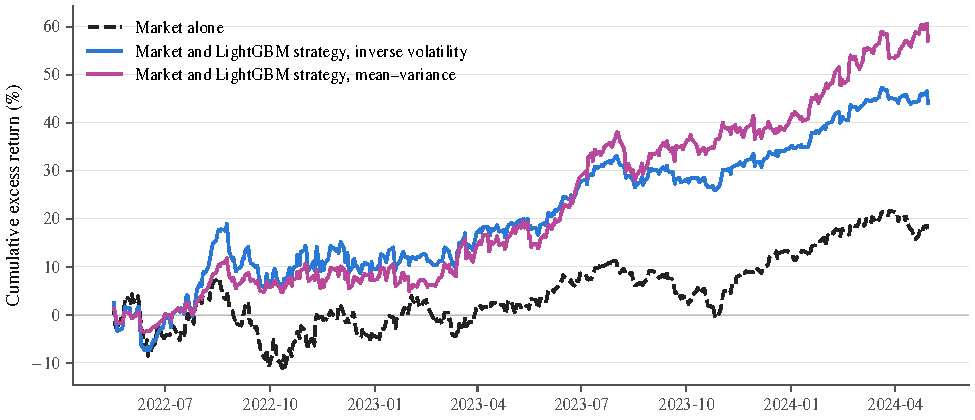
\includegraphics[width=\linewidth]{generated/rehaul_econ_beta_cum.pdf}
\caption{Cumulative excess return of the market alone and of its real-time combinations with the sign strategy of the pooled intraday LightGBM forecast on the full predictor set, at mid-quotes, on the \rhebNRt{} days from \rhebRtFirst{} (Table~\ref{tab:rh_econ_beta}, Panel C). Each series is the sum of its daily excess returns, scaled to the standard deviation of the market's daily excess return over these days, so the lines differ by their Sharpe ratios: \rhebSRmRt{} for the market, \rhebRtIvLgbmFull{} with inverse-volatility weights and \rhebRtMvLgbmFull{} with mean--variance weights (annualized by $\sqrt{q}$, $q = \rhebQRt$).}
\label{fig:rh_econ_beta_cum}
\end{figure}


% 2026-10-26 (integration, JFEc): moved here from 07_economics.tex (Results, Relation to intraday option-return
% prediction; added there 2026-10-25: a moderate comparison with Maisch, Zhang, Ulrich and Zimmer, SSRN 7269778;
% qualitative only, so no number of theirs is printed). The comparison in the conclusion stays with FRONT.
\subsection{Relation to intraday option-return prediction}
\label{app:rh_econ_maisch}
% 2026-10-26 (integration, coordinator: bullet structure): the prose recast as bold-lead items with sub-items,
% content kept.
\begin{itemize}
\item \textbf{Their design.} \citet{MaischZhangUlrichZimmer2026} also trade S\&P~500 index options on half-hourly
  machine-learning forecasts, but they forecast the delta-hedged return of each contract from its characteristics
  and sort the contracts into decile long--short portfolios every half hour. Their portfolio returns are computed at
  mid-quotes, and they note that trading each option at its quoted bid and ask prices would erase a large share of
  the profits.
\item \textbf{How ours differs.} Our test differs in three respects:
  \begin{itemize}
  \item the forecast is the variance of the underlying over the closing half hour, set against the straddle's
    implied variance;
  \item the position is a single at-the-money 0DTE straddle a day, entered at 15:30 and held to expiration;
  \item its Sharpe ratios are reported at quoted bid/ask prices as well as at mid-quotes.
  \end{itemize}
\item \textbf{Comparability.} Because the two designs differ in horizon, position, and sample period, their Sharpe
  ratios are not directly comparable.
\end{itemize}
